\documentclass{article}



% Language setting
\usepackage[english]{babel}
\usepackage[T1]{fontenc}
\usepackage[utf8]{inputenc}
\setlength{\parindent}{0pt}

% Useful packages
\usepackage{amsmath}
\usepackage{graphicx}
\usepackage{float} % Allows strict image placement
\usepackage[colorlinks=true, allcolors=blue]{hyperref}% hyperref makes the TOC clickable
\usepackage[most]{tcolorbox}
\usepackage{xcolor}
% Fonts
\usepackage[scaled]{helvet}

\usepackage{pdflscape}  % or \usepackage{lscape}
\usepackage{lipsum} % for dummy text
\usepackage{longtable}
\usepackage{caption}
\usepackage{multirow}
\usepackage{tocloft}     % Customize LoT and LoF formatting

% Better paragraph columns + hyphenation
\usepackage{ragged2e}   % gives \RaggedRight and \Centering
\usepackage{array}
\usepackage{booktabs}
\usepackage{longtable}
\usepackage{xurl}       % allows breaks in long strings (URLs-ish tokens)

% Column types (wrap-friendly)
\newcolumntype{L}[1]{>{\RaggedRight\arraybackslash}p{#1}}
\newcolumntype{C}[1]{>{\Centering\arraybackslash}p{#1}}

% Optional: allow breaks at underscores in normal text
% (useful if you *don't* typeset variable names in \texttt{})
\usepackage[strings]{underscore}


% --- Fix Roman numeral width in ToC ---
\settowidth{\cftsecnumwidth}{\bfseries XXVIII.\hspace{0.1em}}

% Geometry
\usepackage[
  a4paper,
  top=1.5in,
  bottom=1in,
  left=1in,
  right=1in,
  headheight=60pt,  % This must match the vertical space used
  headsep=20pt
]{geometry}

% Define header and footer styles
% Fancy Header
\usepackage{fancyhdr}
\usepackage{rotating}
\pagestyle{fancy}
\fancyhf{}  % clear all header/footer fields
\renewcommand{\headrulewidth}{0pt}  % no horizontal line
% Header setup
\fancyhead[C]{%
  \makebox[\textwidth]{%
    
\includegraphics[height=35pt]{resources/rufas.png}\hfill
    \textbf{\today}%
  }\\
  \textbf{Scientific Documentation of RuFaS Model}\\
  \rule{\textwidth}{1pt}
}


% Footer setup with a divider line and two lines of text on left and right
\renewcommand{\footrulewidth}{0.4pt}
\fancyfoot[L]{%
  \begin{tabular}[t]{@{}l@{}}
    Ruminant Farm System\\
    Sci Doc v.1
  \end{tabular}%
}
\fancyfoot[C]{\thepage} % Center: page number
\fancyfoot[R]{%
  \begin{tabular}[t]{@{}r@{}}
    \nouppercase{\leftmark}\\ % This pulls in the current section title
  \end{tabular}%
}
% Landscape pages should be blank (no headers/footers)
\fancypagestyle{landscapeplain}{
  \fancyhf{} % clear all
  \renewcommand{\headrulewidth}{0pt}
  \renewcommand{\footrulewidth}{0pt}
}


% Bibliography setup
\usepackage[
  backend=biber,
  style=authoryear,  % You can change this to numeric, apa, etc.
  natbib=true         % Enables \citep, \citet if desired
]{biblatex}

\addbibresource{resources/animal.bib}  % Your .bib file name
\usepackage{titlesec}
\usepackage{etoolbox}

% Reset subsection counter at each new section
\pretocmd{\section}{\setcounter{subsection}{0}}{}{}
\pretocmd{\subsection}{\setcounter{subsubsection}{0}}{}{}

\renewcommand{\thesection}{\arabic{section}}
\renewcommand{\thesubsection}{\thesection.\alph{subsection}}
\renewcommand{\thesubsubsection}{\thesubsection.\roman{subsubsection}}

% --- Title Formats (in size order) ---
\titleformat{\section}[block]
  {\Large\bfseries}
  {\thesection}
  {1em}
  {\raggedright} % <- key: prevents justification/stretching

\titleformat{\subsection}[block]
  {\normalsize\bfseries}   % Subsection: medium
  {\thesubsection}
  {1em}
  {\raggedright} % <- key: prevents justification/stretching

\titleformat{\subsubsection}[block]
  {\normalsize\bfseries}  % Subsubsection: smallest
  {\thesubsubsection}
  {1em}
  {\raggedright} % <- key: prevents justification/stretching

% --- Spacing for each level ---
\titlespacing{\section}{0pt}{10pt plus 2pt minus 1pt}{5pt}
\titlespacing{\subsection}{0pt}{8pt plus 1pt minus 1pt}{4pt}
\titlespacing{\subsubsection}{0pt}{6pt plus 1pt minus 1pt}{3pt}

% Optional: Keep your TOC control if needed
\usepackage[lof,lot]{etoc}
\etocsetlocaltop{part}
% Optional: If using headers/footers
\renewcommand{\sectionmark}[1]{\markboth{#1}{}}


% Remove default date from title
\date{} % Prevents date from appearing in \maketitle


% Define title
\title{\textbf{}}
\author{ }
\setlength{\topskip}{10pt}  % Ensures LaTeX reserves room above the first line
%\usepackage{showframe}



\begin{document}

% Custom Title Page
\begin{titlepage}
  \thispagestyle{empty}
  \centering
  \vspace*{2cm}

  {\Huge\bfseries Ruminant Farm System Model\par}
   {\Huge\bfseries (RuFaS)\par}
  \vspace{0.5cm}

 {\Large Scientific Documentation\par}
  \vspace{1cm}



  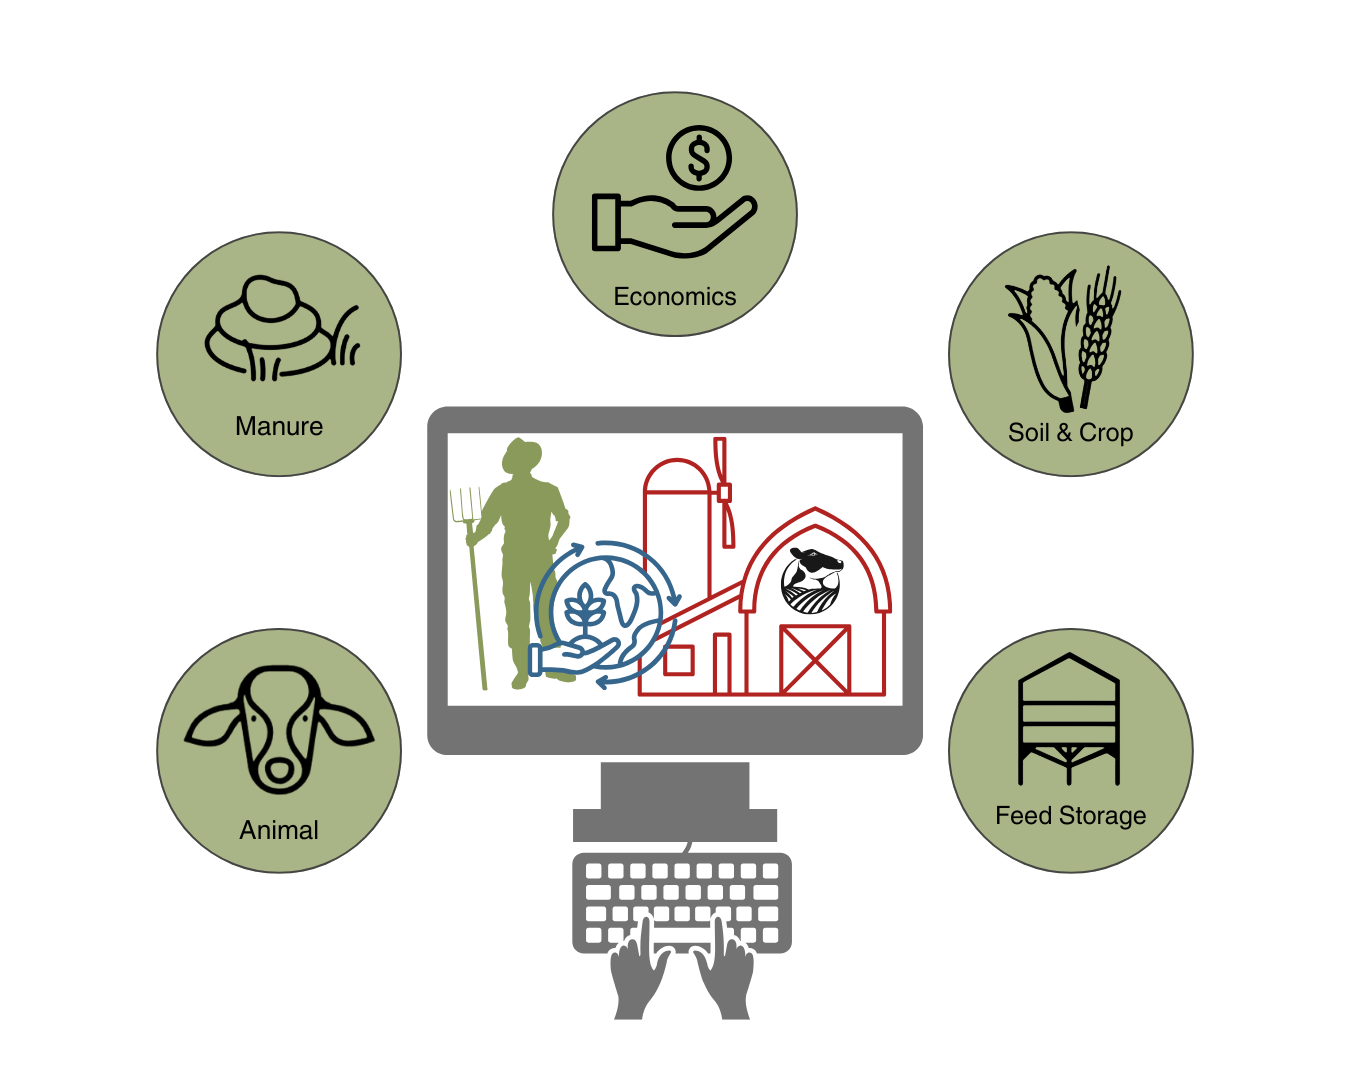
\includegraphics[width=1\textwidth]{resources/rufastitlepgimg.png} % Adjust size and filename
  \vspace{1cm}
  \vfill

  {\small v.1; Updated \today\par}
  \vspace*{1cm}
\end{titlepage}
\newpage


\setcounter{tocdepth}{2} % includes \part (-1) and \section (1), excludes \subsection (2+)
\tableofcontents
\clearpage

% --- Preface  ---
\part{Preface: A Day in the Life on a RuFaS Farm}\label{rufasday}

This document provides a high-level overview of the daily operations of a ruminant farm, as modeled by RuFaS. The overview will be through the eyes of Dr. Rue Fas. One day, Dr. Rue woke up and decided the life of a computer scientist wasn’t for her. So she bought a dairy farm, and this is how she operates it every day.

\paragraph{Feeding the Animals}
Second thing in the morning, after coffee, Dr. Rue checks the calendar to see if it’s time to formulate a new ration for her animals.
\vspace{0.2cm}

If a new ration needs to be formulated, Dr. Rue heads over to the barn where she keeps all her forages and feed. While there, she checks how well all the forages are holding up. After considering the feeds available, the quality of each one, and how much each one costs, she decides on how productive she wants her animals to be. It is a difficult balancing act, but eventually a ration recipe is found that will keep the animals happy while keeping costs low and sustainability high until the calendar says the ration recipe needs to be reformulated.
\vspace{0.2cm}

When Dr. Rue doesn’t need to formulate a new ration, she takes the last ration recipe she made and grabs all the feed and forage the animals need for the day out of the feed barn. If there isn’t enough for the animals, then a new ration is formulated using the steps above.

\paragraph{Taking Care of the Animals}
After making sure all the animals’ feed is taken care of, Dr. Rue moves on to taking care of all the other animal tasks. This includes milking the animals, making sure they’re healthy, getting them pregnant, and numerous other tasks. 
\vspace{0.2cm}

As dawn breaks on the RuFaS farm, the animals awaken after a restful night. Joe, the farm master, prepares a large whiteboard to track HerdReproductionStatistics, ensuring he has all the data he needs for the day’s activities.

\textit{Daily Routine} - After leaving their pens, each animal lines up in front of the barn. Julie, the diligent farm veterinarian, examines them one by one. This daily check includes updates on the following areas:
\begin{itemize}
    \item Nutrients: Each animal begins its day with a quick phosphorus requirement assessment. Julie records these details and updates the animal’s phosphorus-related metrics.
    \item Digestive System: With nutrient information in hand, Julie shifts focus to each animal’s digestive system, estimating manure output and enteric methane production for that day.

    \item Milk Production: All milking cows are assessed to gauge daily milk yield and milk component content (fat and protein). Any necessary adjustments are noted.

    \item Animal Growth: Around midday, Julie returns to each animal to evaluate daily weight changes. She updates each animal’s body weight accordingly.

    \item Reproduction: HeiferII and Cow stage animals undergo a reproduction check. Julie closely monitors their reproductive progress and updates the HerdReproductionStatistics details on Joe’s whiteboard.

    \item Life Stage Evaluation: Once the daily routines are complete, Julie determines if any animal is ready to progress to the next life stage. Graduating animals are marked as “graduated” to be moved to their new pens. Animals that must leave the herd—due to health, productivity, or other issues—are labeled as “sold” or “dead” to be removed from the farm population.

    \item Herd Size Maintenance: After every animal has been evaluated, Joe counts the herd to ensure it remains at a healthy size. If it is too large, he arranges the sale of some animals. If the herd is too small, he may opt to purchase additional heiferIIIs to keep numbers at the ideal level.

    \item Herd Structure Management: Joe also manages pen assignments. Newly graduated or newborn animals are guided to suitable pens, while animals marked for removal (sold or deceased) are taken out of the herd and removed from the farm records.
\end{itemize}


\textit{Output Reporting}
At day’s end, Joe and Julie review the updated HerdReproductionStatistics on the whiteboard. Joe then compiles a concise report summarizing the day’s herd stats. He forwards this information to the OutputManager before wrapping up another successful day on the RuFaS farm.
\vspace{0.5cm}

\paragraph{Dealing with the Manure}
Once all the animal chores are finished, Dr. Rue moves on to handling the manure. There are a lot of different ways that manure is collected from the animals: it is flushed out of the milking parlor with water, some of the pens need to have it shoveled out along with the bedding in the pen, and some pens have grates that allow the manure to go straight into a pit beneath the barn.
\vspace{0.2cm}

There are a lot of different places where manure is processed and stored on the farm. Dr. Rue goes from place to place on the farm, moving the manure from one place to the next. The manure chores are finished after moving all of the manure into her lagoons, compost piles, and other storages. As this final manure chore is completed, she writes down all the information about how much manure is in all these storages, and some information about what that manure is made of. How much water, nitrogen, phosphorus, other solids, etc. are in each storage.

\paragraph{Managing the Fields}
Now that Dr. Rue is done making sure all the manure has been handled and stored properly, she can take care of all the field tasks. She has a lot of fields on her farm, each with its own unique schedule. Her field management routine starts with checking each field’s schedule to see if any of them are due to have manure applied, and if so, how much they should have applied. After noting all the manure that is supposed to go onto her fields, these amounts are checked against the amounts of manure that are in her manure storage. Dr. Rue then applies manure to each field on the schedule that day, trying to match the amount applied to the amount on the schedule as best she can.
\vspace{0.2cm}

After making sure every manure item on each farm’s schedule has been taken care of for the day, the schedule for each field is rechecked, one field at a time. In each schedule she checks to see if that field needs to be tilled, if any chemical fertilizer needs to be applied, and if any crops need to be planted or harvested. After all these activities are taken care of, Mother Nature goes to work. The sun shines and rain falls, providing the field with water and energy that grows crops and soaks the soil. After taking care of each field one by one, Dr. Rue drives back to the main farm with all of the crops that she harvested on that day.

\paragraph{Storing the Feeds}
Now that she is back at the barns, all the crops that were just harvested can be stored. Fortunately she is very organized, so all her harvested crops are separate from one another and each has a label, indicating where it will be stored inside the feed barn. As each feed is stored, it is labeled with the current date. Dr. Rue is exhausted from another long day. She goes back to the farmhouse and rests up, preparing to do the whole thing over again tomorrow. Her daily routine might seem repetitive, but each day is a crucial part of the larger, continuous process that keeps her farm running efficiently and sustainably.



\newpage
\part{Animal Module}
% Global Table of Contents
\thispagestyle{fancy}

% Local TOC that includes only what’s inside THIS section
\etocsettocstyle{\subsection*{Contents}}{} % heading for the local toc
\etocsetnexttocdepth{subsection}           % or subsubsection
\localtableofcontents
\newpage

\section*{List of Figures}
\locallistoffigures
\newpage

\section*{List of Tables}
\locallistoftables
\newpage


\section{Module Introduction}
\begin{refsection}
    \par\noindent\justifying
  The Animal Module simulates individual animals on a daily basis throughout each stage of life from birth until removal from the herd. In addition to the dynamic Monte-Carlo models that determine the occurrence of events throughout each animal’s life, the Animal Module uses process-based, dynamic models to simulate the following processes:

\begin{figure}[H]
\centering
\begin{minipage}[t]{0.35\textwidth}
  \vspace{0pt} %ensures no vert offset
  \centering
  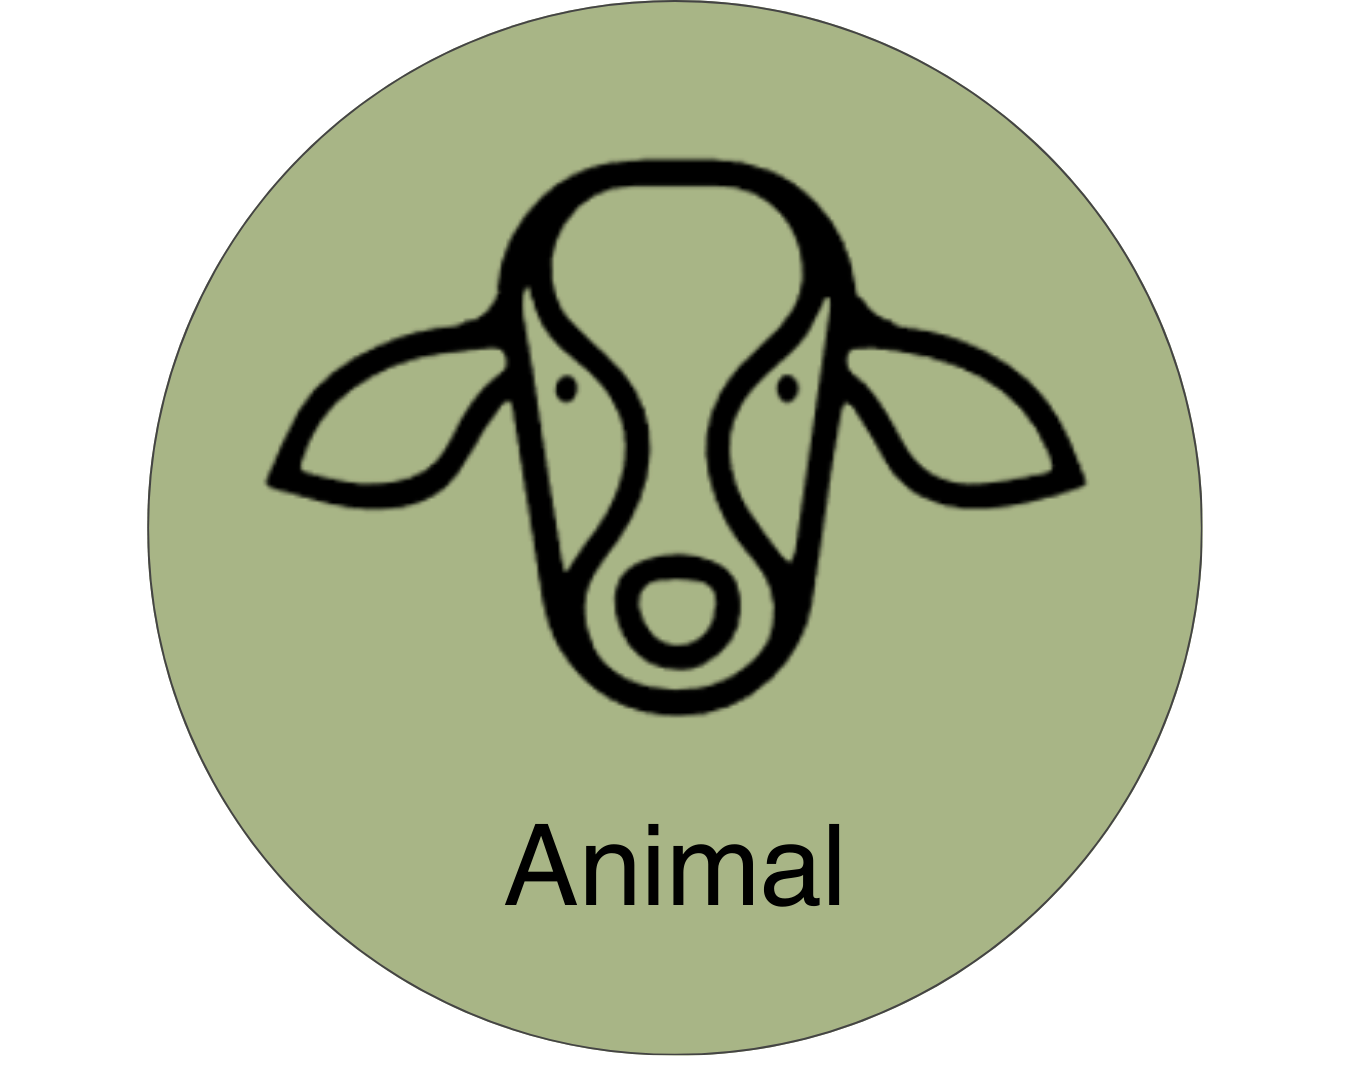
\includegraphics[width=0.4\linewidth]{resources/animal1.png}
\end{minipage}%
\hfill
\begin{minipage}[t]{0.6\textwidth}
  \vspace{0pt}

  \begin{itemize}
      \item Individual animal growth
      \item Gestation and milk production
      \item Estimation of nutrient requirements and feed intake
      \item Enteric emission and manure excretion 
  \end{itemize}
\end{minipage}
\end{figure}
\par\noindent\justifying

Animals in the RuFaS model are divided into 5 life stages and a culling stage that were established based on the different management and physiological processes that need to be simulated for each class. The 5 classes and culling stage are described in more detail later in this document, but include: calves, heifers I, heifers II, heifers III, cow, and culled. 

The attributes that define the animal characteristics and management are provided by the user and are comprehensively described in the inputs section of this module. When a simulation begins, the herd is populated by a semi-random draw of animals from a large, existing set of animal objects. This process and the process for regenerating the population of animals used to initialize the herd are described in detail in the \hyperref{herdinit}{Herd Initialization Section}. The initially selected animal objects are then grouped into pens based on their life stage and the user-provided pen information. Once the herd has been set up, a regular progression of functions is called each day to simulate and report outputs of the processes required to manage the herd and the processes that define each animal’s development and production. These daily updates are grouped into two classes in the RuFaS model: herd level daily routines (HerdManager) and animal level daily routines (AnimalManager). At the start of each day, the Herd-level daily update cycles through all the animals to call their daily update functions. Then based on the changes for each animal that resulted from the animal level daily updates, the HerdManager changes the animal life-stages, moves them to new pens, and removes them from the herd. If the herd size has decreased too much, the HerdManager will purchase new Heifer III animals to maintain the adult herd size. The HerdManager then checks if it is time to formulate a new diet (at a user-specified interval), summarizes and reports the herd statistics, and gathers and reports all of the manure excreted by the animals to pass to the Manure Module. 

Daily outputs from the Animal module are provided at a variety of scales and time steps that range from reports at the individual animal level (e.g. animal event histories), animal class level (e.g. average dry-matter intake for Heifer II’s), at the pen level (e.g. average net energy requirement or intake for Pen 3), and at the herd level (i.e. number of animals sold each day). A complete list of potential outputs from the Animal Module is provided in this document.
\vspace{1cm}


\subsection{Animal Life Cycle}
\vspace{0.2cm}

The animal life cycle is driven by Monte Carlo stochastic processes that simulate the growth, production, reproduction, and culling of individual dairy cattle animals and shares aggregated outcomes with the herd management sub-module to manage herd dynamics on a daily basis. 
 
The life cycle module represents the variation in animal performance through the use of Monte Carlo Simulation methods \parencite{reuven2017}. Monte Carlo simulation relies on random draws from probability distributions rather than assigning fixed values. In this model, two main strategies are used:
\begin{itemize}
    \item Event-based, in which a random draw from a uniform distribution (U(0,1)) is compared to the probability of an event occurring to simulate if that event occurs, and 
    \item Population-based, in which a random draw from a known distribution of attribute values is assigned to an animal at instantiation. Probability distributions used for that purpose are Normal Gaussian or Empirical. 
\end{itemize}

Each animal within the RuFaS herd progresses through five main life stages (calf, Heifer I, Heifer II, Heifer III, and Cow) as illustrated in the figure below. 
\begin{itemize}
    \item Calves progress to Heifer I when their age reaches the user-defined input for weaning day
    \item Heifer I progresses to Heifer II when their age reaches the user-defined input for breeding start day 
    \item Heifer II animals that successfully conceive become Heifer III's when the number of days left in their pregnancy is equal to the user-defined input for prefresh days (default 21)
    \item When a Heifer III calves, she becomes a Cow for the rest of her life on the RuFaS farm
    \item Cows cycle through lactating and non-lactating phases until they are removed from the herd due to a failure to conceive or a user-provided probability for sale or death within each parity (lactation).

\end{itemize}

When a HeiferIII or Cow reaches full gestation length, they start lactating and a new calf object is created. The calf is assigned a birthweight according to a user-informed random distribution. All male calves are recorded and removed from the farm on day 1 of their life. Female calves either remain on the farm or are sold on day 1, determined by an event-based Monte Carlo method informed by the user-defined percent of female calves that are kept. 



\section{Herd-level Processes and Management}
\vspace{0.5cm}

\subsection{Herd Initialization} \label{herdinit}
\vspace{0.5cm}

\begin{tcolorbox}[colback=white, colframe=black, title=Important Note]
\textit{In RuFaS code, the term “herd initialization” is used to refer to both the process of generating an animal population file and of selecting from that population to create a specific herd at the start of a simulation. In this doc, those two processes will be differentiated by calling them “Generation” and “Selection”, respectively. }
\vspace{0.2cm}

\textit{“Animal population” can refer to both groups of animals (the pool of animals generated, and the herd of animals selected). In the code, the population is sometimes referred to as “pre\_animal\_population” and “post\_animal\_population” to differentiate whether the specified group of animals exists before or after the random selection of individuals to create a herd. }
\end{tcolorbox}
\vspace{0.2cm}

\paragraph{Introduction}

Every simulation begins with a herd consisting of calves, heifers, and dry and lactating cows. This herd comes to be through a two-step process: 
\begin{enumerate}
    \item A population of animals is generated through simulation or loaded from data (pre-animal-population). The animals in that herd should reflect the attributes of animals in the herd to be modeled. 
    \item Animals are randomly selected with replacement from the pre-animal-population to be in the initial herd, based on group numbers and characteristics that reflect the distribution of animals within the herd being modeled. Note that the animals in the herd on day one will have attributes of the pre-animal-population and may deviate from the desired herd to be modeled.  
\end{enumerate}

For the rest of the simulation, animals enter the herd through birth as newborn calves or purchased replacements (heiferIII’s). 


% assumes \newcolumntype{L}[1]{>{\raggedright\arraybackslash}p{#1}}
\renewcommand{\arraystretch}{1.4}

\begin{longtable}{@{} L{5cm} L{5cm} L{5cm} @{}}
\caption{Overview of the distinct phases by which animals are created and introduced to the herd.}\\
\toprule
\multicolumn{1}{c}{\textbf{Before the simulation}} &
\multicolumn{1}{c}{\textbf{At the initiation of simulation}} &
\multicolumn{1}{c}{\textbf{During the simulation}}\\
\midrule
\endfirsthead

\multicolumn{3}{@{}l}{\textit{Table continued from previous page}}\\
\toprule
\multicolumn{1}{c}{\textbf{Before the simulation}} &
\multicolumn{1}{c}{\textbf{At the initiation of simulation}} &
\multicolumn{1}{c}{\textbf{During the simulation}}\\
\midrule
\endhead

\midrule
\multicolumn{3}{r@{}}{\textit{Continued on next page}}\\
\endfoot

\bottomrule
\endlastfoot

Generate (simulate) or load an Animal Population file (pre-animal-population).  
\vspace{0.1cm}

The animals present at the start of the simulation, and those available in the replacement market, are drawn from this file. &%

Herd is established by random selection of animals from the Animal Population to match the user-specified group sizes and age/stage distribution (post-animal-population).  
\vspace{0.1cm}

Management attributes—including lactation-curve parameters—are assigned as each animal enters the herd. &%

New animals enter via \textbf{(a)} birth or \textbf{(b)} purchase of heifers from the replacement market.  
Purchased animals inherit two attributes from the population file:
\begin{minipage}[t]{\linewidth}
\begin{itemize}
  \item Breed
  \item Mature body weight
\end{itemize}
\end{minipage}\\

\end{longtable}



\newpage
\begin{landscape}
% Suppress header/footer for all pages of the longtable
\fancypagestyle{landscapeplain}{
  \fancyhf{} % clear header and footer
  \renewcommand{\headrulewidth}{0pt}
  \renewcommand{\footrulewidth}{0pt}
}

\pagestyle{landscapeplain} % Apply to all pages in this landscape block
\textbf{Required User Inputs}
% assumes \newcolumntype{L}[1]{>{\raggedright\arraybackslash}p{#1}}
\renewcommand{\arraystretch}{1.4}

\begin{longtable}{@{} L{5cm} L{7cm} C{2cm} C{2cm} C{2cm} @{} }
\caption{User inputs in the animal input file that influence the generation of the Animal Population (pre-animal-population). The inputs of this table are found in the Herd Initialization Section}\\
\toprule
\multicolumn{1}{c}{\textbf{Variable}} &
\multicolumn{1}{c}{\textbf{Definition}} &
\multicolumn{1}{c}{\textbf{Default}} &
\multicolumn{1}{c}{\textbf{Min}} &
\multicolumn{1}{c}{\textbf{Max}}\\
\midrule
\endfirsthead

\multicolumn{3}{@{}l}{\textit{Table continued from previous page}}\\
\toprule
\multicolumn{1}{c}{\textbf{Variable}} &
\multicolumn{1}{c}{\textbf{Definition}} &
\multicolumn{1}{c}{\textbf{Default}} &
\multicolumn{1}{c}{\textbf{Min}} &
\multicolumn{1}{c}{\textbf{Max}}\\
\midrule
\endhead

\midrule
\multicolumn{3}{r@{}}{\textit{Continued on next page}}\\
\endfoot

\bottomrule
\endlastfoot

Initial\_animal\_num & The initial number of animals that serve as a starting point for the population generation simulation & 10000 & 0 & -  \\
Simulation\_days & The number of days to simulate for the population generation simulation & 5000 & 0 & -   \\

\end{longtable}
\vspace{-0.75cm}

\renewcommand{\arraystretch}{1.4}

\begin{longtable}{@{} L{5cm} L{7cm} C{2cm} C{2cm} C{2cm} @{} }
\caption{User inputs in the animal input file that influence the generation of the Animal Population (pre-animal-population). The inputs of this table are found in the Herd Initialization Section.}\\
\toprule
\multicolumn{1}{c}{\textbf{Variable}} &
\multicolumn{1}{c}{\textbf{Definition}} &
\multicolumn{1}{c}{\textbf{Default}} &
\multicolumn{1}{c}{\textbf{Min}} &
\multicolumn{1}{c}{\textbf{Max}}\\
\midrule
\endfirsthead

\multicolumn{5}{@{}l}{\textit{Table continued from previous page}}\\
\toprule
\textbf{Variable} & \textbf{Definition} & \textbf{Default} & \textbf{Min} & \textbf{Max} \\
\midrule
\endhead

\midrule
\multicolumn{5}{r@{}}{\textit{Continued on next page}}\\
\endfoot

\bottomrule
\endlastfoot

Calf\_num & Number of Calves (head) -- The initial number of pre-weaned calves & 8 & 2 & -- \\
HeiferI\_num & Number of HeiferI animals (head) -- The initial number of heifers that are weaned but not yet bred & 44 & 2 & -- \\
HeiferII\_num & Number of HeiferII animals (head) -- The initial number of heifers that are either eligible for breeding (based on user-inputted Breeding Start Day for heifers), or in early pregnancy & 38 & 2 & -- \\
HeiferIII\_num\_springers & Number of HeiferIII animals (head) -- The initial number of close-up heifers (within the user-defined close-up period, e.g., Prefresh Day) & 5 & 2 & -- \\
Cow\_num & Number of Cows (head) -- The initial number of dry and lactating cows & 100 & 6 & -- \\
Replace\_num & Replacements (head) -- Number of replacement animals available in the replacement market & 5000 & 50 & -- \\
Lactating\_fraction & Fraction of cows that are lactating. Used during herd initialization & 0.8356 & 0 & 1 \\
Parity\_fractions: 1, 2, 3, 4, 5 & Fractions of the milking animal population that are parity 1, 2, 3, 4, and 5+. The sum must equal 1.0 & 0.36, 0.26, 0.18, 0.11, 0.09 & 0 & 1 \\

\end{longtable}



\end{landscape}


\textbf{Relevant Outputs}

After the animals have been selected from the animal population to create the initial herd, a summary of the Population (pre-selection pool, aka pre-animal-population) and of the Initial herd (selected animals, aka post-animal-population) is provided to the output manager. 
\vspace{0.2cm}

Class and function: AnimalModuleReporter.report\_animal\_population\_statistics
Output variables: 
\begin{itemize}
    \item .population\_{...}
    \item .initial\_{...}
\end{itemize}

{...} includes: breed, number of animals of each class (calf, heiferI, heiferII, heiferIII, cow), number of cows by parity and lactation status, average age of animals within each class, distribution of age of animals within each class, average body weight of animals within each class, average cow days in milk, days in preg, parity, and calving interval. 




\paragraph{Methodology}

When a simulation begins, the HerdFactory class generates or loads the pre-animal-population, from which it selects and compiles the post-animal-population with an appropriate distribution of animal ages and stages to serve as the starting herd for simulation. 
\vspace{0.3cm}

\textbf{\textit{Designation of an Animal Population}}
\vspace{0.3cm}

\textbf{Option 1:} Creating a new Animal Population
An animal population can be generated as a stand-alone simulation task that creates and saves a pre-animal-population file  as the output based on the user Animal Module inputs. Or, the animal population can be generated as the first step of a regular simulation task which then uses that generated pre-animal-population to select from and create the post-animal-population to use for the subsequent herd simulation. See the documentation about Task Manager for more information about how to generate a new pre-animal-population. 
\vspace{0.2cm}

The \_generate\_animals() method creates the pre\_animal\_population, with the option to save those animals to file at the end of the generation process. 
\vspace{0.2cm}

Calves are created according to the number specified by the user (initial\_animal\_num), some are sold based on user inputs, and those remaining proceed through select daily updates (growth, reproduction, milk, and transition through the appropriate life stages) for the user-specified number of days (simulation\_days). The simulation occurs similarly to the regular life cycle simulation process, but with an extended period and large number of animals. There are a few notable distinctions:  
\begin{itemize}
    \item After 3000 days of simulation (specified in animal\_constants), a copy of each heiferIII is saved to the replacement herd. The copy is made on the day when she is ready to transition to a lactating cow (ready to give birth), so that when the copy enters the herd as a purchased heiferIII during the actual simulation, she will give birth the very next day. 
    \item If a cow has made it to parity six without being culled, she is removed from the herd. (The maximum parity of cows kept in the generated herd is five). 

\end{itemize}

After the simulation\_days number of days, the full herd contains a mixture of calves, heifers, cows, and replacements. The core status information and life history of each animal are either saved to file or passed for random sampling to create the post-animal-population. 
\vspace{0.2cm}

\textbf{Option 2:} Point to an existing Animal Population
Alternatively, the pre-animal-population will be loaded from a specified Animal Population input file consisting of calf, heifer, cow, and replacement objects. 
\vspace{0.2cm}

\textit{Herd Selection}
The \_random\_sample\_with\_replacement() method selects animals from each of the following groups: calf, heiferI, heiferII, heiferIII, replacement, lactating cows by parity for parities 1-5, and dry cows by parity for parities 1-5. Animals are sampled randomly with replacement from the pre-animal-population according to the numbers, parity fractions, and milking cow fraction specified in the animal input file. The resulting list of animals is returned as the post-animal-population and summaries of the pre- and post-animal-populations are reported to the output manager.



\subsection{Pens and Animal Grouping}

 
    \paragraph{Introduction} All animals in RuFaS are assigned to a pen which is used to summarize nutrient requirements for diet formulation and feeding, aggregate enteric methane and manure excretions for reporting and passage to the Manure Module. Each pen tracks and updates daily a list of animals in the pen, the stocking density, the average nutrient requirement of the animals in the pen, the ration being fed to that pen, the manure excreted, and the methane emitted. In addition, constant attributes of each pen include the type of pen it is (freestall, tiestall, open lot, compost bedded pack barn), the type of animals that can be in that pen, the number stalls, the manure management practices associated with that pen, and the distance to the milking parlor for lactating cows.  Each day after the HerdManager has updated the status of each animal and determined which animals need to be bought or sold, the animals are added and removed from pens as needed. 

\newpage
\begin{landscape}
% Suppress header/footer for all pages of the longtable
\fancypagestyle{landscapeplain}{
  \fancyhf{} % clear header and footer
  \renewcommand{\headrulewidth}{0pt}
  \renewcommand{\footrulewidth}{0pt}
}

\pagestyle{landscapeplain} % Apply to all pages in this landscape block

% Begin longtable
\textbf{Required User Inputs} 
\begin{center}
    \captionof{table}{The user must define at least 3 pens and for each pen, key inputs are:} 
\end{center}
\renewcommand{\arraystretch}{1.4} % More vertical space between rows
\begin{longtable}{@{} L{5cm} L{7cm} C{2cm} C{2cm} C{2cm} @{} }

\toprule
\multicolumn{1}{c}{\textbf{Variable}} & 
\multicolumn{1}{c}{\textbf{Definition}} &
\multicolumn{1}{c}{\textbf{Default}} &
\multicolumn{1}{c}{\textbf{Min}} &
\multicolumn{1}{c}{\textbf{Max}} \\
\midrule
\endfirsthead

\multicolumn{5}{@{}l}{\textit{Table continued from previous page}} \\
\toprule
\multicolumn{1}{c}{\textbf{Variable}} & 
\multicolumn{1}{c}{\textbf{Definition}} &
\multicolumn{1}{c}{\textbf{Default}} &
\multicolumn{1}{c}{\textbf{Min}} &
\multicolumn{1}{c}{\textbf{Max}} \\
\midrule
\endhead

\midrule
\multicolumn{5}{@{}r@{}}{\textit{Continued on next page}} \\
\endfoot

\bottomrule
\endlastfoot


id  & The index of the pen  & NA  & 0 & NA \\

pen\_name  & The name or identifier of a given pen  & NA  &  &  \\

animal\_combination  & The valid combinations of animal types that can be in a pen. CALF = Calves; GROWING = HeiferI's and HeiferII's; CLOSE\_UP = HeiferIII's and Dry Cows; LAC\_COWS = Lactating Cows  &    &  \multicolumn{2}{C{6cm}}{CALF, GROWING CLOSE\_UP, LAC\_COW} \\

vertical\_dist\_to\_milking\_parlor  & The elevation gain (in meters) between the pen and the milking parlor  & 0.1  &  0 & NA \\

horizontal\_dist\_to\_milking\_parlor  & The distance (in meters) between the pen and the milking parlor & 10  &  0 & NA \\

number\_of\_stalls  &  The number of stalls in the pen & 1000  &  0 & NA \\

pen\_type  &  The type of pen (freestall, tiestall, open lot, compost bedded pack barn) & freestall  & \multicolumn{2}{C{6cm}}{freestall, tiestall, open lot, compost bedded pack barn} \\

max\_stocking\_density  &  The maximum ratio of the number of animals in the pen to the number of stalls in the pen & 1.2  &  0.5 & 5 \\

manure\_management\_scenario\_id &  The ID number of the manure management practices that are used for this pen (scenarios are defined in manure management schema) & 0  &  0 & NA \\

\end{longtable}
\end{landscape}


    \textbf{Relevant Outputs}
    \begin{itemize}
        \item \textbf{number\_of\_animals\_in\_pen\_[id]\_[AnimalCombination]} reports the number of animals in each pen each day.

        \item \textbf{ration\_per\_animals\_for\_pen\_[id]\_[AnimalCombination]} - reports average dry matter intake of an animal in the pen at the time of the ration formulation.

        \item \textbf{ration\_per\_animals\_for\_pen\_[id]\_[AnimalCombination].[RUFAS\_feed\_id]} - reports the amount of each feed that is delivered per animal in the pen

        \item \textbf{ration\_nutrient\_amount\_for\_pen\_\_[AnimalCombination].[nutrient]} - is reporting the amount of each of the following nutrients that is provided by the ration per animal in the pen (all reported in kilograms unless otherwise indicated):
    \end{itemize}
    
    
\paragraph{Methodology}

\textbf{\textit{Animal Grouping}} To translate from the AnimalTypes needed to track an animal’s life stages and the combinations of animals that are allowed to be grouped into a single pen, a new variable called AnimalCombination is created that combines some AnimalTypes to facilitate sorting into pens. The AnimalCombination class is defined in enums.py and includes the following mapping from AnimalTypes to AnimalCombinations:

\begin{table}[h!]
\centering
\renewcommand{\arraystretch}{1.3}
\caption{A summary of animal types}
\begin{tabular}{@{} L{4.5cm} L{3.5cm}  @{}}
\toprule

\multicolumn{1}{c}{\textbf{Animal Combination}} &
\multicolumn{1}{c}{\textbf{Animal Types}} \\
\midrule
CALF  & Calves  \\
GROWING  & Heifer I and Heifer II  \\
CLOSE\_UP  & Heifer III and Cows (non-lactating)  \\
LAC\_COW  & Cows (lactating)  \\
\bottomrule
\end{tabular}
\end{table}  

 
 Currently there are only two options for assigning AnimalCombinations to pens. 
\vspace{0.2cm}
\begin{itemize}
    \item \textit{Option 1} - The first and most commonly used option for grouping animals is to assign one AnimalCombination to each pen such that there is at least one pen for the 4 AnimalCombinations: CALF, GROWING, CLOSE\_UP, and LAC\_COW. 
    \item \textit{Option 2} - In some cases, and especially in very small farms, a user might wish to represent a scenario where all growing animals, pregnant heifers, and non-lactating cows are housed together. In this case, there is an option to have a pen that houses both GROWING and CLOSE\_UP animals such that the there is at least one pen with each of the 3 AnimalCombination inputs: CALF, GROWING\_AND\_CLOSE\_UP, and LAC\_COW. 
\end{itemize}


    \textbf{\textit{Pen Sizing}} Due to oscillations in the exact number of animals in each animal type, it is strongly recommended that the stocking density is at least 120\% of the expected number of animals in each pen. 
    \vspace{0.2cm}
    
    \textbf{\textit{Class}} 
    \vspace{0.2cm}
    
    \textbf{Pen}
    Pens are initiated from the Pen class by the HerdManager at the beginning of the simulation and, if needed, an additional pen is created to accommodate animals if the animal numbers have exceeded the max stocking density. 

    \textbf{\textit{Noteworthy Functions}} 
    \vspace{0.2cm}
    
    \paragraph{Remove\_animals\_by\_ids} This function is called when the HerdManager calls for: remove\_animal\_from\_pen\_and\_id\_map. It is pen specific and removes the animal from the pen and the animal ID from the animal ID map that tracks the animals in the pen. 


    \paragraph{\_add\_new\_animals}This function is called by Pen.update\_animals which is in turn called by HerdManager.\_add\_animal\_to\_pen\_and\_id\_map. Thus, when HerdManager initiates addition of animals to each pen, this function executes the addition of those animals. 

    \paragraph{Set\_animal\_nutritional\_requirements}


\subsection{Ration Formulation}
The diet recipes in RuFaS are either formulated through least-cost formulation \parencite{Li2022} or provided by the user for each of 4 animal categories (calves, growing heifers, dry and close-up cows, and lactating cows). The composition of the available feeds are provided by a feed library that was adapted from the \cite{nrc2021}. The amount of feed required by the farm is tracked by pen and multiple pens of each animal category can be simulated; however, at this time, the RuFaS model can only accept 1 user-defined diet per animal category even if there are multiple simulated pens for that animal category.  

In practice, animal feeding on dairy farms is a constantly evolving process that responds to fluctuations in feed availability, animal requirements and responses, and management goals. Although the feed delivery algorithms will make small modifications to the diet recipe in response to animal nutrient requirements and adjust the total amount of feed delivered based on the number of animals and their requirements, the diversity and degree of fluctuation in the diets is less than what is expected on a commercial dairy. The RuFaS feed library can also be modified or expanded on by changing the compositions of the existing feeds or by adding new feeds. 

Regardless of whether or not a user chooses to provide their own ration or have RuFaS build and feed a ration optimized for least-cost, RuFaS needs a set of ingredients to work from. The RuFaS feed library should be consulted for the full list of ingredients and ingredients that are in both the NASEM and NRC libraries can be used. Users interested in feeding a ration that they define, need to provide a list of ingredients and their relative \% dry matter intake for each animal class (pre-weaned calves, growing heifers, close-up animals, and lactating cows). 

\vspace{0.2cm}

If a user would like RuFaS to use the list of ingredients to formulate a least-cost ration, it is imperative that proper costs are inputted for each ingredient listed, but the \% dry matter intake in the user defined ration percentages does not need to be included. Feed costs need to be entered in \$ / kg DM. RuFaS will then use all the ingredients available (based on costs and inventory available if the feed is homegrown) to create a ration that meets the nutritional requirements of the animal class and is cost-optimized. 


\begin{tcolorbox}[colback=white, colframe=black, title=Important Note]
For the time being, only one set of feeds and ration formula can be provided for each animal class. 
\end{tcolorbox}







\subsubsection{Energy and Nutrition Requirements}

\paragraph{NRC: Calculating Nutrient Requirements of Dairy Cattle} 

Below are the calculations utilized based on the energy and nutrient requirements of dairy cattle as reported by the NRC and more recently the NASEM \parencite{nrc2001, nrc2021}.
\vspace{0.2cm}

Calculations are included for the following requirement categories:
\begin{itemize}
    \item Energy (Maintenance, Activity, Growth, Pregnancy, Lactation)
    \item Protein (Maintenance, Growth, Pregnancy, Lactation)
    \item Minerals (Maintenance, Growth, Pregnancy, Lactation)
    \item Dry Matter Intake
    \item Amino Acids (NASEM only) 
\end{itemize}
\vspace{0.2cm}

Where appropriate, requirement calculations are differentiated by animal age and reproductive status.
\vspace{0.5cm}

\subsubsection{Nutrient Requirements of Dairy Cattle (NRC)} 

    \textbf{ Energy Requirements} For details about the variables included in each calculation, please refer to the energy requirements key.
    \vspace{0.2cm}
    
    \begin{itemize}
        \item \textbf{\textit{Maintenance}} - The maintenance requirement is calculated based on metabolic body weight (body weight\(^ {0.75}\)).
        
        \vspace{0.2cm}
        \underline {Lactating and Dry Cows}
        
        \vspace{0.25cm}
\begin{center}
    \(CBW = MW * 0.06275\)
\end{center}
\vspace{0.5cm}
            {\raggedleft \textbf{[AN.NRC.1]}\par}

\vspace{0.25cm}
\begin{center}
    \(CW = {(18 + (DOP - 190) * 0.665) * ( \frac{CBW}{45}), if DOP > 190.0}\)
\end{center}
\vspace{0.5cm}
            {\raggedleft \textbf{[AN.NRC.2]}\par}
\textit{\small Otherwise}
\vspace{0.25cm}

\begin{center}
    \(NEmaint = 0.08 * (BW - CW)^{0.75}\)
\end{center}
\vspace{0.5cm}
            {\raggedleft \textbf{[AN.NRC.3]}\par}

        \vspace{0.2cm}
        \underline {Heifers} -The maintenance requirement is calculated based on metabolic body weight (body weight\(^{0.75}\)), body condition score, and the previous month's temperature.
        \vspace{0.25cm}

    
\begin{center}
    \(CBW = MW * 0.06275\)
\end{center}
\vspace{0.5cm}
            {\raggedleft \textbf{[AN.NRC.1]}\par}

\vspace{0.25cm}
\begin{center}
    \(CW = {(18 + (DOP - 190) * 0.665) * ( \frac{CBW}{45}), if DOP > 190.0}\)
\end{center}
\vspace{0.5cm}
            {\raggedleft \textbf{[AN.NRC.2]}\par}
\textit{\small Otherwise}
\vspace{0.25cm}


\begin{center}
    \(BCS9 = (BCS5 - 1) * 2 + 1\)
\end{center}
\vspace{0.5cm}
            {\raggedleft \textbf{[AN.NRC.6]}\par}

\vspace{0.25cm}
\begin{center}
    \(NEmaint = (BW - CW)^{0.75} * (0.086 * (0.8 + (BCS9 - 5) * 0.05) + 0.0007 * (20 - PrevTemp))\)
\end{center}
\vspace{0.5cm}
            {\raggedleft \textbf{[AN.NRC.7]}\par}

\vspace{0.25cm}

        \item \textbf{\textit {Activity}} - Activity requirement is proportional to body weight and daily walking distance. A grazing system and hilly topography will cost additional energy. 

        \vspace{0.2cm}
        \underline {Lactating and Dry Cows}
        \vspace{0.25cm}

    
\begin{center}
    \(NEa1 = 0.0012 * BW\) if Housing = Grazing 0
\end{center}
\vspace{0.5cm}
            {\raggedleft \textbf{[AN.NRC.8]}\par}
\textit{\small Otherwise}
\vspace{0.25cm}

\begin{center}
    \(NEa2 = 0.006 * BW\) if Topography = Hilly 0
\end{center}
\vspace{0.5cm}
            {\raggedleft \textbf{[AN.NRC.9]}\par}
\textit{\small Otherwise}
\vspace{0.25cm}

\begin{center}
    \(NEa2 = 0.Distance * 0.00045 * BW + NEa1 + NEa2\) 
\end{center}

\vspace{0.5cm}
            {\raggedleft \textbf{[AN.NRC.10]}\par}
            
        \vspace{0.2cm}
        \underline {Heifers}
        \vspace{0.25cm}
        
\begin{center}
    \(NEa1 = 0.0009 * BW + 0.0016 * BW\) if Housing = Grazing 0
\end{center}
\vspace{0.5cm}

            {\raggedleft \textbf{[AN.NRC.11]}\par}
\textit{\small Otherwise}
\vspace{0.25cm}

\begin{center}
    \(NEa2 = 0.006 * BW\) if Topography = Hilly 0
\end{center}
\vspace{0.5cm}

            {\raggedleft \textbf{[AN.NRC.12]}\par}
            \vspace{0.25cm}
            
\textit{\small Otherwise}
\vspace{0.25cm}

\begin{center}
    \(NEa2 = 0.Distance * 0.00045 * BW + NEa1 + NEa2\) 
\end{center}
\vspace{0.5cm}

            {\raggedleft \textbf{[AN.NRC.10]}\par}

\vspace{0.5cm}


        \item \textbf{\textit{Growth}}
        
        \vspace{0.2cm}
        \underline {Lactating and Dry Cows} Cows will continue to grow toward their mature body weight until the end of their second lactation. 
        \vspace{0.25cm}
        
\begin{center}
    \(MSBW = 0.96 * MW\)
\end{center}
\vspace{0.5cm}
            {\raggedleft \textbf{[AN.NRC.13]}\par}

\vspace{0.25cm}
\begin{center}
    \(SBW = 0.96 * BW\)
\end{center}

\vspace{0.5cm}
            {\raggedleft \textbf{[AN.NRC.14]}\par}
\vspace{0.25cm}

\begin{center}
    \(EBW = 0.96 * SBW\)
\end{center}
\vspace{0.5cm}

            {\raggedleft \textbf{[AN.NRC.15]}\par}
\vspace{0.25cm}

\begin{center}
    \(EQSBW = (SBW - CW) *\frac{478}{MSBW} SBW\)
\end{center}
\vspace{0.5cm}

            {\raggedleft \textbf{[AN.NRC.16]}\par}
\vspace{0.25cm}

\begin{center}
    \(ADG = \frac{(0.92 - 0.82) * MSBW}{CI}, if Parity = 1 \frac{(1 - 0.92) * MSBW}{CI}, if Parity = 2.0, if Parity > 2\)
\end{center}
\vspace{0.5cm}

            {\raggedleft \textbf{[AN.NRC.17]}\par}
\vspace{0.25cm}

\begin{center}
    \(EQEBG = 0.956 * ADG\)
\end{center}
\vspace{0.5cm}

            {\raggedleft \textbf{[AN.NRC.18]}\par}
    \vspace{0.25cm}
    
\begin{center}
    \(EQEBW = 0.891 * EQSBW\)
\end{center}

\vspace{0.5cm}
            {\raggedleft \textbf{[AN.NRC.19]}\par}
\vspace{0.25cm}

\begin{center}
    \(NEg = 0.0635 * EQEBW^{0.75} * EQEBG^{1.097}\)
\end{center}

\vspace{0.5cm}
            {\raggedleft \textbf{[AN.NRC.20]}\par}
            
        \vspace{0.2cm}
        \underline {Heifers}
\vspace{0.25cm}

\begin{center}
    \(ADG = \frac{0.55 * MSBW - SBW}{(Age1stBred - Age) * 30.4},\ before\ breeding\ \frac{0.82 * MSBW - SBW}{(Age1st - Age) * 30.4},\ after\ breeding\)
\end{center}

\vspace{0.5cm}
            {\raggedleft \textbf{[AN.NRC.21]}\par}
\vspace{0.2cm}

\begin{center}
    \(EQEBG = 0.956 * ADG\)
\end{center}

\vspace{0.5cm}
            {\raggedleft \textbf{[AN.NRC.22]}\par}
\vspace{0.2cm}

\begin{center}
    \(EQEBW = 0.891 * EQSBW\)
\end{center}

\vspace{0.5cm}
            {\raggedleft \textbf{[AN.NRC.23]}\par}
\vspace{0.2cm}

\begin{center}
    \(NEg = 0.0635 * EQEBW^{0.75} * EQEBG^{1.097}\)
\end{center}

\vspace{0.5cm}
            {\raggedleft \textbf{[AN.NRC.24]}\par}

\vspace{0.5cm}



        \item \textbf{\textit{Pregnancy}}
\vspace{0.2cm}

\begin{center}
    \(MEpreg = (2 * 0.00159 * DOP - 0.0352) * \frac{CBW}{45} * 0.14, if DOP > 190.0\)
\end{center}

\textit{\small Otherwise}

\vspace{0.5cm}
            {\raggedleft \textbf{[AN.NRC.25]}\par}
\vspace{0.2cm}

\begin{center}
    \(NEpreg = MEpreg * 0.664\)
\end{center}

\vspace{0.5cm}
            {\raggedleft \textbf{[AN.NRC.26]}\par}

\vspace{0.5cm}



        \item \textbf{\textit{Lactation}}
\vspace{0.2cm}

\begin{center}
    \(Milk_{\text{Energy}} = 0.0929 * Fat\_Milk + \frac{0.0563}{0.93} * TP\_Milk + 0.0395 * Lactose\_Milk\)
\end{center}

\vspace{0.5cm}
            {\raggedleft \textbf{[AN.NRC.27]}\par}

\vspace{0.2cm}

\begin{center}
    \(NElact = Milken * Milk\)
\end{center}

\vspace{0.5cm}
            {\raggedleft \textbf{[AN.NRC.28]}\par}
            
\vspace{0.5cm}


    \end{itemize}

    
    \textbf{ Protein Requirements} Reporting of protein requirements is divided into 4 components: maintenance, growth, pregnancy, and lactation (all in metabolizable protein). For details about the variables included in each calculation, please refer to the protein requirements key.
    \vspace{0.2cm}

    \begin{itemize}
                \item \textbf{\textit{Total Protein}}
\vspace{0.2cm}

\begin{center}
    \(MPreq = MPm + MPg + MPpreg + MPlact\)
\end{center}

\vspace{0.5cm}
            {\raggedleft \textbf{[AN.NRC.36]}\par}
        
                \item \textbf{\textit{Maintenance}}
        
        \vspace{0.2cm}
        \underline {Lactating and Dry Cows}
        \vspace{0.2cm}

\begin{center}
    \(MPm = 0.3 * (BW - CW)^{0.6} + 4.1 * (BW - CW)^{0.5} + (DMI * 1000 * 0.03 - 0.5 * (\frac{MPbact}{0.8} - MPbact)) + 0.4 * 11.8 * \frac{DMI}{0.67}\)
\end{center}

\vspace{0.5cm}
            {\raggedleft \textbf{[AN.NRC.29]}\par}
        
                \item \textbf{\textit{Growth}}
        \vspace{0.2cm}


        \underline {Lactating and Dry Cows}
        \vspace{0.2cm}

\begin{center}
    \(NPg = 0, if ADG = 0, ADG * (268 - 29.4 * \frac{NEg}{ADG})\)
\end{center}

\vspace{0.5cm}
            {\raggedleft \textbf{[AN.NRC.30]}\par}
        \vspace{0.2cm}

\begin{center}
    \(EffMP\_NPg = \frac{(83.4 - 0.114 * EQSBW)}{100}, if EQSBW \leq 478, 0
    .28908\)
\end{center}
\vspace{0.5cm}

            {\raggedleft \textbf{[AN.NRC.31]}\par}
\textit{\small Otherwise}
        \vspace{0.2cm}

\begin{center}
    \(MPg = \frac{NPg}{EffMP\_NPg}\)
\end{center}
\vspace{0.5cm}

            {\raggedleft \textbf{[AN.NRC.32]}\par}

            
        
        \underline {Heifers}
        \vspace{0.2cm}

\begin{center}
    \(Npg = 0, if ADG = 0 ADG * (268 - 29.4 * \frac{NEg}{ADG})\)
\end{center}

\vspace{0.5cm}
            {\raggedleft \textbf{[AN.NRC.33]}\par}
        \vspace{0.2cm}

\begin{center}
    \(EffMP\_NPg = \frac{(83.4 - 0.114 * EQSBW)}{100}, if EQSBW \leq 478, 0
    .28908\)
\end{center}
\vspace{0.5cm}

            {\raggedleft \textbf{[AN.NRC.34]}\par}
\textit{\small Otherwise}
        \vspace{0.2cm}

\begin{center}
    \(MPg = \frac{NPg}{EffMP\_NPg}\)
\end{center}
\vspace{0.5cm}

            {\raggedleft \textbf{[AN.NRC.35]}\par}
\vspace{0.2cm}

\begin{center}
    \(MPreq = MPm + MPg + MPpreg + MPlact\)
\end{center}

\vspace{0.5cm}
            {\raggedleft \textbf{[AN.NRC.36]}\par}
            
\vspace{0.5cm}
                \item \textbf{\textit{Pregnancy}}
\vspace{0.2cm}

\begin{center}
    \(MPpreg = (0.69 * DOP - 69.2) * \frac{CBW}{45 * 0.33}, if DOP > 190.0\)
\end{center}

\vspace{0.5cm}
            {\raggedleft \textbf{[AN.NRC.37]}\par}
\vspace{0.25cm}
            
                \item \textbf{\textit{Lactation}}
\vspace{0.2cm}

\begin{center}
    \(MPlact = Milk * \frac{TP_{\text{Milk}}}{100} * \frac{1000}{0.67}\)
\end{center}

\vspace{0.5cm}
            {\raggedleft \textbf{[AN.NRC.38]}\par}
\vspace{0.5cm}

    \end{itemize}


\renewcommand{\arraystretch}{1.3}
\begin{longtable}{@{} L{3.5cm} L{3.5cm} L{2.5cm} @{}}
\caption{Key variables used in protein requirement calculations.} \\
\toprule
\textbf{Variable} & \textbf{Description} & \textbf{Units} \\
\midrule
\endfirsthead

\toprule
\textbf{Variable} & \textbf{Description} & \textbf{Units} \\
\midrule
\endhead

\multicolumn{3}{r}{\textit{Continued on next page}} \\
\endfoot

\bottomrule
\endlastfoot
    
EffMP\_NPg & Efficiency of converting metabolizable protein or net protein  &  \\
MPg & Metabolizable protein requirement for growth  & g\\
MPlact & Metabolizable protein requirement for lactation  & g \\
MPpreg &  Metabolizable protein requirement for pregnancy & g \\
NPg & Net protein requirement for growth  & g \\

    \end{longtable}



    \textbf{ Mineral Requirements} 
    \begin{tcolorbox}[colback=white, colframe=black, title=Important Note]
        Only calcium (Ca) and phosphorus (P) requirements are considered currently. For details about the variables included in each calculation, please refer to the mineral requirements key.
    \end{tcolorbox}

    \begin{itemize}
        \item \textbf{\textit{Maintenance}} 
        \vspace{0.2cm}
        
        \underline{Lactating and Dry Cows}
\vspace{0.2cm}

Calcium Equations
\begin{center}
    \(Ca_{\text{main}} = 0.031 * BW + 0.08 * \frac{BW}{100},\) for lactating cows\\
    \vspace{0.2cm}
    \(Ca_{\text{main}} = 0.0.0154 * BW + 0.08 * \frac{BW}{100},\) for dry cows
\end{center}

\vspace{0.5cm}
            {\raggedleft \textbf{[AN.NRC.39]}\par}

\vspace{0.5cm}
Phosphorus Equations
\vspace{0.5cm}

\begin{center}
    \(P_{\text{main}} = 1 * DMI + 0.002 * BW, \) for lactating cows\\
    \vspace{0.25cm}
    \(P_{\text{main}} = 0.8 * DMI + 0.002 * BW, \) for dry cows
\end{center}

\vspace{0.5cm}
            {\raggedleft \textbf{[AN.NRC.40]}\par}
\vspace{0.25cm}

        {\underline{Heifers}}
                \vspace{0.2cm}

Calcium Equation
\begin{center}
    \(Ca_{\text{main}} = 0.0.0154 * BW + 0.08 * \frac{BW}{100}, \)
\end{center}

\vspace{0.5cm}
            {\raggedleft \textbf{[AN.NRC.41]}\par}
            \vspace{0.5cm}

Phosphorus Equation
\begin{center}
    \(P_{\text{main}} =  0.8 * DMI + 0.002 * BW, \)
\end{center}

\vspace{0.5cm}
            {\raggedleft \textbf{[AN.NRC.42]}\par}
\vspace{0.5cm}

        \item \textbf{\textit{Growth}} 
\vspace{0.2cm}

Calcium Equation
\begin{center}
    \(Ca_{\text{growth}} = 9.83 * MW^{0.22} * BW^{-0.22} * \frac{ADG}{0.96}\)
\end{center}

\vspace{0.5cm}
            {\raggedleft \textbf{[AN.NRC.43]}\par}
            
\vspace{0.5cm}
Phosphorus Equation
\vspace{0.2cm}
                
\begin{center}
    \(P_{\text{growth}} = (1.2 + 4.635 * MW^{0.22} * BW^{-0.22}) * \frac{ADG}{0.96} \) 
\end{center}
\vspace{0.5cm}
            {\raggedleft \textbf{[AN.NRC.44]}\par}
\vspace{0.5cm}

            
        \item \textbf{\textit{Pregnancy}}  
\vspace{0.2cm}

Calcium Equation

\begin{center}
    \(Ca_{\text{preg}} = 0.02456 * exp0.05581 - 0.00007 * DOP * DOP - 0.02456 * exp0.05581 - 0.00007 * - 1 * DOP - 1, if DOP > 190.0, else\)
\end{center}

\vspace{0.5cm}
            {\raggedleft \textbf{[AN.NRC.45]}\par}
\vspace{0.5cm}

Phosphorus Equation
                
\begin{center}
    \(P_{\text{preg}} = 0.02743 * exp 0.05527 - 0.000075 * DOP * DOP - 0.02743 * exp0.05527 - 0.000075 * DOP - 1 * (DOP - 1),\) \\
    \vspace{0.2cm}
    
    \textbf{If:} \( DOP > 190.0\ else\)
\end{center}

\vspace{0.5cm}
            {\raggedleft \textbf{[AN.NRC.46]}\par}
\vspace{0.5cm}

        \item \textbf{\textit{Lactation}} 
        \vspace{0.2cm}

Calcium Equation
\begin{center}
    \(Ca_{\text{lact}} = 1.22 * Milk\)
\end{center}

\vspace{0.5cm}
            {\raggedleft \textbf{[AN.NRC.47]}\par}
\vspace{0.5cm}

Phosphorus Equation
                
\begin{center}
    \(P_{\text{lact}} = 0.9 * Milk \)
\end{center}

\vspace{0.5cm}
            {\raggedleft \textbf{[AN.NRC.48]}\par}
\vspace{0.5cm}

        \item \textbf{\textit{Total Minerals}}  
                \vspace{0.2cm}

Calcium Equation
\begin{center}
    \(Ca_{\text{req}} = Ca_{\text{main}} + Ca_{\text{growth}} + Ca_{\text{preg}} + Ca_{\text{lact}}\)
\end{center}

\vspace{0.5cm}
            {\raggedleft \textbf{[AN.NRC.49]}\par}
\vspace{0.5cm}

Phosphorus Equation
\begin{center}
    \(P_{\text{req}} = P_{\text{main}} + P_{\text{growth}} + P_{\text{preg}} + P_{\text{lact}}\)
\end{center}

\vspace{0.5cm}
            {\raggedleft \textbf{[AN.NRC.50]}\par}
\vspace{0.5cm}

    \end{itemize}


\renewcommand{\arraystretch}{1.3}
\begin{longtable}{@{} L{3.5cm} L{3.5cm} L{2.5cm} @{}}
\caption{Key variables used in mineral requirement calculations.}  \\
\toprule
\textbf{Variable} & \textbf{Description} & \textbf{Units} \\
\midrule
\endfirsthead

\toprule
\textbf{Variable} & \textbf{Description} & \textbf{Units} \\
\midrule
\endhead

\multicolumn{3}{r}{\textit{Continued on next page}} \\
\endfoot

\bottomrule
\endlastfoot
    

Ca\(_{\textbf{main}}\) & Calcium maintenance requirement & g \\
Ca\(_{\textbf{growth}}\) & Calcium growth requirement & g \\
Ca\(_{\text{lact}}\) & Calcium lactation requirement & g \\
Ca\(_{\text{preg}}\)  & Calcium pregnancy requirement & g \\
Ca\(_{\textbf{req}}\) & Total calcium requirement  & g \\
DOP  &  Days of pregnancy & d \\
P\(_{\text{growth}}\) & Phosphorus growth requirement & g \\
P\(_{\text{lact}}\)  &  Phosphorus lactation requirement & g \\
P\(_{\text{main}}\) & Phosphorus maintenance requirement  & g \\
P\(_{\text{preg}}\)  &  Phosphorus pregnancy requirement & g \\
P\(_{\text{req}}\)  &  Total phosphorus requirement & g \\
    \end{longtable}



    \textbf{{Dry Matter Intake (DMI) Estimation}} 
    \vspace{0.1cm}
    
    Estimations are different for lactating cows and dry cows.  For details about the variables included in each calculation, please refer to the DMI requirements key.
    \vspace{0.2cm}
    
    The sum of DMI of each feed is assumed to be less than the estimated DMI:
                \vspace{0.2cm}
                
\begin{center}
    \(\sum_{i}Feed_{i} < DMIest\)
\end{center}

        \begin{itemize}
        \item \textbf{\textit{Lactating Cows}}
                \vspace{0.2cm}
                
\begin{center}
    \(FCM = (0.4 * Milk) + (15 * Fat\_Milk * \frac{Milk}{100})\)
\end{center}

\vspace{0.5cm}
            {\raggedleft \textbf{[AN.NRC.51]}\par}
\vspace{0.5cm}

\begin{center}
    \(DMIest = (0.372 * FCM + 0.0968 * BW^{0.75}) * (1 - exp - 0.192 * WOL + 3.67)\)
\end{center}

\vspace{0.5cm}
            {\raggedleft \textbf{[AN.NRC.52]}\par}
\vspace{0.5cm}

        \item \textbf{\textit{Dry Cows}}
\vspace{0.5cm}

\begin{center}
    \(DMIest = (\frac{(1.97 - 0.75 * exp(0.16 * (DOP - 280)))}{100}) * BW\)
\end{center}

\vspace{0.5cm}
            {\raggedleft \textbf{[AN.NRC.53]}\par}
\vspace{0.5cm}

        \item \textbf{\textit{Heifers}}
\vspace{0.5cm}

If the heifer is \textbf{less} than 365 days old:
\begin{center}
    \(DMIest = (BW^{0.75} * \frac{(0.2435 * NEadj - 0.0466 * NEadj^{2} - 0.0869)}{NEadj}) - PREGadj \)
\end{center}

\vspace{0.5cm}
            {\raggedleft \textbf{[AN.NRC.54]}\par}
\vspace{0.5cm}

If the heifer is \textbf{more} than 365 days old:
\begin{center}
    \(DMIest = (BW^{0.75} * \frac{(0.2435 * NEadj - 0.0466 * NEadj^{2} - 0.1128)}{NEadj}) - PREGadj \)
\end{center}

\vspace{0.5cm}
            {\raggedleft \textbf{[AN.NRC.55]}\par}
\vspace{0.5cm}

    \end{itemize}


\renewcommand{\arraystretch}{1.3}
\begin{longtable}{@{} L{2.5cm} L{3.5cm} L{4.5cm} @{}}
\caption{Key variables used in DMI requirement calculations.} \\
\toprule
\textbf{Variable} & \textbf{Description} & \textbf{Units} \\
\midrule
\endfirsthead

\toprule
\textbf{Variable} & \textbf{Description} & \textbf{Units} \\
\midrule
\endhead

\multicolumn{3}{r}{\textit{Continued on next page}} \\
\endfoot

\bottomrule
\endlastfoot

DMIest     & Dry matter intake estimation & kilogram (kg)  \\
DOP        & Days of pregnancy & days \\
NEadj      & the adjustment for the net energy (NE) concentration of the diet & if the NE concentration < 1 mcal/kg DM, then = 0.95 \newline if the concentration $>$ 1 mcal/kg DM, then is = to the NE concentration \\
PREGadj    & the adjustment for pregnancy status & if DOP $>$ 210 \newline 1 + ((210 - DOP) * 0.0025) \\
WOL        & Week of lactation & Units are the integer part of days \(\frac{DIM}{7}\) \\


    \end{longtable}






\paragraph{NASEM: Calculating Nutrient Requirements of Dairy Cattle: Eighth Revised Edition} 

    \textbf{ Energy Requirements} 
    The maintenance requirement is calculated based on metabolic body weight (MBW, body weight\(^{0.75}\)) adjusted for the tissues associated with pregnancy. For details about the variables included in each calculation, please refer to the energy requirements key.
    \vspace{0.2cm}

\begin{itemize}
    \item \textbf{\textit{Maintenance}}
    \vspace{0.2cm}
    
        \underline {Lactating and Dry Cows}
        For Lactating cows, the body weight is adjusted both for the gravid uterine tissues and the uterine tissues for normal activity in confinement conditions, otherwise include adjustments for activity requirements under grazing conditions. 
        
        \vspace{0.25cm}
\begin{center}
    \(NEmaint = 0.10 * (MBW - GrUterW - UterW)^{0.75}\)
\end{center}
\vspace{0.5cm}
            {\raggedleft \textbf{[AN.NSM.1]}\par}
\vspace{0.25cm}

\begin{center}
    \(GrUterW = (CBW * 1.825) * exp^{-(0.0243 - (0.0000245 * DOP))*(280 - DOP)} \)
\end{center}
\vspace{0.5cm}
            {\raggedleft\textbf{[AN.NSM.2]} \par}
\vspace{0.25cm}

\begin{center}
    \(UterW = ((CBW * 0.2288 - 0.204) * \exp^{-0.2 * DyLact} + 0.204)\)
\end{center}
\vspace{0.5cm}
            {\raggedleft\textbf{[AN.NSM.3]} \par}
\vspace{0.25cm}

\begin{center}
    \(CW = inputvariable, \)
\end{center}
\vspace{0.5cm}

\textit{\small Otherwise}
\vspace{0.25cm}

\begin{center}
    \(CBW = MW * 0.06275\)
\end{center}
\vspace{0.5cm}
            {\raggedleft \textbf{[AN.NSM.4]}\par}

        \vspace{0.2cm}
        \underline {Heifers}
        For heifers, the maintenance energy requirement is only adjusted for the gravid uterine weight:
        \vspace{0.25cm}

    
\begin{center}
    \(NEmain = 0.10 * (BW - GrUterW)^{0.75}\)
\end{center}
\vspace{0.5cm}
            {\raggedleft \textbf{[AN.NSM.5]}\par}
\vspace{0.25cm}

        \item \textbf{\textit {Activity}} - Activity requirement is proportional to body weight and daily walking distance. A grazing system and hilly topography will cost additional energy. 
        \vspace{0.25cm}

    
\begin{center}
    \(NEa1 = \frac{(Dt\_PastIn)}{DtDMIn}\) if $<$ 0.005, then 0
\end{center}
\vspace{0.5cm}
            {\raggedleft \textbf{[AN.NSM.6]}\par}
            \vspace{0.2cm}
            
\textit{\small Otherwise}

\begin{center}
    \(NEa1 = 0.0075 * BW^{0.75} * ( \frac{(600 - 12 * DtPastSupplIn)}{600})\) if \( \geq \) 0.005, then 0
\end{center}
\vspace{0.5cm}
            {\raggedleft \textbf{[AN.NSM.7]}\par}
            \vspace{0.2cm}

Energy requirements for walking to and from the milking parlor are estimated as follows:
        \vspace{0.25cm}

    
\begin{center}
    \(NEa2 = 0.00035 * \frac{(DistParlor)}{1000} * TripParlor * BW\) 
\end{center}
\vspace{0.5cm}
            {\raggedleft \textbf{[AN.NSM.8]}\par}
            \vspace{0.2cm}

\begin{center}
    \(NEa3 = 0.0067 * \frac{(EnvTopoParlor)}{1000} * BW\) 
\end{center}
\vspace{0.5cm}
            {\raggedleft \textbf{[AN.NSM.9]}\par}
            \vspace{0.2cm}
            
\begin{center}
    \(NEa = NEa1 + NEa2 + NEa3\) 
\end{center}
\vspace{0.5cm}

            {\raggedleft \textbf{[AN.NSM.10]}\par}
            \vspace{0.2cm}     

        \item \textbf{\textit {Growth}} In \textcite{nrc2021}, body frame gain (fat + protein) corresponds to the true growth and it is part of the calculation which is further partitioned into body reserves or condition gain (or loss), and pregnancy-associated gain (considered a pregnancy requirement). 
        \vspace{0.15cm}

        The value shown below was calculated but was never utilized in any further calculations in the model’s current version. Thus, it has been omitted from the model and remains solely as a reference to past versions of the model.
\vspace{0.5cm}

\begin{center}
    \(EBW = 0.85 * BW\) 
\end{center}
\vspace{0.5cm}

            {\raggedleft \textbf{[AN.NSM.11]}\par}
            \vspace{0.2cm} 
            
\begin{center}
    \(EBG = 0.85 * ADG\) 
\end{center}
\vspace{0.5cm}

            {\raggedleft \textbf{[AN.NSM.12]}\par}
            \vspace{0.2cm} 

\begin{center}
    \(FatADG = (0.067 + 0.375 * (\frac{BW}{MW})) * \frac{EBG}{ADG}\) 
\end{center}
\vspace{0.5cm}

            {\raggedleft \textbf{[AN.NSM.13]}\par}
            \vspace{0.2cm} 

\begin{center}
    \(ProtADG = (0.201 + 0.081 * (\frac{BW}{MW})) * \frac{EBG}{ADG}\) 
\end{center}
\vspace{0.5cm}

            {\raggedleft \textbf{[AN.NSM.14]}\par}
            \vspace{0.2cm} 
\begin{center}
    \(REFADG = 9.4 * FatADG + 5.55 * ProtADG\) 
\end{center}
\vspace{0.5cm}

            {\raggedleft \textbf{[AN.NSM.15]}\par}
            \vspace{0.2cm}

\begin{center}
    \(MEFrameADG = \frac{REFADG}{0.4}\) 
\end{center}
\vspace{0.5cm}

            {\raggedleft \textbf{[AN.NSM.16]}\par}
            \vspace{0.2cm}

\begin{center}
    \(NElFrameADG = \frac{REFADG}{0.61}\) 
\end{center}
\vspace{0.5cm}

            {\raggedleft \textbf{[AN.NSM.17]}\par}
            \vspace{0.2cm}
\vspace{0.5cm}



        \item \textbf{\textit{Pregnancy}} - Daily rates of wet tissue deposition (kg/d) are derived from equations \textbf{[AN.NSM.2]} and \textbf{[AN.NSM.3]} as defined above.
\vspace{0.2cm}

\textit{\small During Gestation}
\vspace{0.2cm}

\begin{center}
    \(GrUterWGain = (0.0243 - (0.0000245 * DayGest)) * GrUterW\)
\end{center}
\vspace{0.5cm}

            {\raggedleft \textbf{[AN.NSM.18]}\par}
\vspace{0.2cm}

\textit{\small During Involution}
\vspace{0.2cm}

\begin{center}
    \(MEpreg = (2 * 0.00159 * DOP - 0.0352) * \frac{CBW}{45} * 0.14, if DOP > 190.0\)
\end{center}
\vspace{0.5cm}

            {\raggedleft \textbf{[AN.NSM.19]}\par}
\vspace{0.2cm}

\textbf{Otherwise}
\vspace{0.25cm}

\begin{center}
    \(NEpreg = MEpreg * 0.64\)
\end{center}
\vspace{0.5cm}

            {\raggedleft \textbf{[AN.NSM.20]}\par}
\vspace{0.2cm}

        \item \textbf{\textit{Lactation}}
\vspace{0.2cm}

\begin{center}
    \(MilkEn = (0.0929 * Fat\_Milk + 0.0547 * Prot\_Milk + 0.0395 * Lact\_Milk)\)
\end{center}

\vspace{0.5cm}
            {\raggedleft \textbf{[AN.NSM.21]}\par}

\vspace{0.2cm}

If true protein, (TP\_Milk) is measured, its energy content is adjusted to account for the energy of Non-Protein-Nitrogen (NPN), then use the following equation. 
\vspace{0.2cm}

\begin{center}
    \(MilkEn = (0.0929 * Fat\_Milk + 0.0585 * TP\_Milk + 0.0395 * Lact\_Milk)\)
\end{center}

\vspace{0.5cm}
            {\raggedleft \textbf{[AN.NSM.22]}\par}

\vspace{0.5cm}


\end{itemize}

    \textbf{ Protein Requirements} are divided into 4 components: maintenance, growth, pregnancy, and lactation (all in MP). The last is defined as the sum of rumen undegraded protein (RUP + microbial protein (MICP)). Requirements for EEA are also included in \textcite{nrc2021} but have not yet been implemented.
    \vspace{0.2cm}
    
    Each physiological function is quantified in terms of TP (true protein), instead of CP (crude protein).
    \vspace{0.2cm}
    
    To convert both net protein and net amino acid values to a metabolizable basis, net values have to be divided into the calculated efficiencies for each physiological function. Efficiencies can be either fixed or combined for lactating cows. For simplicity, requirements were included on a fixed basis. For details about the variables included in each calculation, please refer to the protein requirements key.
    \vspace{0.5cm}

\begin{itemize}
    \item \textbf{\textit{Maintenance}} - The protein requirements for non-productive functions (the quantification of protein secretion and accretion), include: scurf + endogenous urinary loss + metabolic fecal protein.
    \begin{enumerate}
        \item \underline {Scurf Protein}
        \vspace{0.2cm}

\begin{center}
    \(NPscurf = 0.20 * BW^{0.60} * 0.85\)
\end{center}

\vspace{0.5cm}
            {\raggedleft \textbf{[AN.NSM.23]}\par}
        \vspace{0.2cm}

\begin{center}
    \(NetAAscurf = NPscurf * \frac{AACorrScurf}{100}\)
\end{center}

\vspace{0.5cm}
            {\raggedleft \textbf{[AN.NSM.24]}\par}
            \vspace{0.5cm}
            
        \item \underline {Endogenous Protein}
        \vspace{0.2cm}

\begin{center}
    \(NPEndUrin = 53 * 6.25 * BW * 0.001\)
\end{center}

\vspace{0.5cm}
            {\raggedleft \textbf{[AN.NSM.25]}\par}
            \vspace{0.5cm}

        \vspace{0.2cm}

\begin{center}
    \(NetAAEndUrin = 0.010 * 6.25 * BW * \frac{AACorrWhEmpBody}{100}\)
\end{center}

\vspace{0.5cm}
            {\raggedleft \textbf{[AN.NSM.26]}\par}
            \vspace{0.5cm}
            
        \item \underline {Metabolic Fecal Protein}
        The daily loss of CP as metabolic fecal protein (MFP) is estimated using the following equation.
        \vspace{0.2cm}

\begin{center}
    \(CPMFP = (11.62 + 0.134 * NDF) * DMI\)
\end{center}

\vspace{0.5cm}
            {\raggedleft \textbf{[AN.NSM.27]}\par}
            \vspace{0.5cm}

\begin{center}
    \(NPMFP = CPMFP * 0.73\)
\end{center}

\vspace{0.5cm}
            {\raggedleft \textbf{[AN.NSM.28]}\par}
            \vspace{0.5cm}

\begin{center}
    \(NPAAMFP = NPMFP * \frac{AACorrMFP}{100}\)
\end{center}

\vspace{0.5cm}
            {\raggedleft \textbf{[AN.NSM.29]}\par}
            \vspace{0.5cm}
        
    \end{enumerate}
    \item \textbf{\textit{Growth}} There are two important concepts: frame growth and BW changes related to the mobilization of body reserves. 
    \vspace{0.2cm}
    
    The following are the protein requirements associated with growth associated with increased frame size:
    \begin{center}
    \(NPGrowth_{\text {Frame}} = FrameWG * 0.11 * 0.86\)
    \end{center}

\vspace{0.5cm}
            {\raggedleft \textbf{[AN.NSM.30]}\par}
            \vspace{0.5cm}
            
If the change in BW is not frame growth but rather a change in body reserves, then the following equation is used because the protein content is assumed to be 8.0 percent protein.
\vspace{0.2cm}

    \begin{center}
    \(NPGrowth_{\text {Tissue}} = TissueWG * 0.08 * 0.86\)
    \end{center}

\vspace{0.5cm}
            {\raggedleft \textbf{[AN.NSM.31]}\par}
            \vspace{0.5cm}

The following equation is used to translate the protein requirement into the requirement for AA:
\vspace{0.2cm}
    \begin{center}
    \(NetAAGrowth = NPGrowth * \frac{AACorrWEBW}{100}\)
    \end{center}

\vspace{0.5cm}
            {\raggedleft \textbf{[AN.NSM.32]}\par}
            \vspace{0.5cm}       

    \item \textbf{\textit{Pregnancy}}
\vspace{0.2cm}

    \begin{center}
    \(NPGest = GainGrUter * 125\)
    \end{center}

\vspace{0.5cm}
            {\raggedleft \textbf{[AN.NSM.33]}\par}
            \vspace{0.5cm}  

    \begin{center}
    \(NetAAGest = NPGest * \frac{AACorrWEBW}{100}\)
    \end{center}

\vspace{0.5cm}
            {\raggedleft \textbf{[AN.NSM.34]}\par}
            \vspace{0.5cm}  
            
    \item \textbf{\textit{Lactation}}
\vspace{0.2cm}

    \begin{center}
    \(NetAAMilk = NPMilk * \frac{AAcalcMilk}{100}\)
    \end{center}

\vspace{0.5cm}
            {\raggedleft \textbf{[AN.NSM.35]}\par}
            \vspace{0.5cm}  

        \item \textbf{\textit{Total Requirements}} -Total MP requirements are expressed in grams per day. This corresponds to the sum of all maintenance and other physiological functions.
\vspace{0.2cm}

\textit{\small Lactating Cows}
\vspace{0.2cm}

    \begin{center}
    \(RecomMPSupply1 =  [\frac{(NetAAScurf + NetAAMFP + NetAAMilk + NetAAGrowth)}{TargetEffMP}] + \frac{NPGest}{0.33} +NPEndUrin\)
    \end{center}

\vspace{0.5cm}
            {\raggedleft \textbf{[AN.NSM.36]}\par}
            \vspace{0.5cm}

    \begin{center}
    \(RecomMPAASupply1 =  \frac{NPScurf + NPMFP + NPMilk + NPGrowth}{TargetEffAA} + \frac{NetAAGest}{0.33} + NetAAEndUrin\)
    \end{center}

\vspace{0.5cm}
            {\raggedleft \textbf{[AN.NSM.37]}\par}
            \vspace{0.5cm}
            
\textit{\small Late Gestation Heifers and Cows}
\vspace{0.2cm}

    \begin{center}
    \(RecomMPSupply2 =  \frac{(NPScurf + NPMFP)}{TargetEffMP} + \frac{NPGest}{0.33} + \frac{NPGrowth}{0.4} + NPEndUrin\)
    \end{center}

\vspace{0.5cm}
            {\raggedleft \textbf{[AN.NSM.38]}\par}
            \vspace{0.5cm}

    \begin{center}
    \(RecomMPAASupply2 =  \frac{(NetAAScurf + NetAAMFP)}{NetAAMFP} + \frac{NetAAGest}{0.33} + \frac{NetAAGrowth}{0.4} + NPEndUrin\)
    \end{center}

\vspace{0.5cm}
            {\raggedleft \textbf{[AN.NSM.39]}\par}
            \vspace{0.5cm}



\renewcommand{\arraystretch}{1.3}
\begin{longtable}{@{} L{3.5cm} L{5.5cm} L{3.5cm} @{}}
\caption{Key variables used in protein requirement calculations.} \\
\toprule
\textbf{Variable} & \textbf{Description} & \textbf{Units} \\
\midrule
\endfirsthead

\multicolumn{3}{r}{\textit{Continued on next page}} \\
\endfoot


    
125 (coefficient)  &  Daily gain in mass of the gravid uterus &  estimated constant 125 grams (g) of protein per kilogram (kg) of wet weight.\\
AAcalcMilk  &  Estimated AA composition of the true protein (TP) fraction involved in the estimation of AA Supply and recommendations &  g of AA per 100 g of TP.\\
AACorrMFP  &  AA corrected for MFP  & Fixed Value*\\
AACorrScurf & Each AA excreted as scurf  &  Fixed Value*\\
AACorrWEBW  &  Each AA excreted as assuming whole empty body weight  &  Fixed Value*\\
AACorrWEBW  &  Each AA excreted assuming whole empty body composition  &  Fixed Value*\\
BW  &  body weight  & kg\\
CPMFP  &  Crude protein (CP) in MFP  &  grams per day (g/d)\\
DMI  &  Dry matter intake &  kg/d\\
FrameWG  &  Daily increase in body weight due to increased frame size &  kg/d\\
GainGrUter  &  Daily gain in mass of the gravid uterus  &  kg/d \\
NetAA-Milk  &  Net AA yield in milk  &  g/d\\
NetAAGest  &  AA composition of protein accretion associated with pregnancy & g/d \\
NetAAGrowth  &  Net AA requirement for body frame weight gain  &  g/d\\
NetAAMFP &  Net AA requirement for metabolic fecal protein  &  g/d\\
NetAAEndUrin  &  Net AA requirement for endogenous urinary excretion  & g/d\\
NetAAscurf  &  Net AA demand for scurf excretion  &  g/d\\
NDF  &  Neutral detergent fiber in the diet &  \% DM\\
NPGest &  Net protein requirement for pregnancy  &  g/d\\
NPGrowth &  Net protein requirement for body frame weight gain &  g/d \\
NPMFP  &  Net protein requirement for metabolic fecal protein i & g/d; \textit{\small{assuming 73 \% of TP in MFP}}\\
NPMilk  &  Milk's TP yield  &  g/d \\
NPscurf  &   Net protein requirement for scurf  &  g/d \\
PEndUrin  &   Net protein requirement for endogenous urinary excretion  &  g/d\\
TargetEffMP and TargetEffAA &  Proposed target efficiencies of converting metabolizable protein (MP) and essential amino acids (EAA) to export proteins and body gain  & Fixed Value* \\
\bottomrule
\endlastfoot
\end{longtable}
    \vspace{-0.3cm}
{\footnotesize\textit{Note:} AA = Amino Acids; MFP= Metabolic Fecal Protein; *Fixed values are establish by \textcite{nrc2021}}
\vspace{0.5cm}


\textbf{ Mineral Requirements} Only calcium and phosphorus requirements are included in the code at present. For details about the variables included in each calculation, please refer to the mineral requirements key.
    \vspace{0.5cm}

\begin{itemize}
    \item \textbf{\textit{Maintenance}} 
    \vspace{0.25cm}
    
Calcium Equations
\vspace{0.25cm}

    \begin{center}
    \(Ca_{\text{main}} =  0.90 * DMI\)
    \end{center}

\vspace{0.5cm}
            {\raggedleft \textbf{[AN.NSM.40]}\par}
            \vspace{0.5cm}

Phosphorus Equations
\vspace{0.25cm}

    \begin{center}
    \(P_{\text{main}} =  1.0 * DMI + 0.0006 * BW\)
    \end{center}

\vspace{0.5cm}
            {\raggedleft \textbf{[AN.NSM.41]}\par}
            \vspace{0.5cm}

    \item \textbf{\textit{Growth}} 
    \vspace{0.25cm}
    
Calcium Equations
\vspace{0.25cm}

    \begin{center}
    \(Ca_{\text{growth}} =  9.83 * MW^{-0.22} * BW^{-0.22} * ADG\)
    \end{center}

\vspace{0.5cm}
            {\raggedleft \textbf{[AN.NSM.42]}\par}
            \vspace{0.5cm}

Phosphorus Equations
\vspace{0.25cm}

    \begin{center}
    \(P_{\text{growth}} =  (1.2 + 4.635 * MW^{0.22} * BW^{-0.22} + ADG)\)
    \end{center}

\vspace{0.5cm}
            {\raggedleft \textbf{[AN.NSM.43]}\par}
            \vspace{0.5cm}  

    \item \textbf{\textit{Pregnancy}} 
    \vspace{0.25cm}
    
Calcium Equations
\vspace{0.25cm}

    \begin{center}
    \(Ca_{\text{preg}} =  0.02456 * exp ((0.05581 - 0.00007 * DOP) * DOP) - 0.02456 * exp((0.05581 - 0.00007 * (DOP - 1)) * (DOP - 1)) * (\frac{BW}{715})\), if DOP $>$ 190; 0
    \end{center}

\vspace{0.5cm}
            {\raggedleft \textbf{[AN.NSM.44]}\par}
            \vspace{0.5cm}

Phosphorus Equations
\vspace{0.25cm}

    \begin{center}
    \(P_{\text{preg}} =  0.02743 * exp((0.05527 - 0.000075 * DOP) * DOP) - 0.02743 * exp((0.05527 - 0.000075 * (DOP - 1)) * (DOP - 1)) * (\frac{BW}{715})\), if DOP $>$ 190; 0
    \end{center}

\vspace{0.5cm}
            {\raggedleft \textbf{[AN.NSM.45]}\par}
            \vspace{0.5cm} 

The denominator, 715 kg, is the average cow weight in the study by House and Bell (1993); therefore, the pregnancy (gestation) requirement is scaled to that BW. For details see Page 107 in the Minerals chapter of \textcite{nrc2021}. IF DOP $<$ 190; then it is assumed that Ca\_Preg is equal to zero.
\vspace{0.25cm}

    \item \textbf{\textit{Lactation}} 
    \vspace{0.25cm}
    
Calcium Equations
\vspace{0.25cm}

    \begin{center}
    \(Ca_{\text{lact}} =  (0.295 + 0.239 * MilkTP) * Milk\)
    \end{center}

\vspace{0.5cm}
            {\raggedleft \textbf{[AN.NSM.46]}\par}
            \vspace{0.5cm}

Phosphorus Equations
\vspace{0.25cm}

    \begin{center}
    \(P_{\text{lact}} =  Milk * (0.496 + 0.13 * TPMilk); Milk * 0.90\)
    \end{center}

\vspace{0.5cm}
            {\raggedleft \textbf{[AN.NSM.47]}\par}
            \vspace{0.5cm} 

    \item \textbf{\textit{Total}} 
    \vspace{0.25cm}
    
Calcium Equations
\vspace{0.25cm}

    \begin{center}
    \(Ca_{\text{req}} = Ca_{\text{main}} + Ca_{\text{growth}} + Ca_{\text{preg}} + Ca_{\text{lact}}\)
    \end{center}

\vspace{0.5cm}
            {\raggedleft \textbf{[AN.NSM.48]}\par}
            \vspace{0.5cm}

Phosphorus Equations
\vspace{0.25cm}

    \begin{center}
    \(P_{\text{lact}} =  P_{\text{main}} + P_{\text{growth}} + P_{\text{preg}} + P_{\text{lact}}\)
    \end{center}

\vspace{0.5cm}
            {\raggedleft \textbf{[AN.NSM.49]}\par}
            \vspace{0.5cm} 
\end{itemize}


\renewcommand{\arraystretch}{1.3}
\begin{longtable}{@{} L{3.5cm} L{5.5cm} L{3.5cm} @{}}
\caption{Key variables used in mineral requirement calculations.} \\
\toprule
\textbf{Variable} & \textbf{Description} & \textbf{Units} \\
\midrule
\endfirsthead

\toprule
\textbf{Variable} & \textbf{Description} & \textbf{Units} \\
\midrule
\endhead

\multicolumn{3}{r}{\textit{Continued on next page}} \\
\endfoot

\bottomrule
\endlastfoot
    
ADG & average daily BW gain  & grams/day (g/d) \\
ADG & average daily gain & g/d \\
BW & Body weight & kilograms (kg) \\
BW & Body weight & kg \\
Ca\_Req & Total calcium requirement & g/d \\
Ca\_growth & Calcium requirement for growth & g/d \\
Ca\_lact & Calcium requirement for lactation & g/d \\
Ca\_main & Calcium requirement for maintenance & g/d \\
Ca\_preg & Calcium pregnancy requirement & g/d\\
DMI & dry matter intake  & kg/d\\
DOP & days of pregnancy & d \\
Milk & Milk yield & kg/d \\
MilkTP & Milk true protein & \%\\
MW & mature body weight & kg\\
P\_lact & Phosphorus requirement for lactation & g/d \\
P\_Req & Total phosphorus requirement & g/d \\
P\_growth & Phosphorus requirement for growth & g/d\\
P\_main & Phosphorus requirement for maintenance & g/d \\
P\_preg & Phosphorus requirement for pregnancy & g \\

    \end{longtable}
\vspace{0.5cm}

\textbf{ Dry Matter Intake Estimation} Dry matter intake estimation is different for lactating cows and dry cows. The sum of the dry matter intake of each feed is assumed to be less than the dry matter intake estimation For details about the variables included in each calculation, please refer to the DMI estimation key.
    \vspace{0.5cm}
                
\begin{center}
    \(\sum_{i}Feed_{i} < DMIest\)
\end{center}
\vspace{0.5cm}

\textit{\small Lactation Cows}
\vspace{0.2cm}
    \begin{center}
    \(DMIest = ((3.7 + Parity * 5.7) + 0.305 * MilkE + 0.022 * BW + (-0.689 - 1.87 * Parity) * BCS) * (1 - (0.212 + Parity * 0.136 * exp(-0.053 * DIM)))\)
    \end{center}

\vspace{0.5cm}
            {\raggedleft \textbf{[AN.NSM.50]}\par}
            \vspace{0.5cm}

\textit{\small Dry Cows and Growing Heifers}
\vspace{0.2cm}

    \begin{center}
    \(DMIest = (0.0226 * MatBW * (1 - exp(*1.47 * (\frac{BW}{MatBW})))) - (0.082 * (NDF - (23.1 + 56 * (\frac{BW}{MatBW}) - 30.6 * (\frac{BW}{MatBW})^{2})))\)
    \end{center}

\vspace{0.5cm}
            {\raggedleft \textbf{[AN.NSM.51]}\par}
            \vspace{0.5cm}


\end{itemize}

\renewcommand{\arraystretch}{1.3}
\begin{longtable}{@{} L{3.5cm} L{5.5cm} L{3.5cm} @{}}
\caption{Key variables used in DMI estimation calculations.} \\
\toprule
\textbf{Variable} & \textbf{Description} & \textbf{Units} \\
\midrule
\endfirsthead

\toprule
\textbf{Variable} & \textbf{Description} & \textbf{Units} \\
\midrule
\endhead

\multicolumn{3}{r}{\textit{Continued on next page}} \\
\endfoot

\bottomrule
\endlastfoot
    
BCS & Body condition score & Scale of 1 to 5\\
BW & Body weight & kilograms (kg)\\
DIM & Days in milk & days (d)\\
DMIest & Dry matter intake estimation & kg/d \\
MatBW & Mature body weight & kg\\
MilkE & Milk energy & Mcal/d\\
NDF & Neutral detergent fiber in diet & \%\\
Parity & adjustment factor & primiparous (0) or multiparous (1)\\

    \end{longtable}
\vspace{0.5cm}

\paragraph{NASEM: Calculating Amino Acid Requirements} 
The methods for estimating the amino acids requirements for lactating cows based on the \textcite{nrc2021}, into RuFaS are described below.
\begin{itemize}
    \item Amino acids are divided into essential (EAA) and non-essential (NEAA). 
    \item This section will focus on calculating the requirements for the essential amino acids. The EAA and NEAA are listed in the next table.
    \item Find the equations in RuFaS in amino\_acid.py
\end{itemize}
\vspace{0.25cm}

\renewcommand{\arraystretch}{1.3}
\begin{longtable}{@{} L{3.5cm} L{3.5cm}  @{}}
\caption{Essential and non-essential amino acids}  \\
\toprule
\textbf{Essential (EAA)} & \textbf{Non-essential (NEAA)}  \\
\midrule
\endfirsthead

\toprule
\textbf{Essential (EAA)} & \textbf{Non-essential (NEAA)}  \\
\midrule
\endhead

\multicolumn{2}{r}{\textit{Continued on next page}} \\
\endfoot

\bottomrule
\endlastfoot
    
Arginine & Alanine \\
Histidine & Aspartic acid \\
Isoleucine & Asparagine \\
Leucine & Cisteine \\
Lysine & Glutamic acid \\
Methionine & Glutamine \\
Phenylalanine & Glycine \\
Theonine & Proline \\
Tryptophan & Serine \\
Valine & Tyrosine \\

    \end{longtable}
\vspace{0.5cm}

\textbf{ EAA Calculations} - The AA requirements for lactating cows are categorized into maintenance, growth, pregnancy, and lactation. Notice that the first variable from each equation comes from the outputs of the metabolizable protein equations that are already in the RuFaS model. The second variable corresponds to the composition of AA used or secreted for each metabolic state (maintenance, growth, pregnancy, and lactation) of the cow, we can find those values in Table 6-2 (page 79) of \textcite{nrc2021}. The subscript "i" in the equations represents each specific amino acid being calculated; for example, "TotalAArequirementsi\_ii" refers to the total requirements for individual amino acids such as methionine, lysine, arginine, and others.
\vspace{0.25cm}

\begin{itemize}
    \item \textbf{\textit{Maintenance}} 
    \vspace{0.25cm}

    \begin{enumerate}
        \item \underline {Scurf Protein}
        \vspace{0.2cm}

    \begin{center}
    \(NetAAscurf_{\text{i}} = NPscurf * \frac{AACorrScurf_{\text{i}}}{100}\)
    \end{center}

        \item \underline {Endogenous Urinary Protein}
        \vspace{0.2cm}

    \begin{center}
    \(NetAAEndUrine_{\text{i}} = 0.010 * 6.2.5 * BW * \frac{AACorrWholeEmptyBody_{\text{i}}}{100}\)
    \end{center}

        \item \underline {Metabolic Fecal Protein}
        \vspace{0.2cm}

    \begin{center}
    \(NetAAMFP_{\text{i}} = NPMFP * \frac{AACorrMFP_{\text{i}}}{100}\)
    \end{center}
    \end{enumerate}
    \vspace{0.25cm}

    \item \textbf{\textit{Growth}} 
    \vspace{0.25cm}

    \begin{center}
    \(NetAAGrowth_{\text{i}} = NPGrowth * \frac{AACorrWholeEmptyBody_{\text{i}}}{100}\)
    \end{center}
    \vspace{0.25cm}

    \item \textbf{\textit{Pregnancy}} 
    \vspace{0.25cm}

    \begin{center}
    \(NetAAGest_{\text{i}} = NPGest * \frac{AACorrWholeEmptyBody_{\text{i}}}{100}\)
    \end{center}
    \vspace{0.25cm}

    \item \textbf{\textit{Lactation}} 
    \vspace{0.25cm}

    \begin{center}
    \(NetAAMilk_{\text{i}} = NPMilk * \frac{AAcalcMilk_{\text{i}}}{100}\)
    \end{center}
    \vspace{0.25cm}


    \item \textbf{\textit{Total}} 
    
    Here are the equations for calculating the total \(AA_{\text{i}}\) requirements for lactating cows, late-gestation cows, and heifers. 
    \vspace{0.2cm}
    
    The variables needed to calculate these equations come from the outputs generated in the AA requirements equations for scurf, endogenous urine, metabolic fecal protein, growth, gestation, and milk production (see formulas above). 
    \vspace{0.2cm}
    
    The “\(TargetEfficiencyAA_{\text{i}}\)” variable, refers to the target efficiency required to convert the EAA to build proteins and support body gain. It is a fixed value, and it can be found in Table 6-4 (page 88) of \textcite{nrc2021}. 
    \vspace{0.25cm}

    \begin{enumerate}
        \item Lactating Cows
            \vspace{0.25cm}
    \begin{center}
    \(TotalAArequirements_{\text{i}} = (\frac{NetAAscurf_{\text{i}} + NetAAMFP_{\text{i}} + NetAAGrowth_{\text{i}} + NetAAMilk_{\text{i}}}{TargetEfficiencyAA_{\text{i}}}) + (\frac{NetAAGest_{\text{i}}}{TargetEfficiencyGest}) + NetAAEndUrine_{\text{i}}\)
    \end{center}
    \vspace{0.4cm}

        \item Late Gestation Cows and Heifers
                    \vspace{0.25cm}

    \begin{center}
    \(TotalAArequirements_{\text{i}} = (\frac{NetAAscurf_{\text{i}} + NetAAMFP_{\text{i}}}{TargetEfficiencyAA_{\text{i}}}) + (\frac{NetAAGrowth_{\text{i}}}{TargetEfficiencyGrowth}) + (\frac{NetAAGest_{\text{i}}}{TargetEfficiencyGest}) + NetAAEndUrine_{\text{i}}\)
    \end{center}
    \vspace{0.5cm}


    \begin{tcolorbox}[colback=white, colframe=black, title=Important Note]
        If there are any questions regarding calculations regarding calculations of maintenance AA requirements for Lactating Cows and/or Total AA requirement of Lactating or Late Gestation Cows and Heifers, please refer to Tables 6-2 and 6-4 in \cite{nrc2021}.
    \end{tcolorbox}


    \end{enumerate}
\end{itemize}
\vspace{0.5cm}

\renewcommand{\arraystretch}{1.3}
\begin{longtable}{@{} L{5cm} L{5.5cm} L{2.5cm} @{}}
\caption{Key variables used in calculation of AA.} \\
\toprule

\multicolumn{1}{c}{\textbf{Variable}} & 
\multicolumn{1}{c}{\textbf{Description}} & 
\multicolumn{1}{c}{\textbf{Units}} \\
\midrule
\endfirsthead

\toprule
\multicolumn{1}{c}{\textbf{Variable}} & 
\multicolumn{1}{c}{\textbf{Description}} & 
\multicolumn{1}{c}{\textbf{Units}} \\
\midrule
\endhead

\multicolumn{3}{r}{\textit{Continued on next page}} \\
\endfoot

\bottomrule
\endlastfoot
    
NetAAscurfi &  Net demand for AAi in scurf excretion  &  g/d \\
NPscurf &  Net total protein requirement for scurf &  g/d\\
AACorrScurfi\textsuperscript{1} &  For each amino acid, a fixed value for the proportion of the scurf in each AA.  &  - \\
NetAAEndUrinei &  Net AAi requirement for endogenous urinary excretion g/d\\
BW: Body weight &  kg\\
AACorrWholeEmptyBodyi\textsuperscript{1} &  For each amino acid, a fixed value for each AA within the tissues of the animal’s whole empty body  &  g/100g TP \\
NetAAMFPi & Net AAi requirement for metabolic fecal protein  & (MFP) g/d.\\
NPMFP &  Net protein requirement for metabolic fecal protein  & g/d. \textit{\small assumes 73\% of TP in MFP.}\\
AACorrMFPi\textsuperscript{1} &  Amino acids corrected for MFP. For each amino acid, a fixed value for each AA is excreted as metabolic fecal protein &  g/100g TP\\
NetAAGrowthi &  Net AAi requirement for body frame weight gain &  g/d.\\
NPGrowth: Net protein requirement for body frame weight gain &  g/d.\\
AACorrWholeEmptyBodyi\textsuperscript{1} &  For each amino acid, a fixed value for each AA within the tissues of the animal’s whole empty body  &  g/100g TP\\
NetAAGesti & Amino acids composition of protein accretion associated with gestation &  g/d.\\
NPGest &  Net protein requirement for gestation &  g/d.\\
AACorrWholeEmptyBodyi\textsuperscript{1} &  For each amino acid, a fixed value for each AA within the tissues of the animal’s whole empty body &  g/100g TP \\
NetAAMilki & Net amino acids yield in milk  & g/d.\\
NPMilk &  Net protein in milk. This refers to milk TP yield  & g/d.\\
AAcalcMilki\textsuperscript{1} &  Estimated AA composition of the true protein (TP) fraction involved in the estimation of AA Supply and recommendations. Fixed values for each individual amino acid in milk  &  -\\
TotalAArequirementsi &  Total AA requirement g/d.\\
NetAAscurfi &  Net demand for AAi in scurf excretion  &  g/d\\
NetAAMFPi &   Net AAi requirement for metabolic fecal protein  &  g/d\\
NetAAGrowthi &   Net AAi requirement for body frame weight gain &   g/d\\
NetAAMilki &   Net amino acids yield in milk  &  g/d\\
NetAAGesti &   Amino acids composition of protein accretion associated with pregnancy &   g/d\\
NetAAEndUrinei &   Net AAi requirement for endogenous urinary excretion &   g/d\\
TargetEfficiencyGest &   Proposed target efficiency of using MP for gestation.  &  Value = 0.33 \\

TargetEfficiencyAAi\textsuperscript{1} & Proposed target efficiencies of essential amino acids (EAA) to export proteins and body gain  &  g/100g TP \\
TotalAArequirementsi &  Total AA requirement &  g/d\\
NetAAscurfi &  Net demand for AAi in scurf excretion  & g/d\\
NetAAMFPi &  Net AAi requirement for metabolic fecal protein  & g/d\\
NetAAGrowthi &  Net AAi requirement for body frame weight gain &  g/d\\
NetAAGesti &  Amino acids composition of protein accretion associated with pregnancy &  g/d\\
NetAAEndUrinei &  Net AAi requirement for endogenous urinary excretion  & g/d\\
TargetEfficiencyGest &  Proposed target efficiency of using MP for gestation.  & Value = 0.33\\
TargetEfficiencyGrowth &  Proposed target efficiency of using MP for growth.  & Value = 0.40\\
TargetEfficiencyAAi\textsuperscript{1} &  Proposed target efficiencies of essential amino acids (EAA) to export proteins and body gain  &  -\\
    \end{longtable}
\vspace{-0.5cm}

\begin{flushleft}
\textsuperscript{1} \cite{nrc2021}
\end{flushleft}





\subsubsection{Energy and Nutrition Supply }
\vspace{0.25cm}

\paragraph{Nutrient Supply}

\paragraph{Energy Supply - NRC 2001}
\vspace{0.2cm}

 Energy supply from the feed includes NEm, NEl, and NEg. NEm provides energy for maintenance and activity requirements, NEl provides energy for lactation and pregnancy, and NEg provides energy for growth. Feed actual energy contents are corrected from standard values provided by \textcite{nrc2001}. Minerals do not provide any energy.
    \vspace{0.2cm}

    \begin{itemize}
    \item \textbf{\textit{Total Digestible Nutrients}} 
    \vspace{0.25cm}

    \begin{center}
    \(TDNconc = \frac{TotalTDN}{DMI} * 100\)
    \end{center}
    \vspace{0.5cm}
    
            {\raggedleft \textbf{[.1]}\par}
            \vspace{0.5cm}

    \begin{center}
    \(DMI\_to\_maint = 1, if TotalTDN < 0.035 * BW^{0.75}, \frac{TotalTDN}{0.035*SBW^{0.75}}\)
    \end{center}
    \vspace{0.5cm}
    
            {\raggedleft \textbf{[AN.SUP.2.1]}\par}
            \vspace{0.5cm}

    Otherwise: 
    \vspace{0.1cm}
    
    \begin{center}
    \(Discount = 1, if TDNconc < 60 \frac{(TDNconc - (0.18 * TDNconc - 10.3) * (DMI_{\text{to,maint}} - 1))}{TDNconc}\)
    \end{center}
    \vspace{0.5cm}
    
            {\raggedleft \textbf{[AN.SUP.3.1]}\par}
            \vspace{0.5cm}

    \begin{center}
    \(TDNact_{\text{i}} = TDN_{\text{i}} * Discount\)
    \end{center}
    \vspace{0.5cm}
    
            {\raggedleft \textbf{[AN.SUP.4.1]}\par}
            \vspace{0.5cm}

    \item \textbf{\textit{Digestible Energy}} 
    \vspace{0.25cm}

    \begin{center}
    \(DEact_{\text{i}} = DE_{\text{i}} * Discount\)
    \end{center}
    \vspace{0.5cm}
    
            {\raggedleft \textbf{[AN.SUP.4]}\par}
            \vspace{0.5cm}

    \item \textbf{\textit{Metabolizable Energy}} 
    \vspace{0.25cm}

    \begin{center}
    \(MEacti = 1.01 * DEacti - 0.45 + 0.0046 * 0.0046 * EEi - 3, if\ feed\ type\ is\ not\ fat\ and\ fat\ content\ is \geq 3\%\)
    \end{center}
    \vspace{0.5cm}

    \begin{center}
    \(MEacti = 1.01 * DEacti - 0.45, if\ feed\ type\ is\ not\ fat\ and\ fat\ content\ is\ \leq 3\%\)
    \end{center}
    \vspace{0.5cm}

    \begin{center}
    \(MEacti = 1.01 * DEi,\ if\ feed\ type\ is\ fat\)
    \end{center}
    \vspace{0.5cm}
    
            {\raggedleft \textbf{[AN.SUP.5.1]}\par}
            \vspace{0.5cm}

        \item \textbf{\textit{Net Energy}} 
    \vspace{0.25cm}

    \begin{enumerate}
        \item Maintenance
        \vspace{0.25cm}

        \begin{center}
        \(NEmacti = 1.37 * MEacti - 0.138 * MEacti^{2} + 0.0105 * MEacti^{3} - 1.12,\ if\ feed\ type\ is\ not\ fat\)
        \end{center}
        \vspace{0.5cm}

        \begin{center}
        \(NEmacti = MEacti * 0.8,\ if\ feed\ type\ is\ fat\)
        \end{center}
        \vspace{0.5cm}
    
            {\raggedleft \textbf{[AN.SUP.7.1]}\par}
            \vspace{0.5cm}

        \item Lactation
        \vspace{0.25cm}

        \begin{center}
        \(NElacti = 0.703 * MEacti - 0.19 + 0.097 * MEacti + 0.1997 * EEi - 3,\ if\ feed\ type\ is\ not\ fat\ and\ fat\ content\ is \geq 3\%\)
        \end{center}
        \vspace{0.5cm}

        \begin{center}
        \(NElacti = 0.703 * MEacti - 0.19,\ if\ feed\ type\ is\ not\ fat\ and\ fat\ content\ is \leq 3\%\)
        \end{center}
        \vspace{0.5cm}

        \begin{center}
        \(NElacti = 0DEacti * 0.8,\ if\ feed\ type\ is\ fat\)
        \end{center}
        \vspace{0.5cm}
    
            {\raggedleft \textbf{[AN.SUP.6.1]}\par}
            \vspace{0.5cm}
            
        \item Activity
        \vspace{0.25cm}

        \begin{center}
        \(NEgacti = 1.42 * MEacti - 0.174 * MEacti^{2} + 0.0122 * MEacti^{3} - 1.65,\ if\ feed\ type\ is\ not\ fat\)
        \end{center}
        \vspace{0.5cm}

        \begin{center}
        \(NEgacti = MEacti * 0.55,\ if\ feed\ type\ is\ fat\)
        \end{center}
        \vspace{0.5cm}
    
            {\raggedleft \textbf{[AN.SUP.8.1]}\par}
            \vspace{0.5cm}
            
    \end{enumerate}
    \end{itemize}


\renewcommand{\arraystretch}{1.3}
\begin{longtable}{@{} L{3.5cm} L{5.5cm} L{3.5cm} @{}}
\caption{Key variables used in calculation of net energy in NRC 2001.}  \\
\toprule
\multicolumn{1}{c}{\textbf{Variable}} & 
\multicolumn{1}{c}{\textbf{Description}} & 
\multicolumn{1}{c}{\textbf{Units}} \\
\midrule
\endfirsthead

\toprule
\multicolumn{1}{c}{\textbf{Variable}} & 
\multicolumn{1}{c}{\textbf{Description}} & 
\multicolumn{1}{c}{\textbf{Units}} \\
\midrule
\endhead

\multicolumn{3}{r}{\textit{Continued on next page}} \\
\endfoot

\bottomrule
\endlastfoot
    
NEgacti & Actual net energy for growth of feed i& Mcal/kg\\
NEmacti & Actual net energy for maintenance of feed i& Mcal/kg\\
NElacti & Actual net energy for lactation of feed i & Mcal/kg\\
MEacti & Actual metabolizable energy of feed i & Mcal/kg\\
EEi & Feed fat (ether extract) content & \%\\

DEacti & Actual digestible energy of feed i & Mcal/kg\\
DEi & Standard DE feed i, & Mcal/kg\\
TDNacti & Actual TDN content of feed i & \%\\
TDNi & Standard TDN content of feed i & \%\\
Discount & TDN digestibility decrease caused by DMI and TDNconc & \\
DMI\_to\_maint & The amount of intake needed to meet the maintenance requirement  & dimensionless\\
TDNconc & TDN concentration & \%\\
TotalTDN\textsuperscript{1} & Dietary TDN content & \\

    \end{longtable}
\vspace{-0.5cm}

\begin{flushleft}
\textsuperscript{1} \cite{nrc2001}
\end{flushleft}

\paragraph{Energy Supply - NASEM 2021}
\vspace{0.2cm}

 Energy supply in the updated 2021 Nutrient Requirement model \textcite{nrc2021} is estimated based only on the NEl and follows a simplified estimation method when compared to the 2001 model \textcite{nrc2001}.
    \vspace{0.2cm}
First, the digestible energy of each feed is estimated based on the nutrient content and the estimated digestibility of that nutrient.
    \begin{itemize}
    \item \textbf{\textit{Digestible Energy (DE) of a Feed}} 
    \vspace{0.25cm}

    \begin{center}
    \(DE_{\text{i}} = 0.042 * NDF_{\text{i}} * dNDF_{\text{i}} + 0.0423 *Starch_{\text{i}} * dStarch_{\text{i}} + 0.0940 * FA_{\text{i}}* dFA_{\text{i}} + 0.0565 * ( RDP_{\text{i}} + RUP_{\text{i}}*dRUP_{\text{i}} - NPN_{\text supp, i}) + 0.0089*NPN_{\text supp, i} + 0.040* ROM_{\text{i}}* dROM_{\text{i}} - 0.318 \)
    \end{center}
    \vspace{0.5cm}
    
            {\raggedleft \textbf{[AN.SUP.1.2]}\par}
            \vspace{0.5cm}

Parameter definitions and units are provided in Table 1. The nutrient compositions of each feed \( (NDF_{\text i}, Starch_{\text i}, EE_{\text i}, RUP_{\text i} )\) are provided in the feed library. The digestibilities of each feed are estimated to account for the effects of intake and diet composition:
\vspace{0.5cm}
\begin{itemize}
    \item \textbf{\textit{NDF Digestibility (dNDF)} }
    \vspace{0.25cm}
    The digestibility of NDF is adjusted from the base NDF digestibility of the feed to account for the effect of total DMI and starch intake. 
    \begin{center}
    \(dNDF_{\text i} = [ (dNDF_{\text base,i} - 0.0059*(Starch_{\text Diet} - 0.26)  - 1.1*(\frac{DMI}{BodyWeight} - 0.035) \)
    
    \end{center}
And the \(dNDF_{\text base,i}\) is calculated based on the lignin and NDF content of the feed.
    \vspace{0.25cm}
    
    \begin{center}
    \(dNDF_{\text base,i} = [0.75* (NDF_{\text i} - Lignin_{\text i}) * (1-( \frac{ Lignin_{\text i} }{NDF_{\text i} })^{0.667})] / NDF_{\text i} \)
    
    \end{center}
    \vspace{0.5cm}
    
            {\raggedleft \textbf{[AN.SUP.2.2]}\par}
            \vspace{0.5cm}
    \item \textbf{\textit{Starch Digestibility (dStarch)} }
    \vspace{0.25cm}
    Similarly, the digestibility of starch is adjusted for the level of intake from a base digestibility: 
     \begin{center}
    \(dStarch_{\text i} = dStarch_{\text base,i} - 1.0*(\frac{DMI}{BodyWeight} - 0.035) \)
    
    \end{center}
    \vspace{0.5cm}
            {\raggedleft \textbf{[AN.SUP.3.2]}\par}
    \vspace{0.25cm}
    And the base starch digestibility, \(dStarch_{\text base,i}\), is considered to be an innate property of the feed and is provided in the feed library.
    \vspace{0.5cm}

    \item \textbf{\textit{Fatty Acid Digestibility (dFA)} }
    \vspace{0.25cm}
   Fatty acids are assumed to have a digestibility of 0.73 ( \( dFA_{\text i} = 0.73\) ) unless a digesibility specific to the fat supplement is provided by the manufacturer. 
    \vspace{0.5cm}

    \item \textbf{\textit{Protein Digestibility (RUP and dRUP)} }
    \vspace{0.25cm}
   The rumen degradable protein (RDP) content of a feed is calculated as the proportion of crude protein (CP) that is not considered to be rumen undegradable (RUP). Thus: 
   
    \vspace{0.5cm}
    \begin{center}
    \(RDP_{\text i} = \frac{1 - RUP_{\text CP,i}}{CP_{\text i}} \)
    \end{center}
    \vspace{0.1cm}
    \begin{center}
    \(RUP_{\text i} = \frac{RUP_{\text CP,i}}{CP_{\text i}} \)
    \end{center}

    \vspace{0.5cm}
            {\raggedleft \textbf{[AN.SUP.4.2]}\par}
    \vspace{0.5cm}
    \item \textbf{\textit{Residual Organic Matter (ROM)} }
    \vspace{0.25cm}
    The Residual Organic Matter (ROM) fraction of a feed is calculated by difference as the following:
\begin{center}
    \(ROM_{\text i} = 1 - \frac{FA_{\text i}}{1.06} - Ash_{\text i} - NDF_{\text i} - Starch_{\text i} - (CP_{\text i} - 0.64*NPN_{\text supp, i}) \)
    \end{center}
\vspace{0.25cm}
The digestibility of ROM is assumed to be 0.96 ( \(dROM_{\text i} = 0.96\)) and \(NPN_{\text supp, i} \) is the supplemented non-protein nitrogen fraction as a proportion of the total CP content. 
    
    \vspace{0.5cm}
            {\raggedleft \textbf{[AN.SUP.5.2]}\par}
\end{itemize}
            \vspace{0.5cm}

    \item \textbf{\textit{Digestible Energy of the diet}} 
    \vspace{0.25cm}
    \begin{center}
    \(DE_{\text{Diet}} = \sum_{i=1}^{n} DE_{i} *PropFeed_{i} \)
    \end{center}
    \vspace{0.5cm}
    
            {\raggedleft \textbf{[AN.SUP.6.2]}\par}
            \vspace{0.5cm}

    \item \textbf{\textit{Metabolizable Energy}} 
    \vspace{0.25cm}
The dietary ME is calculated by subtracting the energy found in gaseous losses (i.e. enteric methane) and the energy lost in urine from the total diet digestible energy. 
\vspace{0.5cm}
            \begin{center}
            \(ME_{\text Diet} = DE_{\text Diet} - GasEnergy - UrineEnergy\)
            \end{center}
            \vspace{0.5cm}
    
            {\raggedleft \textbf{[AN.SUP.7.2]}\par}
            \vspace{0.5cm}
   
    \begin{itemize}
        \item \textbf{\textit{Gaseous Energy}}
            \vspace{0.25cm}
            \begin{center}
            \(GasEnergy = 13.28 * EntericMethane \)
            \end{center}
            \vspace{0.5cm}
    
            {\raggedleft \textbf{[AN.SUP.8.2]}\par}
            \vspace{0.5cm}
            \vspace{0.5cm}
        \item \textbf{\textit{Urine Energy}}
        \vspace{0.25cm}
            \begin{center}
            \(UrineEnergy = 0.0146* UrinaryNitrogen\)
            \end{center}
            \vspace{0.5cm}
    
            {\raggedleft \textbf{[AN.SUP.9.2]}\par}
            \vspace{0.5cm}
            \vspace{0.1cm}
            where \( GasEnergy\) and \( UrineEnergy\) are in units of Mcal/d, \( EntericMethane\) is in units of kg/d, and \( UrinaryNitrogen\) is in units of g/d.
            \vspace{0.5cm}
    \end{itemize}
   \item \textbf{\textit{Net Energy (NE)}}
   \vspace{0.25 cm}
   Net energy is simply estimated as metabolizable energy used at an average efficiency of 0.66
        \begin{center}
        \(NEl = 0.66*ME \)
        \end{center}
        \vspace{0.5cm}
    
            {\raggedleft \textbf{[AN.SUP.10.2]}\par}
            \vspace{0.5cm}

    \end{itemize}


\renewcommand{\arraystretch}{1.3}
\begin{longtable}{@{} L{3.5cm} L{5.5cm} L{3.5cm} @{}}
\caption{Key variables used in calculation of net energy supply from NASEM 2021.}  \\
\toprule
\multicolumn{1}{c}{\textbf{Variable}} & 
\multicolumn{1}{c}{\textbf{Description}} & 
\multicolumn{1}{c}{\textbf{Units}} \\
\midrule
\endfirsthead

\toprule
\multicolumn{1}{c}{\textbf{Variable}} & 
\multicolumn{1}{c}{\textbf{Description}} & 
\multicolumn{1}{c}{\textbf{Units}} \\
\midrule
\endhead

\multicolumn{3}{r}{\textit{Continued on next page}} \\
\endfoot

\bottomrule
\endlastfoot
    
NElact & Actual net energy supply of the diet& Mcal\\
ME & Actual metabolizable energy supply of the diet& Mcal\\
$DE_{i}$ & Digestible energy content of feed i & Mcal/kg\\
$DE_{Diet}$ & Digestible energy content of the diet & Mcal\\
$PropFeed_{i}$ & Proportion of diet DM that is feed i & proportion\\
$NDF_{i}$ & Neutral Detergent Fiber content of feed i & \% \\
$dNDF_{i}$ & Neutral Detergent Fiber digestibility of feed i & proportion\\
$dNDF_{base,i}$ & The baseline Neutral Detergent Fiber digestibility of feed i & proportion\\
$Lignin_{i}$ & Lignin content of feed i & \% \\
$Starch_{i}$ & Starch content of feed i & \% \\
$dStarch_{i}$ & Starch digestibility of feed i & proportion\\
$Starch_{Diet}$ & Starch content of the diet & \% \\
$FA_{i}$ & Fatty Acid content of feed i & \% \\
$dFA_{i}$ & Fatty Acid digestibility of feed i & proportion\\
$RDP_{i}$ & Rumen Degradable Protein content of feed i & \% \\
$RDP_{CP,i}$ & Percent of Crude Protein that is Rumen Degradable i & \% \\
$RUP_{i}$ & Rumen Undegradable Protein content of feed i & \%\\
$RUP_{CP,i}$ & Percent of Crude Protein that is Rumen Undegradable i & \% \\
$dRUP_{i}$ & Rumen Undegradable Protein digestibility of feed i & proportion\\
$NPN_{supp,i}$ & Supplemental Non-Protein Nitrogen content & \%\\
$ROM_{i}$ & Residual Organic Matter content of feed i & \% \\
$dROM_{i}$ & Residual Organic Matter digestibility of feed i & proportion\\

    \end{longtable}

{\textsuperscript{1} \cite{nrc2021}} 

\vspace{0.25cm}

    \textbf{ Protein Supply} - Protein supply from the feed includes 3 parts: digestible RUP, digestible MCP, which is produced through RDP, and endogenous protein supply from sloughed cells and enzyme secretion into the gut lumen. MCP production requires a nitrogen source and an energy source, so MCP is either nitrogen-limited (when energy is sufficient) or energy-limited (when nitrogen is sufficient). Minerals do not provide any protein.
    \vspace{0.25cm}
    
    \begin{center}
        \(MP_{\text{supply}} = MPbact + RUP_{\text{diet}} + EndP\)
    \end{center}
        \vspace{0.5cm}
    
            {\raggedleft \textbf{[AN.SUP.14]}\par}
            \vspace{0.5cm}
            
    \begin{itemize}
        \item \textbf{\textit{Microbial Protein Supply}} 
    \vspace{0.25cm}

    \begin{center}
        \(Kpi = 2.904 + 1.375 * \frac{DMI}{BW} * 100 - 0.02 * PercentConc,\ if\ feed\ is\ concentrate\)
    \end{center}
        \vspace{0.5cm}
        
    \begin{center}
        \(Kpi = 3.362 + 0.479 * \frac{DMI}{BW} * 100 - 0.17 * NDFi - 0.007 * PercentConc,\ if\ feed\ is\ forage\)
    \end{center}
        \vspace{0.5cm}

    \begin{center}
        \(Kpi =3.054 + 0.614 * \frac{DMI}{BW} * 100,\ if\ feed\ is\ wet\ forage\)
    \end{center}
        \vspace{0.5cm}
    
            {\raggedleft \textbf{[AN.SUP.9]}\par}
            \vspace{0.5cm}

    \begin{center}
        \(RDPi = \frac{Kdi}{Kdi + Kpi} * \frac{NBi}{100} * CPi + \frac{NAi}{100} * CPi,\ if\ Kpi + Kdi > 0 \)
    \end{center}
        \vspace{0.5cm}

    \begin{center}
        \(RDPi = 0 ,\ if\ Kpi + Kdi \leq 0 \)
    \end{center}
        \vspace{0.5cm}
    
            {\raggedleft \textbf{[AN.SUP.10]}\par}
            \vspace{0.5cm}

    \begin{center}
        \(MPbact = 0.64 * min(1000 * 0.13 * TDNact_{\text{diet}}, 1000 * 0.85 * RDP_{\text{diet}})\)
    \end{center}
        \vspace{0.5cm}
    
            {\raggedleft \textbf{[AN.SUP.11]}\par}
            \vspace{0.5cm}

        \item \textbf{\textit{Rumen Undegradable Protein Supply}}
        \vspace{0.25cm}

    \begin{center}
        \(RUP_{\text{i}} = CP_{\text{i}} - RDP_{\text{i}}\)
    \end{center}
        \vspace{0.5cm}
    
            {\raggedleft \textbf{[AN.SUP.12]}\par}
            \vspace{0.5cm}

    \begin{center}
        \(RUP_{\text{i}} = \sum_{i}Feed_{i} * RUP_{\text{i}} - dRUP_{\text{i}}\)
    \end{center}
        \vspace{0.5cm}
    
            {\raggedleft \textbf{[AN.SUP.13]}\par}
            \vspace{0.5cm}

        \item \textbf{\textit{Endogenous Protein Supply}}
        \vspace{0.25cm}
    \begin{center}
        \(EndP = 0.4 * 11.8 DMI\)
    \end{center}
        \vspace{0.5cm}            
    \end{itemize}
    \vspace{0.25cm}

\renewcommand{\arraystretch}{1.3}
\begin{longtable}{@{} L{3.5cm} L{5.5cm} L{3.5cm} @{}}
\caption{Key variables used in calculation of AA.} \\
\toprule
\multicolumn{1}{c}{\textbf{Variable}} & 
\multicolumn{1}{c}{\textbf{Description}} & 
\multicolumn{1}{c}{\textbf{Units}} \\
\midrule
\endfirsthead

\toprule
\multicolumn{1}{c}{\textbf{Variable}} & 
\multicolumn{1}{c}{\textbf{Description}} & 
\multicolumn{1}{c}{\textbf{Units}} \\
\midrule
\endhead

\multicolumn{3}{r}{\textit{Continued on next page}} \\
\endfoot

\bottomrule
\endlastfoot
    
EndP &  the endogenous protein supply in &   g/d\\
RUPdiet  &   Dietary digestible RUP, &   g\\
feedi  &   Dry matter intake of feed i, g\\
dRUPi  &   RUP digestibility of feed i,  &  \% of RUP\\
RUPi  &   Rumen undegradable protein of feed i,  &  \% of DM\\
MPbact  &   Metabolizable bacterial protein production, &   g\\
TDNactdiet  &   Dietary actual TDN, &   kg\\
RDPdiet  &   Dietary RDP, & kg\\
RDPi  &   Rumen degradable protein of feed i,  &  \% of DM\\
Kdi  &   Protein degradation rate of feed i,  &  \%/h\\
NAi &  Fraction A of protein of feed i,  &  \% of CP\\
NBi &   Fraction B of protein of feed i,  &  \% of CP\\
Kpi  &   Protein passage rate of feed i, &  \%/h\\
PercentConc  &   Dietary concentrate percentage, &  \% of DM\\
NDFi  &   Neutral detergent fiber content of feed i, &  \%\\
MPsupply  &   Total metabolizable protein supply, &   g/d\\
MPbact  &   Metabolizable bacterial protein production,  &  g/d\\
RUPdiet  &   Dietary digestible RUP, &   g/d\\

    \end{longtable}

\vspace{0.5cm}
    \textbf{ Mineral Supply} We will use calcium as an example, but phosphorus calculations will be similar.
    \vspace{0.25cm}

    \begin{center}
        \(Ca_{supply} = \sum_{i} Feed_{i} * Ca_{i} * \frac{dCa_{i}}{100}\)
    \end{center}
        \vspace{0.5cm}
    
            {\raggedleft \textbf{[AN.SUP.15]}\par}
            \vspace{0.5cm}

\renewcommand{\arraystretch}{1.3}
\begin{longtable}{@{} L{3.5cm} L{5.5cm} L{3.5cm} @{}}
\caption{Key variables used in calculation of AA.}  \\
\toprule
\multicolumn{1}{c}{\textbf{Variable}} & 
\multicolumn{1}{c}{\textbf{Description}} \\
\midrule
\endfirsthead

\toprule
\multicolumn{1}{c}{\textbf{Variable}} & 
\multicolumn{1}{c}{\textbf{Description}} \\
\midrule
\endhead

\multicolumn{3}{r}{\textit{Continued on next page}} \\
\endfoot

\bottomrule
\endlastfoot
    
dCai  &  Ca digestibility of feed i \\
dCa  &   30\% for forage, 60\% for concentrate, 95\% for mineral\\
dP  &   (P digestibility) = 64\% for forage, 70\% for concentrate, 80\% for mineral\\

    \end{longtable}


    
\paragraph{AA Nutrient Supply} 

This section is divided into several subsections including Rumen Degraded and Undegraded Protein, Dry Matter Intake, Dietary Nutrient Intake, Dietary Nutrient Concentration, Digested Nutrients, Digested Rumen Undegradable Protein (RUP), Microbial Nitrogen Growth, Ruminal Nitrogen Outflow, and lastly Amino Acid Supply.
\vspace{0.2cm}
    
\textbf{ Energy Supply} - Energy supply from the feed includes NEm, NEl, and NEg. NEm provides energy for maintenance and activity requirements, NEl provides energy for lactation and pregnancy, and NEg provides energy for growth. Feed actual energy contents are corrected from standard values provided by \textcite{nrc2001}. Minerals do not provide any energy.
    \vspace{0.2cm}


    \textbf{\textit{Total Digestible Nutrients}} 
    \vspace{0.25cm}

    \begin{center}
    \(TDNconc = \frac{TotalTDN}{DMI} * 100\)
    \end{center}
    \vspace{0.5cm}
    
            {\raggedleft \textbf{[AN.SUP.16]}\par}
            \vspace{0.5cm}

    \begin{center}
    \(DMI\_to\_maint =\) 1, If TotalTDN \(<\ 0.035 * BW^{0.75}, \frac{TotalTDN}{0.035*SBW^{0.75}}, \)
    \end{center}
    \vspace{0.5cm}
    
            {\raggedleft \textbf{[AN.SUP.17]}\par}
            \vspace{0.5cm}
            
\textbf{Otherwise}
\vspace{0.25cm}

    \begin{center}
    \(Discount = \)1, IF TDNconc\( <\ 60 \frac{(TDNconc-(0.18*TDNconc-10.3*(DMI_{tomaint}-1))}{TDNconc} \)
    \end{center}
    \vspace{0.5cm}
    
            {\raggedleft \textbf{[AN.SUP.18]}\par}
            \vspace{0.5cm}

\textbf{Otherwise}
\vspace{0.25cm}

    \begin{center}
    \(TDNact_{i} = TDN_{i} * Discount \)
    \end{center}
    \vspace{0.5cm}
    
            {\raggedleft \textbf{[AN.SUP.19]}\par}
            \vspace{0.5cm}

    \textbf{\textit{Digestible Energy}} 
    \vspace{0.25cm}

    \begin{center}
    \(DEact_{i} = DE_{i} * Discount\)
    \end{center}
    \vspace{0.5cm}
    
            {\raggedleft \textbf{[AN.SUP.20]}\par}
            \vspace{0.5cm}

    \textbf{\textit{Metabolizable Energy}} 
    \vspace{0.25cm}

    \begin{center}
    \(MEacti = 1.01 * DEacti - 0.45 + 0.0046 * EEi - 3, if\ feed\ type\ is\ not\ fat\ and\ fat\ content\ is\ \geq 3\% \)
    \(MEacti = 1.01 * DEacti - 0.45 , if\ feed\ type\ is\ not\ fat\ and\ fat\ content\ is\ \leq 3\% \)
    \(MEacti = DEacti , if\ feed\ type\ is\ fat \)
    \end{center}
    \vspace{0.5cm}
    
            {\raggedleft \textbf{[AN.SUP.21]}\par}
            \vspace{0.5cm}

    \textbf{\textit{Net Energy}} 
    \vspace{0.25cm}

\textit{Maintenance}
    \begin{center}
    \(NEmacti = 1.37 * MEacti - 0.138 * MEacti^{2} + 0.0105 * MEacti^{3} - 1.12, if\ feed\ type\ is\ not\ fat \)
    \(NEmacti = MEacti * 0.8, if\ feed\ type\ is\ fat \)
    \end{center}
    \vspace{0.5cm}
    
            {\raggedleft \textbf{[AN.SUP.22]}\par}
            \vspace{0.5cm}

\textit{Lactation}
    \begin{center}
    \(NElacti = 0.703 * MEacti - 0.19 + 0.097 * MEacti + 0.1997 * EEi - 3, if\ feed\ type\ is\ not\ fat\ and\ fat\ content\ is\ \geq 3\% \)
    \(NElacti = 0.703 * MEacti - 0.19, if\ feed\ type\ is\ not\ fat\ and\ fat\ content\ is\ \leq 3\% \)
    \(NElacti = DEacti * 0.8, if\ feed\ type\ is\ fat \)
    \end{center}
    \vspace{0.5cm}
    
            {\raggedleft \textbf{[AN.SUP.23]}\par}
            \vspace{0.5cm}
            
\textit{Growth}
    \begin{center}
    \(NEgacti = 1.42 * MEacti - 0.174 * MEacti^{2} + 0.0122 * MEacti^{3} - 1.65, if\ feed\ type\ is\ not\ fat \)
    \(NEgacti = MEacti * 0.55, if\ feed\ type\ is\ fat \)
    \end{center}
    \vspace{0.5cm}
    
            {\raggedleft \textbf{[AN.SUP.24]}\par}
            \vspace{0.5cm}

    \textbf{ Protein Supply} - Protein supply from the feed includes 3 parts: digestible RUP, digestible MCP, which is produced through RDP, and endogenous protein supply from sloughed cells and enzyme secretion into the gut lumen. MCP production requires a nitrogen source and an energy source, so MCP is either nitrogen-limited (when energy is sufficient) or energy-limited (when nitrogen is sufficient). Minerals do not provide any protein.
    \vspace{0.2cm}

    \begin{center}
    \(MP_{supply} = MPbact + RUP_{diet} + EndP\)
    \end{center}
    \vspace{0.5cm}
    
            {\raggedleft \textbf{[AN.SUP.25]}\par}
            \vspace{0.5cm}

    \textbf{\textit{Microbial Protein Supply}} 
    \vspace{0.25cm}

    \begin{center}
    \(Kpi = 2.904 + 1.375 * \frac{DMI}{BW} * 100 - 0.02 * PercentConc\) if feeding concentrate\\
    \(Kpi = 3.362 + 0.479  * \frac{DMI}{BW} * 100 - 0.017 * NDFi - 0.007 * PercentConc\) if feeding forage\\
    \(Kpi = 3.054 + 0.614  * \frac{DMI}{BW} * 100\) if feeding wet forage
    \end{center}
    \vspace{0.5cm}
    
            {\raggedleft \textbf{[AN.SUP.26]}\par}
            \vspace{0.5cm}

    \begin{center}
    \(RDPi = \frac{Kdi}{Kdi + Kpi} * (\frac{NBi}{100}) * Cpi + (\frac{NAi}{100}) * CPi, if Kpi + Kdi > 0,\)
    \(RDPi = 0, if Kpi + Kdi \leq 0,\)
    \end{center}
    \vspace{0.5cm}
    
            {\raggedleft \textbf{[AN.SUP.27]}\par}
            \vspace{0.5cm}

    \begin{center}
    \(MPbact = 0.64 * min(1000 * 0.13 * TDNact_{diet}, 1000 * 0.85 * RDP_{diet})\)
    \end{center}
    \vspace{0.5cm}
    
            {\raggedleft \textbf{[AN.SUP.28]}\par}
            \vspace{0.5cm}

    \textbf{\textit{Rumen Undegradable Protein Supply}} 
    \vspace{0.25cm}

    \begin{center}
    \(RUP_{i} = CP_{i} - RDP_{i}\)
    \end{center}
    \vspace{0.5cm}
    
            {\raggedleft \textbf{[AN.SUP.29]}\par}
            \vspace{0.5cm}

    \begin{center}
    \(RUP_{diet} = = \sum_{i} feed_{i} * RUP_{i} * dRUP_{i}\)
    \end{center}
    \vspace{0.5cm}
    
            {\raggedleft \textbf{[AN.SUP.30]}\par}
            \vspace{0.5cm}

    \textbf{\textit{Endogenous Protein Supply}} 
    \vspace{0.25cm}

    \begin{center}
    \(EndP = 0.4 * 11.8 DMI\)
    \end{center}
    \vspace{0.5cm}
    
            {\raggedleft \textbf{[31]}\par}
            \vspace{0.5cm}

    \textbf{ Mineral Supply}
    \vspace{0.5cm}

    \begin{center}
    \(Ca_{supply} = \sum_{i} feed_{i} * Ca_{i} * \frac{dCa_{i}}{100}\)
    \end{center}
    \vspace{0.5cm}
    
            {\raggedleft \textbf{[AN.SUP.32]}\par}
            \vspace{0.5cm}



























    

\subsubsection{Automated Ration Formulation} 
\paragraph{Introduction}
Automated ration formulation in RuFaS optimizes a ration for a single objective (least cost), utilizing sequential least squares quadratic programming, as described in \cite{Li2022}. This process is carried out on an individual pen level, and uses the mean animal requirements and body weight during formulation. The ration formulation process includes information not only from the Animal Module’s inputs (Table RF1), but the primary Feed input file (Table RF2), and Feed ingredient inclusion rates defined in the Feed Storage module’s input files

% Begin longtable
\textbf{Required User Inputs} 



\renewcommand{\arraystretch}{1.4} % More vertical space between rows
\begin{longtable}{@{} L{5cm} L{7cm} C{2cm} C{2cm} C{2cm} @{} }
\caption{Key inputs found in the animal input file.} \\
\toprule
\multicolumn{1}{c}{\textbf{Variable}} & 
\multicolumn{1}{c}{\textbf{Definition}} &
\multicolumn{1}{c}{\textbf{Default}} &
\multicolumn{1}{c}{\textbf{Min}} &
\multicolumn{1}{c}{\textbf{Max}} \\
\midrule
\endfirsthead

\multicolumn{5}{@{}l}{\textit{Table continued from previous page}} \\
\toprule
\multicolumn{1}{c}{\textbf{Variable}} & 
\multicolumn{1}{c}{\textbf{Definition}} &
\multicolumn{1}{c}{\textbf{Default}} &
\multicolumn{1}{c}{\textbf{Min}} &
\multicolumn{1}{c}{\textbf{Max}} \\
\midrule
\endhead

\midrule
\multicolumn{5}{@{}r@{}}{\textit{Continued on next page}} \\
\endfoot

\bottomrule
\endlastfoot

ration.user\_input & User decision to use the user-defined ration formulation or the automated ration formulation methods (true or false, respectively). & TRUE & - & -  \\
ration.formulation\_interval & Ration formulation interval (days). & 30 & 1 & - \\
ration.phosphorus\_requirement\_buffer & Increase in phosphorus nutrient requirement in calculation of animal requirements (percentage). & 75 & 0 & - \\
\end{longtable}
\vspace{0.2cm}


\renewcommand{\arraystretch}{1.4} % More vertical space between rows

\begin{longtable}{@{} L{3.5cm} L{5.5cm} L{4.5cm} C{2cm} C{2cm} C{2cm} @{}}
\caption{Key inputs found in the feed input file.} \\
\toprule
\multicolumn{1}{c}{\textbf{Section}} &
\multicolumn{1}{c}{\textbf{Variable}} &
\multicolumn{1}{c}{\textbf{Definition}} &
\multicolumn{1}{c}{\textbf{Default}} &
\multicolumn{1}{c}{\textbf{Min}} &
\multicolumn{1}{c}{\textbf{Max}} \\
\midrule
\endfirsthead

\toprule
\multicolumn{1}{c}{\textbf{Section}} &
\multicolumn{1}{c}{\textbf{Variable}} &
\multicolumn{1}{c}{\textbf{Definition}} &
\multicolumn{1}{c}{\textbf{Default}} &
\multicolumn{1}{c}{\textbf{Min}} &
\multicolumn{1}{c}{\textbf{Max}} \\
\midrule
\endhead

\midrule
\multicolumn{6}{@{}r@{}}{\textit{Continued on next page}} \\
\endfoot

\bottomrule
\endlastfoot

- & calf\_feeds or growing\_feeds or close\_up\_feeds or lac\_cow\_feeds & Each section is comprised of a list of feeds (RuFaS Feed IDs). & - & - & - \\

\multirow{2}{*}{\textbf{purchased\_feeds}} 
& purchased\_feed & RuFaS Feed ID & - & - & - \\
& purchased\_feed\_cost & Price per feed (dollars/kg DM). & - & - & - \\

\multirow{3}{*}{\textbf{User\_defined\_ration\_percentages}} 
& calves/growing/close\_up/lac\_cow.ration\_percentage & For each feed ID, amount of a ration that is a given feed (percentage). & - & 0 & 100 \\
& tolerance & Allowable +/- percentage variance in each of the defined ration inclusion percentage values (fraction). & 0.1 & 0 & 1 \\
& milk\_reduction\_maximum & Allowable amount of milk reduction (kg) when dietary nutrient supply cannot meet animal requirements. & 15 & 0 & 50 \\

\end{longtable}





\textbf{Relevant Outputs}
\begin{itemize}
    \item Average nutrient requirements, on a per animal basis, for each pen.
    \begin{itemize}
        \item \textit{Class and function}: AnimalModuleReporter.report\_ration\_interval\_data
        \item \textit{Output variable}: avg\_rqmts\_pen\_{pen.id}\_{pen.animal\_combination.name}
    \end{itemize}
    \item Each formulation interval’s mean animal ration, on a per animal basis, for each pen.
    \begin{itemize}
        \item \textit{Class and function}: AnimalModuleReporter.report\_ration\_interval\_data
        \item \textit{Output variable}: ration\_per\_animal\_for\_pen\_{pen.id}\_{pen.animal\_combination.name}
    \end{itemize}
    \item Nutrient and energetic composition of ration, on a per animal basis, for each pen.
    \begin{itemize}
        \item \textit{Class and function}: AnimalModuleReporter.report\_ration\_interval\_data
        \item \textit{Output variable}: ration\_nutrient\_amount\_pen\_{pen.id}\_{pen.animal\_combination.name}
    \end{itemize}
    \item The total amount of Feeds, per pen.
    \begin{itemize}
        \item \textit{Class and function}: AnimalModuleReporter.report\_daily\_ration
        \item \textit{Output variable}: ration\_daily\_feed\_totals\_for\_pen\_{pen.id}\_{pen.animal\_combination.name}
    \end{itemize}
    \item In cases of ration formulation failure, a summary of the constraints that failed, and the attempted ration and its supply will be supplied in a report.
    \begin{itemize}
        \item \textit{Class and function}: RationOptimizer.handle\_failed\_constraints
        \item \textit{Output variable}: failed\_constraint\_summary\_for\_pen\_{pen\_id}
    \end{itemize}	
\end{itemize}

\paragraph{Methodology}

 Ration formulation is carried out at the pen level on a user-defined formulation interval (Table RF1). The mean requirements for a given pen are calculated prior to first formulation, as described in [REF IV. Animal Nutrition and Feeding, A. Calculations of Animal Energy and Nutrient Requirement]. This process then proceeds to utilize a series of constraints methods (Table RF3) that compares the animal requirements against the supply of the optimizer’s ration attempt, as described in [REF IV. Animal Nutrition and Feeding, B. Calculations of Animal Energy and Nutrient Supply], all while abiding feed ingredient-specific inclusion rates, as defined in [REFERENCE TO NRC/NASEM LIBRARY]. 

If a ration cannot be formulated that meets the constraints given the pen-level requirements and limits to inclusion rates, then one of the following things will happen.
\vspace{0.2cm}

\textit{For lactating cow pens}
\begin{itemize}
    \item Record failed constraints and formulation attempt to OutputManager.
    \item Milk production will be reduced.
    \begin{itemize}
        \item If average milk production for the pen drops below the values defined in [REFERENCE TO 5. Milk Production and Reduction], then the simulation halts with an error.
    \end{itemize}
    \item Recalculation of the nutritional requirements for all animals in the pen.
    \item Ration formulation reattempt (repeat).
\end{itemize}

\textit{For growing and close-up pens}
\begin{itemize}
    \item Record failed constraints and formulation attempt to OutputManager.
    \item IF a successful ration from a prior formulation is available, said ration will be used.
    \item IF no previously successful ration is available, the simulation will stop.

\end{itemize}


        \begin{tcolorbox}[colback=white, colframe=black, boxrule=0.5pt, arc=3pt, width=\textwidth]
            Note: A graphical overview of this process can be found in Figure 4 in II Animal Management, C. Milk Production

        \end{tcolorbox}



The generalized equation for sequential quadratic programming is as follows \parencite{Li2022} and gi(x) is constraint i, which must be twice continuously differentiable with respect to all xj in x.”).


\textbf{\large INSERT EQUATION HERE}


\renewcommand{\arraystretch}{1.4} % More vertical space between rows

\begin{longtable}{@{} L{3.5cm} L{3cm} L{3cm} L{3cm} @{}}
\caption{Key inputs found in the feed input file specific to user defined ration methodology. All are found in the section user\_defined\_ration\_percentages} \\
\toprule

\multicolumn{1}{c}{\textbf{Nutrient or Energy}} & 
\multicolumn{1}{c}{\textbf{Min}} &
\multicolumn{1}{c}{\textbf{Max}} &
\multicolumn{1}{c}{\textbf{Animal Groups}} \\
\midrule
\endfirsthead

\toprule

\multicolumn{1}{c}{\textbf{Nutrient or Energy}} & 
\multicolumn{1}{c}{\textbf{Min}} &
\multicolumn{1}{c}{\textbf{Max}} &
\multicolumn{1}{c}{\textbf{Animal Groups}} \\
\midrule
\endhead

\midrule
\multicolumn{4}{@{}r@{}}{\textit{Continued on next page}} \\
\endfoot

\bottomrule
\endlastfoot

Dry matter intake & 80\% of requirement & 120\% of requirement & All except calves \\
Metabolizable protein & 100\% of requirement & 150\% of requirement & All except calves \\
Net energy: lactation & 100\% of requirement &  & Lactating pen only \\
Net energy: maintenance and activity & 100\% of requirement &  & All except calves \\
Net energy: growth & 100\% of requirement &  & All except calves \\
Total net energy & 100\% of requirement &  & Lactating pen only \\
Calcium & 100\% of requirement &  & All except calves \\
Phosphorus & 100\% of requirement &  & All except calves \\
Fat &  & 7\% of ration & All except calves \\
NDF & 25\% of ration & 45\% of ration & All except calves \\
Forage NDF & 15\% of ration &  & All except calves \\



\end{longtable}






\subsubsection{User-defined ration formulation}
\paragraph{Introduction}
The user-defined ration methodology follows the same process as described in the Automated ration formulation methodology, with the addition of the inputs found in Table RF4, as described in the Methodology below.

\textbf{Required User Inputs}

\renewcommand{\arraystretch}{1.4} % More vertical space between rows

\begin{longtable}{@{} L{3.5cm} L{5.5cm} L{4.5cm} C{2cm} C{2cm} @{}}
\caption{Key inputs found in the feed input file specific to user defined ration methodology. All are found in the section user\_defined\_ration\_percentages} \\
\toprule

\multicolumn{1}{c}{\textbf{Variable}} &
\multicolumn{1}{c}{\textbf{Definition}} &
\multicolumn{1}{c}{\textbf{Default}} &
\multicolumn{1}{c}{\textbf{Min}} &
\multicolumn{1}{c}{\textbf{Max}} \\
\midrule
\endfirsthead

\toprule

\multicolumn{1}{c}{\textbf{Variable}} &
\multicolumn{1}{c}{\textbf{Definition}} &
\multicolumn{1}{c}{\textbf{Default}} &
\multicolumn{1}{c}{\textbf{Min}} &
\multicolumn{1}{c}{\textbf{Max}} \\
\midrule
\endhead

\midrule
\multicolumn{5}{@{}r@{}}{\textit{Continued on next page}} \\
\endfoot

\bottomrule
\endlastfoot

calves or growing or close\_up or lac\_cow.ration\_percentage & For each feed ID, amount of a ration that is a given feed (percentage). &  & 0 & 100 \\
tolerance & Allowable +/- percentage variance in each of the defined ration inclusion percentage values (fraction). & 0.1 & 0 & 1 \\
milk\_reduction\_maximum & Allowable amount of milk reduction (kg) when dietary nutrient supply cannot meet animal requirements. & 15 & 0 & 50 \\


\end{longtable}


\paragraph{Methodology}
The key difference in the methodology for the user-defined ration methodology is that the feed inclusion rates are bounded by the user\_defined\_ration\_percentage values defined for each feed item (Table RF4). Those percentage values become the minimum and maximum inclusion value for each feed, with +/- the tolerance value (Table RF4) as a fraction of the percentage.

The ration formulation will proceed as described in the Automated Methodology above, but when formulation fails, different outcomes will occur.


\textit{For lactating cow pens}
\begin{itemize}
    \item Record failed constraints and formulation attempt to OutputManager.
    \item Milk production will be reduced.
    \begin{itemize}
        \item IF average milk production for the pen drops below the values defined in [REFERENCE TO 5. Milk Production and Reduction], then the simulation halts with an error.
        \item IF if the milk\_reduction\_maximum (Table RF4) is exceeded, then the simulation proceeds by using the user-defined ration percentages exactly.
    \end{itemize}
    \item Recalculation of the nutritional requirements for all animals in the pen.
    \item Ration formulation reattempt (repeat).
\end{itemize}

\textit{For growing and close-up pens}
\begin{itemize}
    \item Record failed constraints and formulation attempt to OutputManager.
    \item Recording of which constraints were unable to be met.
    \item The simulation proceeds by using the user-defined ration percentages exactly.


\end{itemize}

\subsection{Herd Size Management}
If the number of close-up heifers is more than the herd needs, heifers in the Heifer III group are sold. If the number of close-up is less than the herd needs, a replacement is bought from the market. This is evaluated daily by comparing the number of (cows + Heifer III) to the herd num specified by the user.
Details of this method are described in the Culling section of Animal-level processes and management. 
\vspace{0.5cm}

    \textbf{\textit{Herd Size Management: Heifer III Sales}}
    \vspace{0.2cm}
    
    If the number of the heifers is more than the herd needs, heifers in the Heifer III group are sold. If the number of Heifer III is less than the herd needs, a replacement is bought from the market. This is evaluated daily by comparing the number of (cows + Heifer III) to the herd\_num specified by the user. 
        \vspace{0.2cm}
        
         \textit{User Inputs and Constants}
         \vspace{0.1cm}
         
         \begin{itemize}
             \item Herd\_num: the target number of cows (dry + lactating) to maintain 
             \item SELLING\_THRESHOLD = 1.03 – hard-coded value (animal constant) used to determine threshold above herd\_num at which heiferIII’s should be sold. 
             \item BUYING\_THRESHOLD = 1.01 – hard-coded value used to determine threshold below herd\_num at which heiferIII’s should be bought

         \end{itemize}

         \textit{Parameters and Equations}
         \vspace{0.1cm}

         \begin{itemize}
             \item HerdManager.\_check\_if\_heifers\_need\_to\_be\_sold(). Evaluates if the current number of Heifer III and cows exceeds a specified threshold (defined as 3\% of the herd statistics’ target herd size). If the threshold is surpassed, Heifer IIIs are removed from the herd until herd size falls within acceptable range. 
            \begin{itemize}
                \item \textbf{Called by} HerdManager.daily\_routines()
                \item Returns a list of animals removed 
                \item Logic - While the number of (Heifer IIIs + cows) is greater than herd\_num * selling\_threshold: 
                \begin{itemize}
                    \item The last heifer III is removed and is added to animals\_removed 
                    \item Information about that heifer III is added to sold\_heiferIIIs\_info 
                    \item The number of heifer III’s is decremented by 1 
                    \item The number of sold\_heiferIII\_oversupply\_num is incremented by 1 
                \end{itemize}
                \item This cycle iterates until the number of (Heifer IIIs + cows) is equal to herd\_num*selling\_threshold 
            \end{itemize}
            \item HerdManager.\_check\_if\_replacement\_heifers\_needed() Determines whether additional Heifer IIIs need to be added to the herd based on the current herd size, purchase thresholds, and the availability of heifers in the replacement market.
            \begin{itemize}
                \item \textbf{Called by} HerdManager.daily\_routines()
                \item Returns a list of animals purchased 
                \item While the number of (Heifer IIIs + cows + bought\_heifer\_num) is less than herd\_num \( * \) buying\_threshold: 
                \begin{itemize}
                    \item The first animal in the replacement\_market enters the herd, assigned a phosphorus requirement and net merit value, and added to the animals\_added list 
                    \item Number of bought\_heifer\_num is incremented by 1 
                \end{itemize}
                \item This cycle iterates until the number of (Heifer IIIs + cows + bought\_heifer\_num) is equal to herd\_num*buying\_threshold 
            \end{itemize}
         \end{itemize}


    \textbf{\textit{Reproductive Culls: Heifer II Sales}}
    \vspace{0.2cm}

    If the heifer does not have a successful conception or pregnancy and age (days born) exceeds heifer repro cull time, this heifer is culled
        \vspace{0.2cm}
        
         \textit{User Inputs and Constants}
         \vspace{0.1cm}
         
         \begin{itemize}
             \item Heifer\_repro\_cull\_time: days old when a heifer would be culled for failure to become pregnant (Default: 500 d)

         \end{itemize}

         \textit{Parameters and Equations}
         \vspace{0.1cm}

         \begin{itemize}
             \item Animal.\_evaluate\_heiferII\_for\_culling()
            \begin{itemize}
                \item \textbf{Called by} Animal.daily\_routines() → Animal.animal\_life\_stage\_update()
                \item This method determines whether a heifer should be culled based on its pregnancy status and age, returning \textit{True} if the heifer is not pregnant and has surpassed the specified culling age.
            \end{itemize}
         \end{itemize}
        

    \textbf{\textit{Calf Sales}}
    \vspace{0.2cm}     

    All live male calves are sold immediately after birth. Female calves are sold/kept according to a roll of the dice evaluated against the user-defined rate of keeping female calves.
        \vspace{0.2cm}
        
         \textit{User Inputs and Constants}
         \vspace{0.1cm}

         \begin{itemize}
             \item Keep\_female\_calf\_rate: the percentage of female calves kept and raised on-farm (Default: 1)

         \end{itemize}

         
         \textit{Parameters and Equations}
         \vspace{0.1cm}

         \begin{itemize}
             \item Animal.\_initialize\_newborn\_calf() to self.sold
            \begin{itemize}
                \item \textbf{Called by} HerdManager.\_create\_newborn\_calf() in \_perform\_daily\_routines\_for\_animals()
                \begin{itemize}
                    \item Creates a newborn calf instance 
                \end{itemize}
                \item Contains logic that determines whether a calf should be sold, returning True if the calf is a male or if a random draw generates a number higher than the keep\_female\_calf\_rate 
                \item If assigned to be sold, sold\_at\_day = simulation\_day 
            \end{itemize}
         \end{itemize}






    \textbf{\textit{Calf Losses (Deaths)}} A portion of calves are born dead according to the user-defined death rate. 
    \vspace{0.2cm}

         \textit{User Inputs and Constants}
         \vspace{0.1cm}

         \begin{itemize}
             \item Still\_birth\_rate: rate of stillbirths (percent, 0-1) (Default: 0.065)

         \end{itemize}

         \textit{Parameters and Equations}
         \vspace{0.1cm}
    
        \begin{itemize}
            \item Animal.\_initialize\_newborn\_calf()
            \begin{itemize}
                \item \textbf{Called by} HerdManager.\_create\_newborn\_calf() in \_perform\_daily\_routines\_for\_animals()
                \begin{itemize}
                    \item Creates a newborn calf instance
                \end{itemize}
                \item If a random draw is less than the still\_birth\_rate, then self.sold = True and STILL\_BIRTH is added to self.events
                \item If assigned to be sold, sold\_at\_day = simulation\_day 

            \end{itemize} 
        \end{itemize}






\section{Animal-level Processes and Management}
The methods in the RuFaS model that simulate individual animals’ life events and the effects of herd management on individual animals are referred to as the Animal Life Cycle Sub-module. This part of the model is driven by a Monte Carlo stochastic process that simulates the growth, production, reproduction, and culling of individual dairy cattle animals and shares aggregated outcomes with the Herd Management Sub-Module to manage herd dynamics on a daily basis.

The life cycle module represents the variation in animal performance through the use of Monte Carlo Simulation methods \parencite{reuven2017}. Monte Carlo simulation relies on random draws from probability distributions rather than assigning fixed values. In this model, two main strategies are used: 
\begin{itemize}
    \item \textbf{Monte Carlo Simulation (Event-Based):} Comparing a random draw from \(U(0,1) \rho Uniform\) to the probability of an event occurring to simulate if that event occurs or did not (RandomUni in this document representing a random draw from \(U(0,1) \rho Uniform\).
    \item \textbf{Random Population Simulation: }Selecting a random draw from a known distribution of animal attributes and assigning that value to the instantiation of an individual animal. (Random ~ in this document representing a random draw from the following distribution) Probability distributions used are:
    \begin{itemize}
        \item \textbf{Normal Gaussian:} \(N(\mu, \sigma)\) where \(\mu\) is the distribution mean, and \(\sigma\) is the standard deviation. 
        \item \textbf{Empirical:} \(F(x)=\frac{1}{n}\sum_{i=1}^n 1_{\{x_i \leq x\}}\): where x is the observations from the sample and an indicator function equal to if and otherwise.
    \end{itemize}
\end{itemize}

\paragraph{Flow of information}

For each animal object, the daily updates are called according to the order described in the \hyperref{rufasday}{Day in the Life for Animal} on a RuFaS Farm. This is:
\setlength{\parskip}{1em}

\setlength{\parindent}{0pt} DigestiveSystem $\rightarrow$ NutrientInputs $\rightarrow$ MilkProduction $\rightarrow$ BodyweightChange $\rightarrow$ Reproduction $\rightarrow$ LifeStage Change $\rightarrow$ Parturition
\setlength{\parskip}{1em}


The processes that determine significant events in each animal’s life cycle occur in the 
\begin{enumerate}
    \item Reproduction, 
    \item LifeStage Change, and 
    \item Parturition updates.
\end{enumerate}

Within the Reproduction update methods, there are separate methods to simulate breeding management for heifers and cows. All of the Reproduction update methods use an event-based Monte Carlo model to stochastically simulate the probability that each animal will conceive, the date they conceive, and the success of the pregnancy. In addition to recording success and failures to conceive, the Reproduction update records hormone deliveries and number and success of pregnancy checks. All methods are based on protocols described by the CDCB and are described in more detail in the Reproduction Section. 

Each animal within the RuFaS herd will progress through the 5 main life stages from calf, to Heifer I, to Heifer II, to Heifer III, to Cow followed by a cull stage as illustrated in the figure below: 
\begin{figure}[H] % The 'p' option places the figure on a page by itself
  \centering
  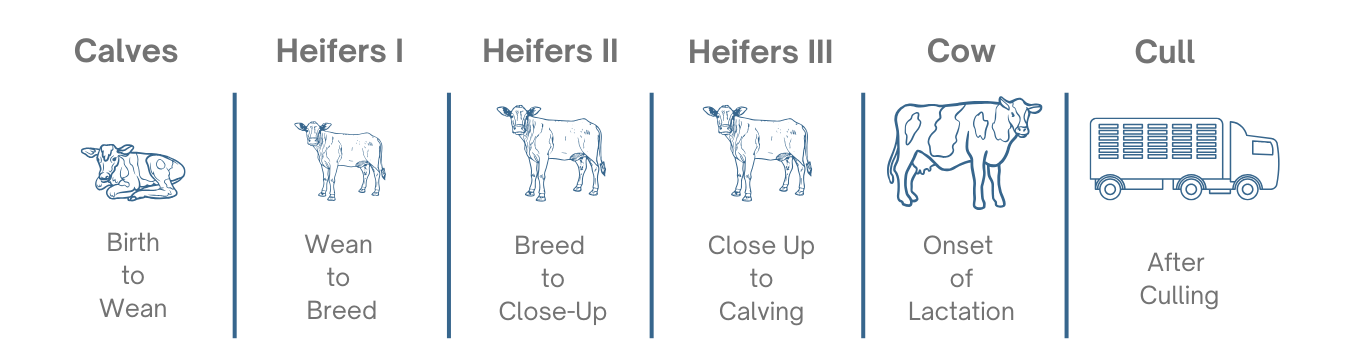
\includegraphics[width=0.9\textwidth]{resources/animalgroups.png} % Replace with your image file
  \caption{There are 5 life stages from calf to cow and a cull stage as outlined in this figure.}
  
\end{figure}

\textbf{Progression Between Life Stages:} Calves progress to Heifer I when their age reaches the user-defined input for weaning day. Heifer I animals progress to Heifer II animals when their age reaches the user-defined input for breeding start day. Heifer II animals that successfully conceive progress to the Heifer III stage when they are close to calving. Specifically, Heifers II become Heifers III when the number of days left in their pregnancy is equal to the user-defined input for the prefresh days. When a Heifer III animal calves for the first time, she becomes a Cow and will remain a cow for the rest of her life on the RuFaS farm. 

When a Heifer III calves for the first time and becomes a Cow, then that animal will cycle through lactating and non-lactating phases until they are removed from the herd due to a failure to conceive or a user-provided probability for culling within each parity. The methods that determine when a cow will leave the herd are described in detail in the Herd Exits section.

\textbf{Parturition and New Calves: }
When a Heifer III or Cow animal reaches the end of their pregnancy and starts lactating, a new calf animal object is created and assigned a birthweight according to a user-informed random distribution. All male calves are recorded and removed from the farm on day 1 of their life. Female calves remain on the farm determined by an event-based Monte Carlo method informed by the user-defined percent of female calves that are kept. 
\subsection{RuFaS Bodyweight and Growth}

    \paragraph{Introduction} An animal’s bodyweight is initialized at birth according to a user defined normal distribution. Depending on her life stage, her bodyweight is then updated daily by adding their daily growth (commonly referred to as average daily gain), conceptus weight change, and tissue accretion and depletion associated with tissue mobilization to support lactation. The changes associated with each life stage are:
    \begin{itemize}
        \item Calves increase bodyweight by calf specific estimate for daily growth from birth to weaning.
        \item Non-pregnant heifers increase bodyweight by non-pregnant heifer specific estimate for daily growth from weaning until conception.
        \item Pregnant heifers  increase their bodyweight by the pregnant heifer specific estimate for daily growth and an estimate for conceptus growth.
        \item Cows in parity 1 and 2 increase their bodyweight according to a parity and pregnancy status specific estimate for daily growth, an estimate for conceptus growth, and an estimate for body tissue changes that occur in lactation. 
        \item Cows in parities 3 and above change their bodyweight according to estimates for conceptus growth and body tissue changes that occur in lactation.
    \end{itemize}
    
    These methods are further described by \textcite{Li2023}

\textbf{Required User Inputs} 

\renewcommand{\arraystretch}{1.4}
\begin{longtable}{@{} L{4cm} L{6.5cm} L{1.5cm} L{1cm} L{1cm} @{}}
\caption{Below is a summary of the user inputs that are available and their definitions.} \\
\toprule

\multicolumn{1}{c}{\textbf{Variable}} & 
\multicolumn{1}{c}{\textbf{Definition (units)}} & 
\multicolumn{1}{c}{\textbf{Default}} & 
\multicolumn{1}{c}{\textbf{Min}} & 
\multicolumn{1}{c}{\textbf{Max}} \\

\midrule
\endfirsthead

\toprule
\multicolumn{1}{c}{\textbf{Variable}} & 
\multicolumn{1}{c}{\textbf{Definition (units)}} & 
\multicolumn{1}{c}{\textbf{Default}} & 
\multicolumn{1}{c}{\textbf{Min}} & 
\multicolumn{1}{c}{\textbf{Max}} \\
\midrule
\endhead

\bottomrule
\endfoot

\bottomrule
\endlastfoot

birth\_weight\_avg\_ho       & Average Holstein Birth Weight (kg/head)       & 42.9       & 1       & NA \\
birth\_weight\_std\_ho       & Holstein Birth Weight Standard Deviation (kg/head)       & 69       & 0       & NA \\
birth\_weight\_avg\_je       & Average Jersey Birth Weight (kg/head)       & 25.2       & 1       & NA \\
birth\_weight\_std\_je       & Jersey Birth Weight Standard Deviation (kg/head)       & 4.4       & 0       & NA \\
mature\_body\_weight\_avg       & The average mature body weight of cows (kg/head)      & 740.1       & 0       & NA \\
mature\_body\_weight\_std       & The standard deviation of mature body weight of cows  (kg/head)    & 73.5       & 0       & NA \\
wean\_day       &  The days of age at which calves are fully weaned from milk or milk replacer (days)     & 60       & 0       & NA \\
target\_heifer\_preg\_day       & The target age (in days) for heifers to become pregnant - for adjusting heifer body weight (days)      & 420       & NA      & NA \\
\end{longtable}

\textbf{Expected Outputs} 
\begin{itemize}
    \item herd\_statistics.avg\_cow\_body\_weight (kg): the daily average bodyweight of all cows in the herd 
    \item Pen\_[pen ID]\_[pen animal combination].avg\_BW (kg): the daily average bodyweight of all animals in each pen
    \item sold\_weight (kg)
\end{itemize}
\vspace{0.5cm}

    \paragraph{Methodology} 
    
    Most methods determining the bodyweight of animals in RuFaS are implemented in growth.py. 
    
    The function evaluate\_body\_weight\_change in growth.py calls the appropriate bodyweight change functions for each animal depending on their life stage and sums the appropriate changes into a single variable called daily\_growth. 

    After setting the daily bodyweight change in the daily\_growth variable, the evaluate\_body\_weight\_change function updates each animal's bodyweight by adding it to the current body\_weight. Thus for all animals, the final updated body\_weight is set as:
    \vspace{0.25cm}
    
    \begin{center}
    \(\text{body\_weight}_{\text{updated}} = \text{body\_weight}_{\text{current}} + \text{daily\_growth}\)        
    \end{center}

\begin{itemize}
    \item \textbf{Calf Birth Weight} is assigned in reproduction.py using a random draw from a truncated normal distribution based on user inputs for the breed-specific average and standard deviation of the birthweight. The distribution is truncated at +/- 2 SD from the mean to prevent extremely small or large calves. 
    \vspace{0.5cm}
    
\begin{center}
    \(Birth\ Weight = Random\ N\ (average\_birth\_weight\_by\_breed,\ std\_std\_birth\_by\_breed)\) 
    
    *Note - truncated at 2 standard deviations
\end{center}
    \vspace{0.5cm}
    
    {\raggedleft \textbf{[AN.BWT.6]}\par}
    \vspace{0.5cm}

    \item \textbf{Calf Growth} Calves are assumed to double their weight between birth and weaning based on recommendations in the \cite{nrc2001}. Thus the target average daily gain is estimated as:
    \vspace{0.5cm}

\begin{center}
    
    \(target\_average\_daily\_gain = \frac{birth\ weight}{wean\ day}\)
    
\end{center}
    \vspace{0.5cm}
    
    {\raggedleft \textbf{[AN.BWT.7]}\par}
    \vspace{0.5cm}
    
    \item \textbf{Non Pregnant Heifer Growth} The daily growth for non-pregnant heifers is estimated through an average daily gain to reach 55\% of their manure bodyweight by the time they are pregnant. Because the actual age at pregnancy is not known, a user input for the target\_heifer\_preg\_day is used to estimate the target average daily growth or ADG. A minimum daily growth rate of 0.5 kg/d is enforced so if the estimated daily\_growth is less than 0.5 kg/d, the minimum value is used. 
    \vspace{0.5cm}
    
 \begin{center}
    \(target\_average\_daily\_gain = min(\frac{0.55×MSBW-SBW}{abs(target heifer pregnant age-age)}\),0.5)
\end{center}
    \vspace{0.5cm}
    
    {\raggedleft \textbf{[AN.BWT.8]}\par}
    \vspace{0.5cm}
    
    Where MSBW is mature shrunk bodyweight (0.96 x mature bodyweight) and SBW is shrunk bodyweight (0.96 x bodyweight)
    
    \item \textbf{Pregnant Heifer Growth} Heifers are targeted to grow to 82\% of their mature body weight by the time of their first calving. A gestation length is set at conception. The ADG of pregnant heifers is calculated based on the target heifer's body weight, gestation length, and days in pregnancy. The gestation length for each animal is set at conception by calculate\_gestation\_length in reproduction.py.
    \vspace{0.5cm}
 
\begin{center}
    \(target\_average\_daily\_gain = \frac{0.82×MSBW-SBW}{gestation length - days in pregnancy}\)
\end{center}
    \vspace{0.5cm}
    
    {\raggedleft \textbf{[AN.BWT.9]}\par}
    
    \item \textbf{Parity 1 and 2 Cow Growth} The daily growth of cows is calculated based on the target of reaching 92\% of the mature body weight by the end of the 1st lactation, and full mature body weight at the end of the 2nd lactation. Before pregnancy, the daily growth is estimated based on the calving interval and during pregnancy the daily growth is calculated based on days until calving. 
    \vspace{0.5cm}
    
    \paragraph{Parity 1 Animals:}
    \vspace{0.25cm}
    
    \textbf{\textit{If not pregnant:}}
    \vspace{0.5cm}
    
\begin{center}
    \(target\_average\_daily\_gain = \frac{(0.92-0.82) × MSBW}{calving\_interval}\)
\end{center}
    \vspace{0.5cm}
    
    {\raggedleft \textbf{[AN.BWT.10]}\par}
    \vspace{0.5cm}
    
    \textbf{\textit{If pregnant:}}
    \vspace{0.5cm}
    
\begin{center}
    \(target\_average\_daily\_gain = \frac{0.92 × MSBW - bodyweight}{gestation\_length - DIP}\)
\end{center}
    \vspace{0.5cm}
    
    {\raggedleft \textbf{[AN.BWT.11]}\par}
    \vspace{0.5cm}

    \paragraph{Parity 2 Animals}
    \vspace{0.5cm}

    
    \textbf{\textit{If not pregnant:}}
    \vspace{0.5cm}
    
\begin{center}
    \(target\_average\_daily\_gain = \frac{(1 - 0.92) × MSBW}{calving\_interval}\)
\end{center}
    \vspace{0.5cm}
    
    {\raggedleft \textbf{[AN.BWT.12]}\par}
    \vspace{0.5cm}
    
    \textbf{\textit{If pregnant:}}
    \vspace{0.5cm}
    
\begin{center}
    \(target\_average\_daily\_gain = \frac{(MSBW - bodyweight)}{gestation\_length - DIP}\)
\end{center}
    \vspace{0.5cm}
    
    {\raggedleft \textbf{[AN.BWT.13]}\par}
    \vspace{0.5cm}
    
The gestation length for cows is estimated with the same methods that are used for heifers and the calving interval is set either as the average herd calving interval or the animal’s own calving interval which is calculated as the age at her second calving minus her age at first calving as part of the daily\_reproduction\_update in animal.py.

    \item \textbf{Conceptus Growth} is estimated the same way for both heifers and cows using a non-linear model for animals that are greater than 50 days in pregnancy based on the methods developed by \textcite{Korver1985}. 
    \vspace{0.25cm}
    
    If the heifer or cow days in pregnancy is greater than 50  and less than the gestation length:

    First the expected total conceptus weight is estimated using an empirical equation based on the calf birth weight and the gestation length:
     \vspace{0.5cm}
     
\begin{center}
    \(conceptus\_total\_weight = (0.0148\ *\ gestation\_length) × calf\_birth\_weight\)
\end{center}
    \vspace{0.5cm}
    
    {\raggedleft \textbf{[AN.BWT.14]}\par}
    \vspace{0.5cm}
    
    Then an animal specific conceptus parameter is calculated:
     \vspace{0.5cm}
     
\begin{center}
    \(conceptus\_parameter = \frac{total\_conceptus\_weight^\frac{1}{3}}{gestation\_length - 50}\)
\end{center}
    \vspace{0.5cm}
    
    {\raggedleft \textbf{[AN.BWT.15]}\par}
    \vspace{0.5cm}
    
    Finally, the conceptus growth is estimated as:
     \vspace{0.5cm}
     
\begin{center}
    \(conceptus\_growth = 3\ *\ conceptus\ parameter^3\ *\ (DIP - 50)^2\)
\end{center}
    \vspace{0.5cm}
    
    {\raggedleft \textbf{[AN.BWT.16]}\par}
    \vspace{0.5cm}
    
    When days\_in\_pregnancy = gestation\_length and the animal calves, then conceptus growth is set to the negative value of the current conceptus\_weight such that the weight of the calf and placenta are subtracted from the cow’s bodyweight when her bodyweight is updated.
        \vspace{0.5cm}
        
\begin{center}
    \(conceptus\_growth = conceptus\_weight\)
\end{center}
    \vspace{0.5cm}
    
    {\raggedleft \textbf{[AN.BWT.17]}\par}
    \vspace{0.5cm}
    
    \item \textbf{Tissue Change Due to Lactation} Lactation related tissue changes are estimated by a non-linear model presented by \textcite{Galvao2013} that estimates the daily tissue mobilized during lactation. 
     \vspace{0.5cm}
     
\begin{center}
    \(bodyweight\_tissue\_change = \frac{P1}{P2}\ *\ exp\ (1\ -\ \frac{DIM}{P2})\ +\ DIM\ x\ exp\ (1\ -\ \frac{DIM}{P2})\)
\end{center}
    \vspace{0.5cm}
    
    {\raggedleft \textbf{[AN.BWT.18]}\par}
    \vspace{0.5cm}
    
    Where P\textsubscript{1} and P\textsubscript{2} are parameters with distinct values for primiparous and multiparous cows:

    \begin{table}[h!]
    \centering
    \renewcommand{\arraystretch}{1.3}

    \begin{tabular}{@{} L{3cm} L{3cm} L{3cm} @{}}
    \toprule
    \multicolumn{1}{c}{\textbf{Parameter}} & 
    \multicolumn{1}{c}{\textbf{Primiparous}} & 
    \multicolumn{1}{c}{\textbf{Multiparous}} \\
    \midrule
    P\textsubscript{1}    & 20   & 65 \\
    P\textsubscript{2}    & 40 & 70 \\
    \bottomrule
    \end{tabular}
    \end{table}


    During the dry period, the net tissue change is assumed to be restored during the dry period. The net tissue change is estimated on the last day of lactation as: 
    \vspace{0.5cm}
    
    \begin{center}
    \(tissue\_changed = P_1\ *\ \frac{DIMlast}{P_2}\ *\ exp\ (1\ -\ \frac{DIMlast}{P_2})\ +\ DIM\ *\ exp\ (1\ -\ \frac{DIM}{P_2})\)
    \end{center}
    \vspace{0.5cm}
    
    {\raggedleft \textbf{[AN.BWT.19]}\par}
         \vspace{0.5cm}
         
    \begin{center}
    \(bodyweight\_tissue\_change = \frac{tissue\ changed}{gestation\ length\ -\ DIPdry}\)
    \end{center}
    \vspace{0.5cm}
    
    {\raggedleft \textbf{[AN.BWT.20]}\par}
\end{itemize}

 


\subsection{Animal Reproduction} 
 
    \paragraph{Introduction} The reproduction component of the RuFaS model is designed based on reproductive program options recommended by the Dairy Cattle Reproduction Council \parencite{dcrc_protocols} and experts in the field. It offers three pre-defined reproductive program options for nulliparous heifers (estrus detection [ED], timed artificial insemination [TAI], and synchronized estrus detection [Synch-ED]) and three options for lactating cows (ED, TAI, and a combined ED-TAI approach). Users can select appropriate reproductive protocols and specify reproductive performance variables for both nulliparous heifers and lactating cows.
    
    \vspace{0.20cm}This reproduction component simulates key reproductive events, including estrus occurrence, estrus detection, hormone administration, artificial insemination (AI), pregnancy checks, and pregnancy outcomes (abortion or successful delivery). Reproductive culling decisions are also modeled, based on an animal's inability to conceive or sustain a pregnancy. These processes are modeled using Monte Carlo simulations to represent variability in reproductive events.

    \vspace{0.2cm}The simulation generates and tracks detailed reproductive performance metrics at the animal level. These outputs provide insights into estrus detection, synchronization treatments, breeding efficiency, and pregnancy outcomes. The key recorded variables include:
    \begin{itemize}
        \item Estrus Detection (ED) Metrics: Number of days an animal participates in the ED program (ED\_days) and the total estrous events detected (estrus\_count).
        \item Hormonal Treatments: Counts of synchronization protocol injections, including GnRH (GnRH\_injections), PGF (PGF\_injections), and CIDR (CIDR\_injections).
        \item Breeding Interventions: Number of semen straws used (semen\_number) and total AI procedures performed (AI\_times).
        \item Reproductive Efficiency: Time from first breeding attempt to pregnancy confirmation (breeding\_to\_pregnancy\_time) and the interval from calving to confirmed pregnancy (calving\_to\_pregnancy\_time).
        \item Pregnancy Monitoring: Total number of pregnancy checks performed (pregnancy\_diagnoses).
    \end{itemize}

\textbf{Required User Inputs}
\vspace{-0.25cm}


% --- Table 1: Heifer Reproductive Inputs ---
\begin{landscape}
\thispagestyle{empty}
\begin{table}[h!]
\caption{Below are the key user inputs that determine the \textbf{heifer reproductive breeding program} and impact reproductive efficiency and age at first calving.}
\centering
\renewcommand{\arraystretch}{1.4}
\begin{tabular}{@{} L{3.5cm} L{3cm} L{8cm} C{2cm} C{2cm} C{2cm} @{}}
\toprule
\textbf{Section} & \textbf{Variable} & \textbf{Definition} & \textbf{Default} & \textbf{Min} & \textbf{Max} \\
\midrule

\multirow{3}{*}{\textbf{management\_decisions}} 
 & breeding\_start\_day\_h & Age when RuFaS initiates estrous protocol (days) & - & 380 & 0 \\
 & heifer\_repro\_method & TAI (Timed AI), ED (Estrus Detection), Synch-ED (Synchronized ED) & TAI & \multicolumn{2}{C{6cm}}{TAI, ED, Synch-ED} \\
 & heifer\_repro\_cull\_time & Age when a heifer is culled if not pregnant (days) & - & 500 & 0 \\
\cmidrule(lr){1-6}

\multirow{5}{*}{\textbf{farm\_level\_heifers}} 
 & estrus\_detection\_rate & Proportion of estrus detected in ED protocol & 0.9 & 0 & 1 \\
 & estrus\_conception\_rate & Conception rate in ED protocol & 0.6 & 0 & 1 \\
 & repro\_sub\_protocol & Hormone protocol used; varies by method (e.g., 5dCG2P, CP, N/A) & 5dCG2P & \multicolumn{2}{C{6cm}}{5dCG2P, 5dCGP, 2P, CP, N/A} \\
 & conception\_rate & Conception rate for sub-protocol & 0.6 & 0 & 1 \\
 & estrus\_detection\_rate & Detection rate in sub-protocol & 0.6 & 0 & 1 \\
\bottomrule
\end{tabular}
\end{table}
\end{landscape}


% --- Table 2: Cow Reproductive Inputs (longtable) ---
\begin{landscape}
\thispagestyle{empty}
\renewcommand{\arraystretch}{1.4}

\begin{longtable}{@{} L{3.5cm} L{3cm} L{8cm} C{2cm} C{2cm} C{2cm} @{}}
\caption{The following inputs determine reproductive efficiency of cows and influence culling, calving interval, and calf output.} \\
\toprule
\textbf{Section} & \textbf{Variable} & \textbf{Definition} & \textbf{Default} & \textbf{Min} & \textbf{Max} \\
\midrule
\endfirsthead

\multicolumn{6}{@{}l}{\textit{Table continued from previous page}} \\
\toprule
\textbf{Section} & \textbf{Variable} & \textbf{Definition} & \textbf{Default} & \textbf{Min} & \textbf{Max} \\
\midrule
\endhead

\midrule
\multicolumn{6}{@{}r@{}}{\textit{Continued on next page}} \\
\endfoot

\bottomrule
\endlastfoot

\multirow{2}{*}{\textbf{management\_decisions}} 
& cow\_repro\_method & TAI, ED, ED-TAI protocols & TAI & \multicolumn{2}{C{6cm}}{TAI, ED, ED-TAI} \\
& do\_not\_breed\_time & Days after calving to stop breeding if not pregnant & 185 & 0 & - \\
\cmidrule(lr){1-6}

\multirow{2}{*}{\textbf{farm\_level}} 
& voluntary\_waiting \_period & Days before breeding starts for ED/ED-TAI; ignored in TAI & 50 & 0 & - \\
& estrus\_detection \_protocol & Estrous protocol type & Double OvSynch & \multicolumn{2}{C{6cm}}{Double OvSynch, PreSynch, G6G, None} \\
\cmidrule(lr){1-6}

\multirow{3}{*}{\textbf{farm\_level\_cows}} 
& estrus\_conception\_rate & Conception rate for ED/ED-TAI & 0.5 & 0 & - \\
& presynch\_program & Presynch method used in TAI & OvSynch 56 & \multicolumn{2}{C{6cm}}{OvSynch 48, OvSynch 56, CoSynch 72, 5d CoSynch, None} \\
& presynch\_program \_start\_day & Day of first hormone injection for presynch & 70 & 0 & - \\
& ovsynch\_program & OvSynch protocol used in TAI or ED-TAI & 0.6 & 0 & 1 \\
& ovsynch\_program \_start\_day & Start day for OvSynch protocol & TAIafterPD & \multicolumn{2}{C{6cm}}{TAIafterPD, TAIbeforePD, PGFatPD, None} \\
& ovsynch\_program \_conception\_rate & Conception rate for OvSynch program & - & - & - \\
& resynch\_program & Resynch protocol around pregnancy check & - & - & - \\
\end{longtable}

\vspace{-0.3cm}
{\footnotesize\textit{NOTE:} Anytime an insemination is performed after an OvSynch program, the conception rate will be changed to the ovsynch\_program\_conception\_rate.}
\end{landscape}


% --- Table 3: Conception Rate Modifiers ---
\begin{landscape}
\thispagestyle{empty}
\begin{table}[h!]
\caption{The following inputs can be used to determine if there is a \textbf{decrease in the conception rate} with parity and rebreeding attempts.}
\centering
\renewcommand{\arraystretch}{1.4}
\begin{tabular}{@{} L{2cm} L{5cm} L{8cm} C{2cm} C{2cm} C{2cm} @{}}
\toprule
\textbf{Section} & \textbf{Variable} & \textbf{Definition} & \textbf{Default} & \textbf{Min} & \textbf{Max} \\
\midrule

\multirow{3}{*}{\textbf{farm\_level}} 
& conception\_rate\_decrease & Percent decrease per breeding attempt after first & 0.026 & 0.1 & 0 \\
& decrease\_conception\_rate \_in\_rebreeding & Whether to decrease rate with rebreeding & FALSE & - & - \\
& decrease\_conception\_rate \_by\_parity & Whether to decrease rate by parity & FALSE & - & - \\
\bottomrule
\end{tabular}
\end{table}
\end{landscape}









\textbf{Relevant Outputs}

Overall reporting for reproductive measures can be summarized and split into scheduled events and updates on an individual basis for heifers and cows. 

These include: 
\begin{itemize}
    \item Events for Estrus (detection and scheduling)
    \item Hormone Administration
    \item Artificial Insemination (AI) (scheduling and status)
    \item Pregnancy Checks and Status
    \item Days Carry Calf
    \item Abortion Events
    \item Updates to Lactation
    \item Updates to Estrous
    \item Updates to Pregnancy
    \item Updates to Reproductive Status or Culling Decisions
    \item Updates to Protocols
\end{itemize}

    \paragraph{Methodology} 
    \textbf{\textit{Heifer Breeding}}
    \vspace{0.2cm}
    
    \textbf{Heifer II} - The heiferII\_reproduction\_update represents the breeding-eligible heifer stage, beginning when the animal enters a reproductive management program and ending when she reaches a user-defined day in pregnancy that marks the start of the pre-fresh period (prefresh\_day). The breeding process follows the assigned reproductive management program and is simulated as described below (Figure 2). Each program includes a user-defined conception rate (conception\_rate), determining the probability of pregnancy initiation at the time of insemination. 
    \begin{figure}[H] % The 'p' option places the figure on a page by itself
  \centering
  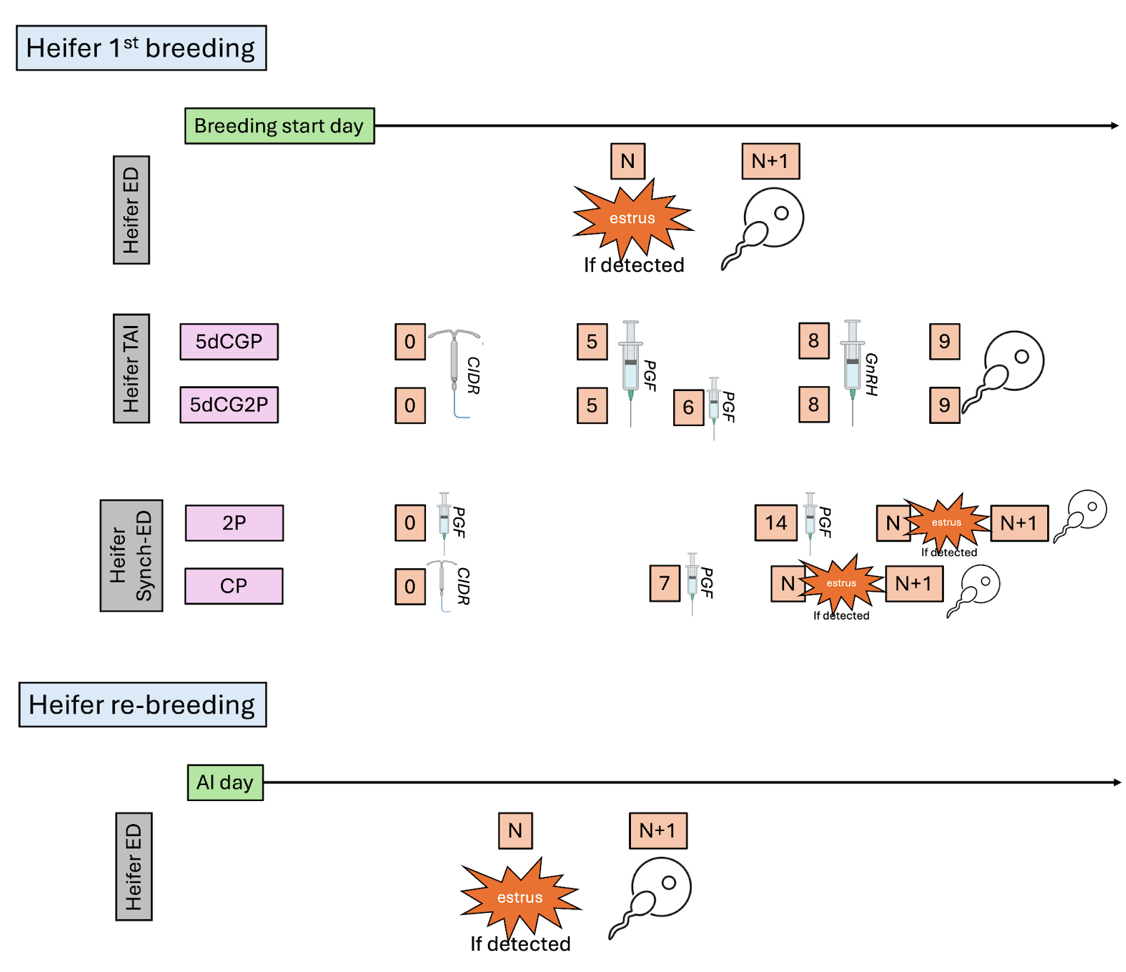
\includegraphics[width=0.7\textwidth]{resources/repromethod.png} % Replace with your image file
  \caption{This is a high level schematic to illustrate the  methodology behind the heifer breeding and re-breeding in RuFaS Animal Module.}
  
\end{figure}
    Pregnancy diagnosis and reconfirmation occur after each insemination [heifer\_pregnancy\_update]. If a heifer remains nonpregnant beyond a user-defined age threshold (heifer\_repro\_cull\_time, e.g., 500 days), she is culled due to reproductive failure. At a user-defined day in pregnancy (prefresh\_day, e.g., one month before calving), the animal either transitions to the Heifer III stage or is sold as a replacement heifer. 
    \vspace{0.2cm}
    
    The first-service reproductive management strategy for a heifer follows one of three strategies and are described in more detail below: estrus detection (ED), synchronized estrus detection (Synch-ED), or timed artificial insemination (TAI).
    \begin{enumerate}
        \item \textbf{ED [execute\_heifer\_ed\_protocol]}: The ED strategy simulates spontaneous estrous cycles. Estrous cycle length is determined using a random draw from a normal distribution \parencite{devries2006}. On the day of estrus predicted by the model, a random draw from a uniform distribution U(0,1) is compared with the estrus detection rate (estrus\_detection\_rate). If the drawn value is lower than the detection rate, AI is scheduled on that day. If estrus is not detected, the next estrus event is scheduled based on the normal estrous cycle. On the scheduled AI day, pregnancy success is determined using a random draw from a uniform distribution U(0,1), which is compared against the conception rate (conception\_rate).
        \item \textbf {Synch-ED [execute\_heifer\_synch\_ed\_protocol]}: In the Synch-ED strategy, hormonal treatment dates are scheduled according to the assigned program (repro\_sub\_protocol, 2P or CP), and estrus is simulated based on a program-specific estrous cycle following the hormonal treatment. Estrus detection and AI scheduling follow the same procedure as in the ED program. 
        \item \textbf{TAI [execute\_heifer\_tai\_protocol]}: The TAI strategy simulates hormonal treatments administered on scheduled days from the start of the synchronization protocol. The timing of treatments and AI is modeled according to the assigned specific program (5dCGP or 5dCG2P) defined as a sub-protocol in the user inputs (repro\_sub\_protocol). On the scheduled AI day, pregnancy success is determined using a random draw from a uniform distribution U(0,1), which is compared against the conception rate (conception\_rate).
    \end{enumerate}
    For all heifers who fail to conceive after the first insemination or experience pregnancy loss [open\_heifer], the ED strategy is applied for subsequent breeding attempts.
    
    \textbf{\textit{Cow Breeding}} The breeding process for cows begins after calving and the voluntary waiting period (VWP), following one of three reproductive management strategies available for cows which are similar to those described in the heifer section and are pictured in Figure 3: ED, TAI, or ED-TAI. The program assigned to a cow determines the timing of insemination and the probability of pregnancy initiation.
    \vspace{-0.5cm}

\begin{figure}[p]
  \centering
  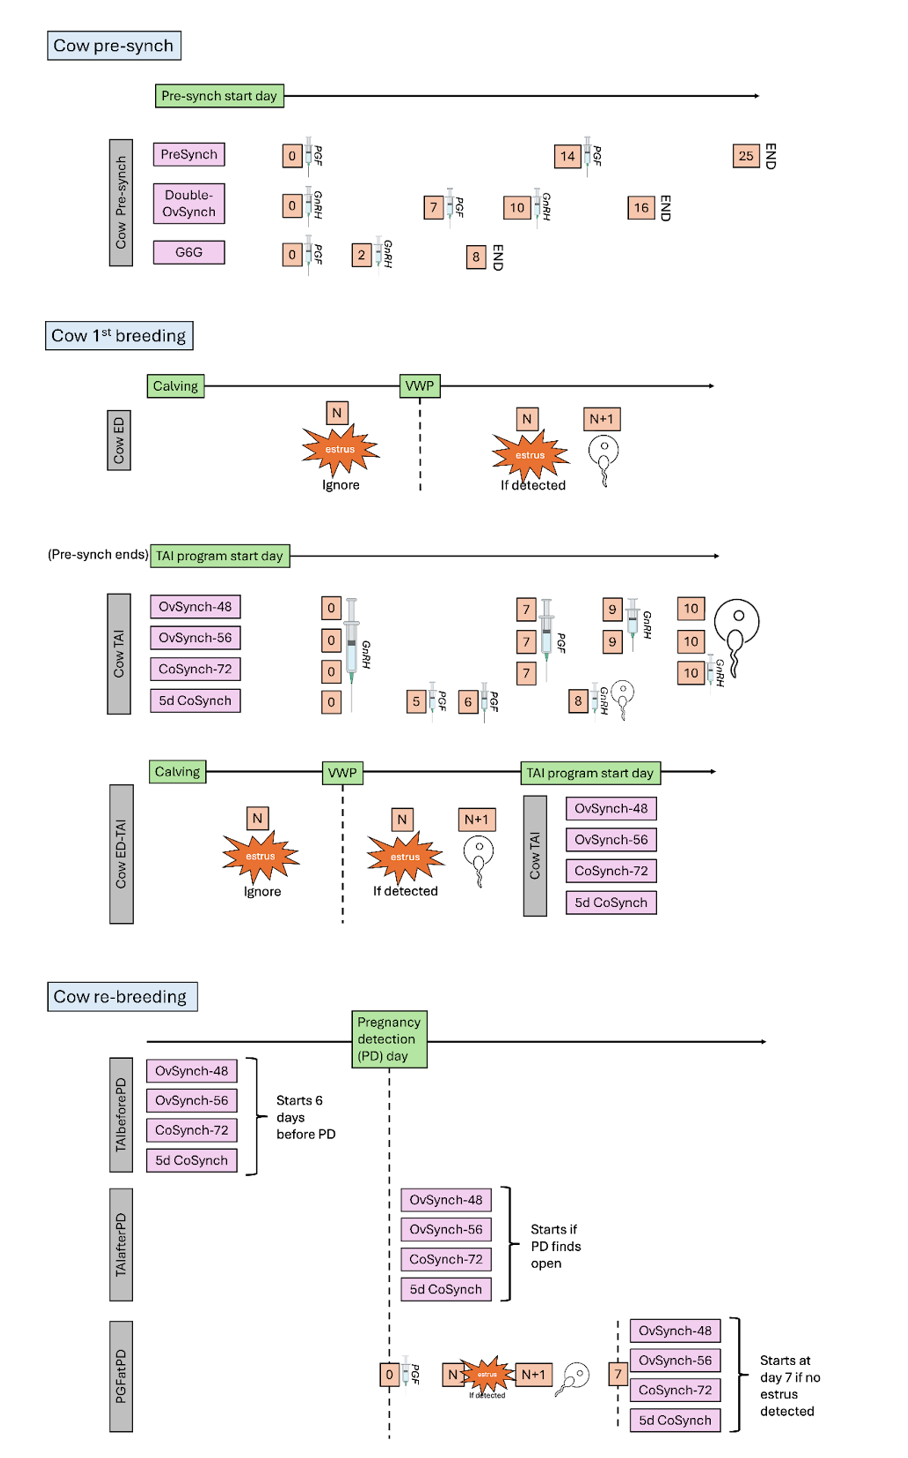
\includegraphics[width=0.75\textwidth]{resources/cowbreedmethod.png}
  \caption{This is a high level schematic to illustrate the methodology behind the cow breeding and re-breeding in RuFaS Animal Module.}

\end{figure}


    \begin{itemize}
        \item \textbf{ED [execute\_cow\_ed\_protocol]}: In the ED strategy, spontaneous estrous cycles are simulated. The first estrous cycle after calving is determined on the calving date using a random draw from a normal distribution with user-specified mean and standard deviation \parencite{kalantari2015using}. The subsequent estrous cycles are modeled similarly. If the scheduled estrus occurs before the VWP, the estrus is ignored. If the scheduled estrus occurs after the VWP, estrus detection is simulated following the same procedure as in the heifer ED strategy - a random draw from a uniform distribution U(0,1) is compared with the estrus detection rate (estrus\_detection\_rate). If the drawn value is lower than the detection rate, AI is scheduled on that day. If estrus is not detected, the next estrus event is scheduled according to the estrous cycle length. On the scheduled AI day, pregnancy success is determined using a random draw from a uniform distribution U(0,1), which is compared against the conception rate (ED\_conception\_rate). 
        \item \textbf{TAI [execute\_cow\_tai\_protocol]}: The TAI strategy simulates hormonal treatments administered on scheduled days according to the assigned synchronization protocol after the start of the breeding date (ovsynch\_program\_start\_day). The timing of treatments and AI follow the predefined protocols (ovsynch\_program, OvSynch-48, OvSynch-56, CoSynch-72, or 5d CoSynch). These protocols can be implemented alone or in combination with presynchronization protocols (presynch\_program, PreSynch, Double OvSynch, or G6G). On the scheduled AI day, pregnancy success is determined using a random draw from a uniform distribution U(0,1), compared against the conception rate.
        \item \textbf{ED-TAI [execute\_cow\_ed\_tai\_protocol]}: The ED-TAI strategy integrates ED with TAI-based synchronization programs. Estrus detection is simulated before TAI begins. If estrus is detected after VWP (voluntary\_waiting\_period) and before the initiation of the TAI (ovsynch\_program\_start\_day), AI is scheduled according to the estrus detection protocol. If no estrus is detected, the cow follows the TAI protocol for insemination.
    \end{itemize}

\begin{tcolorbox}[colback=white, colframe=black, title=Important Note]
For rebreedings, cows can be assigned to any of the three rebreeding strategies (resynch\_program, TAIbeforePD, TAIafterPD, or PGFatPD) [open\_cow].
\end{tcolorbox}


    \begin{itemize}
        \item \textbf{TAIbeforePD}: The TAIbeforePD rebreeding strategy initiates a timed AI synchronization protocol before the first pregnancy diagnosis (PD). Cows that are due for pregnancy diagnosis but have not been confirmed pregnant yet start one of the predefined synchronization protocols (OvSynch-48, OvSynch-56, CoSynch-72, or 5-day CoSynch) six days before PD. This approach ensures that if a cow is found open (not pregnant) on PD day, she is already progressing through a synchronization protocol, reducing the waiting period before the next AI attempt.
        \item \textbf{TAIafterPD}: The TAIafterPD rebreeding strategy schedules synchronization for cows that are diagnosed as open on the PD day. If a cow is not pregnant, she is immediately enrolled in one of the available timed AI protocols (OvSynch-48, OvSynch-56, CoSynch-72, or 5-day CoSynch). This ensures timely rebreeding but does not initiate synchronization in advance of PD.
        \item \textbf{PGFatPD}: The PGFatPD rebreeding strategy uses prostaglandin (PGF) administration following PD for open cows to induce estrus. After PGF treatment (day 0), cows are monitored for natural estrus. If estrus is detected, AI is performed accordingly. If no estrus is detected within seven days, the cow is enrolled in a timed AI protocol (OvSynch-48, OvSynch-56, CoSynch-72, or 5-day CoSynch) to ensure insemination. This program balances estrus detection with timed AI, allowing for natural breeding opportunities before initiating synchronization.
    \end{itemize}
    
    \vspace{1cm}
    \textbf{\textit{Pregnancy Diagnosis (PD) and Pregnancy Loss}} For both heifers and lactating cows [heifer\_pregnancy\_update, cow\_pregnancy\_update], pregnancy diagnoses are scheduled at three intervals after AI (preg\_check\_day\_1, preg\_check\_day\_2, preg\_check\_day\_3). The default settings simulate the first at 32 d after insemination, which, if confirmed positive for pregnancy, is followed at 60 d and then at 200 d \parencite{wiltbank2016}; however, the number and day of pregnancy checks can be adjusted by the model user according to farm practices. Between AI and three pregnancy checks, pregnancy losses are simulated to occur according to random draws from a U (0,1) compared with thresholds according to the expected pregnancy losses in each of those periods (preg\_loss\_rate\_1, preg\_loss\_rate\_2, preg\_loss\_rate\_3). The default values are 0.02, 0.096, and 0.017 \parencite{wiltbank2016}. Users can adjust these numbers according to their herd performance.  


\textit{On the next page are some important functions for the reproduction section of this document}


\begin{landscape}
% Suppress header/footer for all pages of the longtable
\fancypagestyle{landscapeplain}{
  \fancyhf{} % clear header and footer
  \renewcommand{\headrulewidth}{0pt}
  \renewcommand{\footrulewidth}{0pt}
}

\pagestyle{landscapeplain} % Apply to all pages in this landscape block

% Begin longtable

\thispagestyle{landscapeplain} % <-- Suppress header/footer
\textbf{\hypertarget{animfunct}{\large Reproduction Functions}} 
\vspace{0.2cm}


\renewcommand{\arraystretch}{1.4}
\begin{longtable}{@{} L{3cm}  L{7cm} L{4cm} L{4cm} L{4cm}  @{}}
\caption{Important functions for the reproduction section.} \\
\toprule

\multicolumn{1}{c}{\textbf{Function}} & 
\multicolumn{1}{c}{\textbf{Description}} & 
\multicolumn{1}{c}{\textbf{Parameters}} & 
\multicolumn{1}{c}{\textbf{Input Origins}} & 
\multicolumn{1}{c}{\textbf{Outputs}}  \\

\midrule
\endfirsthead

\toprule
\multicolumn{1}{c}{\textbf{Function}} & 
\multicolumn{1}{c}{\textbf{Description}} & 
\multicolumn{1}{c}{\textbf{Parameters}} & 
\multicolumn{1}{c}{\textbf{Input Origins}} & 
\multicolumn{1}{c}{\textbf{Outputs}}  \\
\midrule
\endhead

\bottomrule
\endfoot

\bottomrule
\endlastfoot

reproduction\_update &  Updates the reproductive status of all animals daily, including estrus occurrence, detection, AI scheduling, pregnancy status, and culling decisions. & day: (int) Current simulation day. animal\_list: (list) List of all animals in the herd. & day: Updated by the simulation engine. animal\_list: Provided as model input, updated dynamically. & Updated reproductive status for all animals in the herd. Scheduled events for estrus, AI, and pregnancy checks. \\
heiferII\_reproduction \_update &  Manages reproduction processes for Heifer II animals, including estrus detection, breeding attempts, and pregnancy checks. & heifer: (object) Individual Heifer II animal. & heifer: Passed from the herd's current Heifer II group. & Updated estrus, AI status, and pregnancy details for the heifer. \\
cow\_reproduction \_update &  Handles reproduction for lactating cows, including estrus detection, AI, and transitioning reproductive status. & cow: (object) Individual cow object. day: (int) Current simulation day. & cow: Passed from the herd's lactating group. day: Updated by the simulation engine. & Updated estrus, AI, pregnancy status, and culling decisions for the cow. \\
cow\_give\_birth &  Manages calving events, updates the reproductive status, and initializes the lactation process. & cow: (object) Individual cow object. day: (int) Current simulation day. & cow: Passed from the pregnant group. day: Updated by the simulation engine. & Updated lactation and reproductive status for the cow. \\
execute\_heifer \_ed\_protocol &  Executes the estrus detection protocol for heifers, simulating natural estrus occurrence and detection probability. & heifer: (object) Individual Heifer II animal. day: (int) Current simulation day. & heifer: Passed dynamically during estrus updates. day: Updated by the simulation engine. & Estrus detection and AI scheduling for the heifer. \\
execute\_heifer \_tai\_protocol &  Manages the TAI protocol for heifers, simulating hormone administration and AI scheduling. & heifer: (object) Individual Heifer II animal. protocol: (dict) User-defined TAI protocol details. & heifer: Passed dynamically during protocol execution. protocol: Provided as user input. & AI scheduling and protocol updates for the heifer. \\
execute\_heifer \_synch\_ed\_protocol &  Executes synchronized estrus detection protocol for heifers, combining hormonal synchronization and estrus detection. & heifer: (object) Individual Heifer II animal. protocol: (dict) User-defined Synch-ED protocol details. & heifer: Passed dynamically during protocol execution. protocol: Provided as user input. & Estrus detection, hormone administration, and AI scheduling for the heifer. \\
open\_heifer &  Handles open status updates for heifers, reassigning protocols or marking for culling if reproduction fails. & heifer: (object) Individual Heifer II animal. & heifer: Passed dynamically during daily updates. & Updated reproduction status or culling decision for the heifer. \\
heifer\_pregnancy \_update &  Updates pregnancy status for heifers, including pregnancy checks and abortion events. & heifer: (object) Individual Heifer II animal. day: (int) Current simulation day. & heifer: Passed dynamically during daily updates. day: Updated by the simulation engine. & Pregnancy status, days in pregnancy, or abortion event for the heifer. \\
execute\_cow \_ed\_protocol &  Executes estrus detection protocol for cows, simulating natural estrus occurrence and detection probability. & cow: (object) Individual cow object. day: (int) Current simulation day. & cow: Passed dynamically during estrus updates. day: Updated by the simulation engine. & Estrus detection and AI scheduling for the cow. \\
execute\_cow \_tai\_protocol &  Manages the TAI protocol for cows, simulating hormone administration and AI scheduling. & cow: (object) Individual cow object. protocol: (dict) User-defined TAI protocol details. & cow: Passed dynamically during protocol execution. protocol: Provided as user input. & AI scheduling and protocol updates for the cow. \\
execute\_cow \_ed\_tai\_protocol &  Executes ED-TAI protocol for cows, combining estrus detection with synchronized TAI scheduling. & cow: (object) Individual cow object. protocol: (dict) User-defined ED-TAI protocol details. & cow: Passed dynamically during protocol execution. protocol: Provided as user input. & Estrus detection, hormone administration, and AI scheduling for the cow. \\
cow\_pregnancy \_update &  Updates pregnancy status for cows, including pregnancy checks and abortion events. & cow: (object) Individual cow object. day: (int) Current simulation day. & cow: Passed dynamically during daily updates. day: Updated by the simulation engine. & Pregnancy status, days in pregnancy, or abortion event for the cow. \\
open\_cow &  Handles open status updates for cows, reassigning protocols or marking for culling if reproduction fails. & cow: (object) Individual cow object. & cow: Passed dynamically during daily updates. & Updated reproduction status or culling decision for the cow. \\


\end{longtable}

\vspace{0.5cm}
\end{landscape}


\subsection{Milk Production} 
 
    \paragraph{Introduction} This section describes how RuFaS determines the amount of milk and milk components produced by a particular cow on a particular day. 
    \vspace{0.25cm}
    
    Milk yield is largely determined by lactation curve parameters. Wood’s curve is the only lactation model implemented in RuFaS currently, but there is flexibility to potentially include other models as well. At the beginning of the simulation, the herd is assigned distributions for the Wood’s curve parameters l, m, and n for each parity of cows (see more information in the Lactation Curve section). At the beginning of each new lactation, each cow is assigned a set of parameters for that lactation based on the herd’s distributions for her current parity. 
    \vspace{0.25cm}
    
    When the cow starts lactating, she produces milk from the calving day until dry or culled according to the assigned lactation curve model. Each day, each cow’s milk production is calculated and recorded. Milk production is calculated from the Wood’s curve equation using the given lactation curve parameters and days in milk, and then adjusted by applying random variation and any milk reduction required by other parts of the model. Milk components (protein, fat, and lactose) are calculated based on milk production and percent of each component for each cow. 
    \vspace{0.25cm}
    
    Currently, the only source of milk reduction is if there is no possible ration using the feeds available that would support the baseline level of milk production. Ration formulation is attempted with reduced milk production levels until reaching an acceptable ration (that meets the nutrient requirements for the pen’s average cow) or reaching a threshold (floor) milk production defined by some combination of user inputs and pre-defined constants. 
    



\begin{landscape}
% Suppress header/footer for all pages of the longtable
\fancypagestyle{landscapeplain}{
  \fancyhf{} % clear header and footer
  \renewcommand{\headrulewidth}{0pt}
  \renewcommand{\footrulewidth}{0pt}
}

\pagestyle{landscapeplain} % Apply to all pages in this landscape block

\textbf{ Required User Inputs}
\vspace{0.2cm}


\renewcommand{\arraystretch}{1.4} % More vertical space between rows

\begin{longtable}{@{} L{4cm} L{4cm} p{7cm} C{2cm} C{3cm} C{3cm} @{} }

\caption{The following user inputs are used to estimate customized herd-level lactation curve parameters. See the Methodology section of this document and the Lactation Curve Scientific Documentation for more detail about how these inputs are used with relation to daily milk production.} \\
\toprule
\multicolumn{1}{c}{\textbf{Section}} & 
\multicolumn{1}{c}{\textbf{Variable}} & 
\multicolumn{1}{c}{\textbf{Definition}} & 
\multicolumn{1}{c}{\textbf{Default}} & 
\multicolumn{1}{c}{\textbf{Min}} & 
\multicolumn{1}{c}{\textbf{Max}} \\
\midrule
\endfirsthead

\multicolumn{6}{@{}l}{\textit{Table continued from previous page}} \\
\toprule
\multicolumn{1}{c}{\textbf{Section}} & 
\multicolumn{1}{c}{\textbf{Variable}} & 
\multicolumn{1}{c}{\textbf{Definition}} & 
\multicolumn{1}{c}{\textbf{Default}} & 
\multicolumn{1}{c}{\textbf{Min}} & 
\multicolumn{1}{c}{\textbf{Max}} \\
\midrule
\endhead

\midrule
\multicolumn{6}{@{}r@{}}{\textit{Continued on next page}} \\
\endfoot

\bottomrule
\endlastfoot


\multirow{2}{*}{\textbf{config \_properties }} 
& end\_date & The year and Julian day on which the simulation will end & 2009:100 & - (cutoff at 2006) & – (cutoff at 2016) \\
& FIPS\_county\_code & Unique 5-digit code that represents a specific US county & - & 1000 & 56045 \\
\cmidrule(lr){1-6}

\multirow{3}{*}{\textbf{animal \_properties }} 
& cow\_times\_milked\_per\_day & Number of Milkings (per day) -- The average or most common number of times cows are milked per day (1, 2, or 3 times daily) & 3 & 0 & - \\
& parity\_fractions & Fractions of the milking animal population that are parity 1, 2, and 3 and beyond. The sum of these fractions must be 1.0 & 1: 0.346; 2: 0.272; 3: 0.379 & 1 & 0 \\
& annual\_milk\_yield & The total milk yield generated by the farm in one year (kg). If this information is not available, it can be input as null & null & - & 0 \\
\cmidrule(lr){1-6}
lactation\_properties& milking\_cow\_fraction & Fraction of cows assumed to be in milk at any given time & 0.8365 (305/365) & 1 & 0 \\


\end{longtable}
\vspace{-0.3cm}

\end{landscape}



\begin{landscape}
\thispagestyle{empty}  % Suppress headers and footers only on this page

\renewcommand{\arraystretch}{1.4}
\begin{longtable}{@{} L{4cm} L{4cm} p{7cm} C{2cm} C{3cm} C{3cm} @{}}
\caption{The following inputs are used to determine the milk fat and milk protein percentages for each lactating cow} \\
\toprule
\textbf{Section} & 
\textbf{Variable} & 
\textbf{Definition} & 
\textbf{Default} & 
\textbf{Min} & 
\textbf{Max} \\
\midrule
\endfirsthead

\multicolumn{6}{@{}l}{\textit{Table continued from previous page}} \\
\toprule
\textbf{Section} & 
\textbf{Variable} & 
\textbf{Definition} & 
\textbf{Default} & 
\textbf{Min} & 
\textbf{Max} \\
\midrule
\endhead

\midrule
\multicolumn{6}{@{}r@{}}{\textit{Continued on next page}} \\
\endfoot

\bottomrule
\endlastfoot

\multirow{2}{*}{\textbf{animal\_properties}} 
& milk\_fat\_percent & The average or most common milk fat percentage in cow milk & 3.5 & 0 & \\
& milk\_protein\_percent & The average or most common milk protein percentage in cow milk & 3.2 & 0 & \\

\end{longtable}

\vspace{-0.3cm}


\end{landscape}






\begin{landscape}
\thispagestyle{empty}  % Suppress header and footer on this landscape page

\renewcommand{\arraystretch}{1.4} % More vertical space between rows
\begin{longtable}{@{} L{4cm} L{4cm} p{7cm} C{2cm} C{3cm} C{3cm} @{}}
\caption{The following inputs are used to constrain how much an average cow’s daily milk production will be reduced due to an inadequate ration. See the Methodology section of this document and the Ration Formulation scientific documentation for more detail about how these inputs are used with relation to daily milk production.} \\
\toprule
\multicolumn{1}{c}{\textbf{Section}} & 
\multicolumn{1}{c}{\textbf{Variable}} & 
\multicolumn{1}{c}{\textbf{Definition}} & 
\multicolumn{1}{c}{\textbf{Default}} & 
\multicolumn{1}{c}{\textbf{Min}} & 
\multicolumn{1}{c}{\textbf{Max}} \\
\midrule
\endfirsthead

\multicolumn{6}{@{}l}{\textit{Table continued from previous page}} \\
\toprule
\multicolumn{1}{c}{\textbf{Section}} & 
\multicolumn{1}{c}{\textbf{Variable}} & 
\multicolumn{1}{c}{\textbf{Definition}} & 
\multicolumn{1}{c}{\textbf{Default}} & 
\multicolumn{1}{c}{\textbf{Min}} & 
\multicolumn{1}{c}{\textbf{Max}} \\
\midrule
\endhead

\midrule
\multicolumn{6}{@{}r@{}}{\textit{Continued on next page}} \\
\endfoot

\bottomrule
\endlastfoot

\multirow{2}{*}{\textbf{feed\_properties}} 
& milk\_reduction\_maximum & Allowable amount of milk reduction (kg) when dietary nutrient supply cannot meet animal requirements &     &   0 & 50 \\

& tolerance & Allowable +/- percentage variance in each of the defined ration inclusion percentage values. 

\textit{This variable defaults to 0.0 and currently has no effect due to no implementation of an automatic ration optimizer. RuFaS is hard-coded to use the user-defined ration at this time.}
  & 0 & 0 & 1 \\

\end{longtable}

\end{landscape}



\textbf{Relevant Outputs}
\vspace{-0.25cm}

    \begin{itemize}
        \item report\_life\_cycle\_manager\_data:	
        \begin{itemize}
            \item Information added daily from herd statistics
            \item daily\_milk\_production 
            \item herd\_milk\_fat\_percent
            \item herd\_milk\_fat\_kg
            \item herd\_milk\_protein\_percent 
            \item herd\_milk\_protein\_kg
        \end{itemize}

        \item report\_average\_nutrient\_requirements: 
        \begin{itemize}
            \item Reports the average ration per animal of each pen each time a new ration is formulated 
            \item avg\_milk\_production\_reduction\_pen (kg per animal)
        \end{itemize}
    \end{itemize}


    \paragraph{Methodology}
    \begin{enumerate}

        \item \textbf{\textit{Herd Level Lactation Curve Parameters}} 
        \vspace{0.1cm}
        
        At the beginning of the simulation, the herd is assigned distributions for the lactation curve parameters l, m, and n for each parity of cows. It calculates Wood’s lactation curve parameter mean values by parity, adjusted based on the location, production, management practices, +/- reported milk production of the farm being simulated. 
         \vspace{0.1cm}

         \textit{User Inputs and Constants}
         \vspace{0.1cm}

         The following inputs are used to generate the herd’s values for mean lactation curve parameters by parity. 
            
         \begin{itemize}
             \item year: end\_date in the input config.json. Uses 2016 if the end year is 2016 or later.  
             \item region: assigns the appropriate region based on FIPS\_county\_code entered in the input config.json  
             \item milking frequency: cow\_times\_milk\_per\_day in input animal.json 
             \item parity distribution: parity\_fractions in input animal.json 
             \item annual milk yield (optional): annual\_milk\_yield in animal.json 
             \item Milking\_cow\_fraction: 0.8356 default value 
             \begin{itemize}
                 \item Is in lactation\_curve\_adjustment\_inputs.json 
                 \item Fraction of lactating cows in adult cows, between 0 and 1. 
                 \item Used to calculate adjusted lactation curve parameters to match a herd’s reported annual milk production 
             \end{itemize}
         \end{itemize}
         
         \textit{Parameters and Equations}
         \vspace{0.1cm}

         These are comprehensively outlines in the Lactation Curve Parameters Determination Section.
        \vspace{0.1cm}
        
         LactationCurve.set\_lactation\_parameters() is called by:
         \begin{itemize}
             \item HerdFactory.initialize\_herd() to Animal.setup\_lactation\_curve\_parameters() 
             \item HerdManager.\_init\_() 

         \end{itemize}
        \vspace{0.2cm}
        
        \item \textbf{\textit{Cow Level Lactation Curve Parameters}} 
        \vspace{-0.1cm}
        
        Each cow is assigned a set of parameters for each lactation based on the herd’s distributions of l, m, and n for her current parity. This occurs when a cow is initialized at the beginning of the simulation, when a heiferIII (close-up heifer) transitions into a cow, and each time a cow has a calf. It selects Wood’s curve parameters for the cow for each parameter for each parity from the distributions based on the means calculated for the herd and constant standard deviations.
         \vspace{0.1cm}

         \textit{User Inputs and Constants}
         \vspace{0.1cm}

         No additional inputs to consider. 
         
         \textit{Parameters and Equations}
         \vspace{0.1cm}

        \begin{itemize}
            \item LactationCurve.get\_wood\_parameters() is called by
            \begin{itemize}
                \item Animal.\_initialize\_cow
                \item Animal.daily\_reproduction\_update
                \item Animal.transition\_heiferIII\_to\_cow
            \end{itemize}
            \item Parity groupings are as follows: 1, 2, and 3+ 
            \item Immediately followed in each case by self.milk\_production.set\_wood\_parameters() which assigns the l, m, and n values.
        \end{itemize}
            \vspace{0.25cm}

        \item \textbf{\textit{Daily Milk Production}} 
        \vspace{0.1cm}
        
        Each day, each cow’s milk production is calculated and recorded. Milk production is calculated from the Wood’s curve equation using the given lactation curve parameters and days in milk. The calculated production is then adjusted by applying random variation and any milk reduction required by other parts of the model. 
         \vspace{0.1cm}

         \textit{User Inputs and Constants}
         \vspace{0.1cm}

         No additional inputs to consider but constants are below: 
        \begin{itemize}
            \item DAILY\_MILK\_VARIATION\_MEAN: 0 kg/d
            \item DAILY\_MILK\_VARIATION\_STD\_DEV: 1.0 kg/d 
        \end{itemize}

         \textit{Parameters and Equations}
         \vspace{0.1cm}

    \begin{center}
\(Calculated\ milk\ production = l*t^m *e^{[-nt]}\)
    \end{center}
        \vspace{0.5cm} 
    
            {\raggedleft \textbf{[AN.MLK.9]}\par}
            \vspace{0.2cm}

        \begin{itemize}
            \item l, m, n = lactation curve parameters
            \item t = DIM
        \end{itemize}
        \vspace{0.2cm}

        \begin{tcolorbox}[colback=white, colframe=black, boxrule=0.5pt, arc=3pt, width=\textwidth]
            Adjusted milk production = maximum of (calculated milk production + milk production variance - milk production reduction) or 0.
        \end{tcolorbox}
        \vspace{0.2cm}

        \begin{itemize}
            \item MilkProduction.calculate\_daily\_milk\_production()
            \begin{itemize}
                \item \textbf{Called by} HerdManager.daily\_routines() to Animal.daily\_routines() to MilkProduction.perform\_daily\_milking\_update()
                \item \textbf{Parameters} 
                \begin{itemize}
                    \item Days\_in\_milk: Argument supplied from MilkProductionInputs (updated in Animal.daily\_routines)
                    \item L\_param, m\_param, n\_param: Wood\_l, wood\_m, wood\_n supplied as arguments and assigned to individual on the day of calving via set\_wood\_parameters()
                \end{itemize}
                \item \textbf{Returns} calculated milk yield on the provided day in kg 
            \end{itemize}
            \item MilkProduction.daily\_milk\_produced()
            \begin{itemize}
                \item \textbf{Inputs}
                \begin{itemize}
                    \item \_Daily\_milk\_produced (calculated above) 
                    \item Milk\_production\_variance is generated based on the mean and standard deviation for daily milk variation (stored as constants in AnimalModuleConstants)
                    \item Milk\_production\_reduction 
                \end{itemize}
            \end{itemize}
            \item \textbf{Returns} adjusted\_milk\_production (unless the milk yield calculated above was 0, in which case it returns 0)

        \end{itemize}
            \vspace{0.2cm}


        \item \textbf{\textit{Daily Components Production}} 
        \vspace{0.1cm}
        
        Milk components (true protein, fat, and lactose) are calculated daily based on that day’s milk production and percent of each component. 
        \vspace{0.1cm}
        
         \textit{User Inputs and Constants}
         \vspace{0.1cm}

         \begin{itemize}
             \item milk\_fat\_percent – single constant value for all cows in the herd 
             \item milk\_protein\_percent – single constant value for all cows in the herd 
             \item AnimalModuleConstants.MILK\_LACTOSE, current value 4.85

         \end{itemize}

         \textit{Parameters and Equations}
         \vspace{0.1cm}

        \begin{itemize}
            \item \(Daily\ nutrient\ amount\ in\ milk = milk\ production * nutrient\ percentage * 0.01\)
            \item MilkProduction.\_calculate\_nutrient\_content()
            \begin{itemize}
                \item \textbf{Called by} HerdManager.daily\_routines() to Animal.daily\_routines() to MilkProduction.perform\_daily\_milking\_update()
                \item \textbf{Parameters} 
                \begin{itemize}
                    \item Days\_milk\_produced as calculated in the Daily Milk Production section above
                    \item Nutrient\_percentage: cow’s percent true protein, fat, or lactose for each of the respective calculations
                \end{itemize}
                \item \textbf{Returns} Amount of a given nutrient in milk in kg
            \end{itemize}
        \end{itemize}
         
        \begin{tcolorbox}[colback=white, colframe=black, boxrule=0.5pt, arc=3pt, width=\textwidth]
            Please note that currently, true protein is the only milk protein currently used by the model. .
        \end{tcolorbox}

        \item \textbf{\textit{Milk Production and Reduction}} \hypertarget{myprodred}{ }
        \vspace{0.1cm}
        
        Currently, the only source of milk reduction is if there is no possible ration using the feeds available that would support the baseline level of milk production. 
        
        Each time the ration is formulated, the nutrition requirements of the pen are calculated and used to determine the ration given to each animal. The ration is checked against the nutrition requirements of the pen. If the pen contains lactating cows and the ration does not meet the average cow’s requirements, then each cow’s milk production is reduced until one of three conditions is met: 
        \begin{itemize}
            \item The ration meets the animal’s requirement (i.e. no additional reduction).
            \item The milk production of every animal is reduced by the maximum allowed (a user-defined value with default of 0.5 kg/head/d). Then the final ration and milk reduction values are used.
            \item The average milk production of the pen falls below the minimum allowable average milk production. Then the final ration and milk reduction values are used.
        \end{itemize}
        \vspace{0.2cm}
        

        \begin{figure}[H] % The 'p' option places the figure on a page by itself
            \centering
            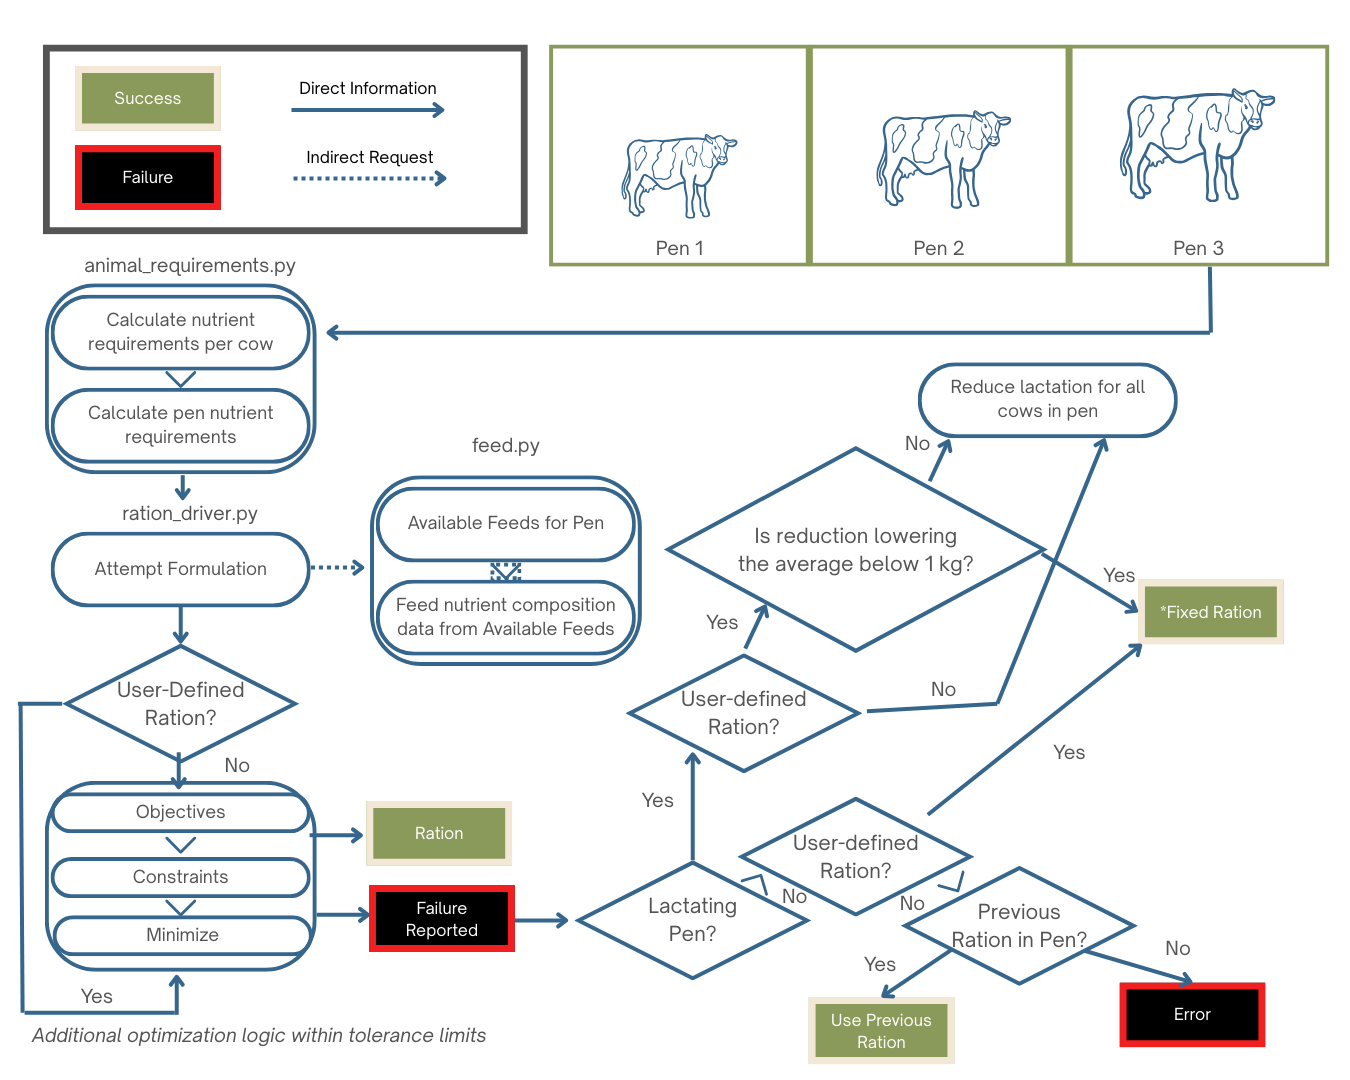
\includegraphics[width=0.9\textwidth]{resources/milkrationform.png} % Replace with your image file
            \caption{A schematic illustrating the flow of milk reduction in ration formulation logic.}
        \end{figure}
        \vspace{0.2cm}

         \textit{User Inputs and Constants}
         \vspace{0.1cm}

         \begin{itemize}
             \item Milk\_reduction\_maximum: Allowable amount of milk reduction (kg) when dietary nutrient supply cannot meet animal requirements 
             \item Tolerance: Allowable +/- percentage variance in each of the defined ration inclusion percentage values. This variable is default to 0.0 and it currently has no effect due to no implementation of automatic ration optimizer. 
            \item Milk\_reduction\_kg is set to 0.25 kg: Milk reduction amount for each failed ration attempt, kg. 
            \item Minimum\_avg\_pen\_milk is set to 15 kg: Minimum allowable average milk production, for a given pen, as used in ration formulation, kg/animal
         \end{itemize}

         \textit{Parameters and Equations}
         \vspace{0.1cm}

        \begin{itemize}
            \item Pen.reduce\_milk\_production()
            \begin{itemize}
                \item \textbf{Called by} Pen.use\_user\_defined\_ration() when NutritionEvaluator determines that the ration is inadequate to support milk production
                \item Attempts to reduce the milk production of all animals in the pen; returns False if all animals have already reached their maximum 
            \end{itemize}
            \item Animal.reduce\_milk\_production() 
            \begin{itemize}
                \item \textbf{Called by} Pen.reduce\_milk\_production for each animal in the pen 
                \item Attempts to reduce milk production of an animal in a pen; returns True if reduction was successful and False otherwise. When reduction is successful, increments milk\_production\_reduction by the value 
            \end{itemize}
        \end{itemize}


        \begin{tcolorbox}[colback=white, colframe=black, boxrule=0.5pt, arc=3pt, width=\textwidth]
            Currently, all cows in a pen will have the same milk reduction amount. This function allows future flexibility if desired to have individual reductions rather than applying the average..
        \end{tcolorbox}


        \item \textbf{\textit{Starting and Ending Lactation}} 
        \vspace{0.1cm}
    
    \textbf{Starting Lactation [Animal.transition\_heiferIII\_to\_cow]}: When a heifer reaches the point where her days pregnant is equal to gestation length, she is transitioned to a lactating cow and configuration data for a newborn calf is returned. 
    
    
    \textbf{[Reproduction.cow\_give\_birth]} and \textbf{[Animal.daily\_reproduction\_update]} When a cow’s days pregnant is equal to gestation length, she gives birth and a newborn calf is born. Her parity is incremented plus one, her days in milk is reset to 1, and she is assigned new Wood’s curve parameters for the new lactation. 
    \vspace{0.5cm}




        \begin{tcolorbox}[colback=white, colframe=black, boxrule=0.5pt, arc=3pt, width=\textwidth]
            For more information, refer to the Reproduction section of this document.
        \end{tcolorbox}
        \vspace{0.2cm}
    
    \textbf{Ending Lactation [ MilkProduction.perform\_daily\_milking\_update]}: When a cow’s days pregnant is equal to her dry off days of pregnancy, her milk production and days in milk are set to 0 and remain there until completing her gestation. Cows with days\_in\_milk = 0 are considered not to be milking and do not have any milk production values calculated. 
    \vspace{0.2cm}
            
        \begin{tcolorbox}[colback=white, colframe=black, boxrule=0.5pt, arc=3pt, width=\textwidth]
            For more details on milk changes and reductions, go to the Milk Production and Reduction portion of this section. . 
        \end{tcolorbox}
    
   
    \end{enumerate}

 
\subsection{Lactation Curve: Parameters and Definitions} 
 
    \paragraph{Introduction} The Lactation Curve Parameter Determination module calculates and adjusts Wood’s lactation curve parameters (l, m, n) based on farm-specific attributes such as geographic location, management practices, and production levels. These parameters shape the milk production curve for cows across different parities (1st, 2nd, 3rd + lactations).
    
    This module is part of the Animal Module and integrates with the Milk Production calculations. The outputs influence various downstream models, including nutrient requirements, manure excretion, and greenhouse gas emission calculations.
    
    The primary class in this module is:
    
    LactationCurve: Manages and adjusts Wood’s lactation curve parameters.

\textbf{\hypertarget{lactcurvreqinputs}{Required User Inputs}}
\vspace{-0.25cm}

% Begin longtable
 The module retrieves input data from simulation configuration files and the Input Manager. These inputs are organized into groups based on their functional roles. Each input is detailed by its parameter name, definition (including units where applicable), and any default values or constraints. There are three categories on inputs that should be considered in this section: 
 \begin{enumerate}
     \item \hyperlink{woodscurve}{Wood's Lactation Curve Base Parameters}
     \item \hyperlink{lactcurvadjust}{Adjustment Factors}
     \item \hyperlink{farmspec305}{Farm Specific 305 d Milk Production}
 \end{enumerate}
 \vspace{0.1cm}

\newpage
\begin{landscape}

% Section header
\textbf{ \hypertarget{woodscurve}{\large Lactation Curve Parameters and Inputs}} 

% Suppress header/footer for all pages of the longtable
\fancypagestyle{landscapeplain}{
  \fancyhf{} % clear header and footer
  \renewcommand{\headrulewidth}{0pt}
  \renewcommand{\footrulewidth}{0pt}
}
\pagestyle{landscapeplain}

\begin{center}
\captionof{table}{Wood's Lactation Curve Base Parameters – These inputs provide the baseline values and variability for Wood’s lactation curve parameters as derived from \textcite{Li2022}.}
\end{center}

\renewcommand{\arraystretch}{1.4} % More vertical space between rows
\begin{longtable}{@{} L{4cm} L{8cm} C{2cm} L{4cm} @{} }

\toprule
\multicolumn{1}{c}{\textbf{Variable}} & 
\multicolumn{1}{c}{\textbf{Definition}} & 
\multicolumn{1}{c}{\textbf{Units}} & 
\multicolumn{1}{c}{\textbf{Default}}  \\
\midrule
\endfirsthead

\multicolumn{4}{@{}l}{\textit{Table continued from previous page}} \\
\toprule
\multicolumn{1}{c}{\textbf{Variable}} & 
\multicolumn{1}{c}{\textbf{Definition}} & 
\multicolumn{1}{c}{\textbf{Units}} & 
\multicolumn{1}{c}{\textbf{Default}}  \\
\midrule
\endhead

\midrule
\multicolumn{4}{@{}r@{}}{\textit{Continued on next page}} \\
\endfoot

\bottomrule
\endlastfoot

parameter\_l\_mean & Baseline value for parameter $l$ of Wood’s lactation curve & Unitless & 19.9 \\
parameter\_m\_mean & Baseline value for parameter $m$ of Wood’s lactation curve & Unitless & 0.247 \\
parameter\_n\_mean & Baseline value for parameter $n$ of Wood’s lactation curve & Unitless & 0.003376 \\
parameter\_l\_std\_dev & Standard deviation for parameter $l$ & Unitless & Parity 1: 0.28; Parity 2: 0.54; Parity 3+: 0.51 \\
parameter\_m\_std\_dev & Standard deviation for parameter $m$ & Unitless & Parity 1: 0.0046; Parity 2: 0.0064; Parity 3+: 0.0060 \\
parameter\_n\_std\_dev & Standard deviation for parameter $n$ & Unitless & Parity 1: 3.77e-5; Parity 2: 5.82e-5; Parity 3+: 5.54e-5 \\

\end{longtable}
\vspace{-0.1cm}

\end{landscape}






\newpage
\begin{landscape}


% Suppress header/footer for all pages of the longtable
\fancypagestyle{landscapeplain}{
  \fancyhf{} % clear header and footer
  \renewcommand{\headrulewidth}{0pt}
  \renewcommand{\footrulewidth}{0pt}
}
\pagestyle{landscapeplain} % Apply to all pages in this landscape block

% Section header
\textbf{\hypertarget{lactcurvadjust}{\large Lactation Curve Adjustment Factors}} 

\begin{center}
    \captionof{table}{Adjustment Factors – These factors adjust the base parameters based on geographical, temporal, management, and parity considerations.}
\end{center}

\renewcommand{\arraystretch}{1.4} % More vertical space between rows
\begin{longtable}{@{} L{4cm} L{8cm} C{2cm} L{4cm} @{} }

\toprule
\multicolumn{1}{c}{\textbf{Variable}} & 
\multicolumn{1}{c}{\textbf{Definition}} & 
\multicolumn{1}{c}{\textbf{Units}} & 
\multicolumn{1}{c}{\textbf{Default}}  \\
\midrule
\endfirsthead

\multicolumn{4}{@{}l}{\textit{Table continued from previous page}} \\
\toprule
\multicolumn{1}{c}{\textbf{Variable}} & 
\multicolumn{1}{c}{\textbf{Definition}} & 
\multicolumn{1}{c}{\textbf{Units}} & 
\multicolumn{1}{c}{\textbf{Default}}  \\
\midrule
\endhead

\midrule
\multicolumn{4}{@{}r@{}}{\textit{Continued on next page}} \\
\endfoot

\bottomrule
\endlastfoot

region\_adjustments & Regional adjustments based on FIPS codes (`fips\_code`) in the configuration file & Unitless & – \\
year\_adjustments & Yearly adjustments based on calving year, defined by simulation time period (`time.end\_date.year`) & Unitless & 2006–2016 \\
milking\_frequency \_adjustments & Adjustments based on milking frequency (`cow\_times\_milked\_per\_day`) in the animal input file & Unitless & 2 or 3 \textit{\small (Classified as twice-daily (\(<\) 2.5 milkings/day) or thrice-daily ($\geq$ 2.5 milkings/day))} \\
parity\_adjustments & Adjustments to lactation curve based on parity (first, second, third+) & Unitless & 1–3 \\

\end{longtable}
\vspace{-0.1cm}

\end{landscape}


\newpage
\begin{landscape}
\thispagestyle{empty}  % Suppress header and footer on this landscape page

\textbf{\hypertarget{farmspec305}{\large Farm Specific 305-Day Milk Production Inputs}}

\renewcommand{\arraystretch}{1.4} % More vertical space between rows
\begin{longtable}{@{} L{4cm} L{8cm} C{2cm} L{4cm} @{}}
\caption{Farm Specific 305-Day Milk Production — These inputs help tailor the lactation curve to the farm’s production targets and herd composition.} \\
\toprule
\textbf{Variable} & \textbf{Definition} & \textbf{Units} & \textbf{Default} \\
\midrule
\endfirsthead

\multicolumn{4}{@{}l}{\textit{Table continued from previous page}} \\
\toprule
\textbf{Variable} & \textbf{Definition} & \textbf{Units} & \textbf{Default} \\
\midrule
\endhead

\midrule
\multicolumn{4}{@{}r@{}}{\textit{Continued on next page}} \\
\endfoot

\bottomrule
\endlastfoot

parity\_fractions & Fraction of cows by lactation parity & Fraction & Parity 1: 0.346; Parity 2: 0.272; Parity 3+: 0.379 \\
annual\_milk\_yield & Target annual milk yield to fit the lactation curve & kg & User-defined, default: null \\
milking\_cow\_fraction & Fraction of cows that are milking & Fraction & 0.8365 (User-defined) \\

\end{longtable}

\vspace{-0.1cm}
\end{landscape}



\textbf{Relevant Outputs}
\vspace{-0.25cm}

\renewcommand{\arraystretch}{1.4}
\begin{longtable}{@{} L{2cm} L{2cm} L{4cm}  @{}}
\caption{Summary of important functions for the reproduction section. } \\


\toprule
\multicolumn{1}{c}{\textbf{Parameter}} & 
\multicolumn{1}{c}{\textbf{Unit}} & 
\multicolumn{1}{c}{\textbf{Description}}  \\

\midrule
\endfirsthead

\toprule
\multicolumn{1}{c}{\textbf{Parameter}} & 
\multicolumn{1}{c}{\textbf{Unit}} & 
\multicolumn{1}{c}{\textbf{Description}}  \\
\midrule
\endhead

\bottomrule
\endfoot

\bottomrule
\endlastfoot

l & Unitless & Farm-specific scaling factor of the lactation curve by parity.  \\
m & Unitless & Farm-specific rate of milk yield increase post-calving by parity.  \\
n & Unitless & Farm-specific rate of milk yield decline after peak lactation by parity.  \\


\end{longtable}
\vspace{0.5cm}



\paragraph{Methodology} 
\vspace{0.5cm}

    \begin{enumerate}
    
        \item Determining Base Lactation Curve Parameters (set\_lactation\_parameters). The Wood’s lactation curve parameters are initialized with base values retrieved from lactation\_inputs["parameter\_mean\_values"] in LACTATION\_CURVE\_ADJUSTMENT\_INPUTS.json.
    \vspace{0.25cm}

    
        \item Adjusting parameters (\_calculate\_adjusted\_wood\_parameters). Wood's lactation curve parameters are adjusted based on temporal, geographical, and management factors \parencite{Li2022}
        \vspace{0.2cm}
        
        Each parameter (l, m, n) is adjusted using a series of modifications:
            \begin{center}
                \[l_{adjusted} = l + \sum {adjustments}\]
            \end{center}
            \vspace{0.5cm}
            
            {\raggedleft \textbf{[AN.MLK.1]}\par}
            \vspace{0.5cm}
            
            \begin{center}
                \[m_{adjusted} = m + scaling factor_{m} * \sum {adjustments}\]
            \end{center}
            \vspace{0.5cm}
            
            {\raggedleft \textbf{[AN.MLK.2]}\par}
            \vspace{0.5cm}
            
            \begin{center}
                \[n_{adjusted} = n + scaling\ factor_{n}* \sum {adjustments}\]
            \end{center}
            \vspace{0.5cm}
            
            {\raggedleft \textbf{[AN.MLK.3]}\par}
            \vspace{0.5cm}

        
        \textbf{Where:} 
            \begin{center}
                \[scaling\ factor_m = 10^{-2}\]
                \[scaling\ factor_n = 10^{-4}\]
            \end{center}  
            \vspace{0.2cm}
            
        Adjustments are applied based on:
        \begin{itemize}
            \item Region (using FIPS codes): \_get\_region\_adjustments 
            \item Year of simulation (adjusted for trends in milk production): \_get\_year\_adjustments
            \item Milking frequency (twice vs. thrice daily): \_get\_milking\_frequency\_adjustments
            \item Parity (different lactation curves for different parities): animal\_parity
        \end{itemize}

        
        \item Fitting Parameters to Target Milk Yield (\_adjust\_lactation\_curve\_to\_milk\_yield). If annual\_milk\_yield is provided, the l parameter is optimized to match the expected 305-day milk yield:
        
        \begin{itemize}
            \item Estimate Herd Average 305-day Milk Yield:
            \vspace{0.5cm}
            
            \begin{center}
                \(Milk\ Yield_{305} = \frac{Annual\ Milk\ Yield}{Number\ of\ Milking\ Cows} * \frac{305}{Days\ per\ Year}\)
            \end{center}
            \vspace{0.5cm}
            
            {\raggedleft \textbf{[AN.MLK.4]}\par}
            \vspace{0.5cm}

            \item Estimate Parity Specific 305-day Milk Yield: (\_estimate\_305\_day\_milk\_yield\_by\_parity)
            \vspace{0.5cm}
            
            \begin{center}
                \(M305_{Herd} = M305_{P1} * P1\% + M305_{\text{P2}} * P2\% + M305_{P3} * P3^+\%\)
            \end{center}
            \vspace{0.5cm}
            
            {\raggedleft \textbf{[AN.MLK.5]}\par}
            \vspace{0.5cm}
            
            \begin{center}
                \(M305_{P2} = M305_{P1} * 118\%\)
            \end{center}
            \vspace{0.5cm}
            
            {\raggedleft \textbf{[AN.MLK.6]}\par}
            \vspace{0.5cm}
            
            \begin{center}
                \(M305_{P3+} = M305_{P1} * 125\%\)
            \end{center}
            \vspace{0.5cm}
            
            {\raggedleft \textbf{[AN.MLK.7]}\par}
            \vspace{0.5cm}
            
            

        \begin{tcolorbox}[colback=white, colframe=black, boxrule=0.5pt, arc=3pt, width=\textwidth]
            118\% and 125\% are assumptions made based on the work by \textcite{Li2022}. 
        \end{tcolorbox}

            
            \item Fit l Parameter Using Optimization: (\_fit\_wood\_l\_param\_to\_milk\_yield). 
            The error function is defined as: (\_calculate\_305\_day\_milk\_yield\_error)
            \vspace{0.5cm}
            
            \begin{center}
                \(Error = Predicted\ MilkYield{305} - Target\ MilkYield{305} \)
            \end{center}
            \vspace{0.5cm}
            
            {\raggedleft \textbf{[AN.MLK.8]}\par}
            \vspace{0.5cm}
            
            Using Scipy's minimize function, the l parameter is iteratively adjusted to minimize this error.
        \end{itemize}
        
        \item Final Lactation Curve Parameter Mapping. Once adjustments are made, parameters are stored in:
        \vspace{0.5cm}
        
        \_parity\_to\_parameter\_mapping = {1: {"l": ..., "m": ..., "n": ...}, \\
                                            2: {"l": ..., "m": ..., "n": ...}, \\
                                            3: {"l": ..., "m": ..., "n": ...}}
                                            \vspace{0.2cm}


    \end{enumerate}

        
    Equations below are not in the LactationCurve class, but they are useful to understanding the bigger picture of how lactation curve parameter estimates are generated in RuFaS. Please see the Milk Production section for more details on these equations \parencite{Wood1967}.
    \vspace{0.5cm}

    \textbf{Wood's Lactation Curve}
    
            \begin{center}
                \(Y_t = l * t^{m} * e^{-nt}\)
            \end{center}
            \vspace{0.5cm}
            
            {\raggedleft \textbf{[AN.MLK.9]}\par}
            \vspace{0.5cm}

        \textbf{Where:}
        \vspace{0.2cm}
        
        \begin{itemize}
            \item Y(t): Daily milk yield.
            \item t: Time in days.
            \item l, m, n: Parameters adjusted for farm-specific conditions.
        \end{itemize}
    \vspace{0.5cm}

    \textbf{305-Day Milk Yield}
    
            \begin{center}
                \(\int_{l}^{305} lt^me^{-nt}dt\)
            \end{center}
            \vspace{0.5cm}
            
            {\raggedleft \textbf{[AN.MLK.10]}\par}
            \vspace{0.5cm}


\subsection{Culling} 

 
\paragraph{Introduction} This section describes the processes of animals leaving the herd in RuFaS. 
Reasons for leaving the herd are death or sale. 
\vspace{0.5cm}

Sale may occur of: 
\begin{itemize}
    \item Calves (all male calves; female calves based on keep\_female\_calf\_rate)
    \item Heifer II’s (if the heifer does not have a successful conception or pregnancy and age (days born) exceeds heifer\_repro\_cull\_time
    \item Heifer III’s (if cow herd does not have room for additional heifers)
    \item Cows (through two possible mechanisms): 
    \begin{itemize}
        \item Disease-related culling, determined by a statistical distribution of occurrence, and
        \item Production-related culling, which occurs when a cow has been labeled “Do Not Breed” due to reproductive failure past a designated number of days in milk and then her milk production drops below a designated threshold)
    \end{itemize}
\end{itemize}
Deaths that may occur: 
\begin{itemize}
    \item Cows, determined by a statistical distribution of occurrence 
    \item Stillborn calves 
    \begin{itemize}
        \item \textit{Note:} stillborn calves are currently lumped together with calves sold at birth and reported as “calves sold” 
    \end{itemize}
\end{itemize}
Information about death and sale events are tracked and aggregated daily, including the day of death or sale, body weight, cull reason, days in milk, and parity. 
    

\textbf{Required User Inputs} 
\vspace{-0.25cm}


\begin{landscape}
\thispagestyle{empty} % Suppress headers and footers on this landscape page

\renewcommand{\arraystretch}{1.4} % More vertical space between rows
\begin{longtable}{@{} L{4cm} L{8cm} C{2cm} C{2cm} C{2cm} @{}}
\caption{The following inputs are used to determine the probability and timing of cow death and sales events.} \\
\toprule
\textbf{Variable} & \textbf{Definition} & \textbf{Default} & \textbf{Min} & \textbf{Max} \\
\midrule
\endfirsthead

\multicolumn{5}{@{}l}{\textit{Table continued from previous page}} \\
\toprule
\textbf{Variable} & \textbf{Definition} & \textbf{Default} & \textbf{Min} & \textbf{Max} \\
\midrule
\endhead

\midrule
\multicolumn{5}{@{}r@{}}{\textit{Continued on next page}} \\
\endfoot

\bottomrule
\endlastfoot

parity\_death\_prob & Death probability by parity group (1st, 2nd, 3rd, 4th+ lactation) & - & 0 & 1 \\
parity\_cull\_prob & Cull probability by parity group (1st, 2nd, 3rd, 4th+ lactation) & - & 0 & 1 \\
parity\_day\_prob\textsuperscript{*} & CDF values for likelihood of death over time; used with `cull\_day\_count` & - & 0 & 1 \\
cull\_day\_count\textsuperscript{*} & Defines time segments (days in milk) for the CDF curve & - & 0 & - \\
probability\textsuperscript{*} & Conditional probability of culling due to each of six reasons; sums to 1 & - & 0 & 1 \\
cull\_day\_prob\textsuperscript{*} & CDF values for likelihood of [reason] culling over time & - & 0 & 1 \\
do\_not\_breed\_time & Days after calving a cow will be culled if not pregnant & 0 & 185 & - \\
cull\_milk\_production & Milk threshold (kg/d) below which cows are culled & 0 & 30 & - \\
herd\_num & Target number of dry and lactating cows on the farm & 100 & - & 6 \\
heifer\_repro\_cull\_time & Max age (days) before a heifer is culled for not getting pregnant & 500 & 0 & - \\
keep\_female\_calf\_rate & Fraction of female calves kept and raised on-farm & 1 & 0 & 1 \\
male\_calf\_rate\_sexed\_semen & Male calf rate when using sexed semen & 0.1 & 0 & 1 \\
male\_calf\_rate\_conventional\_semen & Male calf rate when using conventional semen & 0.53 & 0 & 1 \\
still\_birth\_rate & Stillbirth rate & 0.065 & 0 & 1 \\

% <-- Ensure there's a final newline before closing the table
\end{longtable}

\vspace{0.2cm}

{\footnotesize \textit{Note:} Variables marked with \textsuperscript{*} are commonly left at default values. Adjusting them changes the timing of cow exit from the herd but does not affect the total number of exits.}

\end{landscape}




\textbf{Relevant Outputs} 

Information about death and sales events are tracked and aggregated daily by HerdManager, including the animal type, day of death or sale, body weight, cull reason, days in milk, and parity. 
    
All of the following are reported by AnimalModuleReporter: 
\begin{itemize}
    \item \textbf{Report\_life\_cycle\_manager\_data} - is reported on a daily basis for the numbers of calves, HeiferII, HeiferIII, and Cow sold (calves born deceased tracked as newborns sold). It also reports HeiferIII purchased and documents other cow culls (i.e. sold and died)

    Culling data is also reported here documenting the average age of cows and HeiferII culled and the reason (e.g. death, poor production, lameness, injury, mastitis, disease, udder, or unkown/other).


    \item \textbf{Report\_sold\_animal\_information} - this data is reported at the end of a simulation. It creates a list of all animals sold and reports their ID number, type, body weight, day sold (simulation day), cull reason, days in milk, and parity. 

    \item \textbf{Report\_sold\_animal\_information\_sort\_by\_sell\_day} - also reported at the end of a simulation to document the overall number and weight of animals sold on that simulation day. It reports zero's for days on which no animal of that type was sold. This enables using report filters to slice and summarize sales statistics by animal type for a specified time period (e.g., number and body weight of cows sold over the last 365 days of the simulation).
\end{itemize}  

    
\paragraph{Methodology}
\vspace{0.2cm}


\textbf{\textit{Cow Deaths}} 
\vspace{0.3cm}

At the beginning of each lactation, each cow “rolls the dice” to determine if +/- when she will die in the current lactation. 
    
Probability of death associated with each lactation (1, 2, 3, 4+) is specified at the beginning of the simulation as a user input. At the beginning of each lactation for each cow, it is determined whether she will die during that lactation with a random draw compared with the appropriate probability. Then, for individuals assigned to die during that lactation, an empirical Cumulative Distributive Function (CDF) is used to determine on which day the death will occur based on the probability of death occurring during each interval of the lactation. 

The values for the CDF determining probability of death by day of lactation are located in the animal input json file (death\_day\_prob; See Table 4). 


         \textit{User Inputs and Constants}
         \vspace{0.1cm}

         \begin{itemize}
             \item Parity death probability: “parity\_death\_prob” 
            \begin{itemize}
                \item Probability of death during the current lactation for cows beginning a new lactation, grouped into lactation groups 1, 2, 3, and 4+
            \end{itemize}
             \item Death day probability: “death\_day\_prob”
             \begin{itemize}
                 \item Values to construct the CDF to determine future death day, given that death is going to occur (default values in the table below) 
                 \item Values in the array correspond to the days in cull\_day\_count (another user input; default values are the “days” in the table below) 
             \end{itemize}

         \end{itemize}

         \textit{Parameters and Equations}
         \vspace{0.1cm}
         
Determination of death date (once already determined that death will occur this lactation): 
\vspace{0.2cm}

Death day of Cow X is as follows
\begin{center}
    \(X = x_{\text{i-1}} + a_{\text{i}} * (R - c_{\text{i-1}})\)
\end{center}
\vspace{0.5cm}

            {\raggedleft \textbf{[AN.ANM.1]}\par}
    
\vspace{0.25cm}
\textbf{Where:} \\

\hspace*{1.5em} R = random float number between 0-1  \\

\hspace*{1.5em} $c_{\text{i-1}},c_{\text{i}}$ (the upper and lower values around R in the death day prob CDF),  \\

\hspace*{1.5em} $x_{\text{i-1}},x_{\text{i}}$ (days, correspond to $c_{\text{i-1}},c_{\text{i}}$) \\

\hspace*{1.5em} Empirical CDF: $a_{\text{i}} = \frac{x_{\text{i-1}},x_{\text{i}}}{c_{\text{i-1}},c_{\text{i}}}$ \\

        \begin{itemize}
            \item Animal.determine\_future\_death\_date()
            \begin{itemize}
                \item \textbf{Called by} by Animal.daily\_routines() at the beginning of each new lactation (on the day a new calf is born).
                \item \textbf{Returns} calculated future death date in simulation days or sys.maxsize (effectively no death date).
                \item Logic: Draw random value between 0-1 and compare it to probability of death in that lactation group (parity\_death\_probability).
                \begin{itemize}
                    \item If drawn value \(\leq \) parity\_death\_probability, then go on to select date that death will occur - draws another random value between 0-1
                    \item Compares random draw to the CDF defined by death\_day\_prob array to determine number of days into the future at which death will occur - adds that number of days to current days born to determine future death date .
                    \item If drawn value \( > \) parity\_death\_probability, then future death date is assigned as sys.maxsize (a really really big number – effectively, she will never reach her assigned future death date).
                \end{itemize}

            \end{itemize}
            \item Animal.animal\_life\_stage\_update() 
            \begin{itemize}
                \item \textbf{Called by}  HerdManager.daily\_routines() → Animal.daily\_routines()
                \item Updates the animal status to DEAD if days born == future death date
            \end{itemize}
        \end{itemize}
        \vspace{0.2cm}


\textbf{\textit{Cow Sales}}

    \begin{enumerate}
        \item \textit{Disease Related}
        \vspace{0.1cm}
        
        At the beginning of each lactation, each cow “rolls the dice” to determine if +/- when and for what attributed reason she will be sold for disease-related reasons (i.e., involuntary, not directly for production/reproduction reasons) in the current lactation.   
        
        Probability of disease sales associated with each lactation (1, 2, 3, 4+) is specified at the beginning of the simulation as a user input. At the beginning of each lactation for each cow, it is determined whether she will be sold for disease during that lactation with a random draw compared with the appropriate probability. Then, for individuals assigned to be sold during that lactation, another random draw determines the reason for that sale from one of six possibilities (See Table 4). Finally, an empirical CDF is used to determine the day of sale based on the probability of sale occurring during each interval of the lactation for that particular sale reason. 


         \textit{User Inputs and Constants}
         \vspace{0.1cm}

         \begin{itemize}
             \item Parity cull probability: “parity\_cull\_prob” 
            \begin{itemize}
                \item Probability of sale for disease during the current lactation for cows beginning a new lactation, grouped into lactation groups 1, 2, 3, and 4+
            \end{itemize}
             \item PFor each of the six reasons:
            \begin{itemize}
                \item “Probability” - Conditional probability that a sold animal is removed due to each group of issues. This probability is used to determine the reason for sale after it has been decided that the animal will be sold during the current lactation. The sum of probabilities for the six culling reasons equals 1. See Table 2 below for default values used to construct the empirical PDF.
                \item “Cull\_day\_prob”: Values to construct the CDF to determine future sale day, given that disease-related sale is going to occur. Values in the array correspond to the days in cull\_day\_count (another user input; default values are the “days”; default values in Table 4) 
            \end{itemize}

         \end{itemize}


         \textit{Parameters and Equations}
         \vspace{0.1cm}

        Determination of sale date (once already determined that death will occur this lactation): 
        \vspace{0.2cm}

        We compute the sale day of Cow X as follows
        \vspace{0.5cm}
        
        \begin{center}
            \(X = x_{\text{i-1}} + a_{\text{i}} * (R - c_{\text{i-1}})\)
        \end{center}
        \vspace{0.5cm}
            
                {\raggedleft \textbf{[AN.ANM.2]}\par}
        \vspace{0.25cm}

        \textbf{Where:} \\

        \hspace*{1.5em} R = random float number between 0-1  \\

        \hspace*{1.5em} $c_{\text{i-1}},c_{\text{i}}$ (the upper and lower values around R in the sale day prob CDF),  \\

        \hspace*{1.5em} $x_{\text{i-1}},x_{\text{i}}$ (days, correspond to $c_{\text{i-1}},c_{\text{i}}$) \\

        \hspace*{1.5em} Empirical CDF: $a_{\text{i}} = \frac{x_{\text{i-1}},x_{\text{i}}}{c_{\text{i-1}},c_{\text{i}}}$ \\

        \begin{itemize}
            \item Animal.determine\_future\_cull\_date()
            \begin{itemize}
                \item \textbf{Called by} by Animal.daily\_routines() at the beginning of each new lactation (on the day a new calf is born)
                \item \textbf{Returns} a tuple with future cull (sale) date in simulation days and reason for culling
                \item Logic: Draw random value between 0-1 and compare it to probability of death in that lactation group (parity\_death\_probability)
                \begin{itemize}
                    \item If drawn value \(\leq \) parity\_death\_probability, then go on to select date that death will occur - draws another random value between 0-1
                    \item Compares random draw to the CDF defined by death\_day\_prob array to determine number of days into the future at which death will occur - adds that number of days to current days born to determine future death date 
                    \item If drawn value \( > \) parity\_death\_probability, then future death date is assigned as sys.maxsize (a really really big number – effectively, she will never reach her assigned future death date)
                \end{itemize}

            \end{itemize}
            \item Animal.animal\_life\_stage\_update() 
            \begin{itemize}
                \item \textbf{Called by}  HerdManager.daily\_routines() → Animal.daily\_routines()
                \item Updates the animal status to SOLD if days born == future cull date
            \end{itemize}
        \end{itemize}
        \vspace{0.2cm}



        \item \textit{Production Related} 
        \vspace{0.1cm}

        If a cow is not pregnant when she reaches the days in milk cutoff specified by the user, she will be marked as Do Not Breed and no longer participate in reproductive protocols. When her milk production drops below the production cutoff specified by the user, she is sold for the reason of low production. Note that the only cows who are sold for “low production” are those flagged as DNB for reproductive failure; no low-producing cow who is pregnant or has fewer DIM than the cutoff will be sold for low production. 

         \textit{User Inputs and Constants}
         \vspace{0.1cm}
         
         \begin{itemize}
             \item Do\_not\_breed\_time: The length of the breeding period after parturition for cows after which reproduction protocols stop if they fail to get pregnant
             \item Cull\_milk\_production: Milk production threshold at which 'do not breed' cows are culled if they fall below (in kg/d)
         \end{itemize}

         \textit{Parameters and Equations}
         \vspace{0.1cm}
        
        \begin{itemize}
            \item Reproduction.\_check\_do\_not\_breed\_flag()
            \begin{itemize}
                \item Checks if a cow should be marked as do-not-breed if not pregnant beyond the user-defined breeding window 
                \item Called by cow reproduction update() in Reproduction.py 
                \item If not pregnant and DIM \(>\) do\_not\_breed\_time and not already do\_not\_breed:
                \begin{itemize}
                    \item Updates reproduction\_data\_stream with do not breed event
                    \item Updates self.do\_not\_breed to true
                \end{itemize}
            \end{itemize}
            \item Animal.life\_stage\_update()
            \begin{itemize}
                \item Updates the life stage of an animal based on its type and current simulation time
                \item Called by Animal.daily\_routines() 
                \item Includes the following logic: 
                \begin{itemize}
                    \item If a cow is do\_not\_breed and daily milk produced is less than user-defined cull\_milk\_production: 
                    \begin{itemize}
                        \item Sold\_at\_day = simulation\_day 
                        \item Cull\_reason = low\_prod\_cull
                        \item Animal\_status = sold 
                    \end{itemize}
                \end{itemize}
            \end{itemize}
        \end{itemize}
    
    \end{enumerate}

\clearpage
\begin{sidewaystable}
\caption{Cumulative distribution function (CDF) values associated with the conditional probability that a sold animal is removed due to each group of issues and/or the conditional probability of death over time. Corresponds to the “probability” value for each cull reason in the animal input json file. The 'cull\_day\_count' array defines the segments of the CDF}
\centering
\renewcommand{\arraystretch}{0.54}
\begin{tabular}{@{} L{2cm} C{1cm} C{1cm} C{1cm} C{1cm} C{1cm} C{1cm} C{1cm} C{1cm} C{1cm} C{1cm} C{1cm} C{1cm} C{1cm} C{1cm}@{}}
\toprule
\multicolumn{1}{c}{\textbf{Variable}} &  \textbf{0} & \textbf{5} & \textbf{15} & \textbf{45} & \textbf{90} & \textbf{135} & \textbf{180} & \textbf{225} & \textbf{270} & \textbf{330} & \textbf{380} & \textbf{430} & \textbf{480} & \textbf{530} \\
\midrule
Cumulative Probability of Death & 0 & 0.18 & 0.32 & 0.42 & 0.48 & 0.54 & 0.60 & 0.65 & 0.70 & 0.77 & 0.83 & 0.89 & 0.95 & 1 \\
Mastitis CDF & 0 & 0.06 & 0.12 & 0.19 & 0.30 & 0.43 & 0.56 & 0.68 & 0.78 & 0.85 & 0.90 & 0.94 & 0.97 & 1 \\
Feet \& Leg CDF & 0 & 0.03 & 0.08 & 0.16 & 0.25 & 0.36 & 0.48 & 0.59 & 0.69 & 0.78 & 0.85 & 0.90 & 0.95 & 1 \\
Injury CDF & 0 & 0.08 & 0.18 & 0.28 & 0.38 & 0.47 & 0.56 & 0.64 & 0.71 & 0.78 & 0.85 & 0.90 & 0.95 & 1 \\
Disease CDF & 0 & 0.04 & 0.12 & 0.24 & 0.34 & 0.42 & 0.50 & 0.57 & 0.64 & 0.72 & 0.81 & 0.89 & 0.95 & 1 \\
Udder CDF & 0 & 0.12 & 0.24 & 0.33 & 0.41 & 0.48 & 0.55 & 0.62 & 0.68 & 0.76 & 0.82 & 0.89 & 0.95 & 1 \\
Unknown CDF & 0 & 0.05 & 0.11 & 0.18 & 0.27 & 0.37 & 0.45 & 0.54 & 0.62 & 0.70 & 0.77 & 0.84 & 0.82 & 1 \\
\bottomrule
\end{tabular}
\end{sidewaystable}
\clearpage
    
    \vspace{1cm}

    \begin{tcolorbox}[colback=white, colframe=black, boxrule=0.5pt, arc=3pt, width=\textwidth]
If a cow is not pregnant when she reaches the days in milk cutoff specified by the user, she will be marked as Do Not Breed and no longer participate in reproductive protocols. When her milk production drops below the production cutoff specified by the user, she is sold for the reason of low production. Note that the only cows who are sold for “low production” are those flagged as DNB for reproductive failure; no low-producing cow who is pregnant or has fewer DIM than the cutoff will be sold for low production.
\end{tcolorbox}
\vspace{0.2cm}



\section{Methane Emission and Manure Excretion}
\subsection{Manure Excretion}
 
    \paragraph{Introduction}
    The Manure Excretion Calculator module computes manure excretion for different animal categories, including calves, growing heifers, lactating cows, and dry cows. It calculates the quantities of total mass and nutrient composition in manure. The implementation is designed for flexibility, enabling integration with other RuFaS modules for modeling farm management scenarios.
    This module includes:
    \vspace{0.2cm}

    \begin{itemize}
        \item \textit{Classes:} ManureExcretionCalculator
        \item \textit{Key Methods:}
        \begin{itemize}
            \item calculate\_calf\_manure
            \item calculate\_heifer\_manure
            \item calculate\_cow\_manure
            \item \_calculate\_lactating\_cow\_manure
            \item \_calculate\_dry\_cow\_manure
            \item \_calculate\_phosphorus\_excretion\_values
        \end{itemize}


    \end{itemize}


    This module integrates with the process\_digestion method in the DigestiveSystem class to calculate manure excretion on a daily and per-animal basis. It plays a critical role in linking animal-level digestion processes with downstream environmental and nutrient management models.
    
    The module takes inputs that include general animal properties (e.g., body weight, nutrient intake, and nutrient compositions), milk production characteristics (e.g., fat and protein content), specific nutrient properties (e.g., urine phosphorus requirements), and animal categories (e.g., CALF, HEIFER, COW). The outputs from this module are detailed manure excretion metrics, such as total manure mass, nutrient content, and volatile solids. In addition, an animal-class specific methane potential is assigned to manure upon excretion. These outputs are used by the Manure Module for downstream calculations, including manure methane (CH\textsubscript{4}) emissions and nutrient balance tracking.


    \textbf{Required User Inputs}
    \vspace{-0.25cm}

    The Manure Excretion Calculator module computes manure excretion metrics for various animal categories. Inputs are drawn from pen ration files and animal module constants. They are organized into the following groups:
    \begin{enumerate}
        \item  General Animal Inputs
        \item Cow Specific Inputs
        \item Phosphorus Specific Inputs
    \end{enumerate}


% Begin longtable
\textbf{General Inputs} Manure Excretion 

\renewcommand{\arraystretch}{1.4} % More vertical space between rows
\begin{longtable}{@{} L{5cm} p{7cm} C{3cm} @{}}

\caption{These inputs define basic animal and diet properties used to calculate nutrient intake and manure production.} \\

\toprule
\textbf{Variable} & \textbf{Definition} & \textbf{Units} \\
\midrule
\endfirsthead

\multicolumn{3}{@{}l}{\textit{Table continued from previous page}} \\
\toprule
\textbf{Variable} & \textbf{Definition} & \textbf{Units} \\
\midrule
\endhead

\midrule
\multicolumn{3}{@{}r@{}}{\textit{Continued on next page}} \\
\endfoot

\bottomrule
\endlastfoot

body\_weight & Body weight of the current animal & kg \\
dry\_matter\_intake & Dry matter intake from pen ration & kg \\
dry\_matter\_concentration & Dry matter concentration of the diet & \% \\
crude\_protein\_conc & Crude protein concentration in the diet & \% \\
potassium\_concentration & Potassium concentration in the diet & \% \\
ash\_diet\_content & Ash content of the diet & \% \\
neutral\_detergent\_fiber\_concentration & Neutral detergent fiber concentration & \% \\
acid\_detergent\_fiber\_concentrations & Acid detergent fiber concentration & \% \\
nutrient\_concentrations & Nutrient concentrations (e.g., CP, NDF, ADF, ash) & \% \\

\end{longtable}
\vspace{0.2cm}

% --------------------------
% Cow Specific Inputs Table
% --------------------------

\textbf{\large Cow Specific Inputs – Manure Excretion} 

\renewcommand{\arraystretch}{1.4}
\begin{longtable}{@{} L{4.5cm} p{4.5cm} C{2cm} C{1cm} C{1cm} @{}}
\caption{These inputs are used when modeling cows and are particularly relevant for lactating animals.} \\
\toprule
\textbf{Variable} & \textbf{Definition} & \textbf{Units} & \textbf{Default} & \textbf{Note} \\
\midrule
\endfirsthead

\multicolumn{5}{@{}l}{\textit{Table continued from previous page}} \\
\toprule
\textbf{Variable} & \textbf{Definition} & \textbf{Units} & \textbf{Default} & \textbf{Note} \\
\midrule
\endhead

\midrule
\multicolumn{5}{@{}r@{}}{\textit{Continued on next page}} \\
\endfoot

\bottomrule
\endlastfoot

is\_lactating & Indicates the cow's lactating status & Boolean & - & - \\
days\_in\_milk & Days post-parturition; for lactating cows only & days & - & Intermediate output \\
milk\_protein & Milk protein content; for lactating cows only & \% & 3.2 & - \\
daily\_milk\_production & Daily milk production; for lactating cows only & kg & - & - \\
body\_weight & Body weight of the cow & kg & - & - \\
milk\_fat & Milk fat content & \% & 3.5 & - \\
metabolizable\_energy\_intake & Metabolizable energy intake per kg DM & Mcal/kg DM & - & - \\

\end{longtable}
\vspace{0.2cm}


% --------------------------
% Phosphorus Excretion Inputs Table
% --------------------------

\textbf{\large Phosphorus Excretion Inputs – Manure Excretion} 

\renewcommand{\arraystretch}{1.4}
\begin{longtable}{@{} L{5cm} p{7cm} C{3cm} @{}}
\caption{These inputs define phosphorus-related outputs relevant to lactating cows.} \\
\toprule
\textbf{Variable} & \textbf{Definition} & \textbf{Units} \\
\midrule
\endfirsthead

\multicolumn{3}{@{}l}{\textit{Table continued from previous page}} \\
\toprule
\textbf{Variable} & \textbf{Definition} & \textbf{Units} \\
\midrule
\endhead

\midrule
\multicolumn{3}{@{}r@{}}{\textit{Continued on next page}} \\
\endfoot

\bottomrule
\endlastfoot

fecal\_phosphorus & Amount of fecal phosphorus excreted by the current animal; Intermediate model output & g \\
urine\_phosphorus\_required & Phosphorus required for urine production; Intermediate model output & g \\
total\_manure\_excreted & Total manure excreted by the animal; Intermediate model output & kg \\

\end{longtable}



    \textbf{Expected Outputs}
    \vspace{-0.25cm}

The outputs from the Manure Excretion Calculator are organized into two main categories: manure excretion values and manure nutrient composition. These outputs are consistently generated across animal categories.
\vspace{0.2cm}

\renewcommand{\arraystretch}{1.4} % More vertical space between rows
\begin{longtable}{@{} C{3cm} C{3cm} C{5cm} C{1cm} @{}}
\caption{Expected outputs from this section.} \\
\toprule
\textbf{Category} & \textbf{Parameter} & \textbf{Definition} & \textbf{Units} \\
\midrule
\endfirsthead

\multicolumn{4}{@{}l}{\textit{Table continued from previous page}} \\
\toprule
\textbf{Category} & \textbf{Parameter} & \textbf{Definition} & \textbf{Units} \\
\midrule
\endhead

\midrule
\multicolumn{4}{@{}r@{}}{\textit{Continued on next page}} \\
\endfoot

\bottomrule
\endlastfoot

\multirow{6}{*}{\textbf{Manure Excretion}} 
 & Urea & Concentration of urea in the manure & g/L \\ 
 & Urine & Amount of urine excreted & kg \\ 
 & Manure Mass & Total mass of manure excreted & kg \\ 
 & Total Solids & Dry matter content of the manure & kg \\ 
 & Degradable Volatile Solids & Portion of volatile solids that are degradable & kg \\ 
 & Non-degradable Volatile Solids & Portion of volatile solids that are non-degradable & kg \\ 

\cmidrule(lr){1-4}

\multirow{11}{*}{\textbf{Manure Nutrient Composition}} 
 & Manure Methane Potential & The maximum methane producing capacity of volatile solids from manure & m\textsuperscript{3} CH\textsubscript{4} / kg VS \\  
 & Manure Total Ammoniacal Nitrogen & Total ammoniacal nitrogen excreted in the manure & kg \\ 
 & Urine Nitrogen & Amount of nitrogen excreted via urine & kg \\ 
 & Manure Nitrogen & Total nitrogen excreted in manure & kg \\ 
 & Inorganic Phosphorus Fraction & Fraction of manure phosphorus that is inorganic & - \\ 
 & Organic Phosphorus Fraction & Fraction of manure phosphorus that is organic & - \\ 
 & Non-water Inorganic Phosphorus Fraction & Portion of inorganic phosphorus not water-extractable & - \\ 
 & Non-water Organic Phosphorus Fraction & Portion of organic phosphorus not water-extractable & - \\ 
 & Total Phosphorus Excreted & Total phosphorus excreted by the animal & g \\ 
 & Phosphorus Fraction & Overall fraction of phosphorus in the manure & - \\ 
 & Potassium & Amount of potassium excreted in the manure & g \\ 

\end{longtable}



    
    \paragraph{Methodology}

    \begin{itemize}
        \item \textbf{Calf Manure Excretion (\text{calculate\_calf\_manure})}

\paragraph{Manure excretions}
\vspace{-0.25cm}

Manure: amount of feces and urine excreted daily by a calf (kg/d)
        \vspace{0.5cm}        
    
    \begin{center}
        \(total\_manure\_excreted = 3.45 * dry\_matter\_intake\)
    \end{center}
        \vspace{0.5cm} 
    
            {\raggedleft \textbf{[AN.EXC.1]}\par}
            \vspace{0.5cm} 
 
            
Urine: amount of urine excreted in kg. This is an assumption. 
        \vspace{0.5cm}        
    
    \begin{center}
        \(urine = 2.0\)
    \end{center}
        \vspace{0.5cm} 
    
            {\raggedleft \textbf{[AN.EXC.2]}\par}
            \vspace{0.5cm} 

Manure total solids: amount of dry material excreted by the calf (kg/d). 
        \vspace{0.5cm}  
    
    \begin{center}
        \(total\_solids = 0.393 * dry\_matter\_intake\)
    \end{center}
        \vspace{0.5cm} 
    
            {\raggedleft \textbf{[AN.EXC.3]}\par}
            \vspace{0.5cm} 
            
Total volatile solids (kg/d)
        \vspace{0.5cm}
    
    \begin{center}
        \(total\_volatile\_solids=0.0023 * body\_weight\)
    \end{center}
        \vspace{0.5cm} 
    
            {\raggedleft \textbf{[AN.EXC.4]}\par}
            \vspace{0.5cm}  

Degradable volatile solids excretion (kg/d)
        \vspace{0.5cm}
    
    \begin{center}
        \(degradable\_volatile\_solids=0.9 * total\_volatile\_solids\)
    \end{center}
        \vspace{0.5cm} 
    
            {\raggedleft \textbf{[AN.EXC.5]}\par}
            \vspace{0.5cm}  

Non-degradable volatile solids excretion (kg/d)
        \vspace{0.5cm}
    
    \begin{center}
        \(non\_degradable\_volatile\_solids = total\_volatile\_solids - degradable\_volatile\_solids\)
    \end{center}
        \vspace{0.5cm} 
    
            {\raggedleft \textbf{[AN.EXC.6]}\par}
            \vspace{0.5cm} 

\paragraph{Manure nutrient composition}
\vspace{-0.25cm}

Manure N excretion (kg/d): 
        \vspace{0.5cm}
    
    \begin{center}
        \(manure\_nitrogen=\frac{(112.55 * dry\_matter\_intake * \frac{crude protein\_concentration}{100})}{1000} \)
    \end{center}
        \vspace{0.5cm} 
    
            {\raggedleft \textbf{[AN.EXC.7]}\par}
            \vspace{0.5cm} 
            
Urine N excretion (kg/d)
        \vspace{0.5cm}
    
    \begin{center}
        \(urine\_nitrogen = 0.45 * manure\_nitrogen\)
    \end{center}
        \vspace{0.5cm} 
    
            {\raggedleft \textbf{[AN.EXC.8]}\par}
            \vspace{0.5cm} 

Manure total ammoniacal nitrogen (kg/d) 
        \vspace{0.5cm}
    
    \begin{center}
        \(manure\_total\_ammoniacal\_nitrogen = urine\_nitrogen\)
    \end{center}
        \vspace{0.5cm} 
    
            {\raggedleft \textbf{[AN.EXC.9]}\par}
            \vspace{0.5cm} 

\item \textbf{Heifer Manure Excretion (\text{calculate\_heifer\_manure})}
\vspace{0.2cm}

\paragraph{Manure excretions}
\vspace{-0.25cm}
        
Urine excretion (kg/d)
        \vspace{0.5cm}
    
    \begin{center}
        \(urine=9.0\)
    \end{center}
        \vspace{0.5cm} 
    
            {\raggedleft \textbf{[AN.EXC.10]}\par}
            \vspace{0.5cm} 

Total manure excretion (kg/d)
        \vspace{0.5cm}
    
    \begin{center}
        \(total\_manure\_excreted=4.158 * dry\_matter\_intake-0.0246 * body\_weight\)
    \end{center}
        \vspace{0.5cm} 
    
            {\raggedleft \textbf{[AN.EXC.11]}\par}
            \vspace{0.5cm} 


Because the equations that predict total manure excreted and total solids excreted rely on different inputs, in some extreme cases, the total mass of manure excreted can be predicted to be very close to the predicted total solids excreted which is unrealistically dry. For this reason, we set a maximum manure dry matter content of 20\% for heifers and dry cows. If the mass predicted by equation \textbf{[AN.EXC.11]} is not greater than (total solids/minimum dry matter) then, 
        \vspace{0.5cm}
    
    \begin{center}
        \(total\_manure\_excreted= \frac{total\_solids}{dry\_matter\_manure}\)
    \end{center}
        \vspace{0.5cm} 
    
            {\raggedleft \textbf{[AN.EXC.\#]}\par}
            \vspace{0.5cm} 

Total solids excretion (kg/d) - this is the same equation used for dry cows.
        \vspace{0.5cm}
    
    \begin{center}
        \(total\_solids=0.178 * dry\_matter\_intake+2.733\)
    \end{center}
        \vspace{0.5cm} 
    
            {\raggedleft \textbf{[AN.EXC.12]}\par}
            \vspace{0.5cm} 

Total volatile solids excretion (kg/d)
        \vspace{0.5cm}
    
    \begin{center}
        \(total\_volatile\_solids=0.0073 * body\_weight\)
    \end{center}
        \vspace{0.5cm} 
    
            {\raggedleft \textbf{[AN.EXC.13]}\par}
            \vspace{0.5cm} 

Degradable volatile solids excretion (kg/d)
        \vspace{0.5cm}
    
    \begin{center}
        \(degradable\_volatile\_solids=0.9 * total\_volatile\_solids\)
    \end{center}
        \vspace{0.5cm} 
    
            {\raggedleft \textbf{[AN.EXC.14]}\par}
            \vspace{0.5cm} 

Non-degradable volatile solids excretion (kg/d)
        \vspace{0.5cm}
    
    \begin{center}
        \(non\_degradable\_volatile\_solids = total\_volatile\_solids - degradable\_volatile\_solids\)
    \end{center}
        \vspace{0.5cm} 
    
            {\raggedleft \textbf{[AN.EXC.6]}\par}
            \vspace{0.5cm} 

\paragraph{Manure nutrient composition}
\vspace{-0.25cm}

Manure N excretion (kg/d)
        \vspace{0.5cm}
    
    \begin{center}
        \(manure\_nitrogen=(15.1+0.83 * \frac{(dry\_matter\_intake * 1000) * \frac{\frac{crude\_protein\_concentration}{6.25}}{100})}{1000}\)
    \end{center}
        \vspace{0.5cm} 
    
            {\raggedleft \textbf{[AN.EXC.14]}\par}
            \vspace{0.5cm} 

Fecal N excretion (kg/d)
        \vspace{0.5cm}
    
    \begin{center}
        \(fecal\_nitrogen=(0.345+0.317 * \frac{(dry\_matter\_intake * 1000) * \frac{\frac{crude\_protein\_concentration}{6.25}}{100})}{1000}\)
    \end{center}
        \vspace{0.5cm} 
    
            {\raggedleft \textbf{[AN.EXC.15]}\par}
            \vspace{0.5cm} 

Urine N excretion (kg/d)
        \vspace{0.5cm}
    
    \begin{center}
        \(
\text{urine}_{\text{nitrogen}} = \text{manure}_{\text{nitrogen}} - \text{fecal}_{\text{nitrogen}}
\)

    \end{center}
        \vspace{0.5cm} 
    
            {\raggedleft \textbf{[AN.EXC.16]}\par}
            \vspace{0.5cm} 

Manure total ammoniacal nitrogen (kg/d) 
        \vspace{0.5cm}
    
    \begin{center}
        \(manure\_total\_ammoniacal\_nitrogen = urine\_nitrogen\)
    \end{center}
        \vspace{0.5cm} 
    
            {\raggedleft \textbf{[AN.EXC.9]}\par}
            \vspace{0.5cm} 

        \item \textbf{Heifer Manure Excretion (\text{calculate\_heifer\_manure})}
        \vspace{0.2cm}

Manure K excretion (g/d)
        \vspace{0.5cm}
    
    \begin{center}
        \(potassium=1000 * dry\_matter\_intake * \frac{potassium\_concentration}{100}\)
    \end{center}
        \vspace{0.5cm} 
    
            {\raggedleft \textbf{[AN.EXC.17]}\par}
            \vspace{0.5cm} 

        \item \textbf{Lactating Cow Manure Excretion (\text{\_calculate\_lactating\_cow\_manure})}

\paragraph{Manure excretions}
\vspace{-0.25cm}

Fecal water (kg/d): Calculate the amount of fecal water excreted (kg/d)  
        \vspace{0.5cm}
    
    \begin{center}
        \(fecal\_water=1.987 * dry\_matter\_intake
+ 0.348 * acid\_detergent\_fiber\_concentrations
-0.412 * crude\_protein\_concentration 
- 0.074 * dry\_matter\_concentration
-0.0057 * days\_in\_milk\)
    \end{center}
        \vspace{0.5cm} 
    
            {\raggedleft \textbf{[AN.EXC.18]}\par}
            \vspace{0.5cm} 
            
Total solids/Fecal dry matter (kg/d): Calculate the amount of fecal dry matter excreted (kg/d). Fecal dry matter is assumed to be equivalent to total solids.
 
        \vspace{0.5cm}
    
    \begin{center}
        \(fecal\_solids =0.576 + 0.370 * dry\_matter\_intake - 0.075 * crude\_protein\_concentration + 0.059 * acid\_detergent\_fiber\_concentrations\)

    \end{center}
        \vspace{0.5cm} 
    
            {\raggedleft \textbf{[AN.EXC.19]}\par}
            \vspace{0.5cm}

Urine (kg/d) 
        \vspace{0.5cm}
    
    \begin{center}
        \( urine=-7.742+0.388 * dry\_matter\_intake 
+0.726 * crude\_protein\_concentration+2.066 * milk\_protein\)

    \end{center}
        \vspace{0.5cm} 
    
            {\raggedleft \textbf{[AN.EXC.20]}\par}
            \vspace{0.5cm}

Total manure excretion (kg/d) 
        \vspace{0.5cm}
    
    \begin{center}
        \( total\_manure\_excreted=fecal\_water+fecal\_solids+urine \)

    \end{center}
        \vspace{0.5cm} 
    
            {\raggedleft \textbf{[AN.EXC.21]}\par}
            \vspace{0.5cm}

Organic matter intake (kg/d) 
        \vspace{0.5cm}
    
    \begin{center}
        \( organic\_matter\_intake = dry\_matter\_intake - ash\_diet\_content\)

    \end{center}
        \vspace{0.5cm} 
    
            {\raggedleft \textbf{[AN.EXC.22]}\par}
            \vspace{0.5cm}

Degradable volatile solids (kg/d) 
        \vspace{0.5cm}
    
    \begin{center}
        \( degradable\_volatile\_solids=-1.017+0.364 * organic\_matter\_intake 
	+0.029 * neutral\_detergent\_fiber\_concentration
	-0.023 * crude\_protein\_concentration\)

    \end{center}
        \vspace{0.5cm} 
    
            {\raggedleft \textbf{[AN.EXC.23]}\par}
            \vspace{0.5cm}

Total volatile solids excreted by a lactating cow (kg/d) 
        \vspace{0.5cm}
    
    \begin{center}
        \( total\_volatile\_solids= -1.201 
	+0.402 * organic\_matter\_intake
	+0.036 * neutral\_detergent\_fiber\_concentration
	-0.024 * crude\_protein\_concentration\)

    \end{center}
        \vspace{0.5cm} 
    
            {\raggedleft \textbf{[AN.EXC.24]}\par}
            \vspace{0.5cm}
            
Non-degradable volatile solids excretion (kg/d)
        \vspace{0.5cm}
    
    \begin{center}
        \(non\_degradable\_volatile\_solids = total\_volatile\_solids - degradable\_volatile\_solids\)
    \end{center}
        \vspace{0.5cm} 
    
            {\raggedleft \textbf{[AN.EXC.6]}\par}
            \vspace{0.5cm}

\paragraph{Manure nutrient composition}
\vspace{-0.25cm}

Total manure nitrogen (kg/d)
        \vspace{0.5cm}
    
    \begin{center}
        \(manure\_nitrogen =(20.3
+0.654 * \frac{(dry\_matter\_intake * 1000)* \frac{\frac{crude\_protein\_concentration}{6.25}}{100})}{1000}
\)
    \end{center}
        \vspace{0.5cm} 
    
            {\raggedleft \textbf{[AN.EXC.25]}\par}
            \vspace{0.5cm}

Fecal nitrogen (kg/d) 
        \vspace{0.5cm}
    
    \begin{center}
        \(fecal\_nitrogen=\frac{(10.1 * dry\_matter\_intake - 18.5)}{1000} \)
    \end{center}
        \vspace{0.5cm} 
    
            {\raggedleft \textbf{[AN.EXC.26]}\par}
            \vspace{0.5cm}

Urine N excretion (kg/d)
        \vspace{0.5cm}
    
    \begin{center}
        \(
\text{urine}_{\text{nitrogen}} = \text{manure}_{\text{nitrogen}} - \text{fecal}_{\text{nitrogen}}
\)

    \end{center}
        \vspace{0.5cm} 
    
            {\raggedleft \textbf{[AN.EXC.16]}\par}
            \vspace{0.5cm}

Manure total ammoniacal nitrogen (kg/d) 
        \vspace{0.5cm}
    
    \begin{center}
        \(manure\_total\_ammoniacal\_nitrogen = urine\_nitrogen\)
    \end{center}
        \vspace{0.5cm} 
    
            {\raggedleft \textbf{[AN.EXC.9]}\par}
            \vspace{0.5cm} 

Manure K excretion (g/d)
        \vspace{0.5cm}
    
    \begin{center}
        \(Potassium = 7.21 * dry\_matter\_intake + 15944 * \frac{potassium\_concentration }{100} - 164.5
\)
    \end{center}
        \vspace{0.5cm} 
    
            {\raggedleft \textbf{[AN.EXC.27]}\par}
            \vspace{0.5cm} 

\item \textbf{Dry Cow Manure Excretion (\text{\_calculate\_dry\_cow\_manure})}

\paragraph{Manure excretions}
\vspace{-0.25cm}

Urine excretion (kg/d): Amount of urine excreted in kg with assumption that 1.038 kg urine is approximately 1 L. Due to lack of information, average excretion rate from dry cows is assumed.
        \vspace{0.5cm}
    
    \begin{center}
        \(urine=15.4\)
    \end{center}
        \vspace{0.5cm} 
    
            {\raggedleft \textbf{[AN.EXC.28]}\par}
            \vspace{0.5cm}

Total manure excretion (kg/d): Amount of feces and urine excreted daily by dry cows (kg/d).
        \vspace{0.5cm}
    
    \begin{center}
        \(total\_manure\_excreted=0.00711 * body\_weight
	+0.324 * crude\_protein\_concentration
	+ 0.259 * neutral\_detergent\_fiber\_concentration + 8.05\)
    \end{center}
        \vspace{0.5cm} 
    
            {\raggedleft \textbf{[AN.EXC.29]}\par}
            \vspace{0.5cm}
Because the equations that predict total manure excreted and total solids excreted rely on different inputs, in some extreme cases, the total mass of manure excreted can be predicted to be very close to the predicted total solids excreted which is unrealistically dry. For this reason, we set a maximum manure dry matter content of 20\% for heifers and dry cows. If the mass predicted by equation AN.EXC.11 is not greater than (total solids/maximum manure dry matter content) then, 

\(total\_manure\_excreted=\frac{total\_solids}{dry\_matter\_manure}\)

Total solids excretion (kg/d) - this is the same equation used for dry cows.
        \vspace{0.5cm}
    
    \begin{center}
        \(total\_solids=0.178 * dry\_matter\_intake+2.733\)
    \end{center}
        \vspace{0.5cm} 
    
            {\raggedleft \textbf{[AN.EXC.12]}\par}
            \vspace{0.5cm} 

Organic matter intake (kg/d) 
        \vspace{0.5cm}
    
    \begin{center}
        \( organic\_matter\_intake = dry\_matter\_intake - ash\_diet\_content\)

    \end{center}
        \vspace{0.5cm} 
    
            {\raggedleft \textbf{[AN.EXC.22]}\par}
            \vspace{0.5cm}

Degradable volatile solids (kg/d) 
        \vspace{0.5cm}
    
    \begin{center}
        \( degradable\_volatile\_solids=-1.017+0.364 * organic\_matter\_intake 
	+0.029 * neutral\_detergent\_fiber\_concentration
	-0.023 * crude\_protein\_concentration\)

    \end{center}
        \vspace{0.5cm} 
    
            {\raggedleft \textbf{[AN.EXC.23]}\par}
            \vspace{0.5cm}

Total volatile solids excreted by a lactating cow (kg/d) 
        \vspace{0.5cm}
    
    \begin{center}
        \( total\_volatile\_solids= -1.201 
	+0.402 * organic\_matter\_intake
	+0.036 * neutral\_detergent\_fiber\_concentration
	-0.024 * crude\_protein\_concentration\)

    \end{center}
        \vspace{0.5cm} 
    
            {\raggedleft \textbf{[AN.EXC.24]}\par}
            \vspace{0.5cm}
            
Non-degradable volatile solids excretion (kg/d)
        \vspace{0.5cm}
    
    \begin{center}
        \(non\_degradable\_volatile\_solids = total\_volatile\_solids - degradable\_volatile\_solids\)
    \end{center}
        \vspace{0.5cm} 
    
            {\raggedleft \textbf{[AN.EXC.6]}\par}
            \vspace{0.5cm}

        \item \textbf{Manure Phosphorus Excretion (\text{\_calculate\_phosphorus\_excretion\_manure})}

Total phosphorus fraction of feces
        \vspace{0.5cm}
    
    \begin{center}
        \(manure\_phosphorus\_fraction = \frac{fecal\_phosphorus + urine\_phosphorus\_required}{total\_manure_excreted * 1000 g/kg}\)
    \end{center}
        \vspace{0.5cm} 
    
            {\raggedleft \textbf{[AN.EXC.30]}\par}
            \vspace{0.5cm}

Inorganic phosphorus fraction 
        \vspace{0.5cm}
    
    \begin{center}
        \(inorganic\_phosphorus\_fraction = 0.50 * manure\_phosphorus\_fraction\)
    \end{center}
        \vspace{0.5cm} 
    
            {\raggedleft \textbf{[AN.EXC.31]}\par}
            \vspace{0.5cm}

Organic phosphorus fraction 
        \vspace{0.5cm}
    
    \begin{center}
        \(organic\_phosphorus\_fraction = 0.05 * manure\_phosphorus\_fraction \)
    \end{center}
        \vspace{0.5cm} 
    
            {\raggedleft \textbf{[AN.EXC.32]}\par}
            \vspace{0.5cm}
            
Milk phosphorus
        \vspace{0.5cm}
    
    \begin{center}
        \(phosphorus\_in\_milk =0.0009 * daily\_milk\_production * 1000g/kg\)
    \end{center}
        \vspace{0.5cm} 
    
            {\raggedleft \textbf{[AN.EXC.33]}\par}
            \vspace{0.5cm}

Manure P excreted by a cow (g/d)
        \vspace{0.5cm}
    
    \begin{center}
        \(manure\_phosphorus\_excreted = fecal\_phosphorus + urine\_phosphorus\_required\)
    \end{center}
        \vspace{0.5cm} 
    
            {\raggedleft \textbf{[AN.EXC.34]}\par}
            \vspace{0.5cm}

Total P excreted by a cow (g/d)
        \vspace{0.5cm}
    
    \begin{center}
        \(total\_phosphorus\_excreted = phosphorus\_in\_milk + fecal\_phosphorus  + urine\_phosphorus\_required\)
    \end{center}
        \vspace{0.5cm} 
    
            {\raggedleft \textbf{[AN.EXC.35]}\par}
            \vspace{0.5cm}


\item \textbf{Manure Methane Potential}
  The methane potential of the manure volatile solids are set by the \textbf{get\_manure\_streams()} method based on the Animal Combination of the pen. If the Animal Combination is CALVES or GROWING, the methane potential of the manure is set to 0.17. If the Animal Combination is LAC\_COW or CLOSE\_UP, the methane potential is set to 0.24 \parencite{Hanson2024}.
    
    \end{itemize}
 

\begin{tcolorbox}[colback=white, colframe=black, title=Important Note]
All references may be found at the end of this document or are based on expert communication with V. Sempali from 2023 to 2024. 
\end{tcolorbox}
\nocite{reed2015} \nocite{nennich2005}\nocite{asabe2005} \nocite{johnson2016} \nocite{appuhamy2014}\nocite{appuhamy2018}\nocite{vadas2007} \nocite{nrc2001}\nocite{nrc2021}\nocite{wilkerson1997prediction}\nocite{boadi2004}\nocite{deboer2002a}\nocite{monteny2002b}

\subsection{Enteric Methane Emission}
 
    \paragraph{Introduction}
    The Enteric Methane Calculator module calculates daily enteric methane emissions for calves, heifers, lactating cows, and dry cows. Methane emissions are estimated based on animal characteristics, dietary intake, and a variety of animal category specific methane models. The \cite{IPCC2006} model is available for all animal classes except calves. The equation from \cite{Mills2003} is also available for dry and lactating cows and the \cite{Niu2018} equation is available for lactating cows. Finally, a separate equation published by \cite{Pattanaik2003} is used for calves. Simulation of enteric methane mitigation via mitigation supplements 3-NOP or monensin are also available for lactating cows The module integrates with the DigestiveSystem class and supports methane mitigation strategies using feed additives.
    
    This module includes:

    \begin{itemize}
        \item \textbf{Classes:} EntericMethaneCalculator
        \item \textbf{Key Methods:}
        \begin{itemize}
            \item calculate\_calf\_methane
            \item calculate\_heifer\_methane
            \item calculate\_cow\_methane
            \item The lactating and dry cow methods are called within the calculate\_cow\_methane method
            \item \_calculate\_lactating\_cow\_manure
            \item \_calculate\_dry\_cow\_manure
        \end{itemize}

    \end{itemize}

The calculated enteric methane emissions are directly output to the Output Manager to generate the final reports. 

\textbf{Required User Inputs}
% General Inputs
\textbf{General Inputs}

\renewcommand{\arraystretch}{1.4} % More vertical space between rows
\begin{longtable}{@{} L{5cm} p{7cm} C{3cm}  @{} }
\caption{These inputs define basic animal and diet properties used to calculate nutrient intake and manure production.} \\
\toprule
\textbf{Variable} & \textbf{Definition} & \textbf{Units} \\
\midrule
\endfirsthead

\multicolumn{3}{@{}l}{\textit{Table continued from previous page}} \\
\toprule
\textbf{Variable} & \textbf{Definition} & \textbf{Units} \\
\midrule
\endhead

\midrule
\multicolumn{3}{@{}r@{}}{\textit{Continued on next page}} \\
\endfoot

\bottomrule
\endlastfoot

dry\_matter\_intake & Dry matter intake from pen ration & kg \\
nutrient\_concentrations & Nutrient concentrations (e.g., CP, NDF, ADF, ash) & \% \\
\end{longtable}
\vspace{0.2cm}

% Cow Specific Inputs
\textbf{Cow Specific Inputs}

\renewcommand{\arraystretch}{1.4}
\begin{longtable}{@{} L{4.5cm} p{4.5cm} C{2.5cm} C{1.5cm} C{1.5cm} @{} }
\caption{These inputs are used when modeling cows and are particularly relevant for lactating animals.} \\
\toprule
\textbf{Variable Name} & \textbf{Definition} & \textbf{Units} & \textbf{Default} & \textbf{Max} \\
\midrule
\endfirsthead

\multicolumn{5}{@{}l}{\textit{Table continued from previous page}} \\
\toprule
\textbf{Variable Name} & \textbf{Definition} & \textbf{Units} & \textbf{Default} & \textbf{Max} \\
\midrule
\endhead

\midrule
\multicolumn{5}{@{}r@{}}{\textit{Continued on next page}} \\
\endfoot

\bottomrule
\endlastfoot

body\_weight & Body weight of the current animal & kg & - & - \\
is\_lactating & Indicates the cow's lactating status & Boolean & - & - \\
milk\_fat & Milk fat content & \% & 3.5 & - \\
metabolizable\_energy\_intake & Metabolizable energy intake per kg DM & Mcal/kg DM & - & - \\
\end{longtable}
\vspace{0.2cm}

% Methane Model-Specific and Mitigation Inputs
\textbf{Methane Model-Specific and Mitigation Inputs}

\renewcommand{\arraystretch}{1.4}
\begin{longtable}{@{} L{3cm} p{5cm} C{5cm} @{} }
\caption{Inputs specific to the methane emissions model and selected mitigation strategies.} \\
\toprule
\textbf{Variable Name} & \textbf{Definition} & \textbf{Default and Range} \\
\midrule
\endfirsthead

\multicolumn{3}{@{}l}{\textit{Table continued from previous page}} \\
\toprule
\textbf{Variable Name} & \textbf{Definition} & \textbf{Default and Range} \\
\midrule
\endhead

\midrule
\multicolumn{3}{@{}r@{}}{\textit{Continued on next page}} \\
\endfoot

\bottomrule
\endlastfoot

methane\_model & Selected methane model for emission estimation & "Mutian", "Mills", "IPCC" \\
methane\_mitigation\_method & Selected feed additive for methane mitigation & "3-NOP", "Monensin", "Essential Oils", "Seaweed" \\
methane\_mitigation\_additive\_amount & Amount of additive used for methane mitigation (mg/kg DMI) & 3-NOP (70; 40–100), Monensin (24; 20–36), Essential Oils (0; 0–100), Seaweed (0; 0–100) \\
\end{longtable}



    \textbf{Expected Outputs}
    \vspace{-0.25cm}

The module predicts the daily enteric methane emissions for individual animals:
\vspace{0.2cm}

\renewcommand{\arraystretch}{1.4} % More vertical space between rows

\begin{longtable}{@{} C{3cm} C{3cm} C{5cm} C{1cm} @{} }
\caption{Expected outputs from this section.}  \\

\toprule
\textbf{Category} & \textbf{Parameter} & \textbf{Definition} & \textbf{Units} \\
\midrule
\endfirsthead

\multicolumn{4}{@{}l}{\textit{Table continued from previous page}} \\
\toprule
\textbf{Category} & \textbf{Parameter} & \textbf{Definition} & \textbf{Units} \\
\midrule
\endhead

\midrule
\multicolumn{4}{@{}r@{}}{\textit{Continued on next page}} \\
\endfoot

\bottomrule
\endlastfoot

Methane Emissions & Daily enteric methane emissions & Estimated methane production per animal per day & g CH\textsubscript{4}/head/day \\

\end{longtable}



    
    \paragraph{Methodology}
    \begin{itemize}
        \item \textbf{Required Diet Composition Inputs}
        
Based on dry matter intake and gross energy concentration from nutrient composition: 
        \vspace{0.5cm}
    
    \begin{center}
        \(soluble\_residue = 100 - ash\_concentration - neutral\_detergent\_fiber\_concentration 
-crude\_protein\_concentration - ethyl\_ester\_concentration \)
    \end{center}
        \vspace{0.5cm} 
    
            {\raggedleft \textbf{[AN.MET.1]}\par}
            \vspace{0.5cm}
    
    \begin{center}
        \(gross\_energy\_concentration = 0.263 * crude\_protein\_concentration + 0.522 * ethyl\_ester\_concentration + 0.198 * neutral\_detergent\_fiber\_concentration + 0.160 * soluble\_residue\)
    \end{center}
        \vspace{0.5cm} 
    
            {\raggedleft \textbf{[AN.MET.2]}\par}
            \vspace{0.5cm}
    
    \begin{center}
        \(starch\_to\_acid\_detergent\_fiber\_concentration\_ratio = -0.0011 * \frac{starch\_concentration}{acid\_detergent\_fiber\_concentrations}\)
    \end{center}
        \vspace{0.5cm} 
    
            {\raggedleft \textbf{[AN.MET.3]}\par}
            \vspace{0.5cm}

        \item \textbf{Calf Methane Emissions (calculate\_calf\_methane)}
Methane emissions are calculated using body weight. The selected methane model for other animal categories does not apply here. \cite{Pattanaik2003} reported no difference in calf methane production in crossbred calves. Methane emissions by calves are estimated from mean values observed in that study.
            \vspace{0.5cm}
    
    \begin{center}
        \(methane\_emission = \frac{0.013 * body\_weight^{0.75} * 4.184 MJ/Mcal}{0.05565}\)
    \end{center}
        \vspace{0.5cm} 
    
            {\raggedleft \textbf{[AN.MET.4]}\par}
            \vspace{0.5cm}

        \item \textbf{Heifer Methane Emissions (calculate\_heifer\_methane)}

Methane Emission
            \vspace{0.5cm}
    
    \begin{center}
        \(methane\_emission = \frac{(0.065 * gross\_energy\_concentration dry\_matter\_intake)}{0.05565}\)
    \end{center}
        \vspace{0.5cm} 
    
            {\raggedleft \textbf{[AN.MET.5]}\par}
            \vspace{0.5cm}
            
        \item \textbf{Lactating Cow Methane Emissions (calculate\_cow\_methane)}

For lactating cows, the Mutian, Mills, or IPCC model is applied. \nocite{Niu2018}
            \vspace{0.5cm}
            
\paragraph{Mutian Model}\nocite{Niu2018}
\vspace{-0.25cm}

    \begin{center}
        \(methane\_emission = -126 + 11.3 * dry\_matter\_intake +2.30 * neutral\_detergent\_fiber\_concentration +28.8 * milk\_fat+ 0.148 * body\_weight\)
    \end{center}
        \vspace{0.5cm} 
    
            {\raggedleft \textbf{[AN.MET.6]}\par}
            \vspace{0.5cm}

\paragraph{Mills Model}
\vspace{-0.25cm}

\cite{Mills2003} parameterized Mitscherlich equations for a nonlinear model of methane emissions. The CNCPS and IFSM models use the Mitscherlich 3 equation.
\vspace{0.2cm}

    \begin{center}
        \(methane\_emission=\frac{45.98 * (1 - exp(-[(starch\_to\_acid\_detergent\_fiber\_concentration\_ratio) + 0.0045] *metabolizable\_energy\_intake * 4.184))}{0.05565}\)
    \end{center}
        \vspace{0.5cm} 
    
            {\raggedleft \textbf{[AN.MET.7]}\par}
            \vspace{0.5cm}

\paragraph{IPCC Model}\nocite{Niu2018}
\vspace{-0.25cm}

    \begin{center}
        \(methane\_emission = \frac{(0.065 * gross\_energy\_concentration dry\_matter\_intake)}{0.05565}\)
    \end{center}
        \vspace{0.5cm} 
    
            {\raggedleft \textbf{[AN.MET.5]}\par}
            \vspace{0.5cm}

        \item \textbf{Dry Cow Methane Emissions (\_calculate\_dry\_cow\_manure)}

\paragraph{Mills Model}
\vspace{-0.25cm}

\cite{Mills2003} parameterized Mitscherlich equations for a nonlinear model of methane emissions. The CNCPS and IFSM models use the Mitscherlich 3 equation.
\vspace{0.2cm}

    \begin{center}
        \(methane\_emission=\frac{45.98 * (1 - exp(-[(starch\_to\_acid\_detergent\_fiber\_concentration\_ratio) + 0.0045] *metabolizable\_energy\_intake * 4.184))}{0.05565}\)
    \end{center}
        \vspace{0.5cm} 
    
            {\raggedleft \textbf{[AN.MET.7]}\par}
            \vspace{0.5cm}

\paragraph{IPCC Model}\nocite{Niu2018}
\vspace{-0.25cm}

    \begin{center}
        \(methane\_emission = \frac{(0.065 * gross\_energy\_concentration dry\_matter\_intake)}{0.05565}\)
    \end{center}
        \vspace{0.5cm} 
    
            {\raggedleft \textbf{[AN.MET.5]}\par}
            \vspace{0.5cm}

        \item \textbf{Methane Mitigation}
        \begin{itemize}
            \item Methane mitigation strategies are applied exclusively to lactating and dry cows. However, caution is advised when interpreting the outcomes for dry cows, as the equations used were developed based on datasets from lactating cows.
            \item Currently, the implemented methane mitigation feed additives include 3-NOP and monensin, with essential oils and seaweed planned for future integration.
            \item The detailed methodology for methane mitigation calculations will be provided in a separate document titled Methane Mitigation Calculator.
        \end{itemize}
    \end{itemize}

 

\subsection{Enteric Methane Mitigation}
 
    \paragraph{Introduction}
    The Methane Mitigation Calculator module evaluates the reduction in enteric methane yield due to the inclusion of specific feed additives in animal diets. This module calculates methane mitigation effects on a per-animal basis by considering dietary composition, feed additive dosage, and the selected mitigation strategy.
    Currently, the module supports the following mitigation strategies:
    \begin{itemize}
        \item 3-NOP (3-Nitrooxypropanol)
        \item Monensin
    \end{itemize}

    Future updates will include additional strategies such as essential oils and seaweed.
    The mitigation effects are first calculated as a percentage reduction in methane yield (methane production / DMI). Then this module integrates with the Enteric Methane Calculator to adjust the initially predicted enteric methane. 

\textbf{Required User Inputs}
\vspace{-0.25cm}

The Methane Mitigation Calculator module evaluates the reduction in enteric methane yield based on dietary composition and the use of specific feed additives. The inputs are organized into the following groups:

% Begin longtable
\textbf{Dietary Composition} 

\renewcommand{\arraystretch}{1.4}

% --- General Additive Inputs ---
\begin{longtable}{@{} L{5cm} p{7cm} C{3cm} @{}}
\caption{General dietary fiber and fat concentration inputs.} \\
\toprule
\textbf{Variable Name} & \textbf{Definition} & \textbf{Default and Range} \\
\midrule
\endfirsthead

\multicolumn{3}{@{}l}{\textit{Table continued from previous page}} \\
\toprule
\textbf{Variable Name} & \textbf{Definition} & \textbf{Default and Range} \\
\midrule
\endhead

\midrule
\multicolumn{3}{@{}r@{}}{\textit{Continued on next page}} \\
\endfoot

\bottomrule
\endlastfoot

neutral\_detergent\_fiber\_concentration & Neutral detergent fiber concentration, \% DM & - \\
ethyl\_ester\_concentration & Ether extract (crude fat) concentration, \% DM & - \\
starch\_concentration & Starch concentration in the diet, \% DM & - \\
\end{longtable}
\vspace{0.2cm}

% --- Mitigation Strategy Table ---
\begin{longtable}{@{} L{4.5cm} p{4.5cm} C{2cm} C{1cm} C{1cm} @{}}
\caption{Feed-based methane mitigation strategies.} \\
\toprule
\textbf{Variable Name} & \textbf{Definition} & \textbf{Defaults and Units} & \textbf{Min} & \textbf{Max} \\
\midrule
\endfirsthead

\multicolumn{5}{@{}l}{\textit{Table continued from previous page}} \\
\toprule
\textbf{Variable Name} & \textbf{Definition} & \textbf{Defaults and Units} & \textbf{Min} & \textbf{Max} \\
\midrule
\endhead

\midrule
\multicolumn{5}{@{}r@{}}{\textit{Continued on next page}} \\
\endfoot

\bottomrule
\endlastfoot

methane\_mitigation\_method & Selected feed additive for methane mitigation & “3-NOP”, “Monensin” & - & - \\
\end{longtable}
\vspace{0.2cm}

% --- Additive Dosage Table ---
\begin{longtable}{@{}L{3.3cm} L{6.7cm} L{5.0cm}@{}}
\caption{Dosage of methane mitigation additives.}\\
\toprule
\textbf{Variable name} & \textbf{Definition} & \textbf{Default and range} \\
\midrule
\endfirsthead

\multicolumn{3}{@{}l}{\textit{Table \thetable\ continued from previous page}}\\
\toprule
\textbf{Variable name} & \textbf{Definition} & \textbf{Default and range} \\
\midrule
\endhead

\midrule
\multicolumn{3}{@{}r@{}}{\textit{Continued on next page}}\\
\endfoot

\bottomrule
\endlastfoot

methane_mitigation_additive_amount &
Dosage per kg of dry matter intake (DMI). &
3-NOP: 70 (40--100)\,mg/kg DMI; Monensin: 24 (20--36)\,mg/kg DMI \\
\end{longtable}


% --- Expected Outputs Table ---
\renewcommand{\arraystretch}{1.4}
\begin{longtable}{@{} C{3cm} C{6cm} C{2cm} @{}}
\caption{Expected outputs from this section.} \\
\toprule
\textbf{Parameter} & \textbf{Definition} & \textbf{Units} \\
\midrule
\endfirsthead

\multicolumn{3}{@{}l}{\textit{Table continued from previous page}} \\
\toprule
\textbf{Parameter} & \textbf{Definition} & \textbf{Units} \\
\midrule
\endhead

\midrule
\multicolumn{3}{@{}r@{}}{\textit{Continued on next page}} \\
\endfoot

\bottomrule
\endlastfoot

Methane Yield Reduction & Change in methane production per unit DMI; negative indicates reduction & \% \\
\end{longtable}


    \paragraph{Methodology}
    \begin{itemize}
        \item \textbf{3-NOP Methane Yield Reduction}
        
Reduction is modeled as a function of additive dosage, NDF, EE, and starch concentrations. \nocite{Kebreab2023}
\vspace{0.2cm}

    \begin{center}
        \(methane\_yield\_reduction=-30.8-0.226 * (methane\_mitigation\_additive\_amount-70.5)+0.906 * neutral\_detergent\_fiber\_concentration-32.9+3.871 * ethyl\_ester\_concentration-4.2-0.337 * (starch\_concentration - 21.1)\)
    \end{center}
        \vspace{0.5cm} 
    
            {\raggedleft \textbf{[AN.MET.8]}\par}
            \vspace{0.5cm}
            
        \item \textbf{Monensin Methane Yield Reduction}
Reduction is based on additive dosage and starch concentration.
\vspace{0.2cm}

    \begin{center}
        \(methane\_yield\_reduction = 6.35 - 0.277 methane\_mitigation\_additive\_amount 
	-0.182 * starch\_concentration\)
    \end{center}
        \vspace{0.5cm} 
    
            {\raggedleft \textbf{[AN.MET.9]}\par}
            \vspace{0.5cm}

        \item \textbf{Default Case} If no valid mitigation method is selected, the reduction defaults to 0\%.
        
        \item \textbf{Adjust the Initial Predicted Enteric Methane (EntericMethaneCalculator.calculate\_cow\_methane)}
        
First, the initially predicted methane yield of the basal diet is calculated 
\vspace{0.2cm}

    \begin{center}
        \(methane\_yield = \frac{methane\_emission}{dry\_matter_intake}*100\)
    \end{center}
        \vspace{0.5cm} 
    
            {\raggedleft \textbf{[AN.MET.10]}\par}
            \vspace{0.5cm}

Then the adjusted of methane production is calculated based on methane yield reduction (\%) 
\vspace{0.2cm}

    \begin{center}
        \(adjusted\_methane\_emission = methane\_yield * (1 + \frac{methane\_yield\_reduction}{100}) * dry\_matter\_intake\)
    \end{center}
        \vspace{0.5cm} 
    
            {\raggedleft \textbf{[AN.MET.11]}\par}
            \vspace{0.5cm}
        
    \end{itemize}
 




\newpage

\label{sec:references-animal-module}
\section{References}
\printbibliography[heading=subbibliography,title={ }]
\end{refsection}


\part{Manure Module}
% Global Table of Contents
\thispagestyle{fancy}

% Local TOC that includes only what’s inside THIS section
\etocsettocstyle{\subsection*{Contents}}{} % heading for the local toc
\etocsetnexttocdepth{subsection}           % or subsubsection
\localtableofcontents
\newpage

\section*{List of Figures}
\locallistoffigures
\newpage

\section*{List of Tables}
\locallistoftables
\newpage


\section{Module Introduction}
\begin{refsection}
\par\noindent\justifying
The responsibility of the manure module in RuFaS is to simulate the loss and/or gain of manure mass and nutrients on a daily timestep at each step of the manure management chain on a dairy farm. On the majority of farms, manure represents an important link in the cycling of nutrients through animals, land, crops, and back to animals. Therefore, modeling both greenhouse gas (GHG) emissions as well as non-GHG nutrient and losses is crucial in capturing nutrient flows through the whole-farm system. 
    
The manure module accomplishes its responsibilities by tracking a critical, core set of variables called “ManureStream” variables, which include key agronomic nutrients (N, P, K), carbon (e.g. total and volatile solids), water, ash, mass, and volume. The Manure Module receives manure excretion and bedding information from the animal module, then passes manure through the manure management chain, until manure is either applied to fields or exported. The specific steps of the manure management chain are user-defined, and the individual steps/options in manure management chains are referred to as “processors”. The exact chemical, physical, or other processes that occur at each step along the management chain depend on what type of processor the manure is being held in. For example, parlor cleaning processors, which represent removing manure from the milking parlor and holding areas, principally add water to manure but do not estimate GH emissions or other nutrient losses. A slurry storage outdoor processor (a type of manure storage), however, estimates daily methane (CH\textsubscript{4}) and ammonia (NH\textsubscript{3}-N) losses, which are then reflected by reducing the quantity of nutrients remaining in the stored manure at the end of the day. 


\subsection{Structural setup of the Manure Module}
    Processors in the Manure Module fall into four basic classes, with multiple types available within each class. The processor classes are intended to represent the common, primary steps in manure management. They include manure handling (which refers to the daily activities of cleaning and removing manure from facilities or managing it in place), storage, and manure treatment, such as anaerobic digestion or mechanical solid liquid separation. 

\begin{table}[h!]
\centering
\renewcommand{\arraystretch}{1.3}
\caption{Examples of processor types by class.}
\begin{tabular}{@{} L{3cm} L{10cm} @{}}
\toprule
\multicolumn{1}{c}{\textbf{Classes}} & 
\multicolumn{1}{c}{\textbf{Types}} \\
\midrule

\textbf{Handler} & Manual Scraping; Alley Scraper; Flush System; Parlor Cleaning \\
\textbf{Digester} & Continuous Mix \\
\textbf{Separator} & Screw Press; Rotary Screen \\
\textbf{Storage} & Composting; Open Lot; Bedded Pack; Slurry Storage Outdoor; Slurry Storage Underfloor; Anaerobic Lagoon \\

\bottomrule
\end{tabular}
\end{table}

 


\vspace{0.5cm}

How manure moves between processors is based on defining the destination processor that any one processor should send its manure to, and the proportion(s) of manure from the originating processor that should go there. For example, if 50\% of manure from a single pen is routed to storage A, and 50\% to storage B, the manure handler processor assigned to that pen will have two destinations defined (storage A and storage B), with the proportion going to each defined as 0.50. By controlling destinations and proportions, the user is able to define aggregating (i.e., assigning manure from two separate processors to the same destination) and splitting (assigning manure from one processor to two or more locations) behavior. A visual example is below and illustrates the manure management chain without RuFaS-specific syntax. The next figure illustrates RuFaS-specific information (e.g. specific processor names, creation of manure streams in the animal module, etc.). Note that the splitting of manure generated from singular pens in the Animal Module illustrated in Figure 8 is covered in the Animal to Manure Connection document. 


    \begin{figure}[H] % The 'p' option places the figure on a page by itself
    \centering
    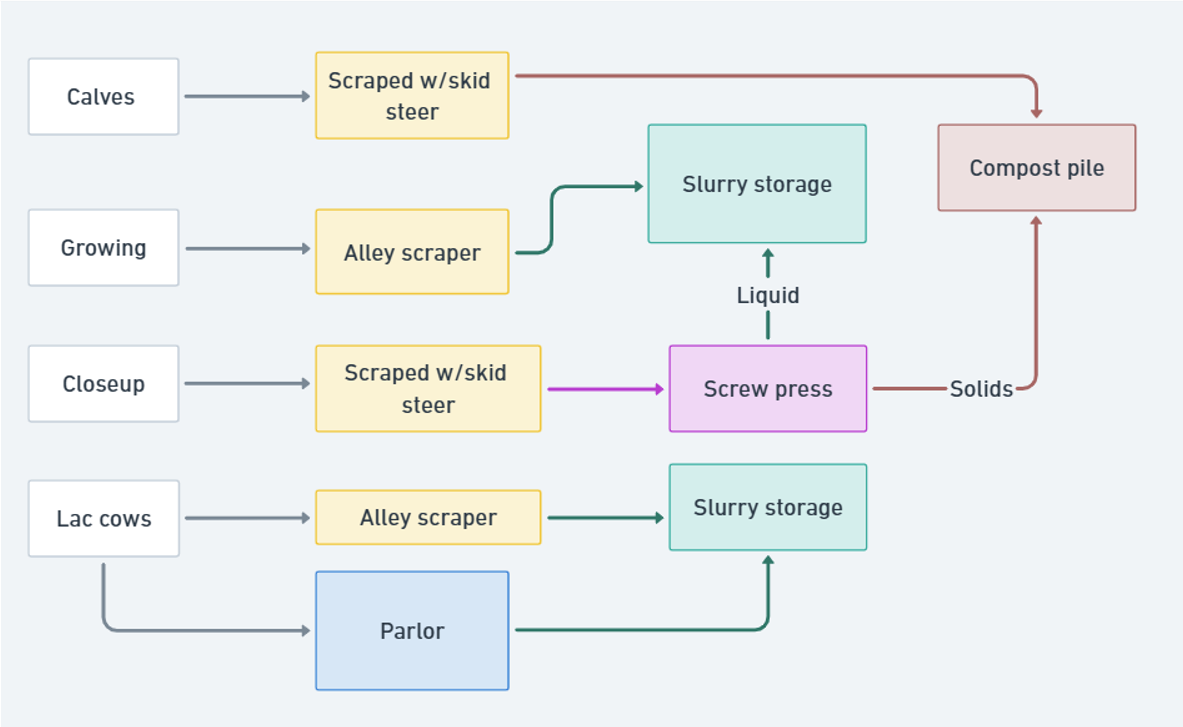
\includegraphics[width=0.9\textwidth]{resources/manuremanchain.png} % Replace with your image file
    \caption{A real-world example of a simplistic manure management chain.  }
       \end{figure}




    \begin{figure}[H] % The 'p' option places the figure on a page by itself
    \centering
    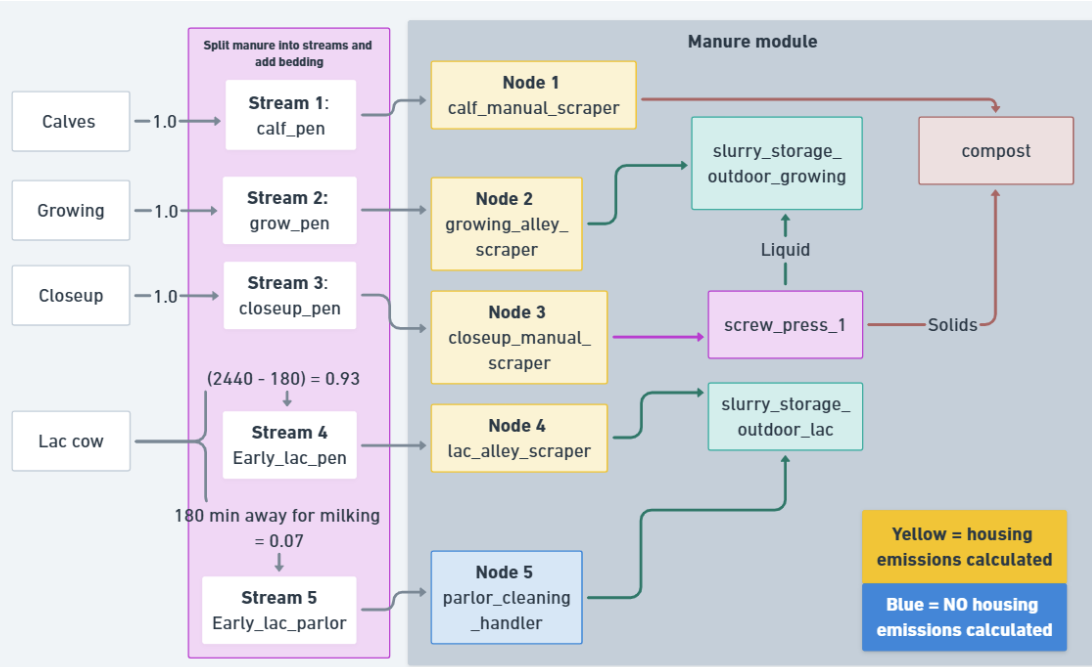
\includegraphics[width=0.9\textwidth]{resources/overviewmanure.png} % Replace with your image file
    \caption{The manure management chain illustrated in the previous figure, with RuFaS-specific information reflected. }

    \end{figure}


\subsection{Overview of Required Inputs}
There are two general categories of input required from the user: 
	\begin{enumerate}
            \item Which processors are used and how do they work (processor-specific configurations) E.g., storage time length, use of a cover 
            \item Destination and proportion(s) allocated to destination(s) of manure passed from each processor 
	\end{enumerate}


Information on inputs required and options available for each individual processor are outlined in the individual processor documentation. 
\vspace{0.2cm}

For defining destinations and proportions, there are very few rules and restrictions on how manure can be moved between processors. The primary rule for defining processor destinations is that users cannot define loops, i.e., manure from a processor “downstream” in a manure management chain cannot return its manure to a processor “upstream”.
\vspace{0.2cm}

\begin{tcolorbox}[colback=white, colframe=black, boxrule=0.5pt, arc=3pt, width=\textwidth]
The assignment of manure generated in the Animal Module (which also reflects the quantity of bedding used) to its destination in the Manure Module occurs in the Animal Module. See the Animal to Manure Connection section for more information. 

\end{tcolorbox}
\vspace{0.2cm}

\subsection{General Assumptions of the Manure Module}
        \begin{enumerate}
            \item All manure is recovered unless otherwise specifically stated. For example, all manure excreted by animals is assumed to be captured by manure handlers, all manure in a manure storage is assumed to be completely removed when the storage is emptied (unless explicitly noted in the specific processor’s documentation), etc. 
            \item Manure moves through the manure management chain once, and only once, per day. With this, values are reported on a daily timestep, and represent the current state at the end of the given day (e.g. CH\textsubscript{4} emissions from this day, amount of N left in storage on this day, etc.). 
                \begin {itemize}
                    \item Storage processors include a user-defined “storage time”, during which manure accumulates in the storage until reaching the end of the time interval, at which point it is passed to the next processor or exported, if the storage comes last in the manure chain.  The minimum storage time value is 1, thus manure cannot move through more than one storage per day. 
                    \item For processors without a storage time option, manure is assumed to move through the processor immediately. E.g., on a single day, excreted manure may move through a handler, continuous mix digester, separator, and into composting storage, with each processor reporting the quantity and composition of manure they either passed to the next processor or are holding in storage.
                \end{itemize}
            \item The Manure Module adheres to the principle of mass balance, meaning, the quantity of manure nutrients remaining in manure is proportional to the quantity of the nutrient lost through biological or physical processes. The same is true for additions of mass/nutrients.
                \begin{itemize}
                    \item One current exception to this is N loss. N losses are not currently reflected in the total mass of manure; this exception will be addressed and corrected in the near future. 
		      \end{itemize}
        \end{enumerate}

\textbf{Manure Storage Assumptions}
	\begin{enumerate}
            \item Received manure nutrients entering a storage are added to accumulated mass/nutrient quantities prior to calculating gas emissions each day.
            \item When the end of the storage’s user defined storage time is reached, the accumulated manure in storage is removed completely and entirely, and is passed to the next processor in the chain (e.g., a subsequent storage, field application, etc.).
            \item Emptying intervals (in days) are defined by the user in equal lengths at this time, e.g., manure storage can be emptied every 3 months (e.g. in April, July, October, January) but cannot be emptied in April, then 2 months later in June, and then 3 months later in September. However, timing of storage emptying (e.g. April and October emptying vs. May and November emptying) can be set according to the general simulation dates to simulate more realistic manure removal behavior.
	\end {enumerate}


\section{Animal and Manure Module Connection} 
\subsection{Introduction}

    Though animals are typically fed and managed in groups, referred to as pens in RuFaS, manure from a single group of animals may not always remain in or be transported to the same location on the farm. For example, lactating cows who must travel to a milking parlor deposit some proportion of their manure outside of their pen. Or, in open lot systems, manure deposited in the concrete feed alley apron is often removed and managed separately from manure deposited on the lot surface. Additionally, more than one type of bedding may be used in a pen (e.g., no bedding during summer but straw provided in winter), which also eventually becomes part of manure. Considering this, RuFaS accommodates routing of manure from a single group (pen) of animals to multiple locations, which are then received by the Manure module. This document describes how a pen’s total manure excretion and bedding are allocated to one or more discrete quantities of manure, referred to as manure streams, and passed to the Manure module. How the user configures this manure routing and bedding options and addition of bedding to manure are also described here.

    \vspace{0.25cm}
    \textbf{Implementation in RuFaS} 
    \vspace{0.25cm}

    The Animal module is responsible for calculating manure excretion mass and composition based on animal attributes, ration composition and intake, and other factors. The Animal module must then pass this manure on to the Manure module, where manure nutrient gains and losses are quantified through field application or export. The Animal module currently calculates manure excretion at the pen level (i.e., values representative of the total manure from animals in a single pen), and several additional steps must occur before manure information can be sent to the Manure module. These steps include:
    \vspace{0.2cm}

    \begin{itemize}
        \item Splitting manure from individual pens into one or more user-defined manure streams
        \item Repackaging manure information into the form and units utilized by the Manure module
        \item Applying bedding mass or nutrients to manure streams 
    \end{itemize}
    \vspace{0.2cm}
    
    The direct connection between Animal module, which captures the animal lifecycle, nutrient intake and excretion, and other factors, and the Manure module is a crucial part of the nutrient cycle in RuFaS.

    This document describes how the user defines the partitioning of manure from a single pen of animals into one or more manure streams, and the basic mathematical procedure for generating manure streams from excreted manure. Later it will review the options for and application of bedding to manure streams.
\vspace{0.3cm}

\textbf{Classes}
\vspace{ 0.3cm}
    
    \begin{table}[h!]
    \centering
    \renewcommand{\arraystretch}{1.3}
    \caption{List of Python classes for Animal to Manure Module connection.}
    \begin{tabular}{@{} L{3cm} L{9cm}  @{}}
    \toprule

    \multicolumn{1}{c}{\textbf{Handlers}} & 
    \multicolumn{1}{c}{\textbf{Description}} \\
    \midrule
    Pen  & pen.py; Translates pen-level manure information into the format and units required by the Manure module; Translates pen-level manure information into one or more ManureStream instance(s), if applicable, and creates accompanying PenManureData instances  \\
    PenManureData & animal\_to\_manure\_connection.py; Generates PenManureData and ManureStream \\

    \bottomrule
    \end{tabular}
    \end{table}  

\textbf{Required User Inputs }

\renewcommand{\arraystretch}{1.3}
\begin{longtable}{@{} L{3cm} L{3cm} L{1.5cm} L{8cm} @{}}
\caption{User inputs for Stream Formation and Bedding sections.} \\
\toprule
\textbf{ } & 
\multicolumn{1}{c}{\textbf{Variable}} & 
\multicolumn{1}{c}{\textbf{Units}} & 
\multicolumn{1}{c}{\textbf{Description}} \\
\midrule
\endfirsthead

\multicolumn{4}{@{}l}{\textit{Table continued from previous page}} \\
\toprule
\textbf{ } & 
\multicolumn{1}{c}{\textbf{Variable}} & 
\multicolumn{1}{c}{\textbf{Units}} & 
\multicolumn{1}{c}{\textbf{Description}} \\
\midrule
\endhead

\midrule
\multicolumn{4}{r}{\textit{Continued on next page}} \\
\endfoot

\bottomrule
\endlastfoot

\multirow{7}{*}{\textbf{Stream Formation}} 
& minutes\_away\_for \_milking & minutes & The total time (minutes) per day that animals spend walking to/from the parlor, waiting in holding areas, or being actively milked. For non-lactating animals, this value may be omitted or entered as “null”. \\ 
& first\_parlor\_processor & – & The name of the processor defined in the Manure module inputs that manure from the milking parlor should enter. \\ 
& parlor\_stream\_name & – & The user-defined name of this pen’s parlor stream. \\ 
& stream\_name & – & The user-defined name of this stream. \\ 
& bedding\_name & – & The name of the specific bedding configuration used with this stream. See section 2 for more information. \\ 
& stream\_proportion & 0–1 & The proportion of daily manure excreted outside of the parlor and while traveling to/from the parlor that enters this stream. All stream proportions within a pen must sum to 1.0. Optional if only one stream. \\ 
& first\_processor & – & The name of the processor defined in the Manure module inputs that this ManureStream should enter. \\ 

\cmidrule(lr){1-4}

\multirow{9}{*}{\textbf{Bedding}} 
& name & – & Unique identifier to reference this bedding configuration. \\ 
& bedding\_type & – & The type of bedding material. Options: sand, straw, sawdust, manure solids, or none. \\ 
& bedding\_mass \_per\_day & kg/day & Daily mass of fresh bedding added per animal per day (wet weight). Bedding mass is applied based on the total number of animals in the pen, and is not based on the stream proportion of the manure stream the bedding is assigned to. \\ 
& bedding\_density & kg/m\textsuperscript{3} & Density of the bedding on a wet weight basis. \\ 
& bedding\_dry\_matter \_content & fraction & Bedding dry matter content as a fraction of total mass. \\ 
& bedding\_carbon \_fraction & fraction & Bedding carbon content as a fraction of total mass. \\ 
& bedding\_phosphorus \_content & fraction & Bedding phosphorus content as a fraction of total mass. \\ 
& sand\_removal \_efficiency & fraction & Fraction of sand assumed to be removed immediately after manure removal. \\

\end{longtable}


\textbf{Other inputs}\\

\begin{itemize}
\item Instances of PenManure objects that represent manure excreted by single pens of animals in the Animal module. See Animal Excretions documentation for further details. 
\item Instances of Pen objects that represent pen information for single pens of animals in the Animal module.
\end{itemize}

\vspace{0.3cm}

\textbf{Expected Outputs}
\vspace{ 0.25cm}

\textbf{\textit{Stream Formation}}
\begin{itemize}
    \item Instance(s) of a ManureStream for each manure stream defined by the user that represent the attributes of the manure in the specific manure stream. ManureStream instances include the following variables (all in kg except for volume, \(m^3\) and manure methane potential, \(m^3 / kgVS\)):
    \begin{itemize}
        \item water 
        \item ammoniacal\_nitrogen
        \item nitrogen 
        \item phosphorus
        \item potassium
        \item ash
        \item manure\_degradable\_volatile\_solids
        \item manure\_non\_degradable\_volatile\_solids
        \item bedding\_non\_degradable\_volatile\_solids
        \item total\_solids
        \item mass (equal to sum of water and total solids)
        \item total volatile solids (equal to sum of degradable and non-degradable volatile solids)
        \item volume
        \item methane\_production\_potential

    \end{itemize}

    \item A PenManureData class instance for each manure stream defined by the user, that represents the attributes of the animals and pen from which the manure originated. PenManureData instances include the following variables, reported by the Animal module:
    \begin{itemize}
        \item num\_animals: number of animals present in the pen from which the manure stream originated. Note that this variable does not correspond to the number of animals that generated the manure contained in the stream.
        \item manure\_deposition\_surface\_area: the surface area soiled with manure, used in the determination of housing emissions. See the Manure Handler document for information on determination of this value (MN.HDL.4). 
        \item animal\_combination: the type of animal contained in the pen (calf, growing, closeup, or lactating).
        \item pen\_type: the type of pen (freestall, tiestall, open lot, or bedded pack barn) the manure in this stream originated from. 
        \item manure\_urine\_mass (kg): mass of urine in the manure.
        \item manure\_urine\_nitrogen (kg): mass of urine N in the manure.
        \item steam\_type: the type of ManureStream (parlor stream or general stream).
        \item first\_processor: the name of the processor defined in the Manure module inputs that this ManureStream should enter. 
        \item total\_bedding\_mass (kg): the total mass of bedding added to this stream. 
        \item total\_bedding\_volume ( m\textsuperscript{3}): the total volume of bedding added to this stream.
    \end{itemize}
\end{itemize}
\textbf{\textit{Bedding}}
\begin{itemize}
    \item total\_bedding\_mass: The total mass of bedding added to the ManureStream each day (kg).
    \item total\_bedding\_volume: The total mass of bedding added to the ManureStream each day (kg).
\end{itemize}



\vspace{0.2cm}





\subsection{Methodology}
\textbf{\textit{Stream Formation}}
\vspace{0.25cm}

How many discrete locations/quantities (i.e., manure streams) a single pen’s manure is split into is determined by the user. There are two types of manure streams in the model: 
\vspace{0.5cm}

Parlor: A stream representing manure deposited in or while traveling to/from the milking parlor, along with (fresh, non-recycled) wash water. 
    \begin{itemize}
        \item A parlor stream is not directly defined by the user for each pen in the way general streams are; parlor streams are created automatically for each lactating pen. The user specifies the proportion of each lactating pen’s total manure that enters the parlor stream via the minutes away for milking input. Time away from the pen for milking can vary greatly between farms but also is typically known by the farm management, as fetching and pushing cows to the parlor is an intentional daily activity. This makes time away from the pen for milking (minutes\_away\_for\_milking) a simple and relatively reliable metric for determining the basic split of manure in the housing area vs. milking parlor. 
        \item Only one parlor stream can be created per lactating cow pen. However, more than one milking parlor (destination for milking parlor manure) may be defined for a farm; the user simply assigns parlor streams to differing instances of a parlor cleaning handler, which represents the milking parlor. See Manure Handler documentation for more information. 
        \item No bedding can be applied to parlor streams.
    \end{itemize}

General: A stream representing all or a portion of non-parlor manure and bedding. Manure in this stream or streams represents manure excreted outside the milking parlor or traveling to/from the parlor. 
    \begin{itemize}
        \item All pens must have at least one general stream defined. 
        \item Theoretically, an infinite number of general streams can be defined per pen, as long as stream proportions are provided for all of them. However, most practical farm simulation scenarios will require only one or two general manure streams per pen.
        \item The number of general streams and the proportion of non-parlor manure entering each stream is directly defined by the user. Stream proportion logic is covered below.
    \end{itemize}

General-type manure streams are defined in the animal inputs, within each Pen blob. Each pen includes a “manure\_streams” array input in which the user defines the one or more general manure streams generated by this specific pen. The required inputs and their definitions are described above in the Inputs section; these inputs must be provided for each manure stream as outlined in the figure below.


    \begin{figure}[H] % The 'p' option places the figure on a page by itself
    \centering
    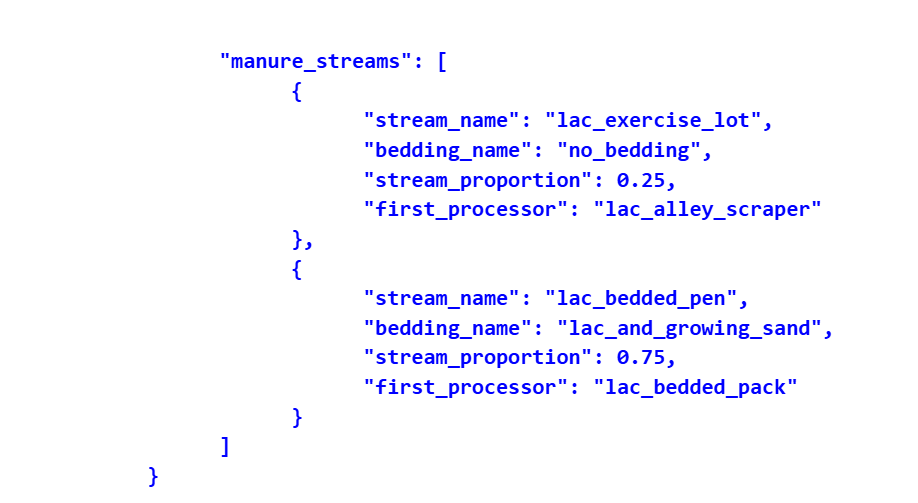
\includegraphics[width=0.9\textwidth]{resources/manurestreams.png} % Replace with your image file
    \caption{If manure from a pen is routed to two different general manure streams, two sets of manure stream inputs must be defined. An example of a single pen’s manure stream inputs is above - in this example, manure from this pen is routed to two locations, one representing an exercise lot, the other representing a bedded pack area.}

    \end{figure}


\textbf{Stream proportion logic}
\vspace{ 0.25cm}

The stream proportion refers to the user-defined proportion (0 to 1) of manure generated by animals in a single pen that enters a specific manure stream. The translation of user-defined stream proportions into the effective stream proportion utilized by the model is described below. This effective proportion is referred to as the split ratio in the model code - it is the value by which total manure excretions are multiplied by to determine the quantity of any single nutrient allocated to a stream of any type (e.g., 20\% (0.20) to parlor stream, 40\% (0.40) to general stream 1, 40\% (0.40) to general stream 2. The values are the split ratios). 

\textbf{Non-lactating pens} If more than one general stream is defined for a single pen, a stream proportion must be provided for each stream, and manure will be allocated to streams according to these proportions. Essentially, the split ratio is equal to the user-defined stream proportion.


\textbf{Lactating pens} 

\textit{Parlor streams}: The user-defined minutes away for milking is used to calculate the stream proportion value for the milking parlor:
\vspace{0.2cm}

\textbf{When:}
    \begin{center}
        \(parlor\_stream\_proportion = \frac{minutes\_away\_for\_milking }{ 1440}\)
    \end{center}
        \vspace{0.5cm}
    
            {\raggedleft \textbf{[AN.PEN.1]}\par}
            \vspace{0.5cm}

    \begin{itemize}
        \item minutes\_away\_for\_milking: user-defined total minutes per day lactating cows spend out of the pen traveling to/from the parlor or being milked.
        \item 1440: minutes per day.

    \end{itemize}

\textit{General streams} Each general stream proportion represents the fraction of manure—excluding that deposited in or during travel to/from the milking parlor—that enters a specific manure stream. For example, if all manure outside the parlor enters one stream, its proportion would be 1.0. If manure outside the parlor was split evenly between two general streams, each stream’s proportion would be 0.50. With this, the effective proportion of total manure entering this stream (the split ratio) must be calculated according to the parlor stream proportion.


First, we determine the proportion of manure entering any and all general streams vs. the parlor stream.
\vspace{0.2cm}

    \begin{center}
        \(total\_general\_stream\_portion = 1 - parlor\_stream\_proportion\)
    \end{center}
        \vspace{0.5cm}
    
            {\raggedleft \textbf{[AN.PEN.2]}\par}
            \vspace{0.5cm}
            
\textbf{When:}
    \begin{itemize}
        \item parlor\_stream\_proportion: proportion of total manure allocated to the parlor stream, calculated in \textbf{[AN.PEN.1]}.
    \end{itemize}

Once we have derived the proportion of manure entering any/all general streams, we multiply this proportion by the user-defined general stream proportion(s), to determine the split ratio for each general stream.
\vspace{0.2cm}

    \begin{center}
        \(general\_stream\_proportion = total\_general\_stream\_proportion * stream\_proportion\)
    \end{center}
        \vspace{0.5cm}
    
            {\raggedleft \textbf{[AN.PEN.3]}\par}
            \vspace{0.5cm}

To continue with our example from above, if cows spent 200 minutes per day in the milking parlor, their split ratios would be as follows: 
\vspace{0.25cm}

\textbf{Parlor:}
\vspace{0.2cm}

\( \frac{200}{1440} = 0.140\)
\vspace{0.1cm}

\(lac\_exercise\_lot: (1 - 0.139) * 0.25 = 0.215\)
\vspace{0.1cm}

\(lac\_bedded\_pen: (1 - 0.139) * 0.75 = 0.645\)
\vspace{0.3cm}

\textbf{Recommended defaults}
\vspace{0.2cm}

Although the time away from a pen is highly variable and specific to each farm’s infrastructure and management, some recommended defaults for situations where actual information is not available are provided below. 
\vspace{0.15cm}

\textit{Minutes away for milking}
\vspace{0.1cm}

Recommended minutes\_away\_for\_milking values for lactating cows are based on cow time budgets from published literature and are not official model defaults. The purpose of these time budgets at the time of writing is strictly related to estimating manure deposition in specific locations and is not related to larger Animal module activities. The use of time budgets for this purpose relies on the assumption that cows excrete urine and feces at a constant rate throughout the day and across various locations.
\vspace{0.1cm}


\clearpage
\begin{sidewaystable}
     \caption{Recommended minutes\_away\_for\_milking by pen type based on published literature. Remember, this does not necessarily reflect the model defaults. }
\centering
\renewcommand{\arraystretch}{1.3}


\begin{tabular}{@{} L{2cm} L{4cm} L{1.5cm} L{8cm} @{}}
\toprule

\multicolumn{1}{c}{\textbf{Pen Type}} & 
\multicolumn{1}{c}{\textbf{minutes\_away\_for\_milking}}  & 
\multicolumn{1}{c}{\textbf{Proportion}}  & 
\multicolumn{1}{c}{\textbf{Special Notes}} \\
\midrule


Freestall\textsuperscript{1} & 200 m (3.33 h) & 0.139 &     \\
Tiestall & 200 m (3.33 h) & 0.139 & Limited data; value is based on the assumption that daily time away from pen for milking will be broadly similar between freestall and tiestall barns.\textsuperscript{2} \\
Open lot & 300 m (5 h) & 0.208 & Assumption that open lot pens tend to be considerably larger than indoor-housed systems (greater travel distance).\textsuperscript{3}
 \\
Compost bedded pack barn & 200 m (3.33 h) & 0.139 & Limited data; value is based on the assumption that daily time away from pen for milking will be broadly similar between freestall and tiestall barns.\textsuperscript{2} \\
\bottomrule
\multicolumn{4}{l}{\footnotesize \textsuperscript{1} \cite{gomez2010time}, \cite{espejo2007herd}} \\
\multicolumn{4}{l}{\footnotesize \textsuperscript{2} \cite{jewell2019prevalence}} \\
\multicolumn{4}{l}{\footnotesize \textsuperscript{3} \cite{meyer2019contract}} \\

\end{tabular}

\end{sidewaystable}





\textit{Open lot and bedded pack systems}
\vspace{0.1cm}

The management of open lot and bedded pack barn pens often results in manure from a single pen being managed in multiple ways. These types of pens often have designated resting areas (i.e. the harrowed lot or bedded pack) where manure is managed in place for an extended period, as well as a separate feeding area, such as a concrete apron along a feed alley. Manure deposited in this area may be scraped back into the resting area, or it may be flushed, vacuumed or scraped to another separate storage area. Two distinct manure management routines within a single pen indicate that two manure streams should likely be used. If this is the case, the user may reference the tables below as a starting point for defining stream proportions representing the resting vs. feeding area. Defining two separate manure streams is recommended where appropriate to ensure that manure is not over-allocated to the parlor manure stream (where it does not contribute to housing emission estimations) and bedding is allocated appropriately. 


The following streams and proportions are based on literature data and are not official model defaults. They are provided for user informational purposes; they may be used as a starting point to adjust proportions specific to a farm, or can be used for theoretical modeling scenarios. 
\vspace{ 0.25cm}


\begin{table}[h!]
\centering
\renewcommand{\arraystretch}{1.3}
\begin{center}
    \caption{Proportions of differnt streams for different animal classes.}
\end{center}
\vspace{-0.5cm}

\begin{tabular}{@{} L{5cm} L{4cm} L{1.2cm} L{1cm} L{0.8cm} L{0.75cm} @{}}
\toprule
\multicolumn{1}{c}{\textbf{Pen Type}} & 
\multicolumn{1}{c}{\textbf{Animal Class}}  & 
\multicolumn{1}{c}{\textbf{Lactating}}  & 
\multicolumn{1}{c}{\textbf{Closeup}}  & 
\multicolumn{1}{c}{\textbf{Growing}}  & 
\multicolumn{1}{c}{\textbf{Calves}} \\


\midrule

\multirow{3}{*}{\textbf{Open lot or bedded pack barn} \textsuperscript{1}} 
& General stream, lot        & 0.796 & 0.76  & 0.76  & 1    \\
& General stream, feed alley & 0.204 & 0.24  & 0.24  & N/A  \\
& minutes\_away\_for\_milking & 300   & N/A   & N/A   & N/A  \\
\cmidrule(lr){1-6}
\multirow{3}{*}{\textbf{Bedded pack barn} \textsuperscript{2}} 
& General stream, bedded pack & 0.792 & 0.819 & 0.819 & 1    \\
& General stream, feed alley  & 0.208 & 0.179 & 0.179 & N/A  \\
& minutes\_away\_for\_milking & 200   & N/A   & N/A   & N/A  \\

\bottomrule
\multicolumn{6}{p{\linewidth}}{\footnotesize\raggedright 
\textsuperscript{1} Based on data from \cite{meyer2019contract} and the assumption that open lot pens tend to be considerably larger than indoor-housed systems (greater travel distance). \par
\textsuperscript{2} Based on data from \cite{endres2007behavior}, which suggests behavior of cows in compost bedded pack barns is broadly similar to those in other housing systems. With this, freestall data from \cite{gomez2010time} was used, which reported 4.3 hours of feeding time, 3.33 hours away for milking, and the remainder spent in the housing area.
} \\


\end{tabular}
\end{table}




\textit{Passing information to the Manure module}
\vspace{0.1cm}

Once split ratios have been determined for each manure stream in each pen, Animal module manure and pen data can be translated into ManureStream objects. The variables contained in ManureStream are below; this dataclass is used both to move information from Animal to Manure module, as well as move information between processors within the Manure module. 


The majority of the variables are calculated in the Animal module and translated directly into a ManureStream object. Subbullets below a variable indicate how variables not directly reported by the Animal module are calculated. 
\vspace{0.2cm}

\textbf{\textit{Bedding}}
\vspace{0.25cm}

Bedding is assigned and applied by manure stream, not by pen. The following calculations described how bedding mass, nutrients, and volume are calculated, and how bedding is added to a manure stream.\\

\textbf{Calculate total bedding mass}
\vspace{ 0.25cm}

calc\_total\_bedding\_mass

\vspace{0.2cm}

    \begin{center}
        \(total\_bedding\_mass (kg) = bedding\_mass\_per\_day (kg/animal) * num\_animals * sand\_removal\_efficiency \)
    \end{center}
        \vspace{0.5cm}
    
            {\raggedleft \textbf{[AN.PEN.7]}\par}
            \vspace{0.5cm}

\textbf{When:}
    \begin{itemize}
        \item bedding\_mass\_per\_day: The user-inputted bedding mass applied per animal per day. Note that this input is per total number of animals housed in the pen.
        \item num\_animals: Animals in the pen from which the manure stream originated.
        \item sand\_removal\_efficiency: User-defined proportion of sand bedding removed via sand settling lane or other sand recovery technology. This value is only utilized if bedding type \= sand.
    \end{itemize}

\textbf{Calculate total bedding volume}
\vspace{ 0.25cm}

calc\_total\_bedding\_volume

\vspace{0.2cm}

    \begin{center}
        \(total\_bedding\_volume (m^3) = \frac{total\_bedding\_mass (kg)}{bedding\_density (kg/m^3)}  \)
    \end{center}
        \vspace{0.5cm}
    
            {\raggedleft \textbf{[AN.PEN.8]}\par}
            \vspace{0.5cm}

\textbf{When:}
    \begin{itemize}
        \item total\_bedding\_mass (kg): the total mass of bedding applied to the manure stream each day, calculated in \textbf{[MN.PEN.7]}.
        \item bedding\_density (kg/m\textsuperscript{3}): user-defined density of the specified bedding.

    \end{itemize}

\textbf{Calculate total bedding dry solids}
\vspace{ 0.25cm}

calc\_total\_bedding\_dry\_solids

\vspace{0.2cm}

    \begin{center}
        \(total\_bedding\_dry\_solids (kg) = total\_bedding\_mass (kg) * bedding\_dry\_matter\_content  \)
    \end{center}
        \vspace{0.5cm}
    
            {\raggedleft \textbf{[AN.PEN.9]}\par}
            \vspace{0.5cm}

\textbf{When:}
    \begin{itemize}
        \item total\_bedding\_mass (kg): the total mass of bedding applied to the manure stream each day, calculated in \textbf{[MN.PEN.7]}.
        \item bedding\_dry\_matter\_content: user-defined dry matter content of the specified bedding.

    \end{itemize}

\textbf{Calculate total bedding water}
\vspace{ 0.25cm}

calc\_total\_bedding\_water

\vspace{0.2cm}

    \begin{center}
        \(total\_bedding\_water (kg) = total\_bedding\_mass (kg) * (1 - bedding\_dry\_matter\_content) \)
    \end{center}
        \vspace{0.5cm}
    
            {\raggedleft \textbf{[AN.PEN.10]}\par}

\textbf{When:}
    \begin{itemize}
        \item total\_bedding\_mass (kg): the total mass of bedding applied to the manure stream each day, calculated in \textbf{[MN.PEN.7]}.
        \item bedding\_dry\_matter\_content: user-defined dry matter content of the specified bedding.

    \end{itemize}
    \vspace{0.5cm}

\textbf{Update ManureStream values to reflect bedding}
\vspace{0.15cm}

\_apply\_bedding (pen.py)
\vspace{0.2cm}

\begin{table}[h!]
\centering
\renewcommand{\arraystretch}{1.3}
\begin{center}
    \caption{Calculated manure and bedding characteristics}
\end{center}
\vspace{-0.2cm}

\begin{tabular}{@{} L{3cm} L{2cm} L{9cm} @{}}
\toprule
\multicolumn{1}{c}{\textbf{Variable}} & 
\multicolumn{1}{c}{\textbf{Units}} & 
\multicolumn{1}{c}{\textbf{Calculation}} \\
\midrule

water  & kg & ManureStream water (kg) + bedding\_water (kg) \\
ash  & kg & if bedding type = sand, ash (kg) = total\_bedding\_mass (kg); otherwise, ash = 0 \\
phosphorus  & kg & ManureStream phosphorus + total\_bedding\_mass (kg) * bedding\_phosphorus\_content) \\
non\_degradable \_volatile\_solids & kg & If bedding type = sand, ManureStream non\_degradable\_volatile\_solids (kg); If bedding type is not sand, ManureStream non\_degradable\_volatile\_solids (kg) + total\_bedding\_dry\_solids (kg) \\
total\_solids  & kg & ManureStream total\_solids (kg) + total\_bedding\_dry\_solids (kg) \\
volume  &  m\textsuperscript{3} & ManureStream volume ( m\textsuperscript{3}) + total\_bedding\_volume ( m\textsuperscript{3}) \\


\bottomrule
\end{tabular}
\end{table}



\section{Manure Handler}
\subsection{Introduction}
    \vspace{0.2cm}
    
    Manure handling refers to the method of managing manure in animal living spaces. For some housing/pen types, such as freestalls and tiestalls, this involves removing the manure from barn alleyways, and is usually accomplished using some form of scraping or flushing with water. Flush systems utilize water to remove the manure from alleyways, whereas scrape systems use little or no water. For other housing types like open lots and compost bedded pack barns, tillage or harrowing are commonly used to instead incorporate the manure, urine, bedding (if applicable) and air into the pack and allow it to dry. 
    \vspace{0.5cm}

    The specific manure handler options in the RuFaS model are:
    \begin{itemize}
        \item \textbf{Flushing} 
        \vspace{0.15cm}

        Flushing involves using water to carry manure and soiled bedding away from housing areas. A series of pipes and channels direct water to wash the manure into a collection pit. Flushing helps maintain a cleaner environment for animals and reduces the buildup of manure on the floor. Flushing/recirculating may also be used to “lubricate” transport/pumping of manure from under-floor collection pits to the next manure management step. Flushing is commonly performed using recycled water from a solid liquid separator, liquid manure storage, or other liquid collection area, rather than using fresh water.

        \item \textbf{Manual Scraping} 
        \vspace{0.15cm}

        Scraping involves physically removing the manure and soiled bedding using equipment like tractor-mounted scrapers or skid steers, or the manual use of shovels/scrapers, etc. This method is typically used in barns with slatted or solid floors. Regular scraping prevents manure accumulation and provides a clean area for animals.

        \item \textbf{Alley Scraper} 
        \vspace{0.15cm}

        A scraper blade, typically pulled along by a chain or cable, moves slowly down a pen or alleyway on a set schedule several times a day, pushing or pulling manure out of the pen/alley. The function and outcome is similar to manual scraping, but alley scrapers are mechanized and typically operate automatically.

        \item \textbf{Parlor Cleaning} 
        \vspace{0.15cm}

        Parlor cleaning is a RuFaS-specific handler that represents cleaning of manure from milking units, parlor stall floors, and other areas in the milking parlor that require the use of fresh, non-recycled water. Parlor cleaning also can include an optional flush system capability, which functions in the same manner as the flush system described above and is used to wash manure from holding area floors.
        
    \end{itemize}




Manure handlers in RuFaS have two primary functions: calculate and add cleaning water if used, and calculate indoor housing emissions of CH\textsubscript{4}, CO\textsubscript{2}, and NH\textsubscript{3} if applicable.
\vspace{0.2cm}

    The following are important assumptions made in the manure handler submodules, as well as context on how manure handlers are used in the larger manure management chain:
    \begin{enumerate}
        \item All manure excreted and all bedding applied each day (if applicable) is assumed to be recovered by the manure handler. 
        \item Manure handlers in RuFaS are intended to be utilized, at this time, with manure deposited in housing areas that is cleaned frequently (e.g., removed daily or every few days), such as indoor barn floors, or concrete feed alleys in open lot or compost bedded pack pens. Handlers should not be used in manure streams where manure resides for a long period of time, such as streams representing an open lot or bedded pack manure pack, that have a designated processor (i.e., Open Lot or Bedded Pack). Users can consider the manure handler functionality to be “built in” to these processors. Defining a handler prior to one of these types of processors will result in double-counting of housing emissions. 
        \item If a manure handler is used, it must be defined first in the manure management chain. This prevents inappropriate calculation of housing emissions “downstream” when manure is no longer in the animal housing area. Handlers are meant to represent manure handling in animal living spaces; other manure handling/transport systems such as pumps, augers, belts, etc. are not explicitly modeled in RuFaS. 
    \end{enumerate}

\newpage
\textbf{Classes}
\vspace{ 0.25cm}

    \begin{table}[h!]
    \begin{center}
        \caption{The classes of handlers that are used in this module.}
    \end{center}
\vspace{ -0.5cm}

    \centering
    \renewcommand{\arraystretch}{1.3}

    \begin{tabular}{@{} L{5cm} L{7cm}  @{}}
    \toprule

    \multicolumn{1}{c}{\textbf{Handlers}} & 
    \multicolumn{1}{c}{\textbf{Description}} \\
    \midrule
    Handler (Processor)  & handler.py contanins basic methods that are applicable to all handlers  \\
    Single StreamHandler (Handler)  & single\_stream\_handler.py contains alley screaper, manual scraping, and flush system-specific methods \\
    ParlorCleaning (Handler)  & parlor\_cleaning.py contains parlor cleaning-specific methods  \\
    \bottomrule
    \end{tabular}
    \end{table}  

\textbf{Required User Inputs }
\vspace{0.25cm}



    \begin{table}[h!]
    \centering
    \renewcommand{\arraystretch}{1.3}
    \begin{center}
        \caption{Required inputs for the Manure Handler (refreshed\_manure\_management.json)}
    \end{center}
    \vspace{-0.2cm}

    \begin{tabular}{@{} L{4.5cm} L{2cm} L{8cm} @{}}
    \toprule
    \multicolumn{1}{c}{\textbf{Variable}} & 
    \multicolumn{1}{c}{\textbf{Units}} & 
    \multicolumn{1}{c}{\textbf{Description}} \\
    \midrule
Name & none &  Unique identifier of the specific handler configuration used. \\ 
Type & none &  The type (alley scraper, manual scraping, flushing, or parlor scraping) of manure handler. \\ 
cleaning\_water\_use\_amount  & L/animal/day &  The rate of water use (L per animal per day, total of fresh and/or recycled water) by a specified manure handler. \\ 
cleaning\_water\_recycle\_fraction & none &  The fraction (0.XX) of cleaning water used by a specified handler that is from recycled (not fresh) water sources. \\ 
use\_parlor\_flush  & true/false &  True/false indication for if a parlor flush (which may be partially or fully recycled water) is used in addition to routine parlor water cleaning with fresh water. \\ 

    \bottomrule
    \end{tabular}
    \end{table}  
    \vspace{ 0.25cm}
    
\textbf{Other inputs}\\
Instance(s) of ManureStream for each manure stream defined by the user that represent the attributes of the manure in the specific manure stream. ManureStream instances include the following variables (all in kg except for volume, \(m^3\) and manure methane potential, \(m^3 / kgVS\)):
    \begin{itemize}
        \item water 
        \item ammoniacal\_nitrogen
        \item nitrogen 
        \item phosphorus
        \item potassium
        \item ash
        \item manure\_degradable\_volatile\_solids
        \item manure\_non\_degradable\_volatile\_solids
        \item bedding\_non\_degradable\_volatile\_solids
        \item total\_solids
        \item mass (equal to sum of water and total solids)
        \item total volatile solids (equal to sum of degradable and non-degradable volatile solids)
        \item volume
        \item methane\_production\_potential

    \end{itemize}

Manure handlers also make use of information contained in the PenManureData subclass. This includes the following information specific to the pen from which the manure was generated:
\begin{itemize}
    \item num\_animals: number of animals in the pen
    \item animal\_combination: type of animals in the pen (calves, growing post-weaning heifers through closeup period), closeup (cows and heifers within user-defined closeup period), or lactating cows)
    \item Manure deposition surface area (m2): surface area soiled with manure. See section below on determining soiled surface area
    \item pen\_type: the type of pen the manure was generated in (freestall, tiestall, open lot, or bedded pack barn)
    \item daily\_urine (kg): mass of urine in the manure
    \item urine\_nitrogen (kg): mass of urine N in the manure
    \item stream\_type: the type of manure stream the manure is in (parlor or general stream)

\end{itemize}
\begin{tcolorbox}[colback=white, colframe=black, boxrule=0.5pt, arc=3pt, width=\textwidth]
Note that stream\_type is not a user input, it is automatically assigned. Parlor streams are created automatically and all other streams are assigned “general”.
\end{tcolorbox}


\textbf{Expected Outputs}
\vspace{ 0.25cm}
\begin{itemize}
    \item All handler types:
    \begin{itemize}
        \item ManureStream variables
        \item total\_cleaning\_water\_volume ( m\textsuperscript{3}): total volume of fresh (non-recycled) cleaning water used for, and ultimately added to, a single manure stream on a single simulation day by the manure handler
        \item barn\_temperature (\(\circ C\)): ambient temperature in barn
    \end{itemize}
    \item Alley scraper, manual scraping, flush system:
    \begin{itemize}
        \item housing\_methane (kg): daily CH\textsubscript{4} (kg) emitted from manure on barn floors
        \item housing\_ammonia\_N\_emissions: (kg): daily NH\textsubscript{3}-N (kg) emitted from manure on barn floors
        \item housing\_carbon\_dioxide (kg): daily CO\textsubscript{2} (kg) emitted from manure on barn floors
    \end{itemize}

\end{itemize}


\subsection{Methodology}


\textbf{Calculate barn temperature}
\vspace{ 0.25cm}

\_determine\_barn\_temperature

Air temperature inside barns is, in general, slightly cooler than the outdoors during the day, and slightly-to-considerably warmer than the outdoor temperature overnight, depending on the season. With this, basic bounds were implemented in the determination of barn temperature. These bounds were suggested by manure SMEs and are supported by barn temperature ranges reported in \cite{Bucklin2009} (Florida, upper limit). The lower bound (5$^\circ$C) suggested by SMEs was based on general industry standards/conditions.

\vspace{ 0.25cm}
If ambient (outdoor) air temperature \(<\) 5$^\circ$C, barn temperature = 5$^\circ$C\\
If ambient (outdoor) air temperature \(>\) 5$^\circ$ \& \(<\) 30$^\circ$C, barn temperature = air temperature\\
If ambient (outdoor) air temperature \(>\) 30$^\circ$C, barn temperature = 30$^\circ$C\\


\textbf{Calculate cleaning/flushing fresh water addition}
\vspace{ 0.25cm}

determine\_handler\_cleaning\_water\_volume

The following method calculates the volume of fresh (non-recycled) cleaning water used for, and ultimately added to, a single manure stream on a single simulation day by the manure handler. This method is used in all handler types; however, for parlor cleaning handlers, this method is only utilized if “use\_parlor\_flush” is entered as true. If no water is used with the handler (user inputted cleaning water use rate = 0), the function will return 0.
\vspace{0.2cm}

    \begin{center}
        \(cleaning\_water \ (L) = num\_animals * (cleaning\_water\_use\_rate * (1 - cleaning\_water\_recycle\_fraction)) \)
    \end{center}
        \vspace{0.5cm}
    
            {\raggedleft \textbf{[MN.HDL.1]}\par}
            \vspace{0.5cm}

\textbf{When:}
    \begin{itemize}
        \item num\_animals: the number of animals in the pen assigned to the handler
        \item cleaning\_water\_use\_rate (L/animal/d): the user-provided cleaning water use rate for the handler
        \item cleaning\_water\_recycle\_fraction: the proportion of cleaning water that is from recycled, non-fresh sources

    \end{itemize}  
    \vspace{0.2cm}
    
Total fresh water added to manure (L) each day is calculated as follows: 
\vspace{0.2cm}

    \begin{center}
        \(total\_cleaning\_water (m^3) = (cleaning\_water (L) + fresh\_water\_volume\_used\_for\_milking (L)) * LITERS\_TO\_CUBIC\_METERS\)
    \end{center}
        \vspace{0.5cm}
    
            {\raggedleft \textbf{[MN.HDL.2]}\par}
            \vspace{0.25cm}
\textbf{When:}
    \begin{itemize}
        \item LITERS\_TO\_CUBIC\_METERS: a constant set to 0.997 kg/m\textsuperscript{3}

    \end{itemize}  

 
\textbf{Calculate milking parlor fresh water addition}
\vspace{ 0.25cm}

The following method calculates the volume of fresh water used for, and ultimately added to, a single manure stream on a single simulation day by the manure handler for parlor cleaning/sanitation purposes. This calculation occurs only in the parlor\_cleaning handler and water added is considered to be 100\% fresh, non-recycled water, as fresh water is required for cleaning of milking units, floors, etc. The following function is implicit (occurs automatically with any manure stream assigned to the parlor cleaning handler type) and is based at this time on a default value fresh water use rate. 
\vspace{0.2cm}

    \begin{center}
        \(fresh\_water\_volume\_used\_for\_milking\ (L) = num\_animals\ *\ MILKING\_FRESH\_WATER\_USE\_RATE 
 \)
    \end{center}
        \vspace{0.5cm}
    
            {\raggedleft \textbf{[MN.HDL.3]}\par}
            \vspace{0.5cm}

\textbf{When:}
    \begin{itemize}
        \item num\_animals: the number of animals in the pen assigned to the handler
        \item MILKING\_FRESH\_WATER\_USE\_RATE (30.0 L/animal/d): the default fresh water use rate for cleaning equipment/floors in the milking parlor
    \end{itemize}  

\textbf{Calculate housing emissions}
\vspace{ 0.25cm}

The calculation of housing emissions according to the methods described below is applicable only to areas where manure resides for short periods of time, i.e., tiestall and freestall housing systems, or, in open lot or bedded pack pens, manure deposited in a feed alley, exercise lot, etc. Housing emissions from bedded packs and open lot manure packs, where manure accumulates over weeks or months, are determined according to alternative methods due to the longer-term residence of manure in these pen types; see respective bedded pack barn and open lot documentation files for further info. 

\vspace{ 0.25cm}
The methodology used to calculated housing emissions is adapted from the IFSM \parencite{Rotz2023}. Of note is that the equations described here were determined based on emissions in tiestall and freestall housing systems. In RuFaS, these equations may also be applied to determine emissions from manure deposited in other concrete areas and retained for a short time, such as open lot or bedded pack feed alleys. These systems were not represented in the original datasets used to generate these equations, and results should be interpreted with caution; however, the portion of manure deposited in feed alleys or other areas is relatively small, and emissions from this area are expected to be a small contributor to total GHG and nutrient losses.

\vspace{ 0.25cm}
Additionally, the following calculations are only utilized by the manual scraping, flush system, and alley scraper handler types. For the parlor cleaning handler type, manure in a parlor is assumed to be cleaned from floors/surfaces frequently and thus housing emissions should not be estimated. 

\vspace{ 0.25cm}
\textbf{Calculate housing CH\textsubscript{4} emissions}
\vspace{ 0.25cm}

Manure deposited on barn floors or other housing areas is a small source of CH\textsubscript{4} emissions. The following method, from \cite{Chianese2009a}, is an empirically-derived equation consisting of a simple relationship between manure CH\textsubscript{4} emission rate, ambient temperature in the barn, and surface area covered by manure. 
\begin{tcolorbox}[colback=white, colframe=black, boxrule=0.5pt, arc=3pt, width=\textwidth]
The soiled surface area (m2) value is calculated in the Animal module, using pen-level information (number of stalls, number of cows, etc.) and the soiled surface area value is passed to the manure module directly. As no housing emissions are considered to be emitted in the milking parlor, the total soiled surface area for each pen is apportioned to the pen's general manure streams(s) based on the user-provided stream proportion value(s).
\end{tcolorbox}


    \begin{table}[h!]
    \centering
    \renewcommand{\arraystretch}{1.3}
    \begin{center}
        \caption{The surface area per stall that is covered with manure is a function of the pen type and type of animal housed.}
    \end{center}
    \vspace{-0.5cm}
    
    \begin{tabular}{@{} C{2cm} C{3cm} C{3cm}  @{}}
    \toprule
    \multicolumn{1}{c}{\textbf{System Type}} & 
    \multicolumn{1}{c}{\textbf{Lactating Cows}} & 
    \multicolumn{1}{c}{\textbf{Closeup, Growing, or Calves}} \\
    \midrule
    Tiestall  & 1.2  m\textsuperscript{2} & 1.0  m\textsuperscript{2}  \\
    Freestall  & 3.5  m\textsuperscript{2} & 2.5  m\textsuperscript{2}  \\
    Bedded Pack  & 5.0  m\textsuperscript{2} & 5.0  m\textsuperscript{2}  \\
    Open Lot  & 3.0  m\textsuperscript{2} & 3.0  m\textsuperscript{2}  \\
    \bottomrule
    \end{tabular}
    \end{table} 
\vspace{0.2cm}

The total surface area soiled with manure, based on the total number of animals, is as follows:
\vspace{0.2cm}

    \begin{center}
        \(soiled\_surface\_area\ (m^2) = num\_stalls * surface\_area\ (m^2/animal)
 \)
    \end{center}
        \vspace{0.5cm}
    
            {\raggedleft \textbf{[MN.HDL.4]}\par}
            \vspace{0.5cm}

\textbf{When:}
    \begin{itemize}
        \item num\_stalls: the number of stalls in the pen assigned to the handler
         \item surface\_area (m\textsuperscript{2}/animal): surface area per stall, provided in Table 8.
    \end{itemize}  

We use this surface area value to determine CH\textsubscript{4} emissions (kg) each day
\vspace{0.2cm}

    \begin{center}
        \(housing\ CH_{4}\ (kg) = max^1(0.0, 0.13 * barn\_temperature (C)) * \frac{soiled\_surface\_area\ (m^2)}{1000}
 \)
    \end{center}
        \vspace{0.5cm}
    
            {\raggedleft \textbf{[MN.MET.1]}\par}
            \vspace{0.5cm}

\textbf{When:}
    \begin{itemize}
        \item barn\_temperature (\(^\circ C\)): ambient air temperature in the barn. Note that the max notation ensures that the temperature scaling parameter cannot be less than 0.13.
        \item soiled\_surface\_area (m\textsuperscript{2}): the total surface area soiled with manure
    \end{itemize}  


\textbf{Calculate housing CO\textsubscript{2} emissions}
Housing CO\textsubscript{2} emissions are estimated similarly to CH\textsubscript{4} emissions, using an empirical equation based on soiled surface area and barn air temperature.
\vspace{0.2cm}

    \begin{center}
        \(housing\ CO_{2}\ (kg) = max^1(0.0, 0.0065 + barn\_temperature (C)) * soiled\_surface\_area\ (m^2)
 \)
    \end{center}
        \vspace{0.5cm}
    
            {\raggedleft \textbf{[MN.HDL.5]}\par}
            \vspace{0.5cm}

\textbf{When:}
    \begin{itemize}
        \item barn\_temperature (\(^\circ C\)): ambient air temperature in the barn. Note that the max notation ensures that the temperature scaling parameter cannot be less than 0.13.
        \item soiled\_surface\_area (m\textsuperscript{2}): the total surface area soiled with manure
    \end{itemize}  
            
\textbf{Calculate volatile solids losses}
The total quantity of VS loss through microbial degradation is estimated based on CH\textsubscript{4} emissions.
 \vspace{0.2cm}

    \begin{center}
        \(total\_VS\_loss\ (kg) = housing\ CH_4\ (kg)  * VS\_TO\_METHANE\_LOSS\_RATIO\)
    \end{center}
        \vspace{0.5cm} 
    
            {\raggedleft \textbf{[MN.HDL.6]}\par}
            \vspace{0.5cm}

\textbf{When:}
    \begin{itemize}
        \item housing CH\textsubscript{4} (kg): daily emissions of CH\textsubscript{4} from manure on barn floors, calculated in \textbf{[MN.MET.1]}.
        \item VS\_TO\_METHANE\_LOSS\_RATIO (kg): a constant set to 6.665 representing the kg of total VS degraded per kg of CH\textsubscript{4} emitted from manure. See the Slurry Storage section for more information on derivation of this constant.
    \end{itemize}  


The fraction of volatile solids lost from the manure degradable (VSd) and non-degradable VS (VSnd) fractions is assumed to be equal to the proportion of these fractions in manure entering the processor. No VS losses are attributed to bedding VSnd in manure handlers.
 \vspace{0.2cm}

    \begin{center}
\(degradable\_VS\_frac = (\frac{degradable\_VS}{total\_VS}) \)
    \end{center}
        \vspace{0.5cm} 
    
            {\raggedleft \textbf{[MN.ADG.7]}\par}
            \vspace{0.5cm}

\textbf{Calculate housing NH\textsubscript{3} emissions}
Ammonia N loss from manure is predicted using methods based on \cite{Rotz2006}. Here, estimated NH\textsubscript{3}-N volatilized from the surface of manure is based on a function where the NH\textsubscript{3}-N is transported to the free atmosphere through a pathway with a finite resistance. Daily NH\textsubscript{3}-N loss depends primarily on pen type (which determines soiled surface area), manure TAN content, and barn air temperature. The same base equation for NH\textsubscript{3}-N volatilization is utilized for estimation of both housing and storage NH\textsubscript{3}-N emissions. 
\vspace{0.2cm}

In the original work of \cite{Rotz2006}, housing NH\textsubscript{3}-N emissions are based only on urine (not manure) TAN concentration, rather than total manure (urine + feces) TAN. Within RuFaS, urine nutrients are not tracked separately from feces/manure. Therefore, the model assumes, for simplicity, that all TAN originates from urine and thus animal-excreted urine TAN = manure TAN. However, to maintain consistency with documentation, what would ordinarily in RuFaS be referred to as manure TAN within RuFaS is referred to here as urine TAN, though urine mass here (kg/d) is reflective of actual estimated urine mass, not manure (urine + feces) mass.
\vspace{0.5cm}

    \begin{itemize}

        \item \hypertarget{HENRY}{First}, we need to derive the value of the equilibrium coefficient Q for the NH\textsubscript{3} gas in the air for a given concentration of TAN in stored slurry using Henry’s law of distribution. 
    \end{itemize}
    \vspace{0.15cm}

\begin{tcolorbox}[colback=white, colframe=black, boxrule=0.5pt, arc=3pt, width=\textwidth]
The concentration of NH\textsubscript{3} in the free atmosphere is assumed to be zero. Since Q is a function of the Henry’s law coefficient K\textsubscript{h} and a dissociation of ammonium coefficient K\textsubscript{a}, we will calculate those first.
\end{tcolorbox}
        \vspace{0.2cm}
        
         Henry’s law coefficient (K\textsubscript{h})
         \vspace{0.2cm}

    \begin{center}
\(K_h = 10 ^\frac{1478} {barn\ temperature - 1.69} \)
    \end{center}
        \vspace{0.5cm} 
    
            {\raggedleft \textbf{[MN.AMM.1]}\par}
            \vspace{0.5cm}
            
\textbf{When:}
    \begin{itemize}
        \item Barn temperature (K): ambient air temperature in the barn 
    \end{itemize}

         Dissociation coefficient of ammonium (K\textsubscript{a})
         \vspace{0.2cm}

    \begin{center}
\(K_a  = 1 + 10 ^{(0.09018 + (\frac{2729.9} {barn\ temperature} - pH )}\)
    \end{center}
        \vspace{0.5cm} 
    
            {\raggedleft \textbf{[MN.AMM.2]}\par}
            \vspace{0.5cm}

\textbf{When:}
    \begin{itemize}
        \item Barn temperature (K): ambient air temperature in the barn
        \item pH: the pH of the manure solution, set to 7.5 by default

    \end{itemize}

        
        Equilibrium coefficient (Q)
         \vspace{0.2cm}

    \begin{center}
\(Q = K_h * K_a \)
    \end{center}
        \vspace{0.5cm} 
    
            {\raggedleft \textbf{[MN.AMM.3]}\par}
            \vspace{0.5cm}

\textbf{When:}
    \begin{itemize}
        \item K\textsubscript{h}: Henry’s law coefficient, calculated in \textbf{[MN.AMM.1]}.
        \item K\textsubscript{a}: Dissociation coefficient of ammonium, calculated in \textbf{[MN.AMM.2]}.
    \end{itemize}
    \vspace{0.5cm}
    
    \begin{itemize}
        \item Second, we determine the effective total resistance value of NH\textsubscript{3} transport from manure solution to the surface and from the manure surface to the atmosphere. 
         \vspace{0.2cm}

    \begin{center}
\(ammonia\_resistance = HOUSING\_SPECIFIC\_CONSTANT * (1 - 0.027 * (20.0 - barn\ temperature)) \)
    \end{center}
        \vspace{0.5cm} 
    
            {\raggedleft \textbf{[MN.AMM.4]}\par}
            \vspace{0.5cm}

\textbf{When:}
    \begin{itemize}
        \item HOUSING\_SPECIFIC\_CONSTANT: a housing-specific constant value, set to 260 s/m.
        \item Barn temperature (\(^\circ C\)): ambient air temperature in the barn.

    \end{itemize}

        \item Next, the rate of NH\textsubscript{3}-N loss in kg N/m\textsuperscript{2} from manure on the barn floor is calculated 
         \vspace{0.2cm}

    \begin{center}
\(NH_3N\ emission\ rate\ (kg\ N/m^2)= \frac{(TAN * c * y)}{(r * M * Q)} \)
    \end{center}
        \vspace{0.5cm} 
    
            {\raggedleft \textbf{[MN.AMM.5]}\par}
            \vspace{0.5cm}

\textbf{When:}
    \begin{itemize}
        \item TAN (kg N/m\textsuperscript{2}): Mass of ammoniacal N in barn floor manure
        \item c: time conversion constant (86400 s per d)
        \item y: manure density, set to 990 kg/m\textsuperscript{3} 
        \item r: the resistance of NH\textsubscript{3} transfer from solution to manure surface, and from manure surface to atmosphere, determined in \textbf{[MN.AMM.4]}
        \item M: urine mass (received from animal module)
        \item Q: equilibrium coefficient, calculated in \textbf{[MN.AMM.3]}

    \end{itemize}

        \item Lastly, we calculate total NH\textsubscript{3}-N emissions (kg), based on the emission rate we just calculated and the soiled surface area. 
         \vspace{0.2cm}

    \begin{center}
\(NH_3N\ emissions\ (kg) = NH_3N\_rate * soiled\_surface\_area \)
    \end{center}
        \vspace{0.5cm} 
    
            {\raggedleft \textbf{[MN.AMM.7]}\par}
            \vspace{0.5cm}

\textbf{When:}
    \begin{itemize}
        \item NH\textsubscript{3}N\_rate (kg N/m\textsuperscript{2}): Rate of NH\textsubscript{3}-N loss (kg/m\textsuperscript{2}) from manure, calculated in \textbf{[MN.AMM.5]}
        \item soiled\_surface\_area (m\textsuperscript{2}): the total surface area soiled with manure

    \end{itemize}
        
    \end{itemize} 

\subsection{Manure composition update}
Below is a summary of updates to ManureStream variables. 
\vspace{0.2cm}

\begin{tcolorbox}[colback=white, colframe=black, boxrule=0.5pt, arc=3pt, width=\textwidth]
The formulas below may be a summarization of multiple steps detailed above, and are intended to provide an overview of what mass losses/gains are reflected in the value of each variable.
\end{tcolorbox}
\vspace{0.2cm}

Equations in the table below are in the format of “Output/exiting value” = “Entering processor value” +/- XYZ. “Entering” refers to the manure entering the processor (i.e., being loaded into the digester) and output variables reflect the manure leaving the processor (i.e., digestate leaving the digester). The Calculation column describes how the variable is updated in the processor.

\renewcommand{\arraystretch}{1.3}
\begin{table}[h!]
\centering
\caption{Calculated manure storage variables and their units}
\begin{tabular}{@{} L{5cm} L{1cm} L{9cm} @{}}
\toprule

\multicolumn{1}{c}{\textbf{Variable}} & 
\multicolumn{1}{c}{\textbf{Units}} & 
\multicolumn{1}{c}{\textbf{Calculation}} \\
\midrule

water  & kg & \( \text{Entering water (kg)} + (\text{total\_cleaning\_water (m}^3) \times \text{WATER\_DENSITY\_KG\_PER\_M3}) \) \\
total\_ammoniacal\_nitrogen  & kg & \( \min(0, \text{entering ammoniacal\_nitrogen (kg)} - \text{NH\textsubscript{3}-N emissions (kg)}) \) \\
nitrogen  & kg & \( \min(0, \text{entering nitrogen (kg)} - \text{NH\textsubscript{3}-N emissions (kg)}) \) \\
phosphorus  & kg & \( \text{Entering phosphorus (kg)} \) \\
potassium  & kg & \( \text{Entering potassium (kg)} \) \\
ash  & kg & \( \text{Entering ash (kg)} \) \\
non\_degradable\_volatile\_solids &  & \( \text{Entering non\_degradable\_volatile\_solids} - (\text{total\_VS\_loss} \times (1 - \text{degradable\_VS\_frac})) \) \\
degradable\_volatile\_solids &  & \( \text{Entering degradable\_volatile\_solids} - (\text{total\_VS\_loss} \times \text{degradable\_VS\_frac}) \) \\
total\_solids  & kg & \( \text{Entering total\_solids} - \text{total\_VS\_loss} \) \\
volume  & m\textsuperscript{3} & \( \frac{\text{Entering volume} - \text{total\_VS\_loss}}{\text{ManureConstants.SLURRY\_MANURE\_DENSITY}}^{1,2} \) \\


\bottomrule
\multicolumn{3}{l}{\textsuperscript{1} WATER\_DENSITY\_KG\_PER\_M3: a constant with a value of 0.997 kg/m\textsuperscript{3}.}\\
\multicolumn{3}{l}{\textsuperscript{2} Note that for parlor cleaning handlers, the value of all housing emissions variables will be reported as 0.} \\
\end{tabular}

\end{table}


 


\section{Solid Liquid Separators} 
\subsection{Introduction} A solid-liquid separator (SLS) is a specialized piece of equipment or system designed to separate larger, solid particles from the liquid component of manure. This type of system may be implemented for a variety of reasons, such as to improve ease of handling of manure liquid, improve the nutrient concentration in manure liquid, reduce storage volume required for manure lagoons or other storage systems, prevent solid accumulation in a covered manure storage, or reclaim manure solids for use as bedding or compost. 
    
The solid fraction of manure slurry is composed of fibers originating primarily from manure, but also from feed, bedding, and other environmental sources. Once mechanically separated, the moisture content of the solid fraction ranges from 70\% to 90\%, depending on the specific separator system used. To further reduce moisture content of the separated solids, an additional dewatering or drying step may be incorporated. Manure solids may be directly used or sold for animal bedding (after stabilization), composted, or land applied. 
    
After the manure solids are mechanically separated, the remaining liquid fraction is composed of small particles, water, and most of the nutrients present in the manure. Because the bulk of relevant nutrients (e.g., P, N, K) are mainly associated with the small particles which remain with the liquid fraction after separation occurs, separating the larger, less nutrient-dense particles out from the slurry liquid enriches the concentration of these nutrients in the liquid fraction. Solid-liquid separation also makes the manure slurry easier to pump, transport, and apply to fields, as large particles that may clog lines and sprayers are removed.
\vspace{0.5cm}

\textbf{Implementation in RuFaS}
\vspace{ 0.25cm}
    
In RuFaS, solid liquid separators currently represent mechanical, short retention time pieces of equipment. GHG emissions and other nutrient transformations from long-retention separators such as weeping walls or settling basins are not yet represented in the model. Because of this, the impact of these longer retention separators can only be approximated via modification of the separation efficiencies of the short retention time methods.
\vspace{0.15cm}

Currently, SLS inputs are simply nutrient-specific separation efficiencies that reflect the proportion of a specific nutrient that is separated into the solids fraction. With this, essentially any type of mechanical manure separation system can be modeled, as long as effective separation efficiencies are known. Manure is assumed to be loaded, processed, and passed to the next processor within a single day. Default separation efficiencies exist for two common types of SLS - a screw press and a rotary screen. The separated manure solids and remaining liquid fraction are quantified and can be managed in separate, downstream manure management systems in RuFaS. However, separated solids cannot be directly recycled (i.e., utilized with the specific nutrient composition of those separated solids) “upstream” as bedding.  
\vspace{0.5cm}

\textbf{Classes}
    \begin{table}[h!]
    \centering
    \renewcommand{\arraystretch}{1.3}

    \begin{center}
        \caption{List of Python classes for solid liquid separators.}
    \end{center}
    \vspace{0.2cm}
    
    \begin{tabular}{@{} C{3cm} C{4.5cm}  @{}}
    \toprule
    \textbf{Handlers} & \textbf{Description}   \\
    \midrule
    Separator (Processor)  & separator.py  \\

    \bottomrule
    \end{tabular}
    \end{table}

\textbf{Required User Inputs }
    \vspace{0.2cm}


\begin{longtable}{@{} L{4.5cm} L{2cm} L{8cm} @{}}
\caption{The required inputs of this section.} \\

\toprule
\textbf{Variable} & 
\textbf{Definition (units)} & 
\textbf{Description} \\
\midrule
\endfirsthead

\toprule
\textbf{Variable} & 
\textbf{Definition (units)} & 
\textbf{Description} \\
\midrule
\endhead

\bottomrule
\endfoot
 Name & none &  Unique identifier of the specific separator configuration used. \\ 
type & rotary screen or screw press &  The type of solid liquid separator ; selection of this input indicates which default separations efficiencies should be used, however, any and all separation efficiencies may also be overwritten by user input. \\ 
separated\_solids\_dry\_matter & none &  percent dry matter by mass of the manure solids post solid-liquid separation. \\ 
total\_solids\_efficiency & none &  the proportion of manure total solids (TS) that are separated into the manure solids fraction by the separator. \\ 
 volatile\_solids\_efficiency & none &  the proportion of manure volatile solids (VS) that are separated into the manure solids fraction by the separator. \\ 
 nitrogen\_efficiency & none &  the proportion of manure total nitrogen that is separated into the manure solids fraction by the separator. \\ 
 ammoniacal\_nitrogen\_efficiency & none &  the proportion of manure ammoniacal nitrogen that is separated into the manure solids fraction by the separator. \\ 
 phosphorus\_efficiency & none &  the proportion of manure phosphorus that is separated into the manure solids fraction by the separator. \\ 
 potassium\_efficiency & none &  the proportion of manure potassium that is separated into the manure solids fraction by the separator. \\ 
 ash\_efficiency & none &  the proportion of manure ash that is separated into the manure solids fraction by the separator. \\ 

    \end{longtable}  
    \vspace{0.5cm}
    
\textbf{Other inputs}
    \vspace{ 0.25cm}

Instance(s) of ManureStream for each manure stream defined by the user that represent the attributes of the manure in the specific manure stream. ManureStream instances include the following variables (all in kg except for volume, \(m^3\) and manure methane potential, \(m^3 / kgVS\)):
    \begin{itemize}
        \item water 
        \item ammoniacal\_nitrogen
        \item nitrogen 
        \item phosphorus
        \item potassium
        \item ash
        \item manure\_degradable\_volatile\_solids
        \item manure\_non\_degradable\_volatile\_solids
        \item bedding\_non\_degradable\_volatile\_solids
        \item total\_solids
        \item mass (equal to sum of water and total solids)
        \item total volatile solids (equal to sum of degradable and non-degradable volatile solids)
        \item volume
        \item methane\_production\_potential
    \end{itemize}
    \vspace{0.5cm}  

    \textbf{Expected Outputs}
    \vspace{ 0.25cm}

    \begin{itemize}
        \item Two sets of ManureStream variables, representing the separated solids (“SeparatedSolids”) and liquid fraction (“SeparatedLiquid”), respectively

    \end{itemize}
    \vspace{0.2cm}

\subsection{Methodology}


\textbf{Separate nutrients}
\vspace{ 0.25cm}

The equations below describe the general process for separating nutrients between liquid and solid fractions. The general equation for nutrient removal is as follows:
         \vspace{0.2cm}

    \begin{center}
\(Separated\ solids\ nutrient\ content = received\ manure\ nutrient * separation\ efficiency \)
    \end{center}
        \vspace{0.5cm} 
    
            {\raggedleft \textbf{[MN.SEP.1]}\par}
            \vspace{0.5cm}

    \begin{center}
\(Separated\ liquid\ nutrient\ content = received\ manure\ nutrient * (1 - separation efficiency)\)
    \end{center}
        \vspace{0.5cm} 
    
            {\raggedleft \textbf{[MN.SEP.2]}\par}
            \vspace{0.5cm}

\textbf{When:}
    \begin{itemize}
        \item Received manure nutrient (kg): quantity of the specific nutrient in manure being loaded into the separator on a single day. 
    \end{itemize}
    \vspace{0.2cm}
    
\vspace{0.2cm}

Nutrients that are separated according to this pattern are presented in the table below. The default separation efficiencies, as well as minimum and maximum allowable separation efficiencies, for the rotary screen and screw press separators are also provided \parencite{Hegg1981, Mukhtar1999, Varma2021}. Note that separate removal efficiencies for manure degradable and non-degradable VS or bedding non-degradable VS are not specifiable at this time; all VS fractions are assumed to be removed at the rate of total VS removal. 
\newpage

    \begin{table}[h!]
    \centering
    \renewcommand{\arraystretch}{1.3}
    \begin{center}
        \caption{The default, minimums, and maximums for various separation efficiencies.}
    \end{center}
    \vspace{-0.2cm}
    
    \begin{tabular}{@{}  L{3cm} L{3cm} L{2cm} L{2cm} L{2cm}   @{}}
    \toprule

        \multicolumn{1}{c}{\textbf{Type}} & 
        \multicolumn{1}{c}{\textbf{Variable}} & 
        \multicolumn{1}{c}{\textbf{Default}} & 
        \multicolumn{1}{c}{\textbf{Min}} & 
        \multicolumn{1}{c}{\textbf{Max}} \\


    
    \midrule
\multirow{7}{*}{Rotary Screen} 
  & Total solids       & 0.35 & 0.25 & 0.4 \\
  & Nitrogen           & 0.3  & 0.25 & 0.35 \\
  & Ammoniacal N       & 0.15 & 0.1  & 0.2 \\
  & Phosphorus         & 0.4  & 0.3  & 0.45 \\
  & Potassium          & 0.15 & 0.05 & 0.2 \\
  & Ash                & 0.2  & 0.05 & 0.3 \\
  & Volatile solids    & 0.35 & 0.3  & 0.45 \\

\multirow{7}{*}{Screw Press}
  & Total solids       & 0.25 & 0.15 & 0.35 \\
  & Nitrogen           & 0.3  & 0.2  & 0.35 \\
  & Ammoniacal N       & 0.15 & 0.05 & 0.2 \\
  & Phosphorus         & 0.2  & 0.1  & 0.35 \\
  & Potassium          & 0.23 & 0.15 & 0.35 \\
  & Ash                & 0.2  & 0.05 & 0.3 \\
  & Volatile solids    & 0.25 & 0.2  & 0.4 \\

\bottomrule
\multicolumn{5}{l}{\textsuperscript{1} \parencite{Jorgensen2009, Fournel2019}} \\
\end{tabular}

\end{table}
\vspace{0.2cm}

    
\textbf{Calculate total mass and water}
\vspace{ 0.25cm} 

\textit{Separated solids fraction}
\vspace{ 0.25cm} 
Total mass of the separated solids fraction is determined by dividing the mass of separated solids by the user-inputted separated solids dry matter content. 
         \vspace{0.2cm}

    \begin{center}
        \(Separated\ solids\ mass\ (kg)  = \frac{Separated\ solids\ TS\ (kg)} {Separated\ solids\ \%DM}\)
    \end{center}
        \vspace{0.5cm} 
    
            {\raggedleft \textbf{[MN.SEP.3]}\par}
            \vspace{0.5cm}

\textbf{When:}
    \begin{itemize}
        \item Separated solids TS (kg): the mass of solids in the separated manure solids fraction
        \item Separated solids \%DM: user-inputted separated solids dry matter content

    \end{itemize}
    \vspace{0.3cm}
    
The mass of water in the separated solids fraction can then be determined as follows, given the assumption that total mass is equal to the sum of solids plus water:
         \vspace{0.2cm}

    \begin{center}
        \(Separated\ solids\ water\ (kg)  = Separated\ solids\ mass\ (kg) - Separated\ solids\ TS\ (kg)\)
    \end{center}
        \vspace{0.5cm} 

\textit{Separated liquid fraction}
\vspace{ 0.25cm} 

The total mass of the separated liquid fraction, as well as the mass of water, are simply equal to the mass and water in manure loaded into the separator, minus the quantity of each respective value partitioned into the separated solids fraction. 
         \vspace{0.2cm}

\begin{center}
        \(Separated\ solids\ mass\ (kg)  = Received\ mass\ (kg) - Separated\ solids\ mass\ (kg)
        Separated\ solids\ water\ (kg)  = Received\ water\ (kg) - Separated\ solids\ water\ (kg)\)
    \end{center}


\vspace{0.2cm}
            
\textbf{Calculate volume}
\vspace{0.2cm}

Volume of each separated fraction is determined by dividing the mass of each fraction by its respective density:
         \vspace{0.2cm}

    \begin{center}
\(Separated\ solids\ volume\ m^3  = \frac{Separated\ solids\ mass}{SOLID\_MANURE\_DENSITY} \)

    \end{center}
        \vspace{0.5cm} 
    
            {\raggedleft \textbf{[MN.SEP.4]}\par}
            \vspace{0.5cm}

    \begin{center}

\(Separated\ liquid\ volume\ m^3 = \frac{Separated\ liquid\ mass}{LIQUID\_MANURE\_DENSITY} \)
    \end{center}
        \vspace{0.5cm} 
    
            {\raggedleft \textbf{[MN.SEP.5]}\par}
            \vspace{0.5cm}

\textbf{When:}
    \begin{itemize}
        \item SOLID\_MANURE\_DENSITY (kg/ m\textsuperscript{3}): The default density of solid manure, set to 700 kg/ m\textsuperscript{3}\\
        \item LIQUID\_MANURE\_DENSITY(kg/ m\textsuperscript{3}): The default density of liquid manure, set to 900 kg/ m\textsuperscript{3}\\
    \end{itemize}
    \vspace{0.2cm}

\subsection{Manure composition update}
\vspace{0.2cm}

Below is a summary of updates to ManureStream variables. Note that the formulas below may be a summarization of multiple steps detailed above, and are intended to provide an overview of what mass losses/gains are reflected in the value of each variable.

Equations in the table below are in the format of “Output/exiting value” = “Entering processor value” +/- XYZ. “Entering” refers to the manure entering the processor (i.e., being loaded into the digester) and output variables reflect the manure leaving the processor (i.e., digestate leaving the digester). The Calculation column describes how the variable is updated in the processor.


\renewcommand{\arraystretch}{1.3}
\begin{longtable}{@{} L{3.5cm} L{1cm} L{6cm} L{6cm} @{}}
\caption{Solids and liquid fraction calculations for separated manure components} \\
\toprule
\multicolumn{1}{c}{\textbf{Variable}} & 
\multicolumn{1}{c}{\textbf{Units}} & 
\multicolumn{1}{c}{\textbf{Calculation (Solids Fraction)}} & 
\multicolumn{1}{c}{\textbf{Calculation (Liquid Fraction)}} \\
\midrule
\endfirsthead

\toprule
\multicolumn{1}{c}{\textbf{Variable}} & 
\multicolumn{1}{c}{\textbf{Units}} & 
\multicolumn{1}{c}{\textbf{Calculation (Solids Fraction)}} & 
\multicolumn{1}{c}{\textbf{Calculation (Liquid Fraction)}} \\
\midrule
\endhead

\bottomrule
\multicolumn{4}{r}{\textit{Continued on next page}} \\
\endfoot

\bottomrule
\endlastfoot

water  & kg & 
\( \text{Separated solids mass (kg)} - \text{Separated solids TS (kg)} \) & 
\( \text{Entering water (kg)} - \text{Separated solids water (kg)} \) \\

total\_ammoniacal \_nitrogen & kg & 
\( \text{Entering ammoniacal nitrogen (kg)} \times \text{TAN removal efficiency} \) & 
\( \text{Entering ammoniacal nitrogen (kg)} \times (1 - \text{TAN removal efficiency}) \) \\

nitrogen & kg & 
\( \text{Entering nitrogen (kg)} \times \text{N removal efficiency} \) & 
\( \text{Entering nitrogen (kg)} \times (1 - \text{N removal efficiency}) \) \\

phosphorus & kg & 
\( \text{Entering phosphorus (kg)} \times \text{phosphorus removal efficiency} \) & 
\( \text{Entering phosphorus (kg)} \times (1 - \text{phosphorus removal efficiency}) \) \\

potassium  & kg & 
\( \text{Entering potassium (kg)} \times \text{potassium removal efficiency} \) & 
\( \text{Entering potassium (kg)} \times (1 - \text{potassium removal efficiency}) \) \\

ash  & kg & 
\( \text{Entering ash (kg)} \times \text{potassium removal efficiency} \) & 
\( \text{Entering ash (kg)} \times (1 - \text{potassium removal efficiency}) \) \\

manure\_degradable \_volatile\_solids & - & 
\( \text{Entering manure VSd (kg)} \times \text{VS removal efficiency} \times \text{degradable\_VS\_frac} \) & 
\( \text{Entering VSd (kg)} \times (1 - \text{VS removal efficiency}) \times \text{degradable\_VS\_frac} \) \\

manure\_non\_degradable \_volatile\_solids & -  & 
\( \text{Entering manure VSnd (kg)} \times \text{VS removal efficiency} \times (1 - \text{degradable\_VS\_frac}) \) & 
\( \text{Entering VSnd (kg)} \times (1 - \text{VS removal efficiency}) \times (1 - \text{degradable\_VS\_frac}) \) \\

bedding\_non\_degradable \_volatile\_solids & -  & 
\( \text{Entering manure VSnd (kg)} \times \text{VS removal efficiency} \times (1 - \text{degradable\_VS\_frac}) \) & 
\( \text{Entering VSnd (kg)} \times (1 - \text{VS removal efficiency}) \times (1 - \text{degradable\_VS\_frac}) \) \\

total\_solids & kg & 
\( \text{Entering TS (kg)} \times \text{TS removal efficiency} \) & 
\( \text{Entering TS (kg)} \times (1 - \text{TS removal efficiency}) \) \\

volume  & m\textsuperscript{3} & 
\( \frac{\text{Separated solids mass (kg)}}{\text{SOLID\_MANURE\_DENSITY}} \) & 
\( \frac{\text{Separated liquid mass (kg)}}{\text{LIQUID\_MANURE\_DENSITY}} \) \\

\end{longtable}
\newpage


 



\section{Anaerobic Digestion} 
\subsection{Introduction} Anaerobic digestion is a process where dairy cow manure is treated in an oxygen-free (anaerobic) environment to produce biogas, containing approximately 60\% CH\textsubscript{4}, 40\% CO\textsubscript{2}, which can be utilized as an on-farm or exported energy source. Additional benefits of anaerobic digestion include reduced manure odor, improved stability and quality of manure for fertilization purposes, and reductions in nutrient losses via undesirable greenhouse gas emissions.


Manure can undergo anaerobic digestion in a specialized anaerobic digestion chamber/system, usually referred to simply as a ‘digester’, or can occur in other manure storage systems that create anaerobic conditions, such as anaerobic lagoons. 
\vspace{0.5cm}

\textbf{Implementation of RuFaS}
\vspace{0.2cm}
    
The anaerobic digestion submodule in RuFaS currently represents anaerobic digestion within an enclosed, mechanical digester system. The following assumptions are made in the RuFaS anaerobic digestion submodule:



        \begin{itemize}
            \item The digester represented is assumed to be a mesophilic, continuous stirred-tank reactor (CSTR).
            \item Manure is loaded into the digester and removed from the digester once daily.
            \item The digester is fully functional at the start of the simulation, i.e., the digester is full of substrate and the microbial population has stabilized.
            \item Residence time of manure in the digester is not modeled. As a result, the composition of effluent exiting the digester each day is identical to the influent composition, with the exception of nutrient losses or transformations that occur in the digester.
            \item At this time, CH\textsubscript{4} generation and volatile solids destruction is based strictly on the quantity of manure volatile solids loaded; other factors are not considered at this time.
        \end{itemize}



The anaerobic submodule has two primary functions in RuFaS: 
    \begin{itemize}
        \item Estimate daily methane production (kg/d) based on the daily mass of manure volatile solids (VS) loaded into the digester.
        \begin{itemize}
            \item VS loading is dependent on the number and type of animals contributing manure to the digester, the diet of the animals, quantity and type of bedding, and any upstream manure handling processes, e.g., solid liquid separation, water addition, etc.
        \end{itemize}
        \item Update the composition of the liquid manure effluent leaving the digester, which enters the anaerobic lagoon. 
        \begin{itemize}
            \item Reflecting VS loss in effluent exiting the digester is essential to capture the reduction in methane emissions from digestate compared to undigested, liquid manure, as well as changes in proportion of inorganic (ammoniacal) to total nitrogen.
        \end{itemize}
    \end{itemize}


\newpage
\textbf{Classes}
\vspace{0.2cm}

    \begin{table}[h!]
    \centering
    \renewcommand{\arraystretch}{1.3}
    \begin{center}
        \caption{List of Python classes for anaerobic digestors.}
    \end{center}
    \vspace{-0.2cm}
    
    \begin{tabular}{@{} L{4cm} L{8cm}  @{}}
    \toprule
    \multicolumn{1}{c}{\textbf{Digester}} & 
    \multicolumn{1}{c}{\textbf{Description}} \\
    \midrule
    AnaerobicDigester  & anaerobic\_digester.py inherits behavior from the base class, Digester; however, at this time, there is no functionality included in the base Digester class. Therefore all methods are contained within the anaerobic\_digestion.py child class. \\

    \bottomrule
    \end{tabular}
    \end{table}  

\textbf{Required User Inputs }
\vspace{0.25cm}


    \begin{table}[h!]
    \centering
    \renewcommand{\arraystretch}{1.3}
    \begin{center}
        \caption{Required inputs for this section.}
    \end{center}
    \vspace{-0.5cm}
    
    \begin{tabular}{@{} L{4.5cm} L{2cm} L{8cm} @{}}
    \toprule

    \multicolumn{1}{c}{\textbf{Variable}} & 
    \multicolumn{1}{c}{\textbf{Units}} & 
    \multicolumn{1}{c}{\textbf{Description}} \\
    \midrule
    name & none &  Unique identifier of the specific anaerobic digester configuration used. \\ 
    hydraulic\_retention\_time & days &  Number of days manure spends in the anaerobic digester. Note that this variable is not utilized directly by the module, but is utilized by the Economics, Emissions and Energy module. \\ 
    anaerobic\_digestion \_temperature\_set\_point & $^\circ$C &  Temperature set point for the anaerobic digestion. This input is utilized in the conversion of CH\textsubscript{4} and CO\textsubscript{2} generation volume to mass; it does not directly influence CH\textsubscript{4} emissions. \\ 
    biogas\_leakage\_fraction & none &  Fraction of biogas generated in the anaerobic digester that escapes to the atmosphere through unintended leakage and is not collected by the gas capture system . \\ 


    \bottomrule
    \end{tabular}
    \end{table}  
    \vspace{0.2cm}
    
\textbf{Other inputs}
\vspace{ 0.25cm}

Instance(s) of ManureStream for each manure stream defined by the user that represent the attributes of the manure in the specific manure stream. ManureStream instances include the following variables (all in kg except for volume, \(m^3\) and manure methane production potential, \(m^3 / kgVS\)):
    \begin{itemize}
        \item water 
        \item ammoniacal\_nitrogen
        \item nitrogen 
        \item phosphorus
        \item potassium
        \item ash
        \item manure\_degradable\_volatile\_solids
        \item manure\_non\_degradable\_volatile\_solids
        \item bedding\_non\_degradable\_volatile\_solids
        \item total\_solids
        \item mass (equal to sum of water and total solids)
        \item total volatile solids (equal to sum of degradable and non-degradable volatile solids)
        \item volume
        \item methane\_production\_potential
\end{itemize}
\vspace{0.5cm}

\textbf{Expected Outputs}
\vspace{0.2cm}

\begin{itemize}
    \item captured\_biogas\_volume (m\textsuperscript{3}): Captured biogas (assumed to be composed of 40\% CO\textsubscript{2}, 60\% CH\textsubscript{4}) volume after accounting for leakage on the current day
    \item captured\_methane\_volume (m\textsuperscript{3}): Captured methane volume on the current day, after accounting for leakage
    \item methane\_leakage\_mass (kg): Mass of CH\textsubscript{4} lost to the atmosphere through unintended leakage on the current day. This variable is expressed as mass as opposed to volume as CH\textsubscript{4} emissions are reported in kg in the rest of the manure module and other RuFaS modules

\end{itemize}
\vspace{0.2cm}




\subsection{Methodology}
    \vspace{0.2cm}

    \textbf{Calculate Daily Methane Generation}
    \vspace{ 0.3cm}

    Description: calculates volume of methane (CH\textsubscript{4}) generated from a CSTR digester. Methane generation is estimated from the daily loading of manure volatile solids (VS). Degradable (VSd) and non-degradable (VSnd) VS are tracked separately but the ratio of VSd : VSnd does not affect CH\textsubscript{4} estimation; only the total quantity of VS is considered. To perform this calculation, we make several assumptions/simplifications: 
    \begin{itemize}
        \item The ratio of chemical oxygen demand (COD): VS in dairy manure is assumed to be 1.2 to 1. 1 kg of COD can generate 0.4 kg of methane. Therefore, 1 kg VS reduction/degradation in the anaerobic digester = 1.2 kg COD = 480 L CH\textsubscript{4}. In other words, each kg VS of reduced is assumed to generate 480 L of CH\textsubscript{4}. 
        \item A CSTR reduces manure VS content by approximately 50\%. This is a generalization across CSTR digesters of varying efficiencies, based on expert opinion from W. Liao (MSU) and A. Leytem (USDA-ARS). 
        \item Considering that 480 L of CH\textsubscript{4} are generated per kg of VS destroyed, and approximately 50\% of VS loaded are anticipated to be destroyed, we estimate CH\textsubscript{4} generation by assuming 240 L CH\textsubscript{4} are generated per VS kg loaded into the digester; this is also in alignment with the IPCC (2019) Tier II manure CH\textsubscript{4} Bo value.
        \item Lastly, the volumetric ratio of CH\textsubscript{4} to CO\textsubscript{2} generation in the CSTR is assumed to be 6:4 (e.g. generation of 60\% CH\textsubscript{4}, 40\% CO\textsubscript{2} biogas) based on commonly cited digester performance metrics (e.g., EPA, \cite{Fernandez2015}). The total quantity of VS destroyed in anaerobic digestion is then assumed to be equal to the quantity of CH\textsubscript{4} and CO\textsubscript{2} generated in the digester. This assumption is made due to a lack of data on destruction of degradable vs. non-degradable VS in anaerobic digestion.
    \end{itemize}
         \vspace{0.2cm}

    \begin{center}
\(generated\_methane\_volume\ (m^3) = ACHIEVABLE\_METHANE\_EMISSION * total\_volatile\_solids\ (kg)  \)
    \end{center}
        \vspace{0.5cm} 
    
            {\raggedleft \textbf{[MN.ADG.1]}\par}
            \vspace{0.5cm}

\textbf{When:}
    \begin{itemize}
        \item ACHIEVABLE\_METHANE\_EMISSION = achievable methane generation constant (m\textsuperscript{3} CH\textsubscript{4} per kg VS loaded into digester); Constant Value: 0.24 m\textsuperscript{3} CH\textsubscript{4}/kg VS
        \item total\_volatile\_solids = daily mass (kg) of manure total volatile solids loaded into the digester, received from ManureStream(s)

    \end{itemize}
    \vspace{0.2cm}

Lastly, we need to convert daily CH\textsubscript{4} volume (generated\_methane\_volume) to CH\textsubscript{4} mass. First we calculate CH\textsubscript{4} density according to the user-provided digestion setpoint temperature, then we apply the density value to the volume of CH\textsubscript{4} generated.
         \vspace{0.2cm}

    \begin{center}
\(methane\_density = \frac{METHANE\_MOLAR\_MASS}{(IDEAL\_GAS\_LAW\_R * (temperature\_set\_point + CELSIUS\_TO\_KELVIN)} \)
    \end{center}
        \vspace{0.5cm} 
    
            {\raggedleft \textbf{[MN.ADG.2]}\par}
            \vspace{0.5cm}

\textbf{When:}
    \begin{itemize}
        \item METHANE\_MOLAR\_MASS (16.04 g/mol): molar mass of CH4
        \item IDEAL\_GAS\_LAW\_R (0.0821 L atm/mol K): ideal gas law R value 
        \item temperature\_set\_point (\(^\circ C\)): user-provided digestion set point temperature
        \item CELSIUS\_TO\_KELVIN (273.15): value to convert \(^\circ C\) temperature values to K


    \end{itemize}
    \vspace{0.2cm}

    \begin{center}
\(generated\_methane\_mass\ (kg) = generated\_methane\_volume\ (m^3)  * methane\_density \)
    \end{center}
        \vspace{0.5cm} 
    
            {\raggedleft \textbf{[MN.ADG.3]}\par}
            \vspace{0.5cm}

\textbf{When:}
    \begin{itemize}
        \item generated\_methane\_volume (m\textsuperscript{3}): volume of CH\textsubscript{4} generated in the digester on a single day, calculated in \textbf{[MN.ADG.1]}.

    \end{itemize}
    \vspace{0.2cm}


    \textbf{Calculate destroyed volatile solids}
    \vspace{ 0.25cm}
    
    \_destroy\_volatile\_solids
    \vspace{0.2cm}
    
    Description: Microbes convert (destroy) VS during anaerobic digestion and produce biogas containing primarily CH\textsubscript{4} and CO\textsubscript{2}. Therefore, the quantity of VS is assumed to be equal to the mass of CH\textsubscript{4} and CO\textsubscript{2} generated. In this section, we calculate the total mass of CO\textsubscript{2} and CH\textsubscript{4} generated, which is used later to update the degradable and non-degradable VS values of the ManureStream instance passed to the next processor.
        \vspace{0.5cm} 
First, we calculate the density of CO\textsubscript{2} based on the user-provided digestion setpoint temperature.
            \vspace{0.5cm}

    \begin{center}
\(carbon\_dioxide\_density = \frac{CARBON\_DIOXIDE\_MOLAR\_MASS }{(IDEAL\_GAS\_LAW\_R * (temperature\_set\_point + CELSIUS\_TO\_KELVIN))}\)
    \end{center}
        \vspace{0.5cm} 
    
            {\raggedleft \textbf{[MN.ADG.4]}\par}
            \vspace{0.5cm}

\textbf{When:}
    \begin{itemize}
        \item CARBON\_DIOXIDE\_MOLAR\_MASS (44.01 g/mol): molar mass of CO\textsubscript{2}
        \item IDEAL\_GAS\_LAW\_R (0.0821 L atm/mol K): ideal gas law R value 
        \item temperature\_set\_point (\(^\circ C\)): user-provided digestion set point temperature
        \item CELSIUS\_TO\_KELVIN (273.15): value to convert \(^\circ C\) temperature values to K

    \end{itemize}
    \vspace{0.2cm}
    
        Second, we determine the quantity of CO\textsubscript{2} volume and mass generated, assuming digester biogas contains a 60:40 volumetric ratio of CH\textsubscript{4} to CO\textsubscript{2}. 
            \vspace{0.5cm}

    \begin{center}
\(generated\_carbon\_dioxide\_mass = (generated\_methane\_volume * CARBON\_DIOXIDE\_TO\_METHANE\_RATIO * CARBON\_DIOXIDE\_DENSITY)\)
    \end{center}
        \vspace{0.5cm} 
    
            {\raggedleft \textbf{[MN.ADG.5]}\par}
            \vspace{0.5cm}

\textbf{When:}
    \begin{itemize}
        \item CARBON\_DIOXIDE\_MOLAR\_MASS (44.01 g/mol): molar mass of CO\textsubscript{2}; Constant Value: = 4/6 L/L (0.667) 
        \item carbon\_dioxide\_density (kg per m\textsuperscript{3}) = ideal gas law value to convert CO\textsubscript{2} from mass to volume

    \end{itemize}
    \vspace{0.2cm}
    
        Third, we calculate the total destruction of total VS. 
            \vspace{0.5cm}

    \begin{center}
\(total\_volatile\_solids\_destruction = generated\_methane\_mass  + generated\_carbon\_dioxide\_mass \)
    \end{center}
        \vspace{0.5cm} 
    
            {\raggedleft \textbf{[MN.ADG.6]}\par}
            \vspace{0.5cm}
            
    We then utilize the value of total\_volatile\_solids\_destruction (kg) to update VSd, manure VSnd, and bedding VSnd. As mentioned above, the total quantity of VS destroyed is partitioned between the three VS fractions according to the proportion of each fraction in manure entering the digester. E.g., if manure entering contained 60\% VSd, 10\% manure VSnd, and 30\% bedding VSnd, 60\% of destroyed VS will be subtracted from VSd, 10\% from manure VSnd, and 30\% from bedding VSnd.
        \vspace{0.25cm} 
    To do this, we calculate the ratio of VSd to VS (degradable\_volatile\_solids\_frac) and manure VSd to VS and apply these fractions to the total\_volatile\_solids\_destruction value to determine the updated VS fraction values.

            \vspace{0.5cm}

    \begin{center}
\(degradable\_VS\_frac = \frac{degradable\_VS\ (kg)}{total\_VS\ (kg) }\)
    \end{center}
        \vspace{0.5cm} 
    
            {\raggedleft \textbf{[MN.ADG.7]}\par}
            \vspace{0.5cm}

    \begin{center}
\(manure\_non\_degradable\_VS\_frac = \frac{manure\_non\_degradable\_VS\ (kg)}{total\_VS\ (kg) }\)
    \end{center}
        \vspace{0.5cm} 
    
            {\raggedleft \textbf{[MN.ADG.8]}\par}
            \vspace{0.5cm}


    \begin{center}
\(degradable\_VS = degradable\_VS\ (kg)  - (total\_VS\_destruction\ (kg) * degradable\_VS\_frac)\)
    \end{center}
        \vspace{0.5cm} 
    
            {\raggedleft \textbf{[MN.ADG.9]}\par}
            \vspace{0.5cm}

    \begin{center}
\(manure\_non\_degradable\_VS = manure\_non\_degradable\_VS\ (kg) - total\_VS_destruction * manure\_non\_degradable\_VS\_frac\)
    \end{center}
        \vspace{0.5cm} 
    
            {\raggedleft \textbf{[MN.ADG.10]}\par}
            \vspace{0.5cm}

    \begin{center}
\(bedding\_non\_degradable\_VS = bedding\_non\_degradable\_VS\ (kg) - total\_VS_destruction * (1 - manure\_non\_degradable\_VS\_frac\ + degradable\_VS\_frac)\)
    \end{center}
        \vspace{0.5cm} 
    
            {\raggedleft \textbf{[MN.ADG.11]}\par}
            \vspace{0.5cm}

\textbf{Calculate methane leakage}
\vspace{ 0.25cm}
    
\_calculate\_methane\_leakage
\vspace{0.2cm}

Description: Calculates the volume of CH\textsubscript{4} generated that is lost to the atmosphere via leakage. The leakage fraction is currently a user input with a default value of 1\%, which represents a conservative leakage rate. Leakage is largely dependent on the age and type of digester and should ideally be provided by the user for specificity.
            \vspace{0.5cm}

    \begin{center}
\(methane\_leakage\_volume\ (m^3) = generated\_methane\_volume\ (m^3)  * biogas\_leakage\_fraction\)
    \end{center}
        \vspace{0.5cm} 
    
            {\raggedleft \textbf{[MN.ADG.12]}\par}
            \vspace{0.5cm}

\textbf{When:}
    \begin{itemize}
        \item generated\_methane\_volume (m\textsuperscript{3}): volume of CH\textsubscript{4} generated in the digester on a single day, calculated in \textbf{[MN.ADG.1]}
        \item biogas\_leakage\_fraction (\%): fraction of biogas generated in the anaerobic digester that escapes to the atmosphere through unintended leakage; Default Value: 0.01 (1\%)

    \end{itemize}
    \vspace{0.2cm}

\textbf{Update digester effluent composition}
\vspace{ 0.25cm}
    
\_report\_anaerobic\_digester\_outputs
\vspace{0.2cm}

The calculations below are some additional prerequisites to generating anaerobic digestion-specific outputs.

    \begin{itemize}
        \item The equation below is used to calculate the quantity of net, captured gas according to the quantity of biogas leakage. 
            \vspace{0.5cm}

        \begin{center}
            \(captured\_methane\_volume\ (m^3)  = generated\_methane\_volume\ (m^3)  - methane\_leakage\_volume\ (m^3)\)
        \end{center}
        \vspace{0.5cm} 
    
            {\raggedleft \textbf{[MN.ADG.13]}\par}
            \vspace{0.2cm}
            
        \textbf{When:}
        
        \begin{itemize}
            \item generated\_methane\_volume ( m\textsuperscript{3}): total volume of CH\textsubscript{4} generated in the digester on a specific day
            \item methane\_leakage\_volume ( m\textsuperscript{3}): the volume of CH\textsubscript{4} generated that is lost to the atmosphere via leakage
        \end{itemize}
        \vspace{0.2cm}
        
        \item The equation below is used to calculate the updated volume of manure in the digester, accounting for the volume of destroyed VS.
            \vspace{0.5cm}

        \begin{center}
            \(updated\_volume (m^3) = incoming\_volume (m^3) - (\frac{total\_volatile\_solids\_destruction (kg)}{ ManureConstants.SLURRY\_MANURE\_DENSITY})\)
        \end{center}
        \vspace{0.5cm} 
    
            {\raggedleft \textbf{[MN.ADG.14]}\par}
            \vspace{0.2cm}
            
        \textbf{When:}
        
        \begin{itemize}
            \item updated\_volume (m\textsuperscript{3}) = incoming\_volume (m\textsuperscript{3}) - (total\_volatile\_solids\_destruction (kg) / ManureConstants.SLURRY\_MANURE\_DENSITY)

        \end{itemize}
        \vspace{0.2cm}

        \item Microbial processes during anaerobic digestion are known to increase the proportion/mass of total ammoniacal N (TAN), though the total mass of N is generally not different pre and post-digestion \parencite{AguirreVillegas2019}. To reflect this, the proportion of TAN in manure in the digester is multiplied by a fixed factor. The factor (TAN\_INCREASE\_FACTOR, 1.60) was chosen based on a target of ~50\% loss of total N via NH\textsubscript{3}-N emissions from a subsequent digestate lagoon, as reported by the USDA GHG estimation guidelines for uncovered digestate storage \parencite{Hanson2024}.
                    \vspace{0.5cm}

        \begin{center}
            \(updated\_ammoniacal\_nitrogen (kg) = min(ammoniacal\_nitrogen (kg) * TAN\_INCREASE\_FACTOR, nitrogen (kg))\)
        \end{center}
        \vspace{0.5cm} 
    
            {\raggedleft \textbf{[MN.ADG.15]}\par}
            \vspace{0.2cm}

        \textbf{When:}
        
        \begin{itemize}
            \item ammoniacal\_nitrogen (kg): the mass of ammoniacal N in manure loaded into the digester on a single day
            \item TAN\_INCREASE\_FACTOR: factor by which total ammoniacal nitrogen content is increased by the anaerobic digestion process, set to 1.60
            \item Note that the “min” notation prevents manure TAN from exceeding manure total N.
        \end{itemize}

    \end{itemize}

\subsection{Manure composition update}
    \vspace{0.25cm}
    Below is a summary of updates to ManureStream variables. Note that the formulas below may be a summarization of multiple steps detailed above, and are intended to provide an overview of what mass losses/gains are reflected in the value of each variable.
    Equations in the table below are in the format of “Output/exiting value” = “Entering processor value” +/- XYZ. “Entering” refers to the manure entering the processor (i.e., being loaded into the digester) and output variables reflect the manure leaving the processor (i.e., digestate leaving the digester). The Calculation column describes how the variable is updated in the processor.

\vspace{0.25cm}

\renewcommand{\arraystretch}{1.3}
\begin{longtable}{@{} L{5cm} L{1cm} L{8cm} @{}}
\caption{Calculated anaerobic digestion outputs.} \\
\toprule

\multicolumn{1}{c}{\textbf{Variable}} & 
\multicolumn{1}{c}{\textbf{Units}} & 
\multicolumn{1}{c}{\textbf{Calculation}} \\
\midrule
\endfirsthead

\toprule
\multicolumn{1}{c}{\textbf{Variable}} & 
\multicolumn{1}{c}{\textbf{Units}} & 
\multicolumn{1}{c}{\textbf{Calculation}} \\
\midrule
\endhead

\bottomrule
\multicolumn{3}{r}{\textit{Continued on next page}} \\
\endfoot

\bottomrule
\endlastfoot

water  & kg & 
\( \text{Entering water (kg)} \) \\

total\_ammoniacal\_nitrogen  & kg & 
\( \text{min(entering ammoniacal\_nitrogen (kg)} \times \text{TAN\_INCREASE\_FACTOR, nitrogen (kg))}\) \\

nitrogen  & kg & 
\( \text{Entering nitrogen (kg)} \) \\

phosphorus  & kg & 
\( \text{Entering phosphorus (kg)} \) \\

potassium  & kg & 
\( \text{Entering potassium (kg)} \) \\

ash  & kg & 
\( \text{Entering ash (kg)} \) \\

degradable\_volatile\_solids &  & 
\( \text{Entering degradable\_volatile\_solids (kg)} - \text{total\_VS\_destruction (kg)} \times \text{degradable\_VS\_frac} \) \\

manure\_non\_degradable\_volatile\_solids &  & 
\( \text{Entering non\_degradable\_volatile\_solids (kg)} - \text{total\_VS\_destruction (kg)} \times \text{manure\_non\_degradable\_VS\_frac} \) \\

bedding\_non\_degradable\_volatile\_solids &  & 
\( \text{Entering non\_degradable\_volatile\_solids (kg)} - \text{total\_VS\_destruction (kg)} \times \text{(1 - degradable\_VS\_frac - manure\_non\_degradable\_VS\_frac)} \) \\

total\_solids  & kg & 
\( \text{Entering total\_solids (kg)} - \text{total\_VS\_destruction (kg)} \) \\

volume  & m\textsuperscript{3} & 
\( \text{Entering volume (m}^3) - \frac{\text{total\_VS\_destruction (kg)}}{\text{ManureConstants.SLURRY\_MANURE\_DENSITY}} \) \\

\end{longtable}


 


\newpage

\section{Slurry Storage} 

\subsection{Introduction} Manure that is stored and managed at ~7 to 12\% dry matter is generally considered to be “slurry” manure. Several common options exist for storing manure at this \%DM range. Slurry may be stored in underfloor pits, where manure is deposited directly into the pit through slatted floors, or is moved to an underfloor storage via scrapers or other manure handling systems. Manure may also be transported to outdoor storage tanks or pits/basins, which may be covered or uncovered.
\vspace{0.2cm}

Compared to anaerobic lagoons, slurry storages are typically of a smaller capacity, and do not result in controlled treatment (e.g., reduction of odor, N content reduction, organic matter decomposition) of manure. Slurry storages are typically emptied more frequently than liquid manure storages like anaerobic lagoons and contain more concentrated manure. In general, the biological processes in slurry storages and anaerobic lagoons are similar: microbes break down manure carbohydrates and proteins, resulting in CO\textsubscript{2}, CH\textsubscript{4}, and N\textsubscript{2}O emissions, and mineralization of organic to inorganic N, and N losses occur through NH\textsubscript{3} volatilization at the manure surface. However, management of these two types of liquid manure storages differs as described above, which results in differences in emissions and nutrient losses.

\vspace{0.5cm}



\textbf{Implementation in RuFaS}\\ 
There are two options for slurry storage in RuFaS, slurry storage outdoor and slurry storage underfloor, which function almost identically. The key differences between the two methods are presented in Table 13. Because the two methods are highly similar, both are covered in this document.
\vspace{0.2cm}

\begin{table}[h!]
\centering
\renewcommand{\arraystretch}{1.3}
\begin{center}
    \caption{Key differences for two options of slurry storage.}
\end{center}
\vspace{-0.2cm}
    
\begin{tabular}{@{} L{3cm} L{4.5cm} L{4.5cm}  @{}}
\toprule
\textbf{} & 
\multicolumn{1}{c}{\textbf{Slurry Storage Underfloor}} & 
\multicolumn{1}{c}{\textbf{Slurry Storage Outdoor}} \\
\midrule
Temperature & Barn temperature method & Modeled air temperature method \\
Cover options  & Only “no cover” permitted  & Cover, cover and flare, crust, or no cover \\
Precipitation volume & Precipitation excluded from storage & Precipitation excluded or included depending on cover option selection \\

\bottomrule
\end{tabular}
\end{table} 
\vspace{0.25cm}

In the slurry storage submodules, accumulated manure in storage is modeled on a daily timestep. Nutrient/mass gains from daily addition of manure (feces/urine, bedding, wash water) to storage, and precipitation volume entering storage, are tracked. Gas emissions are calculated daily based on the quantity of nutrients in stored manure, manure temperature, storage type, use of a cover, and storage duration. Manure composition is then updated according to net nutrient losses/gains. Manure accumulates in storage until the end of the user-defined storage interval is reached. However, quantities of manure may additionally be removed from storage according to the user-defined manure application schedule. Note that at this time, water and nutrients from surface runoff, and water evaporation from storage manure, are not captured in slurry storage submodules.





\newpage
\textbf{Classes}
\vspace{0.2cm}

Note that both slurry storage methods inherit some behavior from the base class, Storage. Because the two methods are highly similar, the content below is representative of both types of slurry storage, with specific differences between the two noted explicitly (see Table 18).
    \begin{table}[h!]
    \centering
    \renewcommand{\arraystretch}{1.3}

    \begin{tabular}{@{} L{5cm} L{8cm}  @{}}
    \toprule
    \multicolumn{1}{c}{\textbf{Slurry Storage}} & 
    \multicolumn{1}{c}{\textbf{Description}} \\
    \midrule
    SlurryStorageOutdoor(Storage)  & slurry\_storage\_outdoor.py \\
    SlurryStorageUnderfloor(Storage)  & slurry\_storage\_underfloor.py\\
    \bottomrule
    \end{tabular}
    \end{table}  
\vspace{ 0.25cm}

\textbf{Required User Inputs }
\vspace{ 0.25cm}


    \begin{table}[h!]
    \centering
    \renewcommand{\arraystretch}{1.3}
    \begin{center}
        \caption{Required inputs for the slurry storage section.}
    \end{center}
    \vspace{-0.5cm}
    
    \begin{tabular}{@{} L{4.5cm} L{2cm} L{8cm} @{}}
    \toprule
    \multicolumn{1}{c}{\textbf{Variable}} & 
    \multicolumn{1}{c}{\textbf{Units}} & 
    \multicolumn{1}{c}{\textbf{Description}} \\
    \midrule
Name & none &  Unique identifier of the specific slurry storage configuration used. \\ 
Capacity  &  m\textsuperscript{3} &  The volumetric capacity of the slurry storage, in  m\textsuperscript{3}. Note that this variable is a placeholder at this time, and does not influence model calculations. \\ 
Cover &  - & Fefault value is “no cover” for slurry storage underfloor, as these storages do not generally have a synthetic cover, and typically receive too much surface disturbance to form a crust. Note that precipitation is always excluded from slurry storage underfloor given they are assumed to be completely covered or indoors. Default value for slurry storage outdoor is “no cover”. Cover (represents either a synthetic, precipitation-excluding cover, or an enclosed tank) or crust (a naturally-forming crust over >50\% of the stored manure surface) are also options.\\ 
Surface\_area  &  m\textsuperscript{2} &  The surface area of the slurry storage. If not provided by the user, surface area is calculated based on the number of mature cows in the herd; see Calculate Surface Area section below. \\ 
Storage\_time\_period  & days &  The number of days that manure is stored between emptying events. At the end of this interval, the manure storage is emptied completely. \\ 


    \bottomrule
    \end{tabular}
    \end{table}  
    \vspace{0.5cm}
    
\textbf{Other inputs}
\vspace{ 0.25cm}

Instance(s) of ManureStream for each manure stream defined by the user that represent the attributes of the manure in the specific manure stream. ManureStream instances include the following variables (all in kg except for volume, \(m^3\) and manure methane production potential, \(m^3 / kgVS\)):
    \begin{itemize}
        \item water 
        \item ammoniacal\_nitrogen
        \item nitrogen 
        \item phosphorus
        \item potassium
        \item ash
        \item manure\_degradable\_volatile\_solids
        \item manure\_non\_degradable\_volatile\_solids
        \item bedding\_non\_degradable\_volatile\_solids
        \item total\_solids
        \item mass (equal to sum of water and total solids)
        \item total volatile solids (equal to sum of degradable and non-degradable volatile solids)
        \item volume
        \item methane\_production\_potential
\end{itemize}
\vspace{0.5cm}


\textbf{Expected Outputs}
\begin{itemize}
    \item ManureStream variables representing manure loaded (received) into storage each day, and accumulated manure after accounting for nutrient and mass gains/losses
    \item storage\_methane (kg): Daily emission of CH\textsubscript{4} from accumulated manure in slurry storage
    \item storage\_ammonia (kg): Daily emission of NH\textsubscript{3} from accumulated manure in slurry storage
    \item storage\_nitrous\_oxide (kg): Daily emission of N\textsubscript{2}O from accumulated manure in slurry storage.

\end{itemize}
\vspace{0.2cm}


\subsection{Methodology}
\vspace{0.5cm}


\textbf{Calculate manure temperature}\\
\textit{Slurry storage underfloor}\\

\_determine\_barn\_temperature\\
\vspace{0.25cm}

Temperature of stored manure is assumed to be equal throughout the entire mass of manure. In slurry storage underfloor, manure temperature is assumed to be equal to air temperature, but is bounded to 5 to 30\(^\circ C\). See barn temperature determination method in Manure Handler section for more information. 

\vspace{0.5cm}
\textit{Slurry storage outdoor}

\_determine\_outdoor\_storage\_temperature\\
\vspace{0.25cm}

Daily temperature of manure in slurry storage outdoors is determined using a sine/cosine least squares fit to user-provided weather data, with a fixed amplitude damping and lag (phase shift) factor. For more information, see the \textit{Calculate Stored Manure Temperature} in the Anaerobic Lagoon section.
\vspace{0.5cm}


\textbf{Calculate storage surface area}\\
\vspace{0.25cm}

Exposed surface area (m\textsuperscript{2}) of the manure in storage is important in determining NH\textsubscript{3}-N emissions, as well as in determining precipitation volume added to storage if the storage is not covered or indoors. Wherever possible, this value should be provided by the user if modeling a real farm. If farm-specific information is unavailable or the farm being modeled is theoretical, the surface area should be estimated using tools like the USDA's Animal Waste Management Version 2.4.1. However, the RuFaS team recognizes that minimizing required inputs is desirable, though a fixed storage surface area is undesirable due to the variability in storage structure size and surface area. With this, an equation was developed that estimates storage surface area based on the following assumptions:
    \begin{itemize}
        \item All manure excreted by animals on the farm enters the specified storage. At this time, the Manure module is not capable of assessing the proportion of manure excreted that is stored in the defined storages, therefore, all manure is assumed to be stored in the current storage, for the purposes of surface area estimation.
        \item The storage is 15 ft deep, with vertical walls.
        \item The storage receives 2500 mm of precipitation per year. 
        \item Herd composition, and thus manure excretion, is fixed, and the number of animals in each life stage class is proportional to the number of mature cows. 
    \end{itemize}

A constant value was derived to calculate estimated manure excretion based on the number of mature cows housed on the farm (a user input). The average number of animals in each class was determined according to default RuFaS animal lifecycle inputs, and the total mass and volume of manure excreted by the herd was calculated. This resulted in an estimated daily herd-wide manure excretion of 168.6 kg or 0.118  m\textsuperscript{3} of manure per mature cow housed on the farm. The resulting equation is used to calculate storage surface area (m\textsuperscript{2}).
\vspace{0.5cm}

    \begin{center}
        \(surface\_area (m^2) = \frac{(cow\_num * MANURE\_CONVERSION\_CONSTANT \times storage\_time \times FREEBOARD\_CONSTANT) }{ (DEPTH\_CONSTANT - PRECIPITATION\_CONSTANT)} \)
    \end{center}
        \vspace{0.5cm} 
    
            {\raggedleft \textbf{[MN.STO.1]}\par}
            \vspace{0.5cm}

    \textbf{When:}

    \begin{itemize}
        \item cow\_num: user-inputted number of mature cows housed on the farm
        \item MANURE\_CONVERSION\_CONSTANT: Factor to estimate  m\textsuperscript{3} of herd-wide manure produced per day per mature cow housed on the farm, set to 0.1175  m\textsuperscript{3}.
        \item storage\_time (days): user-inputted number of days that manure is stored in this storage for before being emptied.
        \item FREEBOARD\_CONSTANT: the volume allowance above the maximum volume of a slurry or liquid manure storage, set to 1.20 (20\%).
        \item DEPTH\_CONSTANT: value for slurry or liquid manure storage depth, set to 4.572 m (15 feet). 
        \item PRECIPITATION\_CONSTANT: The annual precipitation constant value, used only in determination of storage surface area if surface area is not provided by the user, set to 0.25 m.

    \end{itemize}
    \vspace{0.5cm}


\textbf{Calculate precipitation volume}
\vspace{0.2cm}

Covers have implications for inclusion or exclusion of precipitation volume, as well as for N\textsubscript{2}O emissions. Four cover options exist for slurry storages: 

    \begin{itemize}
        \item “Cover”: An impermeable cover that does not permit precipitation to enter the storage.
        \item “Cover and flare”: An impermeable cover with flaring of methane produced in storage. See Cover and Flare section. 
        \item “Crust”: A naturally forming crust exists on the surface of the slurry storage.
        \item “No cover”: Storage is not covered or indoors.
    \end{itemize}
    \vspace{0.5cm}

The cover type for slurry storage underfloor in the default manure management file is “uncovered”, as these storages are typically not enclosed. However, precipitation is always excluded from underfloor slurry storages, regardless of the cover type – see Precipitation below.

Precipitation volume for uncovered outdoor slurry storages is calculated as follows:
\vspace{0.5cm}

    \begin{center}
        \(Daily\ precipitation\ volume (m^3) = storage\ surface\ area (m^2) \times precipitation (m)\)
    \end{center}
        \vspace{0.5cm} 
    
            {\raggedleft \textbf{[MN.STO.2]}\par}
            \vspace{0.5cm}

    \textbf{When:}
    \begin{itemize}
        \item Storage surface area: the user-defined or model-estimated storage surface area (m\textsuperscript{2}). 
        \item Precipitation: the daily amount of precipitation (m).

    \end{itemize}
    \vspace{0.5cm}

            
\textbf{Calculate methane emissions}
\vspace{0.15cm}

\_calculate\_methane\_emissions
\vspace{0.2cm}

We use an adaptation of a method originally conceived by \cite{Sommer2004} to calculate daily emissions of CH\textsubscript{4} from degradable and non-degradable VS in slurry. These equations focus on the degradation of degradable and non-degradable volatile solids (VS) present in the manure. Factors like degradable and non-degradable VS (VSd and VSnd) content in storage, temperature, and location (indoor/outdoor) affect estimated CH\textsubscript{4} emissions. We apply the original method from \cite{Sommer2004} with updated dairy manure Arrhenius and activation energy values from \cite{Elsgaard2016} and \cite{Petersen2024}.
\vspace{0.2cm}

Methane emissions are calculated in the same way for slurry storage outdoor and underfloor, with the exception that temperature of manure in outdoor vs. underfloor slurry storage is determined differently, as described below. The same equation is utilized to calculate CH\textsubscript{4} emissions from VSd and VSnd (from both manure and bedding sources), though the rate-correcting factor differs between the two.
\vspace{0.2cm}

First, we must calculate the value of the Arrhenius exponent (\_calculate\_arrhenius\_exponent). This value directly represents the responsiveness of biological reaction speed to temperature, and in the context of this empirical equation, may also be related to the methane potential of manure in storage and activity of the microbial population:
\vspace{0.5cm}

    \begin{center}
\(Arrh\_exp\ g\ (CH_4\ kg^{-1}\ VS\ h^{-1}) = e ^{Ln(A) - \frac{ACTIVATION\_ENERGY}{(Gas constant * manure temperature)}}\)
    \end{center}
        \vspace{0.5cm} 
    
            {\raggedleft \textbf{[MN.MET.2]}\par}
            \vspace{0.5cm}

    \textbf{When:}
    \begin{itemize}
        \item Ln(A): The natural log of the Arrhenius parameter (NATURAL\_LOG\_ARRHENIUS\_CONSTANT constant), set at 30.7 based on \cite{Petersen2024}. This is an empirically-derived value determined based on observed manure CH\textsubscript{4} emission values.
        \item ACTIVATION\_ENERGY: the apparent activation energy of methanogenesis in cattle slurry (J/mol), set at 81,000 J/mol, based on \cite{Elsgaard2016}. 
        \item Gas constant: ideal gas constant, set at 8.314 J K/mol.
        \item Manure temperature (K): temperature of manure in storage. 
    \end{itemize}

Now we can calculate actual daily CH\textsubscript{4} emission, based on the total quantity of VSd and VSnd in stored manure. The basic equation, used to calculate CH\textsubscript{4} emissions for each VS fraction, is as follows:
\vspace{0.5cm}

    \begin{center}
\(CH_4\ emission\ from\ VS_{d\ or\ nd}\ (kg\ d^{-1}) = 24 * Arrh\_exp * VS_{d\ or\ nd} * rate\_factor\)
    \end{center}
        \vspace{0.5cm} 
    
            {\raggedleft \textbf{[MN.MET.3]}\par}
            \vspace{0.5cm}

    \textbf{When:}
    \begin{itemize}
        \item 24: conversion factor from hours to day. 
        \item Arrh\_exp: Arrhenius parameter for CH\textsubscript{4} emission rate (g CH\textsubscript{4} kg\textsuperscript{-1} VS h\textsuperscript{-1}), calculated in \textbf{[MN.MET.2]}. 
        \item VS\textsubscript{d or nd}: The mass (kg) of VSd or VSnd in manure in slurry storage.
        \item rate\_factor: The unitless rate-correcting factor, set to 1 for VS\textsubscript{d} and 0.01 for VS\textsubscript{nd}. 
    \end{itemize}
    \vspace{0.5cm}
    
The total daily CH\textsubscript{4} emission is equal to the sum of emissions from the VS\textsubscript{d} and VS\textsubscript{nd} fractions.
\vspace{0.2cm}

\textbf{Calculate cover and flare methane emissions}
\vspace{0.15cm}

\_calculate\_cover\_and\_flare\_methane
\vspace{0.15cm}

The cover and flare option is applicable to slurry storage outdoor only (i.e., not usable with slurry storage underfloor). If the cover and flare option is selected, daily CH\textsubscript{4} emission from slurry storage is multiplied by a methane destruction efficiency value. The set value for methane destruction efficiency is 81\%, based on a white paper commissioned by Dairy Management, Inc. on cover and flare efficiency \parencite{wallaceDMI}. The updated daily CH\textsubscript{4} emission (kg) from a cover and flare slurry storage is as follows:
\vspace{0.5cm}

    \begin{center}
\(Daily\ storage\ CH_4\ (kg) : storage\ CH_{4} \times (1 - METHANE\_DESTRUCTION\_EFFICIENCY)\)
    \end{center}
        \vspace{0.5cm} 
    
            {\raggedleft \textbf{[MN.MET.4]}\par}
            \vspace{0.5cm}

    \textbf{When:}
    \begin{itemize}
        \item Storage CH\textsubscript{4} (kg): total daily kg of CH\textsubscript{4} emitted from stored manure, calculated in \textbf{[MN.MET.3]}.
        \item METHANE\_DESTRUCTION\_EFFICIENCY: coefficient for destruction of methane by the flare, set to 0.81.

    \end{itemize}
    \vspace{0.5cm}
    

\textbf{Calculate volatile solids losses}\\
\textit{\_apply\_methane\_emissions}\\
\vspace{0.2cm}

Daily emissions of CH\textsubscript{4} and CO\textsubscript{2} from slurry storage occur through microbial degradation of VS in slurry manure, among other processes \parencite{Petersen2024}. Therefore, gaseous emissions from slurry storage result in a decrease in the quantity of VS in stored slurry. VSd and VSnd remaining in manure are updated separately according to their respective loss via CH\textsubscript{4} \textbf{[MN.STO.4]}. Here, we assume a fixed 1:3 molar ratio of CH\textsubscript{4}-C to CO\textsubscript{2}-C emissions from stored slurry from \cite{Petersen2024}. This enables calculation of the total amount of C and thus VS\textsubscript{d} and VS\textsubscript{nd} lost through CH\textsubscript{4} and CO\textsubscript{2} emissions based on the quantity of CH\textsubscript{4} emitted from each VS fraction.
\vspace{0.2cm}

Given that C is assumed to be lost via CH\textsubscript{4} and CO\textsubscript{2} emissions in a ratio of 1:3, we assume for each C lost as CH\textsubscript{4}, 3 C are lost as CO\textsubscript{2}. CH\textsubscript{4} is ~75\% C by mass, thus for each kg of CH\textsubscript{4} emitted, 0.7498 C are lost via CH\textsubscript{4} and (3 x 0.7498) are lost from CO\textsubscript{2}, for a total of 2.992 kg C per kg of CH\textsubscript{4} emitted. We assume manure VS are 45\% C \parencite{Petersen2024}; therefore, 2.9992 kg C / 45\% C = 6.665 kg VS are lost per kg of CH\textsubscript{4} emitted.


\vspace{0.5cm}

    \begin{center}
        \(VS_{d\ or\ nd}\ loss\ (kg)=\ CH_{4}\ emission\ from\ VS_{d\ or\ nd}\ (kg)*\ VS\_TO\_METHANE\_LOSS\_RATIO\)
    \end{center}
        \vspace{0.5cm} 
    
            {\raggedleft \textbf{[MN.STO.3]}\par}
            \vspace{0.5cm}

    \textbf{When:}
    \begin{itemize}
        \item CH\textsubscript{4} emission from VS\textsubscript{d} or \textsubscript{nd} (kg): total daily kg of CH\textsubscript{4} emitted from VS\textsubscript{d} or VS\textsubscript{nd}, calculated in \textbf{[MN.MET.3]}
        \item VS\_TO\_METHANE\_LOSS\_RATIO: default ratio of VS degraded per kg of CH\textsubscript{4} emitted from slurry storage, set to 6.665

    \end{itemize}
    \vspace{0.5cm}

\textbf{Calculate ammonia emissions}

\_calculate\_ammonia\_emissions
\vspace{0.2cm}

Emission of NH\textsubscript{3}-N from stored slurry is determined using equations from \cite{Rotz2006}, which are also utilized in the IFSM \parencite{Rotz2023}. Ammonia emissions are influenced by the quantity of total ammoniacal N (TAN) accumulated in manure storage, manure temperature, and manure storage surface area. First, we must derive the various parameters utilized in the calculation.

    \begin{itemize}
        \item First, we need to derive the value of the equilibrium coefficient Q for the NH\textsubscript{3} gas in the air for a given concentration of TAN in stored manure using Henry’s law. Note that the concentration of NH\textsubscript{3} in the free atmosphere is assumed to be zero. Since Q is a function of the Henry’s law coefficient K\textsubscript{h} and a dissociation of ammonium coefficient K\textsubscript{a}, we will calculate those first. 
        \vspace{0.2cm}
        
         Henry’s law coefficient (K\textsubscript{h})
         \vspace{0.2cm}

    \begin{center}
\(K_h = 10 ^\frac{1478} {manure\ temperature }- 1.69 \)
    \end{center}
        \vspace{0.5cm} 
    
            {\raggedleft \textbf{[MN.AMM.1]}\par}
            \vspace{0.5cm}
            
\textbf{When:}
    \begin{itemize}
        \item Manure temperature (K): temperature of manure storage.
    \end{itemize}

         Dissociation coefficient of ammonium (K\textsubscript{a})
         \vspace{0.2cm}

    \begin{center}
\(K_a  = 1 + 10 ^{(0.09018 + \frac{2729.9} {manure\ temperature} - pH )}\)
    \end{center}
        \vspace{0.5cm} 
    
            {\raggedleft \textbf{[MN.AMM.2]}\par}
            \vspace{0.5cm}

\textbf{When:}
    \begin{itemize}
        \item Manure temperature (K): temperature of stored manure.
        \item DEFAULT\_STORED\_MANURE\_PH: the pH of the manure in storage, set to 7.5 by default

    \end{itemize}

        
        Equilibrium coefficient (Q)
         \vspace{0.2cm}

    \begin{center}
\(Q = K_h * K_a \)
    \end{center}
        \vspace{0.5cm} 
    
            {\raggedleft \textbf{[MN.AMM.3]}\par}
            \vspace{0.5cm}

\textbf{When:}
    \begin{itemize}
        \item K\textsubscript{h}: Henry’s law coefficient, calculated in \textbf{[MN.AMM.1]}.
        \item K\textsubscript{a}: Dissociation coefficient of ammonium, calculated in \textbf{[MN.AMM.2]}.
    \end{itemize}
    \vspace{0.5cm}
    

        \item Next, the rate of NH\textsubscript{3}-N loss in kg N/m\textsuperscript{2} from stored manure is calculated:
         \vspace{0.2cm}

    \begin{center}
\(NH_3N\ emission\ rate\ (kg\ N/m^2)= \frac{(TAN * c * y)}{(STORAGE\_RESISTANCE * M * Q)} \)
    \end{center}
        \vspace{0.5cm} 
    
            {\raggedleft \textbf{[MN.AMM.5]}\par}
            \vspace{0.5cm}

\textbf{When:}
    \begin{itemize}
        \item TAN (kg): Mass of ammoniacal N in stored manure
        \item c: time conversion constant (86400 s per d)
        \item y: manure density, set to 990 kg/m\textsuperscript{3} 
        \item STORAGE\_RESISTANCE: A constant value representing the sum of resistance of NH\textsubscript{3} transfer from solution to manure surface, and from manure surface to atmosphere, set at 23.1 s/m.
        \item M (kg): Total mass of stored manure
        \item Q: Equilibrium coefficient calculated in \textbf{[MN.AMM.3]}

    \end{itemize}

        \item Lastly, we calculate total NH\textsubscript{3}-N emissions (kg), based on the emission rate we just calculated and the manure storage surface area.
         \vspace{0.2cm}

    \begin{center}
\(NH_3N\ emissions\ (kg) = NH_3N\_rate * surface\_area\)
    \end{center}
        \vspace{0.5cm} 
    
            {\raggedleft \textbf{[MN.AMM.7]}\par}
            \vspace{0.5cm}

\textbf{When:}
\begin{itemize}
    \item \text{NH\textsubscript{3}N\_rate} (kg N/m\textsuperscript{2}): Rate of NH\textsubscript{3}-N loss (kg/m\textsuperscript{2}) from manure, calculated in \textbf{[MN.AMM.5]}.
    \item \text{surface\_area} (m\textsuperscript{2}): Total manure storage surface area.
\end{itemize}
        
    \end{itemize} 
    \vspace{0.5cm}




\textbf{Calculate nitrous oxide emissions}
\vspace{0.15cm}

\_calculate\_nitrous\_oxide\_emissions

N\textsubscript{2}O emissions (kg N\textsubscript{2}O-N) are based on the daily quantity of manure N loaded into storage, whether the manure storage is covered or uncovered. This method is based on \cite{IPCC2019}; however, it should be noted that the original \cite{IPCC2006} method is based on daily manure N excretion by animals, whereas the current method is based on manure N loading into storage, which may reflect upstream N losses from NH\textsubscript{3} emissions in housing, solid liquid separation, etc. The calculation is as follows:
        \vspace{0.5cm}

    \begin{center}
\(N_{2}O-N\ emissions\ (kg)= Received\_N * N_2O\ factor\)
    \end{center}
        \vspace{0.5cm} 
    
            {\raggedleft \textbf{[MN.NIT.1]}\par}
            \vspace{0.5cm}

\textbf{When:}
    \begin{itemize}
        \item Received\_N (kg): Quantity of manure total N loaded into storage on the current day
        \item N\textsubscript{2}O factor: kg of N\textsubscript{2}O-N emitted per kg of manure N added per day to storage, based on the following logic:
        \begin{itemize}
            \item Cover type = crust OR cover; 0.005
            \item Cover type = no cover; 0 (no N\textsubscript{2}O emissions)
        \end{itemize}
    \end{itemize}


\subsection{Received, stored, and emptied outputs}
    \vspace{0.15cm}

Manure storages in RuFaS report two types of outputs to OutputManager each day: received manure and stored manure. 
    \vspace{0.15cm}

\textbf{Received manure} outputs represent the quantity of manure mass and nutrients added to the manure storage on a single day. No nutrient losses from gas or other emissions/losses are reflected in these output values. 
    \vspace{0.15cm}

\textbf{Stored manure} outputs represent the accumulated quantity of manure and nutrients present in storage on a single day. These values are the net quantity of mass/nutrients remaining each day after adding received manure values and subtracting any losses to gas emissions or other losses. In slurry storage processors, daily losses include CH\textsubscript{4}, NH\textsubscript{3}, and N\textsubscript{2}O emissions. The order of operations in updating accumulated manure values is:
        \begin{itemize}
            \item Add received manure values to stored manure values
            \item Calculate gas emissions and total nutrient losses based on stored manure values
            \item Update stored manure values based on the day’s nutrient losses. See the Manure composition update section for specific details on how nutrient gains and losses are accounted for on a daily timestep. 
        \end{itemize}


For slurry storage and all other storage processor types, the stored manure values (not received manure) are passed to the next processor in the chain (e.g. another storage, field application, export, etc.) when the storage time interval is complete. 
\vspace{0.15cm}

\textbf{Emptied manure}\\
Manure may be removed from storage via requests made by the Crop and Soil module. The user specifies the days and years for manure removal (i.e. application), as well as the application type (liquid or solid) and quantity of N or P required for each application date within year. Note that these actions are the responsibility of the Crop and Soil module; more information on manure application inputs and methodology can be found in the Crop and Soil module documentation. When manure is removed from storage by the Crop and Soil module, emptied manure outputs report the quantity of manure and nutrients removed on that day, and Manure Stream attributes representing stored manure are updated accordingly to reflect post-removal amounts remaining in storage.

\vspace{0.2cm}
\subsection{Manure composition updates}
    \vspace{0.15cm}

\textbf{Received manure}: 
    \vspace{0.15cm}
    
In slurry storage processors, the following nutrient sources are represented in received manure values:
\begin{itemize}
\item ManureStream values, as received from the previous processor(s) in the manure management chain
\item Precipitation water (kg), calculated in MN.STO.2 (if applicable), is added to the water value in ManureStream
\end{itemize}

\textbf{Stored manure}: 
    \vspace{0.15cm}

Below is a summary of updates to ManureStream variables representing the stored manure. Note that the formulas below may be a summarization of multiple steps detailed above, and are intended to provide an overview of what mass losses/gains are reflected in the value of each variable.
    \vspace{0.15cm}

Equations in the table below (Calculation column) are in the format of: updated stored manure value = yesterday’s stored manure value + today’s manure value +/- XYZ. The updated stored manure values reflect the total quantity of manure/nutrients in storage on a single day after accounting for all gains/losses that occurred on that day. Received manure simply refers to the manure being loaded into the manure storage each day. 
\vspace{0.5cm}

\renewcommand{\arraystretch}{1.3}
\begin{longtable}{@{} L{5cm} L{1cm} L{9cm} @{}}
\caption{Manure storage variable calculations} \\
\toprule
\multicolumn{1}{c}{\textbf{Variable}} & 
\multicolumn{1}{c}{\textbf{Units}} & 
\multicolumn{1}{c}{\textbf{Calculation}} \\
\midrule
\endfirsthead

\toprule
\multicolumn{1}{c}{\textbf{Variable}} & 
\multicolumn{1}{c}{\textbf{Units}} & 
\multicolumn{1}{c}{\textbf{Calculation}} \\
\midrule
\endhead

\bottomrule
\multicolumn{3}{r}{\textit{Continued on next page}} \\
\endfoot

\bottomrule
\endlastfoot

water  & kg & 
\( \text{stored manure water (kg)} + \text{received manure water (kg)} \) \\

total\_ammoniacal\_nitrogen  & kg & 
\( \max(0,\ \text{stored manure ammoniacal nitrogen (kg)} + \text{received ammoniacal nitrogen (kg)} - \text{NH}_3\text{N emissions (kg)}) \) \\

nitrogen  & kg & 
\( \text{stored manure nitrogen (kg)} + \text{received manure nitrogen (kg)} - \text{NH}_3\text{N emissions (kg)} - \text{N}_2\text{O-N emissions (kg)} \) \\

phosphorus  & kg & 
\( \text{stored manure phosphorus (kg)} + \text{received manure phosphorus (kg)} \) \\

potassium  & kg & 
\( \text{stored manure potassium (kg)} + \text{received manure potassium (kg)} \) \\

ash  & kg & 
\( \text{stored manure ash (kg)} + \text{received manure ash (kg)} \) \\

degradable\_volatile\_solids &  & 
\( \text{stored degradable VS (kg)} + \text{received degradable VS (kg)} - \text{VSd loss (kg)} \) \\

manure\_non\_degradable\_volatile\_solids &  & 
\( \text{stored manure non-degradable VS (kg)} + \text{received manure non-degradable VS (kg)} - \text{manure VSnd loss (kg)} \) \\

bedding\_non\_degradable\_volatile\_solids &  & 
\( \text{stored bedding non-degradable VS (kg)} + \text{received bedding non-degradable VS (kg)} - \text{bedding VSnd loss (kg)} \) \\

total\_solids  & kg & 
\( \text{stored total solids (kg)} + \text{received total solids (kg)} - 
\text{VSd loss (kg)} - \text{VSnd loss (kg)} \) \\

volume  & m\textsuperscript{3} & 
\(
\text{stored volume (m}^3\text{)} 
+ \text{ Received volume (m}^3\text{)}
- \frac{\text{VSd loss (kg)} + \text{VSnd loss (kg)}}{\text{SLURRY\_MANURE\_DENSITY}}\)

\end{longtable}



    
\newpage
\section{Anaerobic Lagoon} 
 
\subsection{Introduction} Manure that is stored and managed at less than \~5\% dry matter is generally considered to be liquid manure. Liquid manure is generated by either dilution of raw or slurry manure, generally through the addition of wash or flush water, or removal of a portion of manure solids through solid liquid separation methods (mechanical separator, settling basin, etc.) or anaerobic digestion. Liquid manure is generally stored in a type of large, outdoor storage structure called an anaerobic lagoon, or simply a lagoon. Anaerobic lagoons are not simply structures in which to store manure. Lagoons facilitate biological breakdown of organic materials, which reduces volatile solids content and odor, though also increases N mineralization and loss as ammonia, particularly if the lagoon is uncovered. Accordingly, anaerobic lagoons have specific design and management requirements to facilitate biological treatment activity \parencite{NRCS2017}. Some characteristics that separate an anaerobic lagoon from slurry or liquid manure storage are:

    \begin{itemize}
        \item Greater storage capacity
        \item Less frequent and less complete emptying, resulting in longer solids/sludge retention time
        \item Storage of liquid rather than slurry manure
        \item Controlled volatile solids loading rate
        \item Lagoons are generally a lined or unlined in-ground basin, whereas slurry storage may be either in-ground or above-ground tanks or other structures

    \end{itemize}
    \vspace{0.2cm}
    
    \textbf{Implentation in RuFaS}
    \vspace{0.2cm}
    
    In RuFaS, the underlying biological and gas emission methods are identical for slurry storages vs. anaerobic lagoons, as the biological process of organic matter breakdown is very similar between the two in reality. However, the differences in size, dilution, management, and other factors differ between the two in reality, leading to generally greater GHG emissions from lagoons compared to slurry storages.
    
    In the anaerobic lagoon submodule, accumulated manure in storage (i.e., held in the lagoon) is modeled on a daily timestep. Nutrient/mass gains from daily addition of manure (feces/urine, bedding, wash water) to storage, and precipitation volume entering storage, are tracked. Gas emissions are calculated daily based on the quantity of nutrients in stored manure, manure temperature, storage type, use of a cover, and storage duration. Manure composition is then updated according to net nutrient losses/gains. Manure accumulates in storage until the end of the user-defined storage interval is reached. However, quantities of manure may additionally be removed from storage according to the user-defined manure application schedule
    \vspace{0.2cm}

\newpage
\textbf{Classes}
\vspace{0.2cm}

    \begin{table}[h!]
    \centering
    \caption{List of Python classes for anaerobic lagoon.}
    \renewcommand{\arraystretch}{1.3}

    \begin{tabular}{@{} L{5cm} L{8cm}  @{}}
    \toprule
    \multicolumn{1}{c}{\textbf{Anaerobic Lagoon}} & 
    \multicolumn{1}{c}{\textbf{Description}} \\
    \midrule
    AnaerobicLagoon(Storage)  & anaerobic\_lagoon.py \\
    \bottomrule
    \end{tabular}
    \end{table}  
\vspace{ 0.25cm}

    \textbf{Required User Inputs }
    \vspace{ 0.25cm}


    \begin{table}[h!]
    \centering
    \renewcommand{\arraystretch}{1.3}
    
    \begin{center}
        \caption{Required inputs for the anaerobic lagoon section (refreshed\_manure\_management.json)}
    \end{center}
    \vspace{-0.1cm}
    
    \begin{tabular}{@{} L{3cm} L{4cm} L{8cm} @{}}
    \toprule
    \multicolumn{1}{c}{\textbf{Variable}} & 
    \multicolumn{1}{c}{\textbf{Units}} & 
    \multicolumn{1}{c}{\textbf{Description}} \\
    \midrule
Name & none &  Unique identifier of the specific anaerobic lagoon configuration used. \\ 
Capacity  &  m\textsuperscript{3} &  The volumetric capacity of the anaerobic lagoon, in  m\textsuperscript{3}. Note that this variable is a placeholder at this time, and does not influence model calculations. \\ 
Cover & - & The type of cover used with the anaerobic lagoon.  \\ 
Surface\_area  &  m\textsuperscript{2} &  The surface area of the anaerobic lagoon at the minimum operating level. \\ 
Storage\_time\_period  & days &  The number of days that manure is stored between emptying events. At the end of this interval, the manure storage is emptied completely.  \\ 


    \bottomrule
    \end{tabular}
    \end{table}  
    \vspace{0.5cm}
    
\textbf{Other inputs}
\vspace{ 0.25cm}

Instance(s) of ManureStream for each manure stream defined by the user that represent the attributes of the manure in the specific manure stream. ManureStream instances include the following variables (all in kg except for volume, \(m^3\) and manure methane production potential, \(m^3 / kgVS\)):
    \begin{itemize}
        \item water 
        \item ammoniacal\_nitrogen
        \item nitrogen 
        \item phosphorus
        \item potassium
        \item ash
        \item manure\_degradable\_volatile\_solids
        \item manure\_non\_degradable\_volatile\_solids
        \item bedding\_non\_degradable\_volatile\_solids
        \item total\_solids
        \item mass (equal to sum of water and total solids)
        \item total volatile solids (equal to sum of degradable and non-degradable volatile solids)
        \item volume
        \item methane\_production\_potential
\end{itemize}
\vspace{0.5cm}



\textbf{Expected Outputs}
\vspace{ 0.25cm}

\begin{itemize}
    \item ManureStream variables representing manure loaded (received) into storage each day, and accumulated manure after accounting for nutrient and mass gains/losses
    \item storage\_methane (kg): Daily emission of CH\textsubscript{4} from accumulated manure in an anaerobic lagoon.
    \item storage\_ammonia (kg): Daily emission of NH\textsubscript{3} from accumulated manure an anaerobic lagoon.
    \item storage\_nitrous\_oxide (kg): Daily emission of N2O from accumulated manure an anaerobic lagoon.

\end{itemize}
\vspace{0.2cm}




\subsection{Methodology}

\textbf{Calculate manure temperature}
\vspace{0.2cm}

\_determine\_outdoor\_storage\_temperature
\vspace{0.2cm}

Manure temperature is modeled using a cosine function whose parameters are derived from a least-squares fit of simulation-wide weather data. The air temperature amplitude is reduced using a damping factor to reflect the smaller annual variation in manure temperature relative to air. 
The phase shift (i.e., timing of peak temperature) is determined based on the least squares function and is adjusted by a fixed lag constant representing the delayed thermal response of manure temperature relative to air temperature.
\vspace{0.2cm}

First we determine the amplitude of the manure temperature function by applying the damping factor.
        \vspace{0.25cm} 
    
    \begin{center}
        \(manure\_amplitude = amplitude \times MANURE\_DAMPING\_FACTOR \)
    \end{center}
            {\raggedleft \textbf{[MN.STO.13]}\par}
\textbf{When:}
    
    \begin{itemize}
        \item amplitude: modeled amplitude of the seasonal air temperature function, calculated from user-supplied, simulation-wide weather data
        \item MANURE\_DAMPING\_FACTOR: a fixed damping factor applied to the air temperature amplitude, set to 0.65.
    \end{itemize}
    \vspace{0.5cm}

Second, we use this amplitude in the following function to determine modeled manure temperature(\textdegree C) each simulation day. Note the function includes a 'max' term to implement a lower temperature bound for manure temperature.
    \begin{center}
        \(manure\_temp  = max((mean\_temp \times manure\_amplitude \times \cos \frac{2\pi}{365} \times (jday - phase\_shift - MANURE\_TEMPERATURE\_LAG)), min\_temp) \)
    \end{center}
            {\raggedleft \textbf{[MN.STO.14]}\par}
\textbf{When:}
    
    \begin{itemize}
        \item mean\_temp (\textdegree C): simulation-wide mean air temperature
        \item manure\_amplitude: amplitude of the manure temperature function, determined in \textbf{MN.STO.13}
        \item jday: Julian day of the simulation
        \item phase\_shift: Julian date of peak air temperature in the simulation
        \item MANURE\_TEMPERATURE\_LAG (days): fixed lag constant representing the delayed thermal response of manure temperature relative to air temperature, set to 30.
        \item min\_temp (\textdegree C): A fixed minimum manure temperature constant, dependent on the type of storage.
        \begin{itemize}
        \item Anaerobic lagoon: 1 \textdegree C
        \item Slurry storage outdoor: -20 \textdegree C
        \end{itemize}
    \end{itemize}
    \vspace{0.5cm}





\vspace{0.25cm}

\textbf{Calculate storage surface area}\\
Exposed surface area (m\textsuperscript{2}) of the manure in storage is important in determining NH\textsubscript{3}-N emissions, as well as in determining precipitation volume added to storage if the storage is not covered or indoors. Wherever possible, this value should be provided by the user if modeling a real farm. If farm-specific information is unavailable or the farm being modeled is theoretical, the surface area should be estimated using tools like \hyperlink{https://www.nrcs.usda.gov/resources/tech-tools/usda-animal-waste-management-version-241}{Animal Waste Management}. However, the RuFaS team recognizes that minimizing required inputs is desirable, though a fixed storage surface area is undesirable due to the variability in storage structure size and surface area. With this, an equation was developed that estimates storage surface area based on the following assumptions:
    \begin{itemize}
        \item All manure excreted by animals on the farm enters the specified storage. At this time, the Manure module is not capable of assessing the proportion of manure excreted that is stored in the defined storages, therefore, all manure is assumed to be stored in the current storage, for the purposes of surface area estimation.
        \item The storage is 15 ft deep, with vertical walls.
        \item The storage receives 2500 mm of precipitation per year. 
        \item Herd composition, and thus manure excretion, is fixed, and the number of animals in each life stage class is proportional to the number of mature cows. 
    \end{itemize}
A constant value was derived to calculate estimated manure excretion based on the number of mature cows housed on the farm (a user input). The average number of animals in each class was determined according to default RuFaS animal lifecycle inputs, and the total mass and volume of manure excreted by the herd was calculated. This resulted in an estimated daily herd-wide manure excretion of 168.6 kg or 0.118  m\textsuperscript{3} of manure per mature cow housed on the farm. The resulting equation is used to calculate storage surface area (m\textsuperscript{2}).
        \vspace{0.5cm}

    \begin{center}
        \(surface\_area (m^2) = \frac{(cow\_num * MANURE\_CONERSION\_CONSTANT * storage\_time * FREEBOARD\_CONSTANT) }{ (DEPTH\_CONSTANT - PRECIPITATION\_CONSTANT)}\)
    \end{center}
        \vspace{0.5cm} 
    
            {\raggedleft \textbf{[MN.STO.1]}\par}
            \vspace{0.5cm}

    \textbf{When:}
    
    \begin{itemize}
        \item cow\_num: user-inputted number of mature cows housed on the farm
        \item MANURE\_CONVERSION\_CONSTANT: Factor to estimate  m\textsuperscript{3} of herd-wide manure produced per day per mature cow housed on the farm, set to 0.1175  m\textsuperscript{3}.
        \item storage\_time (days): user-inputted number of days that manure is stored in this storage for before being emptied
        \item FREEBOARD\_CONSTANT: the volume allowance above the maximum volume of a slurry or liquid manure storage, set to 1.20 (20\%).
        \item DEPTH\_CONSTANT: value for slurry or liquid manure storage depth, set to 4.572 m (15 feet). 
        \item PRECIPITATION\_CONSTANT: The annual precipitation constant value, used only in determinatio

    \end{itemize}
    \vspace{0.2cm}
    
\textbf{Calculate precipitation volume}\\
The use of covers has implications for inclusion or exclusion of precipitation volume, as well as for N\textsuperscript{2}O emissions. Four cover options exist for anaerobic lagoons. 
    \begin{itemize}
        \item Cover
        \item Cover and flare
        \item Crust
        \item No cover
    \end{itemize}

Detailed descriptions are outlined in the Slurry Storage section of this module. Precipitation volume for anaerobic lagoons that are uncovered or have a crust is calculated as follows:\\
        \vspace{0.5cm}

    \begin{center}
\(Daily\ precipitation\ volume\ (m^3)= storage\ surface\ area\ (m^2)*\ precipitation\ (m)\)
    \end{center}
        \vspace{0.5cm} 
    
            {\raggedleft \textbf{[MN.STO.2]}\par}
            \vspace{0.5cm}

    \textbf{When:}
    \begin{itemize}
        \item Storage surface area: the user-defined  or model-estimated storage surface area (m\textsuperscript{2}). 
        \item Precipitation: the daily amount of precipitation (m).

    \end{itemize}
    \vspace{0.3cm}

    \textbf{Calculate methane emissions}\\
    \_calculate\_methane\_emissions\\
    \vspace{0.2cm}

    We use an adaptation of a method originally conceived by \cite{Sommer2004} to calculate daily emissions of CH\textsubscript{4} from degradable and non-degradable VS in anaerobic lagoons. These equations focus on the degradation of degradable and non-degradable volatile solids (VS) present in the manure. Factors like degradable and non-degradable VS (VSd and VSnd) content in storage, temperature, and location (indoor/outdoor) affect estimated CH\textsubscript{4} emissions. We apply the original method from \cite{Sommer2022} with updated dairy manure Arrhenius and activation energy values from \cite{Elsgaard2016} and \cite{Petersen2024}. The same equation is utilized to calculate CH\textsubscript{4} emissions from VSd and VSnd, though the rate-correcting factor differs between the two.
    \vspace{0.2cm}
    First, we must calculate the value of the Arrhenius exponent (\_calculate\_arrhenius\_exponent). This value directly represents the responsiveness of biological reaction speed to temperature, and in the context of this empirical equation, may also be related to the methane potential of manure in storage and activity of the microbial population:
        \vspace{0.5cm}

    \begin{center}
\(Arrh\_exp\ (g\ CH_{4}\ kg^{-1}\ VS\ h^{-1}) = e ^{Ln(A) - \frac{ACTIVATION\_ENERGY}{(Gas constant * manure temperature)}}\)
    \end{center}
        \vspace{0.5cm} 
    
            {\raggedleft \textbf{[MN.MET.2]}\par}
            \vspace{0.5cm}

    \textbf{When:}
    \begin{itemize}
        \item Ln(A): The natural log of the Arrhenius parameter (NATURAL\_LOG\_ARRHENIUS\_CONSTANT), set at 30.6 based on \cite{Petersen2024}. This is an empirically-derived value determined based on observed manure CH\textsubscript{4} emission values.
        \item ACTIVATION\_ENERGY: the apparent activation energy of methanogenesis in cattle slurry (J/mol), set at 81,000 J/mol, based on \cite{Elsgaard2016}. 
        \item Gas constant: ideal gas constant, set at 8.314 J K/mol.
        \item Manure temperature (K): temperature of manure in storage. 


    \end{itemize}
    \vspace{0.3cm}

    Now we can calculate actual daily CH\textsubscript{4} emission, based on the total quantity of VSd and VSnd in stored manure. The basic equation, used to calculate CH\textsubscript{4} emissions for each VS fraction, is as follows:
        \vspace{0.5cm}

    \begin{center}
\(CH_{4}\ emission\ from\ VS_{d\ or\ nd}\ (kg\ d^{-1}) = 24 * Arrh\_exp * VS_{d\ or\ nd} * rate\_factor\)
    \end{center}
        \vspace{0.5cm} 
    
            {\raggedleft \textbf{[MN.MET.3]}\par}
            \vspace{0.5cm}
            
    \textbf{When:}
    \begin{itemize}
        \item 24: conversion factor from hours to day. 
        \item Arrh\_exp: Arrhenius parameter for CH\textsubscript{4} emission rate (g CH\textsubscript{4} kg\textsuperscript{-1} VS h\textsuperscript{-1}), calculated in \textbf{[MN.MET.2]}. 
        \item S\textsubscript{d} or \textsubscript{nd}: The mass (kg) of VS\textsubscript{d} or VS\textsubscript{nd} (from both manure and bedding) in manure in storage.
        \item rate\_factor: The unitless rate-correcting factor, set to 1 for VS\textsubscript{d} and 0.01 for VS\textsubscript{nd}. 
    \end{itemize}
    \vspace{0.5cm}

    The total daily CH\textsubscript{4} emission is equal to the sum of emissions from the VS\textsubscript{d} and VS\textsubscript{nd} fractions.
    \vspace{0.5cm}
    
    \textbf{Calculate cover and flare methane emissions}\\
    \_calculate\_cover\_and\_flare\_methane
    \vspace{0.2cm}

    If the cover and flare option is selected, daily CH\textsubscript{4} emission from an anaerobic lagoon is multiplied by a methane destruction efficiency value. The set value for methane destruction efficiency is 81\%, based on a white paper commissioned by Dairy Management, Inc. on cover and flare efficiency authored by Jim Wallace and co-authors. The updated daily CH\textsubscript{4} emission (kg) from a cover and flare lagoon is as follows:
\vspace{0.5cm}

    \begin{center}
\(Daily\ storage\ CH_{4}\ (kg) : storage\ CH_{4} \times (1 - METHANE\_DESTRUCTION\_EFFICIENCY)\)
    \end{center}
        \vspace{0.5cm} 
    
            {\raggedleft \textbf{[MN.MET.4]}\par}
            \vspace{0.5cm}

    \textbf{When:}
    \begin{itemize}
        \item Storage CH\textsubscript{4} (kg): total daily kg of CH\textsubscript{4} emitted from stored manure, calculated in \textbf{[MN.MET.4]}.
        \item METHANE\_DESTRUCTION\_EFFICIENCY: destruction efficiency: coefficient for destruction of methane by the flare, set to 0.81.

    \end{itemize}
    \vspace{0.5cm}

\textbf{Calculate volatile solids losses}\\
\_apply\_methane\_emissions
\vspace{0.2cm}

Daily emissions of CH\textsubscript{4} and CO\textsubscript{2} from anaerobic lagoons occur through microbial degradation of VS in manure, among other processes \parencite{Petersen2024}. Therefore, gaseous emissions from lagoons result in a decrease in the quantity of VS in stored manure. VSd and VSnd remaining in manure are updated separately according to their respective loss via CH\textsubscript{4} \textbf{[MN.STO.4]}. Here, we assume a fixed 1:3 molar ratio of CH\textsubscript{4}-C to CO\textsubscript{2}-C emissions from stored manure from \cite{Petersen2024}. This enables calculation of the total amount of C and thus VS\textsubscript{d} and VS\textsubscript{nd} lost through CH\textsubscript{4} and CO\textsubscript{2} emissions based on the quantity of CH\textsubscript{4} emitted from each VS fraction.
\vspace{0.2cm}

Given that C is assumed to be lost via CH\textsubscript{4} and CO\textsubscript{2} emissions in a ratio of 1:3, we assume for each C lost as CH\textsubscript{4}, 3 C are lost as CO\textsubscript{2}. CH\textsubscript{4} is ~75\% C by mass, thus for each kg of CH\textsubscript{4} emitted, 0.7498 C are lost via CH\textsubscript{4} and (3 x 0.7498) are lost from CO\textsubscript{2}, for a total of 2.992 kg C per kg of CH\textsubscript{4} emitted. We assume manure VS are 45\% C \parencite{Petersen2024}; therefore, 2.9992 kg C / 45\% C = 6.665 kg VS are lost per kg of CH\textsubscript{4} emitted.
\vspace{0.5cm}

    \begin{center}
        \(VS_{d\ or\ nd}\ loss\ (kg)=\ CH_{4}\ emission\ from\ VS_{d\ or\ nd}\ (kg)*\ VS\_TO\_METHANE\_LOSS\_RATIO\)
    \end{center}
        \vspace{0.5cm} 
    
            {\raggedleft \textbf{[MN.STO.3]}\par}
            \vspace{0.5cm}

    \textbf{When:}
    \begin{itemize}
        \item CH\textsubscript{4} emission from VSd or nd (kg): total daily kg of CH\textsubscript{4} emitted from VS\textsubscript{d} or VS\textsubscript{nd}, calculated in MN.MET.3
        \item VS\_TO\_METHANE\_LOSS\_RATIO: default ratio of VS degraded per kg of CH\textsubscript{4} emitted from slurry storage, set to 6.665

    \end{itemize}
    \vspace{0.5cm}


\textbf{Calculate manure retention at emptying}\\
\_emptying\_fraction
\vspace{0.2cm}

Anaerobic lagoons, through their settling action, accumulate and retain a bottom layer of solids often referred to as "sludge". Additionally, depending on the frequency and extent of lagoon agitation, retention time of volatile solids in lagoons is typically explicitly managed to promote biological degradation of solids. These factors contribute to the generally greater CH\textsubscript{4} emissions per unit of volatile solids loaded into anaerobic lagoons compared to in-ground basin or tank manure storages. To directly capture the greater retention of manure at emptying events, and to indirectly capture the greater biological activity in anaerobic lagoons, a default manure retention factor is implemented in RuFaS. This factor dictates the portion of manure which, when the storage time interval is reached, is retained in the lagoon. This factor is applied evenly to all manure constituents (i.e., ManureStream variables).
\vspace{0.5cm}

    \begin{center}
        \(retained\_manure_{i} = accumulated\_manure_{i} \times ANAEROBIC\_LAGOON\_MANURE\_RETENTION \)
    \end{center}
        \vspace{0.2cm} 
    
            {\raggedleft \textbf{[MN.STO.15]}\par}
            \vspace{0.2cm}

    \textbf{When:}
    \begin{itemize}
        \item \textit{i}: manure consistituent \textit{i}
        \item accumulated\_manure\_\textsubscript{i}: quantity of manure consistituent \textit{i} present in the accumulated anaerobic lagoon manure when the 
        \item ANAEROBIC\_LAGOON\_MANURE\_RETENTION: constant fraction of the accumulated stored manure that is retained in the anaerobic lagoon when the storage time interval is reached, set to 0.10
    \end{itemize}
    \vspace{0.5cm}




\textbf{Calculate ammonia emissions}\\
\_calculate\_ammonia\_emissions
\vspace{0.2cm}

Emission of NH\textsubscript{3}-N from anaerobic lagoons is determined using equations from \cite{Rotz2006}, which are also utilized in the IFSM \parencite{Rotz2023}. Ammonia emissions are influenced by the quantity of total ammoniacal N (TAN) accumulated in manure storage, manure temperature, and manure storage surface area. First, we must derive the various parameters utilized in the calculation.

    \begin{itemize}
        \item First, we need to derive the value of the equilibrium coefficient Q for the NH\textsubscript{3} gas in the air for a given concentration of TAN in stored manure using Henry’s law. Note that the concentration of NH\textsubscript{3} in the free atmosphere is assumed to be zero. Since Q is a function of the Henry’s law coefficient K\textsubscript{h} and a dissociation of ammonium coefficient K\textsubscript{a}, we will calculate those first. 
        \vspace{0.2cm}
        
         Henry’s law coefficient (K\textsubscript{h})
         \vspace{0.2cm}

    \begin{center}
\(K_h = 10 ^\frac{1478} {manure\ temperature }- 1.69 \)
    \end{center}
        \vspace{0.5cm} 
    
            {\raggedleft \textbf{[MN.AMM.1]}\par}
            \vspace{0.5cm}
            
\textbf{When:}
    \begin{itemize}
        \item Manure temperature (K): temperature of manure storage.
    \end{itemize}

         Dissociation coefficient of ammonium (K\textsubscript{a})
         \vspace{0.2cm}

    \begin{center}
\(K_a  = 1 + 10 ^{(0.09018 + \frac{2729.9} {manure\ temperature} - pH )}\)
    \end{center}
        \vspace{0.5cm} 
    
            {\raggedleft \textbf{[MN.AMM.2]}\par}
            \vspace{0.5cm}

\textbf{When:}
    \begin{itemize}
        \item Manure temperature (K): temperature of manure storage.
        \item DEFAULT\_STORED\_MANURE\_PH: the pH of the manure in storage, set to 7.5 by default

    \end{itemize}

        
        Equilibrium coefficient (Q)
         \vspace{0.2cm}

    \begin{center}
\(Q = K_h * K_a \)
    \end{center}
        \vspace{0.5cm} 
    
            {\raggedleft \textbf{[MN.AMM.3]}\par}
            \vspace{0.5cm}

\textbf{When:}
    \begin{itemize}
        \item K\textsubscript{h}: Henry’s law coefficient, calculated in \textbf{[MN.AMM.1]}.
        \item K\textsubscript{a}: Dissociation coefficient of ammonium, calculated in \textbf{[MN.AMM.2]}.
    \end{itemize}
    \vspace{0.5cm}
    

        \item Next, the rate of NH\textsubscript{3}-N loss in kg N/m2 from stored manure is calculated:
         \vspace{0.2cm}

\begin{center}
\(NH_3N\ emission\ rate\ (kg\ N/m^2)= \frac{(TAN * c * y)}{(STORAGE\_RESISTANCE * M * Q)} \)
    \end{center}
        \vspace{0.5cm} 
    
            {\raggedleft \textbf{[MN.AMM.5]}\par}
            \vspace{0.5cm}

\textbf{When:}
    \begin{itemize}
        \item TAN (kg): Mass of ammoniacal N in stored manure
        \item c: time conversion constant (86400 s per d)
        \item y: manure density, set to 990 kg/m\textsuperscript{3} 
        \item STORAGE\_RESISTANCE: A constant value representing the sum of resistance of NH\textsubscript{3} transfer from solution to manure surface, and from manure surface to atmosphere, set at 23.1 s/m.
        \item M (kg): Total mass of stored manure
        \item Q: Equilirbium coefficient calculated in \textbf{[MN.AMM.3]}

    \end{itemize}

        \item Lastly, we calculate total NH\textsubscript{3}-N emissions (kg), based on the emission rate we just calculated and the manure storage surface area.
         \vspace{0.2cm}

    \begin{center}
\(NH_3N\ emissions\ (kg) = NH_3N\_rate * surface\_area\)
    \end{center}
        \vspace{0.5cm} 
    
            {\raggedleft \textbf{[MN.AMM.7]}\par}
            \vspace{0.5cm}

\textbf{When:}
    \begin{itemize}
        \item NH\textsubscript{3}N\_rate (kg N/m\textsuperscript{2}): Rate of NH\textsubscript{3}-N loss (kg/m\textsuperscript{2}) from manure, calculated in \textbf{[MN.AMM.5]}
        \item surface\_area (m\textsuperscript{2}): total manure storage surface area

    \end{itemize}
        
    \end{itemize} 
    \vspace{0.5cm}

\textbf{Calculate nitrous oxide emissions}\\
\_calculate\_nitrous\_oxide\_emissions
\vspace{0.2cm}

N2O emissions (kg N2O-N) are based on the daily quantity of manure N loaded into the lagoon, and whether the lagoon is covered or uncovered. This method is based on \cite{IPCC2019}; however, it should be noted that the original IPCC method is based on daily manure N excretion by animals, whereas the current method is based on manure N loading into storage, which may reflect upstream N losses from \textsubscript{3} emissions in housing, solid liquid separation, etc. The calculation is as follows:
            \vspace{0.5cm}

    \begin{center}
        \(N_2ON\ emissions\ (kg) = Received\_N * N_2O\ factor\)
    \end{center}
        \vspace{0.5cm} 
    
            {\raggedleft \textbf{[MN.NIT.1]}\par}
            \vspace{0.5cm}
            
    \textbf{When:}

    \begin{itemize}
        \item Received\_N (kg): Quantity of manure total N loaded into storage on the current day
        \item N\textsubscript{2}O factor: kg of N\textsubscript{2}O-N emitted per kg of manure N added per day to storage, based on the following logic:
        \begin{itemize}
            \item Cover type = crust OR cover; 0.005
            \item Cover type = no cover; 0 (no N\textsubscript{2}O emissions)
        \end{itemize}

    \end{itemize}
\vspace{0.5cm}

    

\subsection{Received, stored, and emptied outputs}
    \vspace{0.15cm}

Manure storages in RuFaS report two types of outputs to OutputManager each day: received manure and stored manure. 
    \vspace{0.15cm}

\textbf{Received manure} outputs represent the quantity of manure mass and nutrients added to the manure storage on a single day. No nutrient losses from gas or other emissions/losses are reflected in these output values. 
    \vspace{0.15cm}

\textbf{Stored manure} outputs represent the accumulated quantity of manure and nutrients present in storage on a single day. These values are the net quantity of mass/nutrients remaining each day after adding received manure values and subtracting any losses to gas emissions or other losses. In anaerobic lagoon processors, daily losses include CH\textsubscript{4}, NH\textsubscript{3}, and N\textsubscript{2}O emissions. The order of operations in updating accumulated manure values is:
        \begin{itemize}
            \item Add received manure values to stored manure values
            \item Calculate gas emissions and total nutrient losses based on stored manure values
            \item Update stored manure values based on the day’s nutrient losses. See the Manure composition update section for specific details on how nutrient gains and losses are accounted for on a daily timestep. 
        \end{itemize}


For anaerobic lagoons and all other storage processor types, the stored manure values (not received manure) are passed to the next processor in the chain (e.g. another storage, field application, export, etc.) when the storage time interval is complete. 
\vspace{0.2cm}

\textbf{Emptied manure}\\
Manure may be removed from storage via requests made by the Crop and Soil module. The user specifies the days and years for manure removal (i.e. application), as well as the application type (liquid or solid) and quantity of N or P required for each application date within year. Note that these actions are the responsibility of the Crop and Soil module; more information on manure application inputs and methodology can be found in the Crop and Soil module documentation. When manure is removed from storage by the Crop and Soil module, emptied manure outputs report the quantity of manure and nutrients removed on that day, and Manure Stream attributes representing stored manure are updated accordingly to reflect post-removal amounts remaining in storage.

\vspace{0.2cm}

\subsection{Manure composition updates}
    \vspace{0.15cm}
\textbf{Received manure}: 
    \vspace{0.15cm}
    
    In anaerobic lagoon processors, the following nutrient sources are represented in received manure values:
    \vspace{0.15cm}
    
    \begin{itemize}
        \item ManureStream values, as received from the previous processor(s) in the manure management chain
        \item Precipitation water (kg), calculated in MN.STO.2 (if applicable), is added to the water value in ManureStream
    \end{itemize}
    \vspace{0.2cm}
    
 \textbf{Stored manure}: 
    \vspace{0.15cm}

Below is a summary of updates to ManureStream variables representing the stored manure. Note that the formulas below may be a summarization of multiple steps detailed above, and are intended to provide an overview of what mass losses/gains are reflected in the value of each variable.
    \vspace{0.15cm}

Equations in the table below (Calculation column) are in the format of: updated stored manure value = yesterday’s stored manure value + today’s manure value +/- XYZ. The updated stored manure values reflect the total quantity of manure/nutrients in storage on a single day after accounting for all gains/losses that occurred on that day. Received manure simply refers to the manure being loaded into the manure storage each day. 
\vspace{0.25cm}

\renewcommand{\arraystretch}{1.3}
\begin{longtable}{@{} L{6cm} L{1cm} L{9cm} @{}}
\caption{Manure storage variable calculations} \\
\toprule
\multicolumn{1}{c}{\textbf{Variable}} & 
\multicolumn{1}{c}{\textbf{Units}} & 
\multicolumn{1}{c}{\textbf{Calculation}} \\
\midrule
\endfirsthead

\toprule
\multicolumn{1}{c}{\textbf{Variable}} & 
\multicolumn{1}{c}{\textbf{Units}} & 
\multicolumn{1}{c}{\textbf{Calculation}} \\
\midrule
\endhead

\bottomrule
\multicolumn{3}{r}{\textit{Continued on next page}} \\
\endfoot

\bottomrule
\endlastfoot

water  & kg & 
\( \text{stored manure water (kg)} + \text{received manure water (kg)} \) \\

total\_ammoniacal\_nitrogen  & kg & 
\( \max(0,\ \text{stored manure ammoniacal nitrogen (kg)} + \text{received ammoniacal nitrogen (kg)} - \text{NH}_3\text{N emissions (kg)}) \) \\

nitrogen  & kg & 
\( \text{stored manure nitrogen (kg)} + \text{received manure nitrogen (kg)} - \text{NH}_3\text{N emissions (kg)} - \text{N}_2\text{O-N emissions (kg)} \) \\

phosphorus  & kg & 
\( \text{stored manure phosphorus (kg)} + \text{received manure phosphorus (kg)} \) \\

potassium  & kg & 
\( \text{stored manure potassium (kg)} + \text{received manure potassium (kg)} \) \\

ash  & kg & 
\( \text{stored manure ash (kg)} + \text{received manure ash (kg)} \) \\

degradable\_volatile\_solids &  & 
\( \text{stored degradable VS (kg)} + \text{received degradable VS (kg)} - \text{VSd loss (kg)} \) \\

manure\_non\_degradable\_volatile\_solids & kg & 
\( \text{stored manure non-degradable VS (kg)} + \text{received manure non-degradable VS (kg)} - \text{manure VSnd loss (kg)} \) \\

bedding\_non\_degradable\_volatile\_solids & kg & 
\( \text{stored bedding non-degradable VS (kg)} + \text{received bedding non-degradable VS (kg)} - \text{bedding VSnd loss (kg)} \) \\

total\_solids  & kg & 
\( \text{stored total solids (kg)} + \text{received total solids (kg)} - 
\text{VSd loss (kg)} - \text{VSnd loss (kg)} \) \\

volume  & m\textsuperscript{3} & 
\(
\text{stored volume (m}^3\text{)} 
+ \text{ Received volume (m}^3\text{)}
- \frac{\text{VSd loss (kg)} + \text{VSnd loss (kg)}}{\text{SLURRY\_MANURE\_DENSITY}}\)

\end{longtable}





 
\newpage
\section{Bedded Pack}
 
\subsection{Introduction} Traditional dairy housing systems typically involve concrete flooring and limited bedding, which can lead to cow discomfort, suboptimal health, and laborious manure management. Bedded pack pens aim to address these issues by providing a soft, comfortable, and dry bedding surface for cows, enhancing their comfort and overall well-being.
\vspace{0.2cm}
    
Bedded packs fall into one of two management methods: a traditional bedded pack, or a compost bedded pack. See \href{https://thedairylandinitiative.vetmed.wisc.edu/home/housing-module/adult-cow-housing/bedded-pack/}{UW-Madison Dairyland Initiative Report} for further detail. Though the names are often used interchangeably, note here that the primary difference between the two types is the presence or absence of active mixing, and the length of time between complete removal of the accumulated bedding/manure mixture from the pen.
    \vspace{0.2cm}
    
    \textbf{\textit{Traditional bedded pack}}
    Traditional bedded packs, referred to here as simply “bedded packs”, are typically bedded using straw. Fresh material is added daily without any mixing activity, which causes the manure/bedding mix (pack) to compact and become anaerobic. The pack material is typically removed every 4 to 6 weeks.
    \vspace{0.2cm}
    
    \textbf{\textit{Compost Bedded Pack}}
    Compost bedded packs are typically bedded with sawdust, shavings, or other fine, dense, absorbent material. Bedding is added daily, accompanied by mixing of the pack material to promote aeration and aerobic decomposition (composting). This composting action leads to the production of heat and microbial activity that promotes breakdown of organic components and reductions in moisture content, resulting in a drier and more stable pack. The pack material is typically removed after several months.
    \vspace{0.2cm}
    
    \textbf{Implementation in RuFaS}\\
    The two types of bedded pack are modeled differently in RuFaS as their decomposition conditions and thus emission profiles differ. Bedded packs, where mixing does not occur, promote anaerobic decomposition, whereas compost bedded packs promote aerobic decomposition through regular mixing and aeration of the pack. Sawdust or shavings bedded pens may be used in situations where pens are cleaned more frequently, e.g. weekly, but these pens are not considered to be bedded packs in RuFaS. 
    \vspace{0.2cm}

\newpage

    \textbf{Classes}
        \begin{table}[h!]
    \centering
    \renewcommand{\arraystretch}{1.3}
    \caption{List of classes for bedded pack.}

    \begin{tabular}{@{} C{9cm} C{4.5cm}  @{}}
    \toprule
    \textbf{Class} & \textbf{Description}   \\
    \midrule
CompostBeddedPackBarn(Storage) & bedded\_pack.py  \\

    \bottomrule
    \end{tabular}
    \end{table} 


\textbf{Required User Inputs }
\vspace{ 0.25cm}


    \begin{table}[h!]
    \centering
    \renewcommand{\arraystretch}{1.3}
    \begin{center}
        \caption{Required inputs for the bedded pack section (refreshed\_manure\_management.json)}
    \end{center}
    \vspace{-0.2cm}
    
    \begin{tabular}{@{} L{4.5cm} L{2cm} L{8cm} @{}}
    \toprule
    \multicolumn{1}{c}{\textbf{Variable}} & 
    \multicolumn{1}{c}{\textbf{Definition (units)}} & 
    \multicolumn{1}{c}{\textbf{Description}} \\
    \midrule
    
    Name & none &  Unique identifier of the specific bedded pack configuration used. \\ 
    storage\_time\_period & days &  The number of days that the manure/bedding pack accumulates in the pen before being removed and replaced with fresh bedding. \\ 
    is\_mixed & true/false &  A boolean indicator for whether the bedded pack is routinely mixed to intentionally promote composting activity. \\ 

    \bottomrule
    \end{tabular}
    \end{table}  
    \vspace{0.5cm}
    
\textbf{Other inputs}
\vspace{ 0.25cm}

Instance(s) of ManureStream for each manure stream defined by the user that represent the attributes of the manure in the specific manure stream. ManureStream instances include the following variables (all in kg except for volume, \(m^3\) and manure methane production potential, \(m^3 / kgVS\)):
    \begin{itemize}
        \item water 
        \item ammoniacal\_nitrogen
        \item nitrogen 
        \item phosphorus
        \item potassium
        \item ash
        \item manure\_degradable\_volatile\_solids
        \item manure\_non\_degradable\_volatile\_solids
        \item bedding\_non\_degradable\_volatile\_solids
        \item total\_solids
        \item mass (equal to sum of water and total solids)
        \item total volatile solids (equal to sum of degradable and non-degradable volatile solids)
        \item volume
        \item methane\_production\_potential
\end{itemize}
\vspace{0.5cm}


\textbf{Expected Outputs}
\vspace{ 0.25cm}

\begin{itemize}
    \item ManureStream variables representing manure loaded (received) into storage each day, and accumulated manure after accounting for nutrient and mass gains/losses
    \item storage\_methane (kg): Total mass of CH\textsubscript{4} emitted from the bedded pack each day.
    \item storage\_ammonia\_N (kg): Total mass of NH\textsubscript{3}-N emitted from the bedded pack each day.
    \item storage\_nitrous\_oxide\_N (kg): Total mass of N2O-N emitted from the bedded pack each day.
    \item storage\_nitrogen\_leached (kg): Total mass of N leached from the bedded pack each day. Leached N is assumed to be lost to the environment, and is not captured in runoff that may enter a manure storage.
    \item carbon\_decomposition (kg): the total quantity of manure C lost through microbial degradation of volatile solids. 


\end{itemize}
\vspace{0.2cm}


\subsection{Methodology}


    
    \textbf{Calculate daily methane generation}\\
    Description: Calculates the daily mass of methane emitted from the bedded pack based on daily manure VS added to the bedded pack (through animal excretion and bedding addition) and an emission factor based on mixing activity and simulation average temperature \parencite{Hanson2024}. Here and in other equations, ‘daily’ denotes the value associated with received manure added to the bedded pack on a specified simulation day. \textbf{Note that the quantity of volatile solids utilized in determination of CH\textsubscript{4} includes only manure-excreted volatile solids; bedding volatile solids are excluded.}
    \vspace{0.2cm}


    \begin{table}[h!]
    \centering
    \renewcommand{\arraystretch}{1.3}
        \begin{center}
        \caption{Methane conversion factor values for bedded pack pens, based on presence or absence of mixing and average annual air temperature.}
    \end{center}
    \vspace{-0.2cm}
    
    \begin{tabular}{@{} L{3cm} L{1.5cm} L{2cm} C{2cm} L{3cm} L{1.5cm} @{}}
    \toprule
    \textbf{} & 
    \multicolumn{5}{c}{\textbf{Average air temperature ($^\circ$C)}} \\
    \midrule

    Mixing, T/F & \(\leq\)  4.6 $^\circ$C & 4.7 - 5.8 $^\circ$C & 5.8 - 13.9 $^\circ$C & 14.0 - 25.1 $^\circ$C & \(\geq\) 25.2 $^\circ$C \\
    Mixing & 0.5  & 0.5 & 1.0 & 1.0  & 1.5\\
    No mixing & 21 & 26 & 37 & 41 & 74 \\

    \bottomrule
    \end{tabular}
    \end{table} 
    \vspace{0.5cm}

    \begin{center}
        \(methane\ (kg) = B_{0} * MCF * tVS\)
    \end{center}
        \vspace{0.5cm} 
    
            {\raggedleft \textbf{[MN.MET.6]}\par}
            \vspace{0.5cm}

    \textbf{When:}

    \begin{itemize}
        \item B\textsubscript{0} = methane production potential (kg CH\textsubscript{4} per kg manure VS) of manure excreted onto the lot on a specified simulation day
        \item Constant Value: 0.24 m\textsuperscript{3} CH\textsubscript{4}/kg VS
        \item MCF = methane conversion factor (Table 22), based on simulation average ambient temperature
        \item tVS (kg) = daily mass (kg) of manure-excreted total VS in the bedded pack manure, received from ManureStream(s); note that bedding VS are not included in this value

    \end{itemize}
            

\textbf{Calculate carbon decomposition} 
\vspace{0.2cm}

Description: In addition to microbial processes that occur in anaerobic conditions, which generate primarily CH\textsubscript{4} and CO\textsubscript{2}, carbon in the manure/bedding mixture is also degraded through aerobic microbial processes. This process is a function of substrate availability/degradability, temperature, moisture, aeration, and microbial population. This series of calculations is based on the IFSM composting simulation method \parencite{bonifacio2017a, bonifacio2017b}. Simplifications/assumptions that have been made which diverge from the original method are explicitly noted below. 
    \begin{itemize}
        \item First, we calculate the maximum decomposition rate per day, and decomposition rate of the slow fraction per day. We use the same equation for both rates, however, the temperature value used in calculating maximum decomposition rate is 60 ℃, versus 30 ℃ in calculating slow fraction degradation. The maximum decomposition rate value is set to 0.04195 and the slow fraction decomposition rate is set to 0.00846, but the equations and set values are shown below for reference.
    \vspace{0.5cm}

        \begin{center}
        \(max\_decomp\_rate = EFFECTIVE\_MICROBIAL\_DECOMP\_RATE * (1.066^{DECOMPOSITION\_TEMPERATURE - 10} - 1.21^{DECOMPOSITION\_TEMPERATURE - 50})\)
        \end{center}
        \vspace{0.5cm} 
    
            {\raggedleft \textbf{[MN.STO.4]}\par}
            \vspace{0.5cm}

        \textbf{When:}

        \begin{itemize}
            \item EFFECTIVE\_MICROBIAL\_DECOMP\_RATE (unitless): The effectiveness of microbial decomposition rate per day, set to 0.00237
            \item DECOMPOSITION\_TEMPERATURE: temperature of the inner compost layer, set to 60 \(^\circ C\) (reflective of temperature at which microbial growth, and thus decomposition, is maximized)
        \end{itemize}
        \vspace{0.5cm}
    
        \begin{center}
        \(slow\_decomp\_rate = EFFECTIVE\_MICROBIAL\_DECOMP\_RATE * (1.066^{DEFAULT\_LAYER\_TEMPERATURE - 10} - 1.21^{DEFAULT\_LAYER\_TEMPERATURE - 50})\)
        \end{center}
            \vspace{0.5cm}
    
            {\raggedleft \textbf{[MN.STO.5]}\par}
            \vspace{0.5cm}

        \textbf{When:}

        \begin{itemize}
            \item EFFECTIVE\_MICROBIAL\_DECOMP\_RATE (unitless): The effectiveness of microbial decomposition rate per day, set to 0.00237
            \item DEFAULT\_LAYER\_TEMPERATURE: temperature of the pack layer, set to 30\(^\circ C\) Setting the layer temperature to a constant value is a simplification as manure pack temperature is not modeled dynamically at this time.
        \end{itemize}
        \vspace{0.5cm}
            
        \item Second, we calculate the carbon decomposition rate per day (calculate\_carbon\_decomposition\_rate). The value of this parameter is equal to 0.03876, but the equation and set values are included below for reference. 
            \vspace{0.5cm}
    
        \begin{center}
        \(C\_decomp\_rate = (max\_decomp\_rate - slow\_decomp\_rate) * e^{FIRST\_ORDER\_DECAYING\_COEFFICIENT * (DEFAULT\_DAYS\_SINCE\_LAST\_MIXING - DEFAULT\_LAG\_TIME)} + slow\_decomp\_rate\)
        \end{center}
        \vspace{0.5cm} 

            {\raggedleft \textbf{[MN.STO.6]}\par}
            \vspace{0.5cm}

        \textbf{When:}

        \begin{itemize}
            \item max\_decomp\_rate and slow\_decomp\_rate calculated with \textbf{[MN.STO.4]}, set to 0.04195 and 0.00846, respectively 
            \item FIRST\_ORDER\_DECAYING\_COEFFICIENT: First-order decaying coefficient constant, set to 0.10
            \item DEFAULT\_DAYS\_SINCE\_LAST\_MIXING: number of days from the start of pack formation or last mixing event, set to 1 by default
            \item lag: lag time in days to reach maximum decomposition rate, set to 2

        \end{itemize}
        \vspace{0.5cm}
        
        \item Third, we calculate the anaerobic effect coefficient, related to the effect of the degree of aeration in the manure pack on decomposition. This value is set to 0.9664, but the equation and fixed values are provided below for reference.  
            \vspace{0.5cm}   
            
        \begin{center}
        \(anaerobic\_effect = \frac{oxygen\_mole\_fraction}{oxygen\_half\_saturation\_constant + oxygen\_mole\_fraction} * \frac{oxygen\_half\_saturation\_constant + oxygen\_ambient\_air_mole\_fraction}{ oxygen\_ambient\_air_mole\_fraction} = \frac{0.15}{0.02 + 0.15} * \frac{0.02 + 0.21}{ 0.21} = 0.9664\)
        \end{center}
            \vspace{0.5cm}

        \textbf{When:}

        \begin{itemize}
            \item oxygen\_mole\_fraction: mole fraction of oxygen in the air within the bedded pack, unitless, set at 0.15. This is a simplification as oxygen content of the manure pack is not currently modeled.
            \item oxygen\_half\_saturation\_constant: the half-saturation constant, unitless, set at 0.02 by the original publication.
            \item oxygen\_ambient\_air\_mole\_fraction: the mole fraction of oxygen in ambient air, unitless, set at 0.21 (ambient air is approximately 21\% oxygen).
        \end{itemize}
        \vspace{0.5cm}

        \item Fourth, we calculate total carbon in the manure/bedding pack available for decomposition. Here we make some assumptions on the carbon content of manure degradable vs. non-degradable volatile solids. Degradable volatile solids, which originate from fecal excretion by animals, are considered to be 50\% carbon by weight \parencite{larney2011}. Non-degradable volatile solids, which originate primarily from bedding addition, are assumed to contain 35\% carbon by weight. The total carbon available is the sum of these two quantities.  
            \vspace{0.5cm}        
    
        \begin{center}
        \(carbon\_from\_VS_d\ (kg) = degradable\_volatile\_solids * DEFAULT\_CARBON\_FRACTION\_AVAILABLE\_IN\_VSD\)
        \end{center}
        \vspace{0.5cm} 
    
            {\raggedleft \textbf{[MN.STO.7]}\par}
            \vspace{0.5cm}

        \textbf{When:}

        \begin{itemize}
            \item degradable\_volatile\_solids: The degradable volatile solids (kg) in the daily manure added to the bedded pack.
            \item DEFAULT\_CARBON\_FRACTION\_AVAILABLE\_IN\_VSD: the carbon content (\%) of manure degradable volatile solids, set to 50\% by default. 

        \end{itemize}
        \vspace{0.5cm}           
    
        \begin{center}
        \(carbon\_from\_VSnd\ (kg) = non\_degradable\_volatile\_solids * DEFAULT\_CARBON\_FRACTION\_AVAILABLE\_IN\_VSND\)
        \end{center}
        \vspace{0.5cm} 
    
            {\raggedleft \textbf{[MN.STO.8]}\par}
            \vspace{0.5cm}

        \textbf{When:}

        \begin{itemize}
            \item nondegradable\_volatile\_solids: The non-degradable volatile solids (kg) in the daily bedding and manure added to the bedded pack. 
            \item DEFAULT\_CARBON\_FRACTION\_AVAILABLE\_IN\_VSD: the carbon content (\%) of manure degradable volatile solids, set to 35\% by default. 

        \end{itemize}
        \vspace{0.5cm}  

        \begin{center}
        \(total\_carbon\ (kg) = carbon\_from\_VSnd + carbon\_from\_VSd\)
        \end{center}
        \vspace{0.5cm} 
    
            {\raggedleft \textbf{[MN.STO.9]}\par}
            \vspace{0.5cm} 


        \item Finally, we calculate total carbon decomposition in kg/d using the coefficients and values calculated in the steps above (calculate\_carbon\_decomposition): 
            \vspace{0.5cm}        
    
        \begin{center}
        \(total\_carbon\_decomposition\ (kg)  = (total\_carbon\ *\ C\_decomp\_rate\ *\ DEFAULT\_MOISTURE\_EFFECT\_MICROBIAL\_DECOMP\ *\ anaerobic\_effect )\)
        \end{center}
        \vspace{0.5cm} 
    
            {\raggedleft \textbf{[MN.STO.10]}\par}
            \vspace{0.5cm}

        \textbf{When:}

        \begin{itemize}
            \item total\_carbon: total carbon available in manure pack (kg); \textbf{[MN.STO.9]}
            \item C\_decomp\_rate: carbon decomposition rate per day; \textbf{[MN.STO.6]}
            \item DEFAULT\_MOISTURE\_EFFECT\_MICROBIAL\_DECOMP: The effect of moisture on microbial decomposition, set at 0.65. This is a simplification as moisture content of the manure pack is not currently modeled. 
            \item anaerobic\_effect: the anaerobic effect coefficient, related to the effect of the degree of aeration in the manure pack on decomposition. Set to 0.9664 by default.
        \end{itemize}
        \vspace{0.5cm} 
       
    \end{itemize}



    \textbf{Calculate total VS Loss}\\ 
    \_apply\_dry\_matter\_loss\\
    The quantity of total and volatile solids remaining in the accumulated bedded pack must be updated according to estimated CH\textsubscript{4} and C decomposition losses. To do this, we calculate the total loss of VS through CH\textsubscript{4} emission and C decomposition. Loss of mass through CH\textsubscript{4} emissions is assumed to be equal to the mass of CH\textsubscript{4} emitted. Manure volatile solids are assumed to be 50\% C, therefore, to determine total mass loss through C decomposition, we divide the mass of C decomposition by 0.50. Importantly, volatile solids destruction is attributed only to manure-excreted volatile solids; bedding volatile solids destruction is not considered at this time.
        \vspace{0.5cm}        
    
    \begin{center}
        \(total\_volatile\_solids\_loss (kg) = methane + \frac{total\_carbon\_decomposition}{0.50}\)
    \end{center}
        \vspace{0.5cm} 
    
            {\raggedleft \textbf{[MN.STO.11]}\par}
            \vspace{0.5cm}

        \textbf{When:}

        \begin{itemize}
            \item methane (kg): The daily methane loss, calculated with \textbf{[MN.MET.6]}, based on the daily quantity of manure VS added to the bedded pack
            \item total\_carbon\_decomposition (kg): quantity of C lost through microbial decomposition (kg), calculated with \textbf{[MN.STO.10]}, based on the daily quantity of manure VS added to the bedded pack
        \end{itemize}
        \vspace{0.5cm}  

    \textbf{Calculate N loss to ammonia}\\
    \_calculate\_cbpb\_ammonia\_emission\\

    Manure nitrogen being deposited and accumulating in the bedded pack results in NH\textsubscript{3} emissions. Here we utilize an emission factor based on mixing activity \parencite{Hanson2024} to estimate total kg of ammonia loss based on the daily manure N deposition by animals. 
        \vspace{0.5cm}        
    
    \begin{center}
        \(storage\_ammonia\_N\ (kg)  = daily\_manure\_N\ (kg) * ammonia\_coefficient\)
    \end{center}
    \vspace{0.5cm} 
    
            {\raggedleft \textbf{[MN.AMM.8]}\par}
            \vspace{0.5cm}

        \textbf{When:}

        \begin{itemize}
            \item daily\_maure\_N: Daily kg of manure N added to the bedded pack
            \item ammonia\_coefficient: kg of NH\textsubscript{3}-N emitted per kg of manure N added per day to the bedded pack, based on the style of management:
            \begin{itemize}
                \item Bedded pack (no mixing) = AMMONIA\_EMISSION\_COEFFICIENT\_WITH\_UNTILLED\_BEDDING (0.25) 
                \item Compost bedded pack (mixing) = AMMONIA\_EMISSION\_COEFFICIENT\_WITH\_TILLED\_BEDDING (0.50)
            \end{itemize}
        \end{itemize}
        \vspace{0.5cm} 



    \textbf{Calculate N loss to nitrous oxide}\\
    \_calculate\_cbpb\_nitrous\_oxide\_emission\\

    In addition to NH\textsubscript{3}-N emissions, manure nitrogen deposition in the bedded pack also results in N2O emissions. Similar to NH\textsubscript{3}, we estimate daily N\textsubscript{2}O-N loss using an emissions factor from Hanson et al. (2024) based on the type of management used. 
            \vspace{0.5cm}        
    
    \begin{center}
        \(storage\_nitrous\_oxide\_N\ (kg) = daily\_manure\_N\ (kg) * nitrous\_oxide\_coefficient\)
    \end{center}
        \vspace{0.5cm} 
    
            {\raggedleft \textbf{[MN.NIT.1]}\par}
            \vspace{0.5cm}

        \textbf{When:}

        \begin{itemize}
            \item daily\_maure\_N: Daily kg of manure N added to the bedded pack
            \item ammonia\_coefficient: kg of NH\textsubscript{3}-N emitted per kg of manure N added per day to the bedded pack, based on the style of management:
            \begin{itemize}
                \item Bedded pack (no mixing) = NITROUS\_OXIDE\_EMISSION\_COEFFICIENT\_WITH\_UNTILLED\_BEDDING (0.01) 
                \item Compost bedded pack (mixing) = NITROUS\_OXIDE\_EMISSION\_COEFFICIENT\_WITH\_TILLED\_BEDDING (0.07)
            \end{itemize}
        \end{itemize}
        \vspace{0.5cm} 
            
    \textbf{Calculate N loss to leaching} \\
    calculate\_nitrogen\_loss\_to\_leaching \\
    \vspace{0.1cm} 

    Manure nitrogen deposited in bedded packs may also be lost to leaching. Leaching of manure N may occur when fecal and urinary N are converted to nitrate in the soil beneath the bedded pack, if the pack is not concrete, lined, or otherwise sealed. Nitrate can then be carried away via water movement through the subsoil. Similar to NH\textsubscript{3} and N\textsubscript{2}O, we estimate daily leaching-N loss using an emissions factor from Hanson et al. (2024), which is not influenced by management of the bedded pack (i.e., mixing activity). 
            \vspace{0.5cm}        
    
    \begin{center}
        \(storage\_leached\_N\ (kg) = daily\_manure\_N\ (kg)  * LEACHING\_COEFFICIENT\)
    \end{center}
        \vspace{0.5cm} 
    
            {\raggedleft \textbf{[MN.STO.12]}\par}
            \vspace{0.5cm}

        \textbf{When:}

        \begin{itemize}
            \item daily\_maure\_N: Daily kg of manure N added to the bedded pack
            \item LEACHING\_COEFFICIENT: kg of N leached per kg of manure N added per day to the open lot; set at 0.035.
        \end{itemize}
        \vspace{0.5cm} 


\subsection{Received, stored, and emptied outputs}
\vspace{0.2cm}

Manure storages in RuFaS report two types of outputs to OutputManager each day: received manure and stored manure. 
\vspace{0.2cm}

\textbf{Received manure}
\vspace{ 0.25cm}

Received manure outputs represent the quantity of manure mass and nutrients added to the manure storage on a single day. No nutrient losses from gas or other emissions/losses are reflected in these output values. 
\vspace{0.2cm}

\textbf{Stored manure}
\vspace{ 0.25cm}

Stored manure outputs represent the accumulated quantity of manure and nutrients present in storage on a single day. These values are the net quantity of mass/nutrients remaining each day after adding received manure values and subtracting any losses to gas emissions or other losses. In bedded pack processors, daily losses include CH\textsubscript{4}, NH\textsubscript{3}, and N\textsubscript{2}O emissions, and N leaching. The order of operations in updating accumulated manure values is: 
        \begin{itemize}
            \item Add received manure values to stored manure values
            \item Calculate gas emissions and total nutrient losses based on stored manure values
            \item Update stored manure values based on the day’s nutrient losses. See the Manure composition update section for specific details on how nutrient gains and losses are accounted for on a daily timestep. 
        \end{itemize}
\vspace{0.2cm}

For bedded pack and all other storage processor types, the stored manure values (not received manure) are passed to the next processor in the chain (e.g. another storage, field application, export, etc.) when the storage time interval is complete. 
\vspace{0.2cm}

\textbf{Emptied manure}\\
Manure may be removed from storage via requests made by the Crop and Soil module. The user specifies the days and years for manure removal (i.e. application), as well as the application type (liquid or solid) and quantity of N or P required for each application date within year. Note that these actions are the responsibility of the Crop and Soil module; more information on manure application inputs and methodology can be found in the Crop and Soil module documentation. When manure is removed from storage by the Crop and Soil module, emptied manure outputs report the quantity of manure and nutrients removed on that day, and Manure Stream attributes representing stored manure are updated accordingly to reflect post-removal amounts remaining in storage.

\vspace{0.2cm}

\subsection{Manure composition updates}
\textbf{Received manure}
\vspace{ 0.25cm}

Received manure simply refers to the manure being loaded into the manure storage each day 
(i.e., deposited in the bedded pack). In bedded pack processors, the following nutrient sources are represented in received manure values:

\begin{itemize}
    \item ManureStream values, as received from the previous processor(s) in the manure management chain. In bedded pack processors, which are placed first in the manure management chain as there are no intermediary steps between animal excretion and the bedded pack, this ManureStream instance typically represents manure and bedding received directly from the Animal module.
    \item Daily precipitation volume/mass is \textbf{not} currently represented in received bedded pack manure.
\end{itemize}
\vspace{0.5cm}

\textbf{Stored manure}
\vspace{ 0.25cm}

Below is a summary of updates to ManureStream variables representing the stored manure. Note that the formulas below may be a summarization of multiple steps detailed above, and are intended to provide an overview of what mass losses/gains are reflected in the value of each variable.
\vspace{0.2cm}

Equations in the table below (Calculation column) are in the format of: updated stored manure value = yesterday’s stored manure value + today’s manure value +/- XYZ. The updated stored manure values reflect the total quantity of manure/nutrients in storage on a single day after accounting for all gains/losses that occurred on that day. Received manure simply refers to the manure being loaded into the manure storage each day. 
\vspace{0.5cm}



\renewcommand{\arraystretch}{1.3}
\begin{longtable}{@{} L{6cm} L{1cm} L{9cm} @{}}
\caption{Calculated manure storage variables and their units} \\
\toprule

\multicolumn{1}{c}{\textbf{Variable}} &
\multicolumn{1}{c}{\textbf{Units}} &
\multicolumn{1}{c}{\textbf{Calculation}} \\

\midrule
\endfirsthead

\toprule
\multicolumn{1}{c}{\textbf{Variable}} &
\multicolumn{1}{c}{\textbf{Units}} &
\multicolumn{1}{c}{\textbf{Calculation}} \\
\midrule
\endhead

\bottomrule
\multicolumn{3}{r}{\textit{Continued on next page}} \\
\endfoot

\bottomrule
\endlastfoot

water  & kg & \( \text{Stored manure water (kg)} + \text{received manure water (kg)} \) \\
total\_ammoniacal\_nitrogen  & kg & \( \max(0, \text{stored manure ammoniacal N} + \text{received ammoniacal N} - \text{NH}_3\text{N emissions}) \) \\
nitrogen  & kg & \( \text{Stored manure N} + \text{received manure N} - \text{NH}_3\text{-N} - \text{N}_2\text{O-N emissions} \) \\
phosphorus  & kg & \( \text{Stored manure P} + \text{received manure P} \) \\
potassium  & kg & \( \text{Stored manure K} + \text{received manure K} \) \\
ash  & kg & \( \text{Stored manure ash} + \text{received manure ash} \) \\

degradable\_volatile\_solids &  & 
\( \text{stored degradable VS (kg)} + \text{received degradable VS (kg)} - \text{VSd loss (kg)} \) \\

manure\_non\_degradable\_volatile\_solids & kg & 
\( \text{stored manure non-degradable VS (kg)} + \text{received manure non-degradable VS (kg)} - \text{VSnd loss (kg)} \) \\

bedding\_non\_degradable\_volatile\_solids & kg & 
\( \text{stored bedding non-degradable VS (kg)} + \text{received bedding non-degradable VS (kg)} \) \\

total\_solids  & kg & \( \text{Stored TS} + \text{received TS} - \text{VS loss} \) \\
volume  & m\textsuperscript{3} & \( \text{Stored volume} + \text{received volume} - \left( \frac{\text{VS loss}}{\text{SOLID\_MANURE\_DENSITY}} \right) \) \\

\end{longtable}


 

\newpage


\section{Open Lot}
 
\subsection{Introduction} 
    \vspace{0.2cm}

    Open or dry lot dairy systems are systems in which cows are housed outdoors in earthen or concrete pens. The open lot surface typically consists of natural or compacted soil covered with accumulated dry manure. Open lot pens often contain some form of shelter to provide shade and protection from harsh weather conditions, under which bedding may be applied, especially during winter. In addition to the dirt/manure pack lot, these systems also typically have a segregated feed feeding area, which may include a concrete apron that cows stand and deposit manure upon while eating. Manure deposited in this area may be managed differently from manure deposited on the lot surface.
    \vspace{0.2cm}

    To manage the manure on the lot surface, farmers commonly harrow the surface to spread out, break up, and mix fresh manure into the existing dry pack, to facilitate drying and create a standing and lying surface mainly consisting of dry manure solids. Harrowing is usually performed daily, which results in mixing of the soil/dry manure pack and fresh manure and urine. When cows deposit urine and manure on the lot surface, the dry climate and low humidity typical to regions where these systems are common facilitate rapid drying and ammonia (NH\textsubscript{3}) volatilization from urine. Harrowing activity also promotes volatilization of NH\textsubscript{3} through mixing of fresh urine and manure. Though NH\textsubscript{3} losses may be high, the harrowing/spreading action also serves to create a lighter, more aerated pack that emits less methane (CH\textsubscript{4}) than other manure storage methods, such as slurry or liquid manure storage; however, these same aerobic conditions can also lead to greater nitrous oxide (N\textsubscript{2}O) emissions from the lot surface.
    \vspace{0.2cm}

    Manure is allowed to accumulate on the lot surface for several weeks to months, and may be either spread flat or partially piled in the pen during this period. Lots are cleaned out typically via scraping with large equipment 1-2 times per year. Manure removed from lots may be immediately field applied, stacked/piled until field application, composted, or managed in other ways. Of note is that, while the majority of manure on open lot dairies may be managed as a solid, open lot dairies with milking animals will also utilize a slurry or liquid manure storage to store, at a minimum, milking parlor waste. Feed apron waste, lot runoff, or other waste may also be stored as a liquid.
    \vspace{0.5cm}

    \textbf{Implementation in RuFaS}
        \vspace{0.2cm}

    In the Open Lot processor, we receive manure information from the animal module and manure management information from user inputs. Given weather data, we then calculate daily nutrient losses through CH\textsubscript{4}, N\textsubscript{2}O, and NH\textsubscript{3} emissions, as well as N leaching and C decomposition. We update the composition of the accumulated manure mix each day as manure and urine are added and nutrients are lost through the processes mentioned.
        \vspace{0.2cm}

    Important assumptions:
    \begin{itemize}
        \item Harrowing is assumed to be performed daily. At this time, differences in lot manure harrowing or piling frequency are not reflected in calculation of emissions/losses.
        \item Gas emissions in this processor are based on annual emissions factors that are extrapolated to a daily timestep, meaning that calculations are made based on daily excretion of manure VS or N, rather than accumulated quantities of the nutrients. With this, for N and NH\textsubscript{3} emissions for example, manure is assumed to lose all estimated NH\textsubscript{3}-N on the day it is excreted. Manure N accumulation in lot manure is tracked, but accumulated manure N does not influence NH\textsubscript{3} emissions.
    \end{itemize}
    
\newpage
\textbf{Classes}
\vspace{0.2cm}
    \begin{table}[h!]
    \centering
    \renewcommand{\arraystretch}{1.3}
    \caption{Classes available in open lots.}
    \begin{tabular}{@{} C{3cm} C{11cm}  @{}}
    \toprule
    \textbf{ } & \textbf{Description}   \\
    \midrule
    Storage(OpenLot)  & open\_lot.py.
 \\
    \bottomrule
    \end{tabular}
    \end{table} 
    \vspace{.5cm}

\textbf{Required User Inputs }\\

    \begin{table}[h!]
    \centering
    \renewcommand{\arraystretch}{1.3}
    \begin{center}
        \caption{Required inputs for the open lots section}
    \end{center}
    \vspace{-0.15cm}
    
    \begin{tabular}{@{} L{4.5cm} L{2cm} L{8cm} @{}}
    \toprule
    \multicolumn{1}{c}{\textbf{Variable}} &
    \multicolumn{1}{c}{\textbf{Units}} &
    \multicolumn{1}{c}{\textbf{Description}} \\

    \midrule
storage\_time\_period & days & The interval in days that the open lot pen is cleaned out, i.e., the majority of manure, either already in piles or spread across the lot surface, is scraped or otherwise collected from the lot and removed from the pen. \\ 

    \bottomrule
    \end{tabular}
    \end{table}  
    \vspace{0.5cm}
    
\textbf{Other inputs}
\vspace{ 0.25cm}

Instance(s) of ManureStream for each manure stream defined by the user that represent the attributes of the manure in the specific manure stream. ManureStream instances include the following variables (all in kg except for volume, \(m^3\) and manure methane potential, \(m^3 / kgVS\)):
    \begin{itemize}
        \item water 
        \item ammoniacal\_nitrogen
        \item nitrogen 
        \item phosphorus
        \item potassium
        \item ash
        \item manure\_degradable\_volatile\_solids
        \item manure\_non\_degradable\_volatile\_solids
        \item bedding\_non\_degradable\_volatile\_solids
        \item total\_solids
        \item mass (equal to sum of water and total solids)
        \item total volatile solids (equal to sum of degradable and non-degradable volatile solids)
        \item volume
        \item methane\_production\_potential
\end{itemize}
\vspace{0.5cm}

\vspace{0.5cm}

\textbf{Expected Outputs}

\begin{itemize}
    \item ManureStream variables representing manure loaded (received) into storage each day, and accumulated manure after accounting for nutrient and mass gains/losses
    \item storage\_methane (kg): Total mass of CH\textsubscript{4} emitted from the open lot manure each day.
    \item storage\_ammonia\_N (kg): Total mass of NH\textsubscript{3}-N emitted from the open lot manure each day.
    \item storage\_nitrous\_oxide\_N (kg): Total mass of N2O-N emitted from the open lot manure each day.
    \item storage\_nitrogen\_leached (kg): Total mass of N leached from the open lot manure each day. Leached N is assumed to be lost to the environment, and is not captured in lot runoff that may enter a manure storage.
    \item carbon\_decomposition (kg): the total quantity of manure C lost through microbial degradation of volatile solids. 

\end{itemize}
\vspace{0.2cm}
    
    
\subsection{Methodology}


    
    \textbf{Calculate methane conversion factor}\\
    calculate\_ifsm\_methane\_emission

    Calculates the methane conversion factor for open lot manure given the ambient air temperature using an equation from IFSM \parencite{Rotz2023}. This method is an adaptation of the \cite{IPCC2006} tier 2 approach. Note that the MCF cannot be lower than 0.
     \vspace{0.5cm}        
    
    \begin{center}
        \(MCF = max(0, \frac{0.0625 * T - 0.25}{100})\)
    \end{center}
        \vspace{0.5cm} 
    
            {\raggedleft \textbf{[MN.MET.5]}\par}
            \vspace{0.5cm} 

    \textbf{When:}

    \begin{itemize}
        \item T = ambient air temperature, 0 to 30\(^\circ C\)
    \end{itemize}
    \vspace{0.5cm}
    
    \textbf{Calculate daily methane generation}\\
    calculate\_ifsm\_methane\_emission\\

    Calculates the daily mass of methane emitted from the open lot based on daily manure volatile solids (VS) added to lot manure (through animal excretion and bedding addition) and the emission factor calculated in \textbf{[MN.MET.5]}. \textbf{Note that the quantity of volatile solids utilized in determination of CH\textsubscript{4} includes only manure-excreted volatile solids; bedding volatile solids are excluded.} Here and in other equations, ‘daily’ denotes the value associated with received manure added to the open lot on a specified simulation day.
    \vspace{0.25cm}
    
    \begin{center}
        \(methane\ (kg) = B_{0} * MCF * tVS* METHANE\_FACTOR\)
    \end{center}
        \vspace{0.5cm} 
    
            {\raggedleft \textbf{[MN.MET.6]}\par}
            \vspace{0.5cm} 

    \textbf{When:}

    \begin{itemize}
        \item B\textsubscript{0} = methane production potential (kg CH\textsubscript{4} per kg manure VS) of manure excreted onto the lot on a specified simulation day
        \item MCF = methane conversion factor calculated in \textbf{[MN.MET.5]}, based on daily ambient temperature
        \item tVS (kg) = daily mass (kg) of manure-excreted volatile solids in the open lot pen, received from ManureStream(s); bedding volatile solids are not included in this value
        \item METHANE\_FACTOR = 0.67; unit conversion factor for CH\textsubscript{4} volume to mass (kg).

    \end{itemize}
    \vspace{0.5cm}


\textbf{Calculate carbon decomposition}\\
calculate\_carbon\_decomposition\\

In addition to microbial processes that occur in anaerobic conditions, which generate primarily CH\textsubscript{4} and CO\textsubscript{2}, open lot manure C is also degraded through aerobic microbial processes. This process is a function of substrate availability/degradability, temperature, moisture, aeration, and microbial population. This series of calculations is based on the IFSM composting simulation method, which is described in detail in \cite{bonifacio2017a} and \cite{bonifacio2017b}. Simplifications/assumptions that have been made which diverge from the original method are explicitly noted below. 
    \begin{itemize}
        \item First, we calculate the maximum decomposition rate per day, and decomposition rate of the slow fraction per day. We use the same equation for both rates, however, the temperature value used in calculating maximum decomposition rate is 60\(^\circ C\), versus 30\(^\circ C\) in calculating slow fraction degradation. The maximum decomposition rate value is set to 0.04195 and the slow fraction decomposition rate is set to 0.00846, but the equations and set values are shown below for reference.
     \vspace{0.5cm}        
    
    \begin{center}
        \(max\_decomp\_rate = EFFECTIVE\_MICROBIAL\_DECOMP\_RATE * 1.066^{(DECOMPOSITION\_TEMPERATURE - 10) - 1.21^(DECOMPOSITION\_TEMPERATURE - 50)}\)
    \end{center}
        \vspace{0.5cm} 
    
            {\raggedleft \textbf{[MN.STO.4]}\par}
            \vspace{0.5cm} 
            
    \textbf{When:}

    \begin{itemize}
        \item EFFECTIVE\_MICROBIAL\_DECOMP\_RATE (unitless): The effectiveness of microbial decomposition rate per day, set to 0.00237
        \item DECOMPOSITION\_TEMPERATURE: temperature of the inner compost layer, set to 60\(^\circ C\) (reflective of temperature at which microbial growth, and thus decomposition, is maximized)
    \end{itemize}
    \vspace{0.5cm}
    
    \begin{center}
        \(slow\_decomp\_rate = EFFECTIVE\_MICROBIAL\_DECOMP\_RATE  * 1.066^{(DEFAULT\_LAYER\_TEMPERATURE - 10)} - 1.21^{(DEFAULT\_LAYER\_TEMPERATURE - 50)}\)
    \end{center}
        \vspace{0.5cm} 
    
            {\raggedleft \textbf{[MN.STO.5]}\par}
            \vspace{0.5cm} 
            
    \textbf{When:}

    \begin{itemize}
        \item EFFECTIVE\_MICROBIAL\_DECOMP\_RATE (unitless): The effectiveness of microbial decomposition rate per day, set to 0.00237
        \item DECOMPOSITION\_TEMPERATURE: temperature of the inner compost layer, set to 30\(^\circ C\). Setting the layer temperature to a constant value is a simplification as manure pack temperature is not modeled dynamically at this time.
    \end{itemize}
    \vspace{0.5cm}

        \item Second, we calculate the carbon decomposition rate per day (calculate\_carbon\_decomposition\_rate). The value of this parameter is equal to 0.03876, but the equation and set values are included below for reference. 
    
    \begin{center}
        \(C\_decomp\_rate = (max\_decomp\_rate - slow\_decomp\_rate) * e^{FIRST\_ORDER\_DECAYING\_COEFFICIENT * (DEFAULT_DAYS\_SINCE\_LAST\_MIXING - DEFAULT\_LAG\_TIME)} + slow\_decomp_rate\)
    \end{center}
        \vspace{0.5cm} 
    
            {\raggedleft \textbf{[MN.STO.6]}\par}
            \vspace{0.5cm} 
            
    \textbf{When:}

    \begin{itemize}
        \item max\_decomp\_rate and slow\_decomp\_rate calculated with \textbf{[MN.STO.4]}, set to 0.04195 and 0.00846, respectively 
        \item FIRST\_ORDER\_DECAYING\_COEFFICIENT: First-order decaying coefficient constant, set to 0.10
        \item DEFAULT\_DAYS\_SINCE\_LAST\_MIXING: number of days from the start of pack formation or last mixing event, set to 1 by default
        \item lag: lag time in days to reach maximum decomposition rate, set to 2
    \end{itemize}
    \vspace{0.5cm}

        \item Third, we calculate the anaerobic effect coefficient, related to the effect of the degree of aeration in the manure pack on decomposition. This value is set to 0.9664, but the equation and fixed values are provided below for reference. 
    
    \begin{center}
        \(anaerobic\_effect = \frac{oxygen\_mole\_fraction }{(oxygen\_half\_saturation\_constant + oxygen\_mole\_fraction)} * \frac{(oxygen\_half\_saturation\_constant + oxygen\_ambient\_air\_mole\_fraction)}{oxygen\_ambient\_air\_mole\_fraction} = \frac{0.15}{(0.02 + 0.15)} * \frac{(0.02 + 0.21) }{ 0.21} = 0.9664\)
    \end{center}
            \vspace{0.5cm} 
            
    \textbf{When:}

    \begin{itemize}
        \item oxygen\_mole\_fraction: mole fraction of oxygen in the air within the lot manure pack, unitless, set at 0.15. This is a simplification as oxygen content of the manure pack is not currently modeled.
        \item oxygen\_half\_saturation\_constant: the half-saturation constant, unitless, set at 0.02 by the original publication.
        \item oxygen\_ambient\_air\_mole\_fraction: the mole fraction of oxygen in ambient air, unitless, set at 0.21 (ambient air is approximately 21\% oxygen).

    \end{itemize}
    \vspace{0.5cm} 
    

        \item Fourth, we calculate total carbon in the manure/bedding pack available for decomposition. Here we make some assumptions on the carbon content of manure degradable vs. non-degradable volatile solids. Degradable volatile solids, which originate from fecal excretion by animals, are considered to be 50\% carbon by weight \parencite{larney2011}. Non-degradable volatile solids, which originate primarily from bedding addition, are assumed to contain 35\% carbon by weight. The total carbon available is the sum of these two quantities. 
        \vspace{0.5cm}
        
    \begin{center}
        \(carbon\_from\_VSd\ (kg) = degradable\_volatile\_solids * DEFAULT\_CARBON\_FRACTION\_AVAILABLE\_IN\_VSD\)
    \end{center}
        \vspace{0.5cm} 
    
            {\raggedleft \textbf{[MN.STO.7]}\par}
            \vspace{0.5cm} 
            
    \textbf{When:}

    \begin{itemize}
        \item degradable\_volatile\_solids: The degradable volatile solids (kg) in the daily manure added to the open lot.
        \item DEFAULT\_CARBON\_FRACTION\_AVAILABLE\_IN\_VSD: the carbon content (\%) of manure degradable volatile solids, set to 50\% by default. 
    \end{itemize}
    \vspace{0.5cm} 
    
    \begin{center}
        \(carbon\_from\_VSnd\ (kg) = non\_degradable\_volatile\_solids * DEFAULT\_CARBON_FRACTION\_AVAILABLE\_IN\_VSND\)
    \end{center}
        \vspace{0.5cm} 
    
            {\raggedleft \textbf{[MN.STO.8]}\par}
            \vspace{0.5cm} 
            
    \textbf{When:}

    \begin{itemize}
        \item non\_degradable\_volatile\_solids: The non-degradable volatile solids (kg) in the daily manure added to the open lot.
        \item DEFAULT\_CARBON\_FRACTION\_AVAILABLE\_IN\_VSD: the carbon content (\%) of manure non-degradable volatile solids, set to 35\% by default. 
    \end{itemize}
    \vspace{0.5cm}
    
    \begin{center}
        \(total\_carbon\ (kg) = carbon\_from\_VS_{nd} + carbon\_from\_VS_d\)
    \end{center}
        \vspace{0.5cm} 
    
            {\raggedleft \textbf{[MN.STO.9]}\par}
            \vspace{0.5cm}

        \item Finally, we calculate total carbon decomposition in kg/d using the coefficients and values calculated in the steps above (\_apply\_dry\_matter\_loss): 
        \vspace{0.5cm}
        
    \begin{center}
        \(total\_carbon\_decomposition\ (kg) = (total\_carbon * C\_decomp\_rate * DEFAULT\_MOISTURE\_EFFECT\_MICROBIAL\_DECOMP * anaerobic\_effect )\)
    \end{center}
        \vspace{0.5cm} 
    
            {\raggedleft \textbf{[MN.STO.10]}\par}
            \vspace{0.5cm} 
            
    \textbf{When:}

    \begin{itemize}
        \item total\_carbon: total carbon available in manure pack (kg); \textbf{[MN.STO.9]}
        \item C\_decomp\_rate: carbon decomposition rate per day; \textbf{[MN.STO.10]}
        \item DEFAULT\_MOISTURE\_EFFECT\_MICROBIAL\_DECOMP: The effect of moisture on microbial decomposition, set at 0.65. This is a simplification as moisture content of the manure pack is not currently modeled. 
        \item anaerobic\_effect: the anaerobic effect coefficient, related to the effect of the degree of aeration in the manure pack on decomposition. Set to 0.9664 by default.

    \end{itemize}
    \vspace{0.5cm}

    \end{itemize}

    \textbf{Calculate total VS Loss}\\ 
    The quantity of total and volatile solids remaining in the accumulated bedded pack must be updated according to estimated CH\textsubscript{4} and C decomposition losses. To do this, we calculate the total loss of VS through CH\textsubscript{4} emission and C decomposition. Loss of mass through CH\textsubscript{4} emissions is assumed to be equal to the mass of CH\textsubscript{4} emitted. Manure volatile solids are assumed to be 50\% C, therefore, to determine total mass loss through C decomposition, we divide the mass of C decomposition by 0.50. Importantly, volatile solids destruction is attributed only to manure-excreted volatile solids; bedding volatile solids destruction is not considered at this time.
        \vspace{0.5cm}        
    
    \begin{center}
        \(total\_volatile\_solids\_loss (kg) = methane + \frac{total\_carbon\_decomposition}{0.50}\)
    \end{center}
        \vspace{0.5cm} 
    
            {\raggedleft \textbf{[MN.STO.11]}\par}
            \vspace{0.5cm}

        \textbf{When:}

        \begin{itemize}
            \item methane (kg): The daily methane loss, calculated with \textbf{[MN.MET.6]}, based on the daily quantity of manure VS added to the open lot
            \item total\_carbon\_decomposition (kg): quantity of C lost through microbial decomposition (kg), calculated with \textbf{[MN.STO.10]}, based on the daily quantity of manure VS added to the open lot
        \end{itemize}
    \vspace{0.5cm}

    \textbf{Calculate N loss to ammonia}
    \vspace{0.2cm}
    
    \_calculate\_cbpb\_ammonia\_emission
    \vspace{0.2cm}


    Manure nitrogen being deposited and accumulating in the bedded pack results in NH\textsubscript{3} emissions. Here we utilize an emission factor based on mixing activity \parencite{Hanson2024} to estimate total kg of ammonia loss based on the daily manure N deposition by animals. 
        \vspace{0.5cm}        
    
    \begin{center}
        \(storage\_ammonia\_N\ (kg) = daily\_manure\_N * ammonia\_coefficient\)
    \end{center}
        \vspace{0.5cm} 
    
            {\raggedleft \textbf{[MN.AMM.8]}\par}
            \vspace{0.5cm} 
            
    \textbf{When:}

    \begin{itemize}
        \item daily\_maure\_N: Daily kg of manure N added to the open lot
        \item AMMONIA\_EMISSION\_COEFFICIENT\_IN\_OPEN\_LOTS: kg of NH\textsubscript{3}-N emitted per kg of manure N added per day to the open lot; set at 0.36.
    \end{itemize}
    \vspace{0.5cm}

    \textbf{Calculate N loss to nitrous oxide}\\
    \_calculate\_cbpb\_nitrous\_oxide\_emission\\

    In addition to NH\textsubscript{3}-N emissions, manure nitrogen deposition in the bedded pack also results in N\textsubscript{2}O emissions. Similar to NH\textsubscript{3}, we estimate daily N2O-N loss using an emissions factor from \cite{Hanson2024} based on the type of management used. 
            \vspace{0.5cm}        
    
    \begin{center}
        \(storage\_nitrous\_oxide\_N\ (kg) = daily\_manure\_N * nitrous\_oxide\_coefficient\)
    \end{center}
        \vspace{0.5cm} 
    
            {\raggedleft \textbf{[MN.NIT.1]}\par}
            \vspace{0.5cm} 
            
    \textbf{When:}

    \begin{itemize}
        \item daily\_maure\_N: Daily kg of manure N added to the open lot
        \item NITROUS\_OXIDE\_COEFFICIENT\_IN\_OPEN\_LOTS: kg of N\textsubscript{2}-O-N emitted per kg of manure N added per day to the open lot; set at 0.02.
    \end{itemize}
    \vspace{0.5cm}
            
    \textbf{Calculate N loss to leaching}\\
    calculate\_nitrogen\_loss\_to\_leaching\\

    Manure nitrogen deposited in bedded packs may also be lost to leaching. Leaching of manure N may occur when fecal and urinary N are converted to nitrate in the soil beneath the bedded pack, if the pack is not concrete, lined, or otherwise sealed. Nitrate can then be carried away via water movement through the subsoil. Similar to NH\textsubscript{3} and N\textsubscript{2}O, we estimate daily leaching-N loss using an emissions factor from \cite{Hanson2024}, which is not influenced by management of the bedded pack (i.e., mixing activity). 
            \vspace{0.5cm}        
    
    \begin{center}
        \(storage\_leached\_N\ (kg) = daily\_manure\_N\ (kg)  * LEACHING\_COEFFICIENT\)
    \end{center}
        \vspace{0.5cm} 
    
            {\raggedleft \textbf{[MN.STO.12]}\par}
            \vspace{0.5cm} 
            
    \textbf{When:}

    \begin{itemize}
        \item daily\_maure\_N: Daily kg of manure N added to the open lot
        \item LEACHING\_COEFFICIENT: kg of N leached per kg of manure N added per day to the open lot; set at 0.035.
    \end{itemize}
    \vspace{0.5cm}


\subsection{Received, stored, and emptied outputs}
\vspace{0.2cm}

Manure storages in RuFaS report two types of outputs to OutputManager each day: received manure and stored manure. 
\vspace{0.2cm}

\textbf{Received manure}
\vspace{ 0.25cm}

Received manure outputs represent the quantity of manure mass and nutrients added to the manure storage on a single day. No nutrient losses from gas or other emissions/losses are reflected in these output values. 
\vspace{0.2cm}

\textbf{Stored manure}
\vspace{ 0.25cm}

Stored manure outputs represent the accumulated quantity of manure and nutrients present in storage on a single day. These values are the net quantity of mass/nutrients remaining each day after adding received manure values and subtracting any losses to gas emissions or other losses. In open lot processors, daily losses include CH\textsubscript{4}, NH\textsubscript{3}, and N\textsubscript{2}O emissions, and N leaching. The order of operations in updating accumulated manure values is: 
        \begin{itemize}
            \item Add received manure values to stored manure values
            \item Calculate gas emissions and total nutrient losses based on stored manure values
            \item Update stored manure values based on the day’s nutrient losses. See the Manure composition update section for specific details on how nutrient gains and losses are accounted for on a daily timestep. 
        \end{itemize}
\vspace{0.2cm}

For open lot and all other storage processor types, the stored manure values (not received manure) are passed to the next processor in the chain (e.g. another storage, field application, export, etc.) when the storage time interval is complete. 
\vspace{0.2cm}

\textbf{Emptied manure}\\
Manure may be removed from storage via requests made by the Crop and Soil module. The user specifies the days and years for manure removal (i.e. application), as well as the application type (liquid or solid) and quantity of N or P required for each application date within year. Note that these actions are the responsibility of the Crop and Soil module; more information on manure application inputs and methodology can be found in the Crop and Soil module documentation. When manure is removed from storage by the Crop and Soil module, emptied manure outputs report the quantity of manure and nutrients removed on that day, and Manure Stream attributes representing stored manure are updated accordingly to reflect post-removal amounts remaining in storage.

\vspace{0.2cm}

\subsection{Manure composition updates}
\textbf{Received manure}
\vspace{ 0.25cm}

Received manure simply refers to the manure being loaded into the manure storage each day 
(i.e., deposited on the lot). In open lot processors, the following nutrient sources are represented in received manure values:

\begin{itemize}
    \item ManureStream values, as received from the previous processor(s) in the manure management chain. In open lot processors, which are placed first in the manure management chain as there are no intermediary steps between animal excretion and the open lot, this ManureStream instance typically represents manure and bedding received directly from the Animal module.
    \item Daily precipitation volume/mass is \textbf{not} currently represented in received open lot manure.
\end{itemize}
\vspace{0.5cm}

\textbf{Stored manure}
\vspace{ 0.25cm}

Below is a summary of updates to ManureStream variables representing the stored manure. Note that the formulas below may be a summarization of multiple steps detailed above, and are intended to provide an overview of what mass losses/gains are reflected in the value of each variable.
\vspace{0.2cm}

Equations in the table below (Calculation column) are in the format of: updated stored manure value = yesterday’s stored manure value + today’s manure value +/- XYZ. The updated stored manure values reflect the total quantity of manure/nutrients in storage on a single day after accounting for all gains/losses that occurred on that day. Received manure simply refers to the manure being loaded into the manure storage each day. 
\vspace{0.5cm}



\renewcommand{\arraystretch}{1.3}
\begin{longtable}{@{} L{6cm} L{1cm} L{9cm} @{}}
\caption{Calculated manure storage variables and their units} \\
\toprule

\multicolumn{1}{c}{\textbf{Variable}} &
\multicolumn{1}{c}{\textbf{Units}} &
\multicolumn{1}{c}{\textbf{Calculation}} \\

\midrule
\endfirsthead

\toprule
\multicolumn{1}{c}{\textbf{Variable}} &
\multicolumn{1}{c}{\textbf{Units}} &
\multicolumn{1}{c}{\textbf{Calculation}} \\
\midrule
\endhead

\bottomrule
\multicolumn{3}{r}{\textit{Continued on next page}} \\
\endfoot

\bottomrule
\endlastfoot

water  & kg & \( \text{Stored manure water (kg)} + \text{received manure water (kg)} \) \\
total\_ammoniacal\_nitrogen  & kg & \( \max(0, \text{stored manure ammoniacal N} + \text{received ammoniacal N} - \text{NH}_3\text{N emissions}) \) \\
nitrogen  & kg & \( \text{Stored manure N} + \text{received manure N} - \text{NH}_3\text{-N} - \text{N}_2\text{O-N emissions} \) \\
phosphorus  & kg & \( \text{Stored manure P} + \text{received manure P} \) \\
potassium  & kg & \( \text{Stored manure K} + \text{received manure K} \) \\
ash  & kg & \( \text{Stored manure ash} + \text{received manure ash} \) \\

degradable\_volatile\_solids &  & 
\( \text{stored degradable VS (kg)} + \text{received degradable VS (kg)} - \text{VSd loss (kg)} \) \\

manure\_non\_degradable\_volatile\_solids & kg & 
\( \text{stored manure non-degradable VS (kg)} + \text{received manure non-degradable VS (kg)} - \text{VSnd loss (kg)} \) \\

bedding\_non\_degradable\_volatile\_solids & kg & 
\( \text{stored bedding non-degradable VS (kg)} + \text{received bedding non-degradable VS (kg)} \) \\

total\_solids  & kg & \( \text{Stored TS} + \text{received TS} - \text{VS loss} \) \\
volume  & m\textsuperscript{3} & \( \text{Stored volume} + \text{received volume} - \left( \frac{\text{VS loss}}{\text{SOLID\_MANURE\_DENSITY}} \right) \) \\

\end{longtable}

\vspace{-0.2cm}

{\footnotesize
\noindent
\(^1\) The “Max(0, )” notation prevents the ammoniacal N value from becoming negative. This is especially important early in a simulation when accumulated manure quantities that are very small compared to the fixed surface area value can lead to high ammonia emissions. \par
\noindent
\(^2\) degradable\_volatile\_solids\_frac = received manure degradable\_volatile\_solids / received manure total\_volatile\_solids
}




 
\newpage
\section{Composting}
 
\subsection{Introduction} Composting is a method of treating manure in which solid manure, generally with bedding or other carbon-rich material added, is purposefully managed in order to promote microbial decomposition. This naturally occurring decomposition process results in losses of both water and organic matter, resulting in a smaller volume and mass of manure the farm is required to store and handle. Composting also helps to stabilize manure by killing pathogens and weed seeds via heat generated from the decomposition process, and reduced odors. Finished compost is a useful end-product (like all well-managed manure) that can be land-applied, sold, or otherwise exported. 
    
    To promote optimal conditions for microbial decomposition, compost requires airflow through the pile to prevent anaerobic conditions from forming. While turning is the traditional way to achieve this, several methods to accomplish the necessary aeration of compost exist on farms today.
\vspace{0.5cm}

    \textbf{Implementation in RuFaS}
    The following composting methods are represented in RuFaS:
    \begin{itemize}
        \item Static pile: material to be composted is piled and not turned/moved throughout the composting process. Aeration is maintained using either bulking agents to create airspace in the pile, or through forced air introduction via pipes.
        \item Intensive windrow: material to be composted is piled into long rows that are regularly turned to redistribute moisture, nutrients, and air through the pile.
        \item Passive windrow: material to be composted is piled into long rows, but is not regularly turned, and instead relies on passive air diffusion to aerate the pile.
        \item In-vessel: material to be composted is loaded into a large vessel, often a drum, which is mechanically rotated to promote uniform air circulation and heating.
    \end{itemize}

    At this time, turning frequency, pile composition, composting duration, C:N ratio, and other factors do not directly affect emissions or nutrient loss calculations. Only the general composting method and the basic composition (kg of N, volatile solids, etc.) of material added to the pile is factored into this submodule’s calculations at this time.
    \vspace{0.5cm}

    \textbf{Classes}
\vspace{0.2cm}
    \begin{table}[h!]
    \centering
    \renewcommand{\arraystretch}{1.3}
    \caption{Classes available in composting.}
    \begin{tabular}{@{} C{3cm} C{11cm}  @{}}
    \toprule
    \textbf{ } & \textbf{Description}   \\
    \midrule
    Storage(Composting)  & composting.py.
 \\
    \bottomrule
    \end{tabular}
    \end{table} 
    \vspace{.5cm}

    \newpage
    \textbf{Required User Inputs }
    \vspace{ 0.25cm}

    \begin{table}[h!]
    \centering
    \renewcommand{\arraystretch}{1.3}
    \begin{center}
        \caption{Required inputs for the composting section (refreshed\_manure\_management.json)}
    \end{center}
    \vspace{-0.3cm}
    
    \begin{tabular}{@{} L{3.5cm} L{4cm} L{6cm} @{}}
    \toprule
    \multicolumn{1}{c}{\textbf{Variable}} &
    \multicolumn{1}{c}{\textbf{Definition (units)}} &
    \multicolumn{1}{c}{\textbf{Description}} \\
    \midrule
Name & none &  Unique identifier of the specific handler configuration used. \\ 
Storage\_time\_period  & days &  The number of days that manure is stored between emptying events. At the end of this interval, the manure storage is emptied completely. \\ 
composting\_type  & static pile, passive windrow, intensive windrow, or in-vessel & The type of method used for composting  \\  

    \bottomrule
    \end{tabular}
    \end{table}  
    \vspace{0.5cm}
    
\textbf{Other inputs}
\vspace{ 0.25cm}

Instance(s) of ManureStream for each manure stream defined by the user that represent the attributes of the manure in the specific manure stream. ManureStream instances include the following variables (all in kg except for volume, \(m^3\) and manure methane production potential, \(m^3 / kgVS\)):
    \begin{itemize}
        \item water 
        \item ammoniacal\_nitrogen
        \item nitrogen 
        \item phosphorus
        \item potassium
        \item ash
        \item manure\_degradable\_volatile\_solids
        \item manure\_non\_degradable\_volatile\_solids
        \item bedding\_non\_degradable\_volatile\_solids
        \item total\_solids
        \item mass (equal to sum of water and total solids)
        \item total volatile solids (equal to sum of degradable and non-degradable volatile solids)
        \item volume
        \item methane\_production\_potential
\end{itemize}
\vspace{0.2cm}


\textbf{Expected Outputs}

\begin{itemize}
    \item ManureStream variables representing manure loaded (received) into storage each day, and accumulated manure after accounting for nutrient and mass gains/losses
    \item storage\_methane (kg): Total mass of CH\textsubscript{4} emitted from the compost each day.
    \item storage\_ammonia\_N (kg): Total mass of NH\textsubscript{3}-N emitted from the compost each day.
    \item storage\_nitrous\_oxide\_N (kg): Total mass of N\textsubscript{2}O-N emitted from the compost each day.
    \item storage\_nitrogen\_leached (kg): Total mass of N leached from the compost each day. Leached N is assumed to be lost to the environment, and is not captured in runoff that may enter a manure storage.
    \item carbon\_decomposition (kg): the total quantity of manure C lost through microbial degradation of volatile solids. 


\end{itemize}
\vspace{0.2cm}

    
\subsection{Methodology}
    \textbf{Calculate daily methane generation}\\
    \_calculate\_composting\_methane\_emissions\\
    Calculates the daily mass of methane emitted from the compost based on manure volatile solids (VS) added to compost (from animal excretion and bedding addition) and an emission factor based on composting method and simulation average temperature described in Table 1 \parencite{Hanson2024}. \textbf{Note that the quantity of volatile solids utilized in determination of CH\textsubscript{4} includes only manure-excreted volatile solids; bedding volatile solids are excluded.} Here and in other equations, ‘daily’ denotes the value associated with received manure added to the open lot on a specified simulation day.
    \vspace{0.25cm}


    \begin{table}[h!]
    \centering
    \renewcommand{\arraystretch}{1.3}
    \begin{center}
        \caption{Methane conversion factor values for compost pens, based on composting method and average annual air temperature.}
    \end{center}  
    \vspace{-0.2cm}

    \begin{tabular}{@{} C{3cm} C{2cm} C{2cm} C{2cm}  @{}}
    \toprule
    \textbf{} & \multicolumn{3}{c}{\textbf{Average air temperature ($^\circ$C)}}   \\
    \midrule

  
Composting method & 0 - 10 $^\circ$C  & 10 - 18 $^\circ$C & \(>\)18 $^\circ$C   \\
In-vessel & 0.5 & 0.5 & 0.5 \\
Static pile & 1.0 & 2.0 & 2.5 \\
Intensive windrow & 0.5 & 1.0 & 1.5 \\
Passive windrow & 1.0 & 2.0 & 2.5 \\



    \bottomrule
    \end{tabular}
    \end{table} 
    \vspace{0.25cm}

        \begin{center}
            \(methane\ (kg) = B_o * MCF * tVS\)
        \end{center}
        \vspace{0.5cm} 
    
            {\raggedleft \textbf{[MN.MET.6]}\par}
            \vspace{0.5cm}

    \textbf{When:}

    \begin{itemize}
        \item B\textsubscript{0} = methane production potential (kg CH\textsubscript{4} per kg manure VS) of manure excreted into the bedded pack on a specified simulation day
        \item MCF = methane conversion factor, based on annual ambient temperature
        \item tVS (kg) = daily mass (kg) of manure-excreted volatile solids in the open lot pen, received from ManureStream(s); bedding volatile solids are not included in this value
        \item METHANE\_FACTOR = 0.67; unit conversion factor for CH\textsubscript{4} volume to mass (kg).

    \end{itemize}
    \vspace{0.5cm}


    \textbf{Calculate carbon decomposition }
    \vspace{ 0.15cm}
    
    calculate\_carbon\_decomposition
    \vspace{0.1cm}

    Carbon in the compost material is degraded through primarily aerobic microbial processes. This process is a function of substrate availability/degradability, temperature, moisture, aeration, and microbial population. This series of calculations is based on the IFSM composting simulation method, which is described in detail in \cite{bonifacio2017a} and \cite{bonifacio2017b}. Simplifications/assumptions that have been made which diverge from the original method are explicitly noted below. 

    \begin{itemize}
        \item First, we calculate the maximum decomposition rate per day, and decomposition rate of the slow fraction per day. We use the same equation for both rates, however, the temperature value used in calculating maximum decomposition rate is 60\(^\circ C\), versus the actual ambient air temperature in calculating slow fraction degradation. The maximum decomposition rate value is set to 0.04195, but the equation is shown below for reference.
            \vspace{0.25cm}

        \begin{center}
            \(max\_decomp\_rate = EFFECTIVE\_MICROBIAL\_DECOMP\_RATE * (1.066^{(DECOMPOSITION\_TEMPERATURE - 10)} - 1.21^{(DECOMPOSITION\_TEMPERATURE - 50)})\)
        \end{center}
        \vspace{0.5cm} 
    
            {\raggedleft \textbf{[MN.STO.4]}\par}
            \vspace{0.5cm}
        \begin{itemize}
            \item EFFECTIVE\_MICROBIAL\_DECOMP\_RATE (unitless): The effectiveness of microbial decomposition rate per day, set to 0.00237
            \item DECOMPOSITION\_TEMPERATURE: temperature of the inner compost layer, set to 60\(\circ\text{C}\) (reflective of temperature at which microbial growth, and thus decomposition, is maximized)

        \end{itemize}
            \vspace{0.25cm}

        \begin{center}
            \(slow\_decomp\_rate = EFFECTIVE\_MICROBIAL\_DECOMP\_RATE  * 1.066^{(daily\_temperature - 10)} - 1.21^{(daily\_temperature - 50)}\)
        \end{center}
        \vspace{0.5cm} 
    
            {\raggedleft \textbf{[MN.STO.5]}\par}
            \vspace{0.5cm}
            
        \begin{itemize}
            \item EFFECTIVE\_MICROBIAL\_DECOMP\_RATE (unitless): The effectiveness of microbial decomposition rate per day, set to 0.00237
            \item daily\_temperature: average ambient air temperature on a single day (\(\circ\text{C}\)).
        \end{itemize}
        \vspace{0.5cm}

        \item Second, we calculate the carbon decomposition rate per day (calculate\_carbon\_decomposition\_rate). The value of this parameter is equal to 0.03876, but the equation and set values are included below for reference. 
            \vspace{0.25cm}

        \begin{center}
            \(C\_decomp\_rate = (max\_decomp\_rate - slow\_decomp\_rate) * e^{(FIRST\_ORDER\_DECAYING\_COEFFICIENT * (DEFAULT\_DAYS\_SINCE\_LAST\_MIXING - DEFAULT\_LAG\_TIME))} + slow\_decomp\_rate\)
        \end{center}
        \vspace{0.5cm} 
    
            {\raggedleft \textbf{[MN.STO.6]}\par}
            \vspace{0.5cm}
        \begin{itemize}
            \item max\_decomp\_rate and slow\_decomp\_rate calculated with \textbf{[MN.STO.4]} and \textbf{[MN.STO.5]}
            \item FIRST\_ORDER\_DECAYING\_COEFFICIENT: First-order decaying coefficient constant, set to 0.10
            \item DEFAULT\_DAYS\_SINCE\_LAST\_MIXING: number of days from the start of composting or last turning/mixing event, set to 1 (i.e., assuming daily mixing)
            \item lag: lag time in days to reach maximum decomposition rate, set to 2
        \end{itemize}
            \vspace{0.5cm}
            
        \item Third, we calculate the anaerobic effect coefficient, related to the effect of the degree of aeration in the manure pack on decomposition. This value is set to 0.9664, but the equation and fixed values are provided below for reference. 
            \vspace{0.25cm}
            
        \begin{center}
            \(anaerobic\_effect = (\frac{oxygen\_mole\_fraction}{ (oxygen\_half\_saturation\_constant + oxygen\_mole\_fraction)}) * (\frac{(oxygen\_half\_saturation\_constant + oxygen\_ambient\_air\_mole\_fraction)}{ oxygen\_ambient\_air\_mole\_fraction}) = (\frac{0.15 }{(0.02 + 0.15)}) * (\frac{(0.02 + 0.21)}{0.21}) = 0.9664\)
        \end{center}

            \vspace{0.5cm}
        \begin{itemize}
            \item oxygen\_mole\_fraction: mole fraction of oxygen in the air within the windrow, unitless, set at 0.15. This is a simplification as oxygen content of the manure pack is not currently modeled.
            \item oxygen\_half\_saturation\_constant: the half-saturation constant, unitless, set at 0.02 by the original publication.
            \item oxygen\_ambient\_air\_mole\_fraction: the mole fraction of oxygen in ambient air, unitless, set at 0.21 (ambient air is approximately 21\% oxygen).
        \end{itemize}
        \vspace{0.5cm}
        
        \item Fourth, we calculate total carbon in the compost material available for decomposition. Here we make some assumptions on the carbon content of manure degradable vs. non-degradable volatile solids. Degradable volatile solids, which originate from fecal excretion by animals, are considered to be 50\% carbon by weight \parencite{larney2011}. Non-degradable volatile solids, which originate primarily from bedding addition, are assumed to contain 35\% carbon by weight. The total carbon available is the sum of these two quantities. 
            \vspace{0.25cm}

        \begin{center}
            \(carbon\_from\_VSd\ (kg) = degradable\_volatile\_solids * DEFAULT\_CARBON\_FRACTION\_AVAILABLE\_IN\_VSD\)
        \end{center}
        \vspace{0.5cm} 
    
            {\raggedleft \textbf{[MN.STO.7]}\par}
            \vspace{0.5cm}
            
        \begin{itemize}
            \item degradable\_volatile\_solids: The degradable volatile solids (kg) in the daily manure added to the compost.
            \item DEFAULT\_CARBON\_FRACTION\_AVAILABLE\_IN\_VSD: the carbon content (\%) of manure degradable volatile solids, set to 50\% by default. 

        \end{itemize}
            \vspace{0.25cm}

        \begin{center}
            \(carbon\_from\_VSnd\ (kg) = non\_degradable\_volatile\_solids * DEFAULT\_CARBON\_FRACTION\_AVAILABLE\_IN\_VSND\)
        \end{center}
        \vspace{0.5cm} 
    
            {\raggedleft \textbf{[MN.STO.8]}\par}
            \vspace{0.5cm}
            
        \begin{itemize}
            \item non\_degradable\_volatile\_solids: The non-degradable volatile solids (kg) in the daily bedding and manure added to the compost. 
            \item DEFAULT\_CARBON\_AVAILABLE\_IN\_VSND: the carbon content (\%) of manure non-degradable volatile solids, set to 35\% by default. 

        \end{itemize}
            \vspace{0.25cm}

        \begin{center}
            \(total\_carbon\ (kg) = carbon\_from\_VSnd + carbon\_from\_VSd\)
        \end{center}
        \vspace{0.5cm} 
    
            {\raggedleft \textbf{[MN.STO.9]}\par}

        \item Finally, we calculate total carbon decomposition in kg/d using the coefficients and values calculated in the steps above (calculate\_carbon\_decomposition):
            \vspace{0.25cm}

        \begin{center}
            \(total\_carbon\_decomposition\ (kg) = (total\_carbon * C\_decomp\_rate * DEFAULT\_MOISTURE\_EFFECT\_MICROBIAL\_DECOMP * anaerobic\_effect)\)
        \end{center}
        \vspace{0.5cm} 
    
            {\raggedleft \textbf{[MN.STO.10}\par}
            \vspace{0.5cm}
            
        \begin{itemize}
            \item total\_carbon: total carbon available in compost (kg); \textbf{[MN.STO.9]}
            \item C\_decomp\_rate: carbon decomposition rate per day; \textbf{[MN.STO.6]}
            \item DEFAULT\_MOISTURE\_EFFECT\_MICROBIAL\_DECOMP: The effect of moisture on microbial decomposition, set at 0.65. This is a simplification as moisture content of the compost is not currently modeled. 
            \item anaerobic\_effect: the anaerobic effect coefficient, related to the effect of the degree of aeration in the compost on decomposition. Set to 0.9664 by default.

        \end{itemize}

     
    \end{itemize}


\textbf{Calculate total VS loss}\\
\_apply\_dry\_matter\_loss\\
\vspace{0.2cm}

The quantity of total and volatile solids remaining in the compost each day must be updated according to estimated CH\textsubscript{4} and C decomposition losses. To do this, we calculate the total daily loss of VS through CH\textsubscript{4} emission and C decomposition. Loss of mass through CH\textsubscript{4} emissions is assumed to be equal to the mass of CH\textsubscript{4} emitted. Manure volatile solids are assumed to be 50\% C, therefore, to determine total mass loss through C decomposition, we divide the mass of C decomposition by 0.50. 
            \vspace{0.25cm}

        \begin{center}
            \(total\_volatile\_solids\_loss\ (kg) = methane + (\frac{total\_carbon\_decomposition}{0.50})\)
        \end{center}
        \vspace{0.5cm} 
    
            {\raggedleft \textbf{[MN.STO.11}\par}
            \vspace{0.5cm}
            
        \begin{itemize}
            \item methane (kg): The daily methane loss, calculated with \textbf{[MN.MET.6]}, based on the daily quantity of manure VS added to the compost
            \item total\_carbon\_decomposition (kg): quantity of C lost through microbial decomposition (kg), calculated with \textbf{[MN.STO.10]}, based on the daily quantity of manure VS added to the compost
        \end{itemize}




\textbf{Calculate N loss to ammonia}\\
\_calculate\_composting\_ammonia\_emissions\\
\vspace{0.2cm}

Description: Manure nitrogen being added to and accumulating in the compost results in NH\textsubscript{3} emissions. Here we utilize daily manure N addition to compost and an emission factor based on composting method  \parencite{Hanson2024} to estimate total kg of NH\textsubscript{3}-N loss.


    \begin{table}[h!]
    \centering
    \renewcommand{\arraystretch}{1.3}
    \begin{center}
        \caption{NH\textsubscript{3}-N emission factors for compost by composting method.}
    \end{center}
    \vspace{-0.2cm}
    
    \begin{tabular}{@{} C{3cm} C{4cm}  @{}}
    \toprule
    \textbf{Composting method} & \textbf{kg NH\textsubscript{3}-N emitted per kg of N added to compost}   \\
    \midrule


In-vessel & 0.45 \\
Static pile & 0.50 \\
Intensive windrow & 0.50 \\
Passive windrow & 0.45 \\


    \bottomrule
    \end{tabular}
    \end{table} 
            \vspace{0.25cm}

        \begin{center}
            \(storage\_ammonia\_N\ (kg) = daily\_manure\_N\ (kg) * ammonia\_coefficient\)
        \end{center}
        \vspace{0.5cm} 
    
            {\raggedleft \textbf{[MN.AMM.8}\par}
            \vspace{0.5cm}
            
        \begin{itemize}
            \item daily\_maure\_N: Daily kg of manure N added to compost
            \item ammonia\_coefficient: kg of NH\textsubscript{3}-N emitted per kg of manure N added per day to compost, based on the composting method 

        \end{itemize}


\textbf{Calculate N loss to nitrous oxide}\\
\_calculate\_nitrous\_oxide\_emissions\\
\vspace{0.2cm}

Description: In addition to NH\textsubscript{3}-N emissions, nitrogen added to and accumulating in the compost also results in  \(N_2O\) emissions. Similar to NH\textsubscript{3}, here we utilize daily manure N addition to compost and an emission factor based on composting method \parencite{Hanson2024} to estimate total kg of  \(N_2O-N\) loss.
    \begin{table}[h!]
    \centering
    \renewcommand{\arraystretch}{1.3}

    \begin{tabular}{@{} C{3cm} C{4cm}  @{}}
    \toprule
    \textbf{Composting method} & \textbf{kg NH\textsubscript{3}-N emitted per kg of N added to compost}   \\
    \midrule


In-vessel & 0.006 \\
Static pile & 0.010 \\
Intensive windrow & 0.005 \\
Passive windrow & 0.005 \\


    \bottomrule
    \end{tabular}
    \end{table} 
            \vspace{0.25cm}

        \begin{center}
            \(storage\_nitrous\_oxide\_N\ (kg) = daily\_manure\_N\ (kg) * nitrous\_oxide\_coefficient\)
        \end{center}
        \vspace{0.5cm} 
    
            {\raggedleft \textbf{[MN.NIT.1}\par}
            \vspace{0.5cm}
            
        \begin{itemize}
            \item daily\_maure\_N: daily kg of manure N added to the compost
            \item nitrous\_oxide\_coefficient: kg of \(N_2O-N\) emitted per kg of manure N added per day to compost, based on the composting method 

        \end{itemize}


\textbf{Calculate N loss to leaching}\\
calculate\_nitrogen\_loss\_to\_leaching\\
\vspace{0.2cm}

Description: Nitrogen in compost may also be lost to leaching. Leaching of compost N may occur when fecal and urinary N are converted to nitrate in the soil beneath the compost, if the compost is not contained in a vessel. Nitrate can then be carried away via water movement through the subsoil. Similar to NH\textsubscript{3} and N\textsubscript{2}O, we use daily manure N addition to compost and an emission factor based on composting method \parencite{Hanson2024} to estimate total kg of leaching N loss.

    \begin{table}[h!]
    \centering
    \renewcommand{\arraystretch}{1.3}
    \begin{center}
        \caption{N\textsubscript{2}O-N  emission factors for compost by composting method.}
    \end{center}

    \begin{tabular}{@{} C{3cm} C{4cm}  @{}}
    \toprule
    \textbf{Composting method} & \textbf{kg NH\textsubscript{3}-N emitted per kg of N added to compost}   \\
    \midrule


In-vessel & 0.00 \\
Static pile & 0.06 \\
Intensive windrow & 0.06 \\
Passive windrow & 0.04 \\


    \bottomrule
    \end{tabular}
    \end{table} 
            \vspace{0.25cm}

        \begin{center}
            \(storage\_leached\_N\ (kg) = daily\_manure\_N\ (kg) * leaching\_coefficient\)
        \end{center}
        \vspace{0.5cm} 
    
            {\raggedleft \textbf{[MN.STO.12]}\par}
            \vspace{0.5cm}
            
        \begin{itemize}
            \item daily\_maure\_N: daily kg of manure N added to the bedded pack 
            \item leaching\_coefficient: kg of N leached per kg of manure N added per day to compost, based on the composting method


        \end{itemize}



\vspace{ 0.5cm}
\subsection{Received, stored, and emptied outputs}
\vspace{ 0.25cm}

\textbf{Received manure}\\
\vspace{ 0.25cm}
Received manure outputs represent the quantity of manure mass and nutrients added to the manure storage on a single day. No nutrient losses from gas or other emissions/losses are reflected in these output values. \\
\vspace{ 0.25cm}

\textbf{Stored manure}\\
Stored manure outputs represent the accumulated quantity of manure and nutrients present in storage on a single day. These values are the net quantity of mass/nutrients remaining each day after adding received manure values and subtracting any losses to gas emissions or other losses. In composting processors, daily losses include CH\textsubscript{4}, NH\textsubscript{3}, N leaching, and N2O emissions. The order of operations in updating accumulated manure values is: 
        \begin{enumerate}
            \item Add received manure values to stored manure values
            \item Calculate gas emissions and total nutrient losses based on received manure values
            \item Update stored manure values based on the day’s nutrient losses. See the Manure composition update section for specific details on how nutrient gains and losses are accounted for on a daily timestep. 
        \end{enumerate}


For composting and all other storage processor types, the stored manure values (not received manure) are passed to the next processor in the chain (e.g. another storage, field application, export, etc.) when the storage time interval is complete. 

\vspace{0.2cm}
\textbf{Emptied manure}\\
Manure may be removed from storage via requests made by the Crop and Soil module. The user specifies the days and years for manure removal (i.e. application), as well as the application type (liquid or solid) and quantity of N or P required for each application date within year. Note that these actions are the responsibility of the Crop and Soil module; more information on manure application inputs and methodology can be found in the Crop and Soil module documentation. When manure is removed from storage by the Crop and Soil module, emptied manure outputs report the quantity of manure and nutrients removed on that day, and Manure Stream attributes representing stored manure are updated accordingly to reflect post-removal amounts remaining in storage.

\vspace{0.2cm}

\subsection{Manure composition updates}
\textbf{Received manure}
\vspace{ 0.25cm}

In composting processors, the following nutrient sources are represented in received manure values:
ManureStream values, as received from the previous processor(s) in the manure management chain. For composting processors, these ManureStream instance(s) typically represent an accumulated quantity of manure from an open lot or bedded pack, daily/weekly cleanout of the manure/bedding mix generated by other pen types, or daily addition of separated manure solids. 
Daily precipitation volume/mass is not currently represented in received manure added to compost (i.e., precipitation falling each day is not represented in the received manure outputs representing nutrient/mass/water additions to compost each day).

\textbf{Stored manure}
\vspace{ 0.25cm}

Below is a summary of updates to ManureStream variables representing the stored manure. Note that the formulas below may be a summarization of multiple steps detailed above, and are intended to provide an overview of what mass losses/gains are reflected in the value of each variable.


Equations in the table below (Calculation column) are in the format of: updated stored manure value = yesterday’s stored manure value + today’s manure value +/- XYZ. The updated stored manure values reflect the total quantity of manure/nutrients in storage on a single day after accounting for all gains/losses that occurred on that day. 




\renewcommand{\arraystretch}{1.3}
\begin{longtable}{@{} L{7cm} L{1cm} L{9cm} @{}}
\caption{Manure storage variable calculations} \\
\toprule

\multicolumn{1}{c}{\textbf{Variable}} &
\multicolumn{1}{c}{\textbf{Units}} &
\multicolumn{1}{c}{\textbf{Calculation}} \\
\midrule
\endfirsthead

\toprule
\multicolumn{1}{c}{\textbf{Variable}} &
\multicolumn{1}{c}{\textbf{Units}} &
\multicolumn{1}{c}{\textbf{Calculation}} \\
\midrule

\endhead

\bottomrule
\multicolumn{3}{r}{\textit{Continued on next page}} \\
\endfoot

\bottomrule
\endlastfoot

water & kg & 
\( \text{Stored manure water (kg)} + \text{received manure water (kg)} \) \\

total\_ammoniacal\_nitrogen & kg & 
\( \max(0,\ \text{stored ammoniacal nitrogen (kg)} + \text{received ammoniacal nitrogen (kg)} - \text{NH}_3\text{N emissions (kg)}) \) \\

nitrogen & kg & 
\( \text{stored nitrogen (kg)} + \text{received nitrogen (kg)} - \text{NH}_3\text{-N emissions (kg)} - \text{N}_2\text{O-N emissions (kg)} \) \\

phosphorus & kg & 
\( \text{stored phosphorus (kg)} + \text{received phosphorus (kg)} \) \\

potassium & kg & 
\( \text{stored potassium (kg)} + \text{received potassium (kg)} \) \\

ash & kg & 
\( \text{stored ash (kg)} + \text{received ash (kg)} \) \\

degradable\_volatile\_solids &  & 
\( \text{stored degradable VS (kg)} + \text{received degradable VS (kg)} - \text{VSd loss (kg)} \) \\

manure\_non\_degradable\_volatile\_solids & kg & 
\( \text{stored manure non-degradable VS (kg)} + \text{received manure non-degradable VS (kg)} - \text{VSnd loss (kg)} \) \\

bedding\_non\_degradable\_volatile\_solids & kg & 
\( \text{stored bedding non-degradable VS (kg)} + \text{received bedding non-degradable VS (kg)} \) \\

total\_solids & kg & 
\( \text{stored total solids (kg)} + \text{received total solids (kg)} - \text{total volatile solids loss (kg)} \) \\

volume & m\textsuperscript{3} & 
\( \text{stored volume (m}^3) + \text{received volume (m}^3) - \frac{\text{total volatile solids loss (kg)}}{\text{SOLID\_MANURE\_DENSITY}} \) \\

\end{longtable}
\vspace{-0.2cm} 
\noindent {\footnotesize\(^1\) The “Max(0, ) notation prevents the ammoniacal N value from becoming negative. This is especially important early in a simulation when accumulated manure quantities that are very small compared to the fixed surface area value can lead to high ammonia emissions.\\
\(^2\) degradable\_volatile\_solids\_frac = received manure degradable\_volatile\_solids / received manure total\_volatile\_solids}


\newpage
\section{Daily spread}

\subsection{Introduction} 
\vspace{0.2cm}

Daily spread is a method of manure management in which manure is collected daily (or several times per week) directly from animal housing areas and field-applied. This manure management strategy may be more labor intensive but can greatly reduce the quantity of manure a farm must store. 

\vspace{0.2cm}
    
\textbf{Implementation in RuFaS}\\
Daily spread in RuFaS is implemented as essentially a "blank" manure processor. It receives manure but does not estimate any gas emissions, nutrient losses, or changes to manure composition. \textbf{Note that this section covers strictly the Manure Module daily spread functionality; the actual daily application of manure from the manure module occurs in the Crop and Soil module and is thus covered in the Crop and Soil documentation.}

    \vspace{0.2cm}

    \textbf{Classes}
        \begin{table}[h!]
    \centering
    \renewcommand{\arraystretch}{1.3}
    \caption{List of classes for daily spread.}

    \begin{tabular}{@{} C{9cm} C{4.5cm}  @{}}
    \toprule
    \textbf{Class} & \textbf{Description}   \\
    \midrule
DailySpread(Storage) & daily\_spread.py  \\

    \bottomrule
    \end{tabular}
    \end{table} 


\textbf{Required User Inputs }
\vspace{ 0.25cm}


    \begin{table}[h!]
    \centering
    \renewcommand{\arraystretch}{1.3}
    \begin{center}
        \caption{Required inputs for the daily spread section (refreshed\_manure\_management.json)}
    \end{center}
    \vspace{-0.2cm}
    
    \begin{tabular}{@{} L{4.5cm} L{2cm} L{8cm} @{}}
    \toprule
    \multicolumn{1}{c}{\textbf{Variable}} & 
    \multicolumn{1}{c}{\textbf{Definition (units)}} & 
    \multicolumn{1}{c}{\textbf{Description}} \\
    \midrule
    
    Name & none &  Unique identifier of the specific daily spread configuration used. \\ 

    \bottomrule
    \end{tabular}
    \end{table}  
    \vspace{0.5cm}
    
\textbf{Other inputs}
\vspace{ 0.25cm}

Instance(s) of ManureStream for each manure stream defined by the user that represent the attributes of the manure in the specific manure stream. ManureStream instances include the following variables (all in kg except for volume, \(m^3\) and manure methane production potential, \(m^3 / kgVS\)):
    \begin{itemize}
        \item water 
        \item ammoniacal\_nitrogen
        \item nitrogen 
        \item phosphorus
        \item potassium
        \item ash
        \item manure\_degradable\_volatile\_solids
        \item manure\_non\_degradable\_volatile\_solids
        \item bedding\_non\_degradable\_volatile\_solids
        \item total\_solids
        \item mass (equal to sum of water and total solids)
        \item total volatile solids (equal to sum of degradable and non-degradable volatile solids)
        \item volume
        \item methane\_production\_potential
\end{itemize}
\vspace{0.5cm}


\textbf{Expected Outputs}
\vspace{ 0.25cm}

\begin{itemize}
    \item ManureStream variables representing manure received by daily spread processor each day

\end{itemize}
\vspace{0.2cm}

\newpage
\section{Manure to Soil and Crop Module Connection}
\subsection{Introduction}

On most dairies, the amount of manure applied to a field is determined by the amount of nitrogen (N) and phosphorus (P) needed by the crop to support production, or by the maximum amount of that nutrient that can be applied based on environmental regulations. These amounts are often established in the farm's detailed nutrient management plan and updated with crop yields and manure quantities and compositions.

Often, application of manure alone cannot fulfill all crop nutrient needs due to a mismatch between the N:P ratio required by the crop and the N:P ratio of the available manure. The manure application is therefore referred to as being \textbf{limited} by the nutrient whose requirement is met first through manure application.

In RuFaS, the user provides the desired amount of manure N and P for each manure application and specifies whether the model should supplement the application with imported manure or fertilizer if the exact amounts of both N and P are not met by the manure available on-farm. If both N and P cannot be supplied by manure in storage on the day of application, the total amount of the limiting nutrient (N or P) is used to determine the amount of the other nutrient, the total manure mass, and other accompanying nutrients (e.g., volatile solids (VS), potassium (K)) based on manure composition. This information is then passed to the Soil and Crop Module for application of nutrients to fields and to the Manure Module for removal of stored nutrients.

\subsection{Implementation in RuFaS}

In RuFaS, manure accumulates in storage until it is removed for field application, transferred to another storage, or exported off-farm. This accumulated manure represents the manure available for field application. Manure applications, referred to as \emph{manure nutrient requests}, originate from the Crop and Soil Module and are scheduled by year and Julian day. Each request contains a specified quantity of manure N and P.

Nutrient requests may be made for either solid or liquid manure. Manure is designated as liquid or solid based on storage type: slurry storage and anaerobic lagoons contain liquid manure, while all other storage types contain solid manure.

Exchange of the information about the manure nutrient application request and the availability of manure nutrients is executed in the simulation engine to ensure independence of the Manure Module and the Soil and Crop Module. The flow of information between the Manure and Soil and Crop Modules for a manure application is illustrated in Figure 4.

    \begin{figure}[H] % The 'p' option places the figure on a page by itself
    \centering
    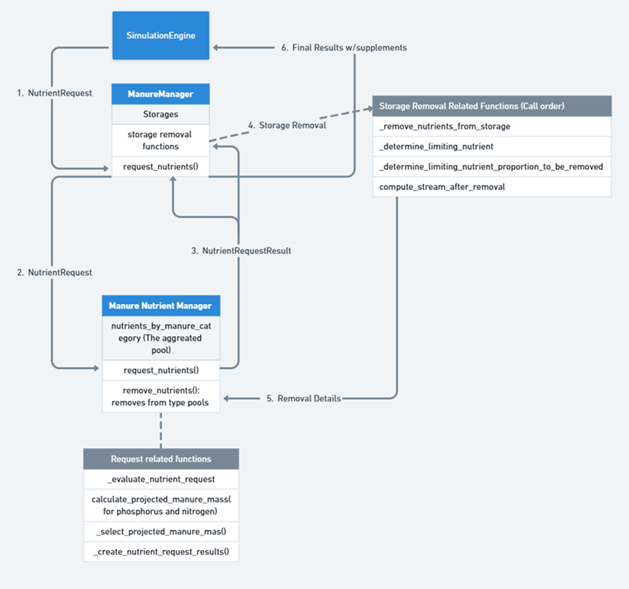
\includegraphics[width=0.9\textwidth]{resources/manurenutrreq.png} 
    \caption{}
    \end{figure}

Each day, the SimulationEngine calls the generate\_daily\_manure\_applications() method to check with the FieldManager to see if there is a manure application scheduled and, when there is, pass the manure nutrient request created by the FieldManager to the ManureManager. The ManureManager, in turn, checks with the ManureNutrientManager to see if the manure nutrient request can be fulfilled via the request\_nutrients() in the ManureManager, which calls the evaluate\_nutrient\_request() function from the ManureNutrientManager class. The ManureNutrientManager then evaluates the nutrient request, determines the limiting nutrient to be used, and calculates the amount of each manure nutrient and the total mass that can be provided by the manure in storage using the following logic. At this time, nutrients from all storages are pooled by ManureNutrientManager to determine the total quantity of nutrients available. Once the nutrient request is returned, an identical proportion (not amount) of manure is removed from all storages. In other words, the user cannot specify at this time which storage(s) should be pulled from for a manure application.

\subsection{Methodology}
\textbf{Step 1: Determination of the Limiting Nutrient}
\\
Determine the nutrient that manure storage removal will be based on using the composition of N and P in the manure nutrient pool. This step is executed by evaluate\_nutrient\_request:

\begin{align}
\text{manure\_mass\_N} &= \frac{\text{mass\_N\_requested}}{\text{manure\_nitrogen\_frac}} \\
\\
\text{manure\_mass\_P} &= \frac{\text{mass\_P\_requested}}{\text{manure\_phosphorus\_frac}}
\end{align}

The projected manure mass is then calculated as:
\begin{equation}
\text{projected manure mass} = \min\left( \text{mass\_N\_requested}, \text{mass\_P\_requested} \right)
\end{equation}
\vspace{0.5cm} 
    
    {\raggedleft \textbf{[MN.MSC.1]}\par}
    \vspace{0.5cm}

where:
\begin{itemize}
\item $\text{mass\_N\_requested}$ is the mass of manure (kg) required to meet the requested mass of N.
\item $\text{mass\_P\_requested}$ is the mass of manure (kg) required to meet the requested mass of P.
\end{itemize}

The limiting nutrient is the nutrient (N or P) with a smaller projected mass required to meet the nutrient request. The projected manure mass based on the limiting nutrient is used to determine the removal of manure from the manure storages.

\vspace{0.2cm}
\textbf{Step 2: Proportion of Limiting Nutrient Removed}

Using the limiting nutrient identified in Step 1 and considering the total quantity of that nutrient available in the aggregated ManureNutrient pool, the proportion of the limiting nutrient to be removed from each storage is calculated as:
\begin{equation}
\text{nutrient\_proportion\_to\_be\_removed} =
\min\left(
\frac{\text{mass\_requested\_nutrient}}{\text{manure\_nutrient\_available}},
1
\right)
\end{equation}
\vspace{0.5cm} 
    
    {\raggedleft \textbf{[MN.MSC.2]}\par}

\vspace{0.2cm}
\textbf{Step 3: Removal of Nutrients from Individual Storages}
\\
Next, the amount of the limiting nutrient and projected mass of manure to be removed from the aggregated ManureNutrient pool are determined. If there is sufficient manure available to fulfill the nutrient request, the quantity of the limiting nutrient removed will be equal to the requested amount; otherwise, the amount removed will be lower than the requested amount.
\\
For each nutrient and each storage, the nutrient removal is calculated as:
\begin{equation}
\text{nutrient\_to\_be\_removed\_from\_storage} =
\text{nutrient\_in\_storage} \times \text{nutrient\_proportion\_to\_be\_removed}
\end{equation}
\vspace{0.5cm} 
    
    {\raggedleft \textbf{[MN.MSC.3]}\par}
    \vspace{0.5cm}

where:
\begin{itemize}
\item $\text{nutrient\_to\_be\_removed\_from\_storage}$ is the mass of the nutrient removed from a specific manure storage (kg).
\item $\text{nutrient\_in\_storage}$ is the mass of the nutrient in the storage prior to manure application (kg).
\end{itemize}

The ManureNutrientManager then passes the result of the manure nutrient request with the total amount of the limiting nutrient to be supplied and the ManureManager calculates the mass of manure and nutrients to be removed from each individual storage. The ManureManager returns the final results of the manure application to the SimulationEngine, including:
\begin{itemize}
\item Total nitrogen mass supplied (kg)
\item Total phosphorus mass supplied (kg)
\item Total manure mass supplied (kg)
\item Total dry matter supplied (kg)
\item Dry matter fraction of the manure (\%)
\item A Boolean indicator of whether the nutrient request was fulfilled
\end{itemize}

After the nutrient request is partially or fully fulfilled, the corresponding quantities of mass and nutrients are subtracted from each individual manure storage.

\newpage
\begin{landscape}
\section{Key Constants}
\fancypagestyle{landscapeplain}{
  \fancyhf{}
  \renewcommand{\headrulewidth}{0pt}
  \renewcommand{\footrulewidth}{0pt}
}
\pagestyle{landscapeplain}

\renewcommand{\arraystretch}{1.3}
\newcolumntype{L}[1]{>{\raggedright\arraybackslash}p{#1}}

\begin{longtable}{@{} L{8cm} L{3cm} L{10cm} @{}} 
\caption{The key constants for all equations in the Manure Module} \\
\toprule
\multicolumn{1}{c}{\textbf{Variable}} &
\multicolumn{1}{c}{\textbf{Value}} &
\multicolumn{1}{c}{\textbf{Definition}} \\
\midrule
\endfirsthead

\multicolumn{3}{@{}l}{\textit{Table continued from previous page}} \\
\toprule
\multicolumn{1}{c}{\textbf{Variable}} &
\multicolumn{1}{c}{\textbf{Value}} &
\multicolumn{1}{c}{\textbf{Definition}} \\
\midrule
\endhead

\midrule
\multicolumn{3}{@{}r@{}}{\textit{Continued on next page}} \\
\endfoot

\bottomrule
\endlastfoot

\endlastfoot

MANURE\_DAMPING\_FACTOR & 0.65 & Fixed damping factor applied to the air temperature amplitude. \\
MANURE\_TEMPERATURE\_LAG & 30 & Lag constant representing delayed thermal response of manure temperature relative to air temperature (days). \\
ANAEROBIC\_LAGOON\_MANURE\_RETENTION & 0.1 & Fraction of stored manure retained in anaerobic lagoon when storage interval is reached. \\
ACTIVATION\_ENERGY & 81,000 J/mol & Apparent activation energy of methanogenesis in dairy manure. \\
DEFAULT\_STORED\_MANURE\_PH & 7.5 & Default pH of manure in slurry storage or anaerobic lagoon. \\
FREEBOARD\_CONSTANT & 1.2 & 20\% volume allowance above max volume if surface area not user-defined. \\
DEPTH\_CONSTANT & 4.572 & Depth of slurry/liquid manure storage used for surface area calculation (m). \\
PRECIPITATION\_CONSTANT & 0.25 & Annual precipitation constant for determining storage surface area (m). \\
MANURE\_CONVERSION\_CONSTANT & 0.1175 & Factor to estimate manure volume per cow per day (m\textsuperscript{3}). \\
METHANE\_DESTRUCTION\_EFFICIENCY & 0.81 & Percent methane destroyed with cover and flare system. \\
VS\_TO\_METHANE\_LOSS\_RATIO & 6.665 kg & Mass ratio of CO\textsubscript{2}+CH\textsubscript{4} to CH\textsubscript{4} from storage \parencite{Petersen2024}. \\
NATURAL\_LOG\_ARRHENIUS\_CONSTANT & 30.6 g CH\textsubscript{4}/kg VS/h & Log of Arrhenius parameter for methane emissions from stored manure. \\
STORAGE\_RESISTANCE & 23.1 & Default resistance to ammonia volatilization (s/m). \\
SLURRY\_MANURE\_DENSITY & 990 kg/m\textsuperscript{3} & Default density of manure as excreted. \\
AMMONIA\_EMISSION\_COEFFICIENT\_UNTILLED & 0.25 & Ammonia emission coefficient (no mixing). \\
AMMONIA\_EMISSION\_COEFFICIENT\_TILLED & 0.5 & Ammonia emission coefficient (with mixing). \\
DEFAULT\_DAYS\_SINCE\_LAST\_MIXING & 1 d & Days since last mixing, for C decomposition. \\
NITROUS\_OXIDE\_EMISSION\_UNTILLED & 0.01 & N\textsubscript{2}O-N emitted per kg manure N/day (no mixing). \\
NITROUS\_OXIDE\_EMISSION\_TILLED & 0.07 & N\textsubscript{2}O-N emitted per kg manure N/day (with mixing). \\
HOUSING\_SPECIFIC\_CONSTANT & 260.0 s/m & Default constant for ammonia emissions from housing. \\
DEFAULT\_PH\_FOR\_HOUSING\_AMMONIA & 7.7 & Default pH for manure on housing floors. \\
MILKING\_FRESH\_WATER\_USE\_RATE & 30 L/animal/day & Milking water use rate per animal. \\
WATER\_DENSITY\_KG\_PER\_M3 & 0.997 kg/m\textsuperscript{3} & Default water density. \\
CARBON\_DIOXIDE\_MOLAR\_MASS & 44.01 g/mol & Molar mass of CO\textsubscript{2}. \\
CARBON\_DIOXIDE\_TO\_METHANE\_RATIO & 4–6 & Volumetric ratio of CO\textsubscript{2} to CH\textsubscript{4} during digestion. \\
IDEAL\_GAS\_LAW\_R & 0.0821 L atm/mol K & Ideal gas law constant. \\
METHANE\_MOLAR\_MASS & 16.04 g/mol & Molar mass of CH\textsubscript{4}. \\
TAN\_INCREASE\_FACTOR & 1.60 & TAN increase from anaerobic digestion (unitless). \\
DEFAULT\_LAYER\_TEMPERATURE & 30 \textdegree{}C & Default layer temperature for decomposition. \\
DECOMPOSITION\_TEMPERATURE & 60 \textdegree{}C & Temperature for peak microbial activity. \\
DEFAULT\_CARBON\_FRACTION\_VSD & 0.5 & Carbon content of degradable VS. \\
DEFAULT\_CARBON\_FRACTION\_VSND & 0.35 & Carbon content of non-degradable VS. \\
DEFAULT\_MOISTURE\_EFFECT & 0.65 & Moisture effect on microbial decomposition. \\
DEFAULT\_LAG\_TIME & 2 d & Lag time for C decomposition. \\
EFFECTIVE\_MICROBIAL\_DECOMP\_RATE & 0.00237 & Microbial decomposition rate (unitless). \\
FIRST\_ORDER\_DECAY\_COEFFICIENT & 0.01 & First-order decay coefficient. \\
LEACHING\_COEFFICIENT & -- & N leached per kg manure N/day. \\
DEFAULT\_DAYS\_SINCE\_LAST\_HARROW & 1 d & Days since last harrow event. \\
ACHIEVABLE\_METHANE\_EMISSION & 0.24 m\textsuperscript{3} CH\textsubscript{4}/kg VS & Achievable methane generation. \\
SOLID\_MANURE\_DENSITY & 700 kg/m\textsuperscript{3} & Default solid manure density. \\
LIQUID\_MANURE\_DENSITY & 1000 kg/m\textsuperscript{3} & Default liquid manure density. \\

\end{longtable}
\end{landscape}



\newpage
\section{References}
\label{sec:References for Manure Module}
\printbibliography[heading=subbibliography,title={}]
\end{refsection}

\part{Soil and Crop Module}
% Global Table of Contents
\thispagestyle{fancy}

% Local TOC that includes only what’s inside THIS section
\etocsettocstyle{\subsection*{Contents}}{} % heading for the local toc
\etocsetnexttocdepth{subsection}           % or subsubsection
\localtableofcontents
\newpage

\section*{List of Figures}
\locallistoffigures
\newpage

\section*{List of Tables}
\locallistoftables
\newpage

\section{Module Introduction}
\par\noindent\justifying

The Soil and Crop Module simulates the daily changes in soil composition and crop growth based on nutrient availability, weather and soil types. The underlying biophysical processes are drawn from existing models of soil and plant biogeochemistry including the SWAT model, Daycent, and SurPhos. The management routines execute the daily biogeochemical processes and direct simulation of the user-provided management practices including application of manure or synthetic fertilizer, tillage, planting and harvesting. As part of the whole farm biophysical simulation in RuFaS, the Soil and Crop Module receives manure from the Manure Module and sends harvested crop biomass to the Feed Storage Module.
\vspace{0.2cm}


\section{Field Management}
\subsection{Introduction}
The Field Manager (FieldManager) is analogous to the agronomist or field manager on a real dairy farm. It coordinates and manages all the different routines and processes that are executed in Soil and Crop Module across any number of fields. To start with, the field manager interprets and integrates all of the user’s inputs about field management, crops, and soils to create a set of fields that each have their specified field and soil properties as well as schedules for each of the key management operations (manure application, fertilizer application, tillage, planting, and harvesting). 
\vspace{0.2cm}

Once the fields and their schedules are set up, the FieldManager works through daily updates for each field. These daily updates include:
\begin{itemize}
    \item Gathering the weather conditions for that day
    \item Checking if there is a manure application needed so that it can coordinate with Manure Module to provide the manure for the application
    \item Calling each field’s daily update methods
    \item Recording the harvested crops and sending them to the Feed Storage Module

\end{itemize}

The FieldManager is also responsible for calling functions to record and reset any annual data records or processes for each field. Thus, the FieldManager is responsible for receiving and generating information from the user and other parts of the model and coordinating the simulation within the Soil and Crop Module.

\paragraph{Setting up Field Management}
\vspace{-0.25cm}

RuFaS can simulate as many fields as the user wishes to specify and requires a unique input file for each field. However, individual fields can share soil, crop, and management schedule inputs so that the user can simulate multiple fields with, for example, the same soil configuration but different crop and management schedules or different crops with the same manure application schedules without having to replicate the inputs for fields with shared characteristics.

\paragraph{Field Management Initialization}
\vspace{-0.25cm}

The FieldManager class, implemented in field\_manager.py, has a series of functions to help package the user-provided configuration data and management schedule information required to initialize each field. These functions all start with the prefix “set\_up” and are called by the wrapper function “set\_up\_field().” There is only one instance of the FieldManager class as it is used to set up and coordinate processes across all the fields. The following functions within the FieldManager class gather information and call other functions to help initialize key data classes required for initialization of each field:
\begin{itemize}
    \item “setup\_field\_data”: This function sets up the field data parameters and returns an instance of the FieldData class populated with the values from the field\_configuration\_data 
    \item “setup\_soil\_data”: This function sets up a Soil instance that itself contains a SoilData instance configured to the user-provided specifications
    \item “setup\_soil\_layer\_data”: This function sets up a soil LayerData instance configured with provided data that is added to the SoilData instance
\end{itemize}

See the Individual Field Management section below for more information about the FieldData Class and the Soil submodule documentation for information related to the soil data classes.
\vspace{0.2cm}

The next group of “set\_up” functions in FieldManager help initialize the management schedules for each field. These functions call initialization routines for a schedule class that is used to generate an instance of a schedule with all the information that is specific to each type of management practice for each field. These schedule classes translate the user input into detailed schedules that can be read and interpreted by the FieldManager and instances of RuFaS Fields on a daily basis to determine the operations that need to be simulated each day. The schedule set up functions are:
\begin{itemize}
    \item “set\_up\_fertilizer\_events”:  This function generates fertilizer application event schedules based on the user-provided fertilizer schedule and returns a fertilizer schedule as well as a dictionary with the available fertilizer mixes
    \item “set\_up\_manure\_events”:  This function generates manure application event schedules based on the user-provided manure application schedules and returns a list of the planned manure applications.
    \item “set\_up\_tillage\_events”: This function generates tillage event schedules based on the user-provided tillage schedules and returns a list of the planned tillage events.
    \item “set\_up\_crop\_events”: This function generates all planting and harvest events based on the user-provided crop rotation schedule and returns a list of planting events and a list of the harvesting events that correspond to the planting events. 
    \item “set\_up\_crop\_schedules”: This function is called by set\_up\_crop\_events() and returns a single list of all the cropping schedules.
\end{itemize}

Outputs for each field can be identified by the character string used to define the field input blob in the metadata file. 

For example, in the below excerpt from a metadata input file: 

        \begin{figure}[H] % The 'p' option places the figure on a page by itself
  \centering
  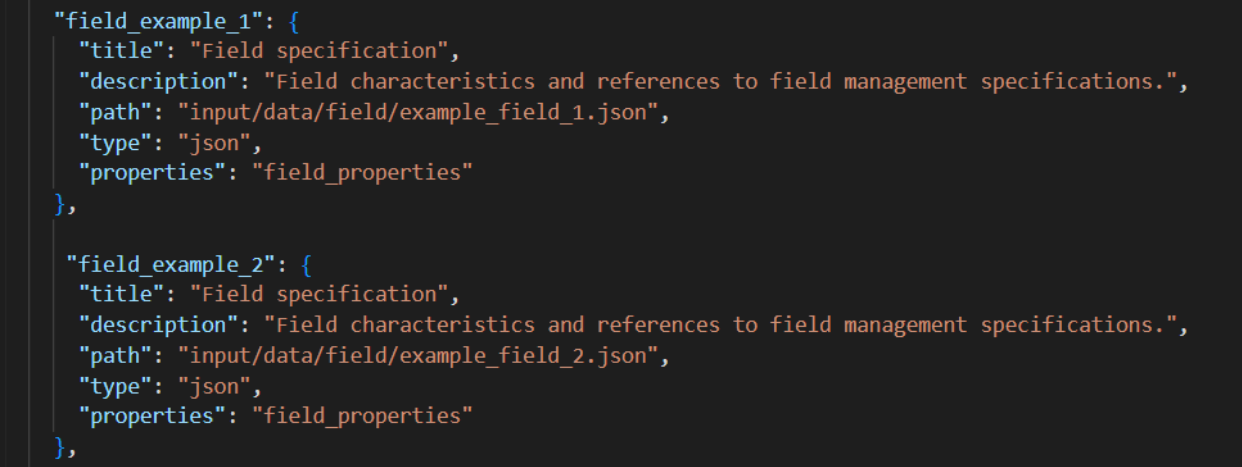
\includegraphics[width=0.9\textwidth]{resources/metadatainput.png} % Replace with your image file
  \caption{Example of the metadata input file.}

\end{figure}




there are 2 different fields named “field\_example\_1” and “field\_example\_2” so the outputs generated by the first field would take the form:

Class.function.variable.field=’field\_example\_1’

Where the pre-fix Class.function.variable is determined by the class, function that produced the variable, and the variable being reported. As a specific illustration, the output variable for the daily surface residue from “field\_example\_1” would be: 

FieldDataReporter.send\_field\_daily\_variables.current\_residue.field='field\_example\_1'

\paragraph{Field Setup and Initialization}
\vspace{-0.25cm}

When directed by the FieldManager, the Field class initializes a new Field object with the user-provided information that is packaged and shared by the FieldManager. These inputs include things like the field location, size, irrigation practices, pointers to the input files with management schedules, and options for turning crop growth stressors on and off. 


\newpage
\begin{landscape}
\paragraph{Required Inputs}
\vspace{-0.25cm}

\fancypagestyle{landscapeplain}{
  \fancyhf{}
  \renewcommand{\headrulewidth}{0pt}
  \renewcommand{\footrulewidth}{0pt}
}
\pagestyle{landscapeplain}

\renewcommand{\arraystretch}{1.3}
\newcolumntype{L}[1]{>{\raggedright\arraybackslash}p{#1}}

\begin{longtable}{@{} L{3.5cm} L{4cm} L{6cm} p{1.2cm} p{1.2cm} p{1.2cm} @{}} 
\caption{Required user inputs for the FieldManager section.} \\

\toprule
\multicolumn{1}{c}{\textbf{Section}} &
\multicolumn{1}{c}{\textbf{Variable}} &
\multicolumn{1}{c}{\textbf{Definition}} &
\multicolumn{1}{c}{\textbf{Default}} &
\multicolumn{1}{c}{\textbf{Min}} &
\multicolumn{1}{c}{\textbf{Max}}\\
\midrule
\endfirsthead

\multicolumn{6}{@{}l}{\textit{Table continued from previous page}} \\
\toprule
\multicolumn{1}{c}{\textbf{Section}} &
\multicolumn{1}{c}{\textbf{Variable}} &
\multicolumn{1}{c}{\textbf{Definition}} &
\multicolumn{1}{c}{\textbf{Default}} &
\multicolumn{1}{c}{\textbf{Min}} &
\multicolumn{1}{c}{\textbf{Max}}\\
\midrule
\endhead

\midrule
\multicolumn{6}{@{}r@{}}{\textit{Continued on next page}} \\
\endfoot

\bottomrule
\endlastfoot

\multirow{9}{*}{\textbf{Field}} 
 & field\_size & Size of the field (ha) & N/A & 0 & NA  \\
 & absolute\_latitude & The absolute latitude of the center of this field.(degrees). & 43.5 & 0 & 90  \\
 & longitude & The longitude of the center of this field (degrees). & -89.4 & -180 & 180  \\
 & watering\_amount\_in\_liters & Amount of water to be applied as irrigation at the end of a specified interval (L). & 0 & 0 & N/A  \\
 & watering\_interval & Number of days that make up the irrigation interval between irrigation events (d). & 0 & 0 & N/A  \\
 & simulate\_water\_stress & Whether water stress affects crops grown in this field. & TRUE & N/A & N/A  \\
 & simulate\_temp\_stress & Whether temperature stress affects crops grown in this field. & TRUE & N/A & N/A  \\
 & simulate\_nitrogen\_stress & Whether nitrogen stress affects crops grown in this field. & TRUE & N/A & N/A  \\
 & simulate\_phosphorus\_stress & Whether phosphorus stress affects crops grown in this field. & TRUE & N/A & N/A  \\

 
\cmidrule(lr){1-6}
\multirow{10}{*}{\textbf{Crop Management}} 
 & crop\_species & Name of the crop being grown. & \multicolumn{3}{p{3.6cm}}{
  \begin{minipage}[t]{3cm}
    \raggedright
    Must be selected from names of configurations defined in the crop configuration input file.
  \end{minipage}
 } \\
 & harvest\_days & Julian day(s) of year to harvest & N/A & 1 & 366  \\
 & harvest\_years & Calendar years in which the harvesting occurs. & N/A & 1 &   \\
 & harvest\_operations & Operation(s) with which this crop will be harvested.  & - & \multicolumn{2}{p{2.4cm}}{
  \begin{minipage}[t]{2.4cm}
    \raggedright
    \begin{itemize}
        \item []
        \item harvest\_only
        \item harvest\_kill
        \item kill\_only
        \item []
    \end{itemize}
  \end{minipage}
 } \\

 & harvest\_type & Whether the crop uses scheduled harvests or optimal harvests (“scheduled”, “optimal”). & scheduled &  &   \\
 & planting\_days & Julian day(s) of year to plant. & N/A & 1 & 366  \\
 & planting\_years & Calendar years in which the planting occurs. & N/A & 1 &   \\
 & pattern\_repeat & Number of times that this crop schedule should be repeated. & 0 & 0 & N/A  \\
 & planting\_skip & Number of years to be skipped between planting schedule repetitions. & 0 & 0 & N/A  \\
 & harvesting\_skip & Number of years to be skipped between harvest schedule repetitions. & 0 & 0 & N/A  \\

\cmidrule(lr){1-6}
\multirow{5}{*}{\textbf{Fertilizer Management}} 
 & name & Name of the fertilizer mix. &  &  &   \\
 & N & Fraction of nitrogen contained in the fertilizer mix by mass. & 1 & 0 & 1  \\
 & P & Fraction of phosphorus contained in the fertilizer mix by mass. & 1 & 0 & 1  \\
 & K & Fraction of potassium contained in the fertilizer mix by mass. & 1 & 0 & 1  \\
 & ammonium\_fraction & Fraction fertilizer nitrogen that is ammonium. All non-ammonium nitrogen is assumed to be nitrate. & 0.5 & 0 & 1  \\
 
\cmidrule(lr){1-6}
\multirow{10}{*}{\textbf{Fertilizer Schedule}} 
 & mix\_names & List of the mix names that will be used for the corresponding fertilizer application. &  &  &   \\
 & years & List of years in which fertilizer will be applied. &  & 1 &   \\
 & days & List of days on which fertilizer will be applied. &  & 1 & 366  \\
 & nitrogen\_masses & List of minimum nitrogen masses that the corresponding fertilizer applications should contain (kg). &  & 0 &   \\
 & phosphorus\_masses & List of minimum phosphorus masses that the corresponding fertilizer applications should contain (kg). &  & 0 &   \\
 & potassium\_masses & List of minimum potassium masses that the corresponding fertilizer applications should contain (kg). &  & 0 &   \\
 & application\_depths & List of depths at which the fertilizer is injected into the soil (mm). &  & 0 &   \\
 & surface\_remainder\_fractions & List of fractions of fertilizer which remain on the soil surface when applied via injection. &  & 0 & 1  \\
 & pattern\_repeat & Number of times that this fertilizer application schedule should be repeated. & 0 & 0 &   \\
 & pattern\_skip & Number of years to be skipped between schedule repetitions. & 0 & 0 &   \\

\cmidrule(lr){1-6}
\multirow{20}{*}{\textbf{Manure Application}} 
 & years & List of years in which tillage will occur. &  & 1 &   \\
 & days & List of days on which tilling will occur. &  & 1 & 366  \\
 & tillage\_depths & List of depths that the corresponding tillage applications reach (mm). &  & 0.1 &   \\
 & incorporation\_fractions & List of fractions of surface pools that get incorporated into the soil during applications. &  & 0 & 1  \\
 & mixing\_fractions & List of fractions of soil layer pools that are available to mix into other soil layers. &  & 0 & 1  \\
 & implements & List of tillage implements which will be used to execute the tillage operations. & -  & \multicolumn{2}{p{2.6cm}}{
  \begin{minipage}[t]{2.6cm}
    \raggedright
    \begin{itemize}
    \item []
      \item subsoiler
      \item moldboard-plow
      \item coulter-chisel-plow
      \item disk-harrow
      \item cultivator
      \item seedbed-conditioner
      \item []
    \end{itemize}
  \end{minipage}
 } \\

 & pattern\_repeat & Number of times that this tillage schedule should be repeated. & 0 & 0 &   \\
 & pattern\_skip & Number of years to be skipped between schedule repetitions. & 0 & 0 &   \\
 & years & List of years in which manure will be applied. &  & 1 &   \\
 & days & List of days on which manure will be applied. &  & 1 & 366  \\
 & nitrogen\_masses & List of minimum nitrogen masses that the corresponding manure applications should contain (kg). &  & 0 &   \\
 & phosphorus\_masses & List of minimum phosphorus masses that the corresponding manure applications should contain (kg). &  & 0 &   \\
 & potassium\_masses & List of minimum potassium masses that the corresponding manure applications should contain (kg). &  & 0 &   \\
 & coverage\_fractions & List of fractions of how much of the field is covered by the corresponding manure application. &  & 0.01 & 1  \\
 & application\_depths & List of depths at which the manure is injected into the soil (kg). &  & 0 &   \\
 & surface\_remainder\_fractions & List of fractions of manure which remain on the soil surface when applied. &  & 0 & 1  \\
 & manure\_types & The type of manure which will be requested for the application. &  &  \multicolumn{2}{p{2.6cm}}{
  \begin{minipage}[t]{2.6cm}
    \raggedright
    \begin{itemize}
    \item []
      \item liquid
      \item solid
      \item []
    \end{itemize}
  \end{minipage}
 } \\

 & supplement\_manure\_ nutrient\_deficiencies & Determines if nutrient deficient manure applications are supplemented with chemical fertilizer. & none  & \multicolumn{2}{p{2.6cm}}{
  \begin{minipage}[t]{2.6cm}
    \raggedright
    \begin{itemize}
    \item []
      \item none
      \item manure
      \item synthetic fertilizer
      \item synthetic fertilizer and manure
      \item []
    \end{itemize}
  \end{minipage}
 } \\

 & pattern\_repeat & Number of times that this manure application schedule should be repeated. & 0 & 0 &   \\
 & pattern\_skip & Number of years to be skipped between schedule repetitions. & 0 & 0 &   \\



\end{longtable}
\end{landscape}



\subsection{Methodology}

The first step to initializing an instance of a field is to initialize an instance of the FieldData class for each field which is called by the setup\_field\_data() function in FieldManager. Each instance of the FieldData class contains key information about the field from the user-provided configuration data that remains fixed throughout the simulation as well as other field attributes that are updated dynamically throughout the simulation such as the amount of crop residue that is on the surface of the field (current\_residue), the amount of water being applied to a field in an irrigation interval (watering\_amount\_in\_mm) and the number of days since the start of the current watering interval (days\_into\_watering\_interval). 
\vspace{0.2cm}

Once the FieldData is initialized, the instances of the SoilData and SoilLayerData classes for that field are initialized.  Following initialization of the soils for each field, the management schedules are generated. The user has some flexibility in how they provide information about the schedule for management operations so that they can either provide a list that provides information and dates for each operation individually, or if the same operation is repeated at an annual timestep or greater, they can provide information about the pattern with which that operation is repeated via the “pattern\_repeat” and “pattern\_skip” inputs. For example, if a user wanted to simulate an operation such as planting corn or fertilizer application that happened every year for 5 years on May 4th starting in 2021, they could specify this schedule with either of the two following combinations of inputs in a management schedule input file:

\textbf{Option 1:}
\begin{itemize}
    \item “years”: [2021, 2022, 2023, 2024, 2025],
    \item “days”: [124, 124, 124, 124, 124],
    \item “pattern\_repeat”: 0, 
    \item “pattern\_skip”: 0
\end{itemize}


\textbf{Option 2:}
\begin{itemize}
    \item “years”: [2021],
    \item “days”: [124],
    \item “pattern\_repeat”: 5, 
    \item “pattern\_skip”: 0
\end{itemize}

Similarly, if a user wanted to simulate something like cover crop planting or a manure application that happened every 4 years on September 5th starting in 1985, they could provide either of the following two inputs for that operation:
\vspace{0.2cm}

\textbf{Option 1:}
\begin{itemize}
    \item “years”: [1985, 1989, 1993, 1997, 2001, 2005],
    \item “days”: [218]],
    \item “pattern\_repeat”: 0, 
    \item “pattern\_skip”: 0
\end{itemize}


\textbf{Option 2:}
\begin{itemize}
    \item “years”: [1985],
    \item “days”: [218],
    \item “pattern\_repeat”: 6, 
    \item “pattern\_skip”: 4
\end{itemize}

To translate the user-provided information about field schedules into standard data formats, RuFaS generates management schedules via operation specific schedule classes. These schedule classes (CropSchedule, FertilizerSchedule, ManureSchedule, and TillageSchedule) are built as child classes from a generic parent class (Schedule) that contains functions to expand the user-provided information about the timing of management operations into a list with a Julian day and year for each management operation alongside any operation specific configuration data. 
\vspace{0.2cm}

\textbf{Crop specific} management data includes specification of both the planting and harvesting schedule, and whether the harvest operation is a harvest only operation (meaning that the crop continues to grow after harvest) or if it is an event that kills the plant, with or without harvesting the crop. 
\vspace{0.2cm}

\textbf{Tillage specific} management information includes the depth of the tillage operation, the amount of surface soil that is mixed into lower parts of the soil profile (incorporation\_fractions), and the amount of mixing that occurs between soil layers (mixing\_fractions). 
\vspace{0.2cm}

\textbf{Fertilizer application specific} management information includes the proportions of N, P, and K in the fertilizer mixes being used, the proportion of N that is in the form of ammonium (ammonium\_fraction), the total masses of N, P, and K applied at each application, the application depth, and the fraction of manure that remains on the surface (surface\_remainder\_fraction). 
\vspace{0.2cm}

\textbf{Manure application specific} management information includes the total masses of N, P, and K applied at each manure application, the application depth, and the fraction of fertilizer that remains on the surface (surface\_remainder\_fraction), and an indication of how the model should handle cases where there is not enough manure in storage to meet the manure application request (supplement\_manure\_nutrient\_deficiencies). 
\vspace{0.2cm}

After the user information about the management schedules are translated into complete lists where each list entry is the schedule information for each operation for the entire simulation, these multi-year schedules are then translated into lists where each entry is an individual event for each operation so that the field manager can iterate over this list. The lists of events are then combined with the field and soil data to initialize an instance of a field!

\paragraph{Daily Field Management}
\vspace{-0.25cm}

Each day the main simulation engine calls on the FieldManager routine to run its daily\_update\_routine() function which returns a list of harvested crops that can be passed to the Feed Storage Module. The FieldManager daily\_update\_routine() function collects the current weather conditions and manure for application to the field where appropriate and calls the Field class manage\_field() routine which is the primary method in the Field class that steps through all the functions that execute the field management operations. The order of operations called is:
\begin{itemize}
    \item Fertilizer Application
    \item Manure Application
    \item Tillage
    \item Soil Nutrient Cycling + Crop Growth
    \item Crop Management
    \begin{itemize}
        \item Transition crops to dormancy
        \item Plant crops
        \item Harvest crops
        \item Update crop and crop residue coverage
    \end{itemize}
\end{itemize}


Once these daily processes have been executed for each field, the FieldManager daily\_update\_routine() function sends all the outputs to the OutputManager via the output\_gatherer.send\_daily\_variables() function. 

\paragraph{Fertilizer Application}
\vspace{-0.25cm}

The first step in execution of a fertilizer application is to calculate the total mass of fertilizer required to meet the minimum N, P, and K application masses requested for each fertilizer given the specified nutrient composition of the fertilizer mix using the following two methods:
            \vspace{0.5cm}        
    
    \begin{center}
        \(fert\_mass_{nitrogen}=\frac{mass\_requested\_nitrogen}{fert\_nitrogen\_frac
fert\_mass}\) \\ 
        \(fert\_mass_{phosphorus}=\frac{mass\_requested\_phosphorus}{fert\_phosphorus\_frac}\) \\
        \(fert\_mass_{potassium}=\frac{mass\_requested\_potassium}{fert\_potassium\_frac}\)
    \end{center}
        \vspace{0.5cm} 
    
            {\raggedleft \textbf{[SC.FLD.1]}\par}
            \vspace{0.5cm} 
    
    \begin{center}
        \(applied\_mass = max[fert\_mass_{nitrogen},\ fert\_mass_{phosphorus}\ fert\_mass_{potassium}] \)
    \end{center}
        \vspace{0.5cm} 
    
            {\raggedleft \textbf{[SC.FLD.2]}\par}
            \vspace{0.5cm} 

\paragraph{Where:}
\begin{itemize}
    \item applied\_mass (kg) is the mass of the given fertilizer required to satisfy all nutrient requests.
    \item fert\_mass\textsubscript{nitrogen} (kg) is the mass nitrogen requested.
    \item fert\_mass\textsubscript{phosphorus} (kg) is the mass of phosphorus requested.
    \item fert\_mass\textsubscript{potassium} (kg) is the mass of potassium requested.
    \item fert\_nitrogen\_frac (proportion) is the fraction of nitrogen in the fertilizer mix.
    \item fert\_phosphorus\_frac (proportion) is the fraction of phosphorus in the fertilizer mix.
    \item fert\_potassium\_frac (proportion) is the fraction of potassium in the fertilizer mix.
\end{itemize}


The mass of each nutrient applied is then calculated as:
            \vspace{0.5cm}        
    
    \begin{center}
        \(applied\_nitrogen=applied\_mass * fert\_nitrogen\_frac\) \\ 
        \(applied\_phosphorus=applied\_mass * fert\_phosphorus\_frac\) \\
        \(applied\_potassium=applied\_mass * fert\_potassium\_frac\)
    \end{center}
        \vspace{0.5cm} 
    
            {\raggedleft \textbf{[SC.FLD.3]}\par}
            \vspace{0.5cm} 

\paragraph{Where:}
\begin{itemize}
    \item applied\_nitrogen (kg) is the mass of nitrogen applied.
    \item applied\_phosphorus (kg) is the mass of phosphorus applied.
    \item applied\_potassium (kg) is the mass of potassium applied.
\end{itemize}
\vspace{0.2cm}

Once the total fertilizer mass and nutrients associated with a fertilizer application are determined, the fertilizer nitrogen and phosphorus masses are added to the appropriate soil nutrient pools via the apply\_fertilizer() function in the FertilizerApplication class in the fertilizer\_application.py file. 
\vspace{0.2cm}

Note that RuFaS does not currently track soil potassium cycling so the application of potassium with fertilizer is recorded solely as a means of tracking resource use. In the future, we hope to add a soil potassium cycling routine at which point potassium will be added to soil nutrient pools via the apply\_fertilizer() method in a similar manner as nitrogen and phosphorus.
\vspace{0.2cm}

Nitrogen and phosphorus are first added to the surface soil layer followed by distribution to the sub-surface layers according to the depth of application. Because soil nutrient pools are tracked in units of kg/ha, the total mass of each nutrient applied to the field is first divided by the field size.
\vspace{0.2cm}


The amount of each nutrient applied to the surface is determined as:
            \vspace{0.5cm} 
    
    \begin{center}
        \(surface\_applied\_nutrient=\frac{(applied\_nutrient * surface\_remainder\_fraction)}{field\_size} \)
    \end{center}
        \vspace{0.5cm} 
    
            {\raggedleft \textbf{[SC.FLD.4]}\par}
            \vspace{0.5cm} 

\paragraph{Where:}
\begin{itemize}
    \item surface\_applied\_nutrient (kg/ha) is the mass per ha of each nutrient applied to the surface soil layer.
    \item surface\_remainder\_fraction (proportion) is the user-provided input defining the fraction of the fertilizer that remains on the soil surface.
    \item field\_size (ha) is the size of the field.
\end{itemize}

The proportion of the subsurface fertilizer that is applied to each layer is calculated from the relationship between the bottom depth of each soil and the application depth. So, for each layer a “depth factor” is calculated as:
\vspace{0.2cm}

if layer\_depth < application\_depth:
            \vspace{0.5cm} 
    
    \begin{center}
        \(depth\_factor=\frac{layer\_depth}{application\_depth} \)
    \end{center}
        \vspace{0.5cm} 
    
            {\raggedleft \textbf{[SC.FLD.5]}\par}
            \vspace{0.5cm} 
else
            \vspace{0.5cm} 
    
    \begin{center}
        \(depth\_factor=1.0-depth\_factor\_sum\)
    \end{center}
        \vspace{0.5cm} 
    
            {\raggedleft \textbf{[SC.FLD.6]}\par}
            \vspace{0.5cm} 

\paragraph{Where:}
\begin{itemize}
    \item depth\_factor (proportion) is the fraction of subsurface fertilizer added to each soil layer
    \item layer\_depth (mm) is the bottom depth of each sub-surface soil layer
    \item depth\_factor\_sum (proportion) is the sum of the depth factors for all layers above the deepest layer receiving fertilizer
\end{itemize}

Thus, the amount of fertilizer added to each nutrient pool in a sub-surface soil layer is: 
            \vspace{0.5cm} 
    
    \begin{center}
        \(sub\_surface\_applied\_nutrient=\frac{(applied\_nutrient * (1- surface\_remainder\_fraction))}{field_size}\)
    \end{center}
        \vspace{0.25cm} 

    \begin{center}
        \(sub\_surface\_applied\_nutrient_{layer\_i}=sub\_surfaapplied\_nutrient * depth\_factor\)
    \end{center}
        \vspace{0.25cm} 

The soil nutrient pools that receive nitrogen are the soil nitrate and ammonium pools. The proportion of fertilizer nitrogen distributed to each of these pools is determined by the user provided ammonium\_fraction.
\vspace{0.2cm}

Fertilizer phosphorus is intended to be added to the labile inorganic phosphorus pools to be available for plant uptake. However, phosphorus applied to the surface is not immediately available in this pool and until the first precipitation or irrigation event the phosphorus is gradually sorbed by the soil. Thus, at the time of application, 75\% of surface applied fertilizer P is added to the available phosphorus pool for gradual sorption and 25\% of the surface applied P is added to the recalcitrant pool which is solubilized during rainfall and either added to the labile phosphorus pool or lost through runoff and leaching.
            \vspace{0.5cm} 
    
    \begin{center}
        \(available\_phorphorus\_pool=surface\_applied\_phosphorus * 0.75\)\\		

        \(recalcitrant\_phorphorus\_pool=surface\_applied\_phosphorus * 0.25\)
    \end{center}
        \vspace{0.5cm} 
    
            {\raggedleft \textbf{[SC.FLD.7]}\par}
            \vspace{0.5cm} 

\paragraph{Manure Application}
\vspace{-0.25cm}

When the results of the manure nutrient request are passed into the FieldManager and then to the Field class daily update routine, the manage\_field() function can then execute the manure application with the manure nutrients and amount provided by the ManureModule via the SimulationEngine. If there are any unmet nutrients from the initial, intended application, if the user indicated that these unmet nutrients can be met with synthetic fertilizers, these are supplied by an additional fertilizer application that is initiated by the handle\_unmet\_nutrients() function. 
\vspace{0.2cm}

Once the amount of manure to be applied is known, the apply\_and\_record\_manure\_application() function first adds the water associated with the manure application.The amount of water in the manure application is determined by the total mass of manure applied and the dry matter fraction of the manure:
            \vspace{0.5cm} 
    
    \begin{center}
        \(manure\_applied\_water=\frac{manure\_mass\_applied }{ manure\_dry\_matter\_fraction}\)
    \end{center}
        \vspace{0.5cm} 
    
            {\raggedleft \textbf{[SC.FLD.8]}\par}
            \vspace{0.5cm} 
            
\paragraph{Where:}
\begin{itemize}
    \item manure\_applied\_water (L) is the amount of water applied to the filed with a manure application
\end{itemize}

The amount of water in liters is then converted to the amount in mm by a helper function convert\_liters\_to\_millimeters() . 
\vspace{0.2cm}

After the water is applied, the phosphorus and nitrogen from manure are applied via the apply\_machine\_manure() function in the ManureApplication class which is implemented in manure\_application.py. The manure application process is broken out into the surface application which follows methods described by the SurPhos model \parencite{vadas2007}  and the subsurface application. 

\paragraph{Surface Manure Application}
\vspace{-0.25cm}

During manure application, the amount of manure applied to the surface is assumed to stay on the surface unless it is a liquid manure with a dry matter content less than 15\% in which case infiltration is assumed and the manure nutrients are assumed to be added to the sub-surface layer. Following the methods from the SurPhos model \parencite{vadas2007}, first the manure solids remaining on the soil surface are calculated:
            \vspace{0.5cm} 
    
    \begin{center}
        \(surface\_dry\_matter\_mass=manure\_dry\_matter\_mass * surface\_remainder\_fraction\)
    \end{center}
        \vspace{0.5cm} 
    
            {\raggedleft \textbf{[SC.FLD.9]}\par}
            \vspace{0.5cm} 
            
\paragraph{Where:}
\begin{itemize}
    \item surface\_dry\_matter\_mass (kg) is the amount of manure solids or dry matter that is applied to the soil surface at that application. 
    \item manure\_dry\_matter\_mass (kg) is the amount of manure solids or dry matter that is applied at that application. 
    \item surface\_remainder\_fraction (kg) is the user-provided value for the amount of the manure applied that remains on the surface.
\end{itemize}


\paragraph{Surface Phosphorus Application}
\vspace{-0.25cm}

Phosphorus is then distributed to 4 pools (water extractable inorganic phosphorus, water extractable organic phosphorus, stable inorganic phosphorus, stable organic phosphorus) according to the following methods:
\vspace{0.2cm}

First the fractions of each type of phosphorus are calculated assuming that 55\% of manure phosphorus is water extractable and 75\% of the non-water extractable or stable phosphorus is inorganic: 
            \vspace{0.5cm} 
    
    \begin{center}
        \(water\_extractable\_inorganic\_phosphorus\_fraction =0.50 \) \\
        \(water\_extractable\_organic\_phosphorus\_fraction =0.50 \) \\
        \(stable\_phosphorus\_fraction =1 - (water\_extractable\_inorganic\_phosphorus\_fraction + water\_extractable\_organic\_phosphorus\_fraction)\) \\
        \(stable\_inorganic\_phosphorus\_fraction =0.75 stable\_phosphorus\_fraction  \) \\
        \(stable\_organic\_phosphorus\_fraction =0.25 stable\_phosphorus\_fraction  \) 
    \end{center}
        \vspace{0.5cm} 
    
            {\raggedleft \textbf{[SC.FLD.10]}\par}
            \vspace{0.5cm} 

Then these fractions are multiplied by the total phosphorus applied as well as the product of the infiltration indicator and the surface remainder fraction to obtain the mass of each phosphorus type applied to add the surface or subsurface soil phosphorus layers:
            \vspace{0.5cm} 
    
    \begin{center}
        \(mass\_to\_add\_to\_labile\_phos =total\_phosphorus\_mass (water\_extractable\_inorganic\_phosphorus\_fraction + 0.95 * water\_extractable\_organic\_phosphorus\_fraction + 0.95 * stable\_organic\_phosphorus\_fraction) * soil\_infiltration * surface\_remainder\_fraction \) 
    \end{center}
        \vspace{0.5cm} 
    
            {\raggedleft \textbf{[SC.FLD.11]}\par}
            \vspace{0.5cm} 
    
    \begin{center}
        \(mass\_to\_add\_to\_active\_phos =total\_phosphorus\_mass * stable\_organic\_phosphorus\_fraction * soil\_infiltration * surface\_remainder\_fraction\) 
    \end{center}
        \vspace{0.5cm} 
    
            {\raggedleft \textbf{[SC.FLD.12]}\par}
            \vspace{0.5cm} 

\paragraph{Where:}
\begin{itemize}
    \item mass\_to\_add\_to\_labile\_phos (kg) is the phosphorus that will be added to the surface labile phosphorus pool during that application.
    \item mass\_to\_add\_to\_active\_phos (kg) is the phosphorus that will be added to the surface active phosphorus pool during that application.
    \item total\_phosphorus\_mass (kg) is the total phosphorus applied during that application.
    \item soil\_infiltration is equal to 0.4 if the manure applied is less than 15\% dry matter, and 0 otherwise.
\end{itemize}

The SurPhos manure pool attributes for the manure dry matter mass, moisture factor and field coverage are then updated according to the new field coverage and surface dry matter mass for that application \parencite{vadas2007}.

\paragraph{Surface Nitrogen Application}
\vspace{-0.25cm}

The composition of manure nitrogen is provided by the manure module as the fractions that are in inorganic nitrogen, ammonium nitrogen, and organic nitrogen. These fractions are then distributed to the soil nitrate, ammonium, fresh organic nitrogen, and stable organic nitrogen pools according to the following:
            \vspace{0.5cm} 
    
    \begin{center}
        \(mass\_nitrates\_added = manure\_dry\_matter\_mass * inorganic\_nitrogen\_fraction * \frac{(1-ammonium\_fraction)}{ field\_size}\) \\
        \(mass\_ammonium\_added = manure\_dry\_matter\_mass * inorganic\_nitrogen\_fraction * \frac{(ammonium\_fraction)}{ field\_size}\) \\
        \(mass\_fresh\_organic\_nitrogen\_added = manure\_dry\_matter\_mass * organic\_nitrogen\_fraction * \frac{fresh\_fraction\_of\_organic\_nitrogen }{field\_size}\) \\
        \(mass\_fresh\_organic\_nitrogen\_added = manure\_dry\_matter\_mass * organic\_nitrogen\_fraction * \frac{(1-fresh\_fraction\_of\_organic\_nitrogen) }{field\_size} \) 
    \end{center}
        \vspace{0.5cm} 
    
            {\raggedleft \textbf{[SC.FLD.13]}\par}
            \vspace{0.5cm} 

\paragraph{Where:}
\begin{itemize}
    \item mass\_nitrates\_added (kg N/ha) is the mass of nitrate nitrogen applied to relevant soil layer
    \item mass\_ammonium\_added (kg N/ha) is the mass of ammonium nitrogen applied to relevant soil layer
    \item mass\_fresh\_organic\_nitrogten\_added (kg N/ha) is the mass of fresh organic nitrogen applied to relevant soil layer
    \item mass\_stable\_organic\_nitrogen\_added (kg N/ha) is the mass of stable organic nitrogen applied to relevant soil layer
    \item manure\_dry\_matter\_mass (kg) is the mass of manure dry matter added to the soil layer
    \item ammonium\_fraction (proportion) is the fraction of inorganic nitrogen that is in the form of ammoniacal nitrogen and is provided by the Manure Module
    \item fresh\_fraction\_of\_organic\_nitrogen (proportion) is the fraction of organic nitrogen that is more quickly mineralized and is set to a constant of 0.9286
\end{itemize}

The manure mass that is applied to the surface layer is set to the 100\% of the surface\_dry\_matter\_mass calculated in \textbf{[SC.FLD.9]} if the manure dry matter content is greater than 15\%. For liquid manure when the dry matter content is less than 15\%, infiltration is assumed and the surface application is set to 60\% of the surface\_dry\_matter\_mass from \textbf{[SC.FLD.9]}  and 40\% of the surface\_dry\_matter\_mass is assigned to be added to the first sub-surface layer.

\paragraph{Subsurface Manure Application}
\vspace{-0.25cm}

For manure applications where a fraction or all of the manure is applied below the soil surface (i.e. injection) the sub-surface manure application method is followed for the proportion of the application applied below the soil surface. 

The sub-surface fraction of manure application is simply calculated as:
            \vspace{0.5cm} 
    
    \begin{center}
        \(subsurface\_fraction =1 - surface\_remainder\_fraction \) 
    \end{center}
        \vspace{0.5cm} 
    
            {\raggedleft \textbf{[SC.FLD.14]}\par}
            \vspace{0.5cm} 

to capture all the manure applied that is not accounted for in the surface application methods.This value, along with the manure nitrogen and phosphorus compositions and the total masses of manure applied in each application is passed into the apply\_subsurface\_manure() function. 

Calculation of the manure phosphorus masses to be added to different soil phosphorus pools occurs according to the equations described in \textbf{[SC.FLD.9]}, \textbf{[SC.FLD.10]}, and \textbf{[SC.FLD.11]}. 

Similarly, calculation of the manure N mass to be added to the subsurface layers follows the methods described in \textbf{[SC.FLD.13]}. 

The method for distributing the total\_phosphorus\_mass and manure\_mass\_applied to the subsurface layers multiplies the manure application masses by the subsurface\_fraction calculated in \textbf{[SC.FLD.9]} and depth\_factors calculated using the method described in \textbf{[SC.FLD.5]} and \textbf{[SC.FLD.6]} as in the generic equation below:
            \vspace{0.5cm} 
    
    \begin{center}
        \(nutrient\_mass\_added\_to\_layer = mass\_applied * nutrient\_fraction
subsurface\_fraction * depth\_factor\) 
    \end{center}
        \vspace{0.5cm} 
    
            {\raggedleft \textbf{[SC.FLD.15]}\par}
            \vspace{0.5cm} 


\paragraph{Tillage Application}
\vspace{-0.25cm}

The tillage method mixes nutrient masses from the soil layers to the layers below them and ensures that the nutrients do not get mixed below the bottom of the soil profile.  The till\_soil() function aggregates all the soil nutrient pools needed to be mixed through tillage including: 

\begin{itemize}
    \item "labile\_inorganic\_phosphorus\_content",
   \item "active\_inorganic\_phosphorus\_content",
   \item "stable\_inorganic\_phosphorus\_content",
   \item "nitrate\_content",
   \item "ammonium\_content",
   \item "active\_organic\_nitrogen\_content",
   \item "stable\_organic\_nitrogen\_content",
   \item "fresh\_organic\_nitrogen\_content",
   \item "metabolic\_litter\_amount",
   \item "structural\_litter\_amount",
   \item "active\_carbon\_amount",
   \item "slow\_carbon\_amount",
   \item "passive\_carbon\_amount"
\end{itemize}

It then iterates through these soil nutrient pools and soil layers to redistribute nutrients between the soil pools according to the user provided tillage depth and mixing fraction.


\paragraph{Initiate Daily Biophysical Processes}
\vspace{-0.25cm}

An important step in the Field classes manage\_field() routine is to initiate the updates to the biophysical processes that are managed by the Soil and Crop classes. This is achieved by the execute\_daily\_processes() method and initiates the following processes:
\begin{itemize}
    \item Snow accumulation and melting
    \item Crop residue and canopy cover update
    \item Soil temperature update
    \item Soil water and nutrient cycling updates
    \item Crop growth updates
\end{itemize}

\paragraph{Crop Management}
\vspace{-0.25cm}

In managing the crop cycle, the daily updates called by the Field class first check if the crop is meant to go into a dormant stage. 

After initiating any dormancy where appropriate, the Field class then checks to see if any crops are scheduled to be planted that day. If so, it calls on the Crop class to initialize Crop and ensures that the max\_root\_depth attribute of that crop does not allow its roots to go below the bottom of the soil profile.

The last management practice the Field class checks is the harvesting event schedule. If a harvest event is scheduled for that day, it initiates the harvest method in the Crop class and updates its list of crops to remove the harvested and killed crops from its list of crops. 






\section{Soil Management} 
\subsection{Introduction}
\vspace{0.2cm}

The soil submodule spatially and dynamically models agronomic and biogeochemical processes taking place on the surface of and within the soil profile. It tracks plant roots/residue, hydrological movement, and dissolved/undissolved carbon, nitrogen, and phosphorus cycling. Carbon and nitrogen nutrient cycling and hydrology are based on the SWAT+ model and phosphorus nutrient cycling on the SurPhos model \parencite{vadas2007}. 

\paragraph{Soil Initialization}
\vspace{-0.25cm}

RuFaS can simulate soils of any combination of textures in as many layers delineated by depth as the user wishes to specify. A single soil type and profile can represent all fields in a simulation or can be specific to individual fields. Each specified soil is stored by RuFaS as a SoilData object consisting of a list of LayerData objects that in turn represent a set of variables specific to each layer of soil. At the start of the simulation the user's soil specifications generate the soil layers for each field and pools of water, carbon, nitrogen, and phosphorus are initialized in each layer.


\begin{landscape}
\paragraph{Required Inputs}
\vspace{-0.25cm}


\fancypagestyle{landscapeplain}{
  \fancyhf{}
  \renewcommand{\headrulewidth}{0pt}
  \renewcommand{\footrulewidth}{0pt}
}

\pagestyle{landscapeplain}

\renewcommand{\arraystretch}{1.3}
\newcolumntype{L}[1]{>{\raggedright\arraybackslash}p{#1}} % Supports line wrapping


\begin{longtable}{@{} L{5cm} L{10cm} L{1cm} L{1cm} L{1cm} @{}}
\caption{Required inputs for the Soil section.}\\
\toprule
\multicolumn{1}{c}{\textbf{Variable}} &
\multicolumn{1}{c}{\textbf{Definition}} &
\multicolumn{1}{c}{\textbf{Default}} &
\multicolumn{1}{c}{\textbf{Min}} &
\multicolumn{1}{c}{\textbf{Max}}\\
\midrule
\endfirsthead

\multicolumn{5}{@{}l}{\textit{Table continued from previous page}} \\
\toprule
\multicolumn{1}{c}{\textbf{Variable}} &
\multicolumn{1}{c}{\textbf{Definition}} &
\multicolumn{1}{c}{\textbf{Default}} &
\multicolumn{1}{c}{\textbf{Min}} &
\multicolumn{1}{c}{\textbf{Max}}\\
\midrule
\endhead

\midrule
\multicolumn{5}{@{}r@{}}{\textit{Continued on next page}} \\
\endfoot

\bottomrule
\endlastfoot



second\_moisture \_condition\_parameter & Curve number parameter for average moisture condition equation (unitless) & 85 & 20 & 99 \\
average\_subbasin\_slope & Slope of the field, measured as rise over run (unitless) & 0.05 & 0 &  \\
slope\_length & Slope of the field, measured as rise over run (m) & 50 & 0 &  \\
manning\_roughness\_coefficient & Roughness coefficient for overland flow (unitless) & 0.4 & 0.001 &  \\
 &  &  &  &  \\
support\_practice\_factor & Ratio of soil loss with a specific support practice based on slope characteristics. This value adjusts for terracing, contouring, and stripcropping, and these features are not present in V1, so this value IS NOT used (unitless) & 0.08 &  &  \\
albedo & The ratio of reflected to total incident short-wave solar radiation. Related primarily to soil color and cover (unitless) & 0.16 & 0 & 1 \\
residue\_fresh\_organic \_mineralization\_rate & Fraction of residue that will decompose in a day given optimal conditions (unitless) & 0.05 & 0 &  \\
soil\_evaporation \_compensation\_coefficient & Modifies depth distribution used to meet soil evaporative demand (unitless) & 0.95 & 0.01 & 1 \\
initial\_residue & Residual plant biomass remaining after a crop is harvested (kg h\textsuperscript{-1}) & 0 & 0 &  \\
soil\_layers & The soil layers that this profile contains. Each element of the array should be a `soil\_layer` object &  & 1 &  \\
bottom\_depth & The bottom depth of each soil layer object within the soil\_layers array (mm) &  & 20 & 500 \\
wilting\_point\_water\_concentration & Condition of soil moisture at which soil water becomes unavailable and water held in the soil at a tension of 1.5 Mpa (mm H\textsubscript{2}O/mm soil) & 0.2 & 0 & 0.95 \\
field\_capacity\_water\_concentration & Soil moisture condition at which the soil matric potential is zero or water held by the soil at 0.033 MPa (mm H\textsubscript{2}O/mm soil) & 0.3 & 0 & 0.95 \\
saturation\_point\_water \_concentration & Concentration of water in a layer when it has become saturated (mm H\textsubscript{2}O/mm soil) & 0.5 & 0 & 0.95 \\
saturated\_hydraulic\_conductivity & Measure of ease of water movement through the soil (mm hr-1) & 9.5 & 0.01 & 15 \\
bulk\_density & Ratio of mass of solid particles to total volume of soil (g cm\textsuperscript{-3}) & 1.4 & 1.1 & 1.9 \\
organic\_carbon\_fraction & Fraction of soil weight that is organic carbon at beginning of the simulation. & 0.012 & 0 & 1 \\
clay\_fraction & Fraction of soil mass that is clay (unitless) & 0.225 & 0 & 1 \\
silt\_fraction & Fraction of soil mass that is silt (unitless) & 0.625 & 0 & 1 \\
sand\_fraction & Fraction of soil mass that is sand (unitless) & 0.125 & 0 & 1 \\
rock\_fraction & Fraction of soil mass that is rock (unitless) & 0.013 & 0 & 1 \\
soil\_water\_concentration & Concentration of water in a soil layer at the beginning of the simulation (mm H\textsubscript{2}O/mm soil) & 0.25 & 0 & 0.95 \\
pH & pH of the soil layer (pH) & 7 & 0 & 14 \\
initial\_temperature & Temperature of the layer at the beginning of the simulation (\(^\circ C\)) & 15.05 &  &  \\
initial\_labile\_inorganic \_phosphorus\_concentration & Concentration of labile inorganic phosphorus in the layer at the beginning of the simulation (mg kg\textsuperscript{-1} soil) & null & 0 &  \\
initial\_fresh\_organic \_phosphorus\_concentration & Concentration of initial fresh organic phosphorus in the layer at the beginning of the simulation (mg kg\textsuperscript{-1} soil) & 0 & 0 &  \\
initial\_soil\_nitrate\_concentration & Concentration of nitrate in the layer at the beginning of the simulation (mg kg\textsuperscript{-1} soil) & null & 0 &  \\
initial\_soil\_ammonium\_concentration & Concentration of ammonium in the layer at the beginning of the simulation (mg kg\textsuperscript{-1} soil) & null & 0 &  \\
humus\_mineralization\_rate\_factor & Rate factor for humus mineralization of active organic nutrients (N and P) (unitless) & 0.003 & 0 & 0.003 \\
ammonium\_volatilization \_cation\_exchange\_factor & Controls the rate of ammonia volatilization (unitless) & 0.45 & 0.01 &  \\
 &  &  &  &  \\
denitrification\_rate\_coefficient & Controls the rate of denitrification (unitless) & 1.4 & 0 & 3 \\
denitrification \_threshold\_water\_content & Fraction of field capacity water content above which denitrification takes place. (unitless) & 1 & 0 & 1 \\
residue\_fresh \_organic\_mineralization\_rate & The fraction of residue that will decompose in a day given optimal conditions (unitless) & 0.05 & 0 &  \\



\end{longtable}
\end{landscape}

\subsection{Methodology}
Soil temperature and water content/flow are the main drivers of soil biogeochemical cycling.

\paragraph{Soil Temperature}
\vspace{-0.25cm}

Soil temperature fluctuates diurnally and seasonally and is estimated daily as a function of the previous day’s soil temperature, average annual air temperature, the current day’s soil surface temperature and depth in the soil profile for each soil layer by using the following equations from SWAT 2009 documentation.

    \begin{center}
\(T_{soil}\ (z,\ d_n) = (L * T_{soil,(z,dn-1)})+(1-L) * [df * (T_{aair}-T_{surf}) +T_{surf}]\)
    \end{center}
        \vspace{0.5cm} 
    
            {\raggedleft \textbf{[SC.TMP.1]}\par}
            \vspace{0.5cm}

        \textbf{Where:}
        
        \begin{itemize}
            \item \(T_{soil\ (z, d_n)}\) =	soil temperature \((^\circ C)\) at depth z (mm) and day of the air d\textsubscript{n}
            \item L	=	lag coefficient( ranging from 0.0 to 1.0, default: 0.8) that controls the influence of the previous day’s temperature on the current day’s temperature  

            \item \(T_{soil(z, d_n-1)}\) =soil temperature \((^\circ C)\) at depth z (mm) on previous day
            \item df	= depth factor that quantifies the influence of depth below surface on soil temperature
            \item \(T_{aair}\)	=	Average annual air temperature \((^\circ C)\)
            \item \(T_{surf}\)	=	Daily soil surface temperature \((^\circ C)\) on the day
        \end{itemize}
        \vspace{0.2cm}

    \begin{center}
\(df=\frac{zd}{zd+exp(-0.867-2.078 * zd})\)
    \end{center}
        \vspace{0.5cm} 
    
            {\raggedleft \textbf{[SC.TMP.2]}\par}
            \vspace{0.5cm}
        \begin{itemize}
            \item zd	=	ratio of depth at the center of soil layer to damping depth
        \end{itemize}
        \vspace{0.2cm}

    \begin{center}
\(zd= \frac{z}{dd}	\)
    \end{center}
        \vspace{0.5cm} 
    
            {\raggedleft \textbf{[SC.TMP.3]}\par}
            \vspace{0.5cm}

        \textbf{Where:}
        
        \begin{itemize}
            \item dd	=	damping depth (mm)
            \item z	=	depth at the center of the soil layer (mm)
        \end{itemize}

Damping depth is a function of soil water and max damping depth. \(dd_{max}\)  is the maximum damping depth (mm) to which the temperature wave penetrates and the amplitude decreases to 1/e or 0.37 of its initial value in the soil layers. This is largely dependent on soil thermal conductivity and thermal diffusivity, and is calculated using following equations
        \vspace{0.2cm}

    \begin{center}
\(dd_{max}=1000 + \frac{2500BD}{BD+686\exp(-5.63BD)}\)
    \end{center}
        \vspace{0.5cm} 
    
            {\raggedleft \textbf{[SC.TMP.4]}\par}
            \vspace{0.5cm}

    \begin{center}
\(dd = dd_{max} * exp\{ln (\frac{500}{dd_{max}}) * [\frac{(1-scale)}{(1+scale)}]^2\}\)
    \end{center}
        \vspace{0.5cm} 
    
            {\raggedleft \textbf{[SC.TMP.5]}\par}
            \vspace{0.5cm}
        \begin{itemize}
            \item \(dd_{max}\)	=	maximum damping depth (mm)
            \item scale	=	scaling factor for soil water
        \end{itemize}
            \vspace{0.5cm}

    \begin{center}
\(scale=\frac{SW}{[(0.356-0.144*BD)*Ztot]}\)
    \end{center}
        \vspace{0.5cm} 
    
            {\raggedleft \textbf{[SC.TMP.6]}\par}
            \vspace{0.5cm}

        \textbf{Where:}
        
        \begin{itemize}
            \item BD	=	soil bulk density (g/cm\textsuperscript{3})
            \item SW	=	total soil water in the profile (mm)
            \item Ztot	=	total soil profile depth (mm)
        \end{itemize}

Soil surface temperature is a function of the previous day’s temperature, the amount of ground cover, and the temperature of a bare soil surface. The temperature of a bare soil is calculated as: 
            \vspace{0.5cm}

    \begin{center}
\(T_{bare}=T_{av}+E_{sr}^{\frac{(Tmax-Tmin)}{2}}\)
    \end{center}
        \vspace{0.5cm} 
    
            {\raggedleft \textbf{[SC.TMP.7]}\par}
            \vspace{0.5cm}

        \textbf{Where:}
        
        \begin{itemize}
            \item \(T_{bare}\)	=	Temperature of a bare soil surface (\(^\circ C\)) with no cover
            \item \(T_{av}\)	=	Average daily temperature (\(^\circ C\)) on the day
            \item \(E_{sr}\) =	radiation term
        \end{itemize}
            \vspace{0.5cm}

    \begin{center}
\(E_{sr}=\frac{[Hday * (1-albedo)-14]}{20}\)
    \end{center}
        \vspace{0.5cm} 
    
            {\raggedleft \textbf{[SC.TMP.8]}\par}
            \vspace{0.5cm}

        \textbf{Where:}
        
        \begin{itemize}
            \item \(H_{day}\)	=	daily solar radiation (user input, MJ/\(m^2\)/d)
            \item albedo	=	daily fraction of incoming sunlight that is reflected by a surface
        \end{itemize}

Albedo should be determined by soil type and is set by user input. 
		
The impact of plant and snow cover is quantified as a weighting factor, bcv, given by the maximum of the following two equations:
            \vspace{0.5cm}

    \begin{center}
\(bcv= \frac{plant\_cover}{plant\_cover+exp(7.563-0.0001297) * plant\_cover}\)
    \end{center}
        \vspace{0.5cm} 
    
            {\raggedleft \textbf{[SC.TMP.9]}\par}
            \vspace{0.5cm}

    \begin{center}
\(bcv=\frac{SNOW}{SNOW+exp(6.055-0.3002) * SNOW}\)
    \end{center}
        \vspace{0.5cm} 
    
            {\raggedleft \textbf{[SC.TMP.10]}\par}
            \vspace{0.5cm}

        \textbf{Where:}
        
            
        \begin{itemize}
            \item SNOW	=	snow water content on the current day (mm)	
            \item plant\_cover = Total aboveground plant biomass and residue on the current day (kg per hectare)

        \end{itemize}
            \vspace{0.5cm}

    \begin{center}
\(Tsurf = (bcv * T_{soil,d-1})+ [(1-bcv) * T_{bare}]\)
    \end{center}
        \vspace{0.5cm} 
    
            {\raggedleft \textbf{[SC.TMP.11]}\par}
            \vspace{0.5cm}
            
        \begin{itemize}
            \item Tsurf	=	surface temperature (\(^\circ C\))
        \end{itemize}
\vspace{0.2cm}

Surface temperature is dependent on the previous day’s soil temperature and is calculated before soil temperature on any given day. On the first day of a simulation the default soil temperature is used for \(T_{soil,d-1}\).
\vspace{0.5cm}

\textbf{\large Soil Hydrology}
The soil hydrological processes calculated in RuFaS are limited to infiltration, the downward movement of water through the soil profile, and evapotranspiration, the movement of water from the soil profile into the atmosphere.
\vspace{0.25cm}
\paragraph{Infiltration (implemented in infiltration.py)}
\vspace{-0.25cm}

The Infiltration class is implemented in infiltration.py and calculates both infiltration and runoff. Infiltration is the movement of soil water into and through the soil profile and surface runoff results when application of water to the ground surface exceeds the infiltration rate. Infiltration is calculated as the difference between the amount of water applied to the surface and the amount of surface water run off. Surface water is thus calculated first and then used to calculate soil water infiltration. Soil texture (percentage of sand, silt, and clay), bulk density, presence of pores, pore diameter, and continuity affect the soil infiltration rate. Slow soil infiltration rate results in ponding in the level areas, surface runoff, and erosion in sloping areas. High infiltration rates can lead to nutrient leaching. Surface runoff is estimated using the NRCS curve number method.

Runoff has a minimum of 0 and is calculated as:
            \vspace{0.5cm}

    \begin{center}
\(if R > 0.2S,\ runoff=R-0.2S*2R+0.8S\) \\
\(if\ not,\ runoff=0	\)
    \end{center}
        \vspace{0.5cm} 
    
            {\raggedleft \textbf{[SC.INF.1]}\par}
            \vspace{0.5cm}

        \textbf{Where:}
            
        \begin{itemize}
            \item R	=	daily rainfall (mm H\textsubscript{2}O) 
            \item S	=	retention parameter (mm H\textsubscript{2}O)
        \end{itemize}


S is determined using an empirical value CN (curve number, unitless, user-defined). Three values of CN are used to determine S.
            \vspace{0.5cm}

    \begin{center}
\(CN_1=CN_2-\frac{20 * 100-CN_2}{100-CN_2+exp[2.533-0.0636 * (100-CN_2)]}	\)
    \end{center}
        \vspace{0.5cm} 
    
            {\raggedleft \textbf{[SC.INF.2]}\par}
            \vspace{0.5cm}

    \begin{center}
\(CN_3=CN_2 * exp [0.00673 * (100-CN_2)]\)
    \end{center}
        \vspace{0.5cm} 
    
            {\raggedleft \textbf{[SC.INF.3]}\par}
            \vspace{0.5cm}

        \textbf{Where:}
            
        \begin{itemize}
            \item CN\textsubscript{1}, the first moisture condition, is the wilting point.
            \item CN\textsubscript{2}, the second moisture condition, curve number is user-defined. 
            \item CN\textsubscript{3}, the third moisture condition, is field capacity. 
        \end{itemize}
\vspace{0.2cm}

S is calculated as
            \vspace{0.5cm}

    \begin{center}
 \( S=S_{max} * \{ 1-\frac{SW_{available}} {SW_{available}+exp[w_1- (w_2 * SW_{available})]} \} \)
    \end{center}
        \vspace{0.5cm} 
    
            {\raggedleft \textbf{[SC.INF.4]}\par}
            \vspace{0.5cm}
            
        \begin{itemize}
            \item \(S_{max}\) =	maximum value for S on any given day (mm H\textsubscript{2}O) 
            \item \(SW_{available}\)	=	available soil profile water content (SW - WP) (mm H\textsubscript{2}O)
            \item \(w_{1},\ w_2\) =	shape coefficients
        \end{itemize}
\vspace{0.2cm}

Smax is calculated as:
            \vspace{0.5cm}

    \begin{center}
 \( S_{max}=25.4 * [\frac{1000}{CN_1}-10]	\)
    \end{center}
        \vspace{0.5cm} 
    
            {\raggedleft \textbf{[SC.INF.5]}\par}
            \vspace{0.5cm}

w1 and w2 are calculated as:

    \begin{center}
 \( w_1=ln \{ \frac{FC}{1-(S_3 * S_{max}^{-1})}-FC \}+w_2 * FC	 \)
    \end{center}
        \vspace{0.5cm} 
    
            {\raggedleft \textbf{[SC.INF.6]}\par}
            \vspace{0.5cm}
            

    \begin{center}
 \( w_2= \frac{ln \{ \frac{FC}{1-(S_3 * S_{max}^{-1})}-FC \} -ln \{ \frac{SAT}{1-(2.54 * S_{max}-1)}-SAT \} }{SAT-FC} \)
    \end{center}
        \vspace{0.5cm} 
    
            {\raggedleft \textbf{[SC.INF.7]}\par}
            \vspace{0.5cm}

        \textbf{Where:}
            
        \begin{itemize}
            \item FC	=	amount of water in soil profile at field capacity (mm H\textsubscript{2}O)
            \item SAT	=	amount of water in soil profile at saturation (mm H\textsubscript{2}O)
        \end{itemize}
\vspace{0.2cm}

S3 is calculated as:
            \vspace{0.5cm}
            

    \begin{center}
 \( S_3=25.4 * [\frac{1000}{CN_3}-10]	\)
    \end{center}
        \vspace{0.5cm} 
    
            {\raggedleft \textbf{[SC.INF.8]}\par}
            \vspace{0.5cm}

When the top layer of the soil is frozen (layerTemp \(\leq 2^\circ C\)), S is modified using the following equation: 
            \vspace{0.5cm}
            

    \begin{center}
 \( S_{frz}=S_{max} * [1-exp(-0.000862 * S )]\)
    \end{center}
        \vspace{0.5cm} 
    
            {\raggedleft \textbf{[SC.INF.9]}\par}
            \vspace{0.5cm}
            
Infiltration into the soil is daily rainfall less daily runoff.
            \vspace{0.5cm}
            

    \begin{center}
 \( Infiltration=R-runoff\)
    \end{center}
        \vspace{0.5cm} 
    
            {\raggedleft \textbf{[SC.INF.10]}\par}
            \vspace{0.5cm}


\paragraph{Evapotranspiration}
\vspace{-0.25cm}

Evapotranspiration (ET) is one of the most important hydrological processes of soil water balance in the soil and crop module. It is the sum of all processes by which water moves from the land surface to the atmosphere via soil evaporation, plant canopy transpiration, and sublimation. RuFaS adapts the Hargreaves method \parencite{hargreaves1985} to estimate ET which only requires temperature as an input.
\vspace{0.2cm}

Potential evapotranspiration (PET) is the maximum amount of water that could be removed due to surface evaporation and plant canopy transpiration with no limitation on water availability, while evapotranspiration (ET) is the actual amount of water lost due to evaporation and transpiration. 
\vspace{0.5cm}

\paragraph{Potential Evapotranspiration  (Implemented in field.py)}  is the larger of 0.001 or function of the radiation, daily temperature range, and heat of vaporization

    \begin{center}
 \( ET_{max}=\max\{\frac{0.0023 * H_0 * (T_{max} - T_{min})^{0.5} * (T_{avg} + 17.8))}{LHV},0.001\} \)
    \end{center}
        \vspace{0.5cm} 
    
            {\raggedleft \textbf{[SC.EVP.1]}\par}
            \vspace{0.5cm}

        \textbf{Where:}
            
        \begin{itemize}
            \item LHV	=	latent heat of vaporization (MJ kg\textsuperscript{-1})
            \item ET\textsubscript{max}	=	potential evapotranspiration (otherwise known as PET) (mm d\textsuperscript{-1})
            \item H\textsubscript{0}	=	extraterrestrial radiation (MJ m\textsuperscript{-2} d\textsuperscript{-1}), input
            \item T\textsubscript{max}	=	maximum air temperature for a given day (\(^\circ C\))
            \item T\textsubscript{min}	=	minimum air temperature for a given day (\(^\circ C\))
            \item T\textsubscript{avg}	=	mean air temperature for a given day (\(^\circ C\))
        \end{itemize}
\vspace{0.2cm}

LHV is calculated as:

    \begin{center}
 \( LHV=2.501-2.361 * 10\textsuperscript{-3} * T\textsubscript{avg} \)
    \end{center}
        \vspace{0.5cm} 
    
            {\raggedleft \textbf{[SC.EVP.2]}\par}
            \vspace{0.5cm}



Maximum crop transpiration (implemented in water\_dynamics.py) is the proportion of potential evapotranspiration that is transpired through the plant canopy. LAI lower than 3.0 and available water in the rooting zone limit transpiration.

    \begin{center}
 \( trans_{max}=\frac{ET_{max} * LAI_{act}}{3.0}	\ \ \ \ \ \ \ \ \ \ \ \ \ \ \ if 0 \leq LAI_{act} \leq 3.0 \) \\
  \(trans_{max}=ET_{max}	\ \ \ \ \ \ \ \ \ \ \ \ \ \ \ if LAI_{act} > 3.0\)
    \end{center}
        \vspace{0.5cm} 
    
            {\raggedleft \textbf{[SC.EVP.3]}\par}
            \vspace{0.5cm}

        \textbf{Where:}
            
        \begin{itemize}
            \item Trans\textsubscript{max}	=	maximum transpiration on a given day (mm H\textsubscript{2}O)
            \item LAI\textsubscript{act}		=	LAI (Leaf Area Index) actual (calculated in Crop Growth)
        \end{itemize}
\vspace{0.2cm}


Sublimation and soil evaporation (implemented in field.py) refer to the phase changes of solid and liquid water to gas which transfer water from land to atmosphere.

    \begin{center}
 \( evap_{max}=ET_{max} * SoilCov\)
    \end{center}
        \vspace{0.5cm} 
    
            {\raggedleft \textbf{[SC.EVP.4]}\par}
            \vspace{0.5cm}

        \textbf{Where:}
            
        \begin{itemize}
            \item evap\textsubscript{max}=	maximum soil evaporation/sublimation on a given day (mm H\textsubscript{2}O)
            \item SoilCov	=	soil cover index
        \end{itemize}
    \vspace{0.2cm}

    \begin{center}
 \(SoilCov=exp(-5.0 * 10^{-5} * BioMass)	\)
    \end{center}
        \vspace{0.5cm} 
    
            {\raggedleft \textbf{[SC.EVP.5]}\par}
            \vspace{0.5cm}

        \textbf{Where:}
            
        \begin{itemize}
            \item BioMass = aboveground biomass and residue (kg ha\textsuperscript{-1}) 
        \end{itemize}
    \vspace{0.2cm}

Potential evaporation is adjusted based on trans\textsubscript{max} as: 
    \vspace{0.2cm}

    \begin{center}

\[
evap_{\text{max}} = min\left\{ \frac{evap_{\text{max}} \cdot ET_{\text{max}}}{evap_{\text{max}} + trans_{\text{max}}},\ evap_{\text{max}} \right\}
\]


    \end{center}
        \vspace{0.5cm} 
    
            {\raggedleft \textbf{[SC.EVP.6]}\par}
            \vspace{0.5cm}

Partition evaporation within soil profile (implemented in evaporation.py) vertically subsets the maximum evaporation to calculate evaporation demand within each layer of the soil profile
\vspace{0.5cm}

    \begin{center}
 \(evap_z=evap_{max} * [\frac{z}{z + exp(2.374-0.00713* z)}]\)
    \end{center}
        \vspace{0.5cm} 
    
            {\raggedleft \textbf{[SC.EVP.7]}\par}
            \vspace{0.5cm}

        \textbf{Where:}
            
        \begin{itemize}
            \item evap\textsubscript{z}	=	evaporation demand at depth z (mm H\textsubscript{2}O)
            \item z	=	depth below soil surface (mm)
        \end{itemize}
    \vspace{0.2cm}

The evaporation demand for a given soil layer is the difference between evaporation demands at the top and bottom of the layer. 
\vspace{0.5cm}

    \begin{center}
 \(evap_{ly}=evap_{bottom}-evap_{top}\)
    \end{center}
        \vspace{0.5cm} 
    
            {\raggedleft \textbf{[SC.EVP.8]}\par}
            \vspace{0.5cm}

When the water content of a soil layer is below field capacity, the
evaporative demand for the layer is reduced according to the following equation
\vspace{0.5cm}

    \begin{center}
 \(evap_{ly}\_reduced=evap_{ly} * exp[2.5 * \frac{SW-FC}{FC-WP}]\ \ \ \ \ \ \ if\ SW<FC\)
    \end{center}
        \vspace{0.5cm} 
    
            {\raggedleft \textbf{[SC.EVP.9]}\par}
            \vspace{0.5cm}

        \textbf{Where:}
            
        \begin{itemize}
            \item evap\textsubscript{ly}	=	evaporation demand of the layer
            \item SW	=	soil water content for the layer (mm H\textsubscript{2}O)
            \item WP	=	soil water content held at wilting point (mm H\textsubscript{2}O)
            \item FC	=	field capacity for soil water (mm H\textsubscript{2}O)
        \end{itemize}
    \vspace{0.2cm}

In addition, the daily amount of water removed by evaporation is limited to 80\% of the plant available water (SW-WP): evaporation.py
\vspace{0.5cm}

    \begin{center}

\[
evap_{ly} = min\left\{ 0.8 * SW-WP,\ evap_{ly} \right\}
\]

 
    \end{center}
        \vspace{0.5cm} 
    
            {\raggedleft \textbf{[SC.EVP.10]}\par}
            \vspace{0.5cm}

The total actual amount of water lost in evapotranspiration (ETact) is equal to the sum of evaporation from each layer

\paragraph{Percolation (implemented in percolation.py)}


Percolation is the process of water movement downward through the soil profile. When the soil water content in a layer is less than or equal to field capacity no percolation occurs. Percolation is not calculated for frozen layers.  \vspace{0.5cm}

    \begin{center}
 \(perc=SW_{perc} * [1-exp(\frac{-t}{TT})]\)
    \end{center}
        \vspace{0.5cm} 
    
            {\raggedleft \textbf{[SC.PER.1]}\par}
            \vspace{0.5cm}

        \textbf{Where:}
            
        \begin{itemize}
            \item SWperc	=	water available for percolation (mm H\textsubscript{2}O)
            \item perc		=	amount of water that percolates to the underlying soil layer (mm H\textsubscript{2}O)
            \item t		=	time step (24 h)
            \item TT =	travel time for percolation (h)

        \end{itemize}
    \vspace{0.2cm}

    \begin{center}
 \(SW_{perc}=SW-FC \ \ \ \ \ \ \ \ \ \ \ \ \ \ \ \ if SW>FC\)
    \end{center}
        \vspace{0.5cm} 
    
            {\raggedleft \textbf{[SC.PER.2]}\par}
            \vspace{0.5cm}
            
TT for each soil layer is calculated as:
 \vspace{0.5cm}

    \begin{center}
 \(TT=\frac{SAT-FC}{Ksat}	\)
    \end{center}
        \vspace{0.5cm} 
    
            {\raggedleft \textbf{[SC.PER.3]}\par}
            \vspace{0.5cm}

        \textbf{Where:}
            
        \begin{itemize}
            \item Ksat	=	saturated hydraulic conductivity (mm/h)
            \item 	SAT     =   Amount of water in the soil layer when completely saturated (mm H\textsubscript{2}O)
        \end{itemize}
\vspace{0.5cm}

\subsection{Soil Erosion (Implemented as  soil\_erosion.py)}
\vspace{0.2cm}

Soil erosion is a geological process whereby surface soil is removed by water/wind and  anthropogenically. In RuFaS, erosion is modeled from individual crop fields using the Modified Universal Soil Loss Equations (MUSLE, SWAT 2009 documentation). The MUSLE input variables include rainfall (rainfall amount and intensity), soil erodibility factor, soil cover/management, best management practices, and the topographic factor.
 \vspace{0.5cm}

 \paragraph{Base Equation, Rainfall Intensity, and Peak Runoff}

    \begin{center}
 \(sed=11.8 *( Qsurf*qpeak*field\_size)^{0.56} * K * C * P * LS * CFRG\)
    \end{center}
        \vspace{0.5cm} 
    
            {\raggedleft \textbf{[SC.ERO.1]}\par}
            \vspace{0.5cm}

        \textbf{Where:}
            
        \begin{itemize}
            \item sed		=	sediment yield on a given day (metric tons)
            \item Qsurf		=	surface runoff volume (m\textsuperscript{3})
            \item qpeak	 	=	peak runoff rate (m\textsuperscript{3}/sec)
            \item field\_size =	Area of the cropping field (ha)
            \item K		=	USLE soil erodibility factor (Mg MJm\textsuperscript{-1}mmm\textsuperscript{-1}))
            \item C		=	USLE cover and management factor
            \item P		=	USLE support practice factor
            \item LS		=	USLE topographic factor
            \item CFRG  = the coarse fragment factor
        \end{itemize}
    \vspace{0.5cm}

q\textsubscript{peak} is calculated as:
 \vspace{0.5cm}

    \begin{center}
 \(qpeak=\frac{RC*I*Area}{3.6}	\)
    \end{center}
        \vspace{0.5cm} 
    
            {\raggedleft \textbf{[SC.ERO.2]}\par}
            \vspace{0.5cm}

        \textbf{Where:}
            
        \begin{itemize}
            \item RC	=	runoff coefficient
            \item 	I	=	rainfall intensity (mm/hr)
            \item 	Area	=	field size (ha)
        \end{itemize}
    \vspace{0.5cm}

RC is the fraction of daily runoff to daily precipitation   
 \vspace{0.5cm}

    \begin{center}
 \(RC=\frac{runoff}{R}\)
    \end{center}
        \vspace{0.5cm} 
    
            {\raggedleft \textbf{[SC.ERO.3]}\par}
            \vspace{0.5cm}

        \textbf{Where:}
            
        \begin{itemize}
            \item runoff	=	runoff (mm H\textsubscript{2}O)
            \item 	R	=	rainfall (mm H\textsubscript{2}O)
        \end{itemize}
    \vspace{0.5cm}

Rainfall intensity is rainfall over time for the time of concentration
 \vspace{0.5cm}

    \begin{center}
 \(I=\frac{Rtc}{Tconc}\)
    \end{center}
        \vspace{0.5cm} 
    
            {\raggedleft \textbf{[SC.ERO.4]}\par}
            \vspace{0.5cm}

        \textbf{Where:}
            
        \begin{itemize}
            \item Rtc	=	rain amount during time of concentration (mm H\textsubscript{2}O)
            \item Tconc	=	time of concentration (h)
        \end{itemize}
    \vspace{0.5cm}

    \begin{center}
 \(Tconc=\frac{Length^{0.6} * n^{0.6}}{18 * slope^{0.3}}\)
    \end{center}
        \vspace{0.5cm} 
    
            {\raggedleft \textbf{[SC.ERO.5]}\par}
            \vspace{0.5cm}

        \textbf{Where:}
            
        \begin{itemize}
            \item Length	=	slope length of field (m)
            \item n	=	manning’s roughness coefficient (Refer Table 2)
            \item slope	=	field slope (m/m)
        \end{itemize}
    \vspace{0.5cm}

    \begin{center}
 \(Rtc=alpha*R\)
    \end{center}
        \vspace{0.5cm} 
    
            {\raggedleft \textbf{[SC.ERO.6]}\par}
            \vspace{0.5cm}

        \textbf{Where:}
            
        \begin{itemize}
            \item alpha	=	fraction of daily rain during time of concentration
        \end{itemize}
    \vspace{0.5cm}

    \begin{center}
 \(alpha=1-exp[2 * Tconc * ln(1-alpha_{0.5})]\)
    \end{center}
        \vspace{0.5cm} 
    
            {\raggedleft \textbf{[SC.ERO.7]}\par}
            \vspace{0.5cm}

        \textbf{Where:}
            
        \begin{itemize}
            \item alpha\textsubscript{0.5}	= fraction of daily rain in in ½ hour of highest intensity
        \end{itemize}
    \vspace{0.5cm}

    \begin{center}
 \(alpha_{0.5}= \frac{\{0.02083+[1-exp(\frac{-125}{R+5})]\}}{2}	\)
    \end{center}
        \vspace{0.5cm} 
    
            {\raggedleft \textbf{[SC.ERO.8]}\par}
            \vspace{0.5cm}

Soil erodibility factor K is calculated as:
    \vspace{0.5cm}

    \begin{center}
 \(K=f_{csand} * f_{cl-si} * f_{orgc} * f_{sand}\)
    \end{center}
        \vspace{0.5cm} 
    
            {\raggedleft \textbf{[SC.ERO.9]}\par}
            \vspace{0.2cm}

        \textbf{Where:}
            
        \begin{itemize}
            \item F\textsubscript{csand}	=	gives low factors for soils with high sand contents and high values for soils with little sand
            \item F\textsubscript{cl-si}	=	gives low factors for soils with high clay to silt ratios
            \item F\textsubscript{orgc}	=	reduces soil erodibility for soils with high organic carbon content
            \item F\textsubscript{sand}	=	reduces soil erodibility for soils with high sand contents
        \end{itemize}
    \vspace{0.5cm}

Factors are calculated as: 
    \vspace{0.5cm}

    \begin{center}
 \(f_{csand}=0.2+0.3*exp[-0.256 * sand * (1-\frac{silt}{100})]	\)
    \end{center}
        \vspace{0.5cm} 
    
            {\raggedleft \textbf{[SC.ERO.10]}\par}
            \vspace{0.5cm}

    \begin{center}
 \(f_{cl-si}=[\frac{silt}{clay+silt}]^{0.3}		\)
    \end{center}
        \vspace{0.5cm} 
    
            {\raggedleft \textbf{[SC.ERO.11]}\par}
            \vspace{0.5cm}

    \begin{center}
 \(f_{orgc}=1 - \frac{0.25orgC}{orgC + exp(3.72-2.95 * orgC)}\)
    \end{center}
        \vspace{0.5cm} 
    
            {\raggedleft \textbf{[SC.ERO.12]}\par}
            \vspace{0.5cm}

        \textbf{Where:}
            
        \begin{itemize}
            \item orgC	=	organic Carbon percentage for the first soil layer.
        \end{itemize}
            \vspace{0.5cm}

    \begin{center}
 \(f_{sand}=1-\frac{0.7 *(1-\frac{sand}{100}}{(1-\frac{sand}{100})+exp(-5.51+22.9 * (\frac{sand}{100})^{-1})}\)
    \end{center}
        \vspace{0.5cm} 
    
            {\raggedleft \textbf{[SC.ERO.13]}\par}
            \vspace{0.5cm}

The cover and management factor, C, is the ratio of soil loss from land cropped under specified conditions to loss from clean-tilled, continuous fallow. The equation below essentially allows C to vary between 0.8 and 0.05 as:
            \vspace{0.5cm}

    \begin{center}
 \(C=exp\{[ln(0.8)-ln(0.05)] * exp(-0.00115*surface\ residue)+ln(0.05)\}\)
    \end{center}
        \vspace{0.5cm} 
    
            {\raggedleft \textbf{[SC.ERO.14]}\par}
            \vspace{0.5cm}

        \textbf{Where:}
            
        \begin{itemize}
            \item Cover	=	amount of residue and growing biomass covering the soil surface (kg/ha)
            \item 0.05	=	the estimated minimum value for C	
        \end{itemize}
    \vspace{0.2cm}

LS is a topographic factor and is the expected ratio of soil loss per unit area from a field slope to that from a 22.1-m length of uniform 9 percent slope under identical conditions. LS is estimated as:
            \vspace{0.5cm}
            
    \begin{center}
 \(LS= \frac{Lhill}{22.1}^m * [65.41 * \text{sin}^2(alphahill) + 4.56 * \text{sin}(alphahill)+0.065]\)
    \end{center}
        \vspace{0.5cm} 
    
            {\raggedleft \textbf{[SC.ERO.15]}\par}
            \vspace{0.5cm}

        \textbf{Where:}
            
        \begin{itemize}
            \item Lhill		=	hill slope length (user input, m)
            \item Alphahill	=	angle of the hill slope, defined as tan\textsuperscript{-1}(average subasin slope) (user input, m/m)
            \item average subbasin slope = average slope for the hydrological subbasin (user input, m/m)
        \end{itemize}
    \vspace{0.2cm}

The exponent m is calculated as 
            \vspace{0.5cm}
            
    \begin{center}
 \(m=0.6 * [1-exp(-35.835 * average\ subbasin\ slope)]	\)
    \end{center}
        \vspace{0.5cm} 
    
            {\raggedleft \textbf{[SC.ERO.16]}\par}
            \vspace{0.5cm}

The P factor is a user defined support practice factor that reduces erosion. 
\vspace{0.2cm}

If there is snow on the ground, this will heavily affect sediment yield. sed is adjusted for snowfall on the range day \(>\) 350, or day \(<\) 60 as:
            \vspace{0.5cm}
            
    \begin{center}
 \(sed_{snow}=\frac{sed}{exp(\frac{3 * snow\ water\ content}{25.4})}\)
    \end{center}
        \vspace{0.5cm} 
    
            {\raggedleft \textbf{[SC.ERO.17]}\par}
            \vspace{0.5cm}

        \textbf{Where:}
            
        \begin{itemize}
            \item sedsnow = snow adjusted sediment yield.
        \end{itemize}
    \vspace{0.2cm}

Coarse Fragment factor (CFRG) is calculated as : 
            \vspace{0.5cm}
            
    \begin{center}
 \(CFRG = exp (-0.053 *  rock)	\)
    \end{center}
        \vspace{0.5cm} 
    
            {\raggedleft \textbf{[SC.ERO.18]}\par}
            \vspace{0.5cm}

        \textbf{Where:}
            
        \begin{itemize}
            \item rock is the percent of rock in the first soil layer
        \end{itemize}
    \vspace{0.5cm}

\subsection{Soil Nitrogen Cycling}
\vspace{0.2cm}


RuFaS tracks soil N as five pools based on nitrogen form and lability. Three pools are organic N; fresh, active, and stable. Two are inorganic N; NH\textsubscript{4}\textsuperscript{+} and NO\textsubscript{3}\textsuperscript{-}. Nitrogen enters the cycle as synthetic fertilizer, manure, and crop residue. Synthetic fertilizers are partitioned into nitrate and ammonium. Manure organic N is partitioned into active and stable organic N pools by 92.86\% and 7.14\% respectively. Active and stable organic N can interconvert. N in the active pool can also get percolated to the second layer. Furthermore, manure dry matter mass goes into ammonium and nitrate pools using certain equations. Residue biomass also gets converted into fresh and active organic N pools via mineralization. If residue is in top 2 cm it goes into the fresh organic N pool while if residue is below 2 cm it goes into the active organic N pool. 80\% of fresh organic N is converted into nitrate and 20\% into active pool via decomposition. Active N is converted into NH\textsubscript{4}\textsuperscript{+} after mineralization. NH\textsubscript{4}\textsuperscript{+} can be converted into NO\textsubscript{3}\textsuperscript{-} via nitrification, taken up by plants, volatilized, percolated, or lost via runoff. NO\textsubscript{3}\textsuperscript{-} can be taken up by plants, percolate, runoff, or denitrify to NO, N\textsubscript{2}O, and N\textsubscript{2} gas.
\vspace{0.5cm}

\textbf{\large Initialize soil N Pools (Implemented in layer\_data.py)}
            \vspace{0.5cm}
            
    \begin{center}
 \(initial\_soil\_nitrate\_concentration=7 * e^{\frac{-depth\_of\_layer\_center}{1000}}\)
    \end{center}
        \vspace{0.5cm} 
    
            {\raggedleft \textbf{[SC.SON.1]}\par}
            \vspace{0.5cm}

        \textbf{Where:}
            
        \begin{itemize}
            \item initial\_soil\_nitrate\_concentration is the initial concentration of nitrate in the soil (mg kg\textsuperscript{-1} or ppm) at depth.
            \item depth\_of\_layer\_center is the depth of the middle of the soil layer from the soil surface (mm).
        \end{itemize}
    \vspace{0.5cm}

The ammonium pool for soil N is initially set by the user in the soil input file.
\vspace{0.2cm}

Organic N values in the soil profile are set by the following equation:
            \vspace{0.5cm}
            
    \begin{center}
 \(humic\_organic\_nitrogen\_concentration =10^4 * \frac{organic\_carbon\_fraction * 100}{14}	\)
    \end{center}
        \vspace{0.5cm} 
    
            {\raggedleft \textbf{[SC.SON.2]}\par}
            \vspace{0.5cm}

        \textbf{Where:}
            
        \begin{itemize}
            \item humic\_organic\_nitrogen\_concentration  is the concentration of humic organic N in the layer (mg kg\textsuperscript{-1} or ppm).
            \item organic\_carbon\_fraction is the percent organic C in the layer (\%, user input).
        \end{itemize}
    \vspace{0.5cm}

Humic organic N is partitioned between the active and stable pools for each layer using the following equations:
\vspace{0.2cm}
            
    \begin{center}
 \(activeN= humic\_organic\_nitrogen\_concentration * FractN\)
 \vspace{0.1cm}
 
 \(stableN =humic\_organic\_nitrogen\_concentration * (1-FractN)	\)
    \end{center}
        \vspace{0.5cm} 
    
            {\raggedleft \textbf{[SC.SON.3]}\par}
            \vspace{0.5cm}

        \textbf{Where:}
            
        \begin{itemize}
            \item activeN, initial\_active\_organic\_nitrogen\_concentration, is the concentration of N in the active organic pool (mg kg\textsuperscript{-1}).
            \item humic\_organic\_nitrogen\_concentration is the concentration of humic organic N in the layer (mg kg\textsuperscript{-1}).
            \item FractN, fraction\_of\_humic\_nitrogen\_in\_active\_pool, is the fraction of humic N in the active pool; General Constant - 0.02.
            \item stableN, initial\_active\_organic\_nitrogen\_concentration, is the concentration of N in the stable organic pool (mg kg\textsuperscript{-1}).
        \end{itemize}
    \vspace{0.5cm}

Fresh N is initialized in the top soil layer only (user defined, usually 0-20 mm), and is 0.15\% of the initial amount of residue on the soil surface.
\vspace{0.2cm}
            
    \begin{center}
 \(fresh\_organic\_nitrogen\_content=0.0015 * residue	\)
    \end{center}
        \vspace{0.5cm} 
    
            {\raggedleft \textbf{[SC.SON.4]}\par}
            \vspace{0.5cm}

        \textbf{Where:}
            
        \begin{itemize}
            \item fresh\_organic\_nitrogen\_content is the fresh organic pool in the top soil layer (kg N ha\textsuperscript{-1}).
            \item residue is material in the residue pool for the top soil layer (kg ha\textsuperscript{-1}).	
        \end{itemize}
    \vspace{0.5cm}

While pool sizes are initialized as concentration (mg kg\textsuperscript{-1}), all calculations are done in units of mass (kg ha\textsuperscript{-1}). The conversion is:
\vspace{0.2cm}
            
    \begin{center}
 \(nitrogen\_mass\_kg\_ha=\frac{(nitrogen\_mass\_mg\_kg * BD * depth * field size)}{field size}\)
    \end{center}
        \vspace{0.5cm} 
    
            {\raggedleft \textbf{[SC.SON.5]}\par}
            \vspace{0.5cm}

     \begin{center}
 \(nitrogen\_mass\_kg\_ha= nitrogen\_mass\_mg\_kg * BD * depth * 10\)
    \end{center}
        \vspace{0.5cm} 
    
            {\raggedleft \textbf{[SC.SON.6]}\par}
            \vspace{0.5cm}

        \textbf{Where:}
            
        \begin{itemize}
            \item BD is the bulk density for the given layer (g cm\textsuperscript{-3} or mg m\textsuperscript{-3} ).
            \item depth is the thickness of a given layer (mm).
            \item field size is the field area (ha).
        \end{itemize}
    \vspace{0.5cm}

All pools have a lower limit of 0. If a transfer of N from one pool to another is greater than the N in the pool of origin, the destination pool receives only the amount that depletes the pool of origin. The rest of the N cycle is in the nitrogen\_cycling folder and run by nitrogen\_cycling.py, which is called from the soil routine.

\paragraph{Nitrification and Volatilization (Implemented in nitirification\_volatilization.py)}

Nitrification is the conversion of  NH\textsubscript{4}\textsuperscript{+} to NO\textsubscript{3}\textsuperscript{-} via microbial oxidation of NH\textsubscript{4}\textsuperscript{+} under suitable soil temperature and moisture conditions. Nitrification occurs only at soil temperatures greater than 5\(^\circ C\) and is modeled as a function of soil temperature and water factors, temp\_factor and water\_factor.
\vspace{0.5cm}
            
    \begin{center}
 \(temp\_factor=min(1.0,\ 0.41\ X\frac{temperature - 5}{10})\ if\ temperature > 5\)
    \end{center}
        \vspace{0.5cm} 
    
            {\raggedleft \textbf{[SC.NNV.1]}\par}
            \vspace{0.5cm}

        \textbf{Where:}
            
        \begin{itemize}
            \item temperature is the temperature in the soil layer (\(^\circ C\)).
        \end{itemize}
    \vspace{0.5cm}

        \textbf{If:}
            
    \begin{center}
 \(water\_content \geq 0.25 * field\_capacity - 0.75 * wilting\_point\)
    \vspace{0.5cm}
	\(water\_factor = 1\)
    \end{center}
        \vspace{0.5cm} 
        
        \textbf{Else:}
            
    \begin{center}
 \(water\_factor=\frac{water\_content - wilting\_point}{0.25*(field\_capacity - wilting\_point)}	\)
    \end{center}
            \vspace{0.5cm}

        \textbf{Where:}
            
        \begin{itemize}
            \item water\_content is the water content of the soil layer on a given day (mm).
            \item field\_capacity is the field capacity water content (mm).
            \item wilting\_point is the wilting point water content (mm).

        \end{itemize}
    \vspace{0.5cm}

The volatilization of aqueous soil ammonium to ammonia gas (NH\textsubscript{3}) occurs even when nitrification does not. NH\textsubscript{3} volatilization is influenced by temperature, moisture, fertilizer application, pH, and depth \parencite{mu-extsoil}.
\vspace{0.5cm}

The volatilization depth factor (DepthFac) is unitless and calculated as:
\vspace{0.5cm}
            
    \begin{center}
 \(depth\_factor=1-\{\frac{depth\_of\_layer\_center}{depth\_of\_layer\_center+exp(4.706-0.0305 * depth\_of\_layer\_center)}\}\)
    \end{center}
        \vspace{0.5cm} 
    
            {\raggedleft \textbf{[SC.NNV.2]}\par}
            \vspace{0.5cm}

        \textbf{Where:}
            
        \begin{itemize}
            \item depth\_of\_layer\_center is the depth from the surface of the soil to the middle of the layer (mm).
        \end{itemize}
    \vspace{0.5cm}

The impact of environmental factors on nitrification and NH\textsubscript{3} volatilization are estimated by nitrification and volatilization regulator equations. Nitrification and volatilization only occur if the soil temperature is greater than 5\(^\circ C\).
\vspace{0.5cm}

A nitrification regulator (nitrification\_regulator) and a volatilization regulator (volatilization\_regulator) are calculated as:
\vspace{0.5cm}
            
    \begin{center}
 \(nitrification\_regulator=temp\_factor * water\_factor \)
 \vspace{0.1cm}

  \(volatilization\_regulator=temp\_factor * depth\_factor * cation\_exchange\_factor\)
    \end{center}
        \vspace{0.5cm} 
    
            {\raggedleft \textbf{[SC.NNV.3]}\par}
            \vspace{0.5cm}

        \textbf{Where:}
            
        \begin{itemize}
            \item cation\_exchange\_factor is provided by the soil input file..
        \end{itemize}
    \vspace{0.5cm}

The total mass of NH\textsubscript{4} (kg N ha\textsuperscript{-1}) converted through nitrification and volatilization is given by:
\vspace{0.5cm}
            
    \begin{center}
 \(total\_ammonium\_lost=NH_4 * [1-exp(-1 *nitrification\_regulator-volatilization\_regulator)]\)
    \end{center}
        \vspace{0.5cm} 
    
            {\raggedleft \textbf{[SC.NNV.4]}\par}
            \vspace{0.5cm}

The estimated fraction of total\_ammonium\_lost that is converted to NO\textsubscript{3} by nitrification is:
\vspace{0.5cm}
            
    \begin{center}
 \(nitrification\_loss\_fraction=1-exp(-1 *nitrification\_regulator)	\)
    \end{center}
        \vspace{0.5cm} 
    
            {\raggedleft \textbf{[SC.NNV.5]}\par}
            \vspace{0.5cm}

The estimated fraction of total\_ammonium\_lost that is lost by volatilization (FracVolatil) is:
\vspace{0.5cm}
            
    \begin{center}
 \(volitilization\_loss\_fraction=1-exp(-1 *volitilization\_regulator)\)
    \end{center}
        \vspace{0.5cm} 
    
            {\raggedleft \textbf{[SC.NNV.6]}\par}
            \vspace{0.5cm}

The amount of N removed from the NH\textsubscript{4} pool via nitrification and converted to NO\textsubscript{3} is (kg N ha\textsuperscript{-1}) calculated as:
\vspace{0.5cm}
            
    \begin{center}
 \(nitrification\_loss=[\frac{nitrification\_loss\_fraction}{nitrification\_loss\_fraction + volitilization\_loss\_fraction}] * total\_ammonium\_lost \)
    \end{center}
        \vspace{0.5cm} 
    
            {\raggedleft \textbf{[SC.NNV.7]}\par}
            \vspace{0.5cm}

        \textbf{If:}
            
    \begin{center}
 \(nitrification\_loss\_fraction+volitilization\_loss\_fraction \leq 0 \)
 \vspace{0.1cm}

 \(nitrification\_loss\ is\ 0 \)
    \end{center}
        \vspace{0.5cm}

\paragraph{N loss in leaching and runoff (Implemented in leaching\_runoff\_erosion.py)}
N can be transported with the movement of water through and out of the soil profile through leaching, runoff, and erosion.  Leaching is the process by which N ions move down the soil profile with percolating soil water (Wang and Li, 2019). Leaching affects inorganic and active organic pools.  If percolation is 0, then percolated N is also 0. NO\textsubscript{3}, NH\textsubscript{4} and active N lost to percolation in each layer is removed from the layer of origin and added to the layer below. The water and N percolated from the bottom layer is lost from the soil profile to the vadose layer. Runoff and erosion N is removed exclusively from the surface soil layer. Lateral flow is not taken into account.
\vspace{0.2cm}

The concentration of NO\textsubscript{3} and NH\textsubscript{4} (kg N mm\textsuperscript{-1} H\textsubscript{2}0) in the mobile water fraction for a given layer (NConc\textsubscript{1}) is: 
\vspace{0.5cm}
            
    \begin{center}
 \(mobile\_water\_nitrogen\_concentration=\frac{NO_3\ or\ NH_4 * [1-exp(\frac{-total\_mobile\_water}{(1- \theta) * SAT})]}{total\_mobile\_water} \)
    \end{center}
        \vspace{0.5cm} 
    
            {\raggedleft \textbf{[SC.NNV.8]}\par}
            \vspace{0.5cm}

        \textbf{Where:}
            
        \begin{itemize}
            \item NO\textsubscript{3} or NH\textsubscript{4} is the amount of nitrate or ammonium in the layer (kg N ha\textsuperscript{-1})
            \item total\_mobile\_water is the amount of mobile water in the layer (mm H\textsubscript{2}O)
            \item \(\theta\) is the fraction of porosity from which anions are excluded
            \item SAT is the saturated water content of the soil layer (mm H\textsubscript{2}O).
        \end{itemize}
    \vspace{0.5cm}

 The amount of mobile water in the layer (mm H\textsubscript{2}O) is the amount of water lost by surface runoff and percolation given as:   
\vspace{0.5cm}
            
    \begin{center}
    for top layer:
 \(total\_mobile\_water=runoff\_water\_amount + percolated\_water\_amount\)

    \end{center}
        \vspace{0.5cm} 
    
            {\raggedleft \textbf{[SC.NNV.9]}\par}
            \vspace{0.5cm}

    \begin{center}
    for lower soil layers:
 \(total\_mobile\_water=percolated\_water\_amount\)

    \end{center}
        \vspace{0.5cm} 
    
            {\raggedleft \textbf{[SC.NNV.10]}\par}
            \vspace{0.5cm}

        \textbf{Where:}
            
        \begin{itemize}
            \item runoff\_water\_amount is the surface runoff generated on a given day (mm H\textsubscript{2}O)
            \item percolated\_water\_amount is the amount of water percolating to the underlying soil layer on a given day (mm H\textsubscript{2}O). 
        \end{itemize}
    \vspace{0.5cm}

The amount/mass (kg N ha\textsuperscript{-1}) of NO\textsubscript{3} and NH\textsubscript{4} lost in surface runoff  is: 
\vspace{0.5cm}
            
    \begin{center}

 \(nitrates\_lost\_to\_runoff=nitrate\_conc\_in\_mobile\_h20 * nitrate\_runoff\_coefficient * runoff\_water\_amount\)
\vspace{0.1cm}

 \(ammonium\_lost\_to\_runoff=ammonium\_conc\_in\_mobile\_h20 * ammonium\_runoff\_coefficient * runoff\_water\_amount\)

    \end{center}
        \vspace{0.5cm} 
    
            {\raggedleft \textbf{[SC.NNV.11]}\par}
            \vspace{0.5cm}

        \textbf{Where:}
            
        \begin{itemize}
            \item xxx\_conc\_in\_mobile\_h20 is the concentration of nitrate or ammonium in the surface layer mobile water (kg N mm\textsuperscript{-1} H\textsubscript{2}O)
            \item xxx\_runoff\_coefficient is the nitrate or ammonium percolation coefficient (GeneralConstants; ammonium = 0.2, nitrate = 0.2)
            \item runoff\_water\_amount is the surface runoff generated on a given day (mm H\textsubscript{2}O) 
        \end{itemize}
    \vspace{0.5cm}

\paragraph{N erosion (Implemented in leaching\_runoff\_erosion.py)}

Soil N is eroded from the organic N pools: fresh, active, and stable.
\vspace{0.5cm}
            
    \begin{center}

 \(nitrogen\_erosion\_concentration= \frac{100 * N(kg N/ha)}{bulk\_density * depth}\)

    \end{center}
        \vspace{0.5cm} 
    
            {\raggedleft \textbf{[SC.LCH.1]}\par}
            \vspace{0.5cm}

        \textbf{Where:}
            
        \begin{itemize}
            \item bulk\_density is the soil layer bulk density (Mg m\textsuperscript{-3})
            \item depth is the thickness of the soil layer (mm).
        \end{itemize}
    \vspace{0.5cm}

Organic N mass loss in erosion (kg N ha\textsuperscript{-1}) is calculated as:
\vspace{0.5cm}
            
    \begin{center}

 \(erosion\_nitrogen\_loss=0.001 * nitrogen\_erosion\_concentration * daily\_soil\_lost  * enrichment\_ratio\)

    \end{center}
        \vspace{0.5cm} 
    
            {\raggedleft \textbf{[SC.LCH.3]}\par}
            \vspace{0.5cm}

        \textbf{Where:}
            
        \begin{itemize}
            \item daily\_soil\_lost is the daily soil loss per hectare (metric tons soil ha\textsuperscript{-1})
            \item nitrogen\_erosion\_concentration  is the concentration of organic N in the top soil layer (g N metric ton\textsuperscript{-1} soil)
            \item enrichment\_ratio is the ratio of concentration of organic N transported with the sediment to that found in the soil surface layer. 
        \end{itemize}
\vspace{0.5cm}
            
    \begin{center}

 \(enrichment\_ratio=exp[1.21-0.16 * log(daily\_soil\_lost  * 1000)]\)

    \end{center}
        \vspace{0.5cm} 
    
            {\raggedleft \textbf{[SC.LCH.4]}\par}
            \vspace{0.5cm}

\vspace{0.5cm}
            
    \begin{center}
 \(Percolated\_ammonium = ammonium\_conc\_in\_mobile\_h20  * percolated\_water\)
 \vspace{0.1cm}

  \(Percolated\_nitrate = nitrate\_conc\_in\_mobile\_h20  * percolated\_water\)
    \end{center}
        \vspace{0.5cm} 
    
            {\raggedleft \textbf{[SC.LCH.5]}\par}
            \vspace{0.5cm}

        \textbf{Where:}
            
        \begin{itemize}
            \item xxx\_conc\_in\_mobile\_h20 is the concentration of nitrate or ammonium in the surface layer mobile water (kg N mm\textsuperscript{-1} H\textsubscript{2}O) as determined in equation \textbf{[SC.NNV.8]}
            \item Percolated\_water is the water percolated from the layer (mm)

        \end{itemize}
    \vspace{0.2cm}

\paragraph{Denitrification (Implemented in denitrification.py)}
Denitrification is the bacterial conversion of NO\textsubscript{3} to denitrified nitrates (N\textsubscript{2}, NO\textsubscript{2}, NO, N\textsubscript{2}O) under anaerobic conditions. The denitrification submodule calculates total denitrified nitrates and partitions these emissions further into N\textsubscript{2}O and N\textsubscript{2}. Denitrification is a function of soil water content, temperature, and induced by the presence of NO\textsubscript{3} and carbon (C). 
\vspace{0.2cm}

The amount of nitrate that is lost to denitrification (DenitrN) (kg N ha\textsuperscript{-1}) is calculated for each soil layer by the function calculate\_denitrification\_amount according to the following equation:
\vspace{0.5cm}
            
    \begin{center}

 If nutrient\_cycling\_soil\_water\_factor\textsubscript{layer[i]}  \(>\)  soil\_water\_threshold:
\vspace{0.5cm}

\(denitrified\_nitrates_{layer[i]} = nitrate\_content_{layer[i]} * max( min( 1.0, 1 - exp(-denitrification\_rate\_coefficient * temp\_factor_{layer[i]} * organic\_carbon\_percent_{layer[i]})),\)

    \end{center}
        \vspace{0.5cm} 
    
            {\raggedleft \textbf{[SC.NDN.1]}\par}
            \vspace{0.5cm}

        \textbf{Else:}
            
        \begin{itemize}
            \item denitrified\_nitrates\textsubscript{layer[i]} = 0

        \end{itemize}
    \vspace{0.2cm}

        \textbf{Where:}
            
        \begin{itemize}
            \item nitrate\_content\textsubscript{layer[i]} is the amount of nitrate in layer i (kg N h\textsuperscript{-1})
            \item denitrification\_rate\_coefficienct is the user defined denitrification rate coefficient which can have values between 0-3 with a default value of 1.4
            \item temp\_factor\textsubscript{layer[i]}  is the nutrient cycling temperature factor for each layer,
            \item organic\_carbon\_percent\textsubscript{layer[i]}  is the amount of organic carbon in the layer (\%) calculated as organic\_carbon\_fraction\textsubscript{layer[i]}  * 100
            \item nutrient\_cycling\_soil\_water\_factor\textsubscript{layer[i]} is the nutrient cycling water factor for the layer i
            \item soil\_water\_threshold is the nutrient\_cycling\_water\_factor threshold value for the soil profile and is a user input with a default of 1.0. According to Wen et al. (2024) the value for the soil\_water\_threshold is typically set to 1.0 so denitrification is allowed to occur when water content is above field capacity.

        \end{itemize}
        \vspace{0.5cm}

The denitrified\_nitrates\textsubscript{layer[i]} is removed from the layer’s NO\textsubscript{3} pool and partitioned into N\textsubscript{2}O and N\textsubscript{2} which are then lost to the atmosphere. 
\vspace{0.2cm}

Partitioning factor is used to partition denitrified nitrates into N\textsubscript{2}O and N\textsubscript{2}
\vspace{0.5cm}
            
    \begin{center}
\(Partitioning\_factor = max((min\ (NO3\_effect, C\_effect) * moisture\_effect *pH\_effect), 0.0)\)
    \end{center}
    \vspace{0.5cm}

            {\raggedleft \textbf{[SC.NDN.2]}\par}
            \vspace{0.5cm}
            
   \begin{center}
\(NO3\_effect=(1.0-[0.5+\text{arctan}(\pi*0.01*\frac{(NO3\_content-190)}{\pi})\}] *25)\)
  \end{center}
    \vspace{0.5cm}

            {\raggedleft \textbf{[SC.NDN.3]}\par}
            \vspace{0.5cm}

   \begin{center}
\(C\_effect=13 +\{\frac{[30.78*\text{arctan}[\pi*0.07*(C_{resp}*1000-13)]}{\pi} \}\)
  \end{center}
    \vspace{0.5cm}

            {\raggedleft \textbf{[SC.NDN.4]}\par}
            \vspace{0.5cm}
            

   \begin{center}
\(moisture\_effect=\frac{1.4}{(13^{17/(13^{(2.2*WFPS)} )} )}\ if\ WFPS=0,\ moisture\ effect = 0 \)
  \end{center}
    \vspace{0.5cm}

            {\raggedleft \textbf{[SC.NDN.5]}\par}
            \vspace{0.5cm}
            

   \begin{center}
\(pH\_effect=\frac{1}{(1470*e^{(-1.1*pH)} )} \)
    \end{center}
    \vspace{0.5cm}

            {\raggedleft \textbf{[SC.NDN.6]}\par}
            \vspace{0.5cm}
            
        
        \textbf{Where:}
            
        \begin{itemize}
            \item NO3\_effect is the effect of nitrate on partitioning (unitless)
            \item C\_effect is the effect of carbon on partitioning (unitless)
            \item arctan= the arc tangents measured in radians of x (values are between -pi/2 and pi/2)
            \item NO3\_content is the amount of nitrate in the layer (ug N/g soil)
            \item C\textsubscript{resp} is carbon respiration from the soil layer (kg ha\textsuperscript{-1})
            \item WFPS is the water filled pore space in the soil layer (unitless). 
        \end{itemize}
        \vspace{0.5cm}

The amount of N\textsubscript{2}O-N emissions (kg N ha\textsuperscript{-1}) are calculated as follows:
\vspace{0.5cm}
            
    \begin{center}
\(nitrous\_oxide\_nitrogen = (\frac{denitrified\_nitrates}{(1 + partitioning_factor)})* 0.001\)
    \end{center}
        \vspace{0.5cm} 
    
            {\raggedleft \textbf{[SC.NDN.7]}\par}
            \vspace{0.5cm}
    \begin{center}
\(N_2(kg)=(\frac{denitrified\_nitrates}{-1(partitioning\_factor)})* 0.001 \)

    \end{center}
        \vspace{0.5cm} 
    
            {\raggedleft \textbf{[SC.NDN.8]}\par}
            \vspace{0.5cm}

        \textbf{Where:}
            
        \begin{itemize}
            \item denitrified\_nitrates is the amount of nitrates that have been denitrified (kg ha\textsuperscript{-1})
        \end{itemize}
        \vspace{0.5cm}

\textit{Mineralization and Decomposition/Immobilization (Implemented in mineralization\_decomp.py)}
\vspace{0.2cm}

Mineralization is the microbial conversion of organic N to simple, soluble forms of organic N (including amino acids) and ultimately to the inorganic N that can be taken up by a plant. Decomposition is the breakdown of fresh organic residue into simpler organic components. Immobilization is the uptake or assimilation of N by microbes making them unavailable (temporarily) to plants. Soil stoichiometry (C:N) determines whether organic N will be mineralized (resulting in more plant available N) or inorganic N will be immobilized (resulting in less plant available N).
\vspace{0.2cm}

The N Mineralization equations represent net mineralization which incorporate immobilization into the equations. Fresh and active N pools are subject to decomposition and mineralization respectively. Mineralization and decomposition are allowed to occur only if soil temperature is greater than 0\(^\circ C\). Soil temperature and water are the two factors used in the mineralization and decomposition equations to account for the impacts of temperature and moisture on these processes. 
\vspace{0.2cm}

N mineralized from the active N pool (Nminact) (kg N ha\textsuperscript{-1}) is calculated as:
\vspace{0.5cm}
            
    \begin{center}
\(N\_min\_active=Min\_rate * (temp\_factor * water\_factor)^{0.5} * activeN\)

    \end{center}
        \vspace{0.5cm} 
    
            {\raggedleft \textbf{[SC.NMN.1]}\par}
            \vspace{0.5cm}

        \textbf{Where:}
            
        \begin{itemize}
            \item humus\_min\_rate is the rate coefficient for mineralization of the humus active organic nitrogen
            \item temp\_factor is the nutrient cycling temperature factor for the layer
            \item water\_factor is the nutrient cycling water factor for the layer
            \item activeN is the amount of N in the active organic pool (kg N ha\textsuperscript{-1}).
        \end{itemize}
        \vspace{0.5cm}

N mineralized from the active pool is transferred from the active pool to the NH\textsubscript{4} pool. Decomposition and mineralization are a function of a daily decay rate constant that is calculated with the C:N and C:P ratios of the residue, and temperature and soil water factors. The C:N and C:P ratios of the residues in the soil layer are currently fixed at:
\vspace{0.5cm}
\begin{center}
\(C:N = 25\)
\(C:P = 200\)
\end{center}
 \vspace{0.5cm}
    {\raggedleft \textbf{[SC.NMN.2]}\par}
    \vspace{0.5cm}

The decay rate constant, the same as that used to calculate residue in crop defines the fraction of residue that is decomposed as: 
\vspace{0.5cm}
            
    \begin{center}
\(decay\_rate\_constant=min\_coeff * residue\_comp\_factor * (temp\_factor * water\_factor)^{0.5}\)
\vspace{0.1cm}

\(ResComp = 1.0\)

    \end{center}
        \vspace{0.5cm} 
    
            {\raggedleft \textbf{[SC.NMN.3]}\par}
            \vspace{0.5cm}

        \textbf{Where:}
            
        \begin{itemize}
            \item residue\_comp\_factor is the nutrient cycling residue composition factor
            \item min\_coeff is the rate coefficient for mineralization of the residue fresh organic nutrients (user-defined, default - 0.05)
            \item temp\_factor is temperature’s effect on nutrient cycling for the layer
            \item water\_factor is water’s effect on nutrient cycling for the layer
        \end{itemize}
        \vspace{0.5cm}
        
Mineralization of the residue fresh organic N (kg N ha\textsuperscript{-1}) is calculated as:
\vspace{0.5cm}
            
    \begin{center}
\(residue\_freshN\_mineralization=decay\_rate\_constant * freshN	\)
\vspace{0.1cm}

\(ResComp = 1.0\)

    \end{center}
        \vspace{0.5cm} 
    
            {\raggedleft \textbf{[SC.NMN.4]}\par}
            \vspace{0.5cm}

        \textbf{Where:}
            
        \begin{itemize}
            \item decay\_rate\_constant is the residue decay rate constant
            \item freshN is the N in the fresh organic pool in the layer (kg N ha\textsuperscript{-1}).
        \end{itemize}
        \vspace{0.5cm}
20\% of the N decomposed from the residue\_freshN\_mineralization is then transferred to the active organic N pool, and 80\% is transferred to the NO\textsubscript{3}  pool. In the top layer, 0.15\% of residue is decomposed into fresh organic N pools.

\textit{Humus Mineralization (Implemented in humus\_mineralization.py)}
\vspace{0.2cm}

In general, the term humus describes the transformed products formed from a wide variety of organic substrates without any intent to assign chemical composition or structure \parencite{hayes2020vindication}. Humus mineralization allows N to move between the active and stable organic pools.  N mineralized from the humus active organic pool is added to the NO\textsubscript{3} pool in the layer. 
\vspace{0.2cm}

The amount of N transferred between the active and stable organic pools (Ntrans) (kg N h\textsuperscript{-1}) maintains an equilibrium, and is calculated as
\vspace{0.5cm}
            
    \begin{center}
\(amount\_transferred=humus\_mineralization\_rate* active\_organic\_nitrogen  *[\frac{1}{fracN}-1]-stable\_organic\_nitrogen \)

    \end{center}
        \vspace{0.5cm} 
    
            {\raggedleft \textbf{[SC.NMN.5]}\par}
            \vspace{0.5cm}

        \textbf{Where:}
            
        \begin{itemize}
            \item humus\_mineralization\_rate is the humus mineralization rate constant 10\textsuperscript{-5}
            \item active\_organic\_nitrogen is the amount of N in the active organic pool (kg N ha\textsuperscript{-1})
            \item fracN is the fraction\_of\_humic\_nitrogen\_in\_the\_active\_ pool (0.02)
            \item stable\_organic\_nitrogen is the amount of N in the stable organic pool (kg N ha\textsuperscript{-1})  
        \end{itemize}
        \vspace{0.5cm}

When Ntrans is positive, N moves from the active to stable organic pool. When Ntrans is negative, N moves from stable to active organic pool.
\vspace{0.5cm}

\subsection{Soil Phosphorus Cycling}
\vspace{0.2cm}


Soil phosphorus cycling is based on the SurPhos model theoretical documentation \parencite{vadas2007}, which identifies eight soil phosphorus pools; two organic and six inorganic. Organic pools are divided into stable and water extractable and inorganic pools are divided into stable, water extractable, active, labile, recalcitrant, and available. RuFaS handles phosphorus cycling via the PhosphorusCycling class, which contains and manages the simulated aspects of phosphorus in a soil profile. These aspects are divided into fertilizer (implemented in fertilizer.py), manure (implemented in manure.py), mineralization (implemented in phosphorus\_mineralization.py), and soluble phosphorus (implemented in soluble\_phosphorus.py). The cycle\_phosphorus method calls each of the daily routines that manage surface and subsurface phosphorus.

\paragraph{Phosphorus Initialization (Implemented in layer\_data.py)}
The P sorption parameter (PSP) is initialized before the simulation begins. The PSP represents how much of any inorganic P added to soil remains labile P upon reaching relative equilibrium. A PSP of 0.5 means 50\% of added P remains labile P and 50\% becomes active P. 
\vspace{0.2cm}

PSP is initialized as:	
\vspace{0.5cm}
            
    \begin{center}
\(PSP= max(0.05,\ min(0.7,\ -0.045 * log(clay) +0.001 * labileP-0.035 * orgC+0.43)\)
    \end{center}
        \vspace{0.5cm} 
    
            {\raggedleft \textbf{[SC.PHO.1]}\par}
            \vspace{0.5cm}
            
    \begin{center}

\( adjusted\_clay\_content= max(10^{-8},\ clay\ fraction*100)\)

    \end{center}
        \vspace{0.5cm} 
    
            {\raggedleft \textbf{[SC.PHO.2]}\par}
            \vspace{0.5cm}

        \textbf{Where:}
            
        \begin{itemize}
            \item PSP is the P sorption parameter (unitless)
            \item clay is the adjusted\_clay\_content 
            \item clay fraction is the fraction of the layer composed of clay
            \item orgC is the percentage of the layer composed of organic carbon, assumed to be 58\% of user-defined organic matter content (\%)
            \item labileP (labile\_inorganic\_phosphorus) is the concentration of labile inorganic phosphorus (mg kg\textsuperscript{-1}) 
        \end{itemize}
        \vspace{0.5cm}
            
    \begin{center}
\(initial\ active\ inorganic\ Pconc=\frac{labile\ inorganic\ P * (1.0 -PSP)}{PSP}	\)
\vspace{0.1cm}

\(initial\ stable\ inorganic\ Pconc=4.0 *activeP\)

    \end{center}
        \vspace{0.5cm} 
    
            {\raggedleft \textbf{[SC.PHO.3]}\par}
            \vspace{0.5cm}

After initialization soil P pools are converted from mg phosphorus kg\textsuperscript{-1} soil to a kg ha\textsuperscript{-1} basis.

\paragraph{Soluble Phosphorus (Implemented in soluble\_phosphorus.py)}

The SolublePhosphorus class calculates the P transferred via hydrological processes in the soil based on equations from the APLE and SurPhos models \parencite{vadas2007}. The daily\_update\_routine alters phosphorus levels in the SoilData object by tracking phosphorus in runoff (if any) from the first soil layer and phosphorus percolated downward through the soil profile.
\vspace{0.2cm}

\paragraph{Soluble Phosphorus Runoff}
        \vspace{0.5cm}
            
    \begin{center}
\(adjusted\ DRP_{runoff}=min(labileP,\ top\_soil\_layerP * extraction\ coefficient * runoff * 10^{-6})\)

    \end{center}
        \vspace{0.5cm} 
    
            {\raggedleft \textbf{[SC.PSL.1]}\par}
            \vspace{0.5cm}

        \textbf{Where:}
            
        \begin{itemize}
            \item adjusted DRPrunoff is the dissolved reactive phosphorus in runoff from the soil (kg ha\textsuperscript{-1}) surface expressed as the lesser of labileP or calculated dissolved P
            \item extraction coefficient is 0.005
            \item Runoff is the amount of water lost from the surface layer (L ha\textsuperscript{-1})
            \item top\_soil\_layerP is:

        \end{itemize}
        \vspace{0.5cm}
            
    \begin{center}
\(top\_soil\_layerP=\frac{labileP * field\_size * kg-to-mg}{bulk\_density * Mg-to-kg * soil\_volume}\)

    \end{center}
        \vspace{0.5cm} 
    
            {\raggedleft \textbf{[SC.PSL.2]}\par}
            \vspace{0.5cm}
            \textbf{Where:}

        \begin{itemize}
            \item labile\_P is the labile phosphorous content of the soil (mg/kg)
            \item field\_size is the field area (hectares)
            \item  kg-to-mg is the constant 10\textsuperscript{6}
            \item Mg-to-kg is the constant 10\textsuperscript{3}
            \item soil\_volume is the volume of soil (m\textsuperscript{3})

        \end{itemize}
        \vspace{0.5cm}

\paragraph{Soluble Phosphorus Leaching}
        \vspace{0.5cm}

Phosphorus leaching is predicted by the clay isotherm function in the APLE documentation \parencite{vadas2007}.
        \vspace{0.5cm}
        
    \begin{center}
\(isotherm\ slope=173.51 * clay\_fraction+8.48\)

    \end{center}
        \vspace{0.5cm} 
    
            {\raggedleft \textbf{[SC.PSL.3]}\par}
            \vspace{0.5cm}

        \textbf{Where:}
            
        \begin{itemize}
            \item soilP is the concentration of P in the soil layer (mg P kg\textsuperscript{-1} soil)
            \item isotherm\_slope is the slope of the isotherm curve (unitless)
            \item clay\_fraction is the fractional clay content of a soil layer (unitless)
        \end{itemize}
        \vspace{0.5cm}
        
    \begin{center}
\(isotherm\_inter=4.726 * isotherm\_slope-8.97\)

    \end{center}
        \vspace{0.5cm} 
    
            {\raggedleft \textbf{[SC.PSL.4]}\par}
            \vspace{0.5cm}

        \textbf{Where:}
            
        \begin{itemize}
            \item isotherm\_inter is the intercept of P sorption isotherm (unitless)
            \item isotherm\_slope is the slope of the P sorption isotherm (unitless)

        \end{itemize}
        \vspace{0.5cm}
        
    \begin{center}
\(DRP_{leachate}=min(20.0,\ exp(\frac{soilP * 1.5-isotherm\_inter}{isotherm\_slope}))\)

    \end{center}
        \vspace{0.5cm} 
    
            {\raggedleft \textbf{[SC.PSL.5]}\par}
            \vspace{0.5cm}

        \textbf{Where:}
            
        \begin{itemize}
            \item DRP\textsubscript{leachate} is the dissolved reactive phosphorus leached from the soil layer (mg L\textsuperscript{-1})
        \end{itemize}
        \vspace{0.2cm}

The maximum leachate concentration specified in APLE is 20 (mg L\textsuperscript{-1}), and is applied here as the min term. Leached P is added to the soil layer immediately below the layer for which it is calculated.
\vspace{0.2cm}

The predicted value in (mg L\textsuperscript{-1}) is then converted to kg h\textsuperscript{-1} and the actual dissolved reactive phosphorus is expressed as the minimum of the layer labile P or the calculated DRP\textsubscript{leachate} to prevent negative values.
        \vspace{0.5cm}
        
    \begin{center}
\(DRP_{leachate},\ actual=min(labileP,\ DRP_{leachate}) \)

    \end{center}
        \vspace{0.5cm} 
    
            {\raggedleft \textbf{[SC.PSL.6]}\par}
            \vspace{0.5cm}

        \textbf{Where:}
            
        \begin{itemize}
            \item DRP\textsubscript{leachate} is the dissolved reactive leachate P (kg ha\textsuperscript{-1})
            \item DRP\textsubscript{leachate},actual is the actual dissolved reactive P leached (kg ha\textsuperscript{-1})
        \end{itemize}
        \vspace{0.2cm}

Summarized leachate values are the sum of values that leave the bottom layer of the soil profile.	
\paragraph{Fertilizer Leaching and Runoff (Implemented in fertilizer.py)}
Simulates the leaching and runoff of phosphorus from fertilizer applied to the soil surface.
\vspace{0.2cm}

\paragraph{Available Fertilizer P pool }
\vspace{0.2cm}

During rainfall events, the fraction of fertilizer P lost is greatest during the first rain event and reduced for each consecutive rainfall event. When synthetic fertilizer P is applied, 75\% of it goes into an available pool, and 25\% goes into a recalcitrant pool. The equation below determines the fraction of P remaining in the available P pool (unitless). 
        \vspace{0.5cm}
        
    \begin{center}
\(fertPavail= max\ (0,\ -0.16 * log(fert_{CNT})+cov)\)

    \end{center}
        \vspace{0.5cm} 
    
            {\raggedleft \textbf{[SC.PSL.7]}\par}
            \vspace{0.5cm}

        \textbf{Where:}
            
        \begin{itemize}
            \item fertP\textsubscript{avail} is the fraction of P remaining in the available P pool
            \item fertCNT	is the number of days since the fertilizer was applied
            \item cov is the cover factor, adjusted based on cover type: 
            \begin{itemize}
                \item “BARE”: 0.5333
                \item “RESIDUE COVER”: 0.6667
                \item “GRASSED”: 0.8
            \end{itemize}
        \end{itemize}
        \vspace{0.2cm}

    \begin{tcolorbox}[colback=white, colframe=black, boxrule=0.5pt, arc=3pt, width=\textwidth]
Note: the multiplicative and additive constants differ between the SurPhos documentation and here, the ones listed here should be preferred \parencite{vadas2007}.
\end{tcolorbox}
\vspace{0.2cm}

fert\textsubscript{CNT} is then iterated to account for the logarithmic curve of fertilizer sorption without rain. The availability of P for runoff or leaching decreases as it sits on the soil surface.
\vspace{0.3cm}

\textit{Runoff and Leaching}
\vspace{0.2cm}     

At the first rainfall event, available P is split between runoff and leachate. Subsequent rain events target the recalcitrant pool, with 40\% of released P leached, and all subsequent events leaching 7.5\% of available P. The partitioning of P between runoff and leachate is a function of the amount of rainfall.
\vspace{0.2cm}
        
    \begin{center}
\(sorp\ \% = rain\_day\_factor\)

    \end{center}
        \vspace{0.5cm} 
    
            {\raggedleft \textbf{[SC.PSL.8]}\par}
            \vspace{0.5cm}

        \textbf{Where:}
            
        \begin{itemize}
            \item rain\_day\_factor is the rain day factor calibrated as described above
        \end{itemize}
        \vspace{0.2cm}


Sorbed fertilizer P is then computed and cannot exceed that in the available P pool:
        \vspace{0.5cm}
        
    \begin{center}
\(fert_{sorp}=min(fertP_{avail},\ max(0.0,\ fertP_{avail} * sorp\ \%))\)
    \end{center}
        \vspace{0.5cm} 
    
            {\raggedleft \textbf{[SC.PSL.9]}\par}
            \vspace{0.5cm}

    \begin{center}
\(fertP_{avail}=fertP_{avail}-fert_{sorp}\)
    \end{center}
        \vspace{0.5cm} 
    
            {\raggedleft \textbf{[SC.PSL.10]}\par}
            \vspace{0.5cm}

    \begin{center}
\(sorp\%= max\ (0,\ -0.16 * log(fert_{CNT})+cov)\)

    \end{center}
        \vspace{0.5cm} 
    
            {\raggedleft \textbf{[SC.PSL.11]}\par}
            \vspace{0.5cm}

        \textbf{Where:}
            
        \begin{itemize}
            \item Fert\textsubscript{sorp} is the fertilizer sorption
        \end{itemize}
        \vspace{0.2cm}

For the first layer, labileP is converted to kg to add adsorbed fertilizer P. labileP is then converted back to kg ha\textsuperscript{-1}. The concentration of fertilizer dissolved P in runoff (mg L\textsuperscript{-1}) (fertP\textsubscript{dissolved in runoff)} is computed:
        \vspace{0.5cm}
        
    \begin{center}
\(fertP_{dissolved\ in\ runoff}=\frac{(fertP * fraction\_P\_released * PD_{fact})}{total\ rainfall}\)
    \end{center}
        \vspace{0.5cm} 
    
            {\raggedleft \textbf{[SC.PSL.12]}\par}
            \vspace{0.5cm}

    \begin{center}
\(PDfact=0.034 * exp(3.4 *(\frac{runoff}{rainfall}))\)

    \end{center}
        \vspace{0.5cm} 
    
            {\raggedleft \textbf{[SC.PSL.13]}\par}
            \vspace{0.5cm}

        \textbf{Where:}
            
        \begin{itemize}
            \item fertP is the amount of fertilizer P in the pool that is going to be leached from (mg)
            \item fraction of P released is the fraction of P solubilized during the current rain event. 1 for first, 0.4 for second, and 0.075 (unitless).
            \item PD\textsubscript{fact} is the P distribution factor is the value that determines P distribution between runoff and infiltration (unitless)
            \item total rainfall is rainfall on the day (L)
        \end{itemize}
        \vspace{0.5cm}

\parencite{vadas2007}
Leached fertilizer P is added to soil labileP for each layer to yield the updated labileP as a function of depth:
        \vspace{0.5cm}
        
    \begin{center}
\(labileP\_updated=labileP+(fert_{leach}-fert_{runoff}) * DF\)

    \end{center}
        \vspace{0.5cm} 
    
            {\raggedleft \textbf{[SC.PSL.14]}\par}
            \vspace{0.5cm}

        \textbf{Where:}
            
        \begin{itemize}
            \item fert\_{leach} is amount of fert P to be leached from one layer to the next
            \item fert\_{runoff} is the amount of fert P lost to runoff
        \end{itemize}
        \vspace{0.5cm}
        
Fertilizer P lost to runoff and leaching are added to their cumulative sums

 \vspace{0.5cm}

\textit{Manure Phosphorus}
\vspace{0.2cm}

Manure is an important source of bioavailable P for crop uptake, runoff, and leaching losses. Organic and inorganic P contributions from manure applications are tracked and modeled, including decomposition of manure solids, labile P release and P sorption. Largely changes to manure P are by three main processes: leaching, decomposition, and assimilation.  



\textit{Manure Phosphorus Leaching (implemented in manure\_pool.py)}
\vspace{0.2cm}
        
    \begin{center}
\(MIP_{leach} = max(0.0, manure_{extr}*WIP) \)
\vspace{0.1cm}

\(MOP_{leach} = max(0.0,\ \frac{manure_{extr}*WOP}{0.6})\)

    \end{center}
        \vspace{0.5cm} 
    
            {\raggedleft \textbf{[SC.PSL.31]}\par}
            \vspace{0.5cm}

        \textbf{Where:}
            
        \begin{itemize}
            \item MIP\textsubscript{leach} is the manure inorganic P leached (kg ha\textsuperscript{-1}). 
            \item manure\_{extr} manure available for extraction
            \item MOP\textsubscript{leach} is the manure organic P leached (kg ha\textsuperscript{-1})
            \item WIP is the water extractable inorganic P	
            \item WOP is the water extractable organic P
        \end{itemize}
        \vspace{0.5cm}

Leached P is then removed from surface pools and added to respective annual sums.
        \vspace{0.2cm}
        
The concentration of dissolved P in runoff (mg/L):
\vspace{0.5cm}

        
    \begin{center}
\(PD fact= (\frac{runoff}{rainfall})^{0.225}	\)

    \end{center}
        \vspace{0.5cm} 
    
            {\raggedleft \textbf{[SC.PSL.32]}\par}
            \vspace{0.5cm}

        \textbf{Where:}
            
        \begin{itemize}
            \item PD\textsubscript{fact} is the P distribution factor
            \item runoff is the amount of runoff from rainfall on the current day (mm)
            \item rainfall is the amount of rainfall on the current day (mm)
        \end{itemize}
        \vspace{0.5cm}

The concentration of water extractable phosphorus in runoff on the current day is calculated as
\vspace{0.5cm}
        
    \begin{center}
\(MIP_{runoff} = MIP_{leach}\ in\ mg *(\frac{1}{rainfall})*(\frac{1}{field\ size\ in\ mm^2})*(\frac{1}{mm^3\ to\ L})*PD_{fact}\)
    \end{center}
        \vspace{0.5cm} 
    
            {\raggedleft \textbf{[SC.PSL.33]}\par}
            \vspace{0.5cm}
            
    \begin{center}
\(MIP_{leach\ in\ mg}= MIP_{leach}*1000000\)
    \end{center}
        \vspace{0.5cm} 
    
            {\raggedleft \textbf{[SC.PSL.34]}\par}
            \vspace{0.5cm}

    \begin{center}
\(field\_size_{mmsq}= field\_size\ *10000000000\)

    \end{center}
        \vspace{0.5cm} 
    
            {\raggedleft \textbf{[SC.PSL.35]}\par}
            \vspace{0.5cm}

        \textbf{Where:}
            
        \begin{itemize}
            \item MIP\textsubscript{runoff} is the the concentration of water extractable P in runoff on the current day (mg L\textsuperscript{-1})
            \item MIP\textsubscript{leach} in mg is the manure leached in mg
            \item PD\textsubscript{fact} is the Factor accounting for runoff to rainfall ratio on the current day (unitless)
        \end{itemize}
        \vspace{0.5cm}
        
    \begin{center}
\(MOP_{runoff} = MOP_{leach\ in\ mg} *(\frac{1}{rainfall})*(\frac{1}{field\ size\ in\ mm^2})*(\frac{1}{mm^3\ to\ L})*PDfact\)

    \end{center}
        \vspace{0.5cm} 
    
            {\raggedleft \textbf{[SC.PSL.36]}\par}
            \vspace{0.5cm}

Manure runoff P is then converted to kg and the total manure leached P can be calculated with these terms as:
        \vspace{0.5cm}
        
    \begin{center}
\(M_{leach}=MIP_{leach}-MIP_{runoff}+MOP_{leach}-MOP_{runoff}\)

    \end{center}
        \vspace{0.5cm} 
    
            {\raggedleft \textbf{[SC.PSL.37]}\par}
            \vspace{0.5cm}

Leached manure P is then added to labileP for each layer as a function of depth (implemented in manure\_application.py):
        \vspace{0.5cm}
        
    \begin{center}
\(labileP\_updated=labileP+M_{leach}*DF\)
\vspace{0.1cm}

\(labileP\_updated=labileP*DF\ (used\ when\ manure\ is\ applied\ in\ the\ field)\)
\vspace{0.1cm}

\(DF=\frac{ratio}{ratio +exp(-0.867-(2.078*ratio))}\)
\vspace{0.1cm}

\(ratio=\frac{center\ depth}{damping\ depth}\)
    \end{center}
        \vspace{0.5cm} 
    
            {\raggedleft \textbf{[SC.PSL.38]}\par}
            \vspace{0.5cm}

        \textbf{Where:}
            
        \begin{itemize}
            \item DF is the Depth Factor for a given layer of soil, a terminating geometric sequence modeling the decreasing fraction of manure P to be leached from one layer to the next
            \item center depth is the depth of the center of a given soil layer (mm)
            \item damping depth is the damping depth of the soil factor (mm)
        \end{itemize}
        \vspace{0.5cm}

Manure and leachate P are then added to their respective annual sums
\vspace{0.2cm}

\paragraph{Manure Decomposition (implemented in manure\_pool.py)}
        \vspace{0.5cm}
        
    \begin{center}
\(wet_{rate} = -0.3 * manure\_moisture + 0.27\)
\vspace{0.1cm}

\(dry_{rate} = (-0.5 *(\frac{manure_{mass}}{mass}) + 0.075) * T_{fac}\)
    \end{center}
        \vspace{0.5cm} 
    
            {\raggedleft \textbf{[SC.PSL.39]}\par}
            \vspace{0.5cm}

        \textbf{Where:}
            
        \begin{itemize}
            \item wet\textsubscript{rate} is the wet rate of manure decomposition (unitless)
            \item dry\textsubscript{rate}is the dry rate of manure decomposition (unitless)
            \item manure\textsubscript{mass}is the total mass of manure on the field (kg/ha)
            \item mass is the mass of applied manure (kg)
            \item manure\_moisture is the manure water content (unitless)
        \end{itemize}
        \vspace{0.5cm}

The moisture content of the manure is then adjusted as follows: If rainfall on a given day is above 4 mm:
        \vspace{0.5cm}
        
    \begin{center}
\(moisture = moisture+wet_{rate},\ if\ rainfall\ \ \ >\ 4 mm \)
    \end{center}
        \vspace{0.5cm} 
    
            {\raggedleft \textbf{[SC.PSL.40]}\par}
            \vspace{0.5cm}

If rainfall is below 1.0 mm:
        \vspace{0.5cm}
        
    \begin{center}
\(moisture = moisture-dry_{rate}\)
    \end{center}
        \vspace{0.5cm} 
    
            {\raggedleft \textbf{[SC.PSL.41]}\par}
            \vspace{0.5cm}
        
    \begin{center}
\(moisture = min(0.9,\ max(0.0,\ moisture))\)
    \end{center}
        \vspace{0.5cm} 
    
            {\raggedleft \textbf{[SC.PSL.42]}\par}
            \vspace{0.5cm}
        
    \begin{center}
\(AWDCR = 0.003 * TFA^{0.5}\)
\vspace{0.1cm}

\(ASIM =30.0 * exp(2.5 * moisture)	\)
    \end{center}
        \vspace{0.5cm} 
    
            {\raggedleft \textbf{[SC.PSL.43]}\par}
            \vspace{0.5cm}
        
    \begin{center}
\(TFA =\frac{(2 * 32^2 * T^2-T^4)}{32^4}	\)
    \end{center}
        \vspace{0.5cm} 
    
            {\raggedleft \textbf{[SC.PSL.44]}\par}
            \vspace{0.5cm}

        \textbf{Where:}
            
        \begin{itemize}
            \item AWDCR is the unitless decomposition factor
            \item ASIM is the unitless manure assimilation factor. unitless manure factor 
            \item TFA is the unitless temperature factor
            \item T  is the average daily air temperature in \(^\circ C\)
        \end{itemize}
        \vspace{0.5cm}

The decomposition factor, dcom is calculated and then adjusted by manure\textsubscript{mass}
            \vspace{0.5cm}
        
    \begin{center}
\(dcom = min(max(0.0,\ manure_{mass} * AWDCR),\ manure_{mass})   \)
    \end{center}
        \vspace{0.5cm} 
    
            {\raggedleft \textbf{[SC.PSL.45]}\par}
            \vspace{0.5cm}

The decomposition factor is then used to calculate the cover decomposition factor:
            \vspace{0.5cm}
        
    \begin{center}
\(cov_{dcom} = min(manure_{cov},\ max(0.0,\ \frac{dcom}{manure_{mass}}))  \)
    \end{center}
        \vspace{0.5cm} 
    
            {\raggedleft \textbf{[SC.PSL.46]}\par}
            \vspace{0.5cm}

The P decomposition factor for each P pool (P\textsubscript{dcom}) is then calculated:
            \vspace{0.5cm}
        
    \begin{center}
\(P_{dcom} = min(P,\ max(0.0,\ Ppools * 0.01 * min(TFA,\ moisture))) \)
    \end{center}
        \vspace{0.5cm} 
    
            {\raggedleft \textbf{[SC.PSL.47]}\par}
            \vspace{0.5cm}

        \textbf{Where:}
            
        \begin{itemize}
            \item P\textsubscript{pools} represents each of the tracked P pools: stable inorganic P (SIP), stable organic P (SOP), water-extractable organic P (WOP)
        \end{itemize}
        \vspace{0.5cm}

Manure mass and total cover also have assimilation factors calculated as: 
            \vspace{0.5cm}
        
    \begin{center}
\(manure_{ASIM} = min(manure_{mass},\ max(0.0,\ ASIM * TFA*manure_{cov})) \)
    \end{center}
        \vspace{0.5cm} 
    
            {\raggedleft \textbf{[SC.PSL.48]}\par}
            \vspace{0.5cm}
        
    \begin{center}
\(cov_{ASIM} = min(manure_{cov},\ max(0.0,\ \frac{manure_{ASIM}}{manure_{mass} * manure_{cov}})) \)
    \end{center}
        \vspace{0.5cm} 
    
            {\raggedleft \textbf{[SC.PSL.49]}\par}
            \vspace{0.5cm}

Each pool then also has an ASIM calculated as:
            \vspace{0.5cm}
        
    \begin{center}
\(P_{ASIM} = min(P,\ max(0.0,\ \frac{manure_{ASIM}}{manure_{mass} * P})) \)
    \end{center}
        \vspace{0.5cm} 
    
            {\raggedleft \textbf{[SC.PSL.50]}\par}
            \vspace{0.5cm}

Each ASIM and decomposition factor are then removed from the corresponding P pool.
\vspace{0.25cm}

P from decomposition is accounted for in the inorganic pool:
            \vspace{0.5cm}
        
    \begin{center}
\(WIP=WIP+WOP_{dcom}+SOP_{dcom} * 0.75+SIP_{dcom}\)
\vspace{0.1cm}

\(WOP=WOP+SOP_{dcom} * 0.25\)
    \end{center}
        \vspace{0.5cm} 
    
            {\raggedleft \textbf{[SC.PSL.51]}\par}
            \vspace{0.5cm}

The total decomposed P is then:
            \vspace{0.5cm}
        
    \begin{center}
\(decomposedP = SIP_{ASIM} + WOP_{ASIM} + SOP_{ASIM} + WIP_{ASIM}\)
    \end{center}
        \vspace{0.5cm} 
    
            {\raggedleft \textbf{[SC.PSL.52]}\par}
            \vspace{0.5cm}

        \textbf{Where:}

        \begin{itemize}
            \item SIP is stable inorganic P
            \item SOP is stable organic P
            \item WOP is water-extractable organic P
            \item WIP is water-extractable inorganic P
        \end{itemize}
        \vspace{0.5cm}

Manure mass and cover are updated to reflect decomposition and assimilation:
            \vspace{0.5cm}
        
    \begin{center}
\(manure_{mass} = max(0.0,\ manure_{mass} - dcom - man_{ASIM})\)
\vspace{0.1cm}

\(manure_{cov}=max(0.0,\ manure_{cov}\ -cov_{dcom}-cov_{ASIM})\)
    \end{center}
        \vspace{0.5cm} 
    
            {\raggedleft \textbf{[SC.PSL.53]}\par}
            \vspace{0.5cm}

Decomposed P is then added to the labile pool for each layer as a function of depth:
            \vspace{0.5cm}
        
    \begin{center}
\(labileP=labileP+decomposedP * depth\_factor\)
    \end{center}
        \vspace{0.5cm} 
    
            {\raggedleft \textbf{[SC.PSL.54]}\par}
            \vspace{0.5cm}

        \textbf{Where:}
            
        \begin{itemize}
            \item depth\_factor is a terminating geometric sequence modeling the decreasing fraction of decomposed P to be leached from one layer to the next
        \end{itemize}
        \vspace{0.5cm}


\paragraph{Manure Runoff (implemented in manure\_pool.py)}
\vspace{0.2cm}

Manure and soil P in the first layer are susceptible to runoff and the manure dissolved reactive phosphorus is 0.5\% of the top layer P concentration:
            \vspace{0.5cm}
        
    \begin{center}
\(MDRP_{runoff} = top\_layer\_manureP * 0.005\)
    \end{center}
        \vspace{0.5cm} 
    
            {\raggedleft \textbf{[SC.PSL.55]}\par}
            \vspace{0.5cm}

        \textbf{Where:}
            
        \begin{itemize}
            \item MDRP\textsubscript{runoff} is the manure dissolved reactive P transported in runoff (mg/L)
            \item manureP is the amount of manure phosphorus
        \end{itemize}
            \vspace{0.5cm}
        
The total inorganic phosphorus in runoff is calculated as the sum of manure inorganic, dissolved reactive, and fertilizer P:
    \begin{center}
\(TIP_{runoff} = MIP_{runoff} + MDRP_{runoff} + fertP_{runoff}\)
    \end{center}
        \vspace{0.5cm} 
    
            {\raggedleft \textbf{[SC.PSL.56]}\par}
            \vspace{0.5cm}

        \textbf{Where:}
            
        \begin{itemize}
            \item TIP\textsubscript{runoff} is the total inorganic P runoff
            \item MIP\textsubscript{runoff} is the manure inorganic P runoff
            \item MDRP\textsubscript{runoff} is the manure dissolved reactive P runoff [SC.PSL.55]
            \item fertP\textsubscript{runoff} is the fertilizer P runoff
        \end{itemize}
        \vspace{0.5cm}


\textit{Phosphorus Mineralization (implemented in phosphorus\_mineralization.py)}
\vspace{0.2cm}

Phosphorus mineralization is the transfer of P from organic to inorganic pools and between labile and active inorganic pools.
\vspace{0.2cm}

The amount of P that mineralizes into water-extractable inorganic P on the current day from the given pool is a function of the sorption dynamics of the type of P being mineralized, soil temperature, and soil moisture. The maximum P sorption parameter (PSP) is calculated for each layer then adjusted to be between 0.05 and 0.7 and limited based on the average value of PSP.
            \vspace{0.5cm}

    \begin{center}
\(PSP_{act}= max(0.05,\ min(0.7,( \frac{(meanPSP*364)+currentPSP)}{365}))\)
    \end{center}
        \vspace{0.5cm} 
    
            {\raggedleft \textbf{[SC.PMN.1]}\par}
            \vspace{0.5cm}

        \textbf{Where:}
            
        \begin{itemize}
            \item PSP\textsubscript{actual} is the actual P sorption parameter (unitless)
            \item meanPSP is the mean sorption parameter (unitless)
            \item currentPSP is the current sorption parameter	(unitless)
        \end{itemize}
        \vspace{0.5cm}

The following variables are used to define the empirical sorption and desorption curves.
\vspace{0.2cm}

The current balance of P between labile and active inorganic pools is calculated as pbal. A negative value returned indicates that there is more active phosphorus than there should be, a positive value indicates that there is more labile phosphorus than there should be, and a return value of zero indicates that the two pools are balanced
            \vspace{0.5cm}

    \begin{center}
\(pbal = labileP - activeP * \frac{PSP_{act}}{(1.0 - PSPact)}\)
    \end{center}
        \vspace{0.5cm} 
    
            {\raggedleft \textbf{[SC.PMN.2]}\par}
            \vspace{0.5cm}

        \textbf{Where:}
            
        \begin{itemize}
            \item pbal is the current balance of P between labile and active inorganic pools
            \item labileP is the labile inorganic P content of the soil layer (kg/ha)
            \item activeP is the active inorganic P content of the soil layer (kg/ha)
            \item PSP\textsubscript{act} is the The actual P sorption parameter of the layer adjusted from the maximum (unitless)
        \end{itemize}
        \vspace{0.5cm}

The P desorption factor (PD\textsubscript{fac}) calculates how much P should be desorped in the given soil layer and given as:
            \vspace{0.5cm}

    \begin{center}
\(PD_{fac} = base *(day_{count}^{-0.32})\)
    \end{center}
        \vspace{0.5cm} 
    
            {\raggedleft \textbf{[SC.PMN.3]}\par}
            \vspace{0.5cm}

    \begin{center}
\(base= (-1.0*PSP_{act})+0.8	\)
    \end{center}
        \vspace{0.5cm} 
    
            {\raggedleft \textbf{[SC.PMN.4]}\par}
            \vspace{0.5cm}

The amount of P that should be removed from the active inorganic P pool to put it in equilibrium with the labile inorganic P pool (kg ha\textsuperscript{-1}) is given as labile\textsubscript{pflow} 
            \vspace{0.5cm}

    \begin{center}
\(labile_{pflow} = PD_{fac}* pbal * -1.0\)
    \end{center}
        \vspace{0.5cm} 
    
            {\raggedleft \textbf{[SC.PMN.5]}\par}
            \vspace{0.5cm}

        \textbf{Where:}
            
        \begin{itemize}
            \item PD\textsubscript{fac} is the P desorption factor
            \item day\textsubscript{count} is the number of days that the active inorganic P pool has been greater than it would be when in equilibrium with the labile inorganic P pool. 
            \item labile\textsubscript{pflow} is the amount of P moved from the active to labile inorganic P pool to maintain equilibrium (kg/ha).
            \item base is a value used to determine how much P is transferred from the active P pool to the labile inorganic P pool (unitless). 
            \item PSP\textsubscript{act}	is the actual P sorption parameter of the layer adjusted from the maximum (unitless)
        \end{itemize}
        \vspace{0.5cm}

P sorption factor (PD\textsubscript{fac}) calculates how much P should be sorped in the given soil layer:
            \vspace{0.5cm}

    \begin{center}
\(PS_{fac} = 0.918 * exp(-4.603* PSP_{act})* (day_{count}^{-0.238*log(0.918 * exp(-4.603* PSP_{act}))-1.126})\)
\vspace{0.1cm}
    \end{center}
        \vspace{0.5cm} 
    
            {\raggedleft \textbf{[SC.PMN.6]}\par}
            \vspace{0.5cm}

        \textbf{Where:}
            
        \begin{itemize}
            \item PS\textsubscript{fac} is the P sorption factor
            \item scalar is the scalar used to calculate sorption factor. The scalar is used in determining how much phosphorus is removed from the labile inorganic phosphorus pool and transferred to the active inorganic phosphorus pool (unitless).
            \item exponent is a value used as an exponential term when determining the phosphorus sorption rate (unitless).
        \end{itemize}
        \vspace{0.5cm}

The amount of phosphorus that should be removed from the labile inorganic phosphorus pool to put it in equilibrium with the active inorganic phosphorus pool (kg / ha) (active\textsubscript{pflow}) is given as:
            \vspace{0.5cm}

    \begin{center}
\(active_{pflow} = PS_{fac}* pbal\)
    \end{center}
        \vspace{0.5cm} 
    
            {\raggedleft \textbf{[SC.PMN.7]}\par}
            \vspace{0.5cm}

P also transfers from stable pool to the active pool and given as stable\textsubscript{pflow} :
            \vspace{0.5cm}

    \begin{center}
\(stable_{pflow} = 0.0006* (stableP - (4.0* activeP))\)
\vspace{0.1cm}

\(stable_{pflow} = min(stableP,stable_{pflow})\ \ \ \ \ \  if\ stable_{pflow} > 0\)
\vspace{0.1cm}

\(stable_{pflow} = (-1*stable_{pflow})\ \ \ \ \ \  if\ stable_{pflow} > activeP\)
    \end{center}
        \vspace{0.5cm} 
    
            {\raggedleft \textbf{[SC.PMN.8]}\par}
            \vspace{0.5cm}

        \textbf{Where:}
            
        \begin{itemize}
            \item Stable\textsubscript{pflow} is the P transferred from the stable to the active inorganic P pool (kg ha\textsuperscript{-1})
            \item stableP is the stable inorganic P content of the soil layer (kg ha\textsuperscript{-1})
            \item activeP is the active inorganic P content of the soil layer (kg ha\textsuperscript{-1})
        \end{itemize}
        \vspace{0.5cm}

\subsection{Soil Carbon Cycling}

The CarbonCycling class (implemented in carbon\_cycle.py) manages carbon cycling processes within the SoilData object. Carbon cycling processes include decomposition of organic matter, processing of crop residue, and partitioning of carbon between soil pools and the atmosphere and are based on the DAYCENT model. There are five carbon pools in the soil:
\vspace{0.2cm}
    \begin{itemize}
        \item Plant Structural - Slowly decomposing plant mass with higher lignin content
        \item Plant Metabolic - Rapidly decomposing plant mass with low lignin content
        \item Active - Microbially active carbon yielded by decomposition
        \item Slow - Soil organic matter that turns over every 20-40 years
        \item Passive - Stable, recalcitrant soil organic matter with a turn over time between 200 and 1500 years
    \end{itemize}
    \vspace{0.2cm}
Decomposition occurs within the soil C pools resulting in the transfer of C between pools. In addition, crop residues, above and below ground, decompose into the soil C pools. Each decomposition event generates some CO\textsubscript{2} that enters the atmosphere.
\vspace{0.5cm}

\paragraph{Soil Carbon Partitioning (implemented in carbon\_cycle.py)} The mass and proportion of C in the soil C pools are set by the following equations:
        \vspace{0.5cm}

    \begin{center}
\(C_{active\ \%}=(\frac{C_{active}}{soil\ mass})\)
\vspace{0.1cm}

\(C_{slow\ \%}=(\frac{C_{slow}}{soil\ mass})\)
\vspace{0.1cm}

\(C_{passive\ \%}=(\frac{C_{passive}}{soil\ mass})\)

    \end{center}
        \vspace{0.5cm} 
    
            {\raggedleft \textbf{[SC.CAR.1]}\par}
            \vspace{0.5cm}

        \textbf{Where:}
            
        \begin{itemize}
            \item C\textsubscript{active} \%	=	active C composition of the soil (\%)
            \item C\textsubscript{slow}  \%	=	slow C composition of the soil (\%)
            \item C\textsubscript{passive}  \% = 	passive C composition of the soil (\%)
            \item soil mass = the mass of soil (kg ha\textsuperscript{-1}
        \end{itemize}
        \vspace{0.5cm}

    \begin{center}
\(C_\%=C_{active\%}+C_{slow\%}+C_{passive\%}	\)

    \end{center}
        \vspace{0.5cm} 
    
            {\raggedleft \textbf{[SC.CAR.2]}\par}
            \vspace{0.5cm}

        \textbf{Where:}
            
        \begin{itemize}
            \item C\% = carbon composition of the soil (\%)
        \end{itemize}
        \vspace{0.5cm}

    \begin{center}
\(C=C_{active}+C_{slow}+C_{passive}\)
\vspace{0.1cm}

    \end{center}
        \vspace{0.5cm} 
    
            {\raggedleft \textbf{[SC.CAR.3]}\par}
            \vspace{0.5cm}

        \textbf{Where:}
            
        \begin{itemize}
            \item C = soil carbon (kg ha\textsuperscript{-1})

        \end{itemize}
        \vspace{0.5cm}

\paragraph{Decomposition (implemented in decomposition.py)}
\vspace{0.2cm}

Carbon decomposition is the process of complex carbon molecules breaking down into simpler molecules and leaving behind more recalcitrant C species, represented here as a transfer of C between C pools. Decomposition is a function of temperature and moisture. The following factors are parameterized and calculated with the assumption of coarse soil:
            \vspace{0.5cm}

    \begin{center}
\(T_d=\frac{teff_2+(\frac{teff_3}{\pi}) * tan ^{-1}(\pi * teff_4 * (T_{avg}-teff_1))}{normalizer}\)
    \end{center}
        \vspace{0.5cm} 
    
            {\raggedleft \textbf{[SC.CAR.4]}\par}
            \vspace{0.5cm}

        \textbf{Where:}
            
        \begin{itemize}
            \item T\textsubscript{d} = unitless temperature effect on decomposition factor (empirically determined based on average soil temperature)
            \item teff\textsubscript{1} = x-value at inflection point (empirical factor set at 15.4)
            \item teff\textsubscript{2} = y location of inflection point (before normalization) (empirical factor set to 11.75)
            \item teff\textsubscript{3} = distance from maximum point to the minimum point	 			(empirical factor set at 29.7)
            \item teff\textsubscript{4} = slope of line at inflection point (empirical factor set at 0.031)
            \item normalizer = empirical factor set at 20.80546
        \end{itemize}
        \vspace{0.5cm}


    \begin{center}
\(M_d=(\frac{water_{fac}-b}{a-b})^{e_1} * (\frac{water_{fac}-c}{a-c}^{e_2})	\)
    \end{center}
        \vspace{0.5cm} 
    
            {\raggedleft \textbf{[SC.CAR.5]}\par}
            \vspace{0.5cm}

        \textbf{Where:}
            
        \begin{itemize}
            \item M\textsubscript{d} = unitless moisture effect on decomposition factor (empirically determined based on soil water levels)
            \item water\textsubscript{fac} = relative water saturation (\%)
            \item a = dimensionless empirical factor (0.55)
            \item b = dimensionless empirical factor (1.7)
            \item c = dimensionless empirical factor (-0.007)
            \item e\textsubscript{1} = dimensionless empirical factor (6.648115)
            \item e\textsubscript{2} = dimensionless empirical factor (3.22)
        \end{itemize}
        \vspace{0.5cm}

Decomposition proceeds at differing rates between the active, slow, and passive pools.
        \vspace{0.5cm}

    \begin{center}
\(C_{active\ decomp\ rate}=K5 * (1-0.75 * silt:clay_\%)\)

    \end{center}
        \vspace{0.5cm} 
    
            {\raggedleft \textbf{[SC.CAR.6]}\par}
            \vspace{0.5cm}

        \textbf{Where:}
            
        \begin{itemize}
            \item C\textsubscript{active decomp rate} = rate at which active C is decomposed into slow C, passive C and CO\textsubscript{2} (\%) (kg year\textsuperscript{-1})
            \item K5 = maximum rate of C decomposition (0.14, \cite{parton1987analysis})
            \item silt:clay\textsubscript{\%} = ratio of percent silt to clay content in the soil
        \end{itemize}
        \vspace{0.5cm}

    \begin{center}
\(C_{active_{decomp}}=C_{active\ decomp\ rate} * M_d * T_d * C_{active}\)

    \end{center}
        \vspace{0.5cm} 
    
            {\raggedleft \textbf{[SC.CAR.7]}\par}
            \vspace{0.5cm}

        \textbf{Where:}
            
        \begin{itemize}
            \item C\textsubscript{active decomp} = active C decomposed into slow or passive C and CO\textsubscript{2} (kg ha\textsuperscript{-1})
            \item C\textsubscript{active} = active C stored in the soil (kg ha\textsuperscript{-1})
        \end{itemize}
        \vspace{0.5cm}

    \begin{center}
\(C_{slow\ decomp}=K6 * M_d * T_d * C_{slow}\)

    \end{center}
        \vspace{0.5cm} 
    
            {\raggedleft \textbf{[SC.CAR.8]}\par}
            \vspace{0.5cm}

        \textbf{Where:}
            
        \begin{itemize}
            \item C\textsubscript{slow decomp} = slow C decomposed into active or passive carbon and CO\textsubscript{2} (kg ha\textsuperscript{-1})
            \item K6 = slow C decomposition factor (set at 0.0038, \cite{parton1987analysis})
            \item C\textsubscript{slow} = slow C stored in the soil (kg ha\textsuperscript{-1})
        \end{itemize}
        \vspace{0.5cm}

    \begin{center}
\(C_{passive\ decomp}=K7 * M_d * T_d * C_{passive}\)

    \end{center}
        \vspace{0.5cm} 
    
            {\raggedleft \textbf{[SC.CAR.9]}\par}
            \vspace{0.5cm}

        \textbf{Where:}

        \begin{itemize}
            \item C\textsubscript{passive decomp} = passive C decomposed into active or passive carbon and CO\textsubscript{2} (kg ha\textsuperscript{-1})
            \item K7 = passive C decomposition factor (set at 0.0038, \cite{parton1987analysis})
            \item C\textsubscript{passive} = passive C stored in the soil (kg ha\textsuperscript{-1})
        \end{itemize}
        \vspace{0.5cm}

\textit{CO\textsubscript{2} produced during soil C pool decomposition}
    \vspace{0.2cm}
    \begin{center}
\(Es=0.85-0.68 * silt:clay_\%	\)

    \end{center}
        \vspace{0.5cm} 
    
            {\raggedleft \textbf{[SC.CAR.10]}\par}
            \vspace{0.5cm}

        \textbf{Where:}
            
        \begin{itemize}
            \item Es = adjusted factor of CO\textsubscript{2} loss from the decomposition of active C \parencite{parton1987analysis}
        \end{itemize}
        \vspace{0.5cm}

    \begin{center}
\(C_{active\_to\_slow}=C_{active_{decomp}} * (1-Es-0.004)\)
\vspace{0.1cm}

\(C_{active\_to\_CO_2}=C_{active_{decomp}} *Es\)

    \end{center}
        \vspace{0.5cm} 
    
            {\raggedleft \textbf{[SC.CAR.11]}\par}
            \vspace{0.5cm}

        \textbf{Where:}
            
        \begin{itemize}
            \item C\textsubscript{active:slow} = active C decomposed into slow C (kg ha\textsuperscript{-1})
            \item C\textsubscript{active loss} = active C lost as CO\textsubscript{2} during decomposition into slow C (kg ha\textsuperscript{-1})
        \end{itemize}
        \vspace{0.5cm}

    \begin{center}
\(C_{active}\_to\_C_{passive}=C_{active_{decomp}} * 0.004	\)

    \end{center}
        \vspace{0.5cm} 
    
            {\raggedleft \textbf{[SC.CAR.12]}\par}
            \vspace{0.5cm}

        \textbf{Where:}
            
        \begin{itemize}
            \item C\textsubscript{active}:C\textsubscript{passive} = active C decomposed into passive carbon (kg ha\textsuperscript{-1})
        \end{itemize}
        \vspace{0.5cm}

    \begin{center}
\(C_{slow\_to\_active}=C_{slow_{decomp}} * (1-CO2_{slow\ loss}-C_{slow\_to\_passive})\)
\vspace{0.1cm}

\(C_{slow\_to\_CO_2}=C_{slow\ decomp} * CO2\_to\_C_{slow\ loss}\)
\vspace{0.1cm}

\(C_{slow\_to\_passive}=C_{slow\ decomp} * frac\_C_{slow\ passive}\)
    \end{center}
        \vspace{0.5cm} 
    
            {\raggedleft \textbf{[SC.CAR.13]}\par}
            \vspace{0.5cm}

        \textbf{Where:}
            
        \begin{itemize}
            \item C\textsubscript{slow\_to\_active} = slow C decomposed into active C (kg ha\textsuperscript{-1})
            \item CO\textsubscript{2}\_to\_C\textsubscript{slow loss} = slow C lost as CO\textsubscript{2} during decomposition (fraction)
            \item frac\_C\textsubscript{slow\_to\_passive} = slow C decomposed into passive C (fraction)
            \item C\textsubscript{slow\_to\_passive} = slow C decomposed into passive C (kg ha\textsuperscript{-1})
            \item C\textsubscript{slow\_to\_CO$_2$} = slow C lost as CO\textsubscript{2} during decomposition (kg ha\textsuperscript{-1})
        \end{itemize}
        \vspace{0.5cm}

    \begin{center}
\(C_{passive\_to\_CO_2}=C_{passive\ decomp} * frac\_CO2_{passive\ loss}\)
    \end{center}
        \vspace{0.5cm} 
    
            {\raggedleft \textbf{[SC.CAR.14]}\par}
            \vspace{0.5cm}

        \textbf{Where:}

        \begin{itemize}
            \item C\textsubscript{passive:active} = passive C decomposed into active carbon (kg ha\textsuperscript{-1})
            \item frac\_CO\textsubscript{2}\textsubscript{passive loss} = passive C lost as CO\textsubscript{2} during decomposition (fraction)
            \item C\textsubscript{passive loss} =passive C lost as CO\textsubscript{2} during decomposition (kg ha\textsuperscript{-1})

        \end{itemize}
        \vspace{0.5cm}

    \begin{center}
\(C_{CO2\ loss\ decomp}=C_{active\ loss}+C_{slow\ loss}+C_{passive\ loss}\)

    \end{center}
        \vspace{0.5cm} 
    
            {\raggedleft \textbf{[SC.CAR.15]}\par}
            \vspace{0.5cm}

        \textbf{Where:}

        \begin{itemize}
            \item C\textsubscript{CO\textsubscript{2} loss decomp} =C lost as CO\textsubscript{2} during decomposition (kg ha\textsuperscript{-1})
        \end{itemize}
        \vspace{0.5cm}

\paragraph{Residue Partitioning (implemented in residue\_partitioning.py)}
\vspace{0.2cm}

Crop residues are partitioned into above and below ground biomass representing stalks and roots left after harvest, respectively. Additionally, some above ground residue is incorporated into the soil profile in the case of tillage.
\vspace{0.2cm}

\paragraph{Above Ground: Lignin, Metabolic C, Structural C}
\vspace{0.2cm}

Above ground residue is further partitioned into metabolic and structural components based on the lignin composition of the residue.
        \vspace{0.5cm}


    \begin{center}
\(AG_{lignin\ res\ frac}=0.12 * rainfall * 0.1\)
    \end{center}
        \vspace{0.5cm} 
    
            {\raggedleft \textbf{[SC.CAR.16]}\par}
            \vspace{0.5cm}

        \textbf{Where:}
            
        \begin{itemize}
            \item AG\textsubscript{lignin res frac} = fraction of lignin composition of above ground plant residue (unitless)
            \item rainfall = amount of rainfall on the current day (mm)
        \end{itemize}
        \vspace{0.5cm}


    \begin{center}
\(AG_{L:N}=\frac{\frac{AG_{lignin}\ res\ frac}{100}}{fr_N}\ \ \ \ \ \ \) if fr\textsubscript{N}>0
\vspace{0.3cm}


Otherwise:
\vspace{0.2cm}

\(AG_{L:N}=0.4	\)
    \end{center}
        \vspace{0.5cm} 
    
            {\raggedleft \textbf{[SC.CAR.17]}\par}
            \vspace{0.5cm}

        \textbf{Where:}
            
        \begin{itemize}
            \item AG\textsubscript{L:N} = above ground plant lignin to nitrogen (N) ratio when nitrogen in plant residue at harvest is greater than 0 (unitless)
            \item fr\textsubscript{N} = fraction of N in plant residue at harvest (unitless)
        \end{itemize}
        \vspace{0.5cm}

The ratio of lignin to N in residue determines the percentage of above ground residue in the metabolic pool, with a maximum of 85\%.
        \vspace{0.5cm}

    \begin{center}
\(AG_{met\ frac}=0.85-0.18 * AG_{L:N}\)
    \end{center}
        \vspace{0.5cm} 
    
            {\raggedleft \textbf{[SC.CAR.18]}\par}
            \vspace{0.5cm}

        \textbf{Where:}
            
        \begin{itemize}
            \item AG\textsubscript{met frac} = above ground residue that is metabolic (unitless)
        \end{itemize}
        \vspace{0.5cm}

The component of residue dry matter at harvest consisting of above ground metabolic carbon (C) is added to the above ground metabolic C pool.
                \vspace{0.5cm}

    \begin{center}
\(AG_{met}\_updated=AG_{met}+AG_{DM\ res} * AG_{met\ frac}\)
    \end{center}
        \vspace{0.5cm} 
    
            {\raggedleft \textbf{[SC.CAR.19]}\par}
            \vspace{0.5cm}

        \textbf{Where:}
            
        \begin{itemize}
            \item AG\textsubscript{met} = above ground metabolic carbon (kg ha\textsuperscript{-1})
            \item AG\textsubscript{met frac} = fraction of above ground residue that is metabolic (unitless)
            \item AG\textsubscript{DM res} = dry matter residue at harvest (kg ha\textsuperscript{-1})
        \end{itemize}
        \vspace{0.5cm}

Above ground metabolic C follows two paths into the soil. It is either incorporated below ground pool via tillage or decomposed into the active C. The calculated values are subtracted from the above ground metabolic pool and added to the relevant pool.
                \vspace{0.5cm}

    \begin{center}
\(AG_{met}\_to\_C_{active}=AG_{met_{active\ decomp}} * M_d *T_d * AG_{met}\)
    \end{center}
        \vspace{0.5cm} 
    
            {\raggedleft \textbf{[SC.CAR.20]}\par}
            \vspace{0.5cm}

        \textbf{Where:}
            
        \begin{itemize}
            \item AG\textsubscript{met}\_to\_C\textsubscript{active}	= above ground metabolic C decomposed to active carbon (kg ha\textsuperscript{-1})
            \item AG\textsubscript{met active decomp} = rate of decomposition from metabolic to active C (set at 0.28, \cite{parton1987analysis})
        \end{itemize}
        \vspace{0.5cm}

Below ground metabolic C decomposes into active C.
        \vspace{0.5cm}

    \begin{center}
\(AG_{met}\_to\_BG_{met}=AG_{met} * tillage_{frac}\)
    \end{center}
        \vspace{0.5cm} 
    
            {\raggedleft \textbf{[SC.CAR.21]}\par}
            \vspace{0.5cm}

        \textbf{Where:}
            
        \begin{itemize}
            \item AG\textsubscript{met}:BG\textsubscript{met} = above ground metabolic C decomposed to below ground metabolic C (kg ha\textsuperscript{-1})
            \item tillage = fraction metabolic C incorporated into soil during tillage (unitless)
        \end{itemize}
        \vspace{0.5cm}

Any dry matter residue at harvest that is not added to the above ground metabolic C pool is added to the above ground structural C pool:
        \vspace{0.5cm}

    \begin{center}
\(AG_{DM\ res}\_to\_AG_{struct} =AG_{DM\ res} * (1-AG_{met frac})	\)
    \end{center}
        \vspace{0.5cm} 
    
            {\raggedleft \textbf{[SC.CAR.22]}\par}
            \vspace{0.5cm}

        \textbf{Where:}

        \begin{itemize}
            \item AG\textsubscript{struct} = above ground structural C (kg ha\textsuperscript{-1})
        \end{itemize}
        \vspace{0.5cm}

Similarly to above ground metabolic C, above ground structural C is incorporated into the belowground structural C pool via tillage or decomposed, in this case, equally into active and slow C pools. The calculated values are subtracted from the above ground structural pool and added to the relevant pool.
        \vspace{0.5cm}

    \begin{center}
\(AG_{struct\ decomp}=K1 * e^{-3} * 1-AG_{met\ frac}	\)
    \end{center}
        \vspace{0.5cm} 
    
            {\raggedleft \textbf{[SC.CAR.23]}\par}
            \vspace{0.5cm}

        \textbf{Where:}

        \begin{itemize}
            \item AG\textsubscript{struct\ decomp} = rate at which above ground structural C decomposes into slow or active C
            \item K1 = structural decomposition factor, set at 0.076 (\cite{parton1987analysis})
        \end{itemize}
        \vspace{0.5cm}

    \begin{center}
\(AG_{struct}\_to\_C_{active}=AG_{struct\ decomp} * M_d * T_d * AG_{struct}\)
\vspace{0.1cm}

\(AG_{struct}\_to\_C_{slow}=AG_{struct_{decomp}} * M_d * T_d * AG_{struct}\)
    \end{center}
        \vspace{0.5cm} 
    
            {\raggedleft \textbf{[SC.CAR.24]}\par}
            \vspace{0.5cm}

        \textbf{Where:}
            
        \begin{itemize}
            \item AG\textsubscript{struct}:C\textsubscript{active} = above ground structural C decomposed into active C (kg ha\textsuperscript{-1})
            \item AG\textsubscript{struct}:C\textsubscript{slow} = above ground structural C decomposed into slow C (kg ha\textsuperscript{-1})
        \end{itemize}
        \vspace{0.5cm}

    \begin{center}
\(AG_{struct}\_to\_BG_{struct}=AG_{struct} * tillage_{frac}\)
    \end{center}
        \vspace{0.5cm} 
    
            {\raggedleft \textbf{[SC.CAR.25]}\par}
            \vspace{0.5cm}

        \textbf{Where:}

        \begin{itemize}
            \item AG\textsubscript{struct}:BG\textsubscript{struct} = transfer of structural carbon during tillage (kg ha\textsuperscript{-1})
        \end{itemize}
        \vspace{0.5cm}

\textit{Below Ground: Lignin, Metabolic C, Structural C}
\vspace{0.2cm}

As above ground, the residue below ground is partitioned into metabolic and structural C pools based on the lignin content of the residue. In the case of tillage, some residue is incorporated from the above ground pool. In the case of tillage, below ground residue will be a combination of below ground and incorporated biomass.
        \vspace{0.5cm}

    \begin{center}
\(BG_{DM\ res}=AG_{DM\ res} * tillage_{frac}\)
    \end{center}
        \vspace{0.5cm} 
    
            {\raggedleft \textbf{[SC.CAR.26]}\par}
            \vspace{0.5cm}

    \begin{center}
\(BG_{lignin\ res\ frac}=(\frac{BG_{DM\ res}}{BG_{DM\ res}+BG_{bio}})-0.15 * rainfall * 0.01	\)
    \end{center}
        \vspace{0.5cm} 
    
            {\raggedleft \textbf{[SC.CAR.27]}\par}
            \vspace{0.5cm}

        \textbf{Where:}
            
        \begin{itemize}
            \item BG\textsubscript{lignin res}=	below ground residue comprised of lignin (fraction)
            \item BG\textsubscript{DM res} is the below ground residue mass (kg ha\textsuperscript{-1})
            \item BG\textsubscript{bio} = below ground biomass (kg ha\textsuperscript{-1})
        \end{itemize}
        \vspace{0.5cm}

The below ground ratio of lignin to N will then be a weighted sum of the lignin to N ratio in the below ground and the incorporated biomass.
        \vspace{0.5cm}

    \begin{center}
\(BG_{L:N}=AG_{L:N} * (\frac{BG_{DM\ res}}{BG_{DM\ res}+BG_{bio}}) + (\frac{BG_{lignin\ res\ =frac}}{fr_N * 100}) * (1-(\frac{BG_{DM\ res}}{BG_{DM\ res}+BG_{bio}}))\)
    \end{center}
        \vspace{0.5cm} 
    
            {\raggedleft \textbf{[SC.CAR.28]}\par}
            \vspace{0.5cm}

        \textbf{Where:}
            
        \begin{itemize}
            \item BG\textsubscript{L:N}=	below ground lignin to N ratio
        \end{itemize}
        \vspace{0.5cm}

The component of below ground residue that is metabolic is determined by the below ground lignin to N ratio, with a maximum composition of 85\%.
        \vspace{0.5cm}

    \begin{center}
\(BG_{met\ frac}=0.85-0.18 * BG_{L:N}	\)
    \end{center}
        \vspace{0.5cm} 
    
            {\raggedleft \textbf{[SC.CAR.29]}\par}
            \vspace{0.5cm}

        \textbf{Where:}
            
        \begin{itemize}
            \item BG\textsubscript{met frac}=	below ground residue that is metabolic (fraction)
        \end{itemize}
        \vspace{0.5cm}

Incorporated metabolic C and the component of below ground biomass consisting of metabolic C are added to the below ground metabolic C pool.
        \vspace{0.5cm}

    \begin{center}
\(BG_{met}\_updated=BG_{met} + AG_{met}\_to\_BG_{met}+(BG_{bio} * BG_{met\ frac})\)
    \end{center}
        \vspace{0.5cm} 
    
            {\raggedleft \textbf{[SC.CAR.30]}\par}
            \vspace{0.5cm}

        \textbf{Where:}
            
        \begin{itemize}
            \item BG\textsubscript{met}=below ground metabolic C (kg ha\textsuperscript{-1})
        \end{itemize}
        \vspace{0.5cm}

Below ground metabolic C decomposes and the calculated mass is removed from below ground metabolic C and added to below ground active C.
        \vspace{0.5cm}

    \begin{center}
\(BG_{met}\_to\_C_{active}=BG_{met_{active\ decomp}} * M_d * T_d * BG_{met}\)
    \end{center}
        \vspace{0.5cm} 
    
            {\raggedleft \textbf{[SC.CAR.31]}\par}
            \vspace{0.5cm}

        \textbf{Where:}
            
        \begin{itemize}
            \item BG\textsubscript{met}\_to\_C\textsubscript{active} = below ground metabolic C decomposed into active C (kg ha\textsuperscript{-1})
            \item BG\textsubscript{met active decomp} =	rate at which below ground metabolic C decomposes into	active C (set at 0.35, \cite{parton1987analysis})
        \end{itemize}
        \vspace{0.5cm}

Incorporated structural and the component of below ground biomass consisting of structural C are added to the below ground structural C pool.
        \vspace{0.5cm}

    \begin{center}
\(BG_{struct}\_updated=BG_{struct} + AG_{struct}\_to\_BG_{struct}+BG_{bio} * (1-BG_{met\ frac})\)
    \end{center}
        \vspace{0.5cm} 
    
            {\raggedleft \textbf{[SC.CAR.32]}\par}
            \vspace{0.5cm}

Decomposition then reduces below ground structural C  by the sum of the calculated values and equal amounts of mass are added to the below ground active and slow C pools.
        \vspace{0.5cm}

    \begin{center}
\(BG_{struct}\_to\_C_{active}=BG_{struct\ decomp} * M_d * T_d * BG_{struct}\)
\vspace{0.1cm}

\(BG_{struct}\_to\_C_{slow}=BG_{struct_{decomp}} * M_d * T_d * BG_{struct}\)

    \end{center}
        \vspace{0.5cm} 
    
            {\raggedleft \textbf{[SC.CAR.33]}\par}
            \vspace{0.5cm}

        \textbf{Where:}
            
        \begin{itemize}
            \item BG\textsubscript{struct}\_to\_C\textsubscript{active} = below ground structural C decomposed into active C (kg ha\textsuperscript{-1})
            \item BG\textsubscript{struct}\_to\_C\textsubscript{slow} = below ground structural C decomposed into slow C (kg ha\textsuperscript{-1})
            \item BG\textsubscript{struct decomp} = rate at which below ground structural C decomposes into slow or active C (set at 0.094, \cite{parton1987analysis})
            \item BG\textsubscript{struct} = below ground structural C (kg ha\textsuperscript{-1})
        \end{itemize}
        \vspace{0.5cm}

\paragraph{Pool and Gas Partitioning (implemented in pool\_gas\_partition.py)}
\vspace{0.2cm}

Following the residue biomass transfers detailed above, C pools are then updated to account for the imperfect transfer of decomposition between the metabolic and structural C pools to the active and slow C pools. The amount of C lost to the atmosphere as CO2 during decomposition processes are detailed below. Calculated CO2 losses are subtracted from their source pool and added to the relevant atmospheric pool.
        \vspace{0.5cm}

    \begin{center}
\(AG_{met}\_to\_C_{active\ loss}=AG_{met}\_to\_C_{active} * frac\_CO2_{met\_to\_active}\)
\vspace{0.1cm}

\(AG_{met}\_to\_C_{active\ act}=AG_{met}\_to\_C_{active} * (1-frac\_ CO2_{met\_to\_active})\)

    \end{center}
        \vspace{0.5cm} 
    
            {\raggedleft \textbf{[SC.CAR.34]}\par}
            \vspace{0.5cm}

        \textbf{Where:}
            
        \begin{itemize}
            \item frac\_CO2\textsubscript{met\_to\_active} = rate of C dioxide loss during transformation of metabolic to active C (0.55, \cite{parton1987analysis})
            \item AG\textsubscript{met}\_to\_C\textsubscript{active loss} = above ground metabolic C being lost as carbon dioxide during decomposition into active C (kg ha\textsuperscript{-1})
            \item AG\textsubscript{met}\_to\_C\textsubscript{active act} 	=above ground metabolic C decomposed to active carbon after accounting for C dioxide loss (kg ha\textsuperscript{-1})
        \end{itemize}
        \vspace{0.5cm}

    \begin{center}
\(AG_{struct}\_to\_C_{active\ loss}=AG_{struct}\_to\_C_{active} * frac\_CO2_{struct\_to\_active} \)
\vspace{0.1cm}

\(AG_{struct}\_to\_C_{active\ act}=AG_{struct}\_to\_C_{active} * (1-frac\_CO2_{struct\_to\_active})\)

    \end{center}
        \vspace{0.5cm} 
    
            {\raggedleft \textbf{[SC.CAR.35]}\par}
            \vspace{0.5cm}

        \textbf{Where:}
            
        \begin{itemize}
            \item frac\_CO2\textsubscript{struct active} = rate of CO\textsubscript{2} loss during transformation of structural to	active C (0.45, \parencite{parton1987analysis})

            \item AG\textsubscript{struct}\_to\_C\textsubscript{active act} = above ground structural C decomposed to active C after accounting for CO\textsubscript{2} loss C (kg ha\textsuperscript{-1})
            \item AG\textsubscript{struct}\_to\_C\textsubscript{active loss} = above ground structural C being lost as CO2 during decomposition into active C (kg ha\textsuperscript{-1})
        \end{itemize}
        \vspace{0.5cm}

    \begin{center}
\(AG_{struct}\_to\_C_{slow\ loss}=AG_{struct}\_to\_C_{slow} * frac\_CO2_{struct\_to\_slow}\)
\vspace{0.1cm}

\(AG_{struct}\_to\_C_{slow\ act}=AG_{struct}\_to\_C_{slow} * (1-frac\_CO2_{struct\_to\_slow})\)

    \end{center}
        \vspace{0.5cm} 
    
            {\raggedleft \textbf{[SC.CAR.36]}\par}
            \vspace{0.5cm}

        \textbf{Where:}
            
        \begin{itemize}
            \item AG\textsubscript{struct}\_to\_C\textsubscript{slow loss} = decomposing above ground structural C being lost as CO2 during decomposition into slow C (kg ha\textsuperscript{-1})
            \item AG\textsubscript{struct}\_to\_C\textsubscript{slow act}  = above ground structural C decomposed to slow C after accounting for CO2 loss (kg ha\textsuperscript{-1})
            \item frac\_CO2\textsubscript{struct\_to\_slow} = rate of CO2 loss during transformation of structural to slow C (0.3, Partonet al. 1987)
        \end{itemize}
        \vspace{0.5cm}

    \begin{center}
\(BG_{met}\_to\_C_{active\ loss}=BG_{met}\_to\_C_{active} * frac\_CO2_{met\_to\_active}\)
\vspace{0.1cm}

\(BG_{met}\_to\_C_{active\ act}=BG_{met}\_to\_C_{active} * (1-frac\_CO2_{met\_to\_active})\)

    \end{center}
        \vspace{0.5cm} 
    
            {\raggedleft \textbf{[SC.CAR.37]}\par}
            \vspace{0.5cm}

        \textbf{Where:}
            
        \begin{itemize}
            \item BG\textsubscript{met}\_to\_C\textsubscript{active loss} = below ground metabolic C being lost as CO\textsubscript{2} during decomposition into active C (kg ha\textsuperscript{-1})
            \item BG\textsubscript{met}\_to\_C\textsubscript{active act} = below ground metabolic C decomposed to active C after accounting for CO\textsubscript{2} loss (kg ha\textsuperscript{-1})
        \end{itemize}
        \vspace{0.5cm}

    \begin{center}
\(BG_{struct}\_to\_C_{active\ loss}=BG_{struct}\_to\_C_{active} * (frac\_CO2_{struct\_to\_active})\)
\vspace{0.1cm}

\(BG_{struct}\_to\_C_{active\ act}=BG_{struct}\_to\_C_{active} * (1-frac\_CO2_{struct\_to\_active})\)

    \end{center}
        \vspace{0.5cm} 
    
            {\raggedleft \textbf{[SC.CAR.38]}\par}
            \vspace{0.5cm}

        \textbf{Where:}
            
        \begin{itemize}
            \item BG\textsubscript{struct}\_to\_C\textsubscript{active loss} = below ground structural C being lost as CO\textsubscript{2} during  decomposition into active C (kg ha\textsuperscript{-1})
            \item BG\textsubscript{struct}\_to\_C\textsubscript{active act} = below ground structural C decomposed to active C after accounting for CO\textsubscript{2} loss (kg ha\textsuperscript{-1})
        \end{itemize}
        \vspace{0.5cm}

    \begin{center}
\(BG_{struct}\_to\_C_{slow\ loss}=BG_{struct}\_to\_C_{slow} * (frac\_CO2_{struct\_to\_slow})\)
\vspace{0.1cm}

\(BG_{struct}\_to\_C_{slow\ act}=BG_{struct}\_to\_C_{slow} * (1-frac\_CO2_{struct\_to\_slow})\)

    \end{center}
        \vspace{0.5cm} 
    
            {\raggedleft \textbf{[SC.CAR.39]}\par}
            \vspace{0.5cm}

        \textbf{Where:}
            
        \begin{itemize}
            \item BG\textsubscript{struct}\_to\_C\textsubscript{slow loss} = below ground structural C being lost as CO\textsubscript{2} during  decomposition into active C (kg ha\textsuperscript{-1})
            \item BG\textsubscript{struct}\_to\_C\textsubscript{slow act} = below ground structural C decomposed to active C after accounting for CO\textsubscript{2} loss (kg ha\textsuperscript{-1})
        \end{itemize}
        \vspace{0.5cm}

Decomposition losses, mass transfers between pools, and totals are updated following pooling and gas partitioning:
          \begin{center}
\(AG\_to\_C_{active}=AG_{met}\_to\_C_{active\ act} + AG_{struct}\_to\_C_{active\ act}\)
\vspace{0.1cm}

\(BG\_to\_C_{active}=BG_{met}\_to\_C_{active\ act} + BG_{struct}\_to\_C_{active\ act}\)
\vspace{0.1cm}

\(C_{active} = AG\_to\_C_{active} + BG\_to\_C_{active} + C_{passive}\_to\_C_{active}+C_{slow}\_to\_C_{active}-C_{active\ decomp}\)
    \end{center}
        \vspace{0.5cm} 
    
            {\raggedleft \textbf{[SC.CAR.40]}\par}
            \vspace{0.5cm}

        \textbf{Where:}
            
        \begin{itemize}
            \item AG\_to\_C\textsubscript{active} = above ground C decomposed into the active carbon pool (kg ha\textsuperscript{-1})
            \item BG\_to\_C\textsubscript{active} = below ground C decomposed into the active carbon pool (kg ha\textsuperscript{-1})
        \end{itemize}
        \vspace{0.5cm}

    \begin{center}
\(C_{slow}=AG_{struct}\_to\_C_{slow\ act}+BG_{struct}\_to\_C_{slow\ act}+C_{active\_to\_slow}-C_{slow\ decomp}\)
\vspace{0.1cm}

\(C_{passive}=C_{slow\_to\_passive}+C_{active\_to\_passive}-C_{passive\ decomp}\)
    \end{center}
        \vspace{0.5cm} 
    
            {\raggedleft \textbf{[SC.CAR.41]}\par}
            \vspace{0.5cm}


    \begin{center}
\(AG_{CO2\ loss}=AG_{met}\_to\_C_{active\ loss}+AG_{struct}\_to\_C_{active\ loss}+AG_{struct}\_to\_C_{slow\ loss}\)
\vspace{0.1cm}

\(BG_{CO2\ loss}=BG_{met}\_to\_C_{active\ loss}+BG_{struct}\_to\_C_{active\ loss}+BG_{struct}\_to\_C_{slow\ loss}\)

    \end{center}
        \vspace{0.5cm} 
    
            {\raggedleft \textbf{[SC.CAR.42]}\par}
            \vspace{0.5cm}


\textit{Soil Carbon Aggregation (implemented in carbon\_cycling.py)}
        \vspace{0.5cm}

    \begin{center}
\(soil\ volume=depth * 10 * area	\)
\vspace{0.1cm}

\(soil\ mass=\frac{BD}{0.001} / soil\ volume\)
    \end{center}
        \vspace{0.5cm} 
    
            {\raggedleft \textbf{[SC.CAR.43]}\par}
            \vspace{0.5cm}

    \begin{center}
\(C_{active\ \%}=(\frac{C_{active}}{soil\ mass})\)
\vspace{0.1cm}

\(C_{slow\ \%}=(\frac{C_{slow}}{soil\ mass})\)
\vspace{0.1cm}

\(C_{passive\ \%}=(\frac{C_{passive}}{soil\ mass})\)

    \end{center}
        \vspace{0.5cm} 
    
            {\raggedleft \textbf{[SC.CAR.44]}\par}
            \vspace{0.5cm}

        \textbf{Where:}
            
        \begin{itemize}
            \item C\textsubscript{active} \%	=	active C composition of the soil (\%)
            \item C\textsubscript{slow}  \%	=	slow C composition of the soil (\%)
            \item C\textsubscript{passive}  \% = 	passive C composition of the soil (\%)
        \end{itemize}
        \vspace{0.5cm}

    \begin{center}
\(C_\%=C_{active\%}+C_{slow\%}+C_{passive\%}	\)

    \end{center}
        \vspace{0.5cm} 
    
            {\raggedleft \textbf{[SC.CAR.45]}\par}
            \vspace{0.5cm}

        \textbf{Where:}
            
        \begin{itemize}
            \item C\% = carbon composition of the soil (\%)
        \end{itemize}
        \vspace{0.5cm}

    \begin{center}
\(C=C_{active}+C_{slow}+C_{passive}\)
\vspace{0.1cm}

\(C_{mg}=C * 1000000\)
\vspace{0.1cm}

\(C_{g}=C * 1000\)

    \end{center}
        \vspace{0.5cm} 
    
            {\raggedleft \textbf{[SC.CAR.46]}\par}
            \vspace{0.5cm}

        \textbf{Where:}
            
        \begin{itemize}
            \item C = soil carbon (kg ha\textsuperscript{-1})
            \item C\textsubscript{mg} = soil carbon (mg ha\textsuperscript{-1})
            \item C\textsubscript{g} = soil carbon (g ha\textsuperscript{-1})
        \end{itemize}
        \vspace{0.5cm}

    \begin{center}
\(AG_{CO2\ loss}=AG_{met}:C_{active\ loss}+AG_{struct}:C_{active\ loss}+AG_{struct}:C_{slow\ loss}\)
\vspace{0.1cm}

\(BG_{CO2\ loss}=BG_{met}:C_{active\ loss}+BG_{struct}:C_{active\ loss}+BG_{struct}:C_{slow\ loss}\)

    \end{center}
        \vspace{0.5cm} 
    
            {\raggedleft \textbf{[SC.CAR.47]}\par}
            \vspace{0.5cm}

        \textbf{Where:}
            
        \begin{itemize}
            \item AG\textsubscript{CO\textsubscript{2} loss} = above ground C lost as CO\textsubscript{2} (kg ha\textsuperscript{-1})
            \item BG\textsubscript{CO\textsubscript{2} loss} = below ground C lost as CO\textsubscript{2} (kg ha\textsuperscript{-1})
        \end{itemize}
        \vspace{0.5cm}

    \begin{center}
\(C_{CO2\ loss}=AG_{CO2\ loss}+BG_{CO2\ loss}+C_{CO2\ loss\ decomp}\)

    \end{center}
        \vspace{0.5cm} 
    
            {\raggedleft \textbf{[SC.CAR.43]}\par}
            \vspace{0.5cm}

        \textbf{Where:}
            
        \begin{itemize}
            \item C\textsubscript{CO\textsubscript{2} loss} = total C lost as CO\textsubscript{2} (kg ha\textsuperscript{-1})
        \end{itemize}
        \vspace{0.5cm}


\section{Crop Management}
\subsection{Introduction}
Crop growth and development in RuFaS is based on the SWAT model and is driven by biomass accumulation based on the available heat units adsorbed by the plant/plant parts, and available nutrient and water uptake from the soil by the crop roots. Absorbed heat units and leaf area index drive potential biomass accumulation and the availability of soil nutrients and water modulate the potential crop growth via stress functions. 
\vspace{0.2cm}

We simulate three organic N pools (fresh, active, and stable) and two inorganic pools (NO\textsubscript{3}\textsuperscript{-} and NH\textsubscript{4}\textsuperscript{+}).
\vspace{0.2cm}

Initial NO\textsubscript{3} levels (mg kg\textsuperscript{-1}) in the soil are set by user input. If user input is null, initial nitrate concentrations are generated as: 



\paragraph{Planting and Initialization}
\vspace{-0.25cm}

When the Field class plants a new crop, it calls the create\_crop() method of the Crop class to initialize a new crop with the appropriate crop configuration inputs. The crop configurations and the default input values for each of the default crop options are provided in the table below. The key inputs to ensure that the crop that is grown will be harvested, stored by the Feed Module, and fed to animals by the Animal Module as intended are:
\begin{itemize}
    \item Crop category
    \item Crop type
    \item RuFaS feed IDs associated with this feed
    \item Storage type
\end{itemize}

All other inputs drive the biological processes and ultimately determine the rate and extent of biomass accumulation in response to weather and nutrient availability.
\paragraph{Daily Biophysical Processes}
\vspace{-0.25cm}

The daily crop processes are called by the Field class and are executed in two methods. First the water cycling is executed by the Field class cycle\_water() method in which the crop’s water cycle is called last. Then the daily crop updates are called for each crop using the Crop class’s perform\_daily\_crop\_update() method.

\paragraph{Harvest}
\vspace{-0.25cm}

At the end of the Field class’s manage\_field() routine, it checks for both user scheduled and optimal harvest events and initiates the Crop routine’s harvest if it is a harvest day.

\subsection{Methodology}

\paragraph{Crop Water Cycle Daily Updates}
\vspace{-0.25cm}
The water cycle within a crop is executed by methods in the WaterUptake class and the WaterDynamics and are mostly called by the Crop class method cycle\_water\_for\_crop(). First, water is taken up from the soil into the crop by water\_uptake.uptake() method and then water is distributed through the crop water cycle by the water\_dynamics.cycle\_water() method. 

The maximum potential water evaporation and transpiration from the crop, however, are called directly from the Field class’s cycle\_water() method because these values are needed to calculate the field water balance and soil evaporation. 
\vspace{0.5cm}


\paragraph{Crop Evaporation}
\vspace{-0.25cm}

The maximum potential crop canopy evaporation and transpiration are calculated as a function of the total potential evapotranspiration for the field on that day (see the Soil documentation). 

After the total potential evapotranspiration (mm H\textsubscript{2}O) is calculated in the Field class, evaporation from the crop canopy is estimated as: 



\vspace{0.2cm}

    \begin{center}
        \(crop\_evaporation = min(crop\_canopy\_water,\ max\_potential\_evapotranspiration) \)
    \end{center}
        \vspace{0.5cm}
    
            {\raggedleft \textbf{[SC.CRP.1]}\par}
            \vspace{0.5cm}

\paragraph{Crop Canopy Water}
\vspace{-0.25cm}

The amount of water in the crop’s canopy is calculated by the Crop class’s handle\_water\_in\_canopy() method. Each crop has a crop-specific maximum water capacity (mm) when the crop is fully matured and this value informs the current day’s maximum water storage capacity (mm) based on the ratio of the current leaf area index (LAI) and the maximum LAI:  
\vspace{0.2cm}

    \begin{center}
        \(water\_canopy\_storage\_capacity\ =\ max\_water\_capacity * \frac{leaf\_area\_index}{LAImax}\)
    \end{center}
        \vspace{0.5cm}
    
            {\raggedleft \textbf{[SC.CRP.2]}\par}
            \vspace{0.5cm}

The potential excess storage capacity is calculated using the maximum water storage capacity and the actual amount of water in the canopy on that day:
\vspace{0.2cm}

    \begin{center}
        \(canopy\_water\_excess\_capacity\ =\ water\_canopy\_storage\_capacity\ - canopy\_water \)
    \end{center}
        \vspace{0.5cm}
    
            {\raggedleft \textbf{[SC.CRP.3]}\par}
            \vspace{0.5cm}

The amount of additional water stored in the canopy is then calculated as:
\vspace{0.2cm}

    \begin{center}
        \(water\_taken\_to\_be\_stored\ =\ min(canopy\_water\_excess\_capacity,\ precipitation) \)
    \end{center}
        \vspace{0.5cm}
    
            {\raggedleft \textbf{[SC.CRP.4]}\par}
            \vspace{0.5cm}

And added to the current canopy water:
    \vspace{0.2cm}

    \begin{center}
        \(canopy\_water = canopy\_water\_previous +water\_taken\_to\_be\_stored\)
    \end{center}
        \vspace{0.5cm}
    
            {\raggedleft \textbf{[SC.CRP.5]}\par}
            \vspace{0.5cm}

Finally, the remaining precipitation is passed by the Field class to the Soil as the precipitation that reaches the soil: 
    \vspace{0.2cm}

    \begin{center}
        \(precipitation\_reaching\_soil\ = precipitation - water\_taken\_to\_be\_stored\)
    \end{center}
        \vspace{0.5cm}
    
            {\raggedleft \textbf{[SC.CRP.6]}\par}
            \vspace{0.5cm}

\paragraph{Crop Potential Transpiration}
\vspace{-0.25cm}

The Field’s cycle\_water method then subtracts the amount of water evaporated from the crop to calculate the remaining evapotranspiration demand (mm H\textsubscript{2}O) and that value is passed to the Crop class’s method to calculate the maximum crop transpiration (mm H\textsubscript{2}O):
    \vspace{0.2cm}

    \begin{center}
        \(max\_transpiration=remaining\_evapotranspiration\_demand *leaf\_area\_inde * 3.0\	if\ 0\ \leq LAI_{act} \leq 3.0\) \\
        \(max\_transpiration=remaining\_evapotranspiration\_demand\ if\ LAI_{act} >3.0\)
    \end{center}
        \vspace{0.5cm}
    
            {\raggedleft \textbf{[SC.CRP.6]}\par}
            \vspace{0.5cm}



\paragraph{Potential Water Uptake}
\vspace{-0.25cm}

The potential water uptake from the soil surface to any specified depth in the root zone can be calculated as:
    \vspace{0.2cm}

    \begin{center}
        \(max\_water\_uptake_{depth}=\frac{max\_transpiration}{[1-exp(-water\_dist\_param)]} * [1-exp(-water\_dist\_param * \frac{depth}{root\_depth})]\)
    \end{center}
        \vspace{0.5cm}
    
            {\raggedleft \textbf{[SC.CRP.7]}\par}
            \vspace{0.5cm}

where max\_transpiration is the maximum plant transpiration on a given day (mm H\textsubscript{2}O), water\_dist\_param is the water-use distribution parameter, depth is the depth from the soil surface (mm), and root\_depth is the depth of root development in the soil (mm). 

The potential maximum water uptake from any soil layer, then, can be calculated by taking the difference in uptake between the top and bottom of the soil layer
    \vspace{0.2cm}

    \begin{center}
        \(max\_water\_uptakelayer=max\_water\_uptakebottom\_depth-max\_water\_uptaketop\_depth\)
    \end{center}
        \vspace{0.5cm}
    
            {\raggedleft \textbf{[SC.CRP.8]}\par}
            \vspace{0.5cm}

where \(max\_water\_uptake_{bottom\_depth}\) is the potential water uptake for the lower boundary of the soil layer (mm H\textsubscript{2}O) and \(max\_water\_uptake_{top\_depth}\) is the potential water uptake for the upper boundary of the soil layer (mm H\textsubscript{2}O).

Potential water uptakes from each layer are then calculated sequentially from the soil surface to the maximum depth by layer to allow for compensation for unmet demand set by the maximum water uptake by the available water in lower layers. 

The unmet demands for water are calculated as sum of the unmet demands for that layer and all layers above it:
    \vspace{0.2cm}

    \begin{center}
        \(unmet\_demand_{layer\_i}=\displaystyle \sum_{x=1}^{i} 
max\_water\_uptakex-soil\_water\)
    \end{center}
        \vspace{0.5cm}
    
            {\raggedleft \textbf{[SC.CRP.9]}\par}
            \vspace{0.5cm}

The unmet demands are then used to calculate the potential water uptakes for each layer from the maximum water uptake and the unmet demands from each layer for every layer below the surface:
    \vspace{0.2cm}

    \begin{center}
        \(potential\_water\_uptakelayer=max\_water\_uptake_{layer}+unmet\_demand_{layer} * uptake\_compensation\_factor\)
    \end{center}
        \vspace{0.5cm}
    
            {\raggedleft \textbf{[SC.CRP.10]}\par}
            \vspace{0.5cm}


where potential\_water\_uptake\_{layer} is the adjusted potential water uptake for layer (mm H\textsubscript{2}O), uptake\_compensation\_factor is the plant uptake compensation factor which is a user-defined input for each crop that ranges between 0.01 and 1.00. When the uptake\_compensation\_factor approaches 1.00 the model allows more of the water uptake demand to be met by lower layers in the soil; when it approaches 0.00, the model allows less variation from the original depth distribution to take place. 

As the water content of the soil decreases, the soil holds remaining water more tightly, resulting in a decrease in the efficiency of plant water uptake. Thus, the potential water uptakes are adjusted one more time if the initial soil water content is below a threshold:
    \vspace{0.2cm}

    \begin{center}
        \(if soil\_water_{layer}<0.25\ * available\_water\_capcity_{ayer}:\) \\ \(adjusted\_potential\_water\_uptake_{layer}=potential\_water\_uptake_{layer} * exp[5* (\frac{soil\_water_{layer}}{0.25 * available\_water\_capcity_{layer}}-1)]\)
    \end{center}
        \vspace{0.5cm}
    
            {\raggedleft \textbf{[SC.CRP.11]}\par}
            \vspace{0.5cm}

where \(available\_water\_capcity_{layer}\) is the point at which plant available water in the soil layer begins to limit efficiency of plant uptake,  \(soil\_water_{layer}\) is the soil water in a given layer (mm H\textsubscript{2}O)

\paragraph{Actual water uptake}
\vspace{-0.25cm}

The actual water uptake for each layer  are then calculated as the minimum of the adjusted potential water uptakes and the difference between the available soil water in that layer and the wilting point soil water. 
    \vspace{0.2cm}

    \begin{center}
        \(actual\_water\_uptake\_layer = min[adjusted\_potential\_water\_uptake_{layer}, (soil\_water_{layer} - wilting\_point_{layer})] \)
    \end{center}
        \vspace{0.5cm}
    
            {\raggedleft \textbf{[SC.CRP.12]}\par}
            \vspace{0.5cm}

where \(actual\_water\_uptake\_layer\) is the actual water for the layer (mm H\textsubscript{2}O), \(wilting\_point_{layer}\) is the water content of the layer at wilting point (mm H\textsubscript{2}O). 

The total plant uptake for the entire profile for the day (mm H\textsubscript{2}O) is calculated as the sum of these values for each layer in the profile.
    \vspace{0.2cm}

    \begin{center}
        \(total\_water\_uptake =\displaystyle \sum_{x=1}^{n} 
actual\_water\_uptake\_later_i\)
    \end{center}
        \vspace{0.5cm}
    
            {\raggedleft \textbf{[SC.CRP.13]}\par}
            \vspace{0.5cm}

Where \(actual\_water\_uptake\_later_i\) is the actual water for layer (mm H\textsubscript{2}O) and n is the number of layers in the soil profile. 

The total plant water uptake is passed to WaterDynamics \(cycle\_water()\) method as the actual amount of transpiration on the day (mm H\textsubscript{2}O).
    \vspace{0.2cm}

    \begin{center}
        \(actual\_transpiration =total\_water\_uptake\)
    \end{center}
        \vspace{0.5cm}
    
            {\raggedleft \textbf{[SC.CRP.14]}\par}
            \vspace{0.5cm}

\textbf{\large Crop Growth and Nutrient Cycle Daily Updates}
\vspace{0.2cm}

The second set of daily process updates is called by the execute\_daily\_processes() method in the Field class which in turn calls perform\_daily\_crop\_update() in the Crop class. Similar to other daily update functions, this method steps through a number of functions to initiate simulation of the biophysical processes that drive crop growth and development. These processes are:
\begin{itemize}
    \item Check if the crop is mature or is dormant
    \item Absorb solar radiation in the form of heat units and determine the max potential growth for that day
    \item Develop roots
    \item Uptake nitrogen from the soil
    \item Uptake phosphorus from the soil
    \item Calculate and set physical constraints to growth
    \item Grow the canopy of the crop by increasing the leaf area index
    \item Increase and allocate total crop biomass
\end{itemize}
\vspace{0.2cm}

\paragraph{Maturity}
\vspace{-0.25cm}

A crop’s advance towards maturity is tracked through the accumulation of heat units which are a theoretical unit developed to estimate the amount of solar radiation absorbed by the plant. Each crop has a crop specific value for the potential heat units (PHU) required to reach maturity. The accumulated fraction of potential heat units (FrPHU) on a given day is calculated as:
    \vspace{0.2cm}

    \begin{center}
        \(fr_{PHU} = \frac{HU_{sum}}{PHU}	\)
    \end{center}
        \vspace{0.5cm}
    
            {\raggedleft \textbf{[SC.CRP.15]}\par}
            \vspace{0.5cm}

where \(HU_{sum}\) is the heat units accumulated up to the current day and PHU is the crop-specific total heat units required for maturity. \(HU_{sum}\) is calculated from day 1 (planting day) to the day until the plant reaches maturity. 

\paragraph{Dormancy}
\vspace{-0.25cm}

Perennial crops like alfalfa enter a period of dormancy in which the plants do not grow as the day length nears the shortest or minimum day length for the year. The beginning and end of dormancy are defined by a day length threshold (hrs) which can be calculated as:
    \vspace{0.2cm}

    \begin{center}
        \(daylength\_threshold=daylength\_min+dormancy\_threshold\)
    \end{center}
        \vspace{0.5cm}
    
            {\raggedleft \textbf{[SC.CRP.16]}\par}
            \vspace{0.5cm}

where \(daylength\_min\) is the minimum day length for the location during the year (hrs), \(dormancy\_threshold\) is the dormancy threshold (hrs). Plants enter dormancy when the day length falls below the threshold and exit dormancy when day length exceeds the threshold again in the next year.

The dormancy threshold varies with latitude and is calculated as: 
    \vspace{0.2cm}

    \begin{center}
        \(t_{dorm} = 1.0;\ if\ latitude\ >\ 40^\circ\ N\ or\ S\)\\
        \(t_{dorm} = \frac{(latitude - 20)}{20};\ if\ 20^\circ\ N\ or\ S\leq\ latitude \leq 40^\circ\ N\ or\ S\)\\
        \(t_{dorm} = 0.0;\ if\ latitude\ <\ 20^\circ\ N\ or\ S\)\\    
    \end{center}
        \vspace{0.5cm}
    
            {\raggedleft \textbf{[SC.CRP.17]}\par}
            \vspace{0.5cm}

where the latitude is expressed as a positive value regardless of cardinality (degrees).

The total daylight hours (daylength, hrs) for each day is calculated by the Weather class each day and passed to the FieldManager: 
    \vspace{0.2cm}

    \begin{center}
        \(daylength=\frac{2cos^{-1}[-tan(solar\_declination\_radians)tan(latitude)]}{earth\_angular\_velocity}\)    
    \end{center}
        \vspace{0.5cm}
    
            {\raggedleft \textbf{[SC.CRP.18]}\par}
            \vspace{0.5cm}

where the solar declination in radians is the earth’s latitude at which incoming solar rays are normal to the earth’s surface and the angular velocity of the earth’s rotation is a constant equal to 0.2618 rad \(h^{-1}\) or \(15^\circ\ h^{-1}\).
    \vspace{0.2cm}

    \begin{center}
        \(solar\_declination\_radians=sin^{-1} \{0.4 * sin[\frac{2\pi
}{year\ length}(day-82)]\}\)    
    \end{center}
        \vspace{0.5cm}
    
            {\raggedleft \textbf{[SC.CRP.19]}\par}
            \vspace{0.5cm}



where year length is the number of days in a given year, and the day is Julian day.

At the beginning of the dormant period for perennials (like alfalfa), 10\% of the biomass is converted to residue and the LAI for the species is set to the minimum value allowed for the species (default 0.75). For cool season annuals like winter cereal grain species (rye, triticale, wheat, etc), their biomass is not converted to residue.
When the day length first drops below the dormancy threshold, the dormancy routine is run once on the first day of the dormancy period.

If it is a perennial crop, the model checks whether the perennial should be cut:
    \vspace{0.2cm}

    \begin{center}
        \(if\ (fr_{PHU} \geq fr_{PHU,harvest,min}): yield	\)    
    \end{center}
        \vspace{0.5cm}
    
            {\raggedleft \textbf{[SC.CRP.20]}\par}
            \vspace{0.5cm}


\textbf{Where:}
    \begin{itemize}
        \item fr\textsubscript{PHU} is the fraction of potential heat units.
        \item fr\textsubscript{PHU,harvest,min} is the minimum fraction of potential heat units acquired to warrant  harvest (user input).
    \end{itemize}  

The parameters that drive growth (fr\textsubscript{PHU}, HU\textsubscript{sum}, fr\textsubscript{LAI,max}) are reset to 0 and crop biomass, nitrogen, and phosphorus are reduced by 10\% of their value at the time of harvest. Biomass lost when entering dormancy is added to residue.

\paragraph{Accumulation of Heat Units}
\vspace{-0.25cm}

The available heat units on a given day are calculated by the determine\_new\_heat\_units() method in the HeatUnits class:
    \vspace{0.2cm}

    \begin{center}
        \(HU = T_{HU} - T_{min};\ when\ T_{HU}>T_{base,min}\)\\
        \(tHU = O;\ if\ T_{HU} - T_{min}<0\)
    \end{center}
        \vspace{0.5cm}
    
            {\raggedleft \textbf{[SC.CRP.21]}\par}
            \vspace{0.5cm}

where \(T_{HU}\) is either the mean daily temperature (\(^\circ C\)) or the temperature used to define the maximum heat units for the day; \(T_{min}\) is the base or minimum temperature required for the plant growth (\(^\circ C\)).

By default, \(T_{HU}\) is  set to the mean daily ambient temperature. If the attribute, use\_heat\_unit\_temperature is set to True, then  THU is defined by the equation below:
    \vspace{0.2cm}

    \begin{center}
        \(T_{HU}= \frac{T_{HU,max} + T_{HU,min}}{2}\)
    \end{center}
        \vspace{0.5cm}
    
            {\raggedleft \textbf{[SC.CRP.22]}\par}
            \vspace{0.5cm}

where \(T_{HU,max}\) is the maximum heat unit temperature on a given day (\(^\circ C\)), \(T_{HU,min}\) is the minimum heat unit temperature on a given day (\(^\circ C\))
    \vspace{0.2cm}

    \begin{center}
        \(T_{HU,min} = T_{crop,min}\)\\
        \(T_{HU,min} = T_{ambient,min};\ if\ T_{ambient,min} > T_{crop,min}\)
    \end{center}
        \vspace{0.5cm}
    
            {\raggedleft \textbf{[SC.CRP.23]}\par}
            \vspace{0.5cm}

    \begin{center}
        \(T_{HU,max} = T_{crop,max}\)\\
        \(T_{HU,max} = T_{ambient,max};\ if\ T_{ambient,max} > T_{crop,max}\)
    \end{center}
        \vspace{0.5cm}
    
            {\raggedleft \textbf{[SC.CRP.24]}\par}
            \vspace{0.5cm}

where \(T_{crop,max}\)and \(T_{crop,min}\)	 are the crop-specific maximum and minimum temperatures required to sustain growth (\(^\circ C\)) and \(T_{ambient,max}\)and \(T_{ambient,min}\) are the maximum and minimum ambient temperatures that day.

The effect of using the alternative method on heat unit accumulation varies depending on the relationship between the air temperature range and the crop's growth temperature range:
\begin{enumerate}
    \item If both min and max air temperatures are higher than the crop's min and max growth temperatures, accumulation is greater than the main method.
    \item If both min and max air temperatures are lower than the crop's min and max temperatures, accumulation is greater than the main method.
     \item If the air temperature range is entirely within the crop's temperature range, accumulation equals the middle of the crop temperature window.
    \item If the crop's temperature range is entirely within the air temperature range, accumulation equals the middle of the air temperature range.

\end{enumerate}
Once the heat units for that day have been calculated, they are added to the previously accumulated heat units by the \(add\_heat\_units()\) method. 

\paragraph{Root Development}
\vspace{-0.25cm}

The depth of the roots on a given day is estimated based on the fraction of accumulated heat units \(fr_{PHU}\) and the maximum rooting depth. First a root specific fraction is calculated:
    \vspace{0.2cm}

    \begin{center}
        \(root\c = 0.40 - 0.20 * fr_{PHU} ; if\ 2 \geq fr_{PHU} \geq 0\)\\
        \(root\_fraction = 0; if\ 2 < fr_{PHU} < 0\)
    \end{center}
        \vspace{0.5cm}
    
            {\raggedleft \textbf{[SC.CRP.25]}\par}
            \vspace{0.5cm}

where \(root\_depth_{max}\) is the maximum depth of root development in the soil (mm). 
    \vspace{0.2cm}

    \begin{center}
        \(root\_depth = root\_depth_{max}\)
    \end{center}
        \vspace{0.5cm}
    
            {\raggedleft \textbf{[SC.CRP.26]}\par}
            \vspace{0.5cm}

If the crop type is perennial, and it is not the establishment/planting year then the rooting depth of the given plant (root\_depth) (mm) is defined as the depth of root development in the soil on a given day and calculated as:
    \vspace{0.2cm}

    \begin{center}
        \(root\_depth = root\_depth_{max}; if\ fr_{PHU} > 0.40\)\\
        \(root\_depth = 2.5 * fr_{PHU} * root\_depth_{max}; if\ fr_{PHU} \leq 0.40\)
    \end{center}
        \vspace{0.5cm}
    
            {\raggedleft \textbf{[SC.CRP.27]}\par}
            \vspace{0.5cm}

where root\_depthmax is the maximum depth of root development in the soil (mm). 
\vspace{0.25cm}

\textbf{Nitrogen Uptake}
\vspace{0.2cm}

Each crop’s nitrogen uptake routines are managed by the uptake() method in the NitrogenUptake class. This function executes all nitrogen incorporation routines. It calculates the amount of nitrogen the plant desires based on its current growth stage and the available nitrogen in the soil. Then, it extracts nitrogen from the accessible soil profile. If there's any unmet nitrogen demand, the plant may attempt to fix atmospheric nitrogen. The nitrogen from both extraction and fixation is then added to the plant's biomass, contributing to its growth.

\paragraph{Potential Nitrogen Uptake}
\vspace{-0.25cm}

A crop’s demand for nitrogen (and phosphorus), also known as the potential nitrogen uptake, at different stages of development is driven by the optimal composition or fraction of that nutrient in the plant’s biomass at that stage of development, the total biomass, and the amount of that nutrient in the plant on the previous day. 

The optimal composition of a crop for both nitrogen and phosphorus is predicted based on a curve between the crop-specific, user-provided compositions at emergence (\(fr_{N,1}\)) and maturity (\(fr_{N,3}\)). 

Following this logic, the function for determining the optimal fraction of N in the plant biomass on a given day (\(fr_{n}\)) is:
    \vspace{0.2cm}

    \begin{center}
        \(fr_{n}=(fr_{N,1}-fr_{N,3}) * [1-\frac{fr_{PHU}}{fr_{PHU}+exp(n_{1}+n_{2} * fr_{PHU})}] + fr_{N,3}\)
    \end{center}
        \vspace{0.5cm}
    
            {\raggedleft \textbf{[SC.CRP.28]}\par}
            \vspace{0.5cm}

where \(fr_{N,1}\) is the fraction of N in the plant biomass at emergence, \(fr_{N,3}\) is the fraction of N in the plant biomass at maturity, \(fr_{PHU}\) is the fraction of potential heat units accumulated for the plant on a given day in the growing season (described in \textbf{[SC.CRP.15])}, and \(n_1\) and \(n_2\) are known as the shape coefficients. 

The shape coefficients are calculated by solving the below equations using the composition of the plant at two known points in crop development: half maturity (\(fr_{PHU,50\%}\)) and maturity (\(fr_{PHU,100\%}\)). The second shape coefficient is needed to calculate the first shape coefficient and is calculated as:
\vspace{0.2cm}

\begin{center}
\(
n_2 = \frac{
\ln\left( \frac{fr_{PHU,50\%}}{1 - \left( \frac{fr_{N,2} - fr_{N,3}}{fr_{N,1} - fr_{N,3}} - fr_{PHU,50\%} \right)} \right)
- 
\ln\left( \frac{fr_{PHU,100\%}}{1 - \left( \frac{fr_{N,3} - fr_{N,3}}{fr_{N,1} - fr_{N,3}} - fr_{PHU,100\%} \right)} \right)
}{
fr_{PHU,100\%} - fr_{PHU,50\%}
}
\)
\end{center}
\vspace{0.5cm}
    
            {\raggedleft \textbf{[SC.CRP.29]}\par}
            \vspace{0.5cm}

The first shape coefficient is then calculated as:
    \vspace{0.2cm}

    \begin{center}
        \(n_{1}=\ln \left [\frac{fr_{PHU,50\%}}{1-(\frac{fr_{N,2}-fr_{N,3}}{fr_{N,1}-fr_{N,3}})}-fr_{PHU,50\%}\right ] + n_2 * fr_{PHU,50\%}\)
    \end{center}
        \vspace{0.5cm}
    
            {\raggedleft \textbf{[SC.CRP.30]}\par}
            \vspace{0.5cm}
            
where \(n_1\) is the first shape coefficient, \(n_2\) is the second shape coefficient, \(fr_{N,1}\) is the fraction of N in plant biomass at emergence, \(fr_{N,2}\) is the the fraction of N in the plant biomass at 50\% maturity, \(fr_{N,~3}\) is the fraction of N in the plant biomass near maturity, \(fr_{N,3}\) the normal fraction of N in plant biomass at maturity, \(fr_{PHU,50\%}\) is the fraction of potential heat units accumulated for the plant at 50\% maturity and \(fr_{PHU,100\%}\) is the fraction of potential heat units accumulated for the plant at 100\% maturity.

We follow the SWAT model assumption that the difference between the nutrient fraction near maturity and the nutrient fraction at maturity in the crop is equal to 0.00001 and the near mature nutrient fraction is calculated from the mature nutrient fraction according to this assumption.



Using the optimal fraction of N in the crop biomass calculated in \textbf{[SC.CRP.28]} the optimal mass of N stored in the plant biomass on a given day (kg N ha\textsuperscript{-1}) is given as:
    \vspace{0.2cm}

    \begin{center}
        \(optimal\_nitrogen\_mass=optimal\_nitrogen\_fractionplant\_biomass\)
    \end{center}
        \vspace{0.5cm}
    
            {\raggedleft \textbf{[SC.CRP.31]}\par}
            \vspace{0.5cm}

Where optimal\_nitrogen\_fraction is the optimal fraction of N in the plant biomass for the current growth stage, and plant\_biomass is the total plant biomass on a given day (kg ha\textsuperscript{-1}).

Plant N demand (potential N uptake) on a given day ( kg N ha\textsuperscript{-1}) is then calculated as:
    \vspace{0.2cm}

    \begin{center}
        \(optimal\_nitrogen\_mass=optimal\_nitrogen\_fractionplant\_biomass\)
    \end{center}
        \vspace{0.5cm}
    
            {\raggedleft \textbf{[SC.CRP.32]}\par}
            \vspace{0.5cm}



Where optimal\_nitrogen\_mass\_previous is the actual mass of N stored in the plant material at the end of the previous day (kg N ha\textsuperscript{-1}), and biomass\_growth\_max is the potential increase in total plant biomass on a given day (kg N ha\textsuperscript{-1}), and is constrained by the condition that nitrogen\_uptake \(\geq 0\)


\paragraph{Actual Nitrogen Uptake}
\vspace{-0.25cm}

Once the potential nitrogen uptake has been calculated, the request for nutrients from the crops is distributed through the soil layers, starting from the top down. First the soil layers accessible to the roots based on the depth of the roots on that day is determined by the method find\_deepest\_accessible\_soil\_layer() which updates each crop’s accessible\_soil\_layers attribute - an integer that indicates the number of soil layers from the surface down to which the crop roots have access. 

The number of accessible soil layers is then used to calculate the bottom depths of each layer and the amount of nitrates in each layer that are accessible to the plant by the methods access\_layers in the NonWaterUptake class.

The potential N uptake from the surface to any given depth z (\(N_{up,z}\); kg N ha\textsuperscript{-1}) is calculated as:
    \vspace{0.2cm}

    \begin{center}
        \(nitrogen\_uptake_{depth}= \frac{nitrogen\_uptake}{[1-exp(-\beta_{n})]} * 1-exp(-\beta_{n} * \frac{depth}{root\_depth})\)
    \end{center}
        \vspace{0.5cm}
    
            {\raggedleft \textbf{[SC.CRP.33]}\par}
            \vspace{0.5cm}

where nitrogen\_uptake\_depth is the potential N uptake from the soil surface to the lower boundary of a given depth, nitrogen\_uptake is the total potential N uptake (kg N ha\textsuperscript{-1}), \(\beta_n\) is the nutrient uptake distribution parameter, "depth" is the depth from soil surface (mm), and root\_depth is the depth of root development in the soil on a given day (mm).

The \(\beta_n\) parameter does not significantly affect N uptake by plants, but it has a significant impact on the maximum amount of NO\textsubscript{3} removed from the upper 10 cm via surface runoff. Higher \(\beta_n\) values allow plants to extract a greater percentage of N\textsubscript{3}up from the upper soil layers, which results in less NO\textsubscript{3} loss to runoff. We set this parameter to a default value of 10.

Potential N uptake for each layer is then calculated as the difference in the potential uptake to the bottom depth of the layer and the potential uptake to the top depth of each layer. For the surface layer, where the top depth or upper boundary of the soil layer is at 0 mm depth:
    \vspace{0.2cm}

    \begin{center}
        \(potential\_nitrogen\_uptake_{layer}=nitrogen\_uptake_{depth}\)
    \end{center}
        \vspace{0.5cm}
    
            {\raggedleft \textbf{[SC.CRP.34]}\par}
            \vspace{0.5cm}

where \(nitrogen\_uptake_{layer}\) is the potential N uptake from the surface soil layer (kg N ha\textsuperscript{-1})

For every other layer, the potential N uptake is calculated for the upper and lower boundaries of the layer and \(N_{up,ly}\) is taken as the difference between the two:
    \vspace{0.2cm}

    \begin{center}
        \(potential\_nitrogen\_uptake_{layer}=nitrogen\_uptake_{depth,bottom}-nitrogen\_uptake_{depth,upper}\)
    \end{center}
        \vspace{0.5cm}
    
            {\raggedleft \textbf{[SC.CRP.35]}\par}
            \vspace{0.5cm}

where potential\_nitrogen\_uptake\textsubscript{depth,bottom} is the potential N uptake from the soil surface to the lower boundary of the soil layer (kg N ha\textsuperscript{-1}) and nitrogen\_uptake\textsubscript{depth,upper} is the potential N uptake from the soil surface to the upper boundary of the soil layer (kg N ha\textsuperscript{-1}). 

The actual N uptake from a given soil layer (kg N ha\textsuperscript{-1}) is calculated as the minimum of potential N uptake plus demand, and available NO\textsubscript{3} in the layer and given as:
    \vspace{0.2cm}

    \begin{center}
        \(actual\_nitrogen\_uptake_{layer}=min\{nitrogen\_uptake_{layer}+unmet\_nitrogen\_demand,\ soil\_nitrate_{layer}\}\)
    \end{center}
        \vspace{0.5cm}
    
            {\raggedleft \textbf{[SC.CRP.36]}\par}
            \vspace{0.5cm}

where unmet\_nitrogen\_demand is the potential N uptake from the overlying soil layers (kg N ha\textsuperscript{-1}) that was not met by the nutrients in those layers. For the first soil layer where there are no overlying layers, unmet\_nitrogen\_demand is 0. nitrogen\_uptake\textsubscript{layer} is the potential N uptake for the soil layer (kg N ha\textsuperscript{-1}), and soil\_nitrate is the nitrate content of the soil layer (kg N ha\textsuperscript{-1}). 

For every other soil layer the unmet nitrogen demand is calculated as:
   \vspace{0.2cm}

    \begin{center}
        \(unmet\_nitrogen\_demand=max(sum\_potential\_nitrogen\_uptake_{above}-sum\_soil\_nitrate_{above} , 0)\)
    \end{center}
        \vspace{0.5cm}
    
            {\raggedleft \textbf{[SC.CRP.37]}\par}
            \vspace{0.5cm}

where N\textsubscript{up},over is the sum of potential N uptake for each layer overlying the given layer (kg N ha\textsuperscript{-1}) and NO\textsuperscript{3}\textsubscript{over} is the sum of nitrate content of each soil layer overlying the given layer (kg N ha\textsuperscript{-1}).
   \vspace{0.2cm}

    \begin{center}
        \(sum\_potential\_nitrogen\_uptake_{above}=\displaystyle \sum_{layer-1}^{surface}potential\_nitrogen\_uptake_{layer}\) \\
        \(sum\_soil\_nitrate_{above}=\displaystyle \sum_{layer-1}^{surface}soil\_nitrate_{layer}\)
    \end{center}
        \vspace{0.5cm}
    
            {\raggedleft \textbf{[SC.CRP.38]}\par}
            \vspace{0.5cm}

where layer -1 is the soil layer above the current layer, S is the surface layer, potential\_nitrogen\_uptake\textsubscript{layer} is the potential uptake for the given soil layer (kg N ha\textsuperscript{-1}),soil\_nitrate\textsubscript{layer} is the nitrate content of the given soil layer (kg NO\textsubscript{3}-N ha\textsuperscript{-1})

actual\_nitrogen\_uptake\textsubscript{total} for the entire profile on a given day is the sum of N\textsubscript{actualup} for each layer.
   \vspace{0.2cm}

    \begin{center}
        \(actual\_nitrogen\_uptake_{total}=\displaystyle \sum_{z}^{s}actual\_nitrogen\_uptake_{layer}\) 
    \end{center}
        \vspace{0.5cm}
    
            {\raggedleft \textbf{[SC.CRP.39]}\par}
            \vspace{0.5cm}

\paragraph{Nitrogen Fixation}
\vspace{-0.25cm}

The N fixation module amends the routine and equations described in the SWAT 2009 documentation by limiting calculations of f\textsubscript{NO3}, f\textsubscript{SW}, N\textsubscript{demand}, and N\textsubscript{fix} to the portion of the soil profile that is accessible to root biomass. This module also only applies to those crops that have been designated/defined as capable of forming symbiotic N fixation associations (e.g. legumes).

After the amount of N available in the soil to meet the crop’s nitrogen demands has been determined, the amount of N added to the plant biomass by fixation ( kg N ha\textsuperscript{-1})  is calculated using the unmet demands from the soil:
   \vspace{0.2cm}

    \begin{center}
        \(nitrogen\_fixation=unmet\_demand * stage\_factor * min\{water\_factor,\ nitrate\_factor,\ 1\} \) 
    \end{center}
        \vspace{0.5cm}
    
            {\raggedleft \textbf{[SC.CRP.40]}\par}
            \vspace{0.5cm}

where unmet\_demand is the plant N demand not met by uptake from the soil (kg N ha\textsuperscript{-1}) and is also the maximum amount of N that can be fixed by the plant on a given day, stage\_factor is the growth stage factor (0.0-1.0), \(water\_factor\) is the soil water factor (0.0-1.0), and nitrate\_factor) the soil nitrate factor (0.0-1.0).

The growth stage factor is dependent on the fraction of accumulated potential heat units (PHU) for the plant on a given day in the growing season and can be expressed as: 
   \vspace{0.2cm}

    \begin{center}
        \(stage\_factor=0;\ \ \ \ \ \ \ \ \ \ \ \ \ \ \ \ \ if\ fr_{PHU} \leq 0.15 \) \\
        \(stage\_factor=6.67 * fr_{PHU} - 1;\ \ \ \ \ \ \ \ \ \ \ \ \ \ \ \ \ if\ 0.15 < fr_{PHU} \leq 0.30 \) \\
        \(stage\_factor=1;\ \ \ \ \ \ \ \ \ \ \ \ \ \ \ \ \ if\ 0.30 < fr_{PHU} \leq 0.55 \) \\
        \(stage\_factor=3.75 - 5* * fr_{PHU};\ \ \ \ \ \ \ \ \ \ \ \ \ \ \ \ \ if\ 0.55< fr_{PHU} \leq 0.75 \) \\
        \(stage\_factor=0;\ \ \ \ \ \ \ \ \ \ \ \ \ \ \ \ \ if\ fr_{PHU} > 0.75 \) 
    \end{center}
        \vspace{0.5cm}
    
            {\raggedleft \textbf{[SC.CRP.41]}\par}
            \vspace{0.5cm}

stage\_factor reflects the growth and decline of N fixing bacteria in the plant roots during the growing season.

The soil nitrate factor is dependent on the sum of  nitrate available in the soil layers accessible to root biomass (kg NO\textsubscript{3}-N ha\textsuperscript{-1}) and calculated as:
   \vspace{0.2cm}

    \begin{center}
        \(accessible\_nitrates=\displaystyle \sum_{i=1}^{root\_layer}soil\_nitrates_{layer,i}\) 
    \end{center}
        \vspace{0.5cm}
    
            {\raggedleft \textbf{[SC.CRP.42]}\par}
            \vspace{0.5cm}
            
where root\_layer is the soil layer of lowest depth that is accessible to the root biomass, and soil\_nitrates\textsubscript{layer},i is the nitrate content in the given soil layer (kg N ha\textsuperscript{-1}).

The soil nitrate factor is then determined along the continuum:
   \vspace{0.2cm}

    \begin{center}
        \(nitrate\_factor=1;\ \ \ \ \ \ \ \ \ \ \ \ \ \ \ \ \ if\ accessible\_nitrates \leq 100 \) \\
        \(nitrate\_factor=1.5-0.0005 * NO3_{root};\ \ \ \ \ \ \ \ \ \ \ \ \ \ \ \ \ if\ 100 < accessible\_nitrates \leq 300 \) \\
        \(nitrate\_factor=0;\ \ \ \ \ \ \ \ \ \ \ \ \ \ \ \ \ if\ accessible\_nitrates > 300 \) 
    \end{center}
        \vspace{0.5cm}
    
            {\raggedleft \textbf{[SC.CRP.43]}\par}
            \vspace{0.5cm}

The soil water factor controls N fixation as the soil dries out and is calculated in the SoilData class: 
   \vspace{0.2cm}

    \begin{center}
        \(water\_factor= \frac{root\_accessible\_soil\_water}{0.85 * root\_accessible\_field\_capacity} \) 
    \end{center}
        \vspace{0.5cm}
    
            {\raggedleft \textbf{[SC.CRP.44]}\par}
            \vspace{0.5cm}

where root\_accessible\_soil\_water is the soil water content in the soil profile accessible to plant root biomass (mm H\textsubscript{2}O) and root\_accessible\_field\_capacity is the soil water content accessible to root biomass at field capacity (mm H\textsubscript{2}O).

root\_accessible\_soil\_water and \(0.85 * root\_accessible\_field\_capacity\_t\) are calculated as the sum of total soil water and soil water field capacity in each layer for the soil layers accessible to the root biomass.

\paragraph{Store Nitrogen in Plant}
\vspace{-0.25cm}

The actual nitrogen stored in plant biomass on a given day (kg N ha\textsuperscript{-1}) is calculated as:
   \vspace{0.2cm}

    \begin{center}
        \(crop\_nitrogen=previous\_crop\_nitrogen+N_{actualup}+N_{fix} \) 
    \end{center}
        \vspace{0.5cm}
    
            {\raggedleft \textbf{[SC.CRP.45]}\par}
            \vspace{0.5cm}

where \(previous\_crop\_nitrogen\) is the N stored in plant biomass on the previous day (kg N ha\textsuperscript{-1}), \(N_{actualup}\) is the actual N uptake for the entire soil profile (kg N ha\textsuperscript{-1}), and\(N_{fix}\) is the amount of N added to the plant biomass by fixation (kg N ha\textsuperscript{-1}) for perennial crops. 
\vspace{0.2cm}

\textbf{\large Phosphorus Uptake}
\vspace{0.2cm}

The methods for estimating crop phosphorus uptake and addition to the plant’s stored phosphorus are analogous to the methods for crop nitrogen uptake and both the PhosphorusUptake class and the NitrogenUptake class use the same generic methods that are inherited from the NonWaterUptake class to implement these calculations. The pool of phosphorus available for uptake by the crop is labile inorganic phosphorus.

To summarize:
\begin{itemize}
    \item First the potential phosphorus uptake is estimated based on the demand from the crop given its current biomass, stage of development, and estimated phosphorus composition at that stage of development. These methods are described in \textbf{[SC.CRP.28] - [SC.CRP.32]} substituting phosphorus for nitrogen. 
    \item Then the actual phosphorus uptake is calculated based on the number of soil layers that the roots have access to and the amount of labile inorganic phosphorus in each soil layer. These methods are described in \textbf{[SC.CRP.33] - [SC.CRP.44]} again, substituting phosphorus for nitrogen. 
    \item Finally the phosphorus taken up by the roots are added to the amount of phosphorus stored in the plant as described in \textbf{[SC.CRP.45]} with the obvious exception that there is never any fixed phosphorus.
\end{itemize}


\textbf{\large Growth Constraints}
\vspace{0.2cm}

The GrowthConstraints class includes all of the methods that estimate the potential limitations on plant growth that a crop faces due to environmental conditions. Specifically, these methods calculate a stress factor for each of the following:
\begin{itemize}
    \item Insufficient or excess water
    \item Inadequate nitrogen 
    \item Inadequate phosphorus
    \item Extreme temperature
\end{itemize}

The stress factors have values between [0,1] and represent the proportional reduction in total potential biomass that is accumulated that day as a result of that environmental stressor. After calculating the stress factor for each condition separately, the largest stressor is used to define the growth factor for that day:
   \vspace{0.2cm}

    \begin{center}
        \(growth\_factor=1 - max(water\_stress,\ temp\_stress,\ nitrogen\_stress,\ phosphorus\_stress) \) 
    \end{center}
        \vspace{0.5cm}
    
            {\raggedleft \textbf{[SC.CRP.46]}\par}
            \vspace{0.5cm}

If the user wishes to run a simulation in which crop growth ignores these environmental stressors, they can do so through the user inputs “simulate\_water\_stress”, “simulate\_temp\_stress”, “simulate\_nitrogen\_stress”, and “simulate\_phosphorus\_stress” in each field. The default values for these are set to true, indicating that crop growth should take environmental stressors into account but setting any of these input values to false will “turn off” that stressor and return a value of 0 for the associated stress factor.

\paragraph{Water stress}
\vspace{-0.25cm}

Water stress is the stress caused by the soil water conditions on a given day. 

The water stress for a given day is calculated as:
   \vspace{0.2cm}

    \begin{center}
        \(water\_stress=1-\frac{w_{actualup}}{E_t} \) 
    \end{center}
        \vspace{0.5cm}
    
            {\raggedleft \textbf{[SC.CRP.47]}\par}
            \vspace{0.5cm}

where \(w_{actualup}\)	is the daily total plant water uptake (mm H\textsubscript{2}O) and E\textsubscript{t} is the actual amount of transpiration on a given day (mm H\textsubscript{2}O).

\paragraph{Temperature stress}
\vspace{-0.25cm}

Temperature stress is experienced by the crops when the mean air temperature on a given day diverges from the optimal temperature for the plant growth.  If the average temperature is less than or equal to the minimum temperature required for crop growth, also called the base temperature, then the temperature stress for that day will be 1 and the crop will not accumulate any biomass.
   \vspace{0.2cm}

    \begin{center}
        \(temp\_stress=1;\ \ \ \ \ \ \ \ \ \ \ \ \ \ \ \ \ if\ \bar{T}_{ave} \leq T_{base} \) 
    \end{center}
        \vspace{0.5cm}
    
            {\raggedleft \textbf{[SC.CRP.48]}\par}
            \vspace{0.5cm}

where \( \bar{T}_{ave}\) is the mean air temperature (\(^\circ C\)) and \(T_{base}\)  is the plant-specific minimum temperature for growth (\(^\circ C\)).

If the base temperature is less than the average temperature and the average temperature is less than or equal to the optimal temperature, then temperature stress is calculated as:
   \vspace{0.2cm}

    \begin{center}
        \(temp\_stress=1-exp[\frac{-0.1054(T_{opt}- \bar{T}_{ave})^2}{ (\bar{T}_{ave}-T_{base})^2}];\ \ \ \ if\  T_{base} < \bar{T}_{ave} \leq T_{opt}\) 
    \end{center}
        \vspace{0.5cm}
    
            {\raggedleft \textbf{[SC.CRP.49]}\par}
            \vspace{0.5cm}

where \(T_{opt}\) is the plant-specific optimal temperature for growth (\(^\circ C\))
If the optimal temperature is less than the average temperature and the average temperature is less than or equal to two times the optimal temperature minus the base temperature, then temperature stress for a given day is calculated as:
   \vspace{0.2cm}

    \begin{center}
        \(temp\_stress=1-exp[\frac{-0.1054(T_{opt}- \bar{T}_{ave})^2}{ (2 * T_{opt} -\bar{T}_{ave}-T_{base})^2}];\ \ \ \ if\  T_{opt} < \bar{T}_{ave} \leq 2 * T_{opt} - T_{base}\) 
    \end{center}
        \vspace{0.5cm}
    
            {\raggedleft \textbf{[SC.CRP.50]}\par}
            \vspace{0.5cm}

If the average temperature is greater than two times the optimal temperature minus the base temperature, then temperature stress is set to 1 and results in no biomass accumulation, 
   \vspace{0.2cm}

    \begin{center}
        \(temp\_stress=1;\ \ \ \ \ \ \ \ \ \ \ if\  \bar{T}_{ave} > 2 * T_{opt} - T_{base}\) 
    \end{center}
        \vspace{0.5cm}
    
            {\raggedleft \textbf{[SC.CRP.51]}\par}
            \vspace{0.5cm}

\paragraph{Nitrogen and Phosphorus Stress}
\vspace{-0.25cm}

Nitrogen and phosphorus stress are calculated using the same functions based on a non-linear relationship between the current nitrogen content of the plant and the optimal content of the plant on that day. Nitrogen stress, however, is not calculated only for legumes. Both nitrogen and phosphorus stress are 0.0 at optimal nutrient content and 1.0 when the nutrient content of the plant is 50\% or less of the optimal value. 

First a scaling factor is calculate that relates the current plant nutrient content to the optimal nutrient content:
   \vspace{0.2cm}

    \begin{center}
        \(scaling\_factor=200(\frac{stored\_nutrient\_content}{optimal\_nutrient\_content} -0.5);\ \ \ \ \ \ \ \ \ \ \ if\  optimal\_nutrient\_content \neq 0\) 
    \end{center}
        \vspace{0.5cm}
    
            {\raggedleft \textbf{[SC.CRP.52]}\par}
            \vspace{0.5cm}

The nutrient stress for a given day is then calculated as:
   \vspace{0.2cm}

    \begin{center}
        \(nutrient\_stress=1(\frac{scaling\_factor}{scaling\_factor+exp[3.535-0.02597*scaling\_facotr]'};\ \ \ \ \ \ \ \ \ \ \ if\  optimal\_nutrient\_content \neq 0\) \\
        \(nutrient\_stress=0;\ \ \ \ \ \ \ \ \ \ \ if\  optimal\_nutrient\_content = 0\)
    \end{center}
        \vspace{0.5cm}
    
            {\raggedleft \textbf{[SC.CRP.53]}\par}
            \vspace{0.5cm}

where stored\_nutrient\_content is the actual mass of nitrogen or phosphorus stored in plant material on the current day (kg N or P ha\textsuperscript{-1}) and optimal\_nutrient\_content is the optimal mass of nitrogen or phosphorus stored in plant material for the current growth stage (kg N or P ha\textsuperscript{-1}). 
\vspace{0.2cm}

\textbf{ Grow Canopy}
\vspace{0.2cm}

The amount of canopy cover is expressed as the leaf area index (LAI). LAI is defined as the area of green leaf per unit area of land. Each crop species has a maximum LAI and once that maximum is reached, the LAI will remain constant until leaf senescence begins to exceed leaf growth. 
	
LAI is calculated using equations that relate the current fraction of accumulated heat units and crop-specific heat unit fractions associated with different stages of development. The methods for calculating the LAI are found in the LeafAreaIndex class.

First, two unitless shape coefficients, shape\_1 and shape\_2, are calculated by the method determine\_lai\_shapes():
   \vspace{0.2cm}

    \begin{center}
        \(shape\_1=\ln[\frac{fr_{PHU,1}}{fr_{LAI,1}}-fr_{PHU,1}]+shape\_2 * fr_{PHU,1}\) 
    \end{center}
        \vspace{0.5cm}
    
            {\raggedleft \textbf{[SC.CRP.54]}\par}
            \vspace{0.5cm}

    \begin{center}
        \(shape\_2=\frac{[\ln(\frac{fr_{PHU,1}}{fr_{LAI,1}}-fr_{PHU,1})-\ln(\frac{fr_{PHU,2}}{fr_{LAI,2}}-fr_{PHU,2})]}{fr\_{PHU,2} - fr_{PHU,1}}\) 
    \end{center}
        \vspace{0.5cm}
    
            {\raggedleft \textbf{[SC.CRP.55]}\par}
            \vspace{0.5cm}


where \(fr_{PHU,1}\), \(fr_{PHU,2}\), \(fr_{LAI,1}\), and \(fr_{LAI,2}\) are the crop-specific curve points. Specifically, \(fr_{PHU,1}\) and \(fr_{PHU,2}\) are the fractions of total potential heat units of the growing season corresponding to the 1st point and 2nd point on the optimal leaf area development curve and \(fr_{LAI,1}\) and \(fr_{LAI,2}\) are the fractions of the maximum plant LAI corresponding to the 1st and 2nd point on the optimal leaf area development curve. 
 
Next, the optimal LAI fraction for a given day is calculated by the method determine\_optimal\_leaf\_area\_fraction() as:
   \vspace{0.2cm}

    \begin{center}
        \(fr_{LAI,opt}=\frac{fr_{PHU}}{fr_{PHU}+exp(shape\_1-shape\_2 * fr_{PHU})}\) 
    \end{center}
        \vspace{0.5cm}
    
            {\raggedleft \textbf{[SC.CRP.56]}\par}
            \vspace{0.5cm}


where \(fr_{LAI,opt}\) is the fraction of the plant’s maximum potential LAI corresponding to a given fraction of potential heat units (PHU) the plant has accumulated on that day.

The optimal LAI fraction ( \(fr_{LAI,opt}\)) is then used by the method determine\_canopy\_height() to set the canopy height for that day according to the following equation:
   \vspace{0.2cm}

    \begin{center}
        \(canopy\_height= min(canopy\_height_{max},\ canopy\_height_{max} * \sqrt{fr_{LAI,opt}})\) 
    \end{center}
        \vspace{0.5cm}
    
            {\raggedleft \textbf{[SC.CRP.57]}\par}
            \vspace{0.5cm}

The optimal increase in LAI for annuals and perennials that are not in senescence is calculated by the method determine\_max\_leaf\_area\_change()  using the following equation:
   \vspace{0.2cm}

    \begin{center}
        \(optimal\_leaf\_area\_index\_change =(fr_{LAI,opt,d}-fr_{LAI,opt,d-1}) * LAI_{max} * (1-exp(5 * (LAI_{act,d-1}-LAI_{max})))\) 
    \end{center}
        \vspace{0.5cm}
    
            {\raggedleft \textbf{[SC.CRP.58]}\par}
            \vspace{0.5cm}


where LAImax is the crop-specific maximum LAI, \(fr_{LAI,max,d}\) and \(fr_{LAI,max,d-1}\)are the fraction of the plant’s maximum LAI accumulated on the given day d and the previous day respectively, and  \(LAI_{act,d-1}\)LAIact,d-1 is the actual LAI on the previous day.

The actual LAI added is then calculated as: 
   \vspace{0.2cm}

    \begin{center}
        \(actual\_leaf\_area\_index\_change=optimal\_leaf\_area\_index\_change * \sqrt{growth\_factor}\) 
    \end{center}
        \vspace{0.5cm}
    
            {\raggedleft \textbf{[SC.CRP.59]}\par}
            \vspace{0.5cm}

where actual\_leaf\_area\_index\_change is the change in the LAI the given day and growth\_factor is the plant’s growth factor (0.0 - 1.0) calculated in \textbf{[SC.CRP.46]}.

The total LAI for the plant that day is then updated according to the following:
   \vspace{0.2cm}

    \begin{center}
        \(leaf\_area\_index=previous\_leaf\_area\_index+actual\_leaf\_area\_index\_change\) 
    \end{center}
        \vspace{0.5cm}


If the plant is in a stage of senescence, the LAI for annuals is calculated as:
   \vspace{0.2cm}

    \begin{center}
        \(leaf\_area\_index=LAI_{max} * (\frac{1-fr_{PHU}}{1-fr_{PHU,sen}})\) 
    \end{center}
        \vspace{0.5cm}
    
            {\raggedleft \textbf{[SC.CRP.60]}\par}
            \vspace{0.5cm}

where \(LAI_{max}\) is the maximum LAI, \(fr_{PHU,sen}\) is the crop-specific fraction of PHU at which senescence becomes the dominant growth process, and \(fr_{PHU}\) is the fraction of PHU accumulated for the plant on a given day in the growing season. 
\vspace{0.2cm}

\textbf{Biomass Accumulation}
\vspace{0.2cm}

Plant biomass is produced when intercepted solar radiation is converted into plant biomass via photosynthesis assuming a plant species-specific radiation use efficiency. The methods that estimate the conversion of solar radiation into plant biomass are collected in the BiomassAllocation class.

The amount of photosynthetically active radiation ( MJ \(m^{-2}\)) that is intercepted by the leaf area is calculated by the method intercept\_radiation using the following function:
   \vspace{0.2cm}

    \begin{center}
        \(intercepted\_radiation=0.5 * radiation * (1-exp(-extinction\_coef * LAI_{act}))\) 
    \end{center}
        \vspace{0.5cm}
    
            {\raggedleft \textbf{[SC.CRP.61]}\par}
            \vspace{0.5cm}

where radiation is the incident total solar radiation (MJ \(m^{-2}\)), 0.5 X \(H_{day}\), extinction\_coef  is the light extinction coefficient, and \(LAI_{act}\) is the leaf area index. 
 
Using this value, the maximum potential biomass increase for that day is calculated as:
   \vspace{0.2cm}

    \begin{center}
        \(biomass\_growth\_max=light\_use\_efficiency * intercepted\_radiation\) 
    \end{center}
        \vspace{0.5cm}
    
            {\raggedleft \textbf{[SC.CRP.62]}\par}
            \vspace{0.5cm}

where biomass\_growth\_max is the potential increase in total plant biomass on a given day (kg ha\textsuperscript{-1}), light\_use\_efficiency is the crop-specific radiation use efficiency (\(10^{-1}\) g \(MJ^{-1}\) or kg ha\textsuperscript{-1} x MJ \(m^{-2}\)), and intercepted\_radiation is the amount of intercepted photosynthetically active radiation on a given day (MJ \(m^{-2}\)). 	

The actual increase in biomass (kg/ha) on a given day) is calculated as:
   \vspace{0.2cm}

    \begin{center}
        \(biomass\_growth=biomass\_growth\_max * growth\_factor\) 
    \end{center}
        \vspace{0.5cm}
    
            {\raggedleft \textbf{[SC.CRP.63]}\par}
            \vspace{0.5cm}

Where growth\_factor is the plant growth factor (0.0 - 1.0) calculated in \textbf{[SC.CRP.46]}.
\vspace{0.5cm}

\textbf{Biomass Allocation}
\vspace{0.2cm}

Once the total biomass growth for a given day has been calculated, the total accumulated biomass can be partitioned into above and below ground biomass depending on the development stage of the crop. The aboveground biomass (kg hha\textsuperscript{-1}) is calculated as:
   \vspace{0.2cm}

    \begin{center}
        \(aboveground\_biomass\_growth=(1-root\_fraction) * biomass\_growth\) 
    \end{center}
        \vspace{0.5cm}
    
            {\raggedleft \textbf{[SC.CRP.64]}\par}
            \vspace{0.5cm}

where root\_fraction is the fraction of total biomass in the roots calculated in \textbf{[SC.CRP.25]} and \(biomass\_growth\) is the actual plant biomass added that day (kg hha\textsuperscript{-1}).
   \vspace{0.2cm}

    \begin{center}
        \(belowground\_biomass\_growth=root\_fraction * biomass\_growth\) 
    \end{center}
        \vspace{0.5cm}
    
            {\raggedleft \textbf{[SC.CRP.65]}\par}
            \vspace{0.5cm}

\textbf{\large Crop Harvest}
\vspace{0.5cm}

When the Field class initiates a harvest event via the manage\_harvest() function of the Crop class, the CropManagement class method for harvesting is called which:
\begin{itemize}
    \item Determines the harvest index for that crop which accounts for the type of feed and storage of that crop
    \item Cuts and collects the crop’s harvested biomass according to the harvest index and harvest efficiency
    \item Kills the crop if it is an annual or the last harvest of a perennial crop
    \item Records the yield
    \item Transfers the residue to the soil
\end{itemize}


\textbf{Harvest Index}
\vspace{0.2cm}

If a custom harvest index is provided by the user (harvest index override), that value is used. Otherwise, the harvest index is calculated based on the crop's accumulated heat fraction and the crop-specific optimal harvest index. The method also adjusts the harvest index based on the crop's water deficiency. Harvest index is defined as the fraction of the above ground dry biomass of plant that is removed as dry yield. The potential harvest index (\(HI_{max}\)) for the plant for a given day is calculated as:
   \vspace{0.2cm}

    \begin{center}
        \(potential\_harvest\_index=optimal\_harvest\_index * \frac{ 100 * fr_{PHU}}{[100 * fr_{PHU} + exp(11.1-10 * fr_{PHU})]}\) 
    \end{center}
        \vspace{0.5cm}
    
            {\raggedleft \textbf{[SC.CRP.66]}\par}
            \vspace{0.5cm}

where \(optimal\_harvest\_index\) is the optimal harvest index for the plant at maturity, given ideal growing conditions and \(fr_{PHU}\) is the fraction of potential heat units accumulated for the plant on a given day in the growing season. 

The actual harvest index is then adjusted for water deficiency: 
   \vspace{0.2cm}

    \begin{center}
        \(actual\_harvest\_index=(potential\_harvest\_index-minimum\_harvest\_index) * \frac{water\_deficiency}{ water\_deficiency +exp(6.13-0.883 * water\_deficiency)}+HI_{min}\) 
    \end{center}
        \vspace{0.5cm}
    
            {\raggedleft \textbf{[SC.CRP.67]}\par}
            \vspace{0.5cm}

where potential\_harvest\_index is the potential harvest index, minimum\_harvest\_index  is the harvest index for the plant in drought conditions and represents the minimum harvest index allowed for the plant, water\_deficiency is the water deficiency factor. 

As the water deficiency factor increases, the actual harvest index will decrease. The water deficiency factor is calculated in the WaterDynamics class during the cycle\_water() method:
   \vspace{0.2cm}

    \begin{center}
        \(water\_deficiency= * \frac{\displaystyle \sum_{p}^{m} actual\_evapotranspiration}{\displaystyle \sum_{p}^{m} potential\_evapotranspiration}\) 
    \end{center}
        \vspace{0.5cm}
    
            {\raggedleft \textbf{[SC.CRP.68]}\par}
            \vspace{0.5cm}

where p is the day of planting, m is the day of harvest if the plant is harvested before it reaches maturity or the last day of the growing season if the plant is harvested after it reaches maturity, actual\_evaoptranspiration is the actual evapotranspiration on a given day (mm H\textsubscript{2}O), and potential\_evaoptranspiration is the potential evapotranspiration on a given day (mm H\textsubscript{2}O).
\vspace{0.5cm}

\textbf{Crop Cutting}
\vspace{0.2cm}

After the harvest index has been set, the manage\_harvest method calls the cup\_crop() method that determines how much biomass is cut from the growing crop. The proportion of a crop that is cut is determined by the harvest index. A harvest index \(<\) 1 indicates that a proportion of aboveground biomass equal to the harvest index will be removed from the aboveground biomass of the plant. A harvest index \(>\) 1 will remove below ground biomass as well.

The cut biomass is removed from the plant's total biomass and the amount collected as yield is determined by the collected fraction. The remaining portion is left in the field as the crop residue created during harvest. Cut operations without a harvest, as in the case of cover cropping systems, are conducted by setting collected\_fraction = 0 (the default).

If the harvest index is less than one, the cut biomass (kg ha\textsuperscript{-1}) is calculated as:
   \vspace{0.2cm}

    \begin{center}
        \(cut\_biomass=aboveground\_biomass * actual\_harvest\_index\) 
    \end{center}
        \vspace{0.5cm}
    
            {\raggedleft \textbf{[SC.CRP.69]}\par}
            \vspace{0.5cm}

The actual harvested yield (kg DM ha\textsuperscript{-1}) and cut crop residue (kg DM ha\textsuperscript{-1}) left on the field are then calculated using the harvest efficiency which is defined as the fraction of cut biomass removed by the harvesting equipment. 
   \vspace{0.2cm}

    \begin{center}
        \(dry\_yield\_collected=cut\_biomass * harvest\_efficiency\) \\ 
        \(yield\_yield\_collected=cut\_biomass * (1- harvest\_efficiency)\) \\ 
        \(biomass_{update}=biomass_{previous} - cut\_biomass\) 
    \end{center}
        \vspace{0.5cm}
    
            {\raggedleft \textbf{[SC.CRP.70]}\par}
            \vspace{0.5cm}

After the total biomass and yields have been updated, the above and belowground biomass in the plant material that remains in the field are updated along with the plant’s root fraction via the recalculate\_biomass\_distribution() method. 

If no roots are harvested:
   \vspace{0.2cm}

    \begin{center}
        \(aboveground\_biomass_{update}=aboveground\_biomass_{previous}- cut\_biomass\)\\ 
        \(root\_fraction=\frac{root\_biomass}{biomass_{update}}\)
    \end{center}
        \vspace{0.5cm}

If roots are harvested:
   \vspace{0.2cm}

    \begin{center}
        \(root\_biomass\_removed= cut\_biomass- aboveground\_biomass_{previous}\)\\ 
        \(root\_biomass_{update}= root\_biomass_{previous}- root\_biomass\_removed\)\\        \(aboveground\_biomass_{update}= 0\)\\
        \(root\_fraction= 0\)
    \end{center}
        \vspace{0.5cm}
    
            {\raggedleft \textbf{[SC.CRP.71]}\par}
            \vspace{0.5cm}

In addition to total biomass, the nutrient content for both the collected and uncollected portions are updated. If the simulation is using the internally-derived harvest index for cutting, then nutrients are determined with the crop-specific yield nutrient fractions. Otherwise, (harvest index override), the optimal nutrient values are used.

The amount of nitrogen and phosphorus removed with the collected biomass, or the nitrogen and phosphorus yields ( kg N or P ha\textsuperscript{-1}) are calculated as:
   \vspace{0.2cm}

    \begin{center}
        \(nitrogen\_yield=nitrogen\_fraction * dry\_yield\_collected\)\\ 
        \(phosphorus\_yield=phosphorus\_fraction * dry\_yield\_collected\)        
    \end{center}
        \vspace{0.5cm}
    
            {\raggedleft \textbf{[SC.CRP.72]}\par}
            \vspace{0.5cm}

where \(nitrogen\_fraction\) is the fraction of nitrogen in the harvested biomass, and \(phosphorus\_fraction\)  fraction of phosphorus in the harvested biomass.

The cut\_crop() method updates the crops leaf area index and accumulated heat units. This is especially important for perennial crops that will continue growing either the following day or after the end of their dormancy. 

The plant’s leaf area index and accumulated heat units are set back by the fraction of biomass removed in yield.
   \vspace{0.2cm}

    \begin{center}
        \(fraction\_cut=\frac{cut\_biomass}{aboveground\_biomass}\)       
    \end{center}
        \vspace{0.5cm}
    
            {\raggedleft \textbf{[SC.CRP.73]}\par}
            \vspace{0.5cm}

    \begin{center}
        \(leaf\_area\_index_{update}=leaf\_area\_index_{previous} * (1-fraction\_cut)\)       
    \end{center}
        \vspace{0.5cm}
    
            {\raggedleft \textbf{[SC.CRP.74]}\par}
            \vspace{0.5cm}

    \begin{center}
        \(accumulated\_heat\_unit_{update}=accumulated\_heat\_unit_{previous} * (1-fraction\_cut)\)       
    \end{center}
        \vspace{0.5cm}
    
            {\raggedleft \textbf{[SC.CRP.75]}\par}
            \vspace{0.5cm}

Reducing the number of accumulated heat units shifts the plant’s development to an earlier period in which growth is usually occurring at a faster rate.

\textbf{Crop Kill}
\vspace{0.2cm}

If the plant is killed at harvest, the plant biomass that was not removed by harvest and the nutrients in that biomass are added to the residue pools (kg DM, N or P ha\textsuperscript{-1}). So after the cut\_crop() methods calculates the yield and the residue produced by the harvest practice, the kill() method, updates the status of the crop plant to indicate that it is no longer living and adds the remaining plant biomass and nutrients to the yield residue pools.
   \vspace{0.2cm}

    \begin{center}
        \(yield\_residue_{update}=yield\_residue_{previous} + biomass\)\\ 
        \(yield\_nitrogen\_residue_{update}=yield\_residue_{update} * nitrogen\_fraction\) \\
        \(yield\_phosphate\_residue_{update}=yield\_residue_{update} * phosphorus\_fraction\)
    \end{center}
        \vspace{0.5cm}
    
            {\raggedleft \textbf{[SC.CRP.76]}\par}
            \vspace{0.5cm}

\textbf{Record Harvest and Transfer Residue}
\vspace{0.2cm}

The last steps in the CropManagement method for managing the crop harvest is to record the harvested crop information in a data structure that can be passed to the OutputManager and the Feed Storage Module and then to add the crop residue to the soil residue pools. The latter is accomplished by the transfer\_residue method. 

If the crop is not killed and there is only surface residue and the soil pools in the surface layer are updated as follows:
   \vspace{0.2cm}

    \begin{center}
        \(soil\_plant\_residue=yield\_residue \)\\ 
    \(fresh\_organic\_nitrogen\_content_{update}=fresh\_organic\_nitrogen\_content_{previous} +yield\_nitrogen\_residue\) \\
    \(labile\_inorganic\_phosphorus\_content_{update}=labile\_inorganic\_phosphorus\_content_{previous} +yield\_phosphorus\_residue\)
    \end{center}
        \vspace{0.5cm}
    
            {\raggedleft \textbf{[SC.CRP.77]}\par}
            \vspace{0.5cm}

If the crop is killed and there is both surface and belowground crop residue to add to the soil pools, the residue is distributed between the soil layers by the distribute\_residue\_nutrients() method. 

First, the fraction of the residue that remains on the surface is calculated as:
   \vspace{0.2cm}

    \begin{center}
        \(surface\_residue\_fraction= \frac{yield\_residue - root\_biomass}{yield\_residue}\)
    \end{center}
        \vspace{0.5cm}

The surface residue, nitrogen residue, and phosphorus residues are then calculated by multiplying the total residue masses by the surface residue fractions and that mass is added to the soil pools as described above in \textbf{[SC.CRP.77]}. 

Then the residue masses added to the subsurface soil layers calculated as the masses multiplied by (1-surface\_residue\_fraction). The subsurface residue masses are distributed to different soil layers by calculating the distribution of root biomass between the soil layers following a method described by \cite{fan2016root}. The work by \cite{fan2016root} propose a logistic dose response curve for the cumulative distribution of the root biomass up to a specific depth in the soil profile. We adapt the methods they proposed to estimate the proportion of biomass in each soil layer, rather than the cumulative proportion at a given soil depth.

Heuristically, the method is executed as follows:

Starting with the top layer:
\begin{enumerate}
    \item Estimate the proportion of the root biomass distributed to the depth that is equal to the bottom of the soil layer using Equation 2 in \cite{fan2016root} reproduced in \textbf{[SC.CRP.78]} below.
    \item Multiply the proportion of the root biomass distributed up to the depth of the current soil layer from step 1 by remaining yield residue masses (total mass, nitrogen mass, and phosphorus mass). 
    \item Subtract the sum of the yield residue mass for all layers above the current layer from the total yield residue mass from the surface to the bottom of the soil layer to get the root biomass in that latter alone. (note, for the first sub-surface layer, this sum will be zero).

\end{enumerate}
Repeat for each layer going down. 
The equation from \cite{fan2016root} that determines the fraction of the root biomass up to a given depth is described below and broken up into 3 parts for clarity:
   \vspace{0.2cm}

    \begin{center}
        \(root\_biomass\_layer\_fraction=first\_term + (second\_term * third\_term) \)\\ 
    \(first\_term= \frac{1}{1+(\frac{root\_depth}{root\_dist\_param\_da})^{root\_dist\_param\_c}}\) \\
    \(second\_term= 1 - \frac{1}{1+(\frac{root\_depth}{root\_dist\_param\_da})^{root\_dist\_param\_c}}\) \\
    \(third\_term= 1 - \frac{root\_depth}{root\_depth\_max}\) \\
    \end{center}
        \vspace{0.5cm}
    
            {\raggedleft \textbf{[SC.CRP.78]}\par}
            \vspace{0.5cm}

This method relies on two crop-specific, empirically fitted parameters estimated by \cite{fan2016root}: root\_dist\_param\_c and root\_dist\_param\_c. The default values for these parameters are those reported in the original manuscript but they are available for adjustment as user inputs. 




\phantomsection
\begin{refsection}
\label{sec:references-crop-and-soil-module}
\printbibliography[heading=subbibliography,title={References for Crop and Soil Module}]
\end{refsection}


\part{Feed Storage Module}
% Global Table of Contents
\thispagestyle{fancy}

% Local TOC that includes only what’s inside THIS section
\etocsettocstyle{\subsection*{Contents}}{} % heading for the local toc
\etocsetnexttocdepth{subsection}           % or subsubsection
\localtableofcontents
\clearpage

\section*{List of Figures}
\locallistoffigures
\newpage

\section*{List of Tables}
\locallistoftables
\newpage

\section{Module Introduction}
\begin{refsection}
    \par\noindent\justifying

The Feed Module’s primary purpose is to serve as an inventory of purchased and farm-grown feed. Feed is added via purchase (Animal Module) and from on-farm harvest (Crop and Soil Module). Feed is removed when it is fed out in the Animal Module. In addition, stored feed quantity and quality changes are simulated over the duration of storage depending on crop type, crop quality, user-specified storage conditions, and ambient climate conditions. The feed storage module currently accepts Corn (silage, dry/high-moisture grain), Alfalfa, Grass, Triticale/Cereal, and Soybean. Forage and/or feed quality can also be user-specified, offering flexibility and modularity of user needs. Feed component values, proportions, digestibility, and availability subject to change during storage are: mass, DM content, CP, NPN, nNDF, ADF,  starch, and WSC. These changes must be tracked to accurately reflect the remaining feed and its qualities. Overall stored feed quality is assessed prior to consumption in the Animal Module.

\subsection{Feed Quality Assessment} colorbox
This section allocates farm grown feeds to be used for single or multiple animal classes and is illustrated in Figure 1. Priority is to reserve high-quality forage for lactating cows. Feeds are generally categorized into grains or forages. If the feed is a grain then it is available to all animal classes. The model assumes that grains can be purchased to supplement farm grown grain inventory. 

If the feed is a forage, then some farms will assess the quality of the forage and preserve the high quality forage for the lactating cows. If they do not differentiate their forages based on quality, then the forage is available to all animals. 


    \begin{figure}[H] % The 'p' option places the figure on a page by itself
    \centering
    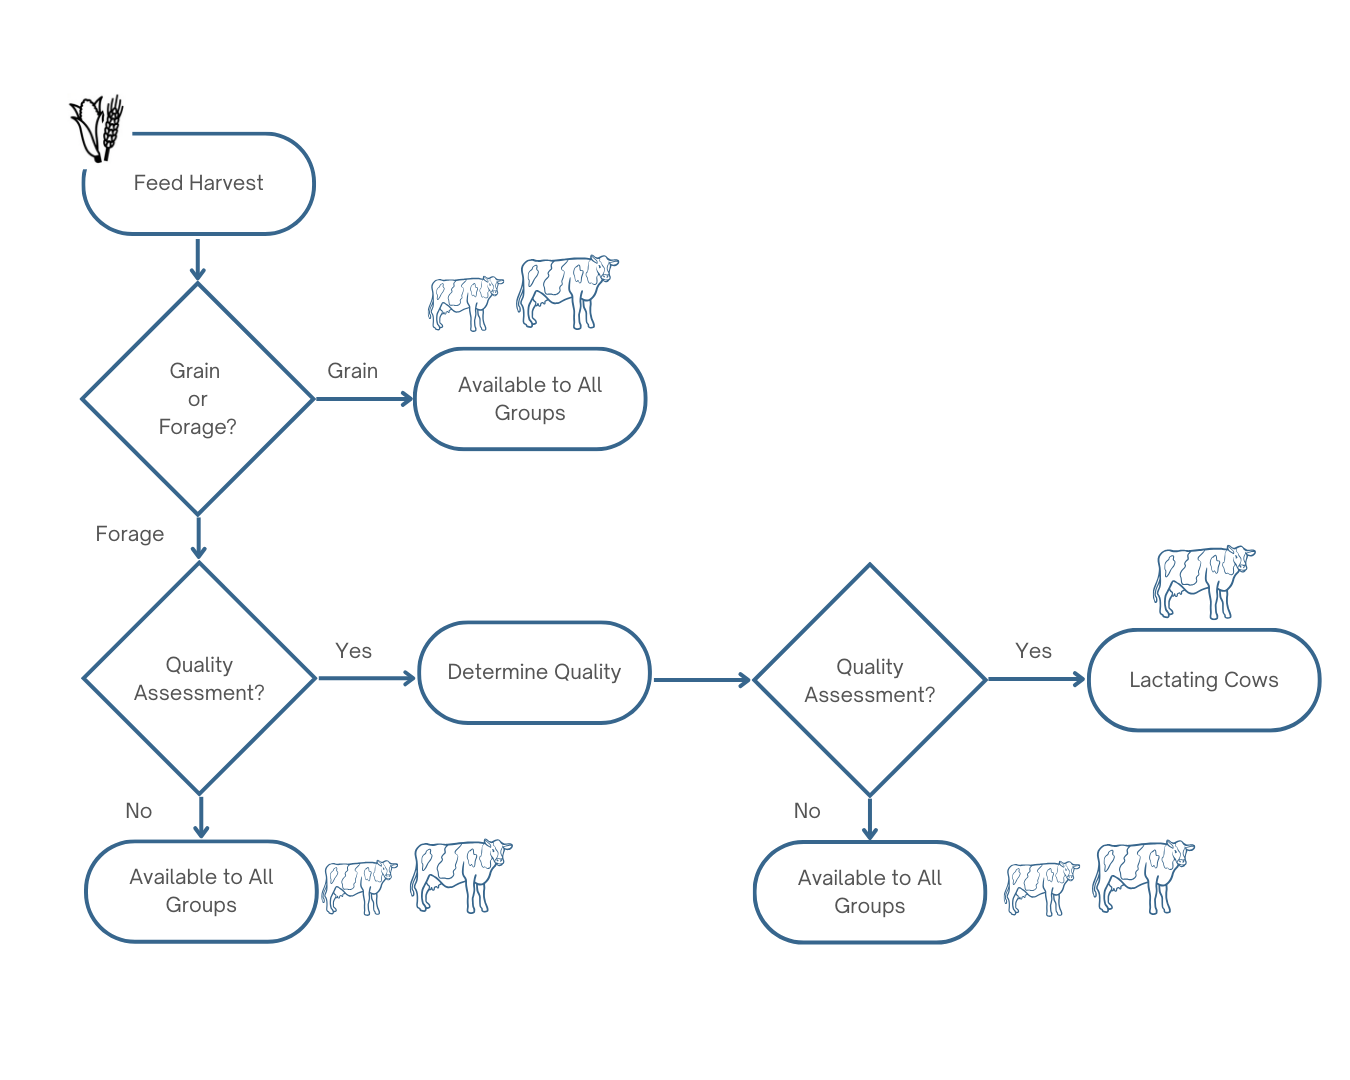
\includegraphics[width=0.9\textwidth]{resources/feedallocation.png} % Replace with your image file
    \caption{Farm grown feed allocation to cattle groups }
    \end{figure}


We currently represent the quality assessment for the feeds based on a single differentiating nutrient composition value. The differentiating nutrient and levels of the nutrient are given in the feed library.

The feed library that includes both NRC and NASEM feeds does not have feed quality embedded in the feed IDs. Instead, a quality assessment should be made independent of the feed ID number and added as an additional attribute of the stored feed. 

\section{Feed Storage Inputs}
Farmgrown feeds have storage inputs that are described in depth below and consist of the following:
\begin{itemize}
    \item storage classification The class of storage: Grain, Hay, Silage, Baleage.
    \item name  Each storage has a unique name. Ex. "alfalfa\_silage\_storage\_1"
    \item crop\_name The name of the crop being stored.
    \item field\_name    The name of the field the crop was grown in.
    \item storage\_type  The sub-type of the storage class. Ex. "Dry" for grain storage
    \item dm\_loss\_coefficient An input used for grain storages that specifies a loss of DM. Ex. "0.01",
    \item initial\_storage\_dry\_matter The dry matter content upon receipt by the feed storage module.
    \item post\_wilting\_moisture\_percentage The DM content of silage or baleage after wilting.
    \item target\_dry\_matter The final DM content of hay.
    \item additional\_dry\_matter\_loss\_coefficient An optional input to represent DM loss in excess of normal processes.
    \item bale\_size An input used for baleage to specify the diameter of the bale in meters.
    \item rufas\_id The RuFaS feed ID of the stored crop.
    \item capacity 1e10 The maximum mass capacity of the storage.
\end{itemize}

\section{Storage Classifications}
The agricultural production of harvested animal feed is dependent on season, climate, and farm management. In most cases, this means that feed is produced in large quantities when growing conditions are suitable and must be preserved to meet daily animal feed requirements. Microbial spoilage of wet feed products rapidly degrades their nutritional quality and can harm livestock that consume spoiled feed. Viable, cost-effective methods of preservation depend on the crop type and climate, but practically are limited to drying feed beyond the ability to support microbial growth and fermenting feed in the absence of oxygen to produce acid and reduce pH to inhibit spoilage. Feed Storage functions are primarily based on those in the \href{https://www.ars.usda.gov/northeast-area/up-pa/pswmru/docs/integrated-farm-system-model/}{Integrated Farm Systems Model} but modified to accommodate a daily time-step and remove explicit spatial components.



\subsection{Grain} Grains (e.g., corn, rice, soybeans, and wheat) under 15\% moisture are considered dry grain. Higher moisture grains are considered high-moisture. Field harvested grains are not always sufficiently dry for safe storage (\(<\) 15\% moisture) and supplemental drying is often used to achieve target moisture content. Air-drying is a lower-energy drying method for drying grain to ambient levels that consists of passing ambient air through wet grains via fan. Heated-air drying is higher-energy and faster than air-drying, but can reduce moisture below ambient levels. In practice, DM loss from grains are small and are modeled as a fixed percentage loss of dry matter; 1\% for dry grain, 5\% for high-moisture grain.


    \begin{center}
        \(L\_\{gaseous\}  = M\_i\ cdot 0.01\ tag\)
    \end{center}
        \vspace{0.5cm}
    
            {\raggedleft \textbf{[FS.GRN.1]}\par}
            \vspace{0.5cm}

    \begin{center}
        \(L\_\{gaseous\}  = M\_i\ cdot 0.05\ tag\)
    \end{center}
        \vspace{0.5cm}
    
            {\raggedleft \textbf{[FS.GRN.2]}\par}
            \vspace{0.5cm}
            
High-moisture grain as a feed must be managed (fed, fermented, or dried) quickly for this to be accurate, but that is a well-understood requirement and is not explicitly modeled. Nutritional quality changes are variable, but proportional to DM loss. Nutrient values of finished grain not currently tracked are referenced from the most recent edition of NASEM for use in the Animal Module.

\subsection{Hay} Hay is forage that has been dried with a safe preservation moisture content of 12-15\%. Bale storage conditions are separated into protected and unprotected storage with a total of four storage categories in order of decreasing protection from the elements: protected-indoor, protected-wrapped, protected-tarped, and unprotected-outdoor. Less protected hay storages experience additional losses as compared to the most protected storage (indoor) due to exposure to increased airflow and weather according to the following equation. Baled hay loses DM and quality as a function of storage conditions and its moisture content. Bale density plays a role, but is too complex to model directly and is instead estimated as a function of moisture content.

    \begin{center}
        \(L\_\{gaseous\}  = L\_\{base\} + L\_\{additional\}\ tag\)
    \end{center}
        \vspace{0.5cm}
    
            {\raggedleft \textbf{[FS.HAY.1]}\par}
            \vspace{0.5cm}


\textbf{Where we know that}: \\ L\_\{base\} (kg) is the minimum loss expected from protected-indoor as the sum of DM lost in the first 30 days of storage (L\_\{first 30 days\}, kg) and that lost after 30 days (L\_\{post 30 days\}, kg) in order to capture the differing rates of DM loss before and after the forage has reached its target DM content.

    \begin{center}
        \(L\_\{base\}  =  L\_\{first\ 30\ days\} + L\_\{post\ 30\ days\}\ tag\)
    \end{center}
        \vspace{0.5cm}
    
            {\raggedleft \textbf{[FS.HAY.2]}\par}
            \vspace{0.5cm}

\textbf{Where we know that}: \\ 
    \begin{center}
        \(L\_\{first\ 30\ days\} =  \frac{Q + 2433 \cdot [moisture - \frac{MF(1 - moisture)}{1 - MF}]}{(1 - moisture)(14206 - \frac{2433 \cdot MF}{1 - MF})} \cdot \frac{min(30, d)}{30} \ tag\)
    \end{center}
        \vspace{0.5cm}
    
            {\raggedleft \textbf{[FS.HAY.3]}\par}
            \vspace{0.5cm}

    \begin{center}
        \(Q =  104 \cdot moisture^{2.18} \cdot {b_{density}}^{0.5} + 5.72(moisture^{1.23} \cdot {b_{density}}^{0.94})\ tag\)
    \end{center}
        \vspace{0.25cm}
        \textit{Q is the sensible heat generated in the hay (kJ/kg) based on bale density}
        \vspace{0.5cm}
    
            {\raggedleft \textbf{[FS.HAY.4]}\par}
            \vspace{0.5cm}

    \begin{center}
        \(b\_\{density\} =  100 + 440 \cdot moisture\ tag\)
    \end{center}
        \vspace{0.5cm}
    
            {\raggedleft \textbf{[FS.HAY.5]}\par}
            \vspace{0.5cm}

moisture is the fraction of water mass at time of storage (unitless), MF is the target final moisture percent of hay (percent) as defined by the user (default: 12), and d is the number of days the hay has been stored for. 
\vspace{0.2cm}

And
\vspace{0.5cm}

    \begin{center}
        \(L\_\{post\ 30\ days\} =  0.0001 \cdot max(0, d - 30)\ tag\)
    \end{center}
        \vspace{0.5cm}
    
            {\raggedleft \textbf{[FS.HAY.6]}\par}
            \vspace{0.5cm}

        \begin{center}
        \(L\_\{additional\} =  \sum_{i=1}^{d} l \cdot rain_i \cdot max(0.0, \frac{high_i + low_i}{2}) \cdot \frac{1}{b_{density}} \cdot {b_{size}}^3\ tag\)
    \end{center}
        \vspace{0.5cm}
    
            {\raggedleft \textbf{[FS.HAY.7]}\par}
            \vspace{0.5cm}

        \begin{itemize}
            \item d is the number of days the hay has been stored for, 
            \item i is the day of storage that dry matter loss is being calculated for, 
            \item l is the loss coefficient (unitless) from Table 1; \textbf{[FS.HAY.7]}, 
            \item{rain\_i} is the amount of rain on day i (cm), 
            \item{high\_i} is the high temperature on day i (\(\circ C\)), 
            \item{low\_i} is the low temperature on day (\(\circ C\)), 
            \item{b\_density} is the bale density (kg/\(m^2\)) \textbf{[FS.HAY.5]}, and 
            \item{b\_size} is the diameter of the hay bale (m)

        \end{itemize}
\vspace{0.5cm}

\begin{table}[h!]
\centering
\renewcommand{\arraystretch}{1.3}
\caption{Hay storage types and associated fractional loss coefficients}

\begin{tabular}{@{} C{5cm} C{4cm}  @{}}
\toprule
\textbf{Hay Storage Type} & \textbf{Fractional Loss Coefficient (i)}  \\
\midrule
Protected Wrapped & 0.0000216 \\ 
Protected Tarped & 0.0000108 \\
Unprotected Outdoor  & 0.00006 \\
Protected Indoor  & 0 \\
\bottomrule
\end{tabular}
\end{table}

\vspace{1cm}

        \textit{Cumulative water lost from forages stored as hay is determined by:}
        \vspace{0.2cm}

        \begin{center}
        \(M =  F_i \cdot \frac{max(0.0, moisture - MF)}{100} \cdot \frac{min(30, d)}{30}\ tag\)
    \end{center}
        \vspace{0.5cm}
    
            {\raggedleft \textbf{[FS.HAY.8]}\par}
            \vspace{0.5cm}

The lowest energy method for hay drying is passive drying in the field when conditions are suitable, but, similarly to grains, hay can receive supplemental drying via ambient or heated air.  DM loss from protected, baled hay is preferentially from starch and water soluble carbohydrates (60\%), and CP (40\%) which, over time, leads to a proportional increase in NDF and a minor increase in CP over time. Unprotected bales experience increased proportional CP loss (50\% of protected bale DM loss) due to leaching and an additional 17\% loss of NDF dry matter compared to protected bales. Fractional loss coefficients for hay are defined by Table 2:
\vspace{0.5cm}

\begin{table}[h!]
\centering
\renewcommand{\arraystretch}{1.3}
\caption{Protected and unprotected storage, nutrients, and associated fractional loss coefficients}

\begin{tabular}{@{} L{5cm} L{4cm} L{3cm} @{}}
\toprule
\textbf{Hay Storage Type} & \textbf{Nutrient} & \textbf{Fractional Loss Coefficient}  \\
\midrule

\multirow{3}{*}{Unprotected Hay} & Acid Detergent Fiber & 0.0 \\
                           & Neutral Detergent Fiber & 0.17 \\
                           & Crude Protein & 0.4 \\
\multirow{3}{*}{Protected or Indoor Hay} & Acid Detergent Fiber & 0.0 \\
                           & Neutral Detergent Fiber & 0.0 \\
                           & Crude Protein & 0.0 \\
                           
                           
\bottomrule
\end{tabular}
\end{table}
\vspace{1cm}


\subsection{Silage} Silage is the product of anaerobic acidification of non-dry forage, a process called ensiling, and has traditionally been produced as a method of animal feed preservation viable in wet, cool climates where forage production cannot sustain livestock year-round and drying hay at the required scale is challenging \parencite{pahlow2003microbiology}. Typically, forage fermentation is the product of lactic acid bacteria (LAB) consuming WSC present in harvested forage and metabolizing it to a mix of organic products, including the desirable lactic and acetic acids, as well as \(CO_2\) and ethanol. A well-preserved silage relies on a rapid fermentation for retention of optimal feed quality because insufficient or slow acidification is associated with prolonged proteolytic activity, additional dry matter loss, and increased risk of spoilage. \parencite{pahlow2003microbiology, muck2013recent}.

Fermented forages experience DM loss and nutrient changes post-harvest, during fermentation, and during storage. Wilting losses are not currently modeled.


Alfalfa fermentation daily dry matter loss (fraction) is calculated with the equation:


        \begin{center}
        \(L\_{fermentation} = \sum_{i=1}^{d} drymass_{i-1} \cdot (0.00052 - 0.001213(dryfrac_{i-1} - 0.2))\ tag\)
    \end{center}
        \vspace{0.5cm}
    
            {\raggedleft \textbf{[FS.SIL.1]}\par}
        \vspace{0.5cm}

        \begin{itemize}
            \item d is the number of days the alfalfa has been ensiled for, 
            \item i is the day since ensiling that dry matter loss is being calculated for, 
            \item drymass\_{i-1} is the dry matter mass of ensiled alfalfa on day i-1,
            \item dryfrac\_{i-1} is the fraction of ensiled alfalfa fresh mass that is dry matter on day i-1. 
            \item When i is 1, drymass\_{i-1} is the initial amount of ensiled alfalfa dry mass and 
            \item dryfrac\_{i-1} is the initial dry matter fraction of the ensiled alfalfa. This equation is only appropriate for use if dryfrac\_{i-1} is in the range [0.2, 0.6] and the average temperature on day 
            \item i is in the range [5, 45] (\(\circ C\)).
        \end{itemize}
        \vspace{0.5cm}
        
Corn, grass, and small grain daily dry matter loss (fraction) is calculated with the equation:
\vspace{0.2cm}

        \begin{center}
        \(L_{fermentation} = \sum_{i=1}^{d} drymass_{i-1} \cdot (0.000288 - 0.000643(dryfrac_{i-1} - 0.15))\ tag\)
    \end{center}
        \vspace{0.5cm}
    
            {\raggedleft \textbf{[FS.SIL.2]}\par}
        \vspace{0.5cm}

        \begin{itemize}
            \item d is the number of days the forage has been ensiled for, 
            \item i is the day since ensiling that dry matter loss is being calculated for, 
            \item drymass\_{i-1} is the dry matter mass of ensiled forage on day i-1,
            \item dryfrac\_{i-1} is the fraction of ensiled forage fresh mass that is dry matter on day i-1. 
            \item When i is 1, drymass\_{i-1} is the initial amount of ensiled forage dry mass and 
            \item dryfrac\_{i-1} is the initial dry matter fraction of the ensiled forage. This equation is only appropriate for use if dryfrac\_{i-1} is in the range [0.15, 0.6] and the average temperature on day i is in the range [0, 40] (\(\circ C\)).
        \end{itemize}

\begin{table}[h!]
\centering
\renewcommand{\arraystretch}{1.3}
\caption{Silage and the fractional loss coefficients}

\begin{tabular}{@{} L{5cm} L{4cm} L{3cm} @{}}
\toprule
\textbf{Nutrient} & \textbf{Fractional Loss Coefficient}  \\
\midrule

Acid Detergent Fiber & 0.0 \\
Neutral Detergent Fiber & 0.0 \\
Crude Protein & 0.0 \\
                           
                         
\bottomrule
\end{tabular}
\end{table}
\vspace{1CM}

Ensiled crops may also lose dry matter through effluent efflux. Crops that are ensiled with a dry matter content less than 30\% lose both water and dry matter according to the following equations:
\vspace{0.25CM}

        \begin{center}
        \(L_{effluent} = dryfrac\_\{effluent\} \cdot M\_\{effluent\} \cdot 0.1 \cdot max(10, d)\ tag\)
    \end{center}
        \vspace{0.5cm}
    
            {\raggedleft \textbf{[FS.SIL.4]}\par}
        \vspace{0.5cm}
        
\textbf{Where we know that}: \\ 
\vspace{0.2cm}

\(dryfrac_{effluent}\) is the fraction of dry matter in the effluent that is lost, \(M_{effluent}\) is the estimated maximum effluent (kg), and d is the number of days the crop has been ensiled for.
\vspace{0.5cm}

        \begin{center}
        \(ML\_\{effluent\} = (1 - dryfrac_{effluent}) \cdot M_{effluent} \cdot 0.1 \cdot max(10, d) \ tag\)
        \end{center}
        \vspace{0.5cm}
    
            {\raggedleft \textbf{[FS.SIL.5]}\par}
        \vspace{0.5cm}

\textbf{Where we know that:} dryfrac\_{effluent} is the fraction of dry matter in the effluent that is lost,
        \vspace{0.2cm}

M\_{effluent} is the estimated maximum effluent (kg), and d is the number of days the crop has been ensiled for. The fraction of dry matter in effluent is a constant defined as: 
\vspace{0.2cm}

        \begin{center}
        \(dryfrac_{effluent} = 0.1035\ tag\)
    \end{center}
        \vspace{0.5cm}
    
            {\raggedleft \textbf{[FS.SIL.6]}\par}
        \vspace{0.5cm}
        
        \begin{center}
        \(M_{effluent} = mass_{fresh} \cdot ((1 - dryfrac) - 0.7) \ tag\)
    \end{center}
        \vspace{0.5cm}
    
            {\raggedleft \textbf{[FS.SIL.7]}\par}
        \vspace{0.5cm}


\textbf{Where we know that}: \\ \(mass_{fresh}\) is the fresh mass of the crop when it is ensiled (kg) and 
\(dryfrac\) is the fraction of the crop’s fresh mass which is dry matter when it is ensiled.
\vspace{0.2cm}

Dry matter lost in effluent is preferentially from CP, water soluble carbohydrates, and non-protein nitrogen each of which is recalculated by the following equations:
\vspace{0.2cm}

Percent crude protein is calculated as:
\vspace{0.2cm}
        
        \begin{center}
        \(CP_{updated} = \frac{CP_{initial} \cdot 0.01 - 0.3 \cdot DL_{fraction}}{1 - DL_{fraction}} \cdot 100 \ tag\)
    \end{center}
        \vspace{0.5cm}
    
            {\raggedleft \textbf{[FS.SIL.8]}\par}
        \vspace{0.5cm}

\textbf{Where we know that}: \\ \(CP_{initial}\) is the percentage of dry matter mass that is crude protein in the ensiled crop before accounting for dry matter loss to effluent and \(DL_{fraction}\) is the fraction of dry matter mass lost to effluent. The percentage of crude protein is lower-bounded at 0.
\vspace{0.2cm}

The percentage of NPN is calculated with the equation:
\vspace{0.2cm}

        \begin{center}
        \(NPN_{updated} = \frac{(NPN_{initial} \cdot 0.01) \cdot (CP_{initial} \cdot 0.01) - 0.3 \cdot DL_{fraction}}{(CP_{initial} \cdot 0.01) - DL_{fraction}} \cdot 100 \ tag\)
    \end{center}
        \vspace{0.5cm}
    
            {\raggedleft \textbf{[FS.SIL.9]}\par}
        \vspace{0.5cm}


\textbf{Where we know that}: \\ \(NPN_{initial}\) is percentage of dry matter mass that is non-protein nitrogen in the ensiled crop before accounting for dry matter loss to effluent, \(CP_{initial}\) is the percentage of dry matter mass that is crude protein before accounting for dry matter loss to effluent, and \(DL_{fraction}\) is the fraction of dry matter mass lost to effluent. The percentage of non-protein nitrogen is lower-bounded at 0. 
\vspace{0.2cm}

\(DL_{fraction}\) is calculated with the equation:
        \begin{center}
        \(DL_{fraction} = \frac{DM_{lost}}{DM_{initial}}\ tag\)
    \end{center}
        \vspace{0.5cm}
    
            {\raggedleft \textbf{[FS.SIL.10]}\par}
        \vspace{0.5cm}

\textbf{Where we know that}: \\ DM\_lost is the amount of dry matter mass in the ensiled crop after accounting for dry matter lost to effluent, and DM\_initial is the amount of dry matter mass in the ensiled crop before accounting for dry matter lost to effluent.

\subsection{Baleage}
Baleage is an ensiled forage with a DM content between 50-65\% that is baled and wrapped to allow ensiling. The higher DM content of baleage lowers the amount of acid needed to achieve effective preservation and allows it to be consolidated into a bale. Fermentation DM losses for baleage are calculated by \textbf{[FS.SIL.1]} and \textbf{[FS.SIL.2]} with fractional nutrient loss coefficients from Table 3. Baleage does not experience effluent losses.

\subsection{Nutrient Composition}
Changes in dry matter and moisture of stored feed often alter their total and fractional nutrient composition. Recalculating nutrient fractions of stored feeds uses the following equation:
\vspace{0.2cm}

        \begin{center}
        \(n_{updated} = \frac{max(0, \frac{n_{initial}}{100} - C) \cdot DL_{fraction}}{1 - DL_{fraction}} \cdot 100 \ tag\)
    \end{center}
        \vspace{0.5cm}
    
            {\raggedleft \textbf{[FS.NUT.1]}\par}
        \vspace{0.5cm}

\textbf{Where we know that}: \\ n\_updated is the percentage of the target nutrient in the stored crop’s dry matter mass after accounting for dry matter loss, n\_initial is the percentage of the target nutrient in the stored crop’s dry matter mass before accounting for dry matter loss, C is the fractional loss coefficient specific to the nutrient and storage type, and DL\_fraction is the fraction of dry matter lost.
\vspace{0.2cm}

        \begin{center}
        \(DL_{fraction} = \frac{DM_{updated}}{DM_{initial}} \ tag\)
    \end{center}
        \vspace{0.5cm}
    
            {\raggedleft \textbf{[FS.NUT.2]}\par}
        \vspace{0.5cm}







\newpage
\section{References}
\printbibliography[heading=subbibliography,title={Feed Storage Module}]
\end{refsection}


\newpage
\part{Abbreviations}

\renewcommand{\arraystretch}{1.3}
\newcolumntype{L}[1]{>{\RaggedRight\arraybackslash}p{#1}}

% optionally tighten column padding just for this table
\setlength{\tabcolsep}{4pt}

\begin{longtable}{@{} L{0.23\textwidth} L{0.70\textwidth} @{}} % 0.93*textwidth + padding < textwidth
\caption{Common abbreviations used throughout this document} \\

\toprule
\textbf{Abbreviation} & \textbf{Full Term or Phrase} \\
\midrule
\endfirsthead

\multicolumn{2}{@{}l}{\textit{Table continued from previous page}} \\
\toprule
\textbf{Abbreviation} & \textbf{Full Term or Phrase} \\
\midrule
\endhead

\midrule
\multicolumn{2}{@{}r@{}}{\textit{Continued on next page}} \\
\endfoot

\bottomrule
\endlastfoot

ADF & Acid detergent fiber (\% of DM) \\
ADG & Average daily weight gain (g/d) \\
Age1stBred & First breeding age (month) \\
BCS5 & Body condition score (1–5 basis) \\
BW & Body weight (kg) \\
Ca & Calcium content (\% of DM) \\
CBW & Calf birth weight (kg) \\
CI & Calving interval (d) \\
cm & centimeter \\
Cost & Feed cost (\$/kg of DM) \\
CP & Crude protein (\% of DM) \\
d & days \\
DE & Digestible energy (standard value, Mcal/kg) \\
DIM & Days in milk \\
DM & Dry matter (\% of as-fed basis) \\
DMI & Dry matter intake \\
DOP & Days of pregnancy (d) \\
dRUP & RUP degradability (\% of RUP) \\
EE & Ether extract, in crude fat (\% DM) \\
EndCP & Endogenous CP \\
EndN & Endogenous N \\
EQSBW & Equivalent shrunk body weight (kg) \\
FA & Fatty acids \\
FIPS & Federal Information Processing Standards \\
g & grams \\
GE & Gross energy (standard value, Mcal/kg) \\
GrUterW & Gravid uterine weight (kg) \\
Kd & Rumen protein degradation rate (\%/h) \\
kg & kilograms \\
kJ & kilojoule \\
L & liters \\
m & meter \\
max & maximum \\
Mcal & Megacalorie \\
MCP & Microbial Crude Protein \\
ME & Metabolizable energy (standard value, Mcal/kg) \\
MICP & Microbial CP \\
min & minimum \\
mL & milliliters \\
MN & Microbial N \\
MP & Metabolizable protein \\
MTP & Microbial TP \\
MW & Mature body weight (kg) \\
MY & Milk yield \\
N & Nitrogen (\% of DM) \\
NASEM & National Academies of Sciences, Engineering, and Medicine \\
NDF & Neutral detergent fiber (\% of DM) \\
NEG & Net energy for growth (standard value, Mcal/kg) \\
NEL & Net energy for lactation (standard value, Mcal/kg) \\
NEM & Net energy for maintenance (standard value, Mcal/kg) \\
nNDF & Nondigestible Neutral Detergent Fiber \\
NPN & Non-protein Nitrogen \\
NRC & National Research Council (updated in 2021 to NASEM) \\
OM & Organic matter (\% of DM) \\
P & Phosphorus content (\% of DM) \\
PAF & Processing adjustment factor (not used) \\
Parity & Number of lactations \\
PrevTemp & Average daily temperature of last month (°C) \\
RDP & Ruminally degraded CP \\
ROM & Residual OM (\% of DM) \\
RUP & Ruminally undegraded CP \\
s & seconds \\
TAN & Total ammoniacal N \\
TDN & Total digestible nutrient (\% of DM) \\
TP & True protein (\% of DM) \\
USDA & United States Department of Agriculture \\
UterW & Uterine weight (kg) \\
WSC & Water Soluble Carbohydrates \\
\end{longtable}

\end{document}
